% Options for packages loaded elsewhere
% Options for packages loaded elsewhere
\PassOptionsToPackage{unicode}{hyperref}
\PassOptionsToPackage{hyphens}{url}
\PassOptionsToPackage{dvipsnames,svgnames,x11names}{xcolor}
%
\documentclass[
  english,
]{article}
\usepackage{xcolor}
\usepackage{amsmath,amssymb}
\setcounter{secnumdepth}{5}
\usepackage{iftex}
\ifPDFTeX
  \usepackage[T1]{fontenc}
  \usepackage[utf8]{inputenc}
  \usepackage{textcomp} % provide euro and other symbols
\else % if luatex or xetex
  \usepackage{unicode-math} % this also loads fontspec
  \defaultfontfeatures{Scale=MatchLowercase}
  \defaultfontfeatures[\rmfamily]{Ligatures=TeX,Scale=1}
\fi
\usepackage{lmodern}
\ifPDFTeX\else
  % xetex/luatex font selection
\fi
% Use upquote if available, for straight quotes in verbatim environments
\IfFileExists{upquote.sty}{\usepackage{upquote}}{}
\IfFileExists{microtype.sty}{% use microtype if available
  \usepackage[]{microtype}
  \UseMicrotypeSet[protrusion]{basicmath} % disable protrusion for tt fonts
}{}
\makeatletter
\@ifundefined{KOMAClassName}{% if non-KOMA class
  \IfFileExists{parskip.sty}{%
    \usepackage{parskip}
  }{% else
    \setlength{\parindent}{0pt}
    \setlength{\parskip}{6pt plus 2pt minus 1pt}}
}{% if KOMA class
  \KOMAoptions{parskip=half}}
\makeatother
% Make \paragraph and \subparagraph free-standing
\makeatletter
\ifx\paragraph\undefined\else
  \let\oldparagraph\paragraph
  \renewcommand{\paragraph}{
    \@ifstar
      \xxxParagraphStar
      \xxxParagraphNoStar
  }
  \newcommand{\xxxParagraphStar}[1]{\oldparagraph*{#1}\mbox{}}
  \newcommand{\xxxParagraphNoStar}[1]{\oldparagraph{#1}\mbox{}}
\fi
\ifx\subparagraph\undefined\else
  \let\oldsubparagraph\subparagraph
  \renewcommand{\subparagraph}{
    \@ifstar
      \xxxSubParagraphStar
      \xxxSubParagraphNoStar
  }
  \newcommand{\xxxSubParagraphStar}[1]{\oldsubparagraph*{#1}\mbox{}}
  \newcommand{\xxxSubParagraphNoStar}[1]{\oldsubparagraph{#1}\mbox{}}
\fi
\makeatother


\usepackage{longtable,booktabs,array}
\usepackage{calc} % for calculating minipage widths
% Correct order of tables after \paragraph or \subparagraph
\usepackage{etoolbox}
\makeatletter
\patchcmd\longtable{\par}{\if@noskipsec\mbox{}\fi\par}{}{}
\makeatother
% Allow footnotes in longtable head/foot
\IfFileExists{footnotehyper.sty}{\usepackage{footnotehyper}}{\usepackage{footnote}}
\makesavenoteenv{longtable}
\usepackage{graphicx}
\makeatletter
\newsavebox\pandoc@box
\newcommand*\pandocbounded[1]{% scales image to fit in text height/width
  \sbox\pandoc@box{#1}%
  \Gscale@div\@tempa{\textheight}{\dimexpr\ht\pandoc@box+\dp\pandoc@box\relax}%
  \Gscale@div\@tempb{\linewidth}{\wd\pandoc@box}%
  \ifdim\@tempb\p@<\@tempa\p@\let\@tempa\@tempb\fi% select the smaller of both
  \ifdim\@tempa\p@<\p@\scalebox{\@tempa}{\usebox\pandoc@box}%
  \else\usebox{\pandoc@box}%
  \fi%
}
% Set default figure placement to htbp
\def\fps@figure{htbp}
\makeatother



\ifLuaTeX
\usepackage[bidi=basic]{babel}
\else
\usepackage[bidi=default]{babel}
\fi
% get rid of language-specific shorthands (see #6817):
\let\LanguageShortHands\languageshorthands
\def\languageshorthands#1{}
\ifLuaTeX
  \usepackage[english]{selnolig} % disable illegal ligatures
\fi


\setlength{\emergencystretch}{3em} % prevent overfull lines

\providecommand{\tightlist}{%
  \setlength{\itemsep}{0pt}\setlength{\parskip}{0pt}}



 


\usepackage{hyphenat}
\usepackage{graphicx}
% and their extensions so you won't have to specify these with
 % every instance of \includegraphics
 \usepackage{pdfcomment}
\DeclareGraphicsExtensions{.pdf,.jpeg,.png}
\usepackage{wallpaper} % for the background image on title page
\usepackage{geometry}
% set font

%\usepackage{lmodern}
%\usepackage[T1]{fontenc}

\usepackage{fontspec}
%\setsansfont[Ligatures=TeX]{Arial Narrow}
\setsansfont[Ligatures=TeX]{Times New Roman}

%\newfontfamily\sectionfont[Color=Black]{Latin Modern Sans}
%\newfontfamily\subsectionfont[Color=Black]{Latin Modern Sans}
%\newfontfamily\subsubsectionfont[Color=Black]{Latin Modern Sans}

%\usepackage[headsepline=0.005pt:,footsepline=0.005pt:,plainfootsepline,automark]{scrlayer-scrpage}
%\clearpairofpagestyles
%\ohead[]{\headmark} \cofoot[\pagemark]{\pagemark}
%\lohead{Assessment of U.S. West Coast Sablefish in 2025}
%\ModifyLayer[addvoffset=-.6ex]{scrheadings.foot.above.line}
%\ModifyLayer[addvoffset=-.6ex]{plain.scrheadings.foot.above.line}
%\setkomafont{pageheadfoot}{\small}

\usepackage{pdfpages}
\usepackage{float}
\let\origfigure\figure
\let\endorigfigure\endfigure
\renewenvironment{figure}[1][2] {
    \expandafter\origfigure\expandafter[H]
} {
    \endorigfigure
}
% Landscape tables and figures
\usepackage{pdflscape}
\newcommand{\blandscape}{\begin{landscape}}
\newcommand{\elandscape}{\end{landscape}}

% Acronyms
\usepackage[acronym]{glossaries}
\glsdisablehyper
\loadglsentries{sa4ss_glossaries.tex}

\usepackage{tikz}
\usepackage{booktabs}
\usepackage{longtable}
\usepackage{array}
\usepackage{multirow}
\usepackage{wrapfig}
\usepackage{float}
\usepackage{colortbl}
\usepackage{pdflscape}
\usepackage{tabu}
\usepackage{threeparttable}
\usepackage{threeparttablex}
\usepackage[normalem]{ulem}
\usepackage{makecell}
\usepackage{xcolor}
\makeatletter
\@ifpackageloaded{caption}{}{\usepackage{caption}}
\AtBeginDocument{%
\ifdefined\contentsname
  \renewcommand*\contentsname{Table of contents}
\else
  \newcommand\contentsname{Table of contents}
\fi
\ifdefined\listfigurename
  \renewcommand*\listfigurename{List of Figures}
\else
  \newcommand\listfigurename{List of Figures}
\fi
\ifdefined\listtablename
  \renewcommand*\listtablename{List of Tables}
\else
  \newcommand\listtablename{List of Tables}
\fi
\ifdefined\figurename
  \renewcommand*\figurename{Figure}
\else
  \newcommand\figurename{Figure}
\fi
\ifdefined\tablename
  \renewcommand*\tablename{Table}
\else
  \newcommand\tablename{Table}
\fi
}
\@ifpackageloaded{float}{}{\usepackage{float}}
\floatstyle{ruled}
\@ifundefined{c@chapter}{\newfloat{codelisting}{h}{lop}}{\newfloat{codelisting}{h}{lop}[chapter]}
\floatname{codelisting}{Listing}
\newcommand*\listoflistings{\listof{codelisting}{List of Listings}}
\makeatother
\makeatletter
\makeatother
\makeatletter
\@ifpackageloaded{caption}{}{\usepackage{caption}}
\@ifpackageloaded{subcaption}{}{\usepackage{subcaption}}
\makeatother
\usepackage{bookmark}
\IfFileExists{xurl.sty}{\usepackage{xurl}}{} % add URL line breaks if available
\urlstyle{same}
\hypersetup{
  pdftitle={Summary of available Northwest Fisheries Science Center survey data to support assessments of U.S. West Coast groundfish stocks},
  pdfauthor={Chantel R. Wetzel; R. Claire Rosemond},
  pdflang={en},
  colorlinks=true,
  linkcolor={blue},
  filecolor={Maroon},
  citecolor={Blue},
  urlcolor={Blue},
  pdfcreator={LaTeX via pandoc}}


\title{Summary of available Northwest Fisheries Science Center survey
data to support assessments of U.S. West Coast groundfish stocks}
\author{Chantel R. Wetzel \and R. Claire Rosemond}
\date{2026-02-12}
\begin{document}
  \begin{titlepage}
  % This is a combination of Pandoc templating and LaTeX
  % Pandoc templating https://pandoc.org/MANUAL.html#templates
  % See the README for help

  \newgeometry{top=2in,bottom=1in,right=1in,left=1in}
  \begin{minipage}[b][\textheight][s]{\textwidth}
  % Ross would've subbed lines 6, 8 with these lines:
  %\newgeometry{top=2in,bottom=1in,right=1in,left=1in}%
  %\noindent  %\tracingall
  %\begin{minipage}[b][\textheight][s]{.975\textwidth}%% RRM: avoid Overfull box


  \raggedright

  % \includegraphics[width=2cm]{NOAA_Transparent_Logo.png}

  % background image


  % Title and subtitle
  {\huge\bfseries\nohyphens{Summary of available Northwest Fisheries
  Science Center survey data to support assessments of U.S. West Coast
  groundfish stocks}}\\[1\baselineskip]
  % Ross would change the end of the above line to the following because \par must come before the group closes and line-depth reverts.
  % }\par}%\\[1\baselineskip]



  \vspace{1\baselineskip}
  % Ross would change this to 2\baselineskip

  %%%%%% Cover image

  \vspace{1\baselineskip}

  % Authors
  % This hairy bit of code is just to get "and" between the last 2
  % authors. See below if you don't need that
   {\large{Chantel R. Wetzel}}{\textsuperscript{1}}%
  %
  %
  { and \large{R. Claire Rosemond}}%
  {\textsuperscript{2}}%
  %


  % This is how to do it if you don't need the "and"

  %%%%%% Affiliations
  \vspace{2\baselineskip}

  \hangindent=1em
  \hangafter=1
  % Ross would change the above line to:
  % \hangafter=1\relax
  %
  {1}.~{NOAA Fisheries Northwest Fisheries Science Center}%
  %
  %
  % Ross recommends putting address on one line
  , %
  {2725 Montlake Boulevard East, Seattle, WA, 98112}%
  %
  \par\hangindent=1em\hangafter=1%
  %
  {2}.~{NOAA Fisheries Northwest Fisheries Science Center}%
  %
  %
  % Ross recommends putting address on one line
  , %
  {2032 SE OSU Drive Building 955, Newport, OR, 97365}%
  %


  %%%%%% Correspondence
  \vspace{1\baselineskip}


  %use \vfill instead to get the space to fill flexibly
  %\vspace{0.25\textheight} % Whitespace between the title block and the publisher

  \vfill


  % Whitespace between the title block and the tagline
  \vspace{1\baselineskip}

  %%%%%% Tagline at bottom
  % Ross says the tagline below could also be centered
  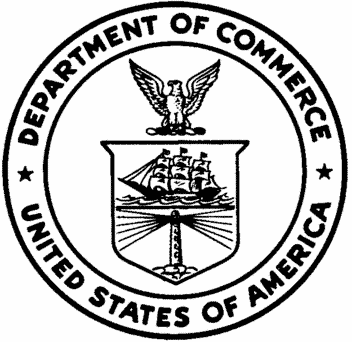
\includegraphics[alt={},width=2cm]{support_files/us_doc_logo.png}\newline % empty curly brackets without alt text is suitable for this logo because it's purely decorative/an "artifact"
  U.S. Department of Commerce\newline
  National Oceanic and Atmospheric Administration\newline
  National Marine Fisheries Service\newline
  Northwest Fisheries Science Center\newline

  \end{minipage}
  \restoregeometry
  \end{titlepage}


\newpage{}

Please cite this publication as:

Wetzel, C.R., and R.C. Rosemond. 2026. Summary of available Northwest
Fisheries Science Center survey data to support assessments of U.S. West
Coast groundfish stocks. Pacific Fisheries Management Council, Portland,
Oregon.

\newpage{}

\section*{Disclaimer}\label{disclaimer}

These materials do not constitute a formal publication and are for
information only. They are in a pre-review, pre-decisional state and
should not be formally cited or reproduced. They are to be considered
provisional and do not represent any determination or policy of NOAA or
the Department of Commerce.

\newpage{}

\hypersetup{linkcolor=.}
\setcounter{tocdepth}{3}
\tableofcontents

\newpage{}

\setlength{\parskip}{5mm plus1mm minus1mm}
\pagenumbering{arabic}
\setcounter{page}{1}
\setcounter{section}{0}
\renewcommand{\thefigure}{\arabic{figure}}
\renewcommand{\thetable}{\arabic{table}}
\setcounter{table}{0}
\setcounter{figure}{0}

\section{Introduction}\label{introduction}

This document provides a detailed summary of data sources that may be
used to support assessments in 2027. The data sources include the
Northwest Fisheries Science Center (NWFSC) West Coast Groundfish Bottom
Trawl Survey (WCGBTS) and NWFSC Hook-and-Line Survey (HKLS). A detailed
summary of data available by year for the species and associated stock
areas included in the Fishery Management Plan (FMP) can allow the
Pacific Fishery Management Council and advisory bodies to understand the
coverage of survey data across time and the potential viability of a new
assessment or assessment type.

This summary includes species-specific totals of available length and
age data for FMP species regularly sampled by federal surveys and only
in the associated stock areas listed in the FMP (or still under
consideration). For species with robust sampling, figures representing
relative indices of abundance and sampled length compositions by year
and source are also provided. A summary of the available maturity data
for each species is also listed.

This version of the data summary document does not include a summary of
commercial, recreational, or state-specific fishery-independent data.
Future versions may include information from these data sources, time
permitting.

\subsection{Biological Samples}\label{biological-samples}

Data collected by the WCGBTS between 2003-2025 and the HKLS from
2004-2025 are summarized by species. Summaries of the total lengths,
aged fish, and unread age structures collected by each survey and the
quantity available by year are provided. Additionally, the average
number of tows (WCGBTS) or set (HKLS) that observe each species by year
and survey is provided.

\subsection{Survey Length
Compositions}\label{survey-length-compositions}

The length data collected by the WCGBTS were expanded using a
generalized area-based stratification. The expanded length composition
data were summarized using either a 2 or 4 cm bin structure depending
upon the range between maximum and minimum lengths observed within the
survey data. All length observations were grouped as unsexed fish for
plotting to reveal potential trends in length compositions across time.

The length data collected by the HKLS were summarized to reflect the
proportion of observations by species, length bin, and year. The length
composition data were summarized using either a 2 or 4 cm bin structure
depending upon the range between maximum and minimum lengths observed
within the survey data, in the same manner as for the WCGBTS data.

The generalized approach for expanding the length composition data and
bin structure provides a simple summary of the data that can be useful
for decision making, but will likely differ from a species-specific
approach that would be applied in a future assessment. Additionally, it
is important to note that each survey's selectivity for each species
will impact the lengths observed and has not been explicitly accounted
for in this analysis.

\subsection{Survey Relative Indices of
Abundance}\label{survey-relative-indices-of-abundance}

Indices of abundance were estimated from the WCGBTS using a
spatiotemporal model (\texttt{sdmTMB}) for species well-observed by the
survey. The indices were estimated using a generalized configuration
across species using either a gamma, log-normal, or Tweedie
distribution, with the dispersion parameter held constant across years
with 200-500 knots used to create the mesh. The model structure for each
species is provided in Section \ref{wcgbt-index-settings}.
Species-specific indices of abundance produced for past assessments or
produced for future assessments may use a modified model structure
resulting in slight changes in year-by-year values for the indices of
abundance presented in this document.

Indices of abundance were estimated from the HKLS for well-observed
species using \texttt{sdmTMB} with a negative-binomial error structure
with covariates for year, site, and drop number. The model structure is
provided in Section \ref{hkl-index-settings}. Additional covariates or
error-structures to develop species-specific indices were not explored
in this analysis.

The indices of abundance presented here should only be considered
illustrative of potential trends in abundance across time.

\subsection{Maturity Data Collections}\label{maturity-data-collections}

Maturity samples for a wide range of West Coast groundfish species have
been collected across multiple sources: the WCGBTS, the HKLS, the
Pacific hake acoustic survey, at-sea sampling from the Pacific hake
fishery, and port sampling by state agencies. A summary of the number of
maturity samples collected and read between 2009 - 2024 is provided for
each species. These data summaries only include collections led by the
NWFSC but other collections could be available from other research
groups.

\newpage{}

\section{Groundfish species observed by surveys conducted by the
NWFSC}\label{groundfish-species-observed-by-surveys-conducted-by-the-nwfsc}

\subsection{Arrowtooth flounder}\label{arrowtooth-flounder}

The most recent assessment of arrowtooth flounder was an update
assessment conducted in 2017. Across available data, arrowtooth flounder
have been observed and sampled by the NWFSC WCGBTS. The NWFSC WCGBTS
observed arrowtooth flounder on an average of 226 tows per year. For
this species, a total of 254 maturity samples have been collected
coastwide (regardless of stock area), with 96 read maturities.

\begingroup\fontsize{10}{12}\selectfont
\begingroup\fontsize{10}{12}\selectfont

\begin{longtable}[t]{>{\raggedleft\arraybackslash}p{2cm}>{\raggedleft\arraybackslash}p{3.5cm}>{\raggedleft\arraybackslash}p{2cm}>{\raggedleft\arraybackslash}p{2cm}>{\raggedleft\arraybackslash}p{2cm}}
\caption{\label{tab:unnamed-chunk-3}Total number of available lengths, read ages, and unread age structures by data source and
state for arrowtooth flounder.}\\
\toprule
State & Source & Lengths & Ages & Age Structures\\
\midrule
\endfirsthead
\caption[]{Total number of available lengths, read ages, and unread age structures by data source and
state for arrowtooth flounder. (\textit{continued)}}\\
\toprule
State & Source & Lengths & Ages & Age Structures\\
\midrule
\endhead

\endfoot
\bottomrule
\endlastfoot
CA & NWFSC WCGBTS & 10,122 & 802 & 2,907\\
OR & NWFSC WCGBTS & 30,417 & 2,245 & 7,466\\
WA & NWFSC WCGBTS & 20,170 & 1,281 & 4,082\\*
\end{longtable}
\endgroup{}
\endgroup{}

\begin{figure}[H]

{\centering 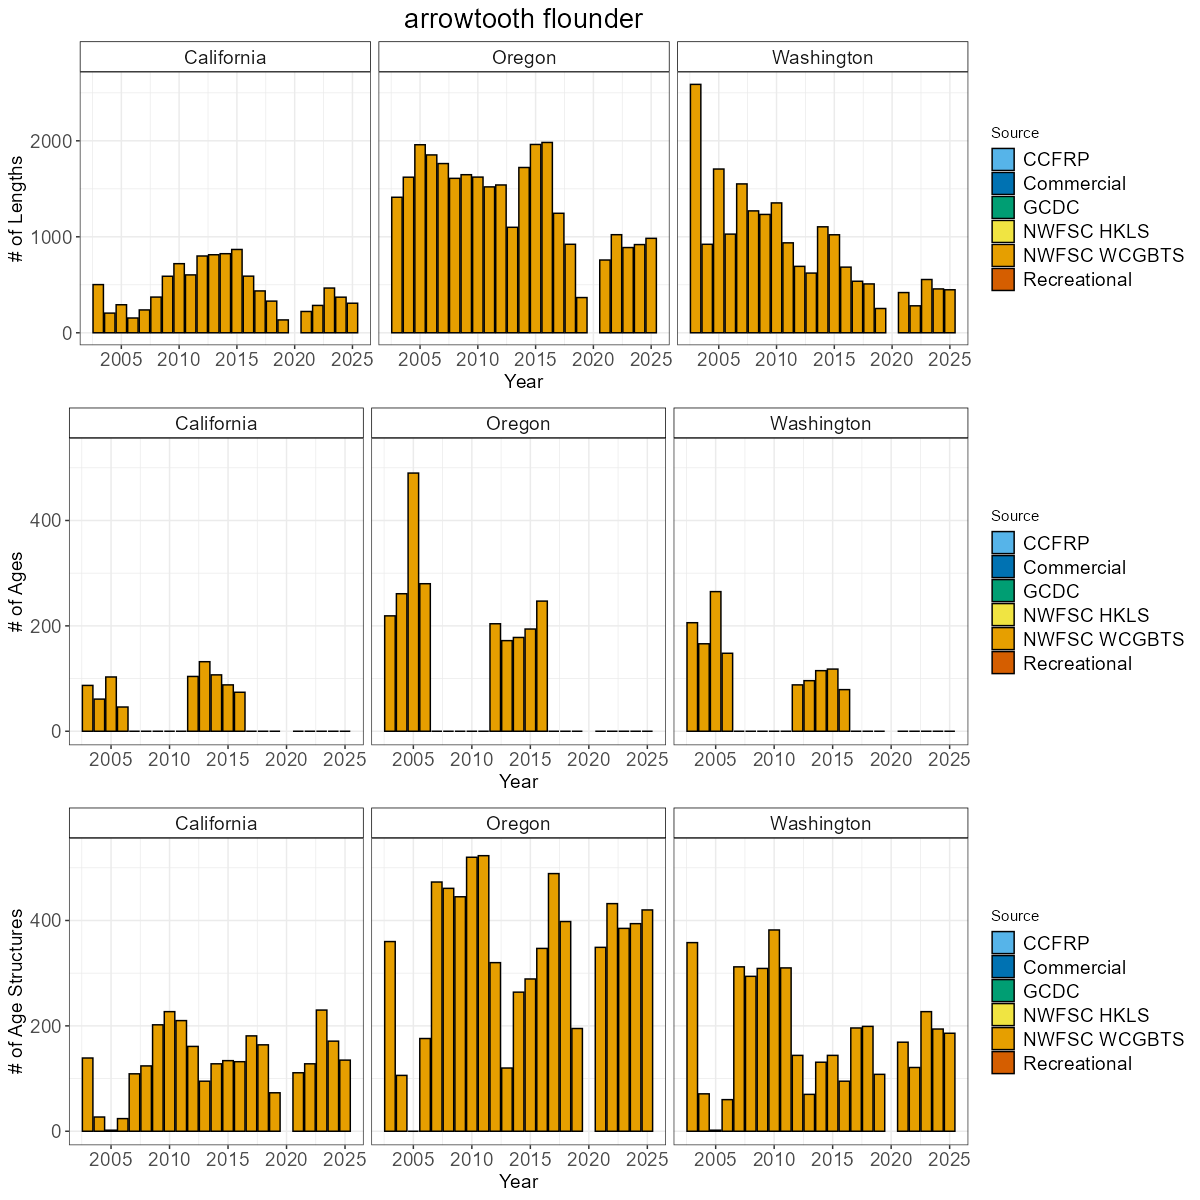
\includegraphics[width=0.95\linewidth,height=\textheight,keepaspectratio]{../plots/state_comparisons/arrowtooth_flounder_state_compositions.png}

}

\caption{Total number of available lengths, read ages, and unread age
structures by data source by year for arrowtooth flounder. Note the
y-axis maximum may differ by data type.}

\end{figure}%

\begin{figure}[H]

{\centering 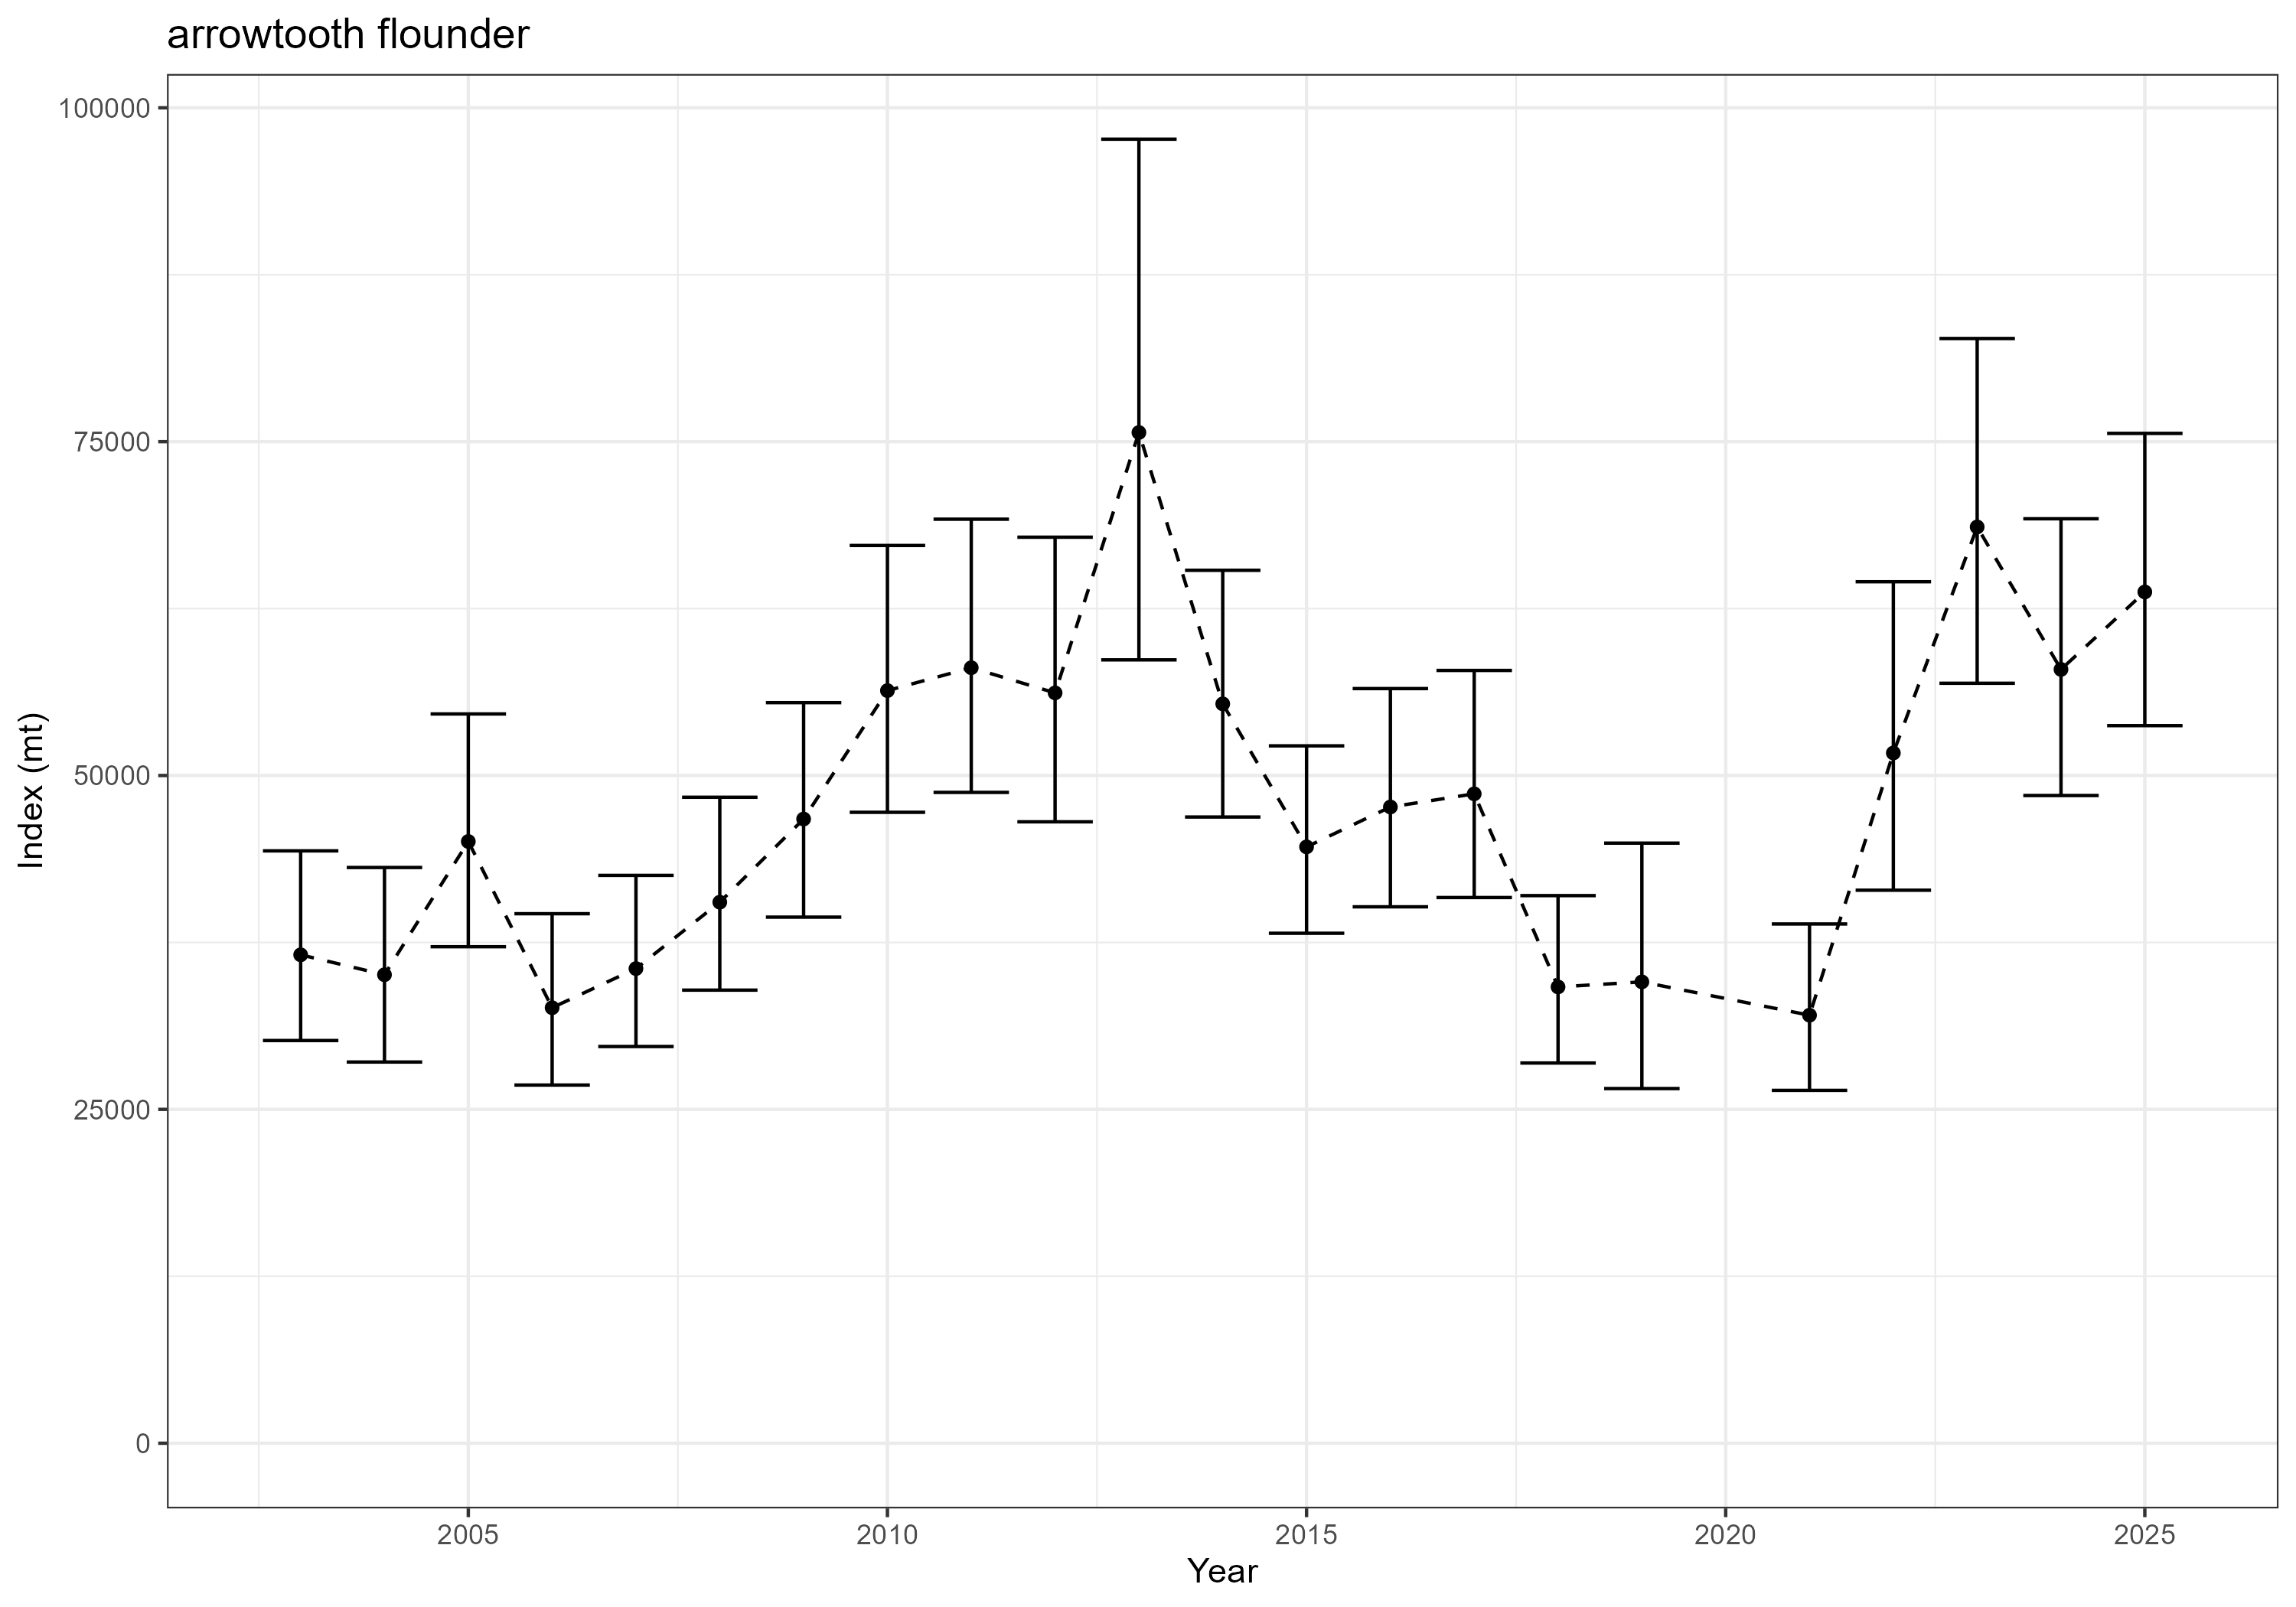
\includegraphics[width=0.95\linewidth,height=\textheight,keepaspectratio]{../plots/wcgbts_indices/arrowtooth_flounder_index.png}

}

\caption{Estimated relative index of abundance for arrowtooth flounder
from the NWFSC WCGBTS.}

\end{figure}%

\begin{figure}[H]

{\centering 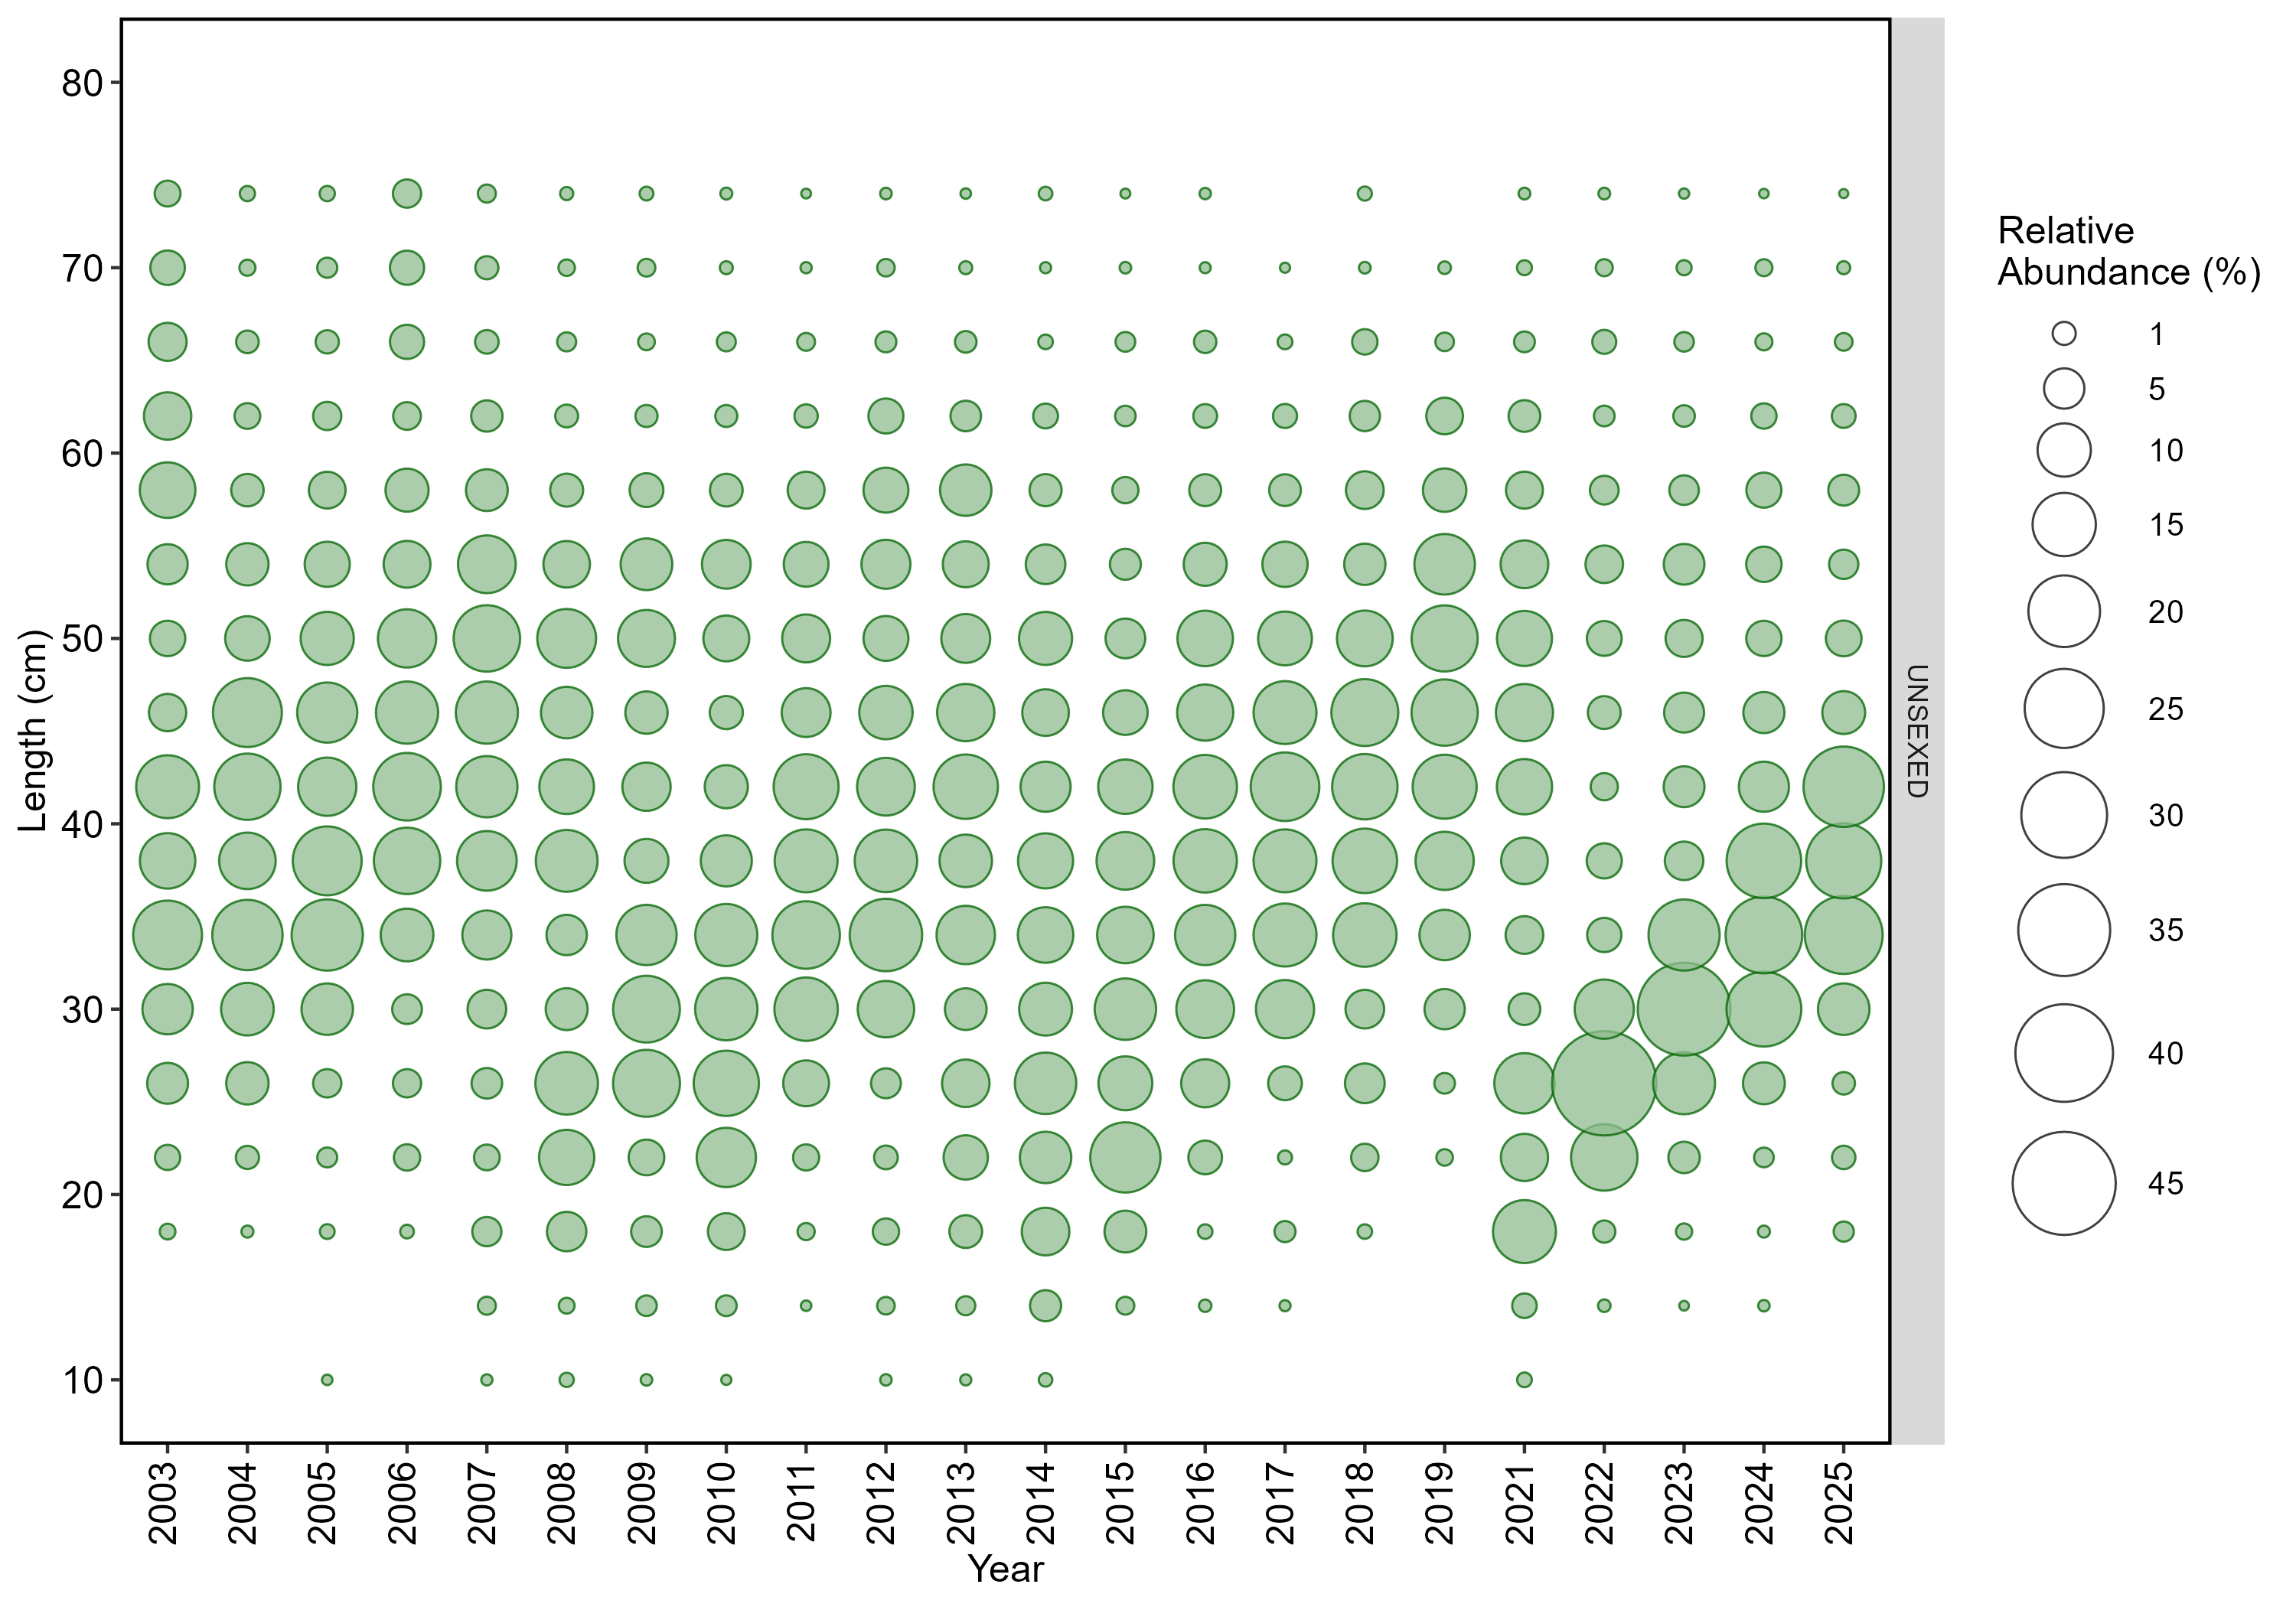
\includegraphics[width=0.95\linewidth,height=\textheight,keepaspectratio]{../plots/wcgbts_comps/plots/arrowtooth flounder_length_frequency_sex_0.png}

}

\caption{Length (cm) compostion data from the NWFSC WCGBTS for
arrowtooth flounder. Size of the circles within a year indicate higher
(larger circles) and lower (smaller circles) proportion observed by
length bin.}

\end{figure}%

\newpage{}

\newpage{}

\subsection{Aurora rockfish}\label{aurora-rockfish}

The most recent assessment of aurora rockfish was a benchmark assessment
conducted in 2013. Across available data, aurora rockfish have been
observed and sampled by the NWFSC WCGBTS. The NWFSC WCGBTS observed
aurora rockfish on an average of 84 tows per year. For this species, a
total of 617 maturity samples have been collected coastwide (regardless
of stock area), with 567 read maturities.

\begingroup\fontsize{10}{12}\selectfont
\begingroup\fontsize{10}{12}\selectfont

\begin{longtable}[t]{>{\raggedleft\arraybackslash}p{2cm}>{\raggedleft\arraybackslash}p{3.5cm}>{\raggedleft\arraybackslash}p{2cm}>{\raggedleft\arraybackslash}p{2cm}>{\raggedleft\arraybackslash}p{2cm}}
\caption{\label{tab:unnamed-chunk-20}Total number of available lengths, read ages, and unread age structures by data source and
state for aurora rockfish.}\\
\toprule
State & Source & Lengths & Ages & Age Structures\\
\midrule
\endfirsthead
\caption[]{Total number of available lengths, read ages, and unread age structures by data source and
state for aurora rockfish. (\textit{continued)}}\\
\toprule
State & Source & Lengths & Ages & Age Structures\\
\midrule
\endhead

\endfoot
\bottomrule
\endlastfoot
CA & NWFSC WCGBTS & 26,965 & 2,269 & 8,409\\
OR & NWFSC WCGBTS & 5,688 & 784 & 3,009\\
WA & NWFSC WCGBTS & 384 & 37 & 258\\*
\end{longtable}
\endgroup{}
\endgroup{}

\begin{figure}[H]

{\centering 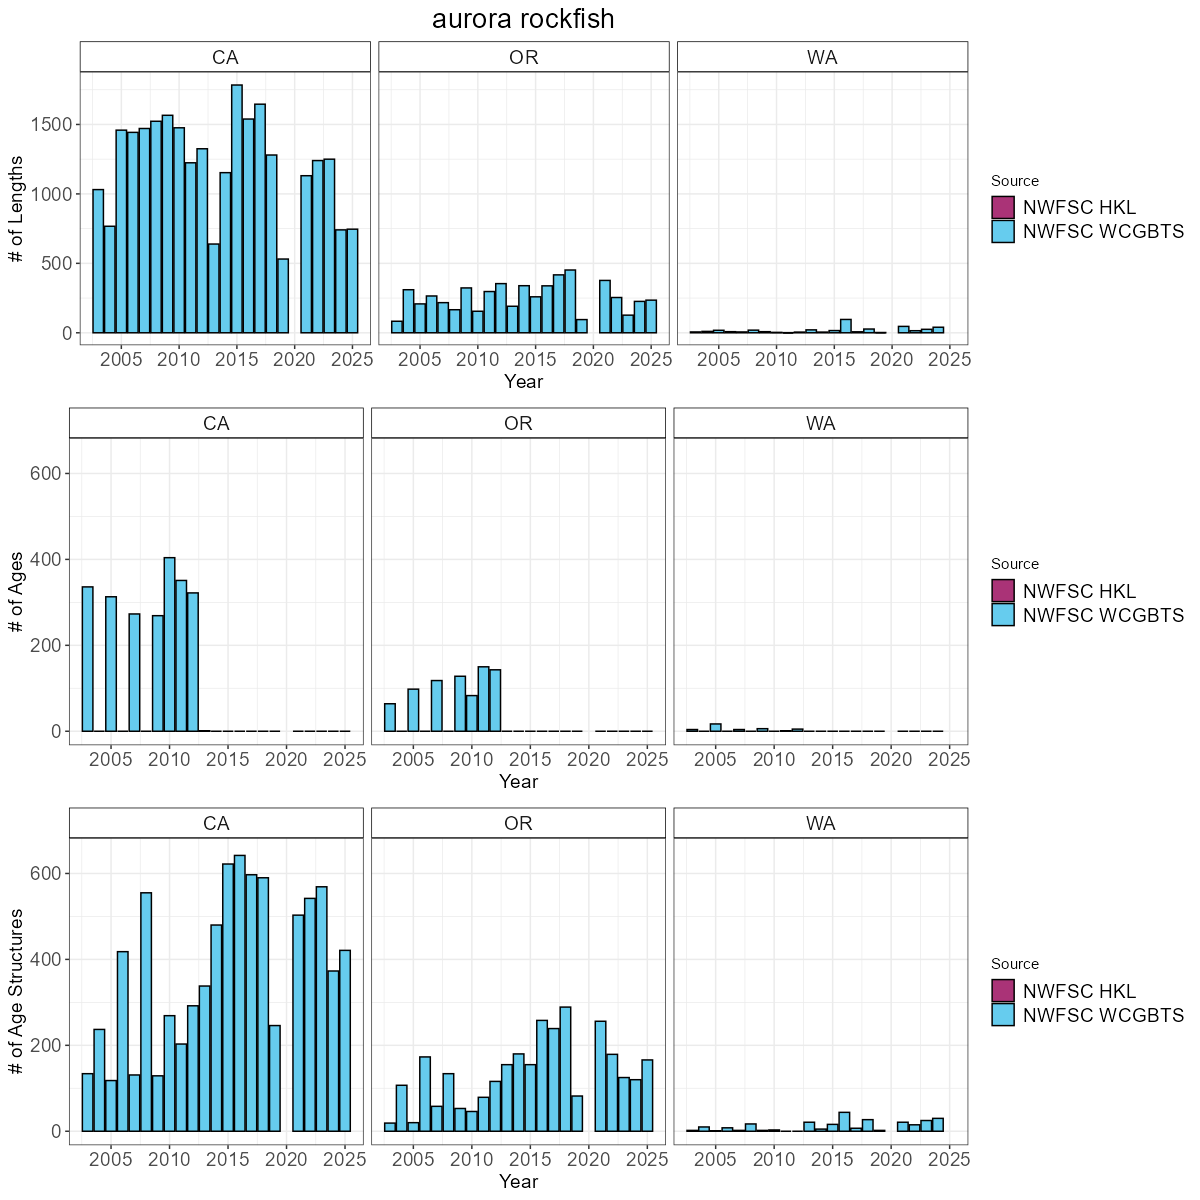
\includegraphics[width=0.95\linewidth,height=\textheight,keepaspectratio]{../plots/state_comparisons/aurora_rockfish_state_compositions.png}

}

\caption{Total number of available lengths, read ages, and unread age
structures by data source by year for aurora rockfish. Note the y-axis
maximum may differ by data type.}

\end{figure}%

\begin{figure}[H]

{\centering 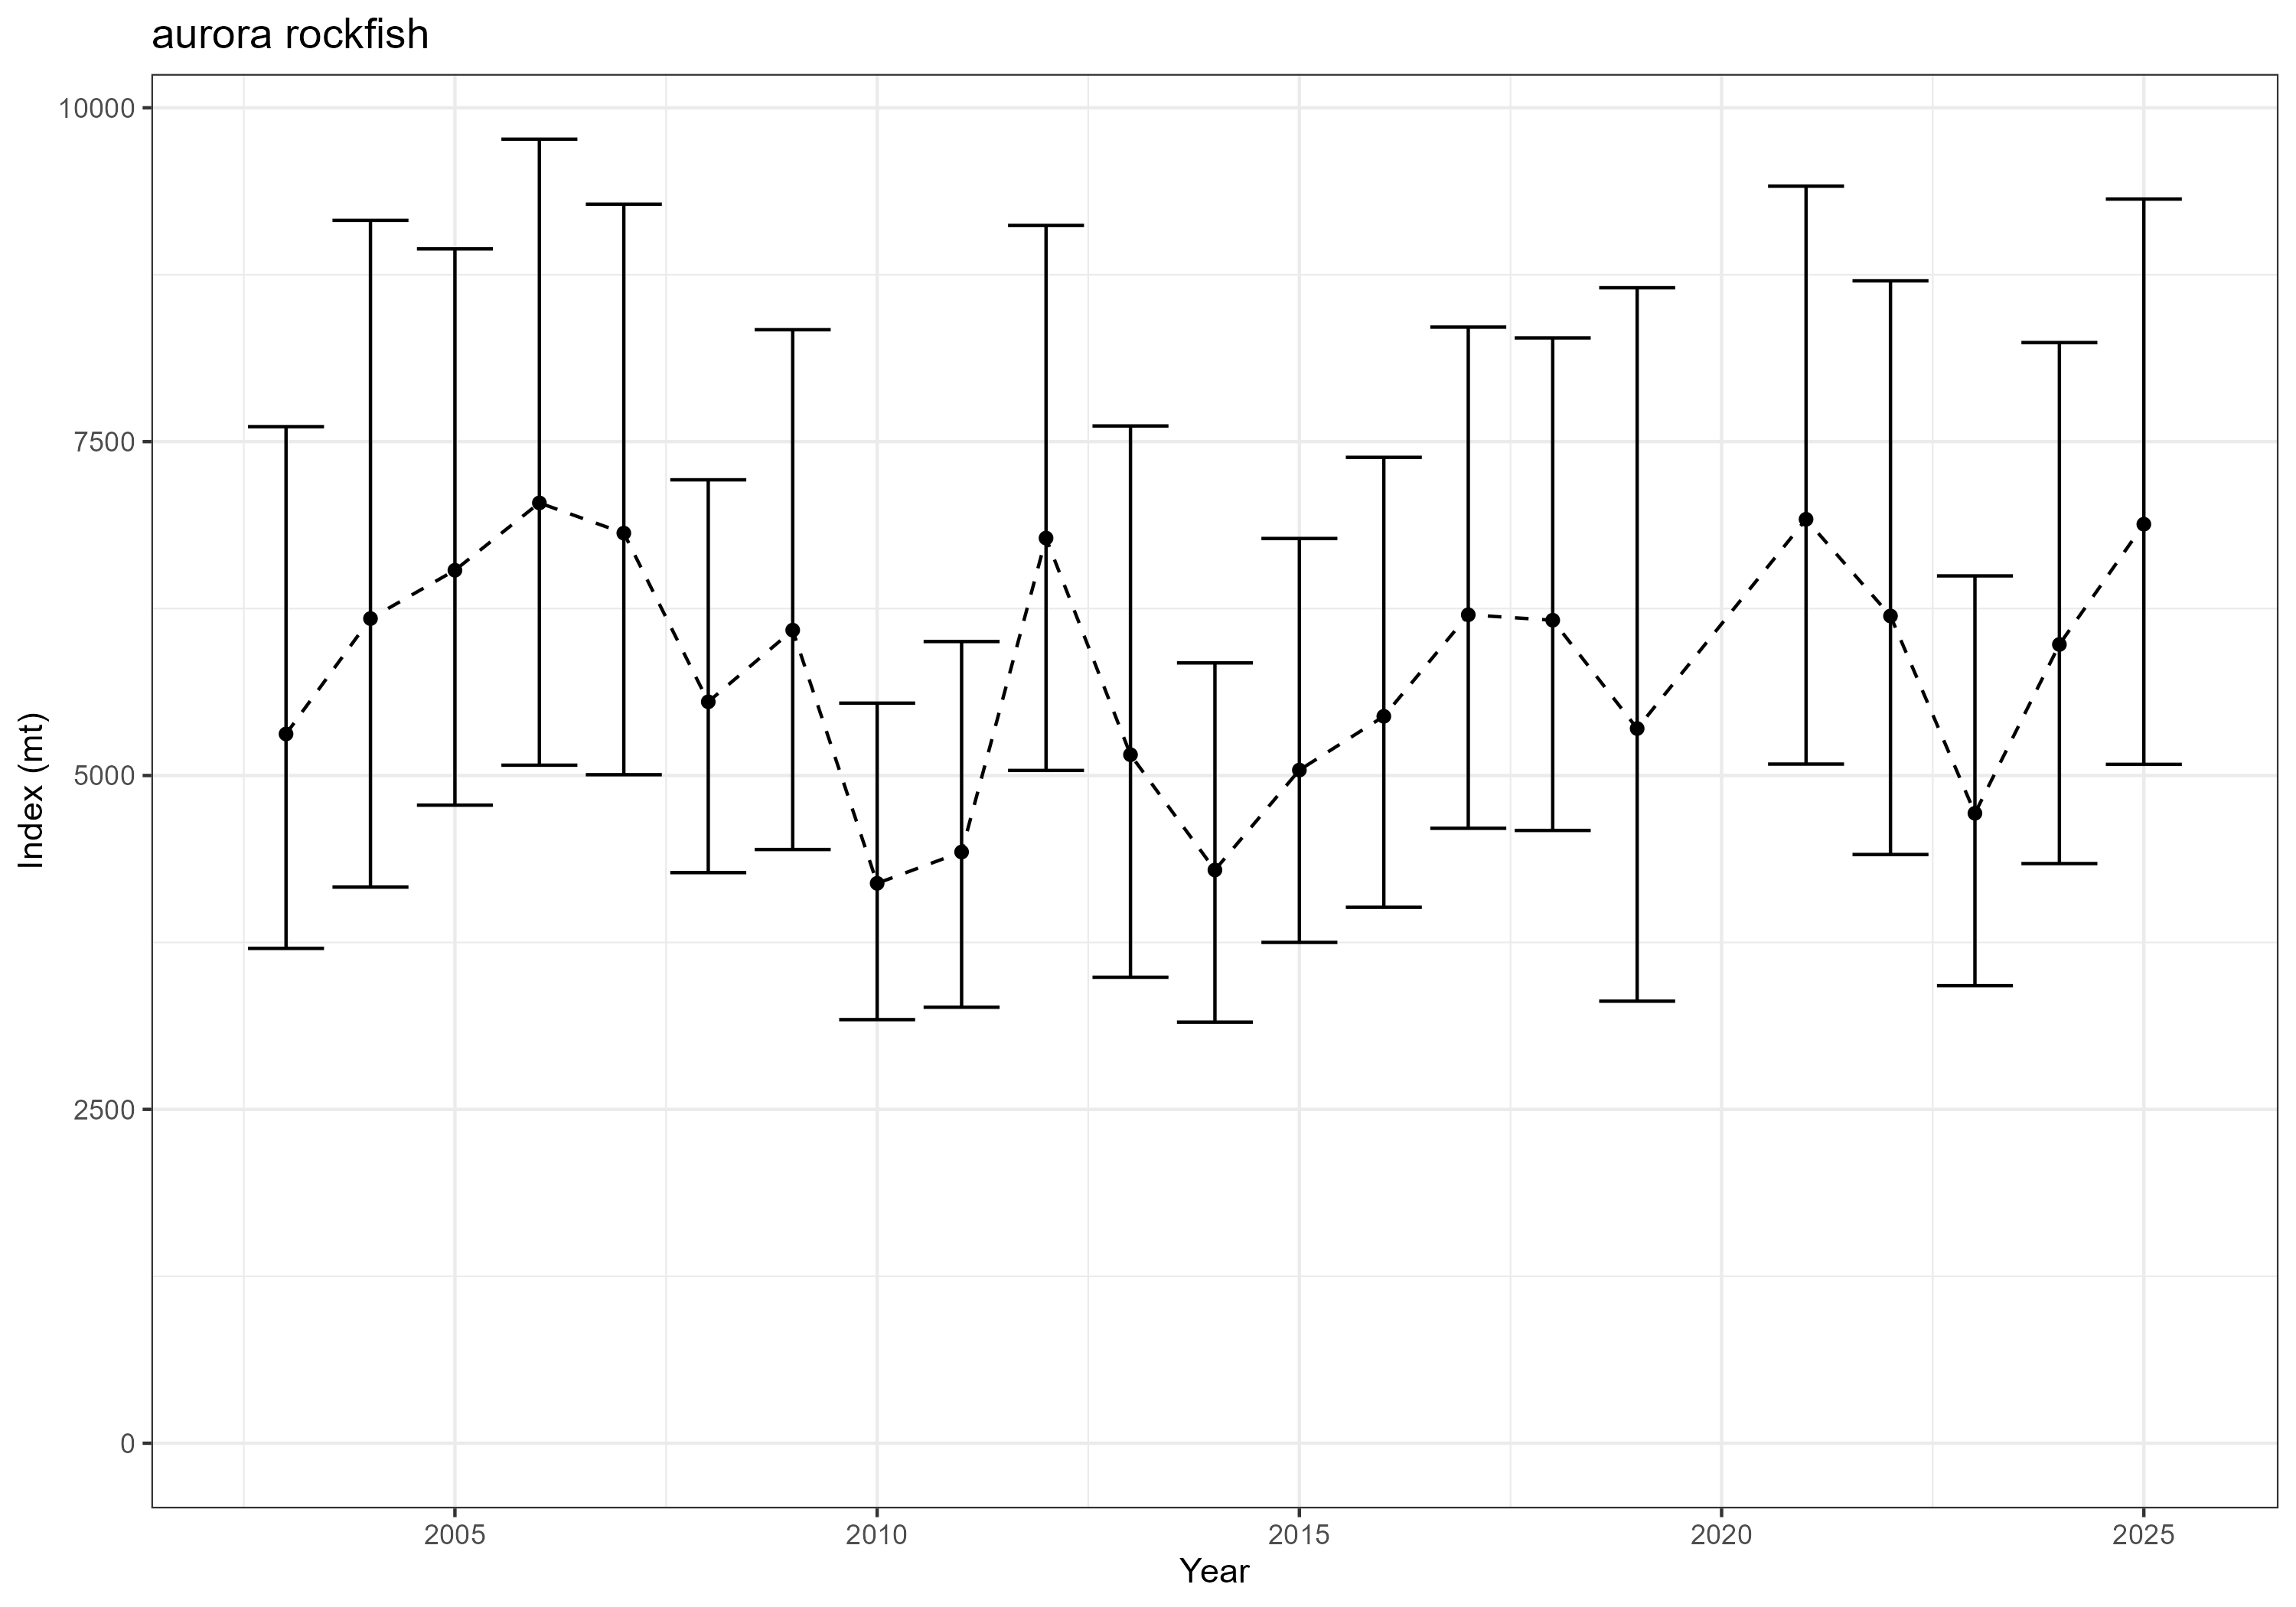
\includegraphics[width=0.95\linewidth,height=\textheight,keepaspectratio]{../plots/wcgbts_indices/aurora_rockfish_index.png}

}

\caption{Estimated relative index of abundance for aurora rockfish from
the NWFSC WCGBTS.}

\end{figure}%

\begin{figure}[H]

{\centering 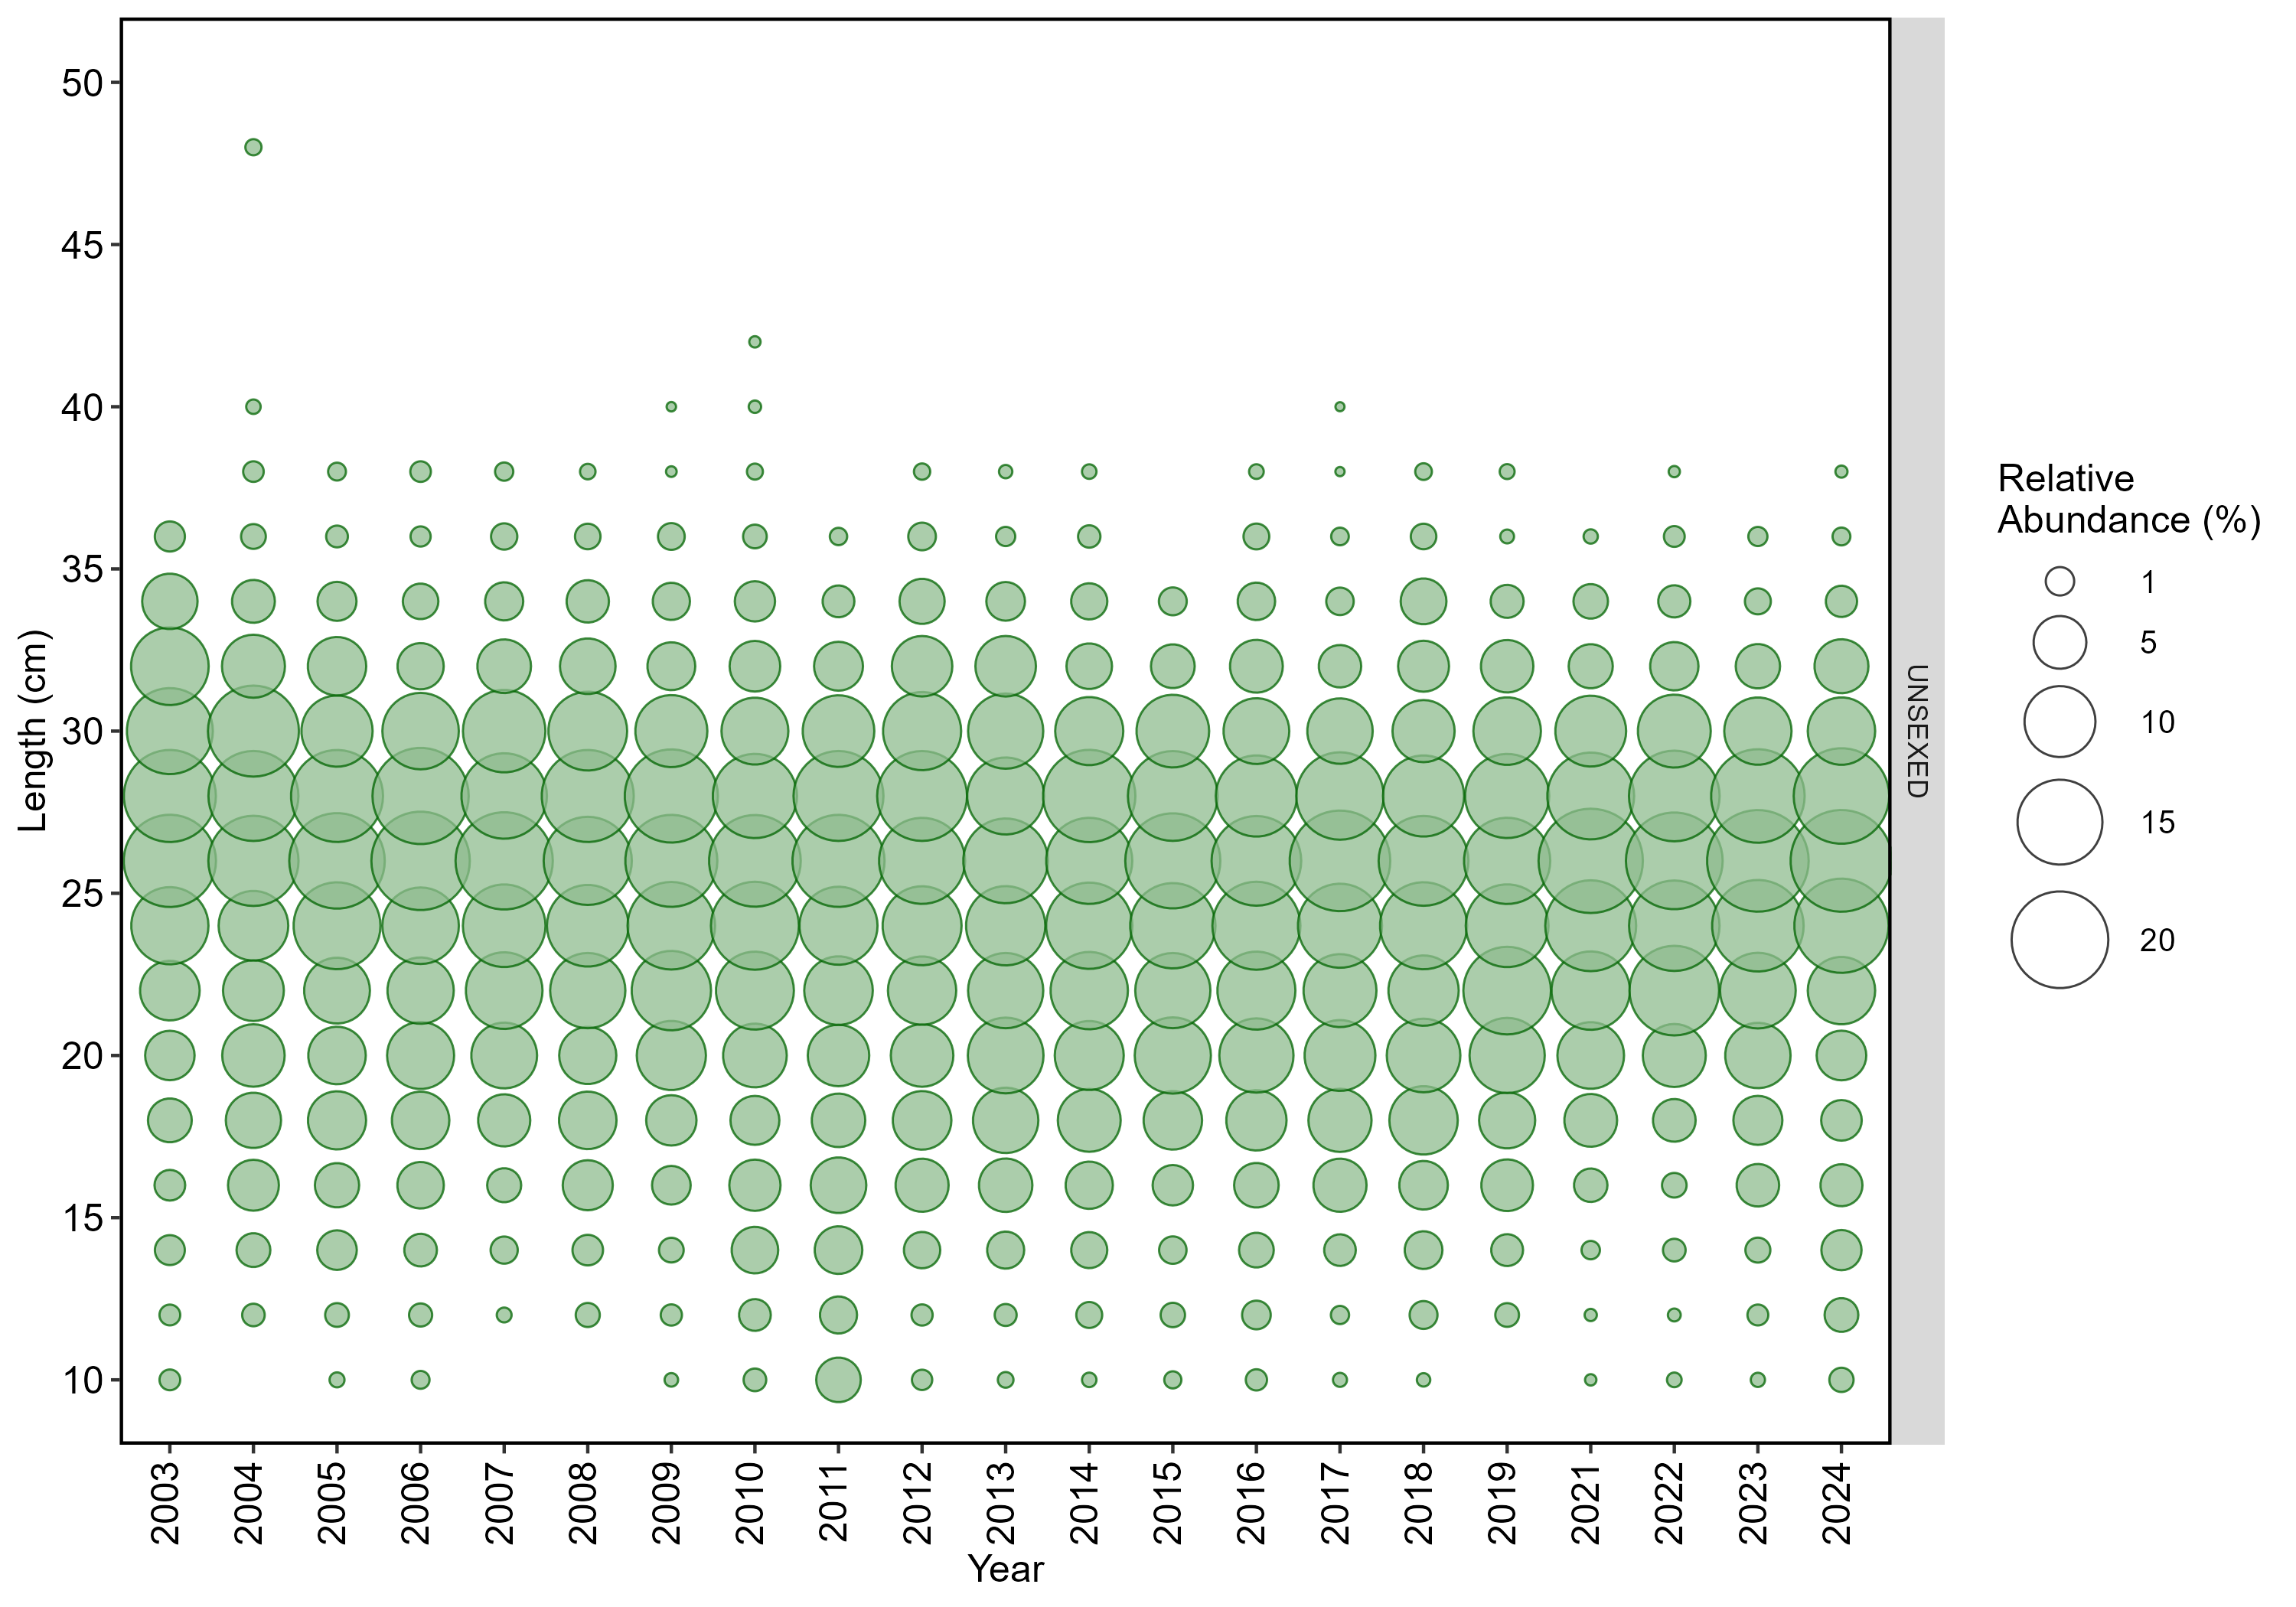
\includegraphics[width=0.95\linewidth,height=\textheight,keepaspectratio]{../plots/wcgbts_comps/plots/aurora rockfish_length_frequency_sex_0.png}

}

\caption{Length (cm) compostion data from the NWFSC WCGBTS for aurora
rockfish. Size of the circles within a year indicate higher (larger
circles) and lower (smaller circles) proportion observed by length bin.}

\end{figure}%

\newpage{}

\subsection{Bank rockfish}\label{bank-rockfish}

To date, no assessment or analysis has been conducted on bank rockfish.
Across available data, bank rockfish have been observed and sampled by
both the NWFSC HKLS and WCGBTS. The NWFSC HKLS observed bank rockfish at
an average of 30 sets per year. The NWFSC WCGBTS observed bank rockfish
on an average of 13 tows per year. For this species, a total of 733
maturity samples have been collected coastwide (regardless of stock
area), with 85 read maturities.

\begingroup\fontsize{10}{12}\selectfont
\begingroup\fontsize{10}{12}\selectfont

\begin{longtable}[t]{>{\raggedleft\arraybackslash}p{2cm}>{\raggedleft\arraybackslash}p{3.5cm}>{\raggedleft\arraybackslash}p{2cm}>{\raggedleft\arraybackslash}p{2cm}>{\raggedleft\arraybackslash}p{2cm}}
\caption{\label{tab:unnamed-chunk-37}Total number of available lengths, read ages, and unread age structures by data source and
state for bank rockfish.}\\
\toprule
State & Source & Lengths & Ages & Age Structures\\
\midrule
\endfirsthead
\caption[]{Total number of available lengths, read ages, and unread age structures by data source and
state for bank rockfish. (\textit{continued)}}\\
\toprule
State & Source & Lengths & Ages & Age Structures\\
\midrule
\endhead

\endfoot
\bottomrule
\endlastfoot
CA & NWFSC HKLS & 3,952 & 0 & 3,936\\
CA & NWFSC WCGBTS & 2,236 & 0 & 1,571\\
OR & NWFSC WCGBTS & 143 & 0 & 56\\
WA & NWFSC WCGBTS & 4 & 0 & 4\\*
\end{longtable}
\endgroup{}
\endgroup{}

\begin{figure}[H]

{\centering 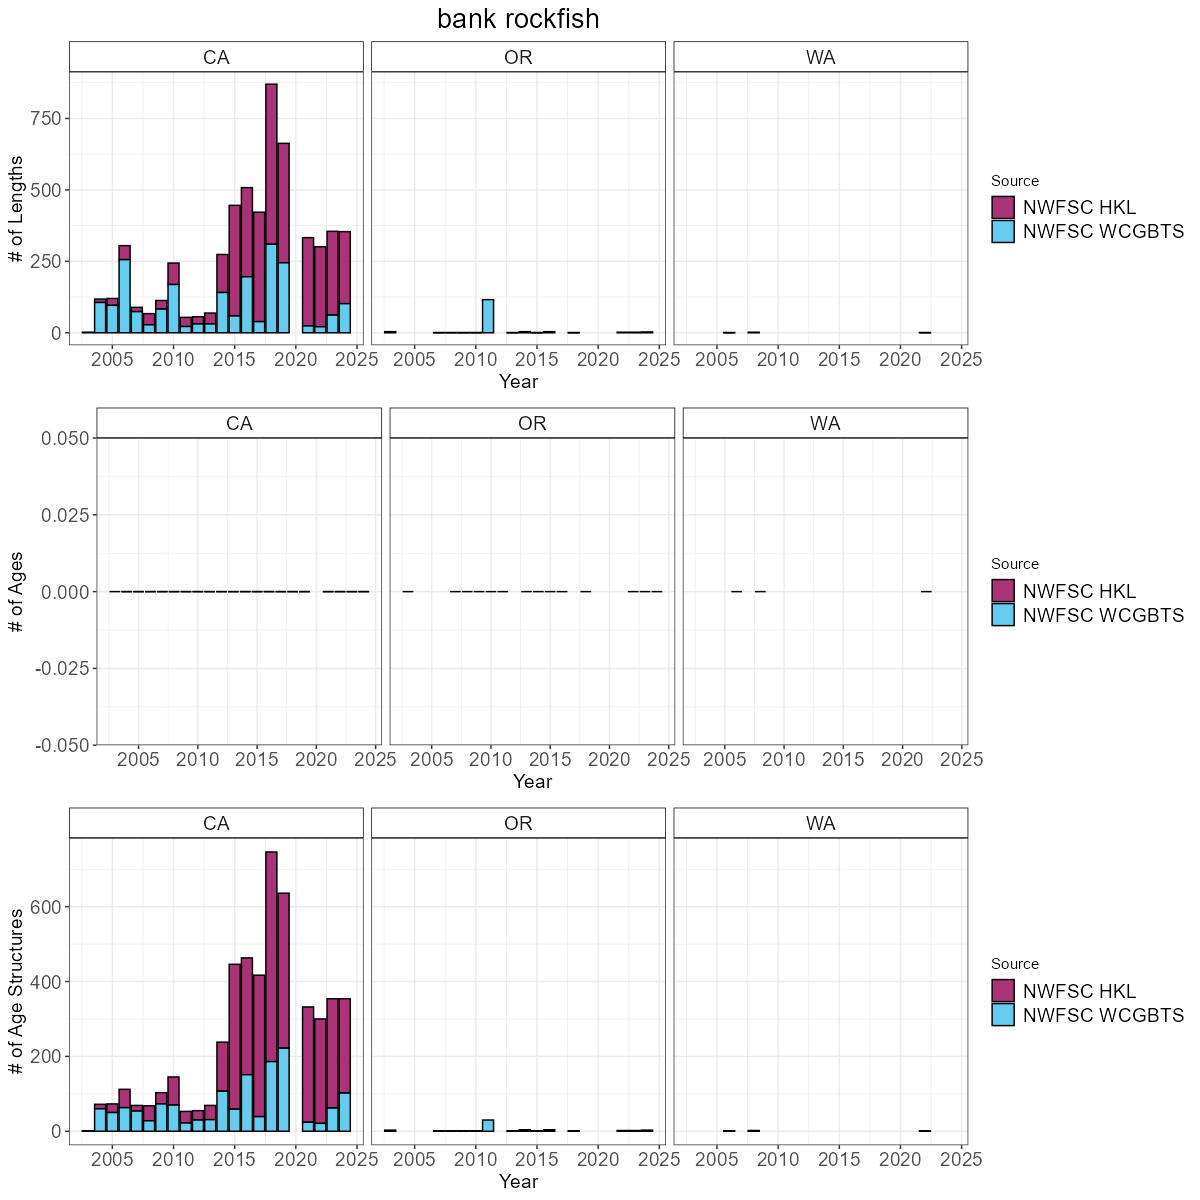
\includegraphics[width=0.95\linewidth,height=\textheight,keepaspectratio]{../plots/state_comparisons/bank_rockfish_state_compositions.png}

}

\caption{Total number of available lengths, read ages, and unread age
structures by data source by year for bank rockfish. Note the y-axis
maximum may differ by data type.}

\end{figure}%

\begin{figure}[H]

{\centering 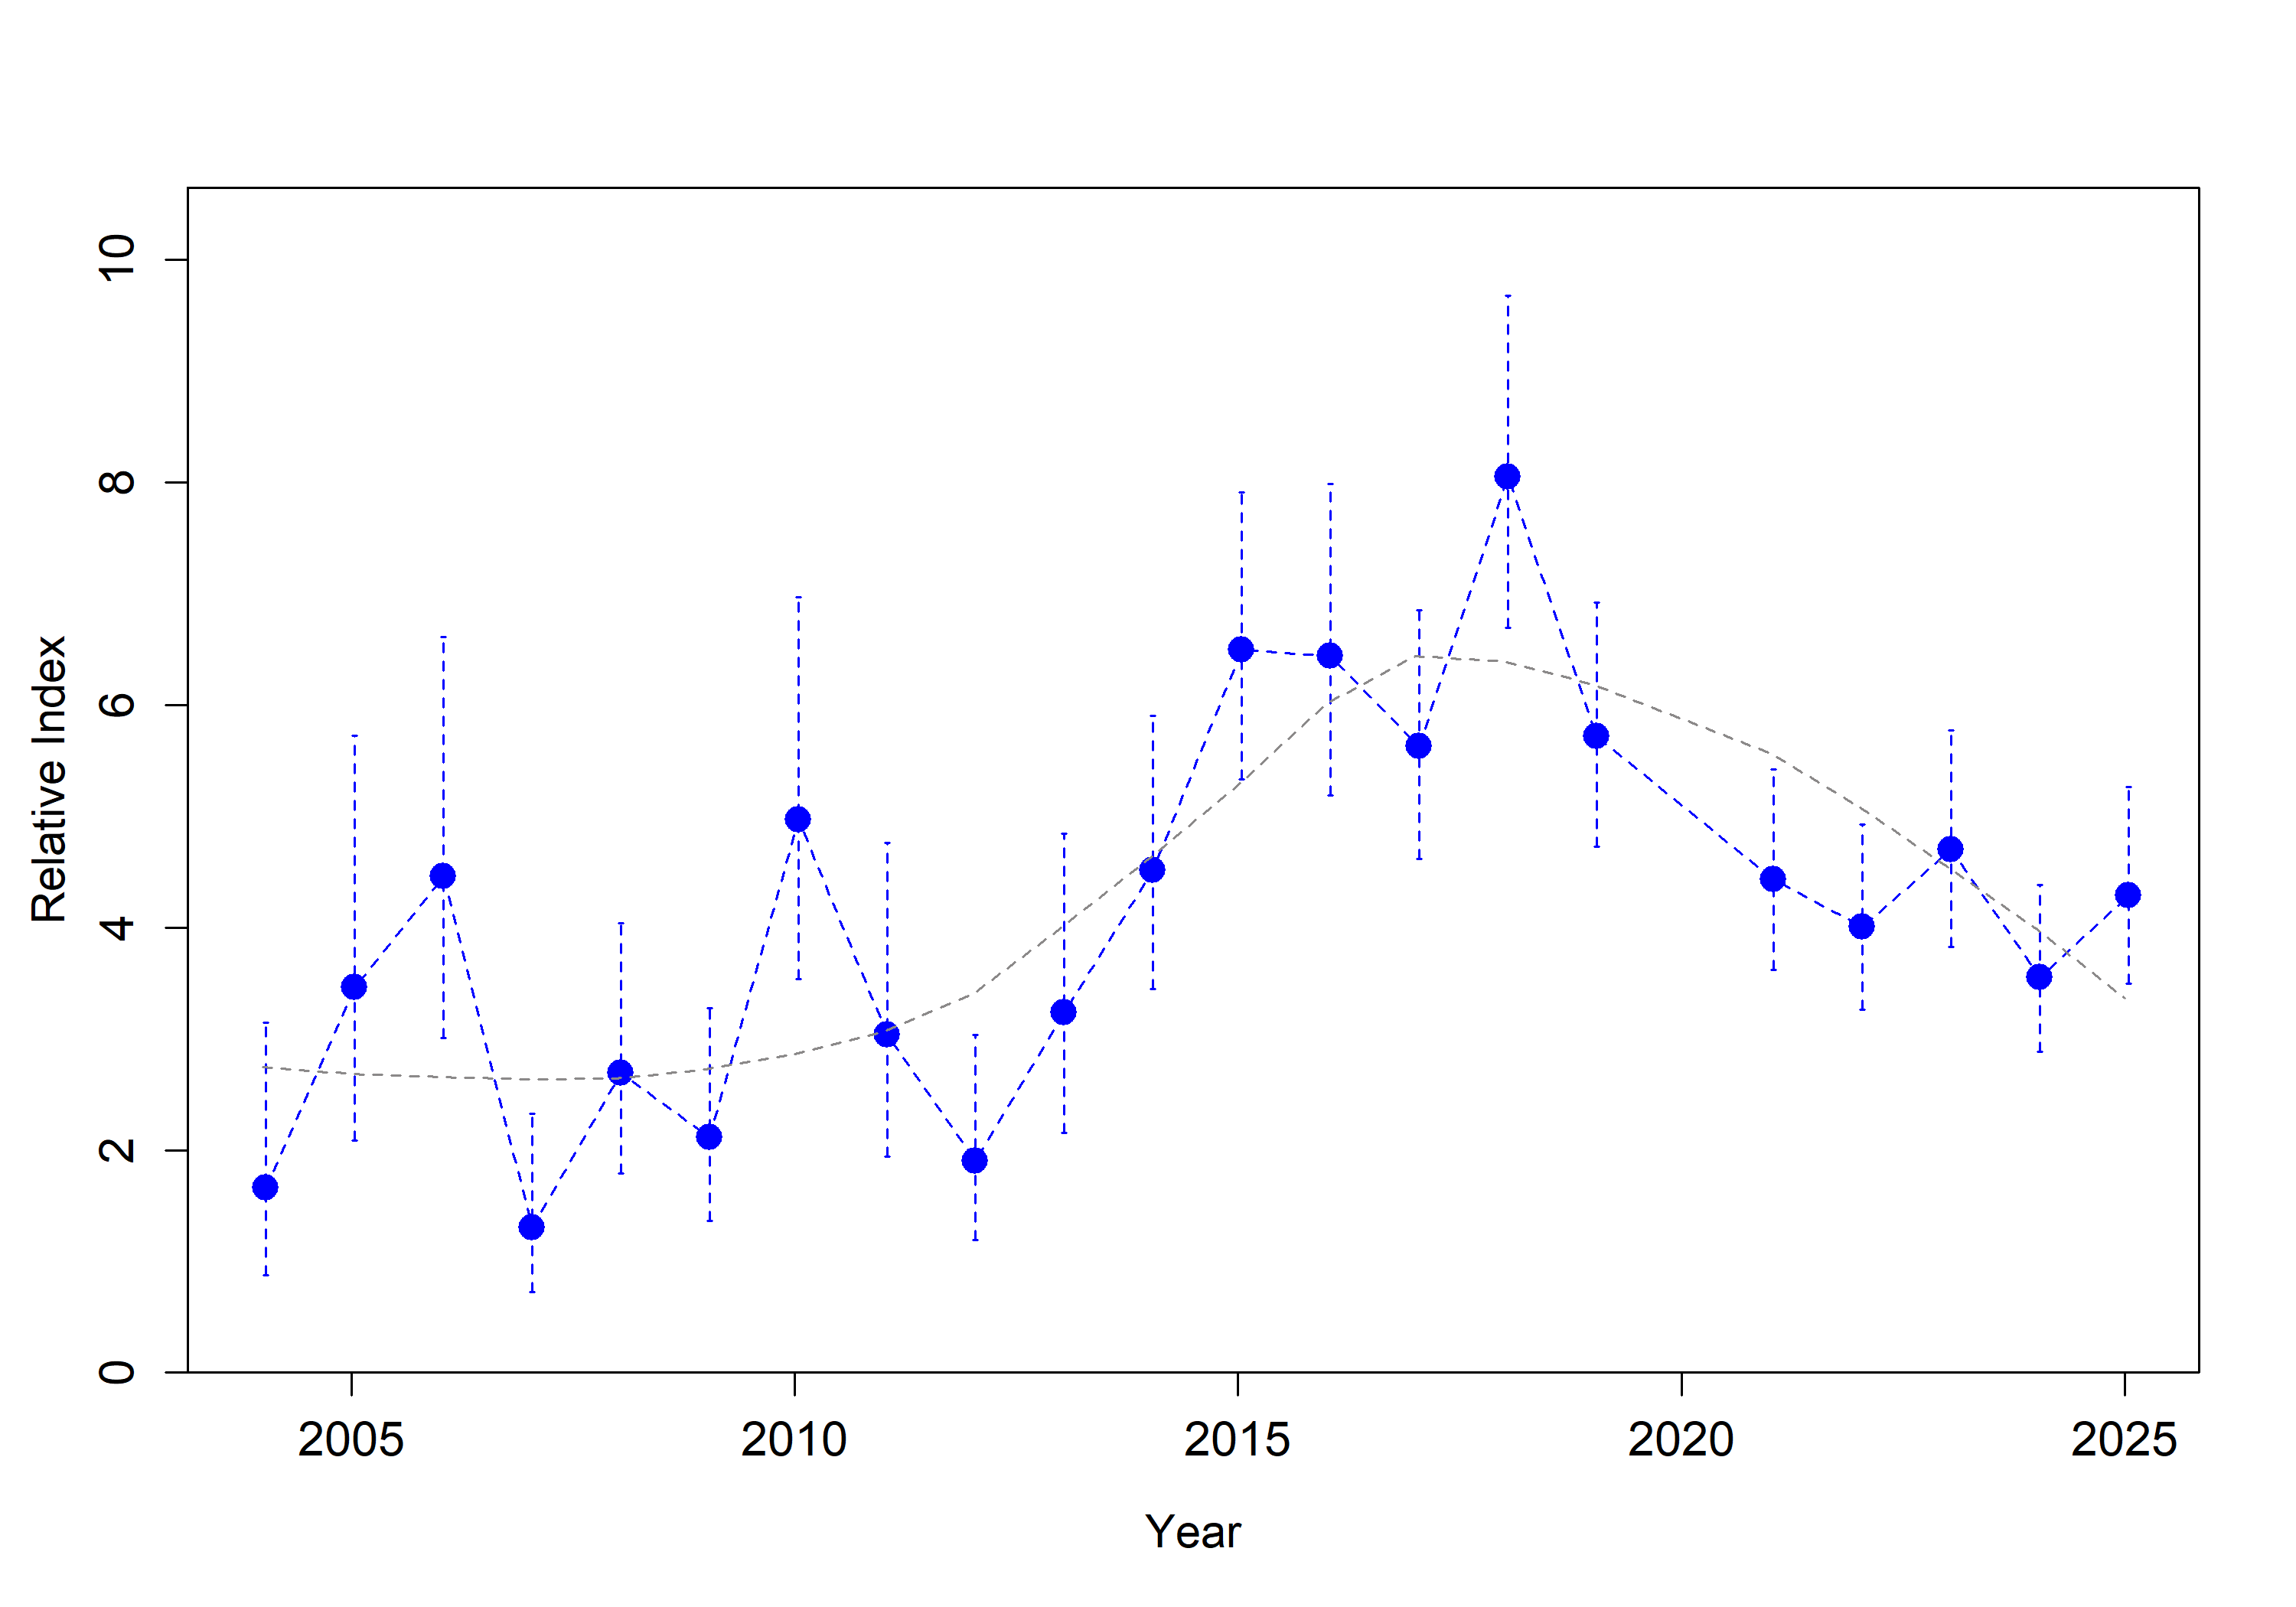
\includegraphics[width=0.95\linewidth,height=\textheight,keepaspectratio]{../plots/hkl_indices/bank rockfish_negbinom index.png}

}

\caption{Estimated relative index of abundance for bank rockfish from
the NWFSC HKLS.}

\end{figure}%

\begin{figure}[H]

{\centering 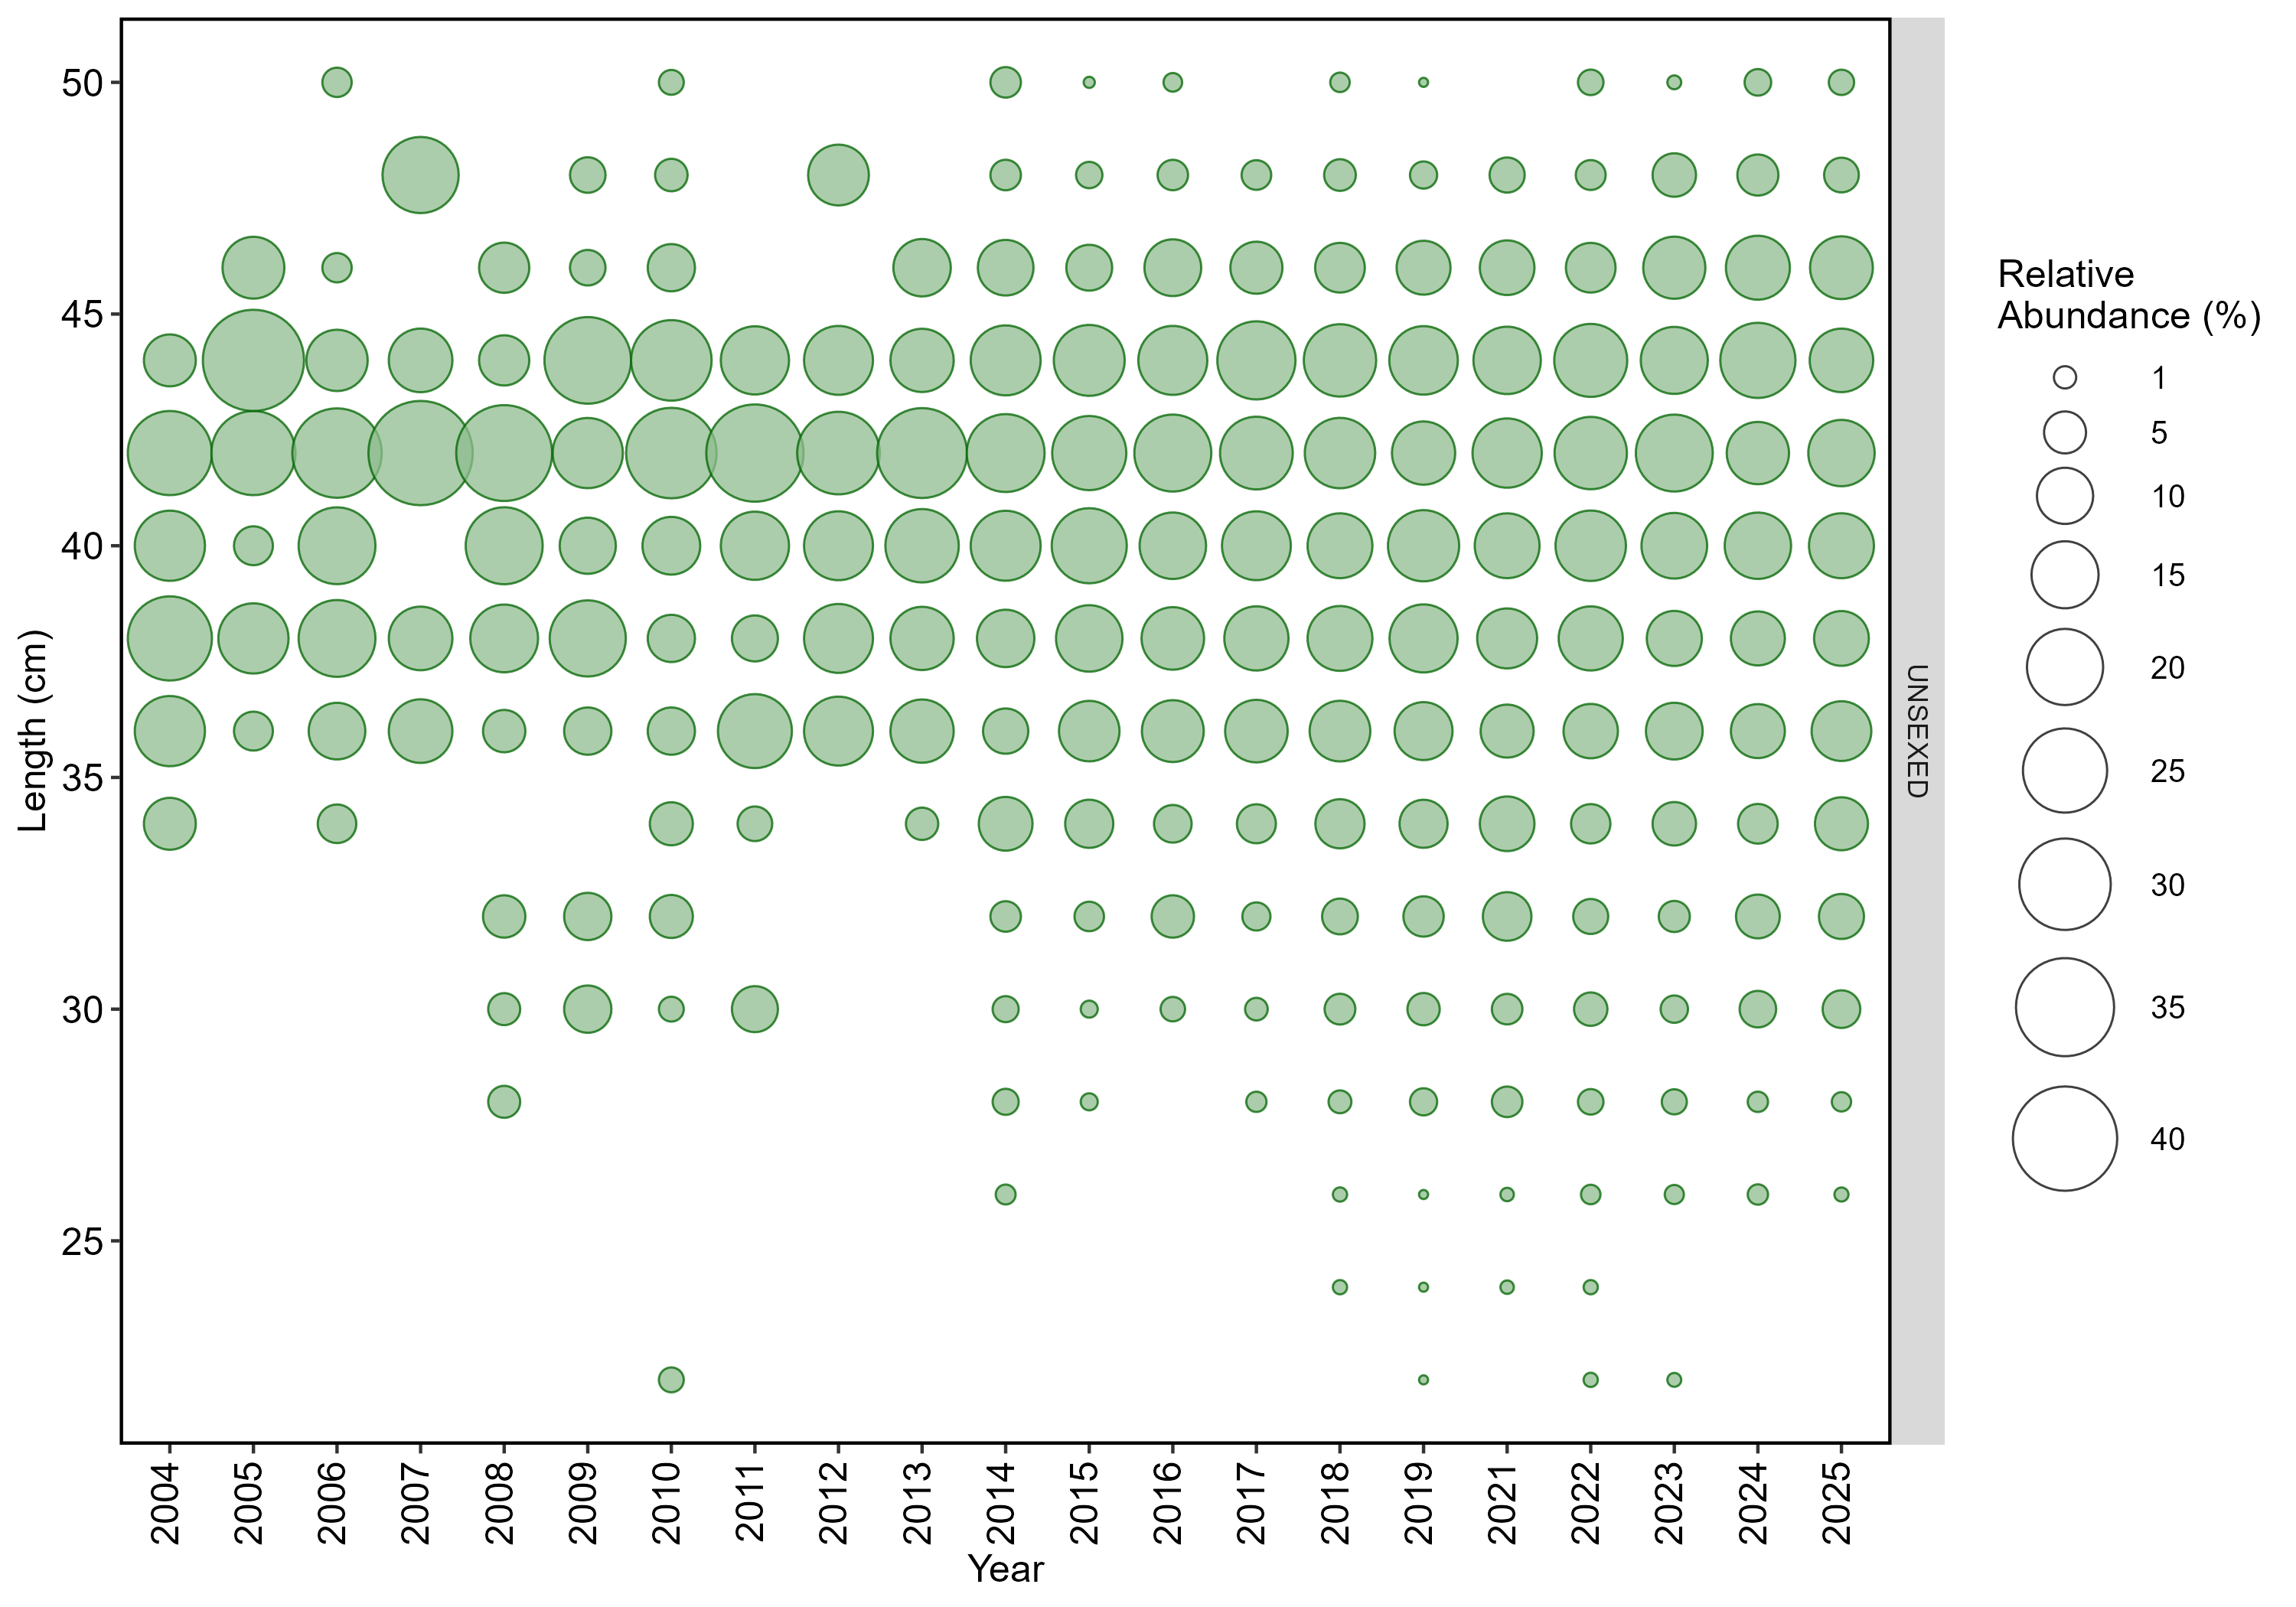
\includegraphics[width=0.95\linewidth,height=\textheight,keepaspectratio]{../plots/hkl_comps/plots/bank rockfish_nwfsc_hkl_length_frequency_sex_0.png}

}

\caption{Length (cm) compostion data from the NWFSC HKLS for bank
rockfish. Size of the circles within a year indicate higher (larger
circles) and lower (smaller circles) proportion observed by length bin.}

\end{figure}%

\newpage{}

\subsection{Big skate}\label{big-skate}

The most recent assessment of big skate was a benchmark assessment
conducted in 2019. Across available data, big skate have been observed
and sampled by the NWFSC WCGBTS. The NWFSC WCGBTS observed big skate on
an average of 96 tows per year. For this species, a total of 180
maturity samples have been collected coastwide (regardless of stock
area), with 180 read maturities.

\begingroup\fontsize{10}{12}\selectfont
\begingroup\fontsize{10}{12}\selectfont

\begin{longtable}[t]{>{\raggedleft\arraybackslash}p{2cm}>{\raggedleft\arraybackslash}p{3.5cm}>{\raggedleft\arraybackslash}p{2cm}>{\raggedleft\arraybackslash}p{2cm}>{\raggedleft\arraybackslash}p{2cm}}
\caption{\label{tab:unnamed-chunk-54}Total number of available lengths, read ages, and unread age structures by data source and
state for big skate.}\\
\toprule
State & Source & Lengths & Ages & Age Structures\\
\midrule
\endfirsthead
\caption[]{Total number of available lengths, read ages, and unread age structures by data source and
state for big skate. (\textit{continued)}}\\
\toprule
State & Source & Lengths & Ages & Age Structures\\
\midrule
\endhead

\endfoot
\bottomrule
\endlastfoot
CA & NWFSC WCGBTS & 2,339 & 351 & 182\\
OR & NWFSC WCGBTS & 2,719 & 422 & 369\\
WA & NWFSC WCGBTS & 2,023 & 261 & 261\\*
\end{longtable}
\endgroup{}
\endgroup{}

\begin{figure}[H]

{\centering 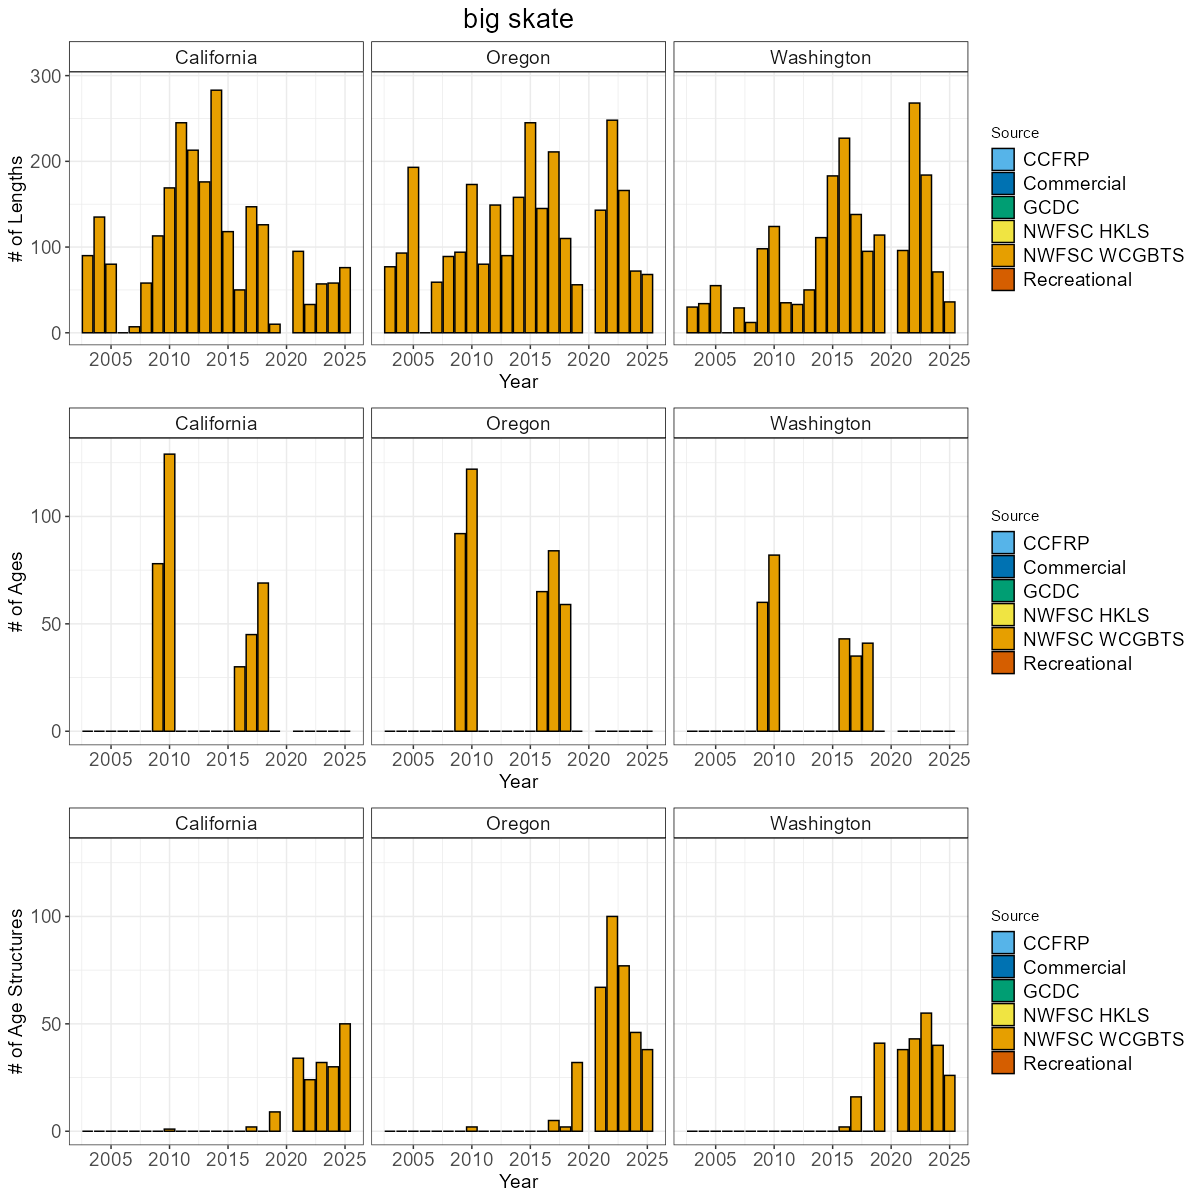
\includegraphics[width=0.95\linewidth,height=\textheight,keepaspectratio]{../plots/state_comparisons/big_skate_state_compositions.png}

}

\caption{Total number of available lengths, read ages, and unread age
structures by data source by year for big skate. Note the y-axis maximum
may differ by data type.}

\end{figure}%

\begin{figure}[H]

{\centering 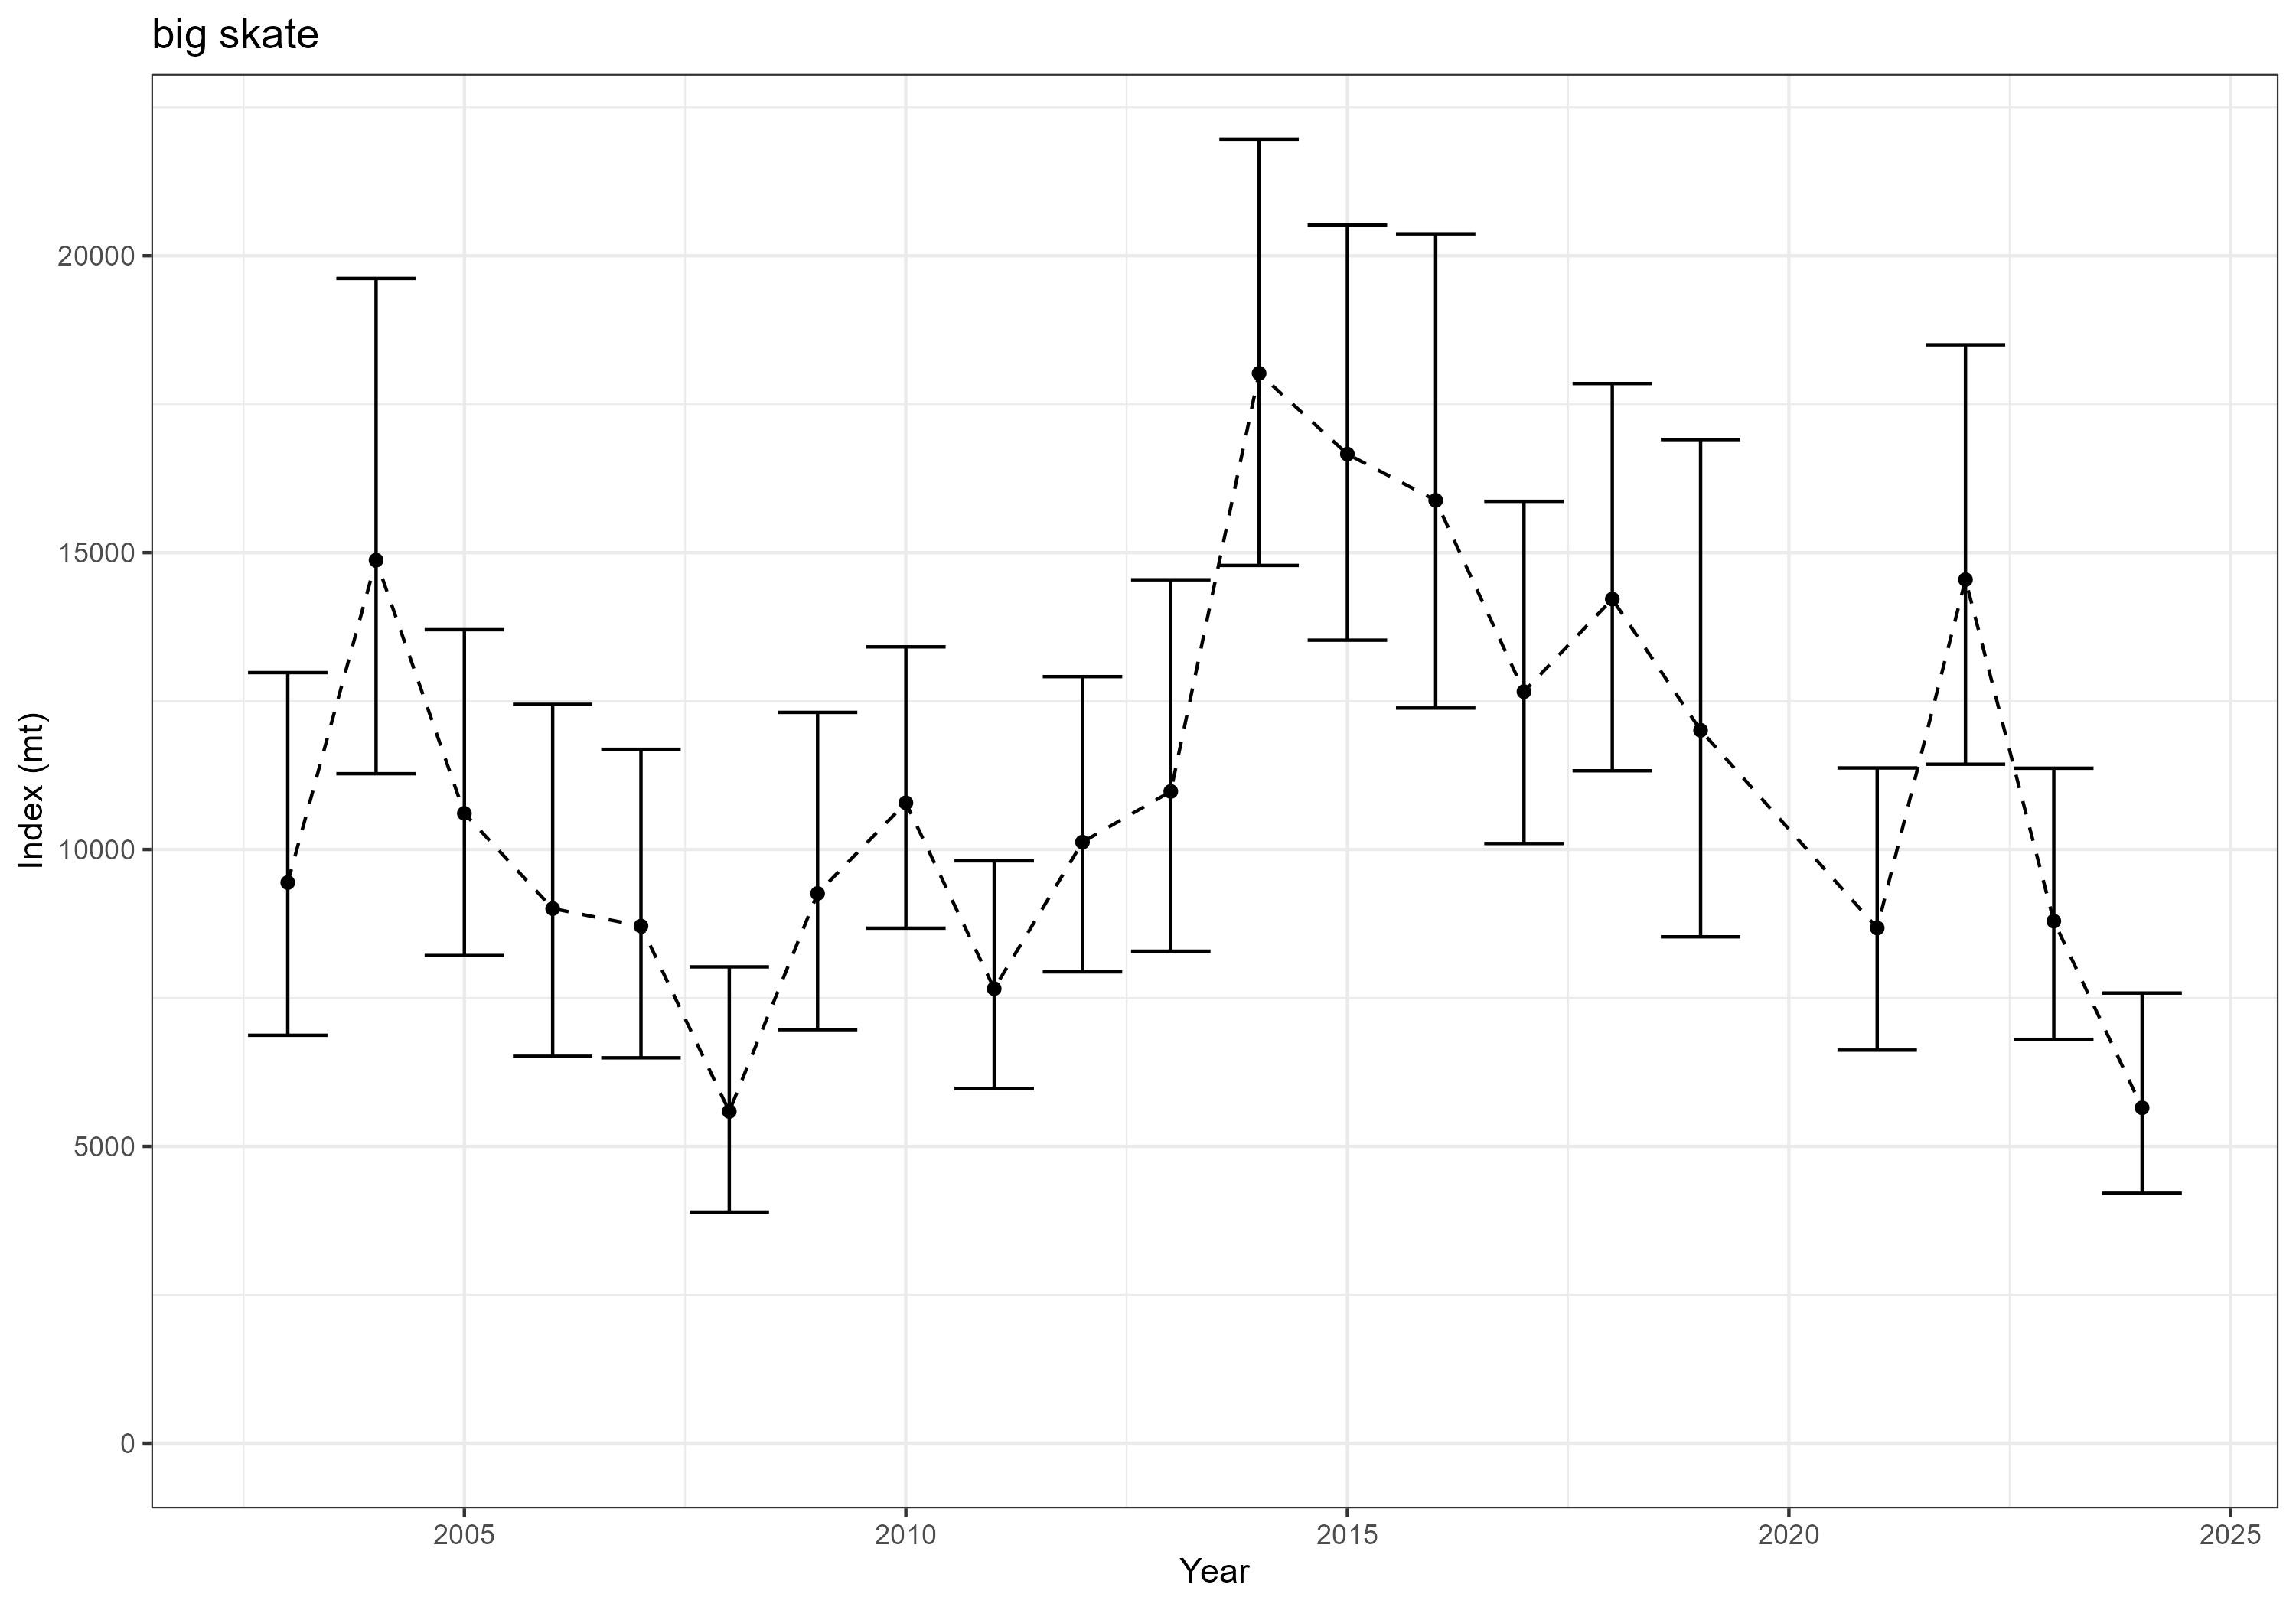
\includegraphics[width=0.95\linewidth,height=\textheight,keepaspectratio]{../plots/wcgbts_indices/big_skate_index.png}

}

\caption{Estimated relative index of abundance for big skate from the
NWFSC WCGBTS.}

\end{figure}%

\begin{figure}[H]

{\centering 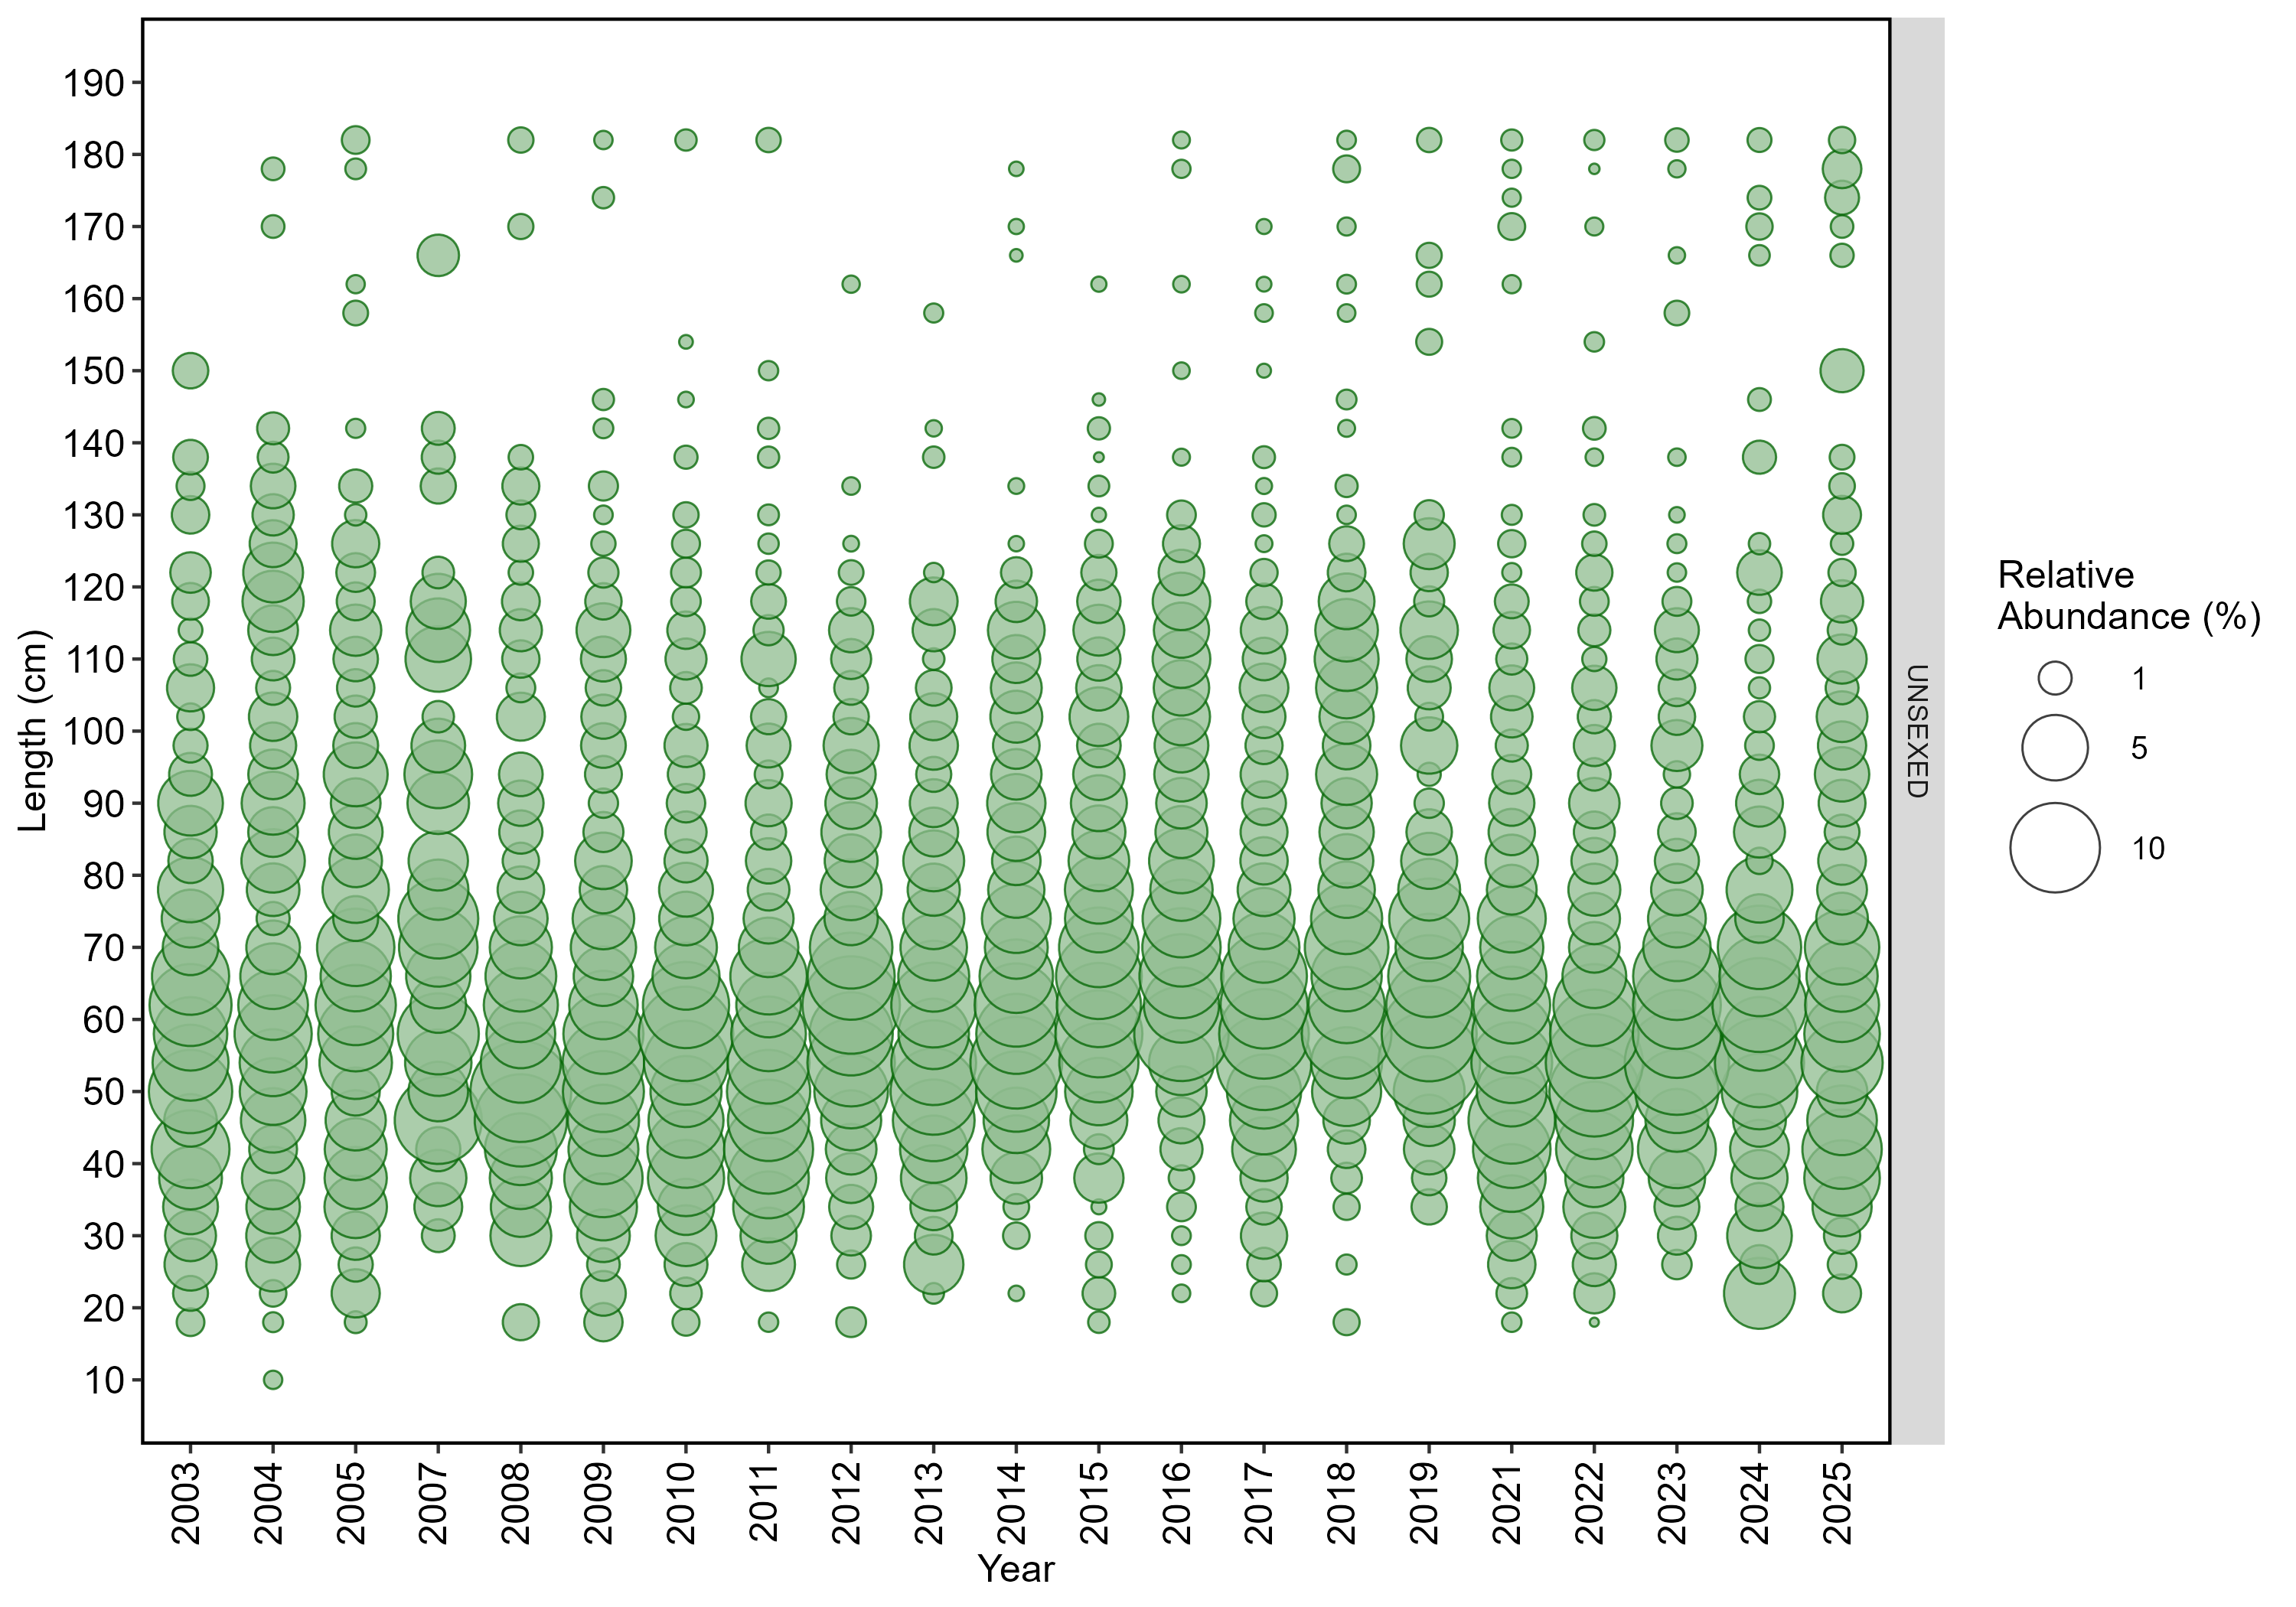
\includegraphics[width=0.95\linewidth,height=\textheight,keepaspectratio]{../plots/additional_wcgbts_comps/plots/big skate_length_frequency_sex_0.png}

}

\caption{Length (cm) compostion data from the NWFSC WCGBTS for big
skate. Size of the circles within a year indicate higher (larger
circles) and lower (smaller circles) proportion observed by length bin.}

\end{figure}%

\newpage{}

\subsection{Blackgill rockfish}\label{blackgill-rockfish}

The most recent assessment of blackgill rockfish was an update
assessment conducted in 2017. Across available data, blackgill rockfish
have been observed and sampled by both the NWFSC HKLS and WCGBTS. The
NWFSC HKLS observed blackgill rockfish at an average of 0 sets per year.
The NWFSC WCGBTS observed blackgill rockfish on an average of 35 tows
per year. For this species, a total of 126 maturity samples have been
collected coastwide (regardless of stock area), with 126 read
maturities.

\begingroup\fontsize{10}{12}\selectfont
\begingroup\fontsize{10}{12}\selectfont

\begin{longtable}[t]{>{\raggedleft\arraybackslash}p{2cm}>{\raggedleft\arraybackslash}p{3.5cm}>{\raggedleft\arraybackslash}p{2cm}>{\raggedleft\arraybackslash}p{2cm}>{\raggedleft\arraybackslash}p{2cm}}
\caption{\label{tab:unnamed-chunk-72}Total number of available lengths, read ages, and unread age structures by data source and
state for blackgill rockfish.}\\
\toprule
State & Source & Lengths & Ages & Age Structures\\
\midrule
\endfirsthead
\caption[]{Total number of available lengths, read ages, and unread age structures by data source and
state for blackgill rockfish. (\textit{continued)}}\\
\toprule
State & Source & Lengths & Ages & Age Structures\\
\midrule
\endhead

\endfoot
\bottomrule
\endlastfoot
CA & NWFSC HKLS & 7 & 0 & 7\\
CA & NWFSC WCGBTS & 11,017 & 1,937 & 5,988\\
OR & NWFSC WCGBTS & 295 & 11 & 263\\
WA & NWFSC WCGBTS & 7 & 0 & 7\\*
\end{longtable}
\endgroup{}
\endgroup{}

\begin{figure}[H]

{\centering 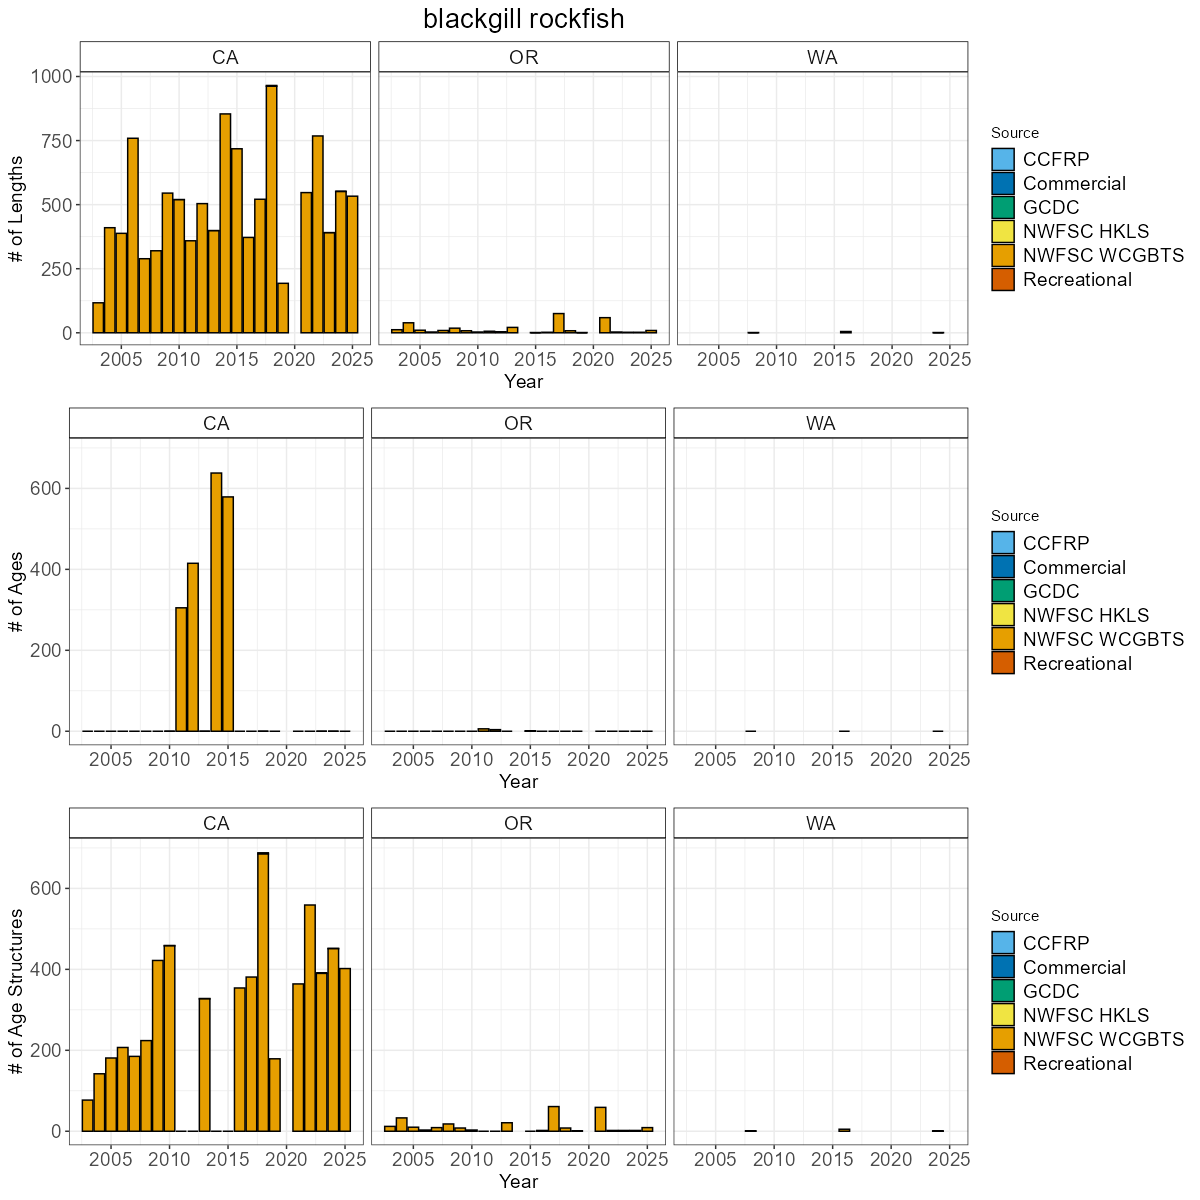
\includegraphics[width=0.95\linewidth,height=\textheight,keepaspectratio]{../plots/state_comparisons/blackgill_rockfish_state_compositions.png}

}

\caption{Total number of available lengths, read ages, and unread age
structures by data source by year for blackgill rockfish. Note the
y-axis maximum may differ by data type.}

\end{figure}%

\begin{figure}[H]

{\centering 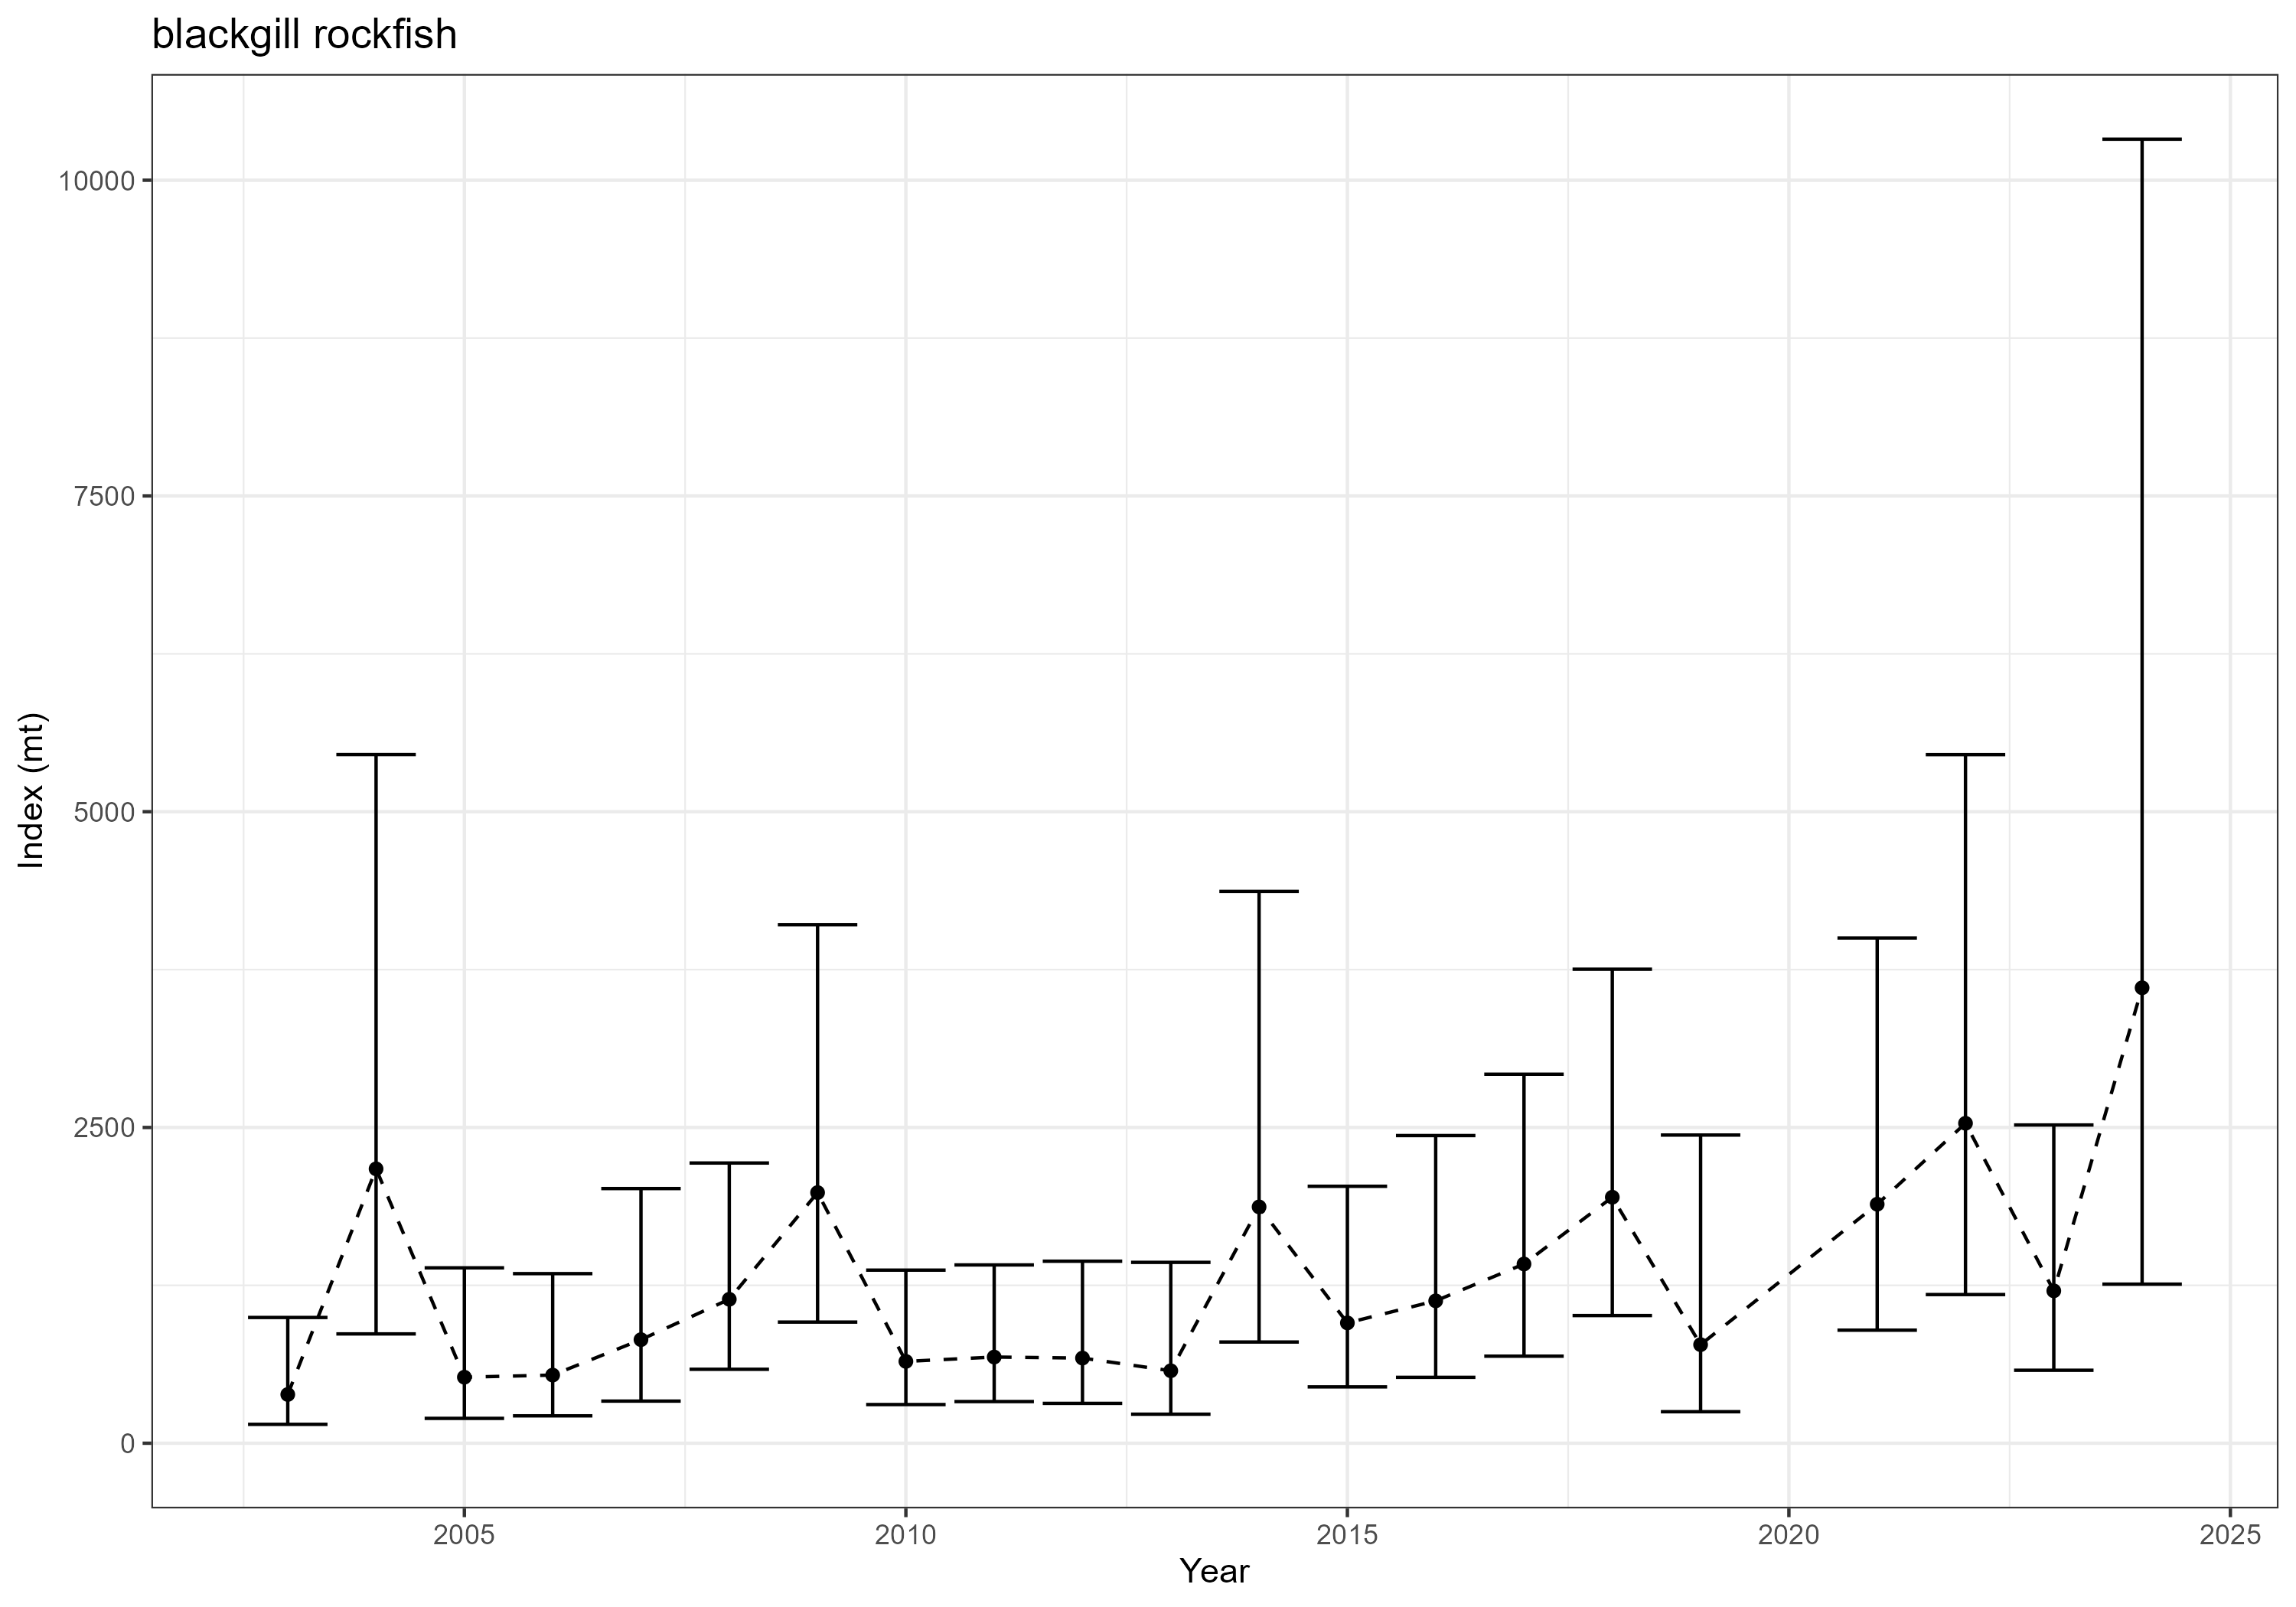
\includegraphics[width=0.95\linewidth,height=\textheight,keepaspectratio]{../plots/wcgbts_indices/blackgill_rockfish_index.png}

}

\caption{Estimated relative index of abundance for blackgill rockfish
from the NWFSC WCGBTS.}

\end{figure}%

\begin{figure}[H]

{\centering 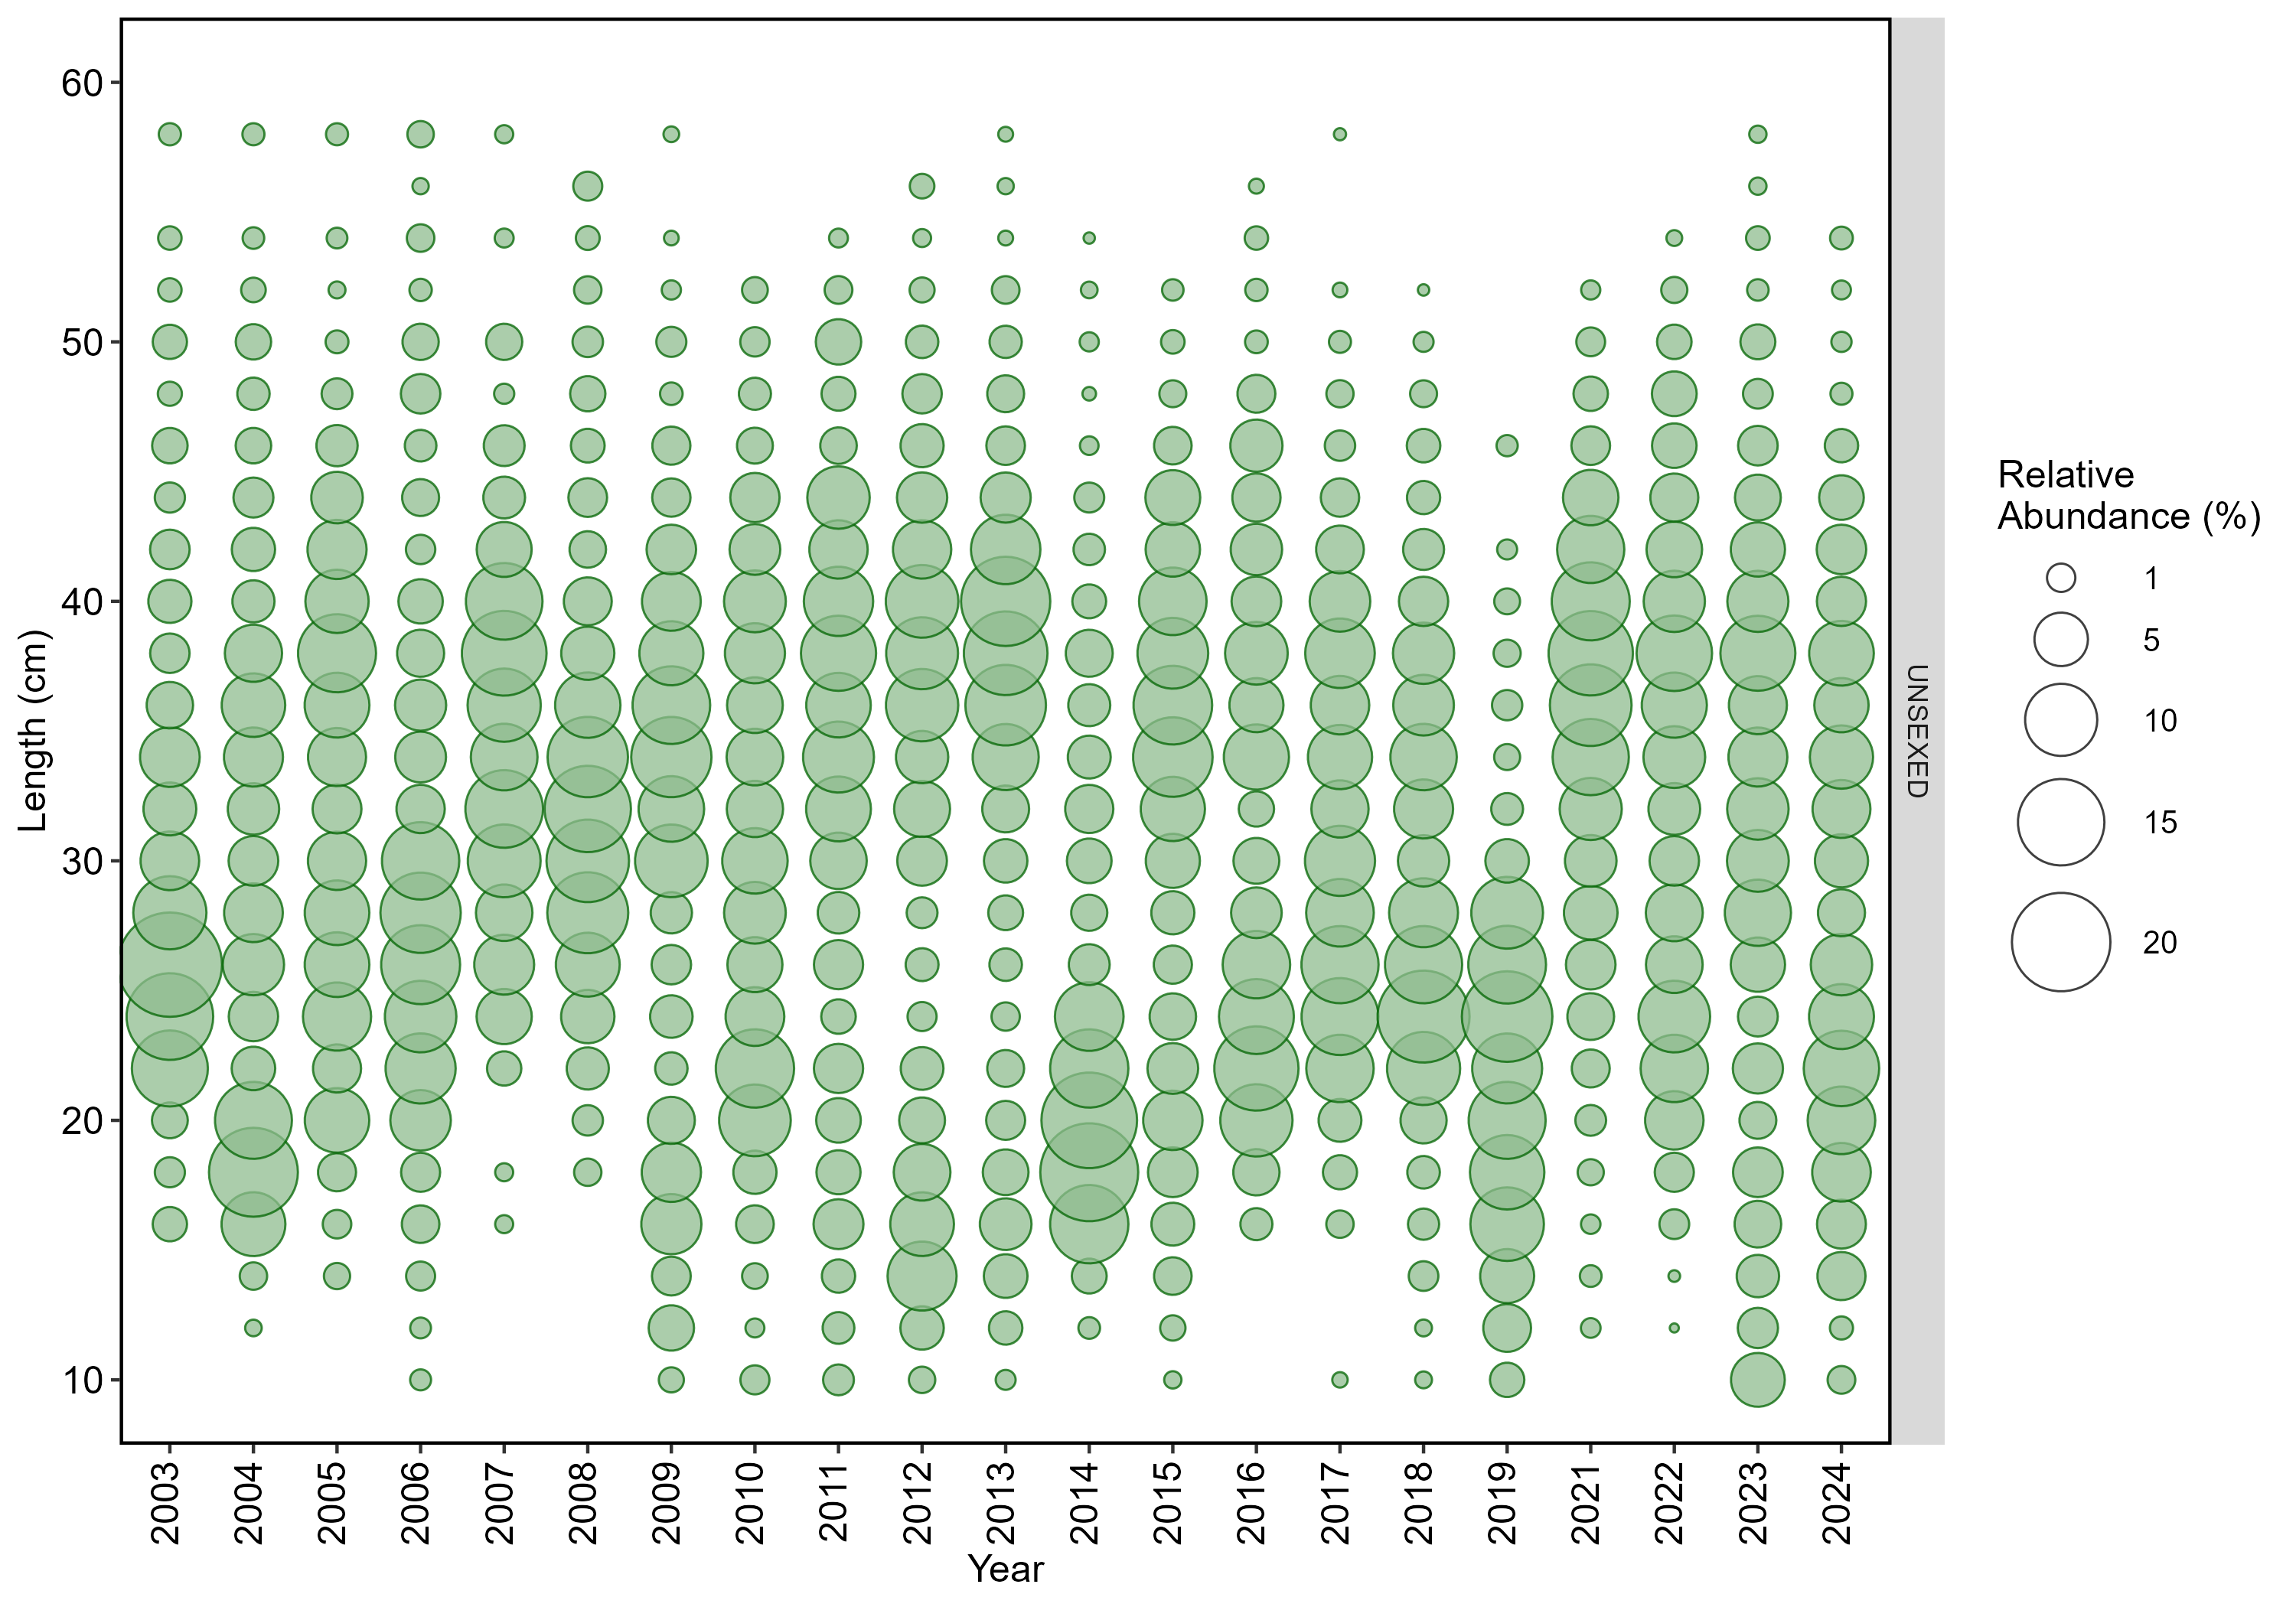
\includegraphics[width=0.95\linewidth,height=\textheight,keepaspectratio]{../plots/wcgbts_comps/plots/blackgill rockfish_length_frequency_sex_0.png}

}

\caption{Length (cm) compostion data from the NWFSC WCGBTS for blackgill
rockfish. Size of the circles within a year indicate higher (larger
circles) and lower (smaller circles) proportion observed by length bin.}

\end{figure}%

\newpage{}

\subsection{Bocaccio}\label{bocaccio}

The most recent assessment of bocaccio was an update assessment
conducted in 2017. Across available data, bocaccio have been observed
and sampled by both the NWFSC HKLS and WCGBTS. The NWFSC HKLS observed
bocaccio at an average of 120 sets per year. The NWFSC WCGBTS observed
bocaccio on an average of 53 tows per year. For this species, a total of
837 maturity samples have been collected coastwide (regardless of stock
area), with 737 read maturities.

\begingroup\fontsize{10}{12}\selectfont
\begingroup\fontsize{10}{12}\selectfont

\begin{longtable}[t]{>{\raggedleft\arraybackslash}p{2cm}>{\raggedleft\arraybackslash}p{3.5cm}>{\raggedleft\arraybackslash}p{2cm}>{\raggedleft\arraybackslash}p{2cm}>{\raggedleft\arraybackslash}p{2cm}}
\caption{\label{tab:unnamed-chunk-89}Total number of available lengths, read ages, and unread age structures by data source and
state for bocaccio.}\\
\toprule
State & Source & Lengths & Ages & Age Structures\\
\midrule
\endfirsthead
\caption[]{Total number of available lengths, read ages, and unread age structures by data source and
state for bocaccio. (\textit{continued)}}\\
\toprule
State & Source & Lengths & Ages & Age Structures\\
\midrule
\endhead

\endfoot
\bottomrule
\endlastfoot
CA & NWFSC HKLS & 22,667 & 0 & 14,376\\
CA & NWFSC WCGBTS & 11,222 & 2,760 & 4,559\\
OR & NWFSC WCGBTS & 297 & 20 & 183\\
WA & NWFSC WCGBTS & 522 & 74 & 366\\*
\end{longtable}
\endgroup{}
\endgroup{}

\begin{figure}[H]

{\centering 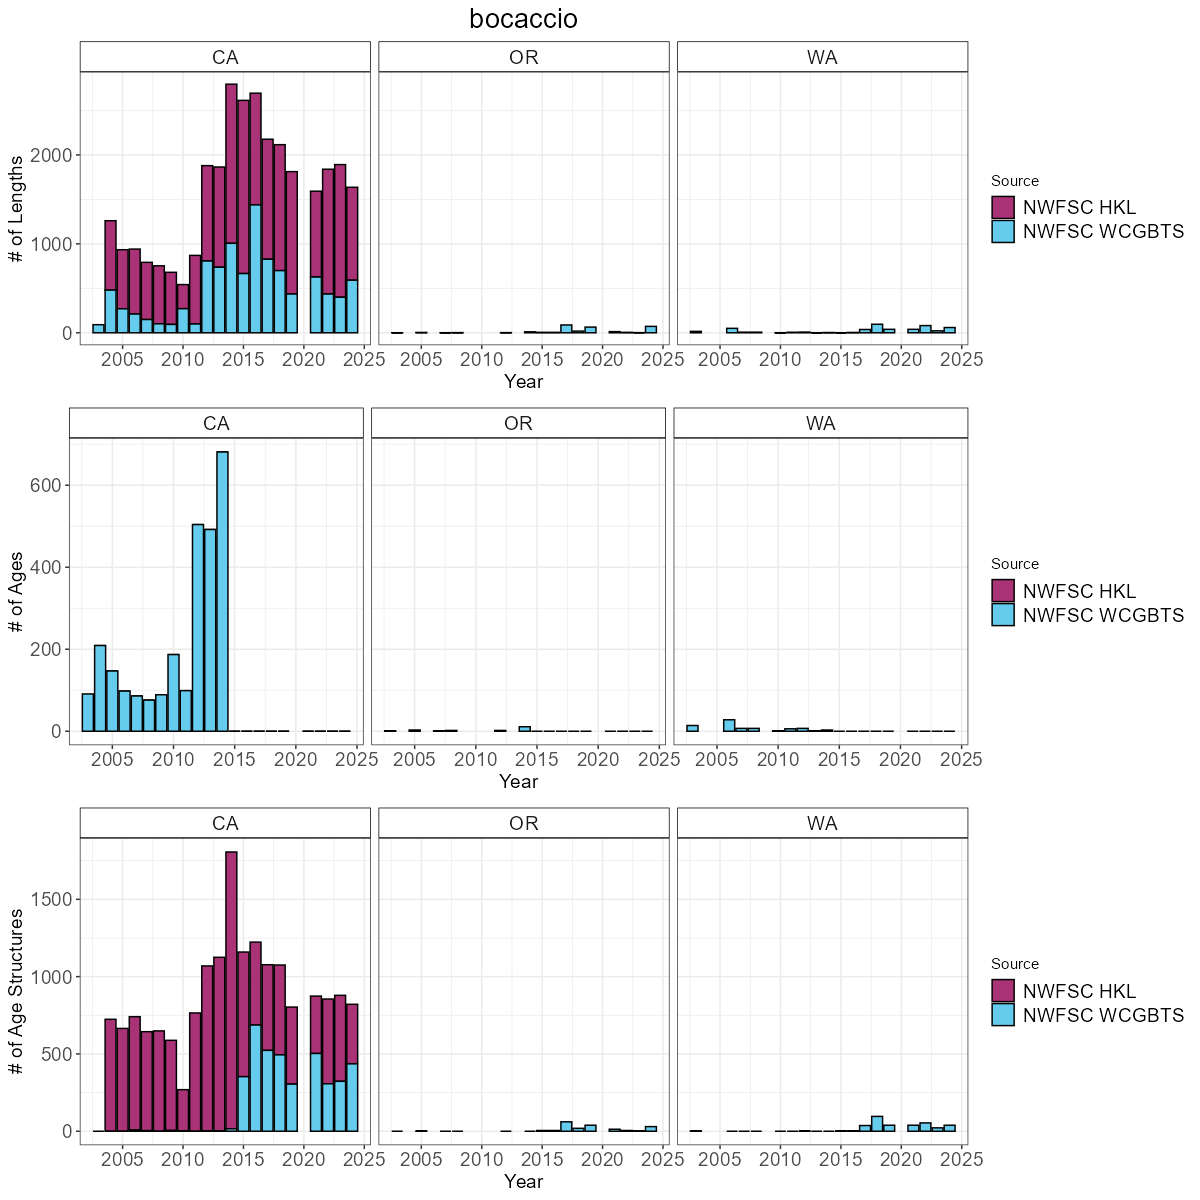
\includegraphics[width=0.95\linewidth,height=\textheight,keepaspectratio]{../plots/state_comparisons/bocaccio_state_compositions.png}

}

\caption{Total number of available lengths, read ages, and unread age
structures by data source by year for bocaccio. Note the y-axis maximum
may differ by data type.}

\end{figure}%

\begin{figure}[H]

{\centering 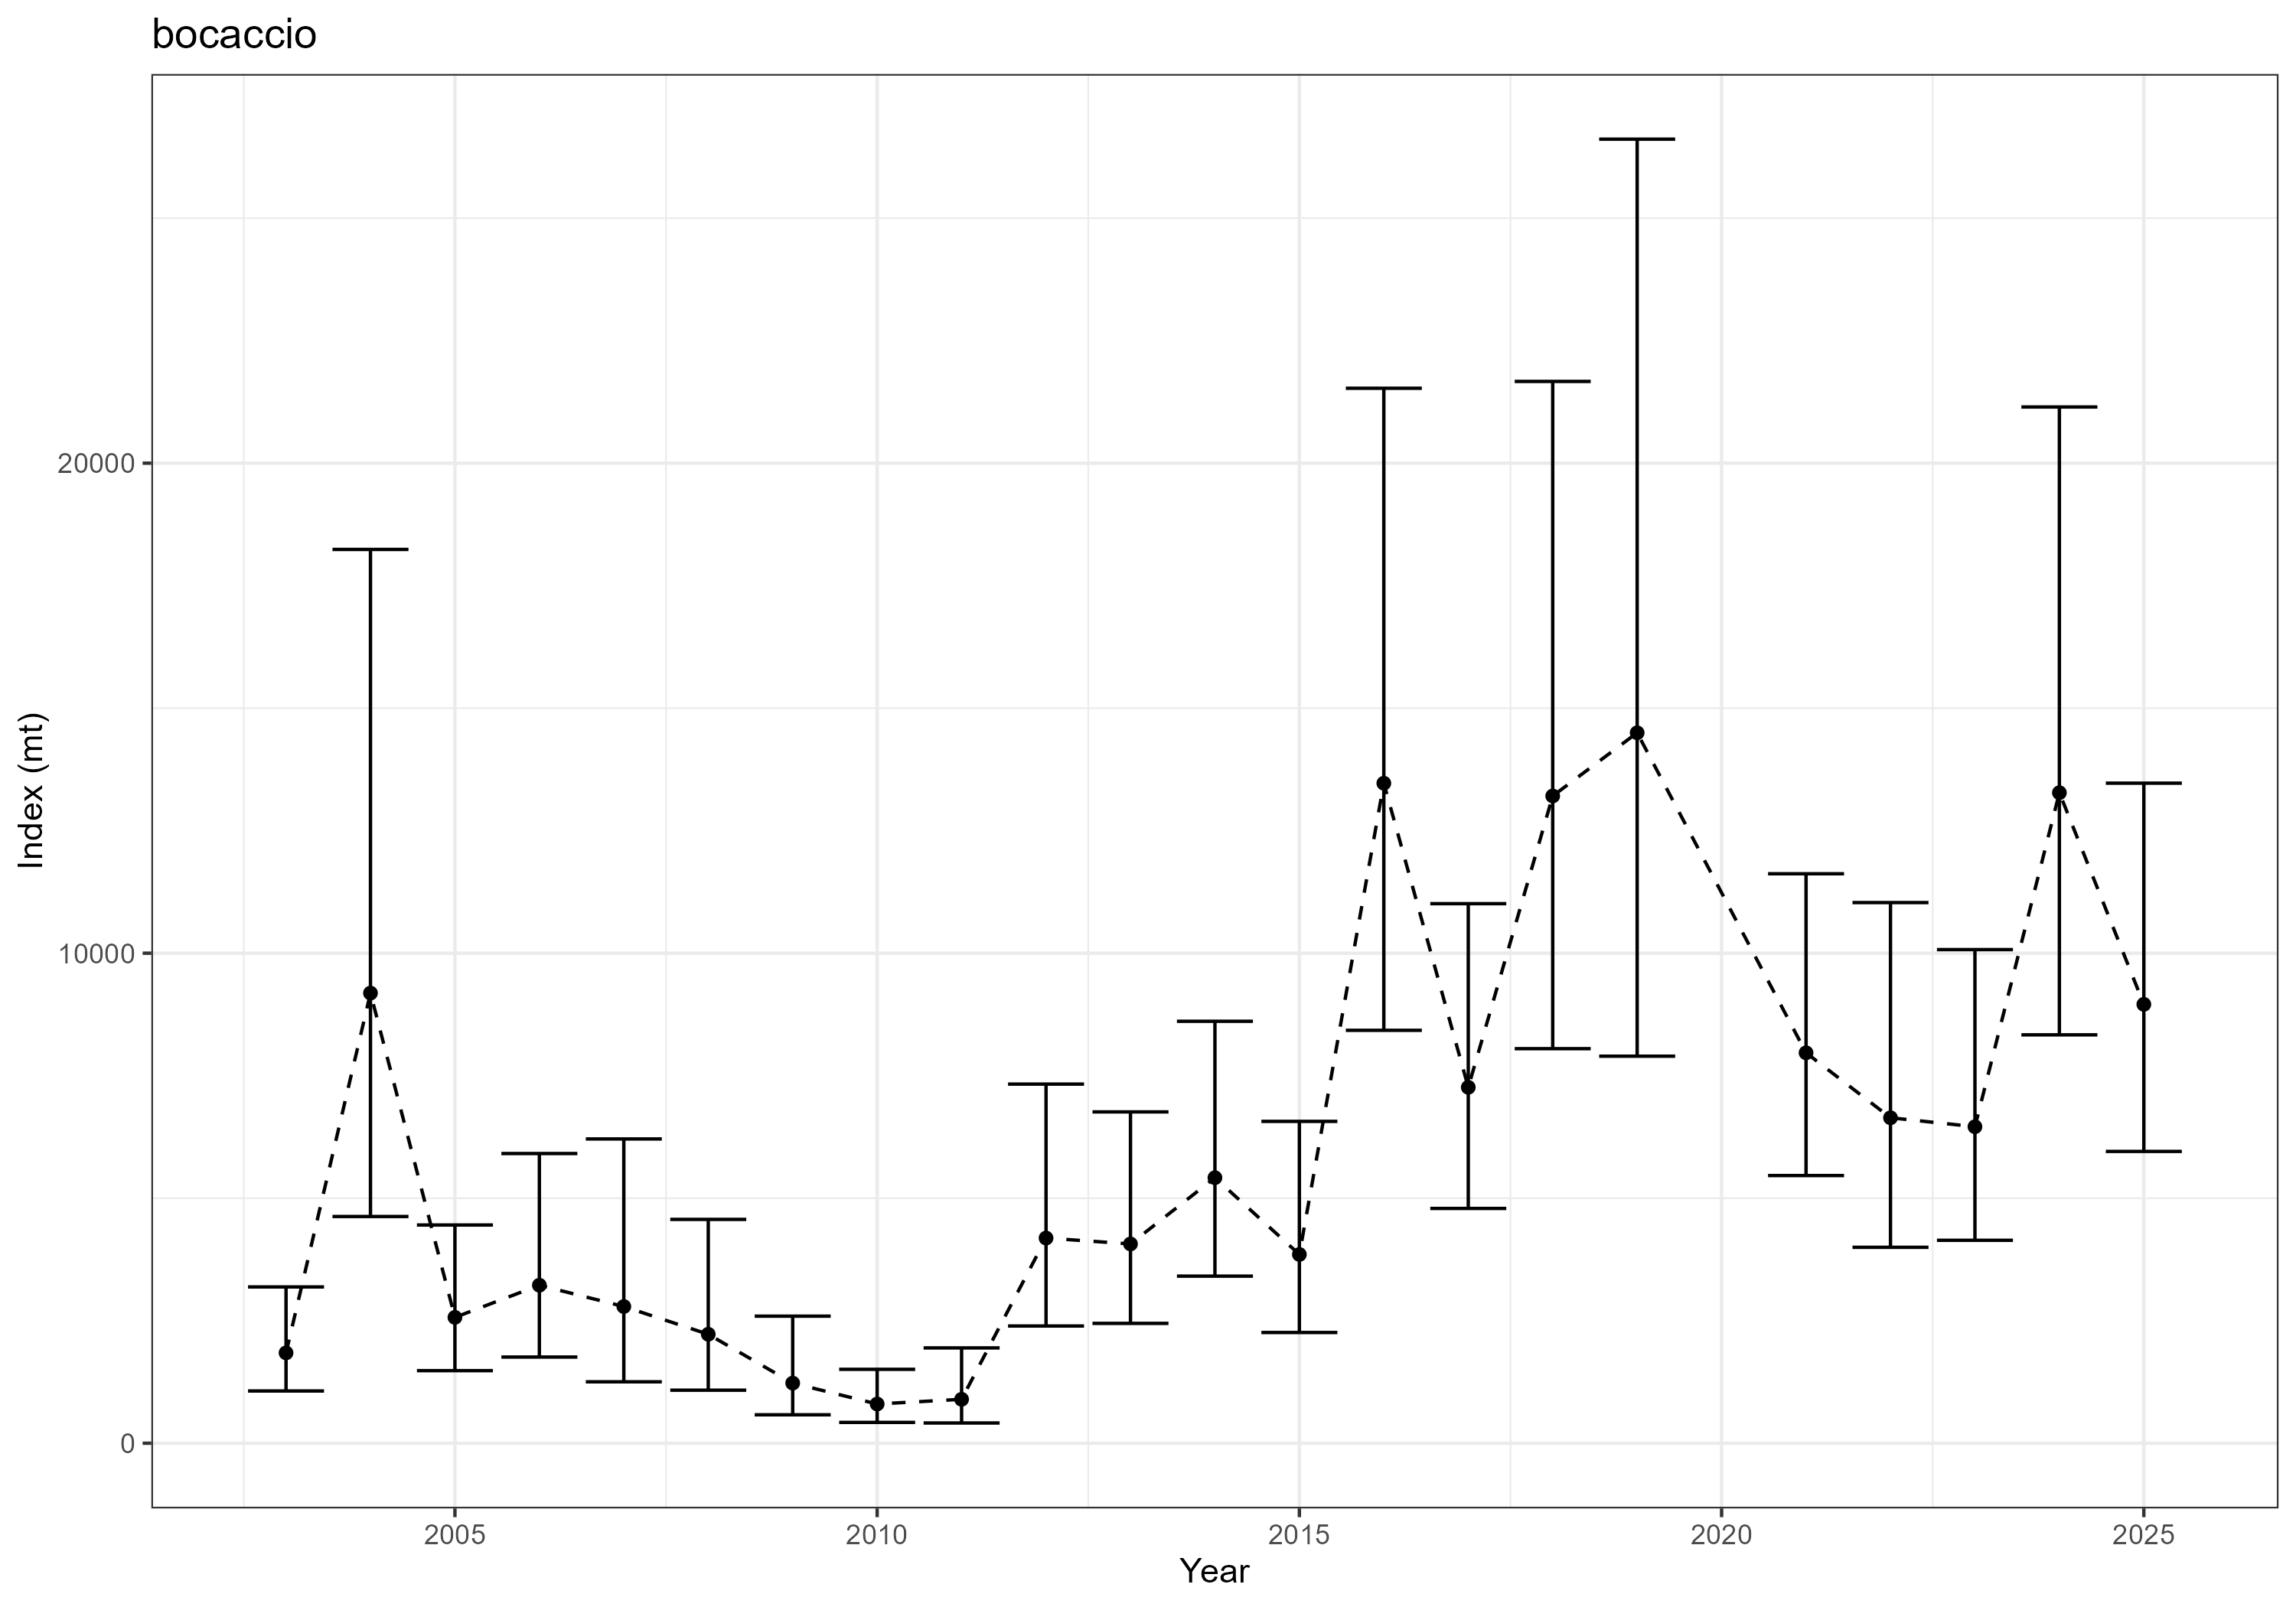
\includegraphics[width=0.95\linewidth,height=\textheight,keepaspectratio]{../plots/wcgbts_indices/bocaccio_index.png}

}

\caption{Estimated relative index of abundance for bocaccio from the
NWFSC WCGBTS.}

\end{figure}%

\begin{figure}[H]

{\centering 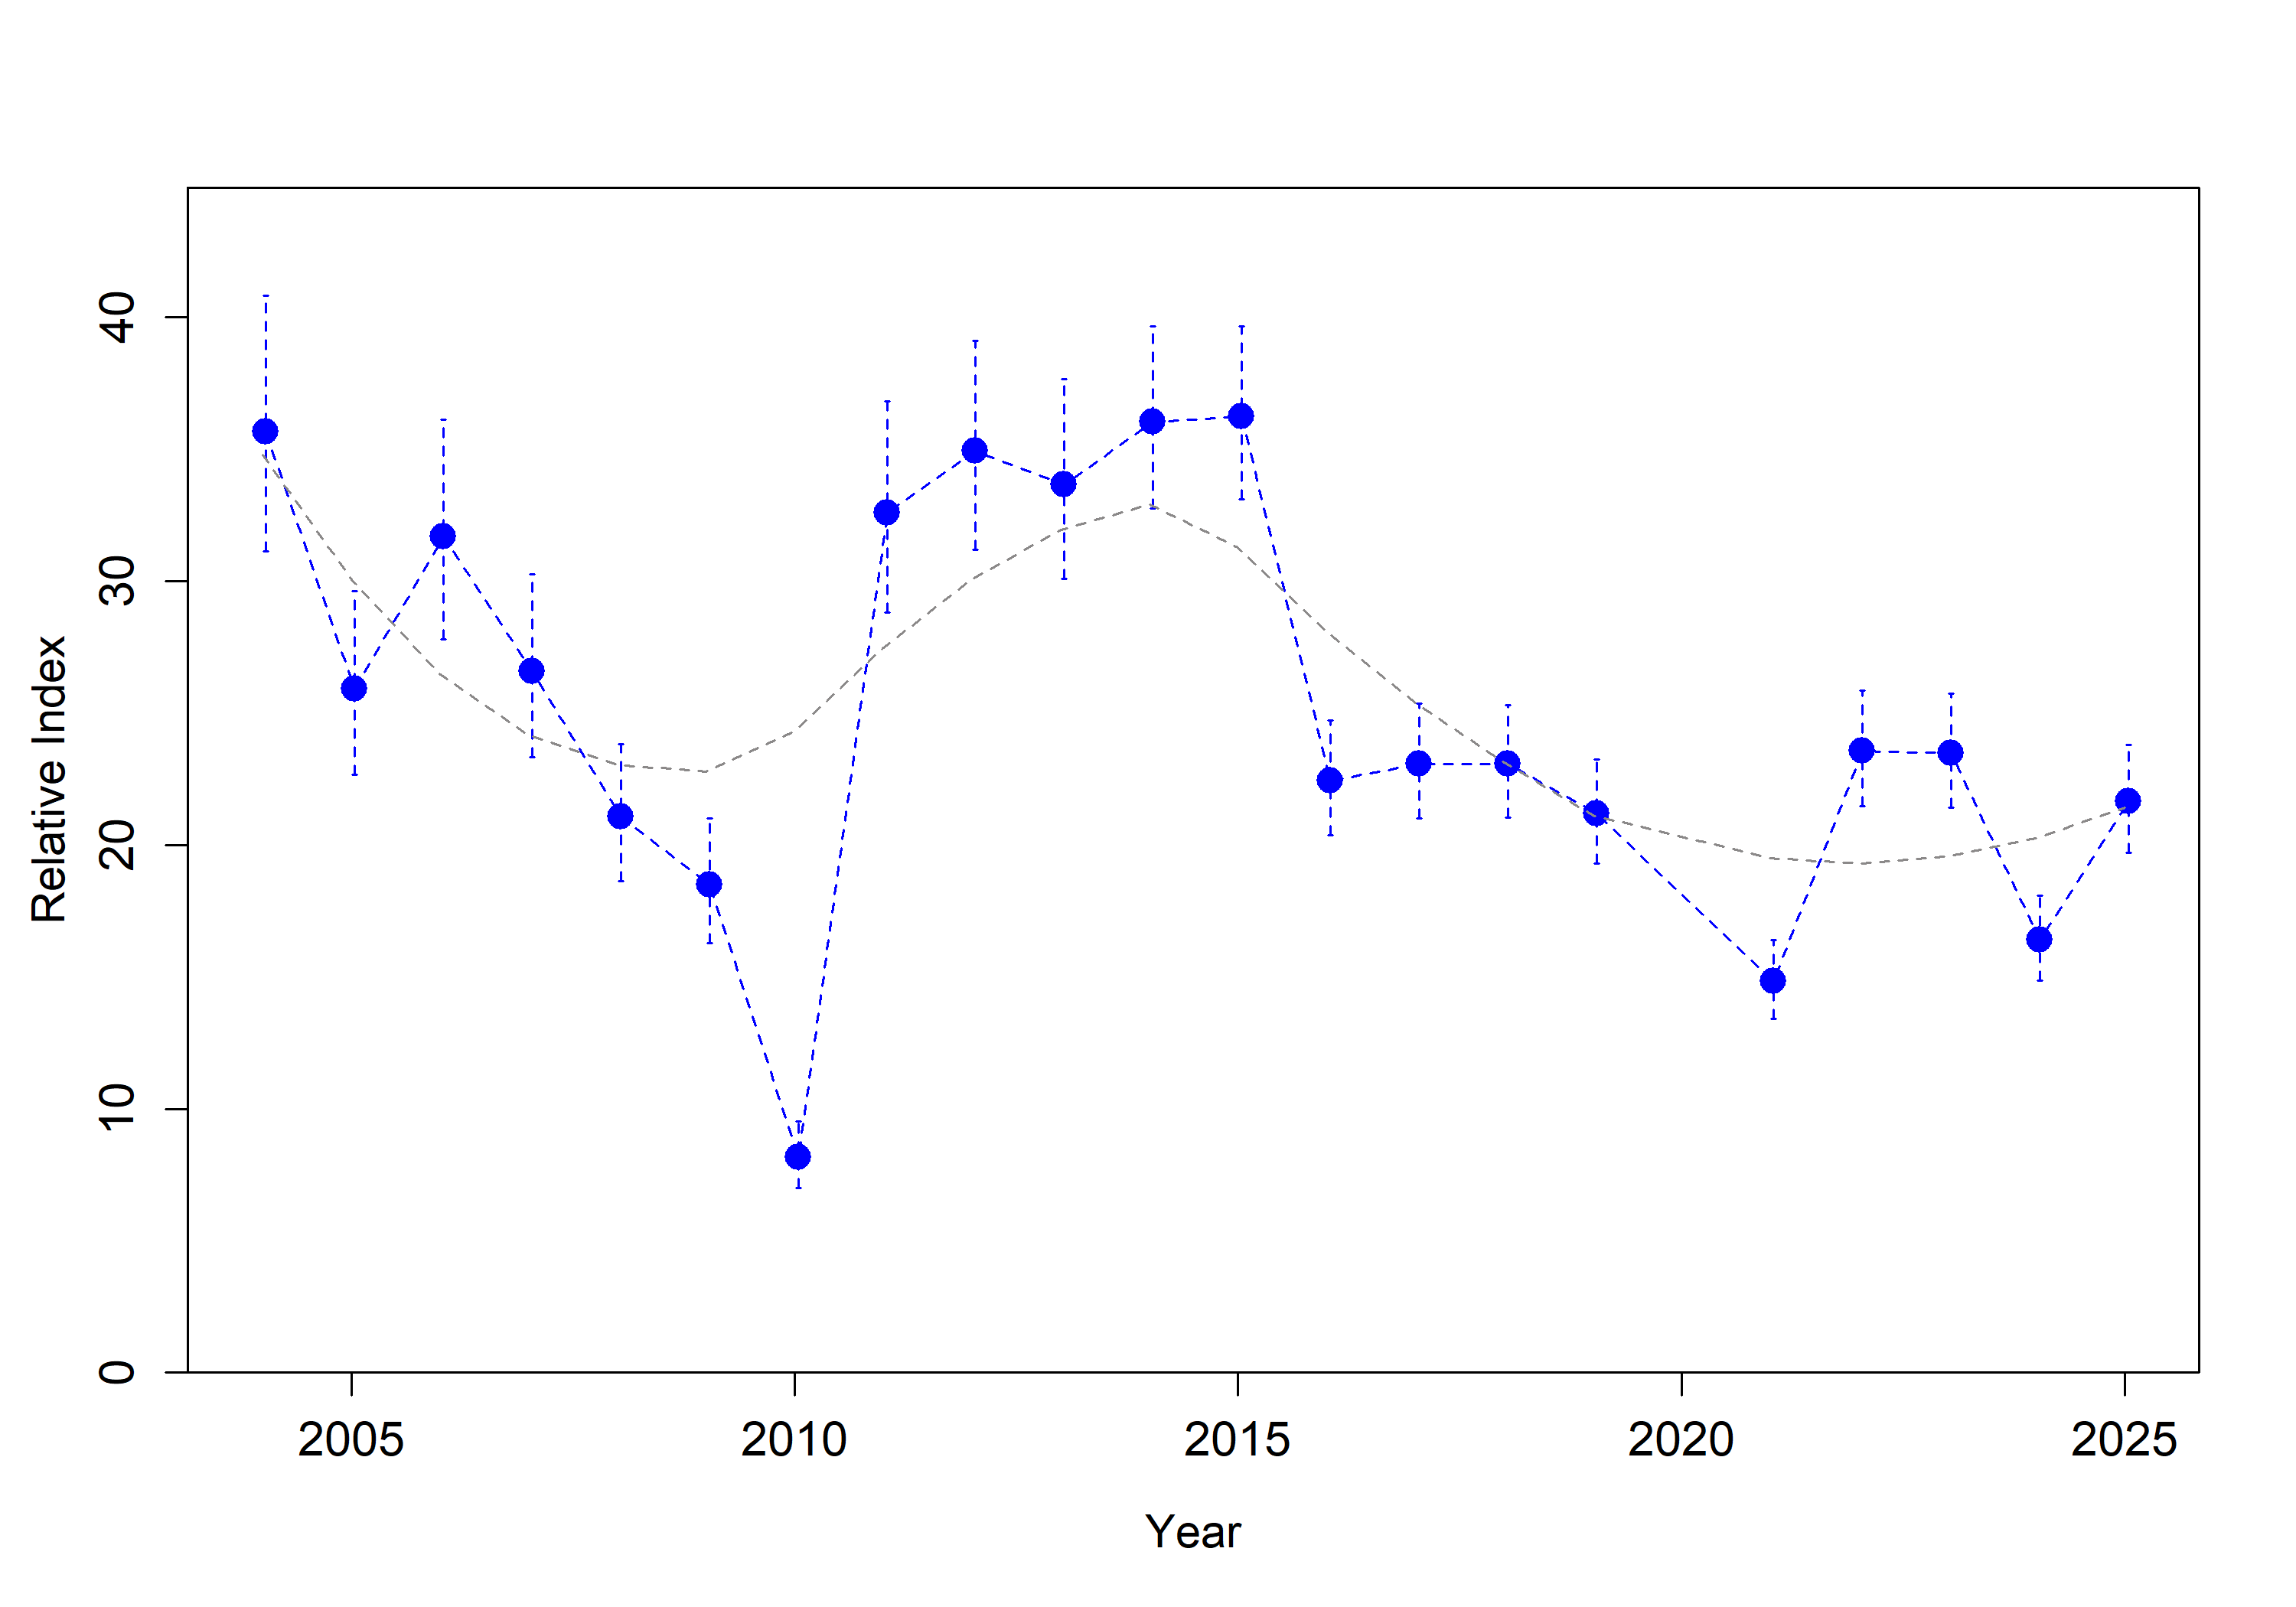
\includegraphics[width=0.95\linewidth,height=\textheight,keepaspectratio]{../plots/hkl_indices/bocaccio_negbinom index.png}

}

\caption{Estimated relative index of abundance for bocaccio from the
NWFSC HKLS.}

\end{figure}%

\begin{figure}[H]

{\centering 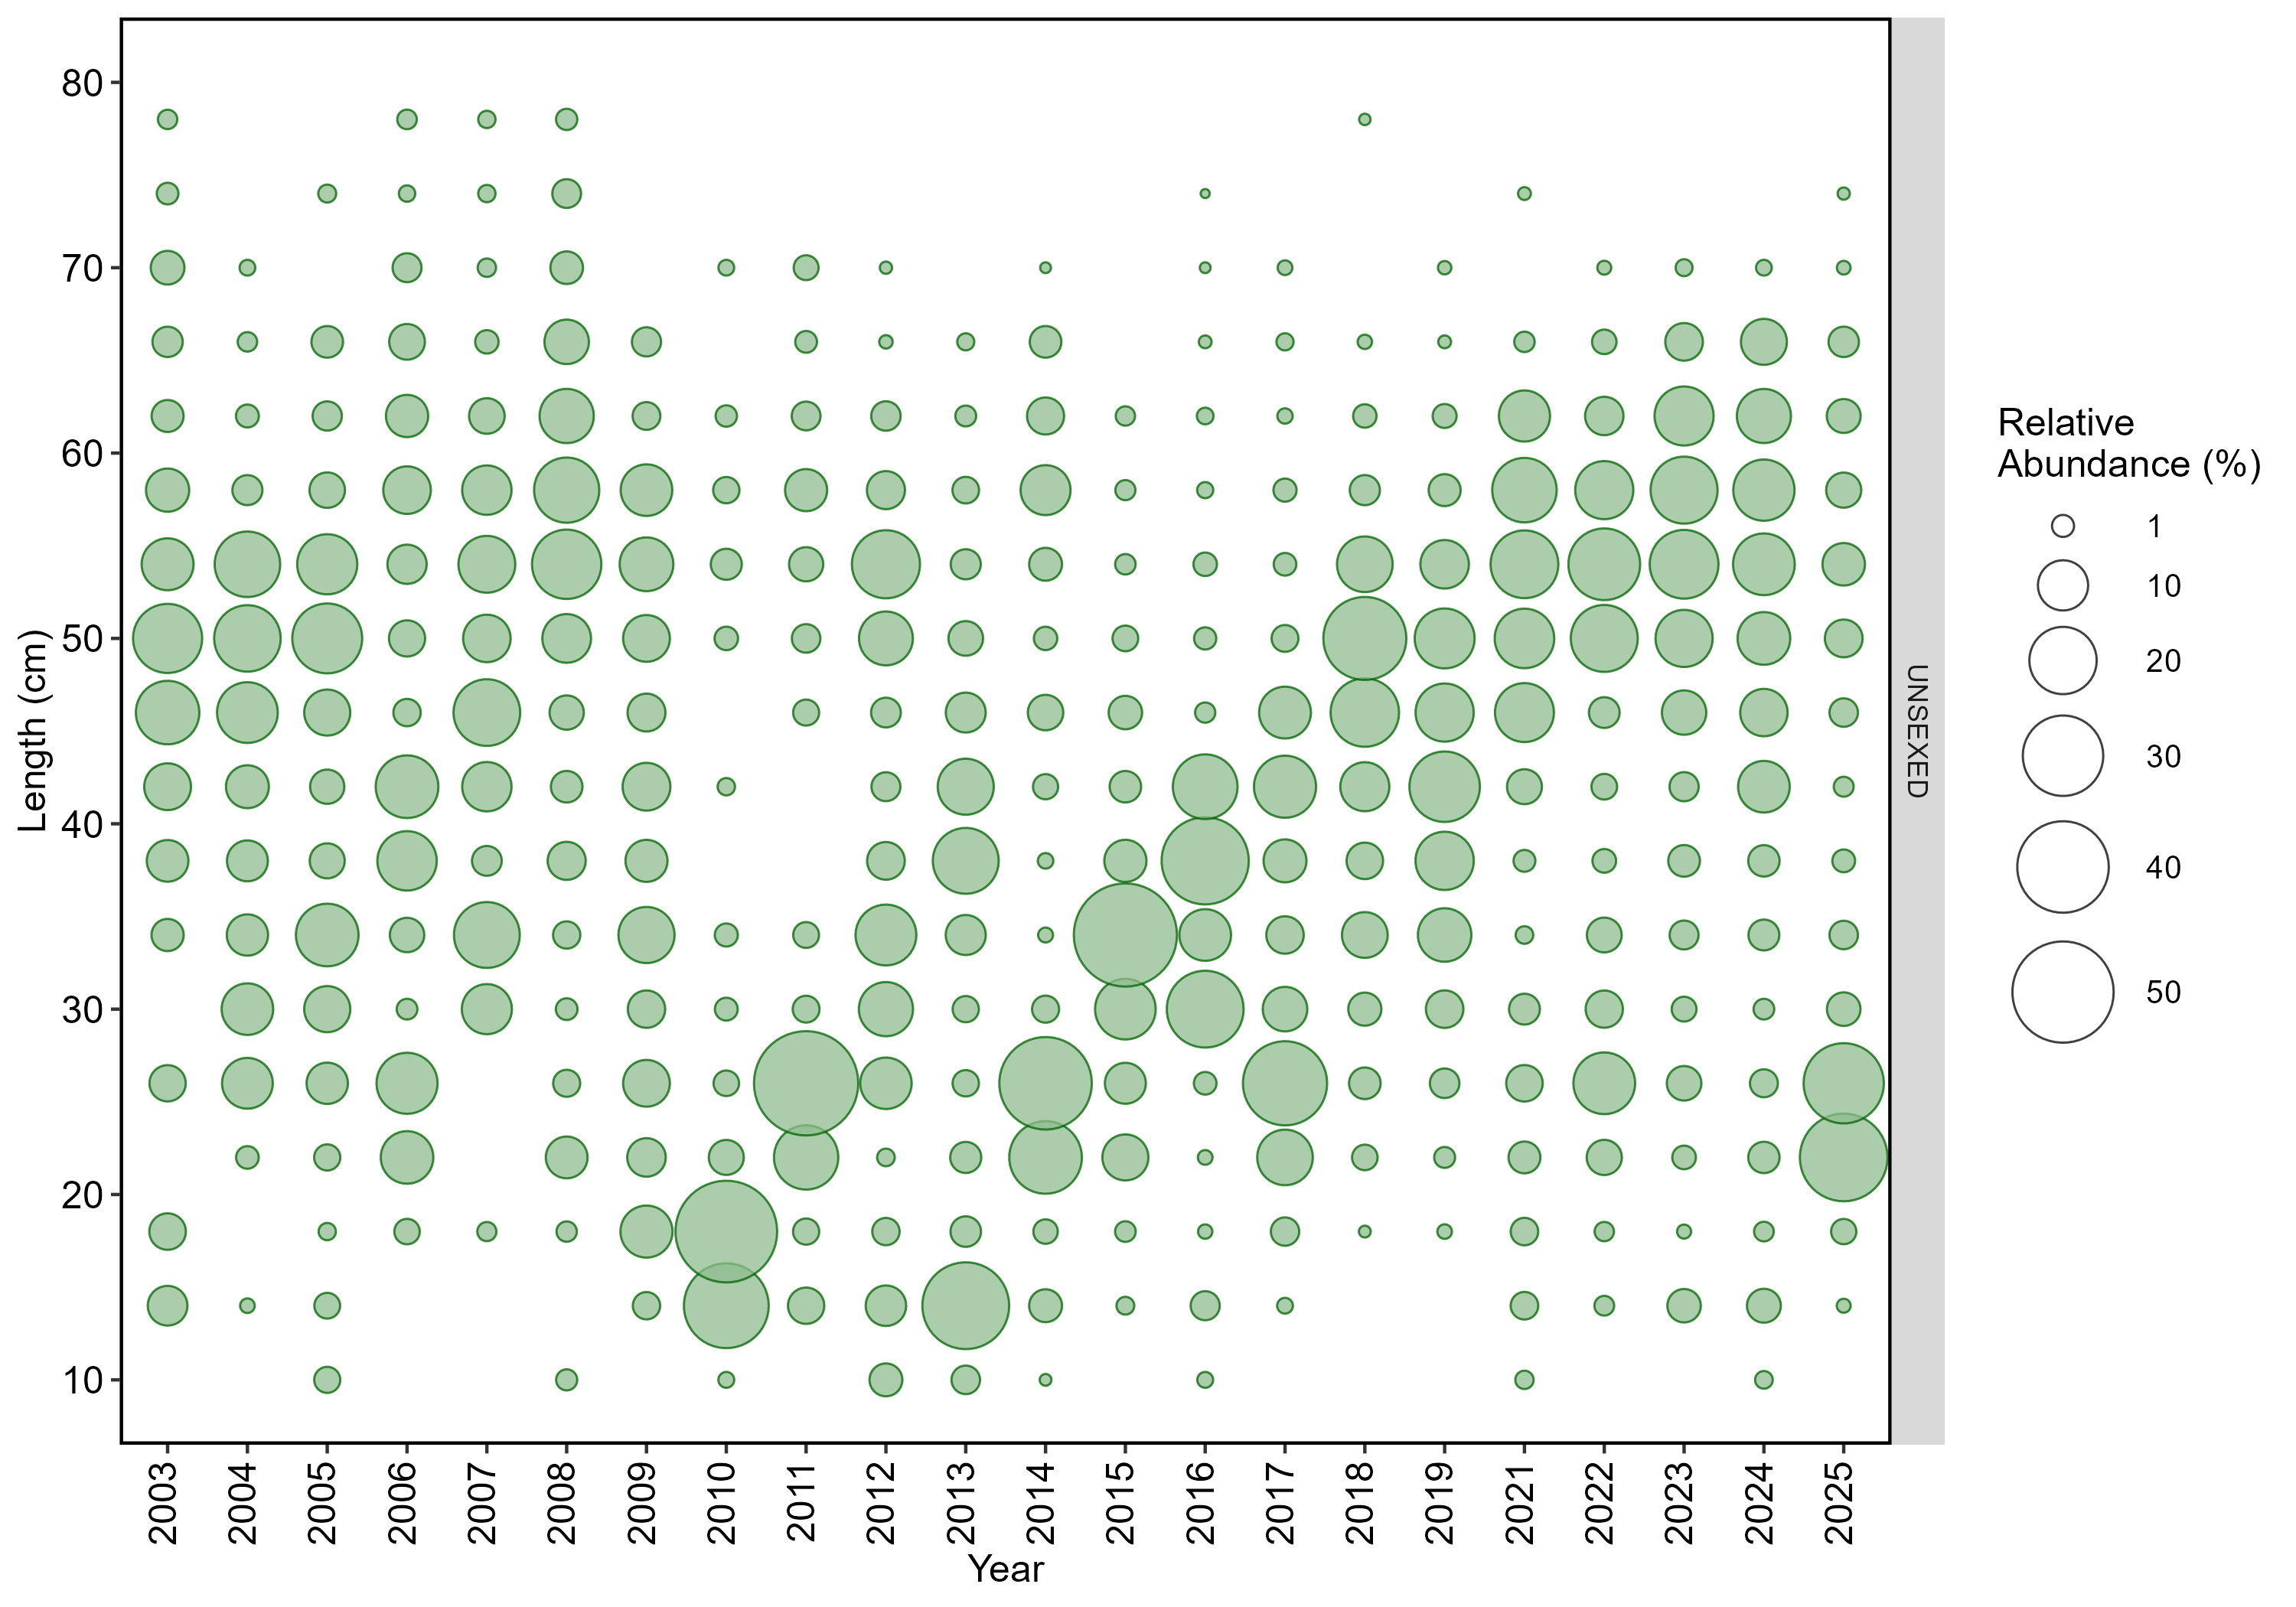
\includegraphics[width=0.95\linewidth,height=\textheight,keepaspectratio]{../plots/wcgbts_comps/plots/bocaccio_length_frequency_sex_0.png}

}

\caption{Length (cm) compostion data from the NWFSC WCGBTS for bocaccio.
Size of the circles within a year indicate higher (larger circles) and
lower (smaller circles) proportion observed by length bin.}

\end{figure}%

\begin{figure}[H]

{\centering 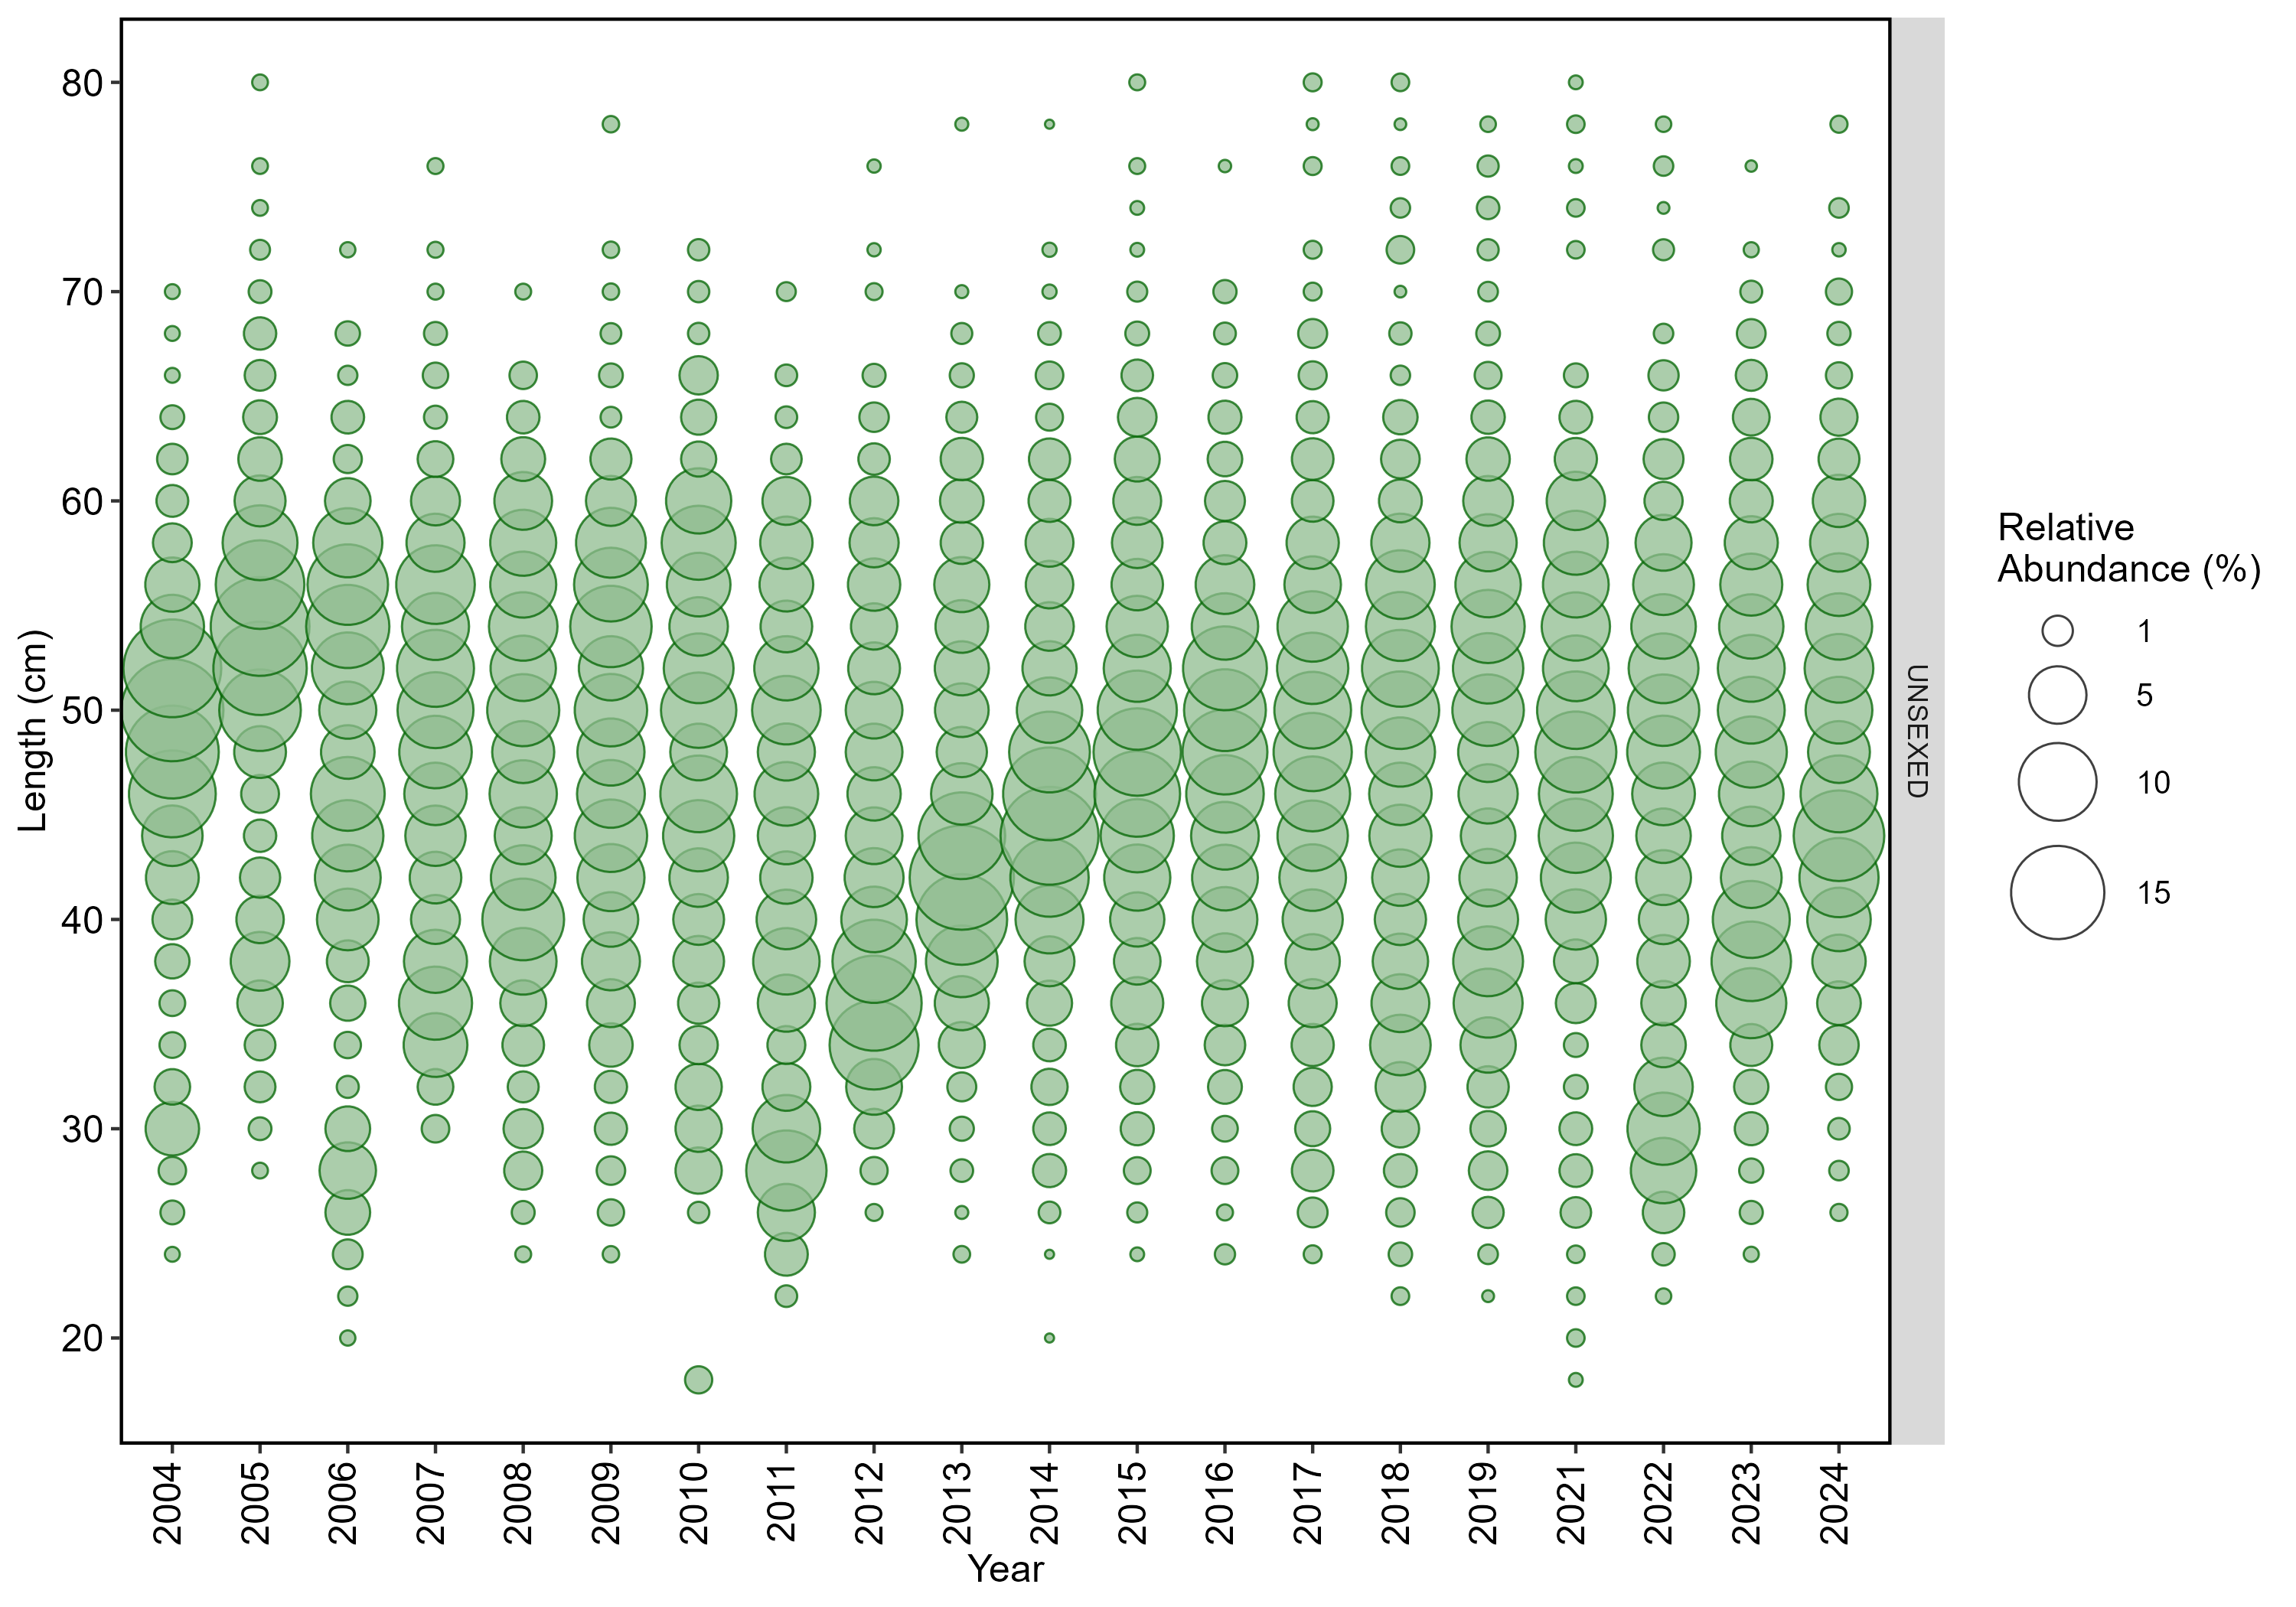
\includegraphics[width=0.95\linewidth,height=\textheight,keepaspectratio]{../plots/hkl_comps/plots/bocaccio_nwfsc_hkl_length_frequency_sex_0.png}

}

\caption{Length (cm) compostion data from the NWFSC HKLS for bocaccio.
Size of the circles within a year indicate higher (larger circles) and
lower (smaller circles) proportion observed by length bin.}

\end{figure}%

\newpage{}

\subsection{California scorpionfish}\label{california-scorpionfish}

The most recent assessment of California scorpionfish was a benchmark
assessment conducted in 2017. Across available data, California
scorpionfish have been observed and sampled by both the NWFSC HKLS and
WCGBTS. The NWFSC HKLS observed California scorpionfish at an average of
2 sets per year. The NWFSC WCGBTS observed California scorpionfish on an
average of 13 tows per year. For this species, a total of 0 maturity
samples have been collected coastwide (regardless of stock area).

\begingroup\fontsize{10}{12}\selectfont
\begingroup\fontsize{10}{12}\selectfont

\begin{longtable}[t]{>{\raggedleft\arraybackslash}p{2cm}>{\raggedleft\arraybackslash}p{3.5cm}>{\raggedleft\arraybackslash}p{2cm}>{\raggedleft\arraybackslash}p{2cm}>{\raggedleft\arraybackslash}p{2cm}}
\caption{\label{tab:unnamed-chunk-107}Total number of available lengths, read ages, and unread age structures by data source and
state for California scorpionfish.}\\
\toprule
State & Source & Lengths & Ages & Age Structures\\
\midrule
\endfirsthead
\caption[]{Total number of available lengths, read ages, and unread age structures by data source and
state for California scorpionfish. (\textit{continued)}}\\
\toprule
State & Source & Lengths & Ages & Age Structures\\
\midrule
\endhead

\endfoot
\bottomrule
\endlastfoot
CA & NWFSC HKLS & 45 & 0 & 25\\
CA & NWFSC WCGBTS & 4,360 & 911 & 1,174\\*
\end{longtable}
\endgroup{}
\endgroup{}

\begin{figure}[H]

{\centering 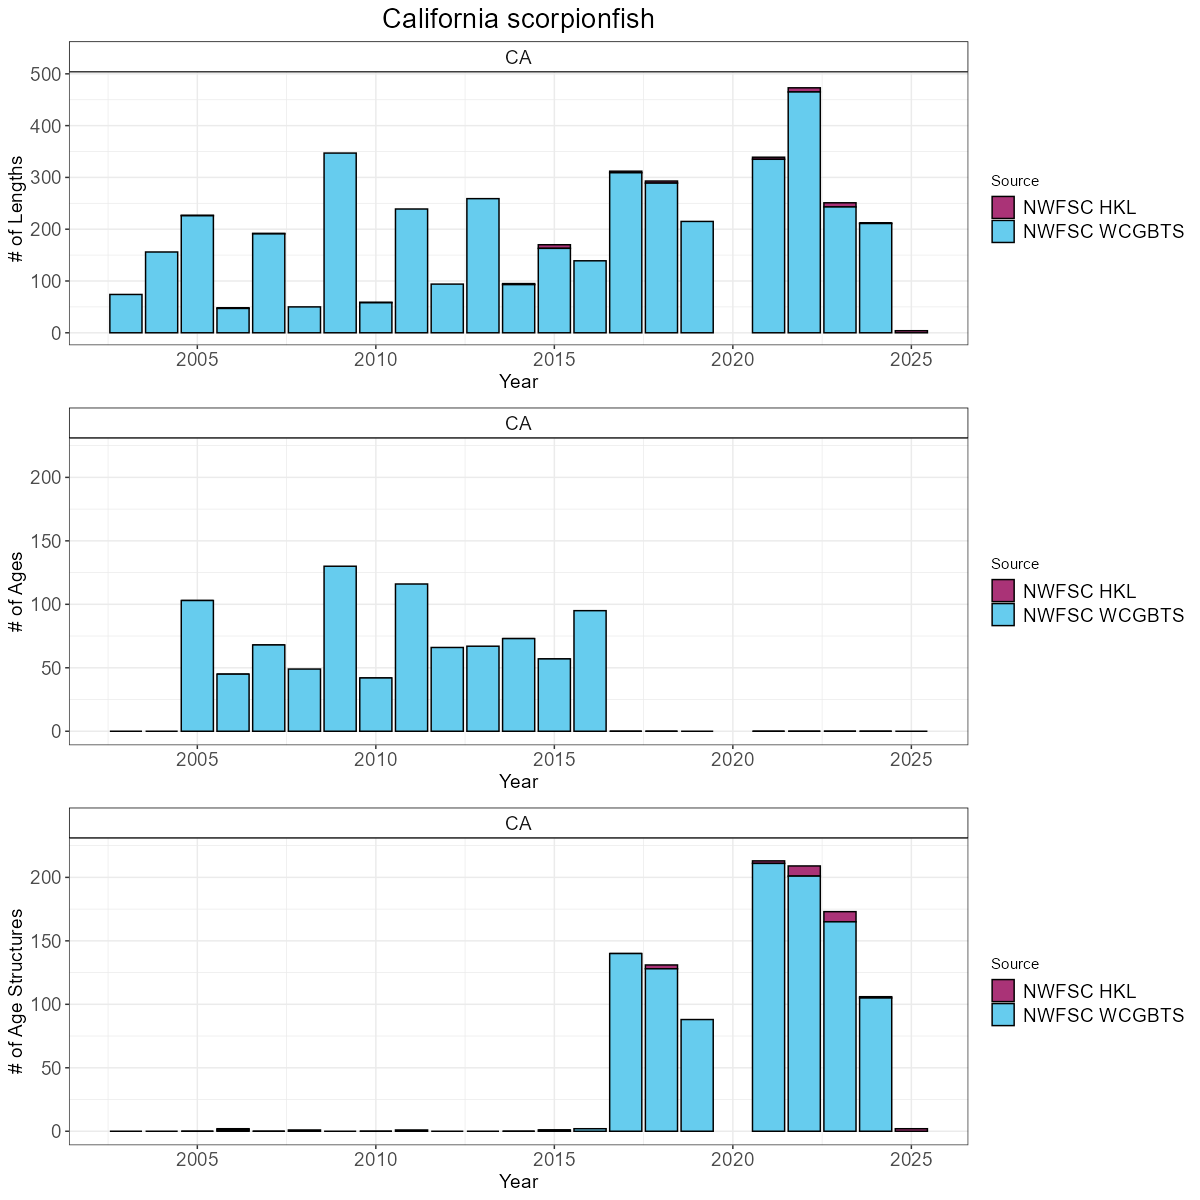
\includegraphics[width=0.95\linewidth,height=\textheight,keepaspectratio]{../plots/state_comparisons/california_scorpionfish_state_compositions.png}

}

\caption{Total number of available lengths, read ages, and unread age
structures by data source by year for California scorpionfish. Note the
y-axis maximum may differ by data type.}

\end{figure}%

\newpage{}

\subsection{Canary rockfish}\label{canary-rockfish}

The most recent assessment of canary rockfish was a benchmark assessment
conducted in 2023. Across available data, canary rockfish have been
observed and sampled by both the NWFSC HKLS and WCGBTS. The NWFSC HKLS
observed canary rockfish at an average of 7 sets per year. The NWFSC
WCGBTS observed canary rockfish on an average of 53 tows per year. For
this species, a total of 1480 maturity samples have been collected
coastwide (regardless of stock area), with 1184 read maturities. ODFW
scientists are planning a research cruise to Cobb Sea Mount in the
summer of 2026 to sample age and sex distributions of this rockfish
species and others.

\begingroup\fontsize{10}{12}\selectfont
\begingroup\fontsize{10}{12}\selectfont

\begin{longtable}[t]{>{\raggedleft\arraybackslash}p{2cm}>{\raggedleft\arraybackslash}p{3.5cm}>{\raggedleft\arraybackslash}p{2cm}>{\raggedleft\arraybackslash}p{2cm}>{\raggedleft\arraybackslash}p{2cm}}
\caption{\label{tab:unnamed-chunk-124}Total number of available lengths, read ages, and unread age structures by data source and
state for canary rockfish.}\\
\toprule
State & Source & Lengths & Ages & Age Structures\\
\midrule
\endfirsthead
\caption[]{Total number of available lengths, read ages, and unread age structures by data source and
state for canary rockfish. (\textit{continued)}}\\
\toprule
State & Source & Lengths & Ages & Age Structures\\
\midrule
\endhead

\endfoot
\bottomrule
\endlastfoot
CA & NWFSC HKLS & 433 & 368 & 60\\
CA & NWFSC WCGBTS & 3,693 & 1,854 & 300\\
OR & NWFSC WCGBTS & 5,103 & 3,189 & 246\\
WA & NWFSC WCGBTS & 6,613 & 3,430 & 521\\*
\end{longtable}
\endgroup{}
\endgroup{}

\begin{figure}[H]

{\centering 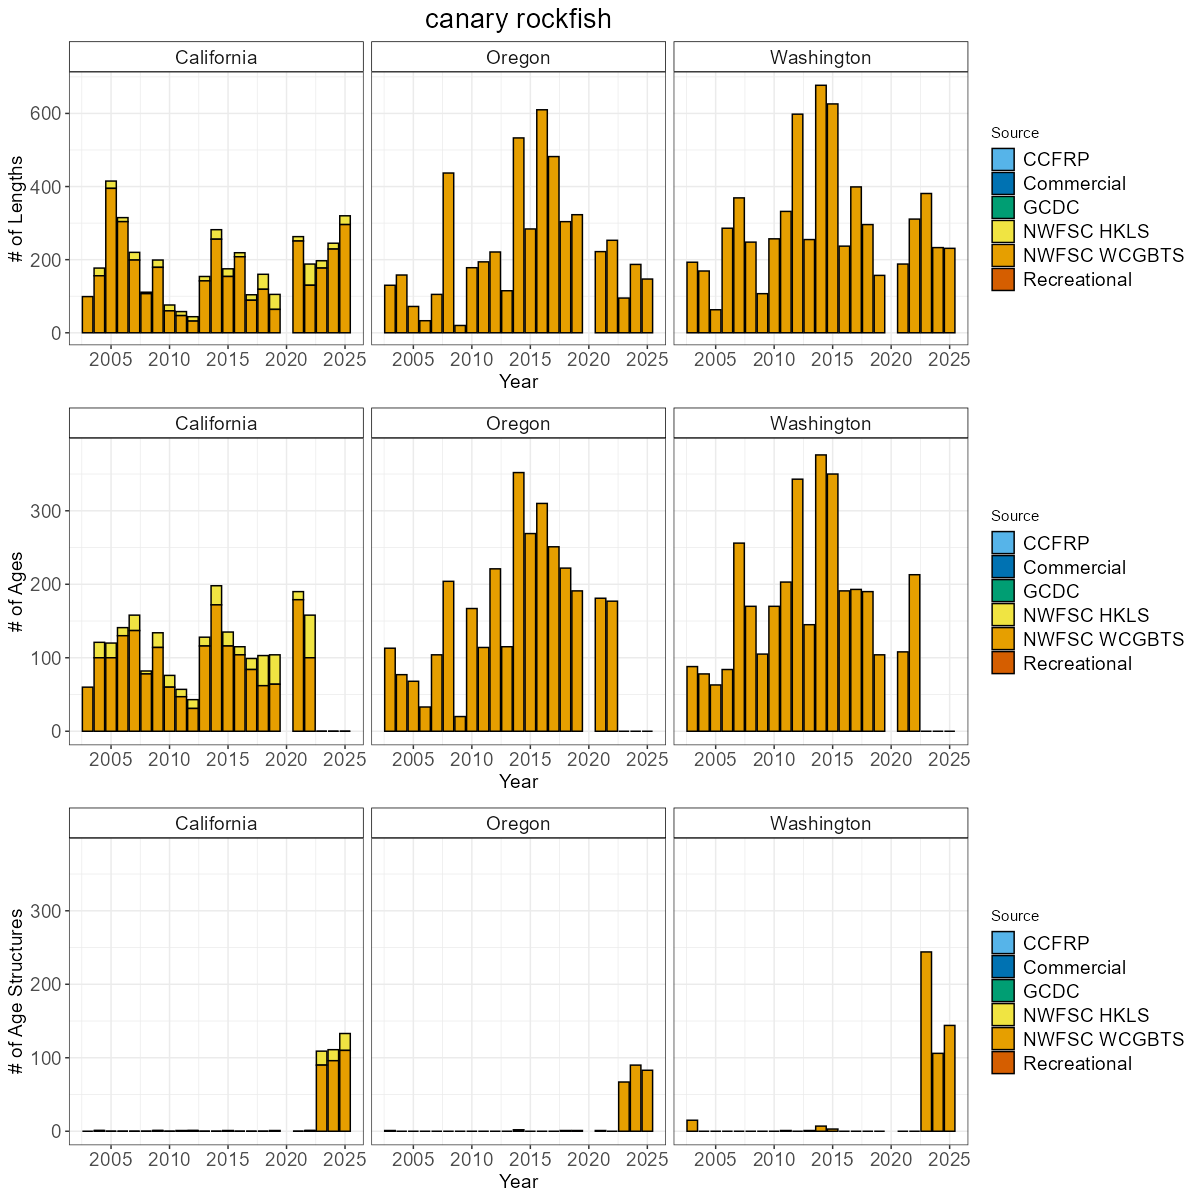
\includegraphics[width=0.95\linewidth,height=\textheight,keepaspectratio]{../plots/state_comparisons/canary_rockfish_state_compositions.png}

}

\caption{Total number of available lengths, read ages, and unread age
structures by data source by year for canary rockfish. Note the y-axis
maximum may differ by data type.}

\end{figure}%

\begin{figure}[H]

{\centering 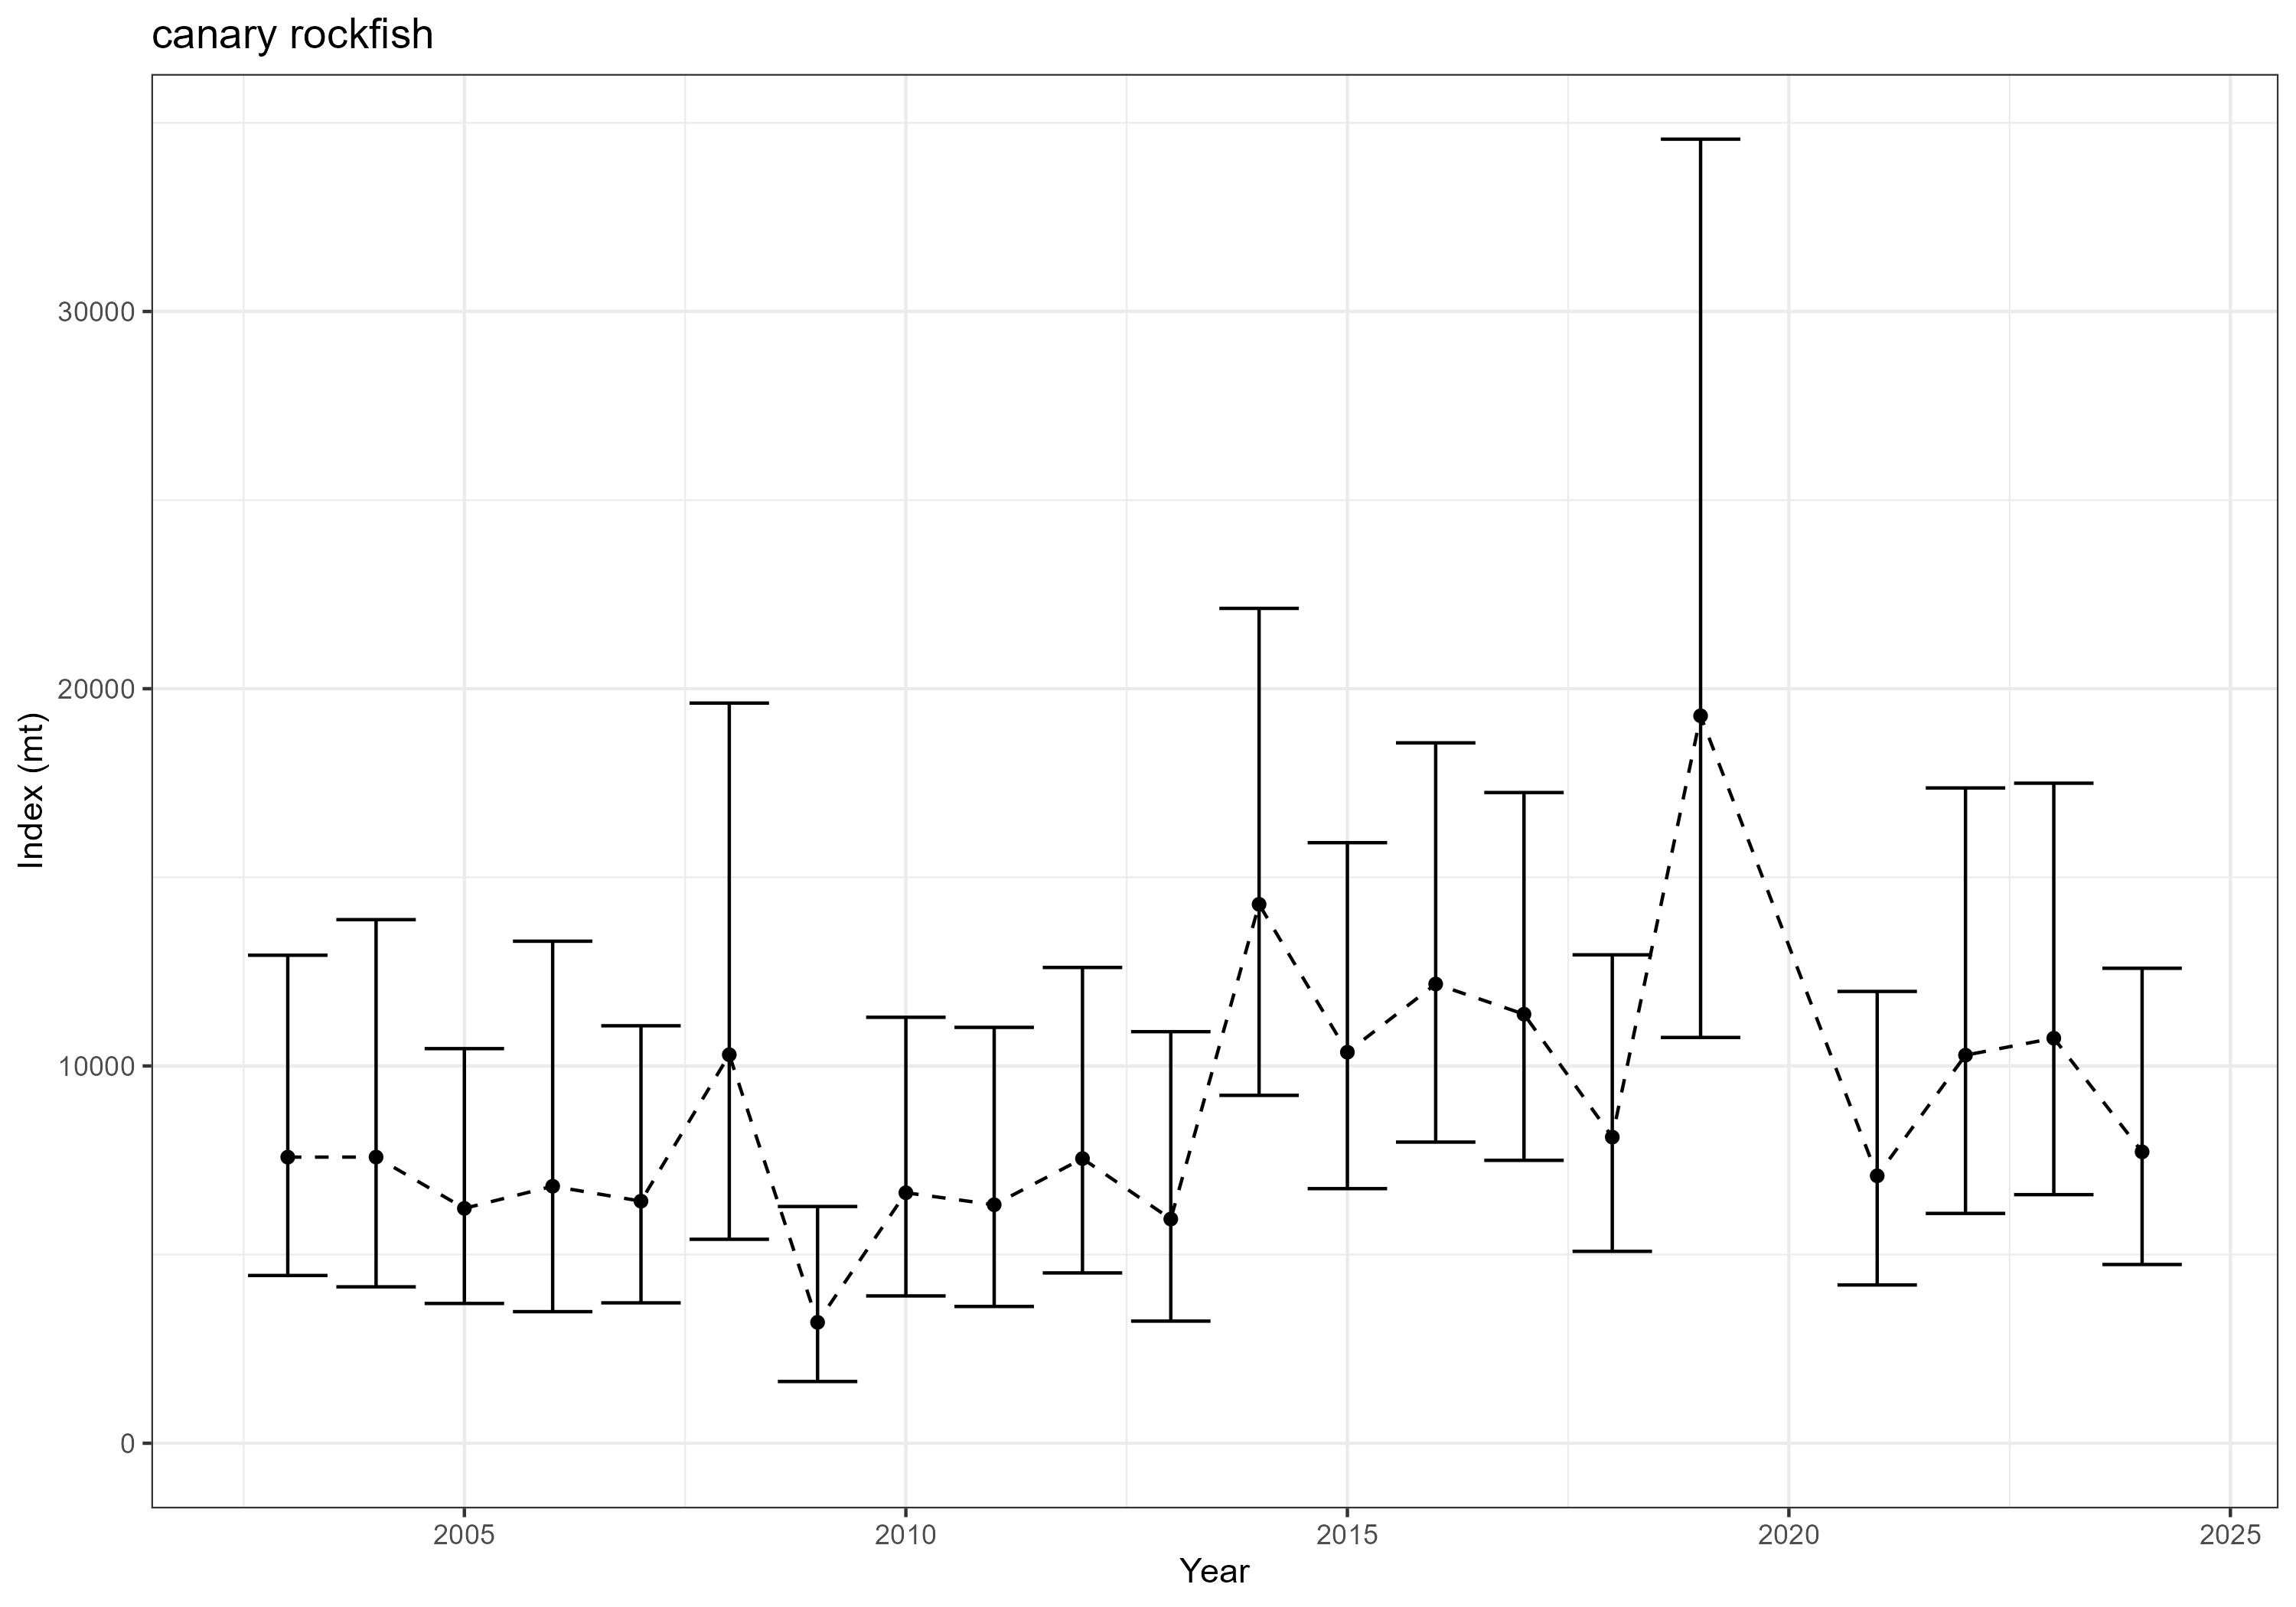
\includegraphics[width=0.95\linewidth,height=\textheight,keepaspectratio]{../plots/wcgbts_indices/canary_rockfish_index.png}

}

\caption{Estimated relative index of abundance for canary rockfish from
the NWFSC WCGBTS.}

\end{figure}%

\begin{figure}[H]

{\centering 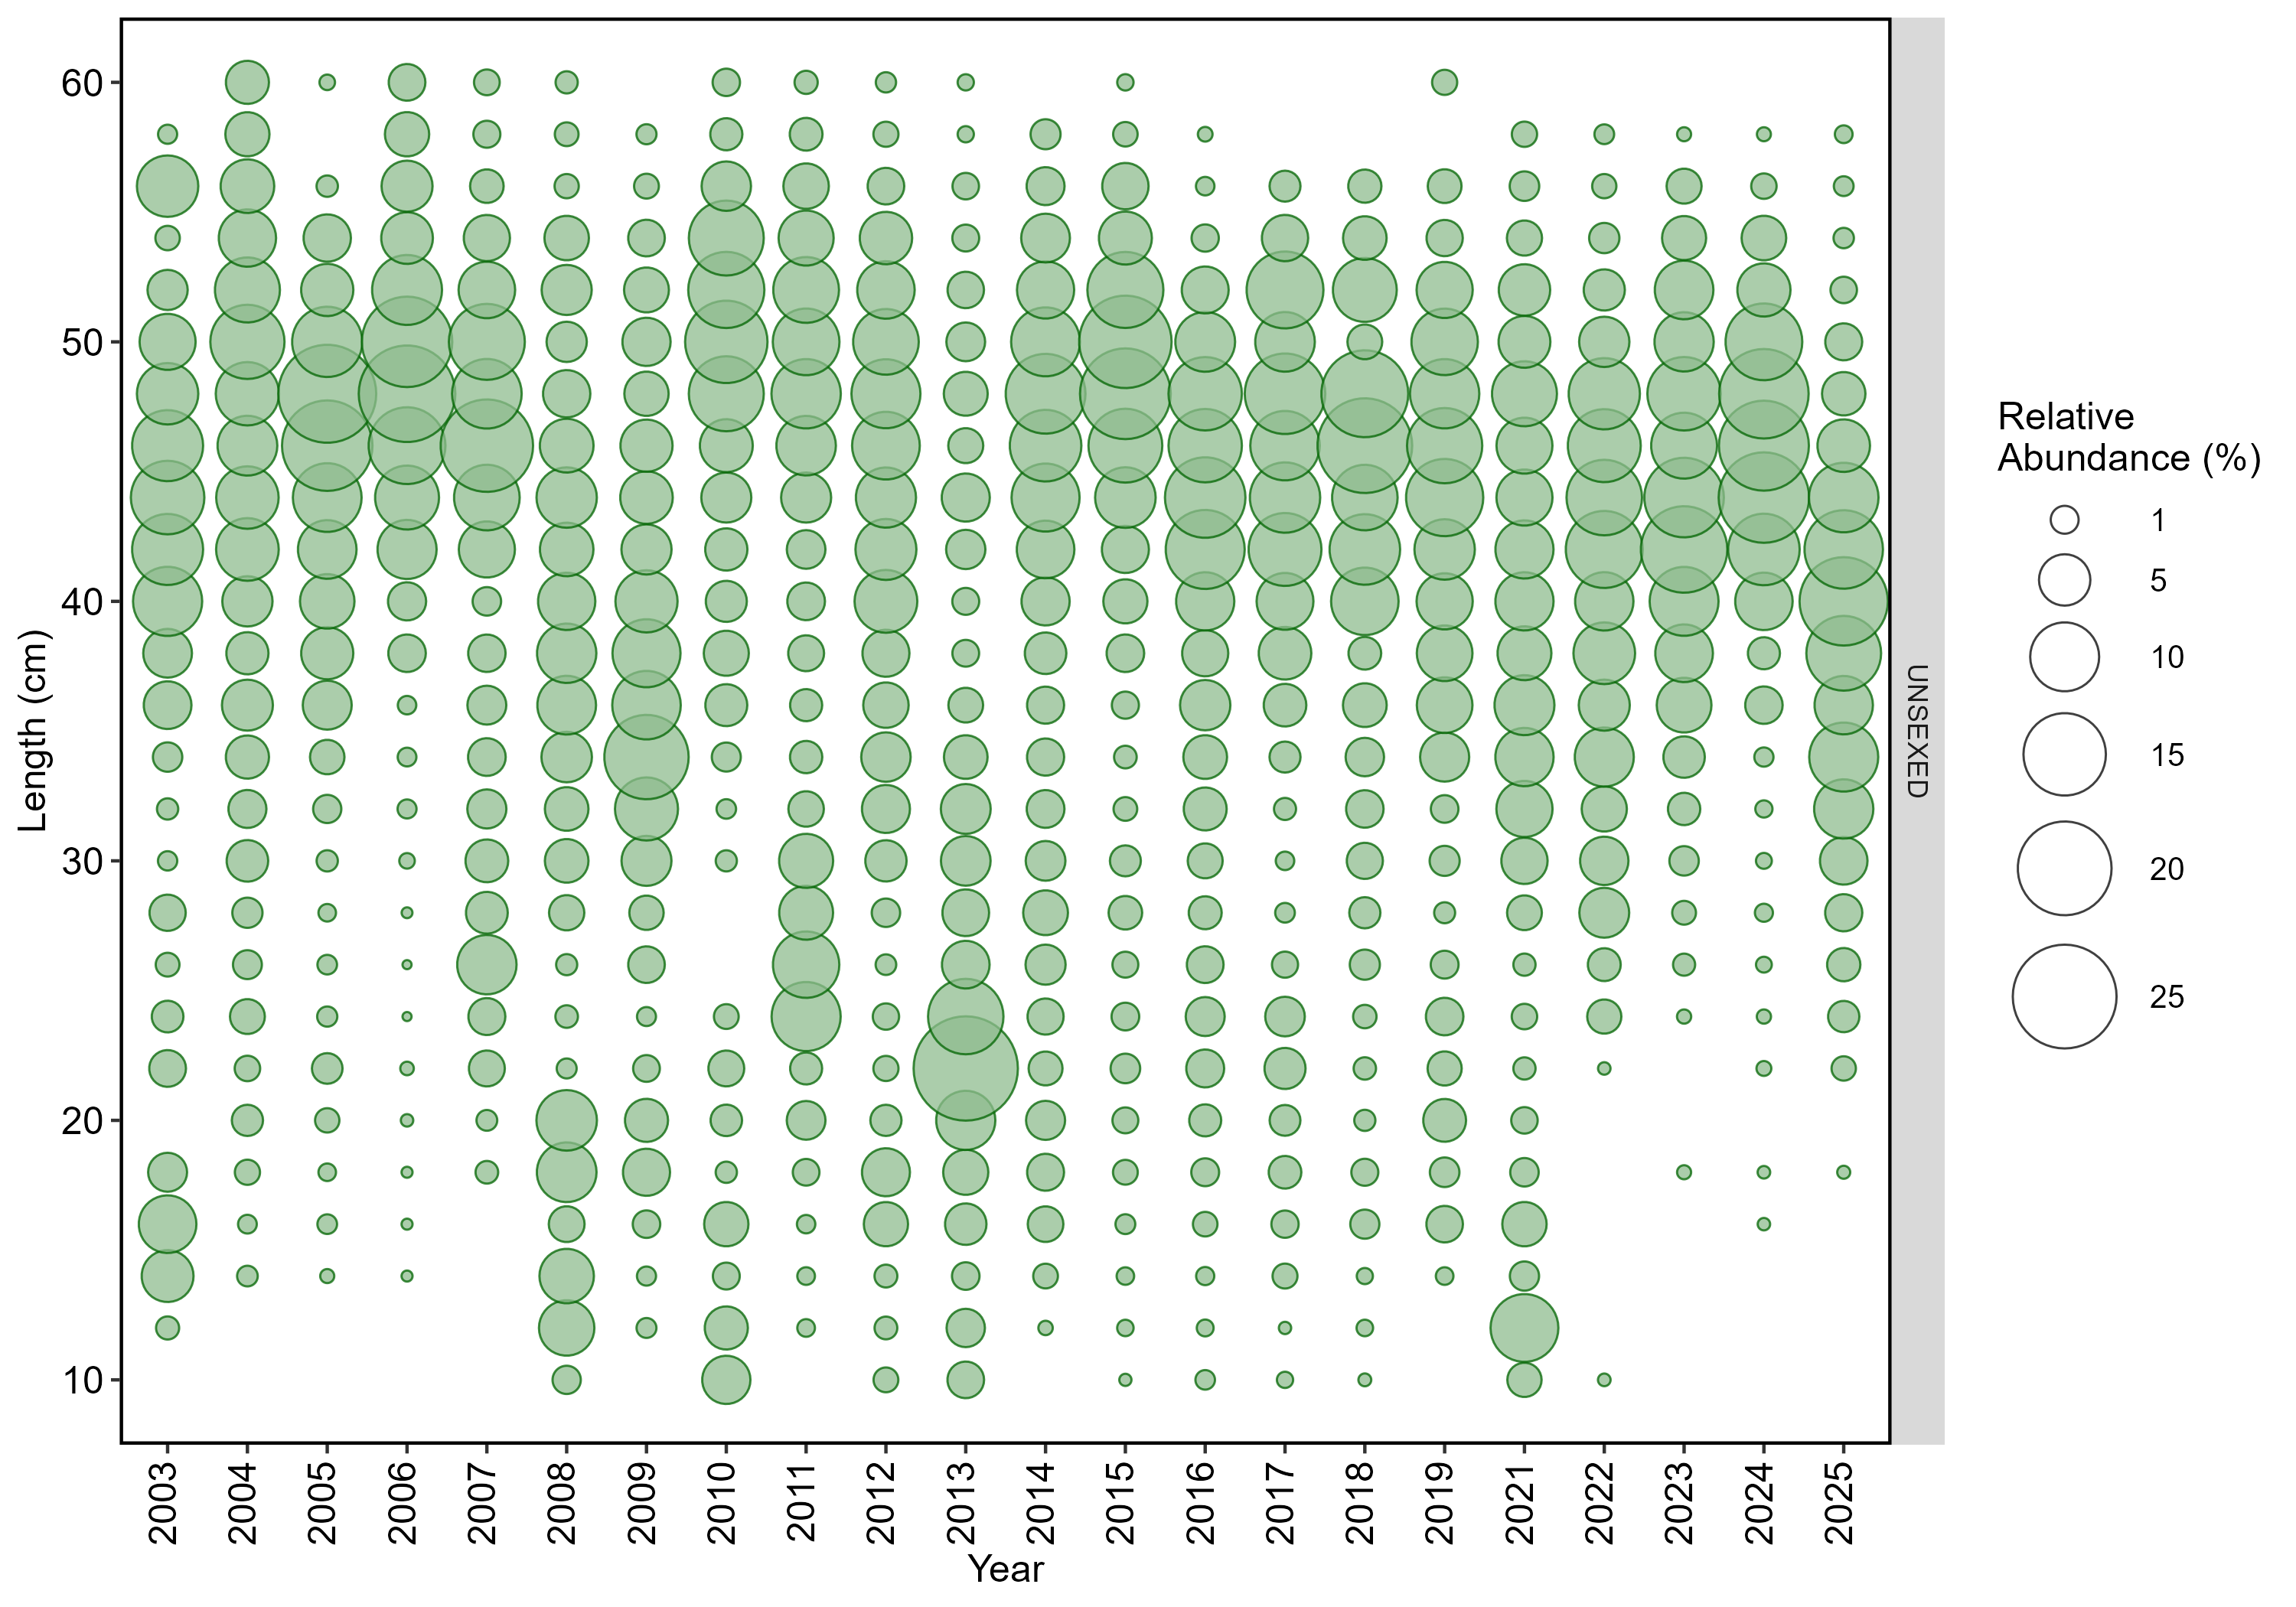
\includegraphics[width=0.95\linewidth,height=\textheight,keepaspectratio]{../plots/wcgbts_comps/plots/canary rockfish_length_frequency_sex_0.png}

}

\caption{Length (cm) compostion data from the NWFSC WCGBTS for canary
rockfish. Size of the circles within a year indicate higher (larger
circles) and lower (smaller circles) proportion observed by length bin.}

\end{figure}%

\newpage{}

\subsection{Chilipepper}\label{chilipepper}

The most recent assessment of chilipepper was a benchmark assessment
conducted in 2025. Across available data, chilipepper have been observed
and sampled by both the NWFSC HKLS and WCGBTS. The NWFSC HKLS observed
chilipepper at an average of 27 sets per year. The NWFSC WCGBTS observed
chilipepper on an average of 93 tows per year. For this species, a total
of 157 maturity samples have been collected coastwide (regardless of
stock area), with 157 read maturities.

\begingroup\fontsize{10}{12}\selectfont
\begingroup\fontsize{10}{12}\selectfont

\begin{longtable}[t]{>{\raggedleft\arraybackslash}p{2cm}>{\raggedleft\arraybackslash}p{3.5cm}>{\raggedleft\arraybackslash}p{2cm}>{\raggedleft\arraybackslash}p{2cm}>{\raggedleft\arraybackslash}p{2cm}}
\caption{\label{tab:unnamed-chunk-141}Total number of available lengths, read ages, and unread age structures by data source and
state for chilipepper.}\\
\toprule
State & Source & Lengths & Ages & Age Structures\\
\midrule
\endfirsthead
\caption[]{Total number of available lengths, read ages, and unread age structures by data source and
state for chilipepper. (\textit{continued)}}\\
\toprule
State & Source & Lengths & Ages & Age Structures\\
\midrule
\endhead

\endfoot
\bottomrule
\endlastfoot
CA & NWFSC HKLS & 3,335 & 249 & 2,903\\
CA & NWFSC WCGBTS & 35,095 & 12,386 & 1,480\\
OR & NWFSC WCGBTS & 2,231 & 904 & 89\\
WA & NWFSC WCGBTS & 34 & 27 & 7\\*
\end{longtable}
\endgroup{}
\endgroup{}

\begin{figure}[H]

{\centering 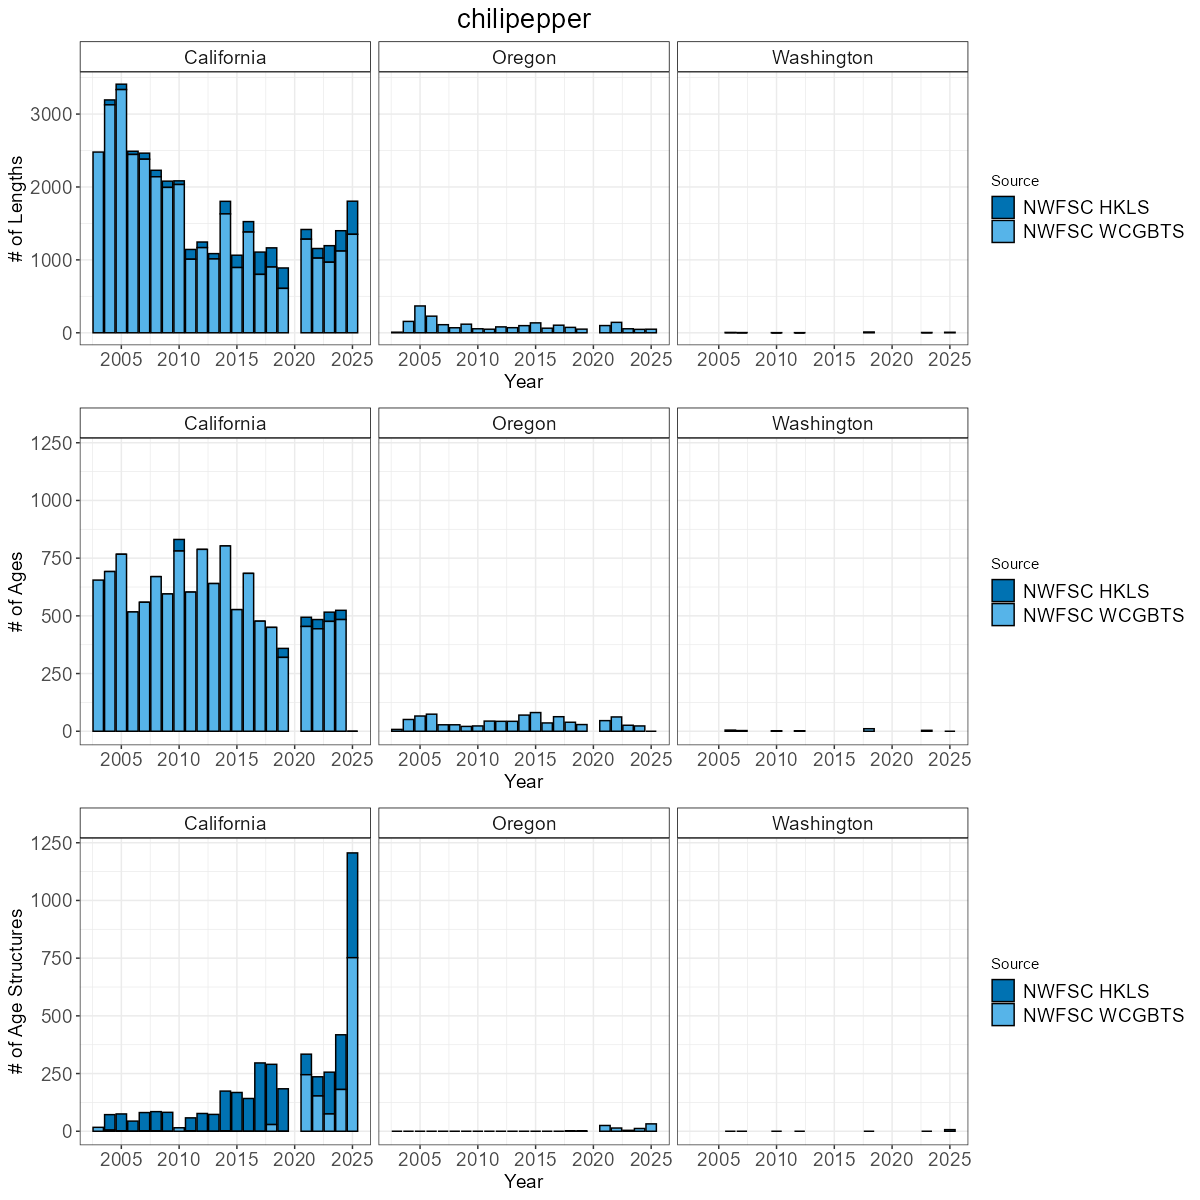
\includegraphics[width=0.95\linewidth,height=\textheight,keepaspectratio]{../plots/state_comparisons/chilipepper_state_compositions.png}

}

\caption{Total number of available lengths, read ages, and unread age
structures by data source by year for chilipepper. Note the y-axis
maximum may differ by data type.}

\end{figure}%

\begin{figure}[H]

{\centering 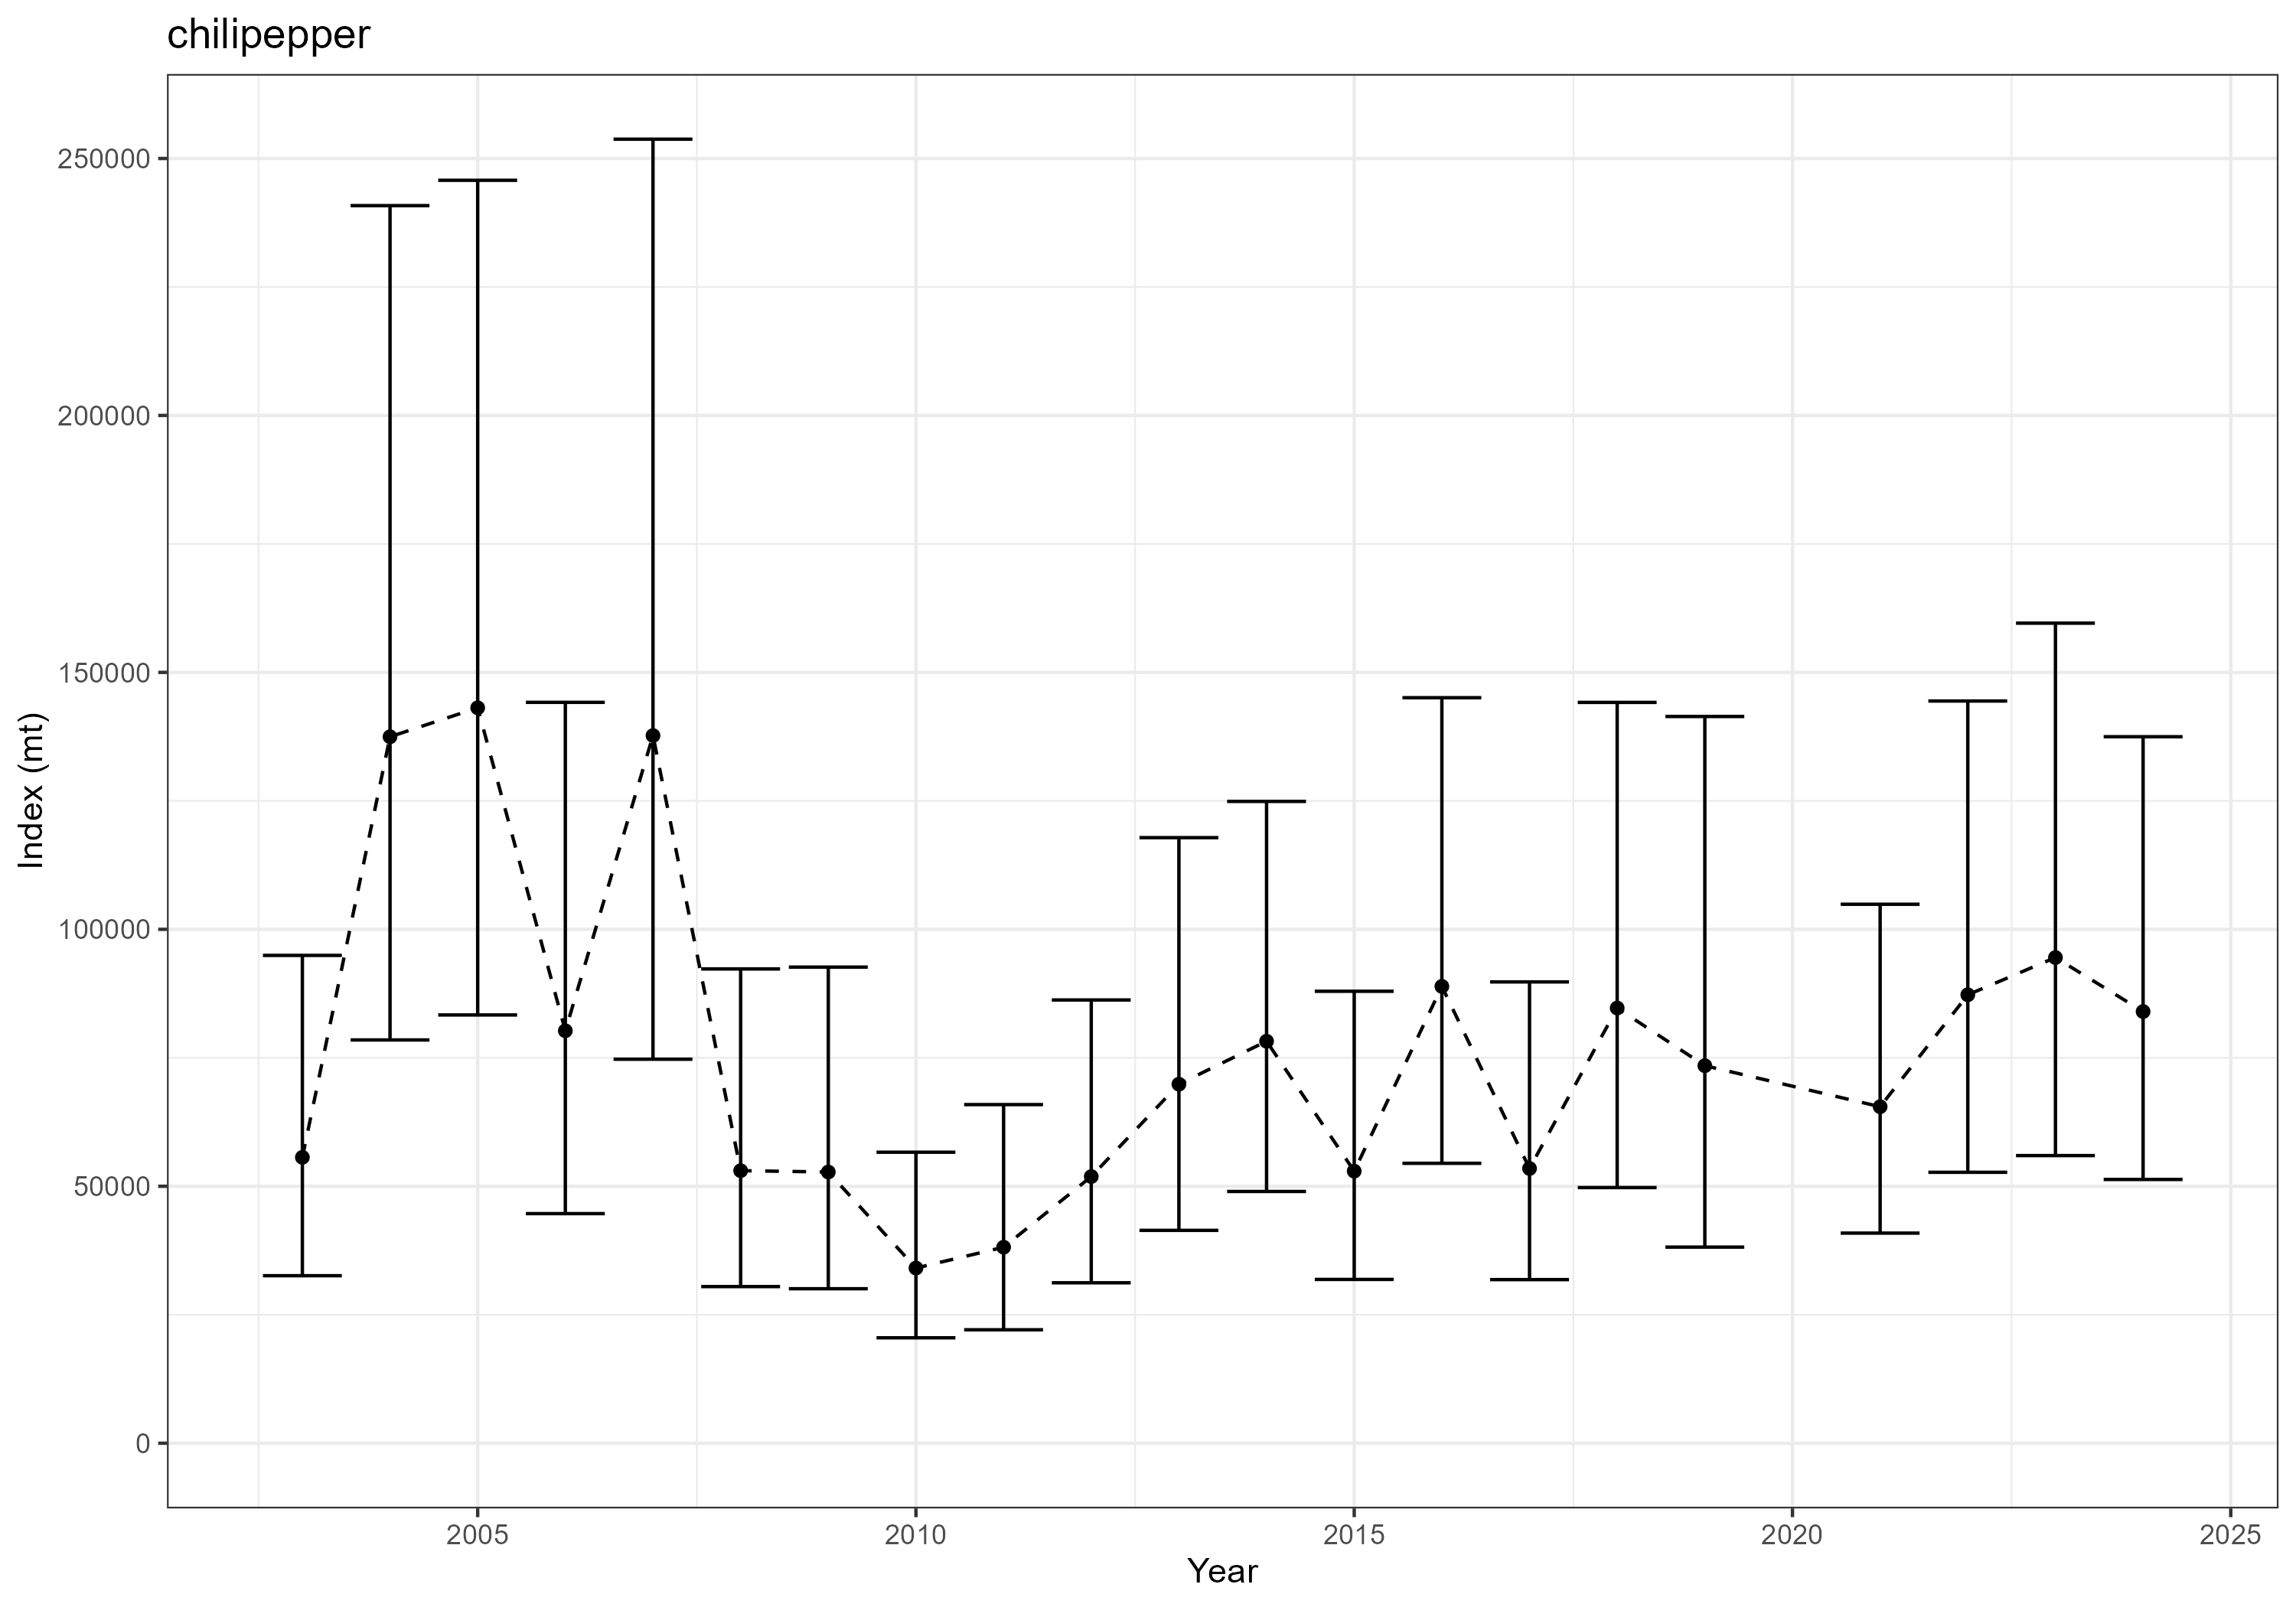
\includegraphics[width=0.95\linewidth,height=\textheight,keepaspectratio]{../plots/wcgbts_indices/chilipepper_index.png}

}

\caption{Estimated relative index of abundance for chilipepper from the
NWFSC WCGBTS.}

\end{figure}%

\begin{figure}[H]

{\centering 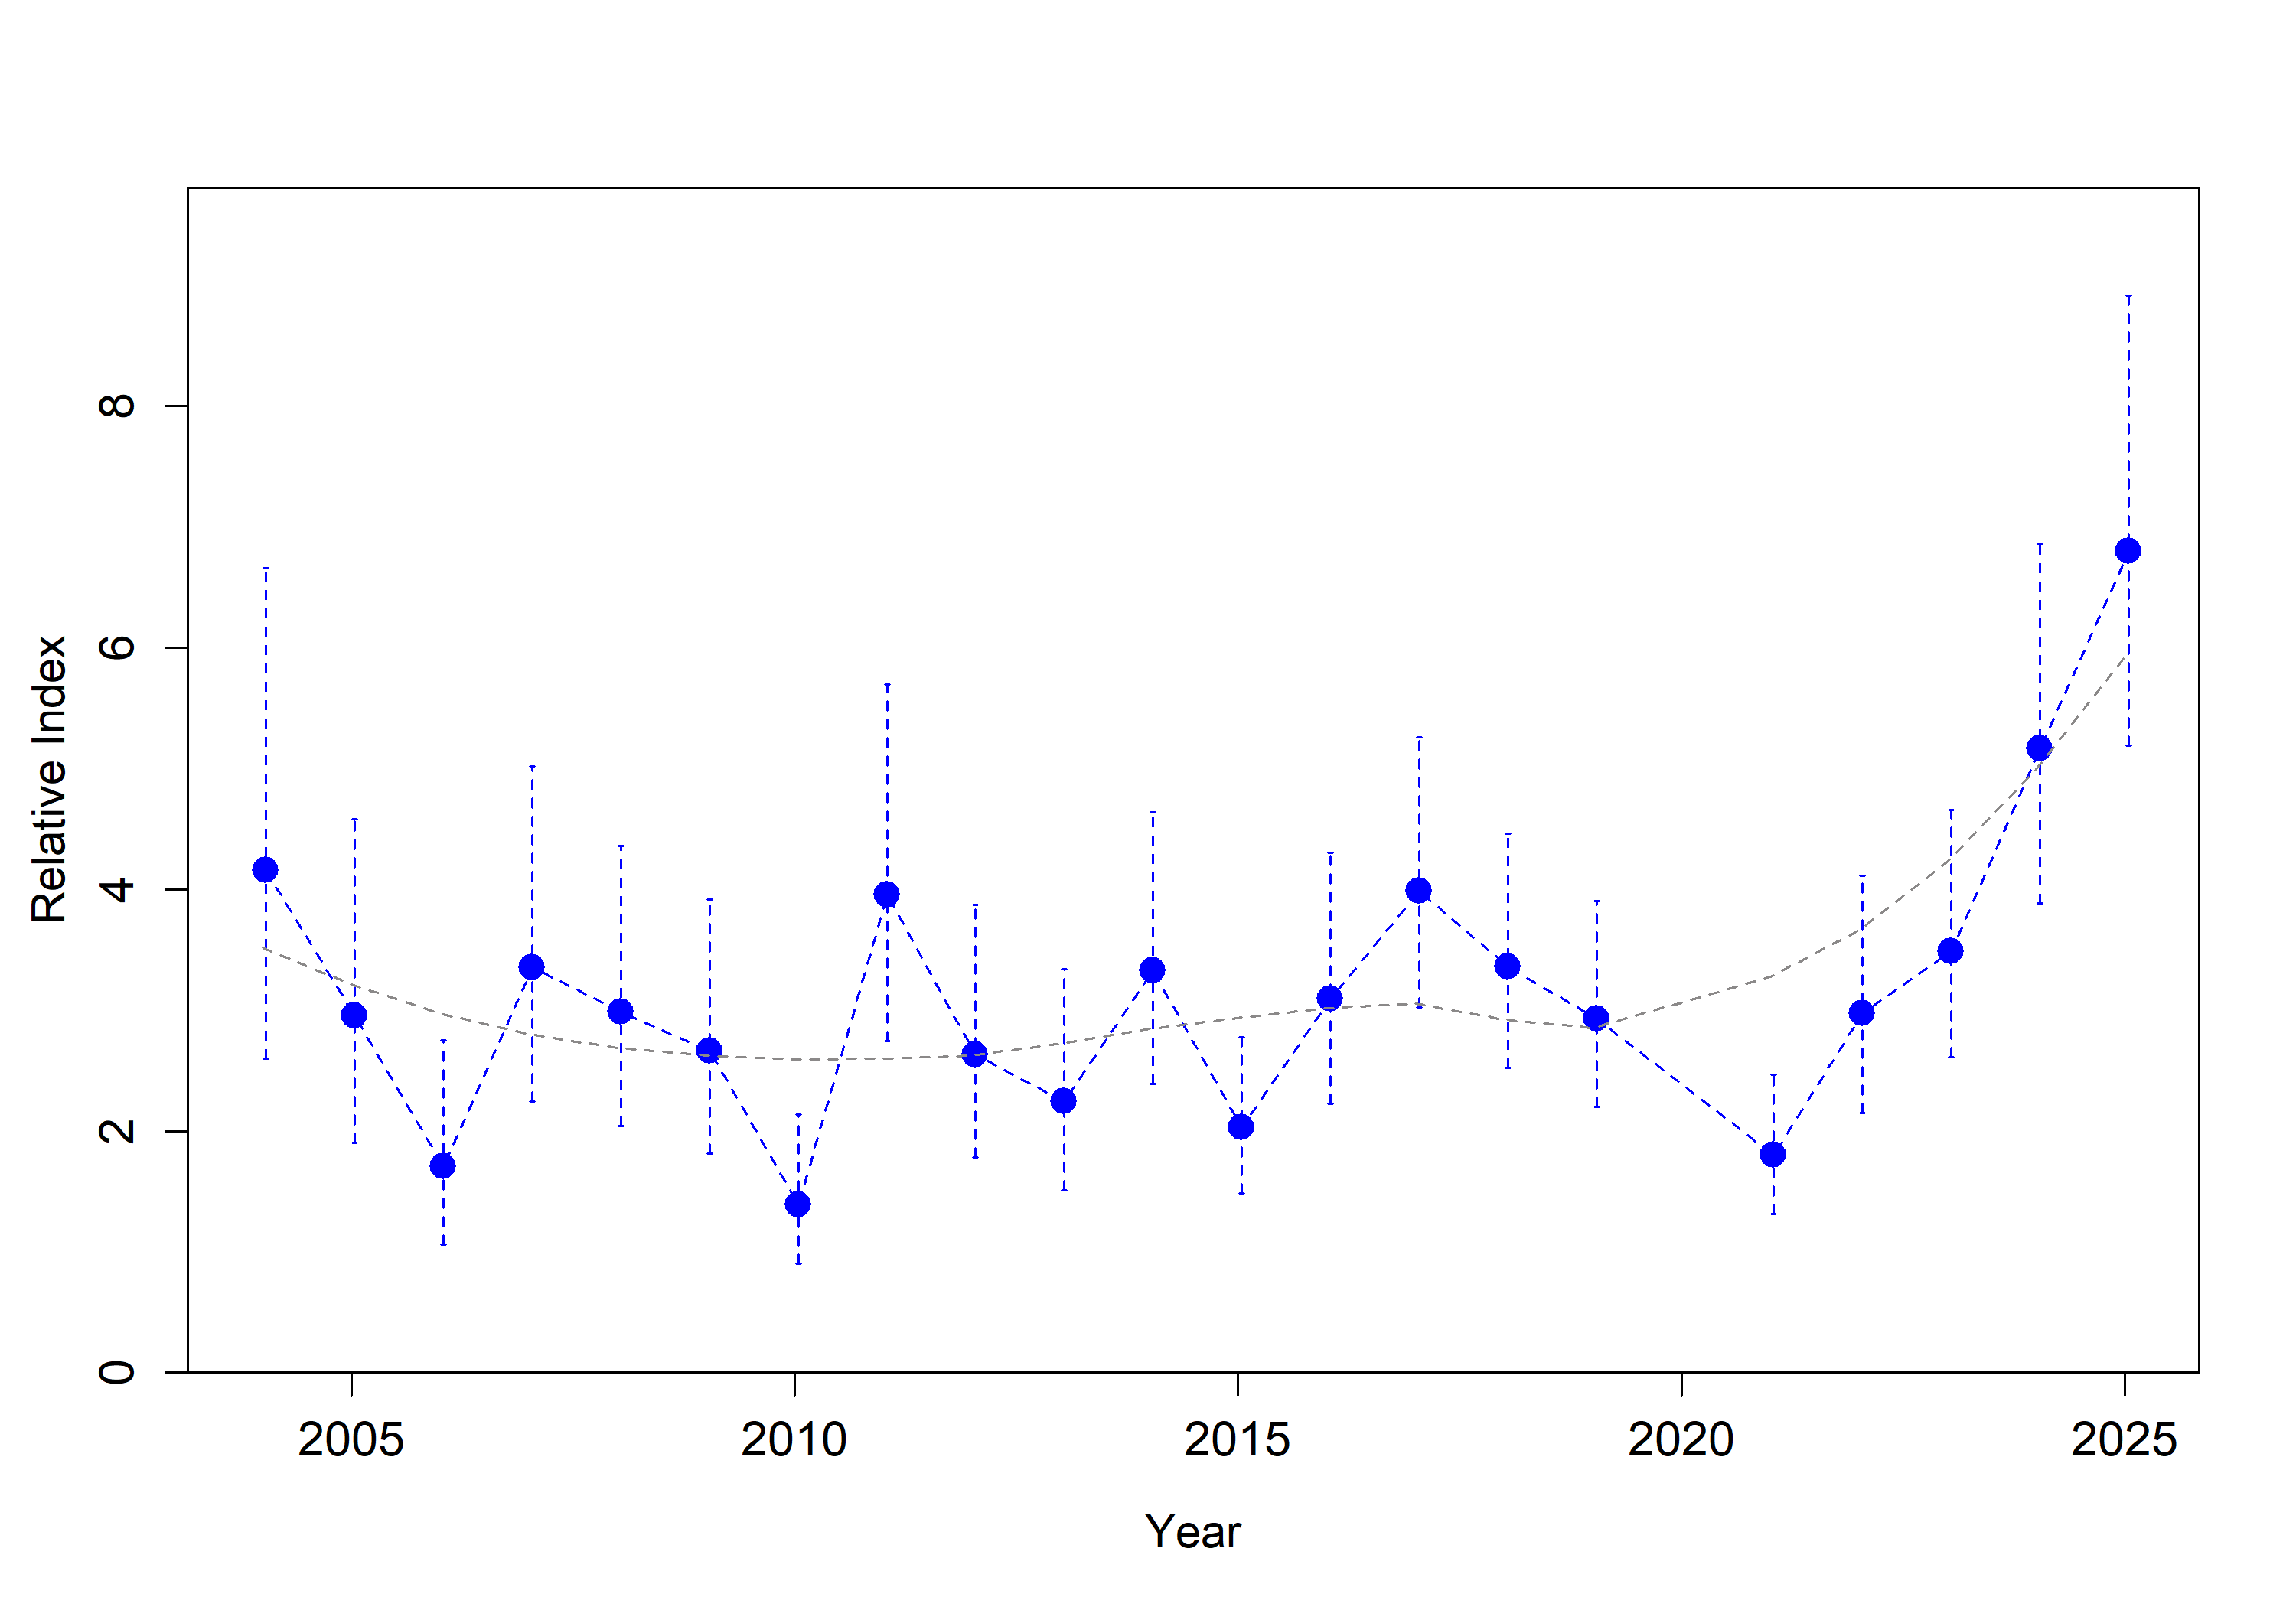
\includegraphics[width=0.95\linewidth,height=\textheight,keepaspectratio]{../plots/hkl_indices/chilipepper_negbinom index.png}

}

\caption{Estimated relative index of abundance for chilipepper from the
NWFSC HKLS.}

\end{figure}%

\begin{figure}[H]

{\centering 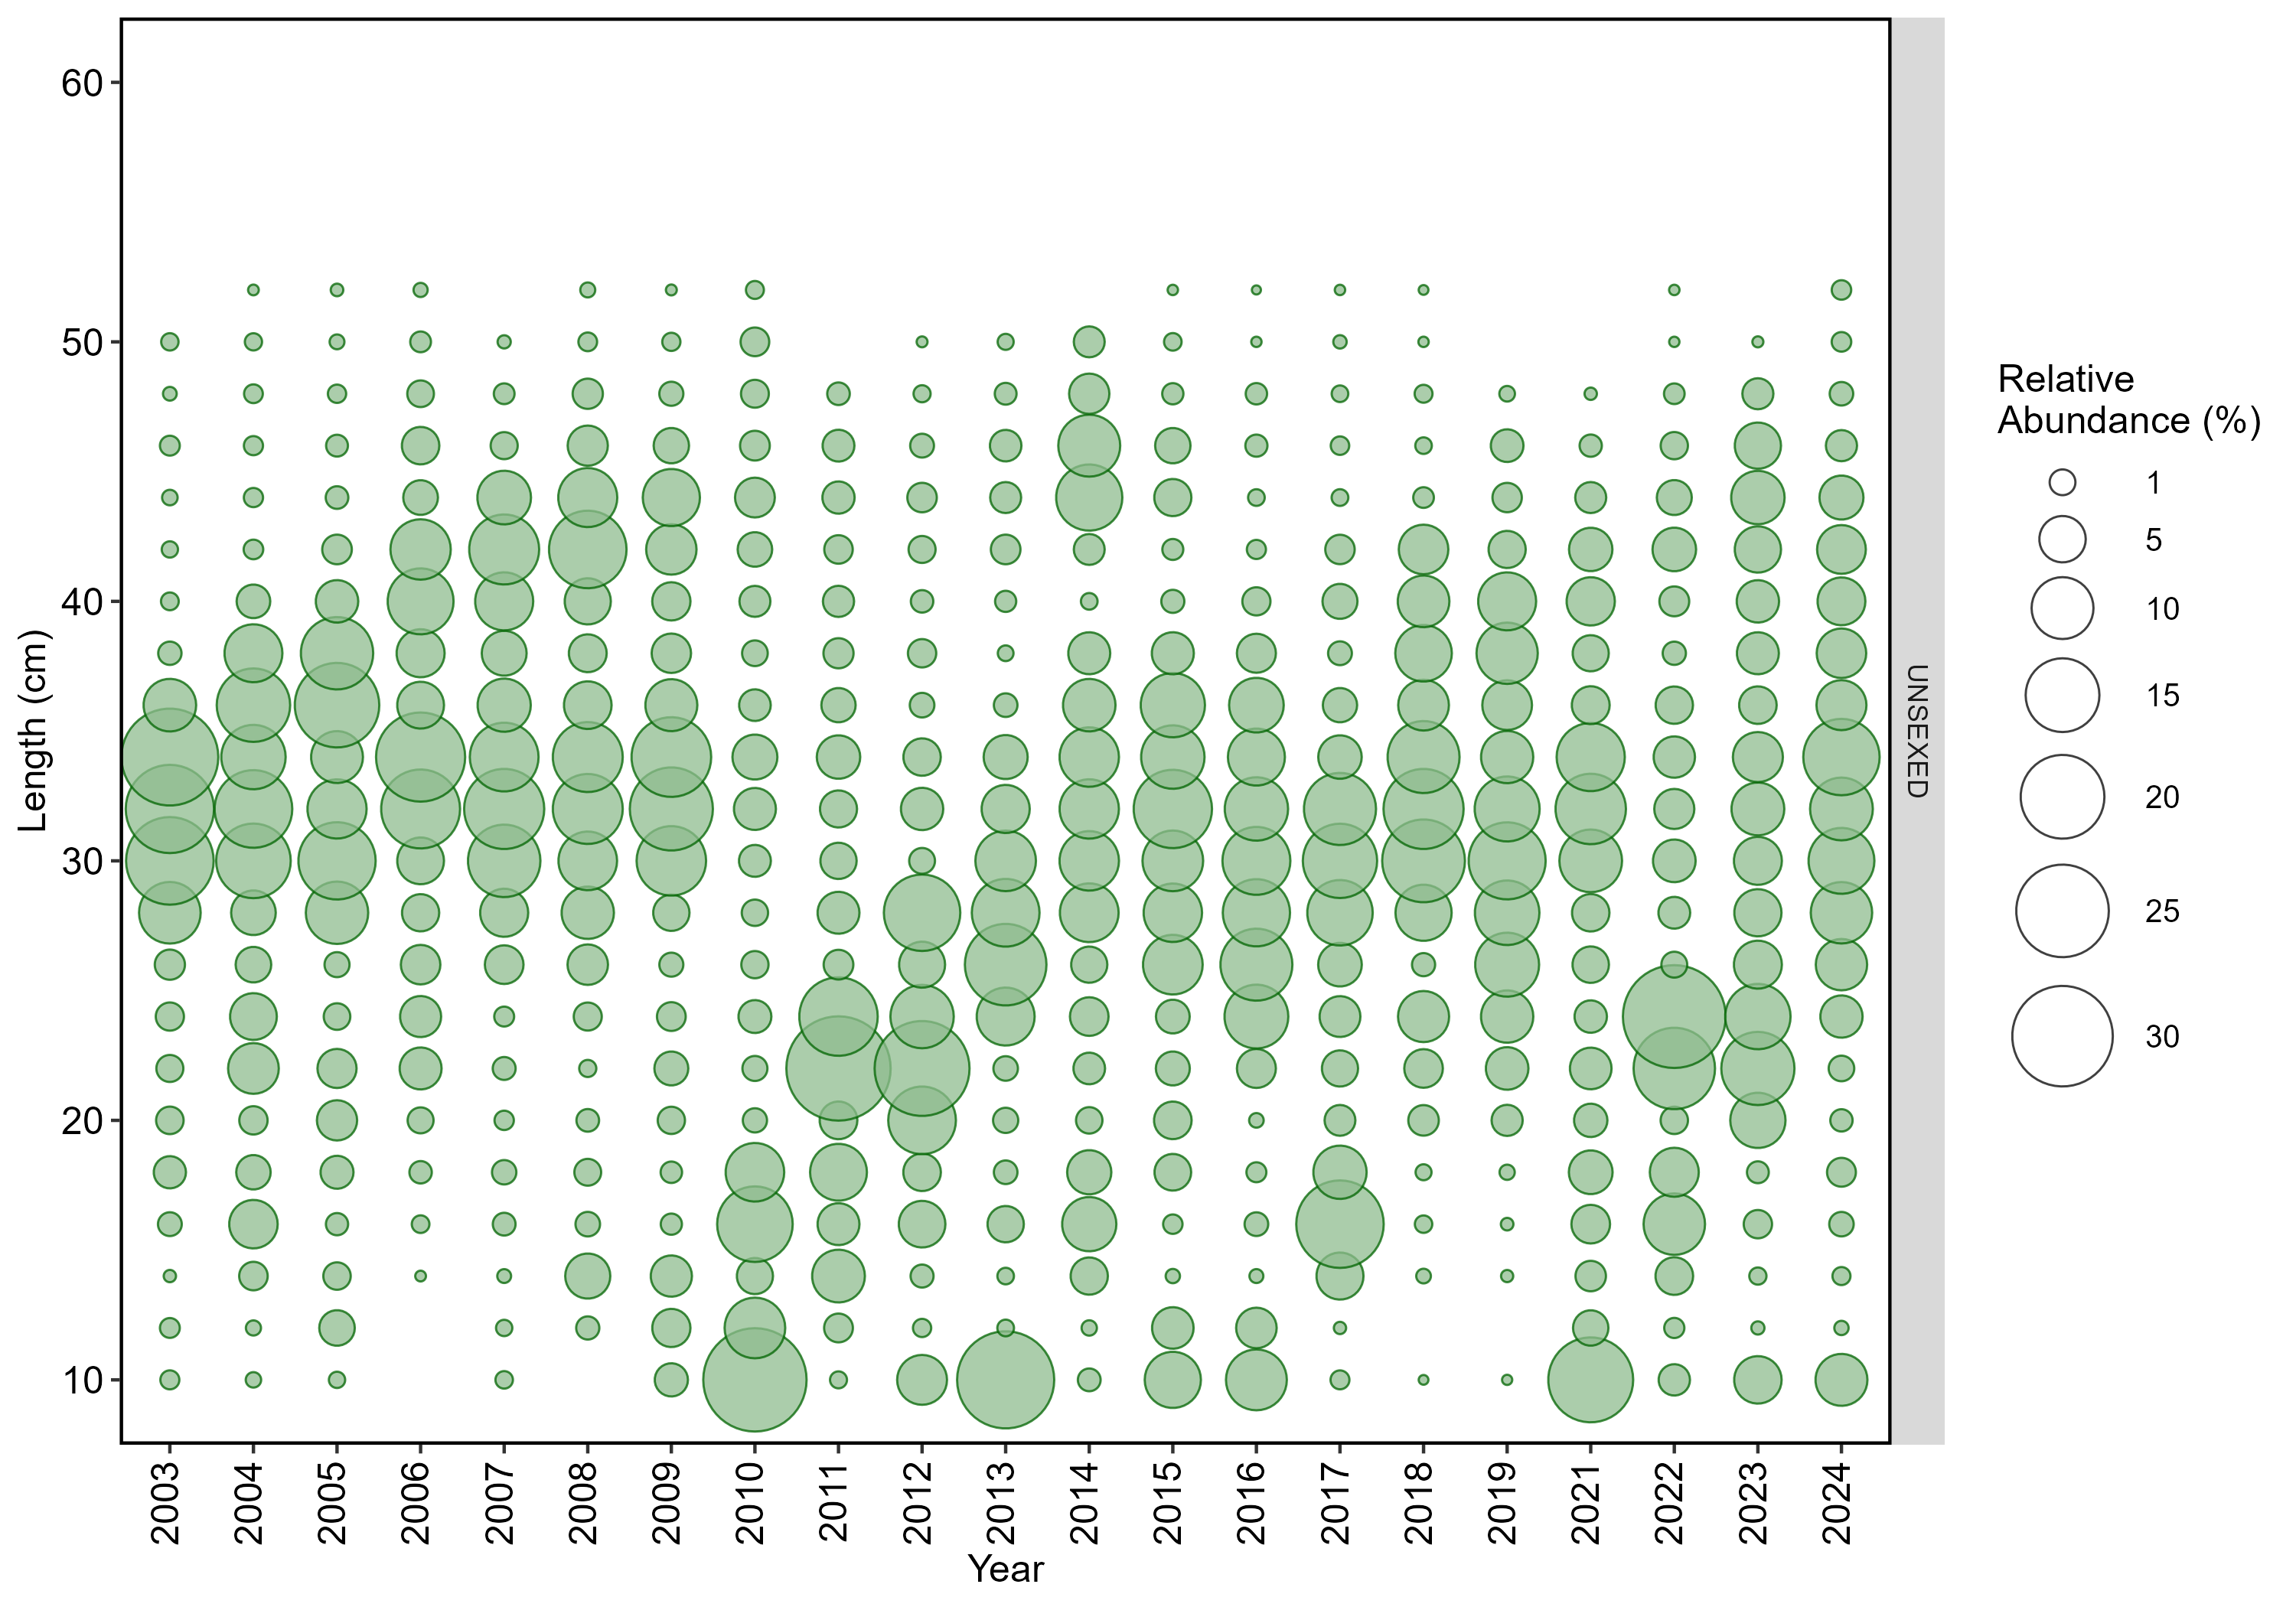
\includegraphics[width=0.95\linewidth,height=\textheight,keepaspectratio]{../plots/wcgbts_comps/plots/chilipepper_length_frequency_sex_0.png}

}

\caption{Length (cm) compostion data from the NWFSC WCGBTS for
chilipepper. Size of the circles within a year indicate higher (larger
circles) and lower (smaller circles) proportion observed by length bin.}

\end{figure}%

\begin{figure}[H]

{\centering 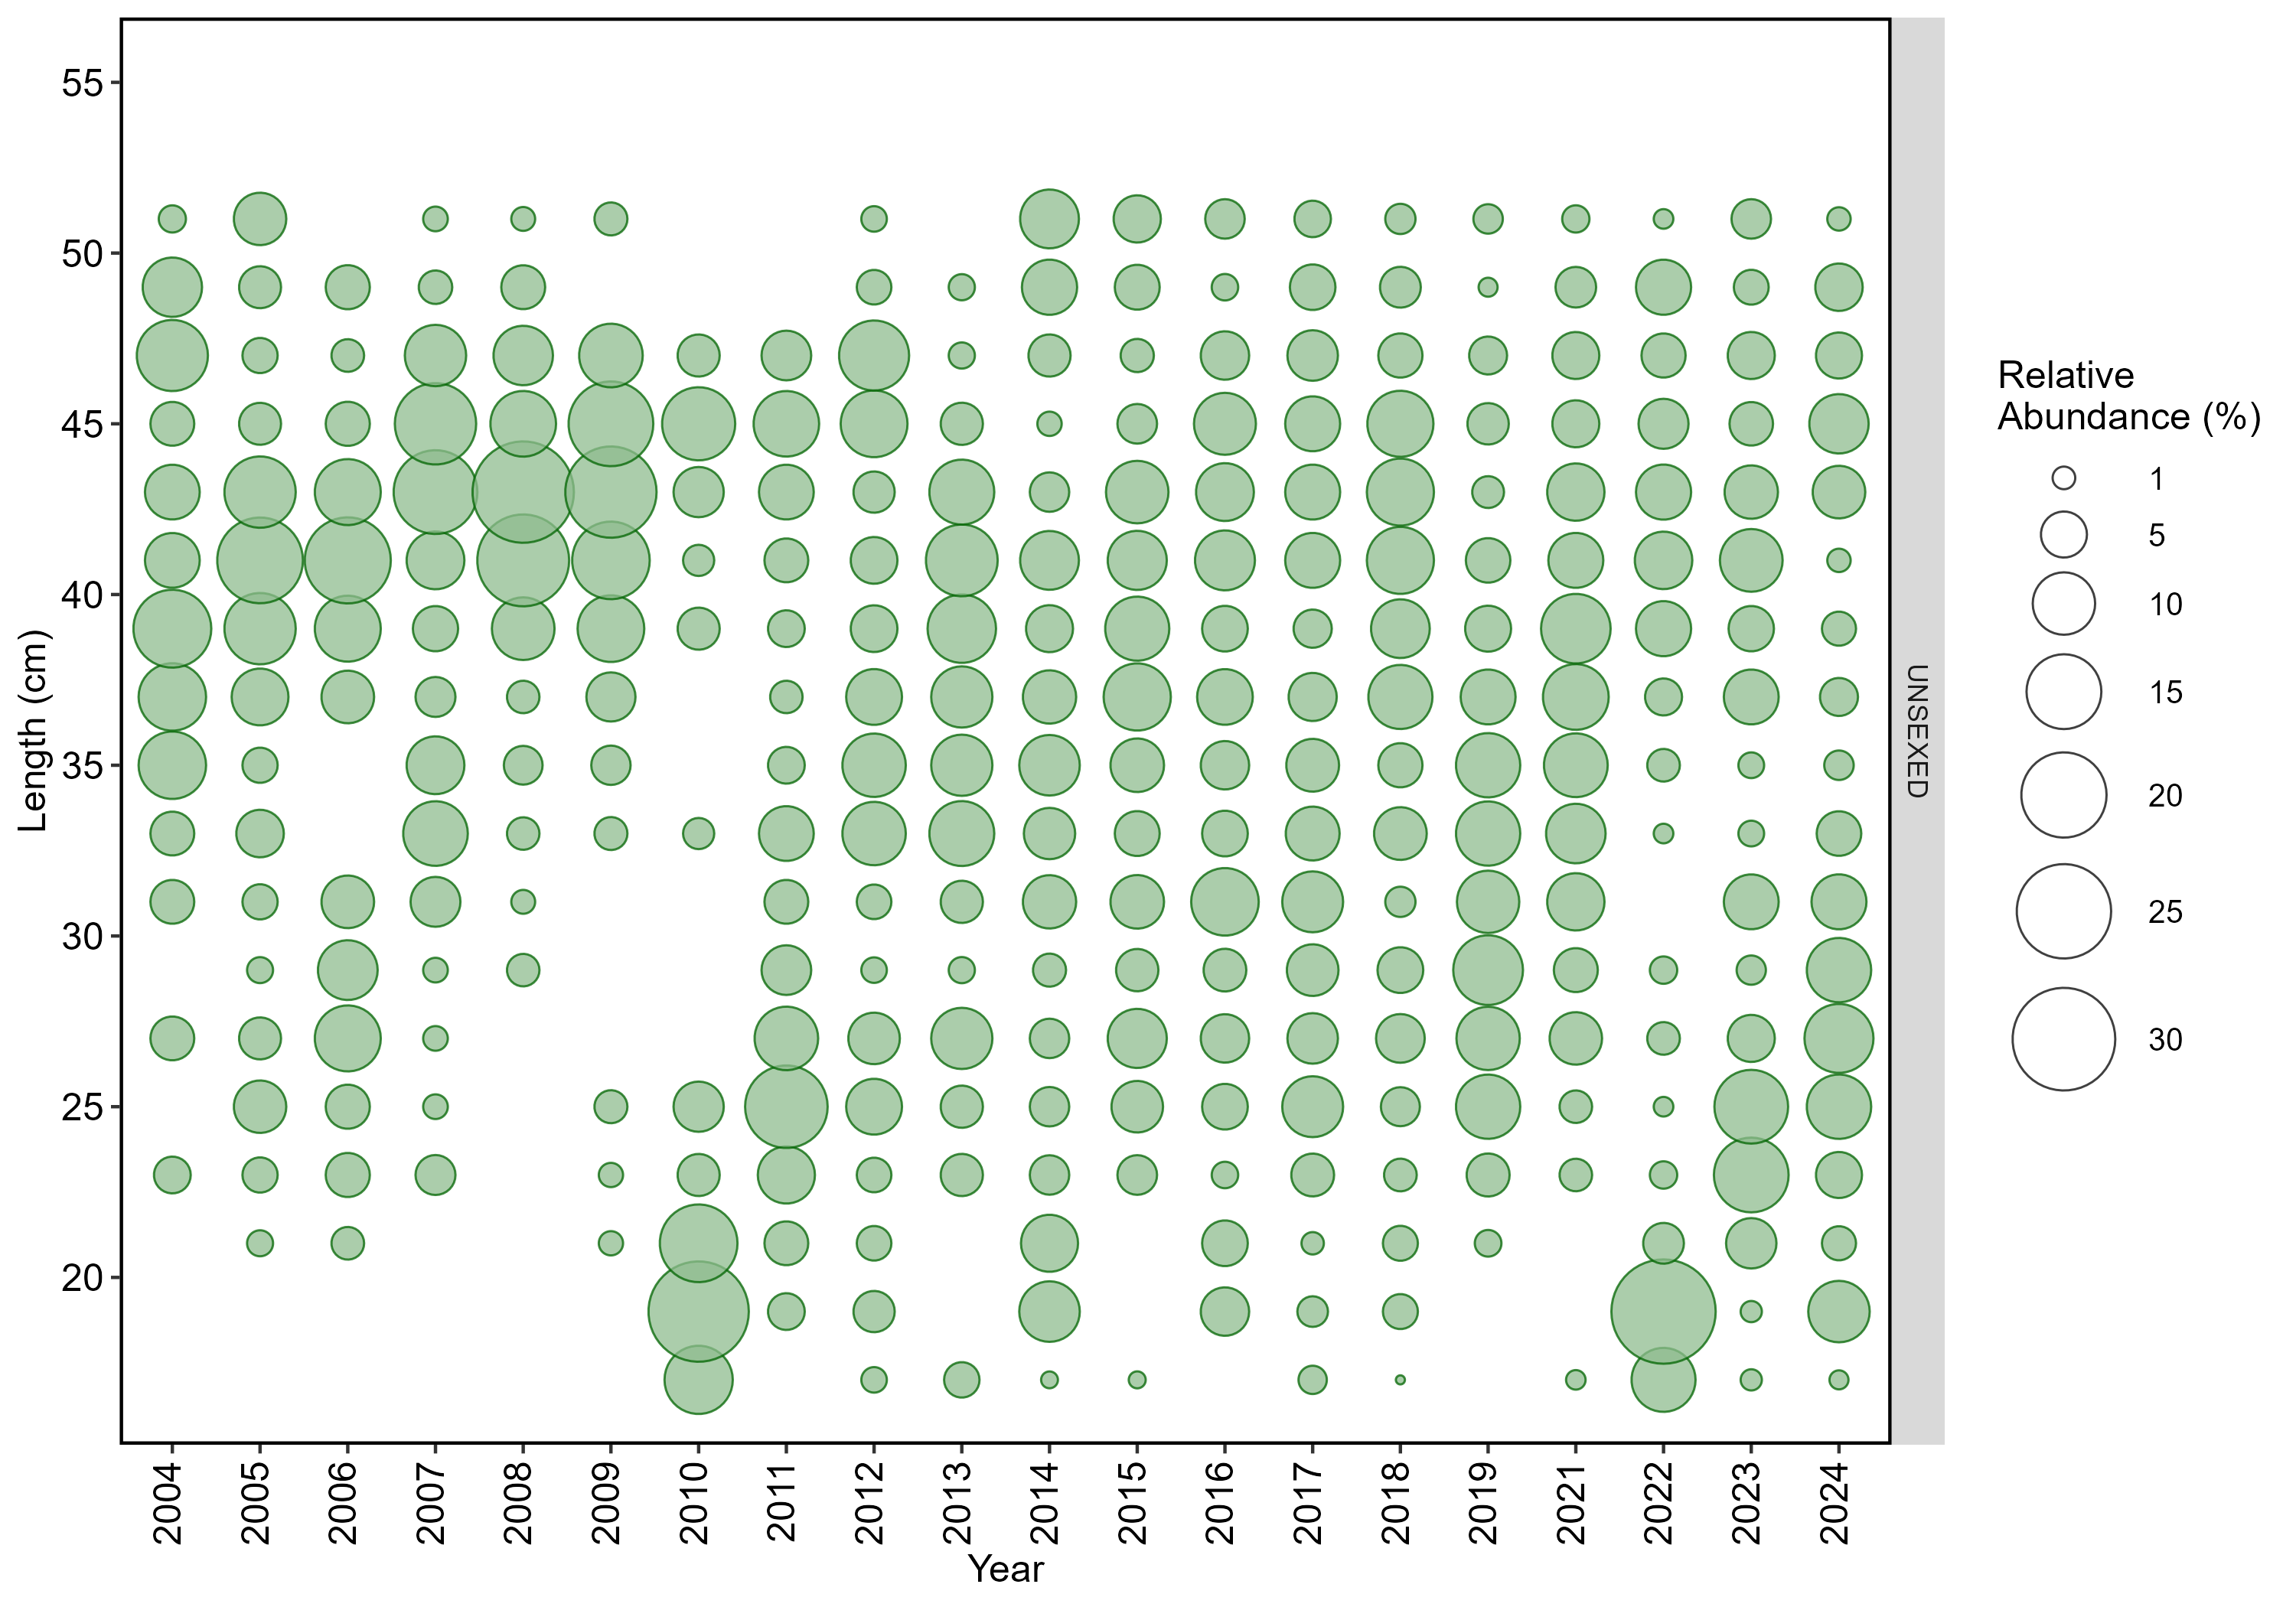
\includegraphics[width=0.95\linewidth,height=\textheight,keepaspectratio]{../plots/hkl_comps/plots/chilipepper_nwfsc_hkl_length_frequency_sex_0.png}

}

\caption{Length (cm) compostion data from the NWFSC HKLS for
chilipepper. Size of the circles within a year indicate higher (larger
circles) and lower (smaller circles) proportion observed by length bin.}

\end{figure}%

\newpage{}

\subsection{Cowcod}\label{cowcod}

The most recent assessment of cowcod was a benchmark assessment
conducted in 2019. Across available data, cowcod have been observed and
sampled by both the NWFSC HKLS and WCGBTS. The NWFSC HKLS observed
cowcod at an average of 24 sets per year. The NWFSC WCGBTS observed
cowcod on an average of 20 tows per year. For this species, a total of
431 maturity samples have been collected coastwide (regardless of stock
area), with 170 read maturities.

\begingroup\fontsize{10}{12}\selectfont
\begingroup\fontsize{10}{12}\selectfont

\begin{longtable}[t]{>{\raggedleft\arraybackslash}p{2cm}>{\raggedleft\arraybackslash}p{3.5cm}>{\raggedleft\arraybackslash}p{2cm}>{\raggedleft\arraybackslash}p{2cm}>{\raggedleft\arraybackslash}p{2cm}}
\caption{\label{tab:unnamed-chunk-159}Total number of available lengths, read ages, and unread age structures by data source and
state for cowcod.}\\
\toprule
State & Source & Lengths & Ages & Age Structures\\
\midrule
\endfirsthead
\caption[]{Total number of available lengths, read ages, and unread age structures by data source and
state for cowcod. (\textit{continued)}}\\
\toprule
State & Source & Lengths & Ages & Age Structures\\
\midrule
\endhead

\endfoot
\bottomrule
\endlastfoot
CA & NWFSC HKLS & 1,099 & 440 & 629\\
CA & NWFSC WCGBTS & 1,038 & 465 & 560\\
OR & NWFSC WCGBTS & 10 & 3 & 7\\
WA & NWFSC WCGBTS & 2 & 0 & 2\\*
\end{longtable}
\endgroup{}
\endgroup{}

\begin{figure}[H]

{\centering 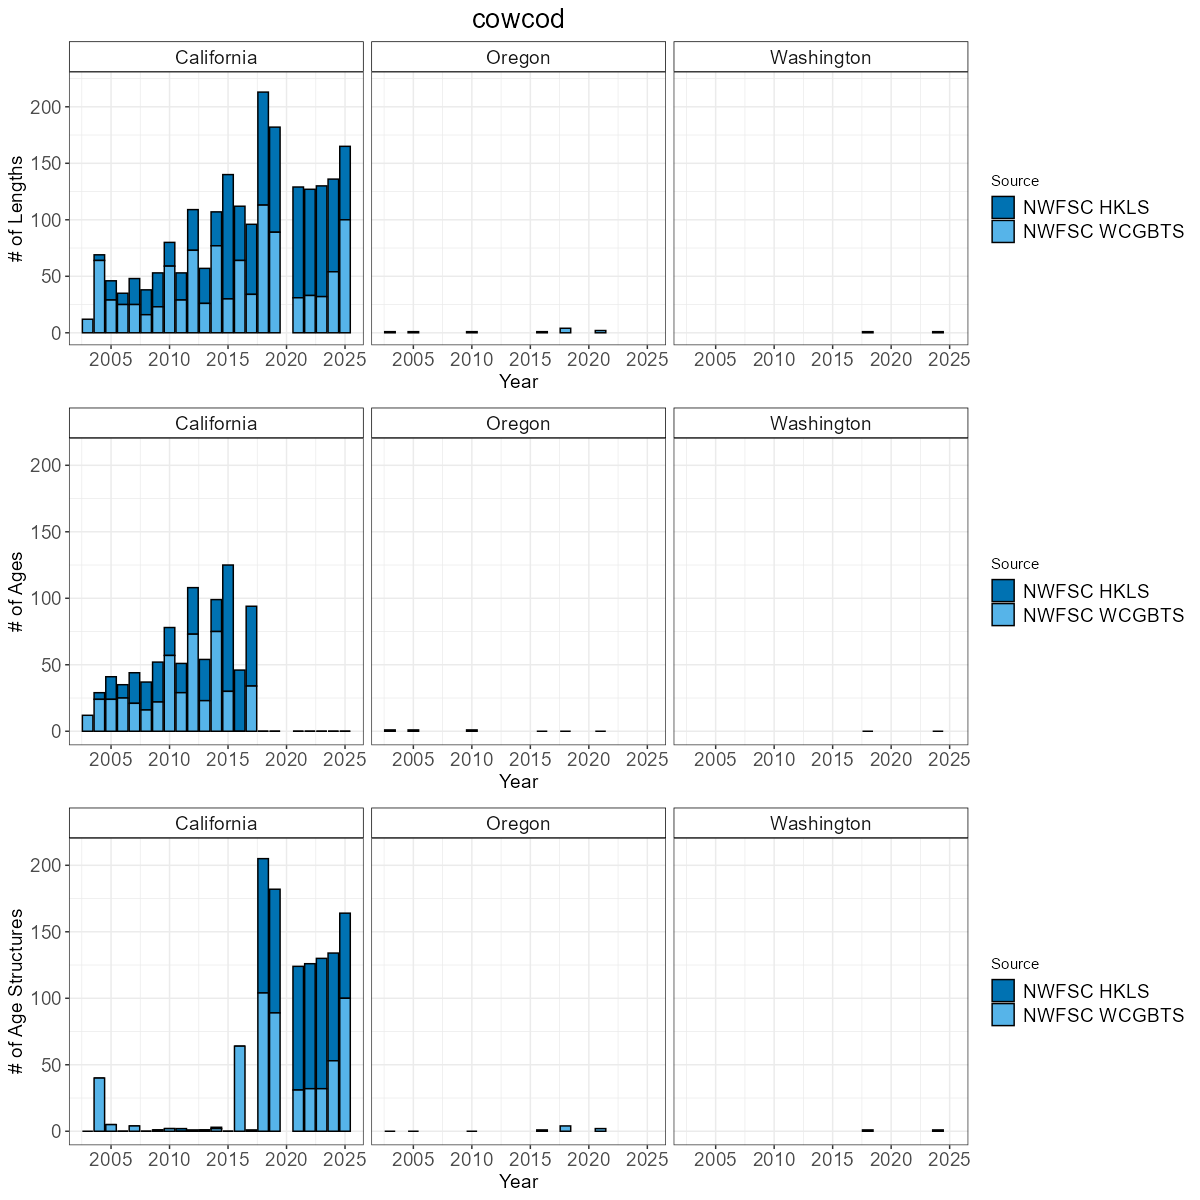
\includegraphics[width=0.95\linewidth,height=\textheight,keepaspectratio]{../plots/state_comparisons/cowcod_state_compositions.png}

}

\caption{Total number of available lengths, read ages, and unread age
structures by data source by year for cowcod. Note the y-axis maximum
may differ by data type.}

\end{figure}%

\begin{figure}[H]

{\centering 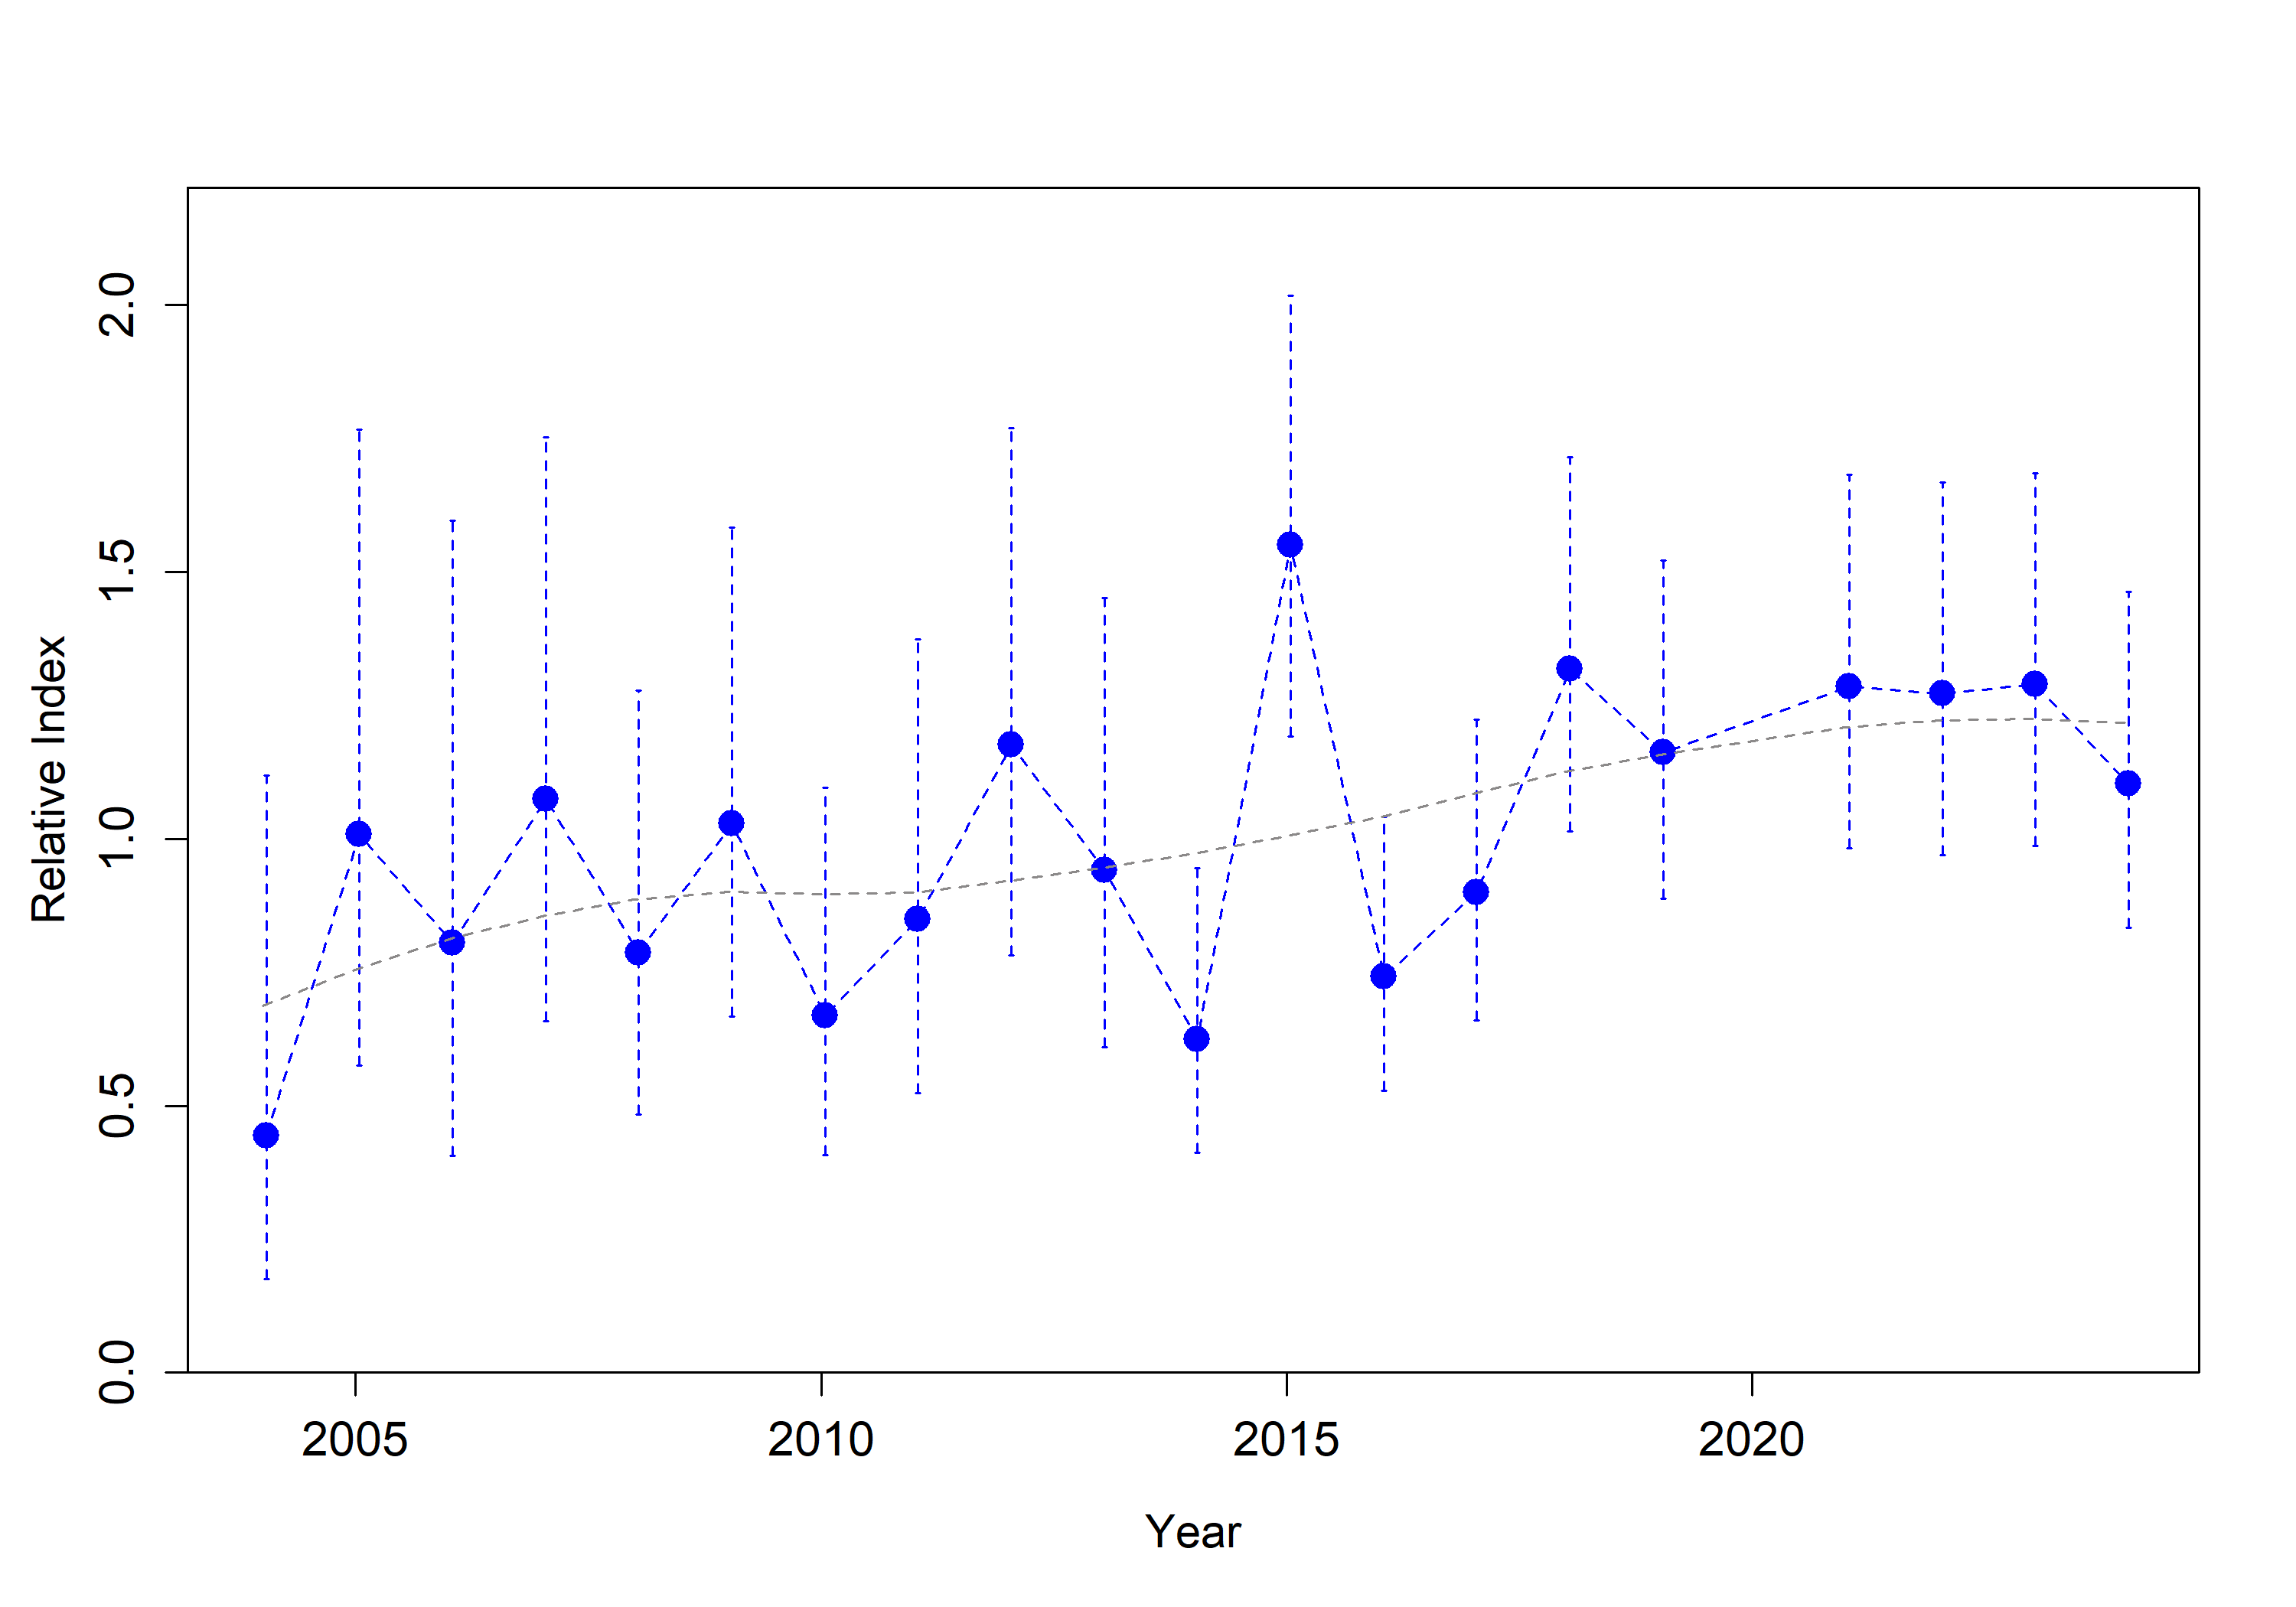
\includegraphics[width=0.95\linewidth,height=\textheight,keepaspectratio]{../plots/hkl_indices/cowcod_negbinom index.png}

}

\caption{Estimated relative index of abundance for cowcod from the NWFSC
HKLS.}

\end{figure}%

\begin{figure}[H]

{\centering 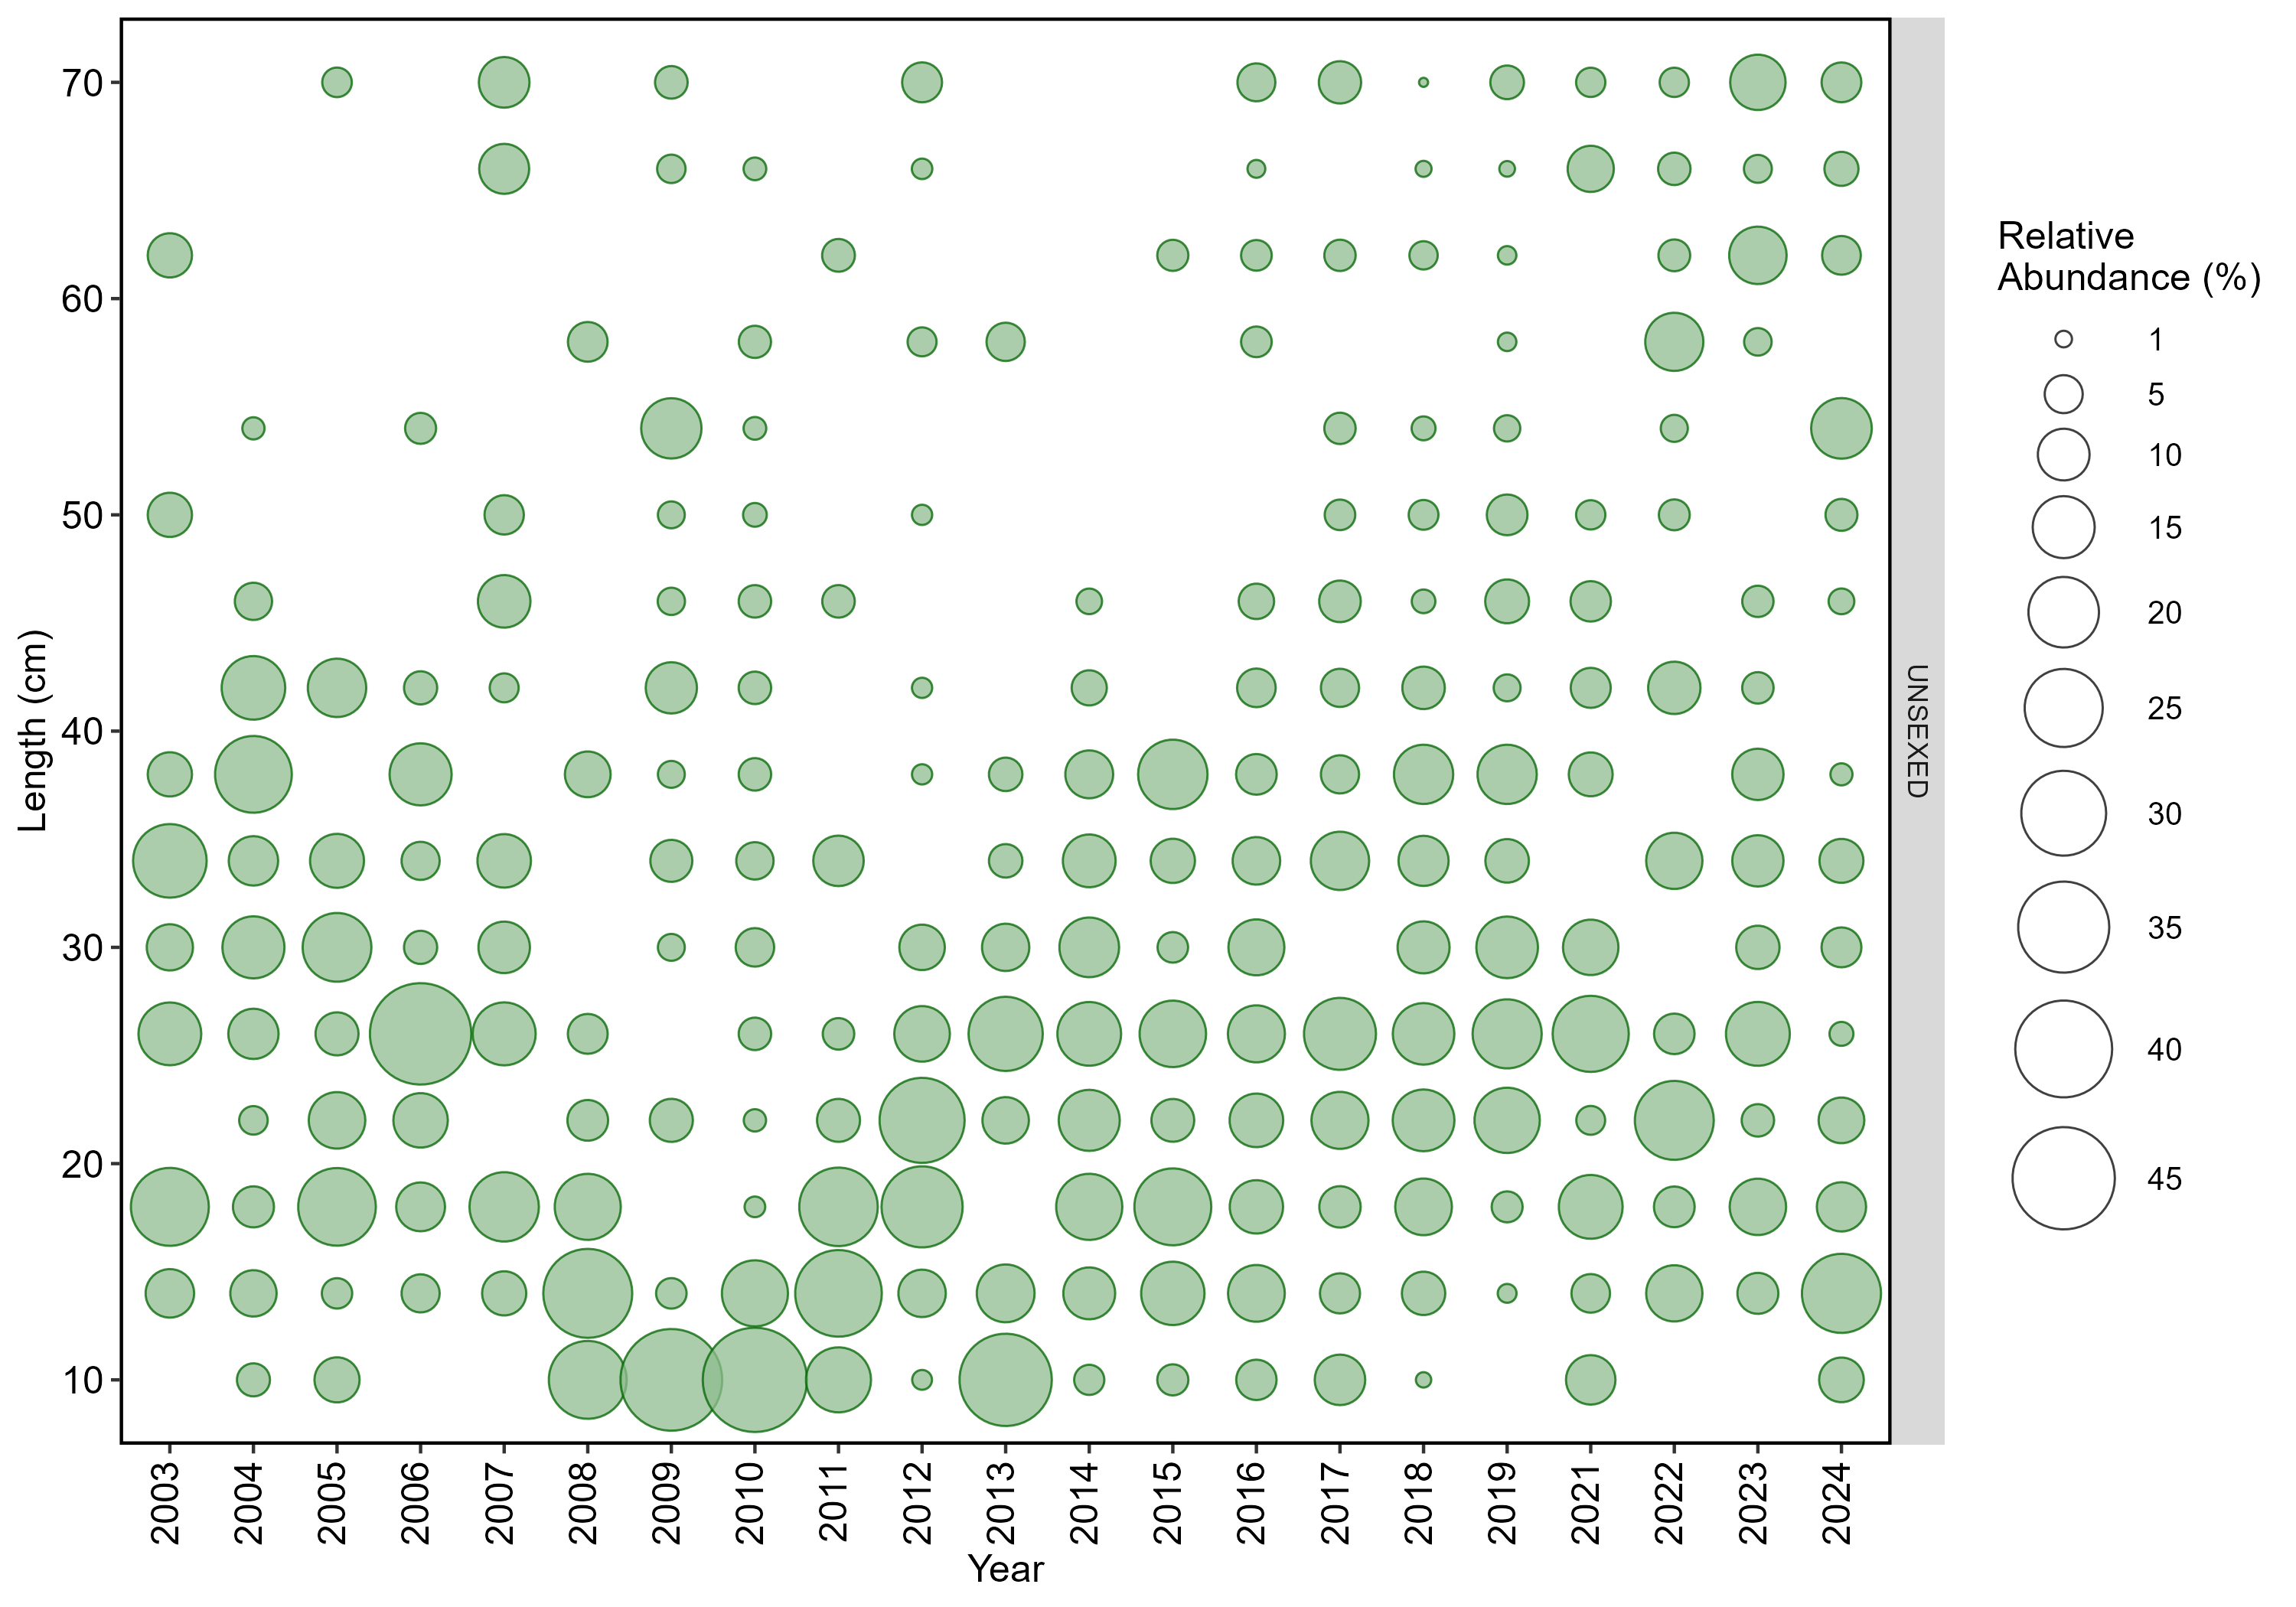
\includegraphics[width=0.95\linewidth,height=\textheight,keepaspectratio]{../plots/wcgbts_comps/plots/cowcod_length_frequency_sex_0.png}

}

\caption{Length (cm) compostion data from the NWFSC WCGBTS for cowcod.
Size of the circles within a year indicate higher (larger circles) and
lower (smaller circles) proportion observed by length bin.}

\end{figure}%

\begin{figure}[H]

{\centering 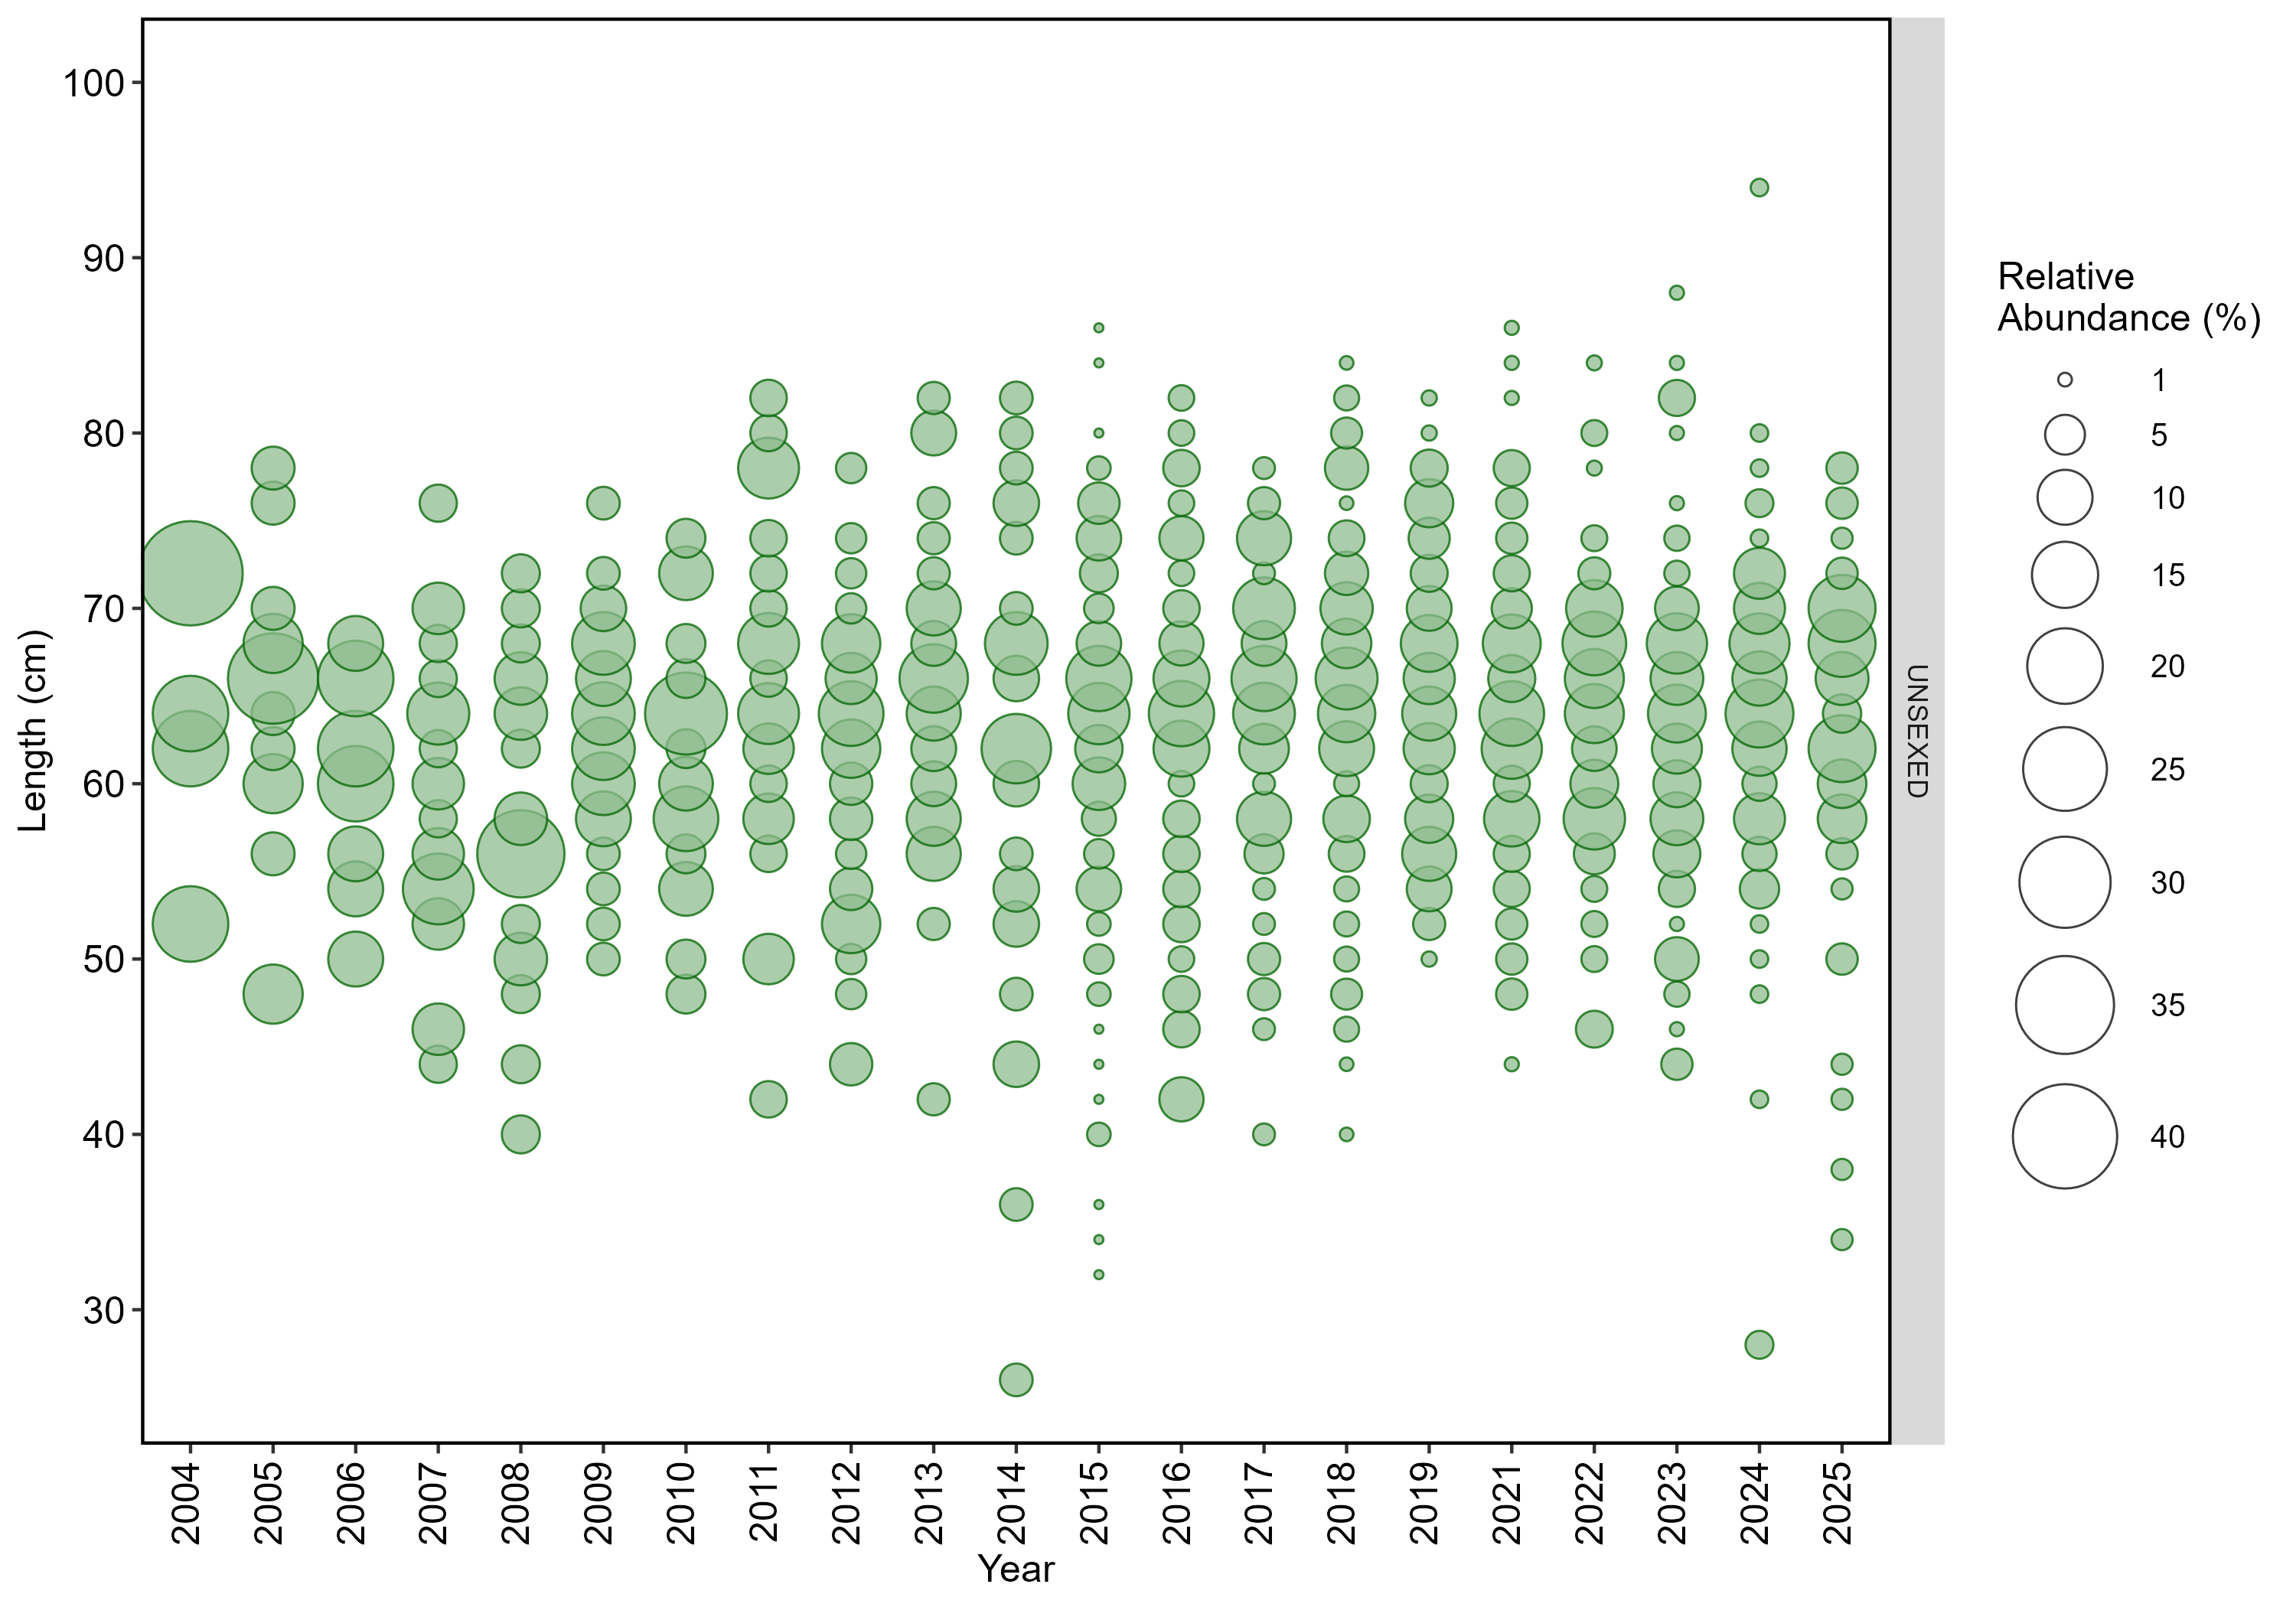
\includegraphics[width=0.95\linewidth,height=\textheight,keepaspectratio]{../plots/hkl_comps/plots/cowcod_nwfsc_hkl_length_frequency_sex_0.png}

}

\caption{Length (cm) compostion data from the NWFSC HKLS for cowcod.
Size of the circles within a year indicate higher (larger circles) and
lower (smaller circles) proportion observed by length bin.}

\end{figure}%

\newpage{}

\subsection{Darkblotched rockfish}\label{darkblotched-rockfish}

The most recent assessment of darkblotched rockfish was an update
assessment conducted in 2017. Across available data, darkblotched
rockfish have been observed and sampled by the NWFSC WCGBTS. The NWFSC
WCGBTS observed darkblotched rockfish on an average of 113 tows per
year. For this species, a total of 958 maturity samples have been
collected coastwide (regardless of stock area), with 927 read
maturities.

\begingroup\fontsize{10}{12}\selectfont
\begingroup\fontsize{10}{12}\selectfont

\begin{longtable}[t]{>{\raggedleft\arraybackslash}p{2cm}>{\raggedleft\arraybackslash}p{3.5cm}>{\raggedleft\arraybackslash}p{2cm}>{\raggedleft\arraybackslash}p{2cm}>{\raggedleft\arraybackslash}p{2cm}}
\caption{\label{tab:unnamed-chunk-176}Total number of available lengths, read ages, and unread age structures by data source and
state for darkblotched rockfish.}\\
\toprule
State & Source & Lengths & Ages & Age Structures\\
\midrule
\endfirsthead
\caption[]{Total number of available lengths, read ages, and unread age structures by data source and
state for darkblotched rockfish. (\textit{continued)}}\\
\toprule
State & Source & Lengths & Ages & Age Structures\\
\midrule
\endhead

\endfoot
\bottomrule
\endlastfoot
CA & NWFSC WCGBTS & 7,784 & 2,568 & 1,038\\
OR & NWFSC WCGBTS & 23,679 & 6,636 & 3,365\\
WA & NWFSC WCGBTS & 8,667 & 2,523 & 882\\*
\end{longtable}
\endgroup{}
\endgroup{}

\begin{figure}[H]

{\centering 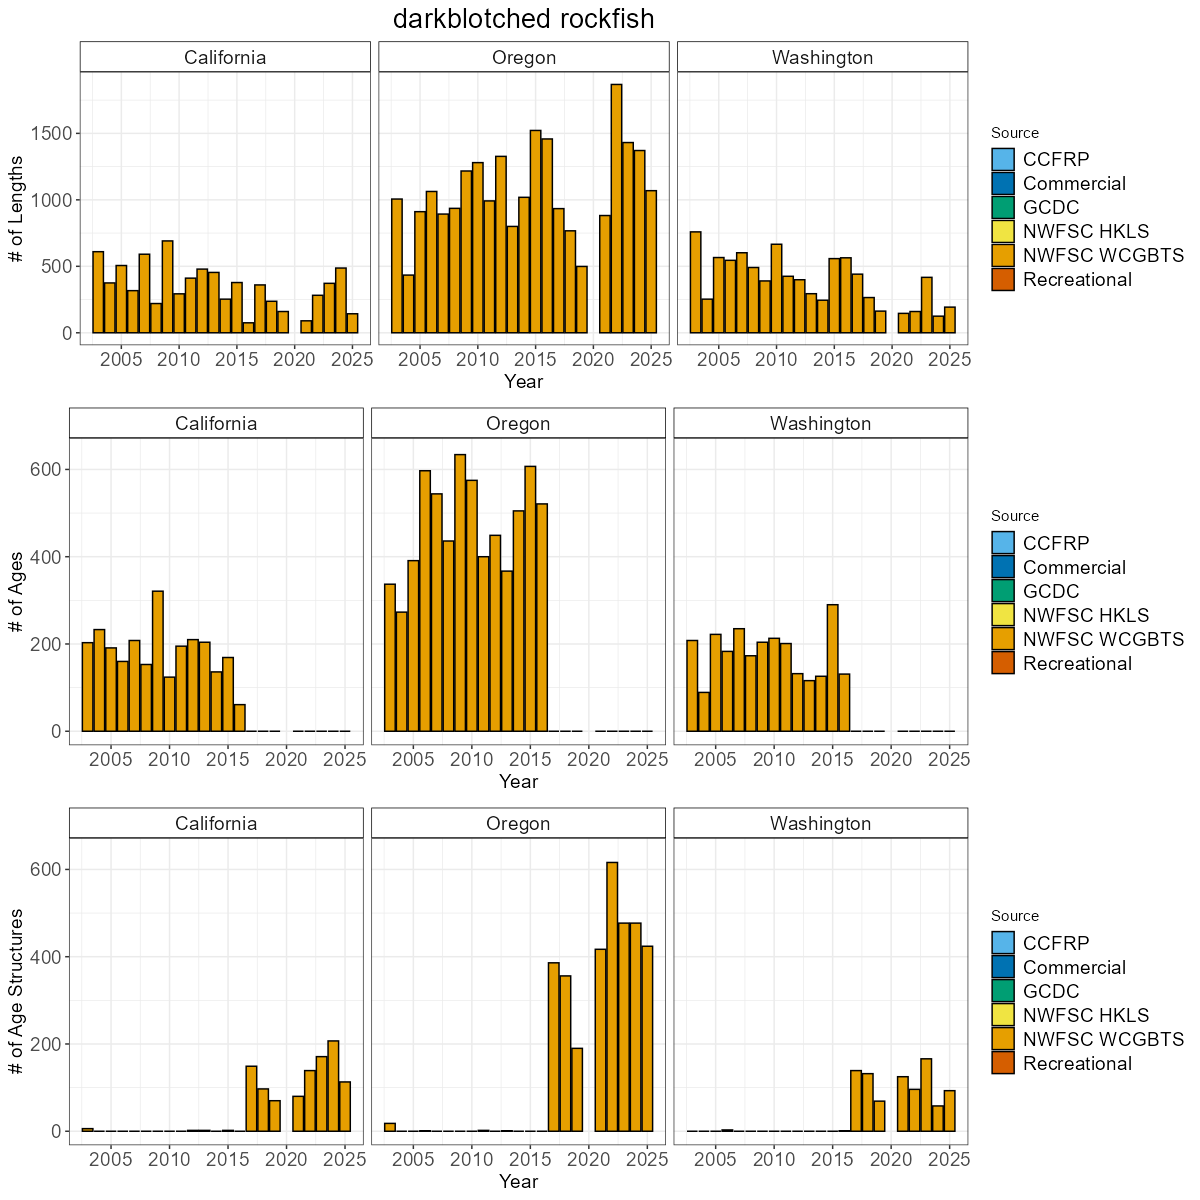
\includegraphics[width=0.95\linewidth,height=\textheight,keepaspectratio]{../plots/state_comparisons/darkblotched_rockfish_state_compositions.png}

}

\caption{Total number of available lengths, read ages, and unread age
structures by data source by year for darkblotched rockfish. Note the
y-axis maximum may differ by data type.}

\end{figure}%

\begin{figure}[H]

{\centering 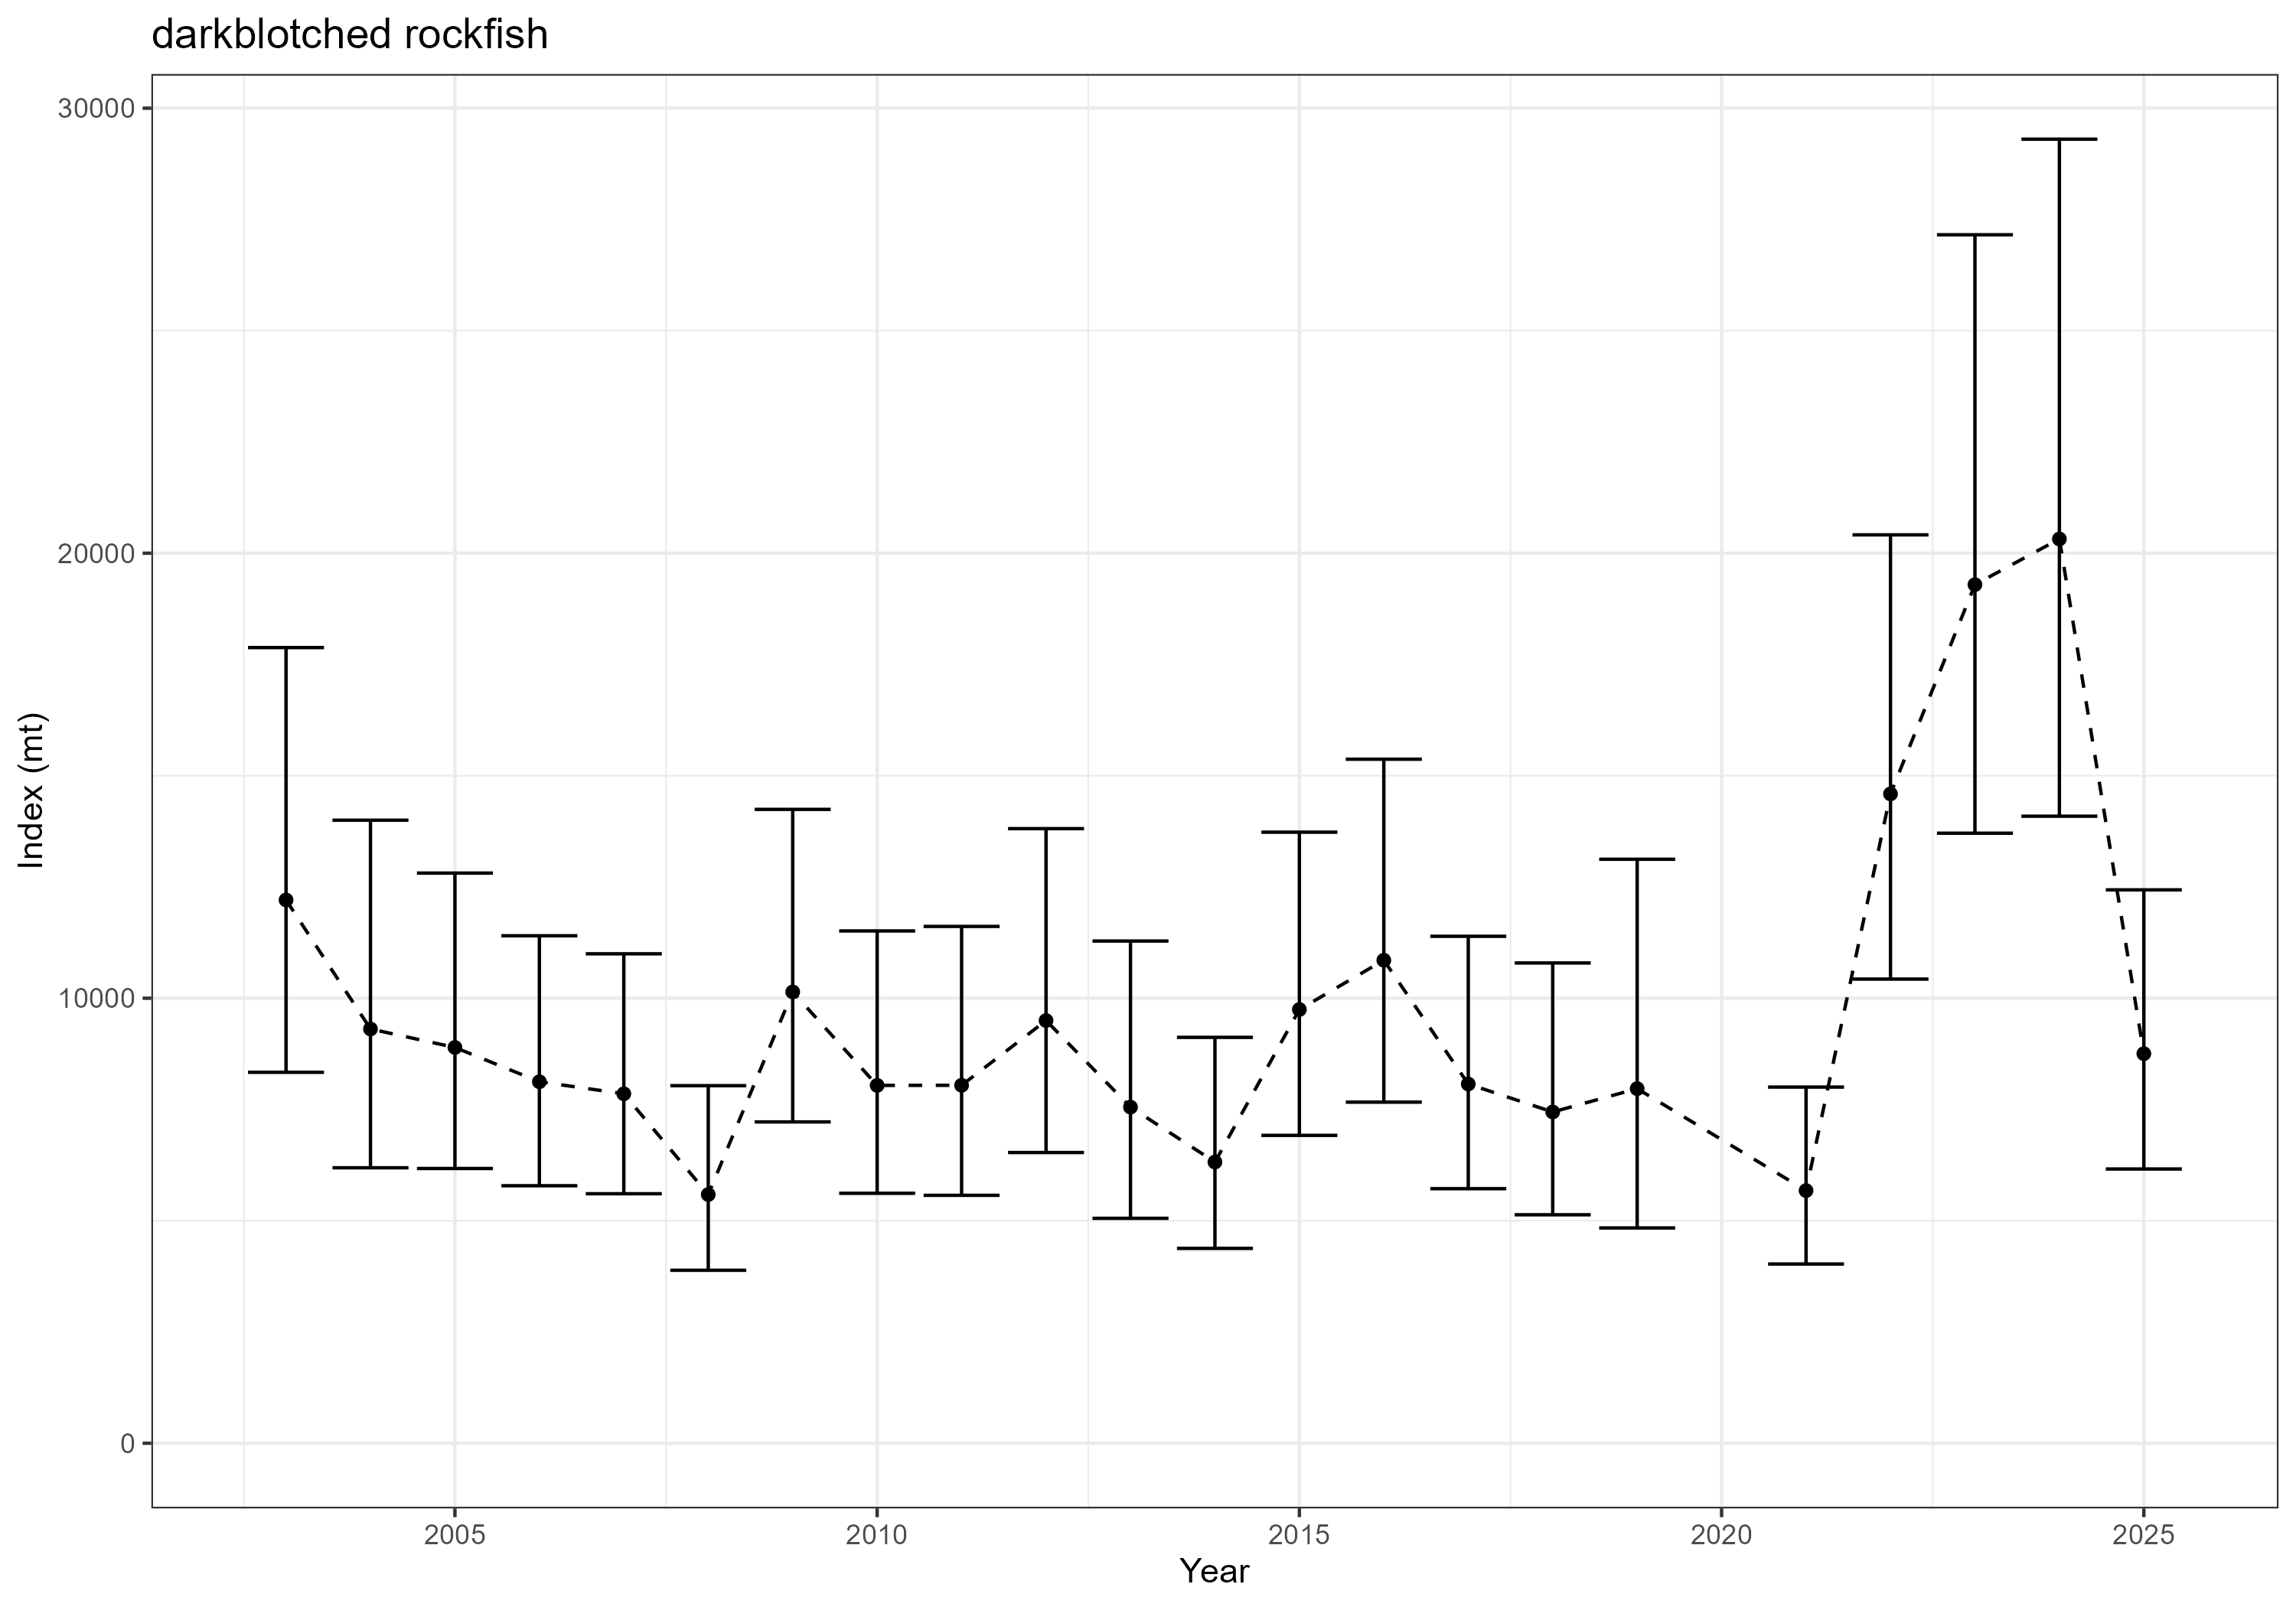
\includegraphics[width=0.95\linewidth,height=\textheight,keepaspectratio]{../plots/wcgbts_indices/darkblotched_rockfish_index.png}

}

\caption{Estimated relative index of abundance for darkblotched rockfish
from the NWFSC WCGBTS.}

\end{figure}%

\begin{figure}[H]

{\centering 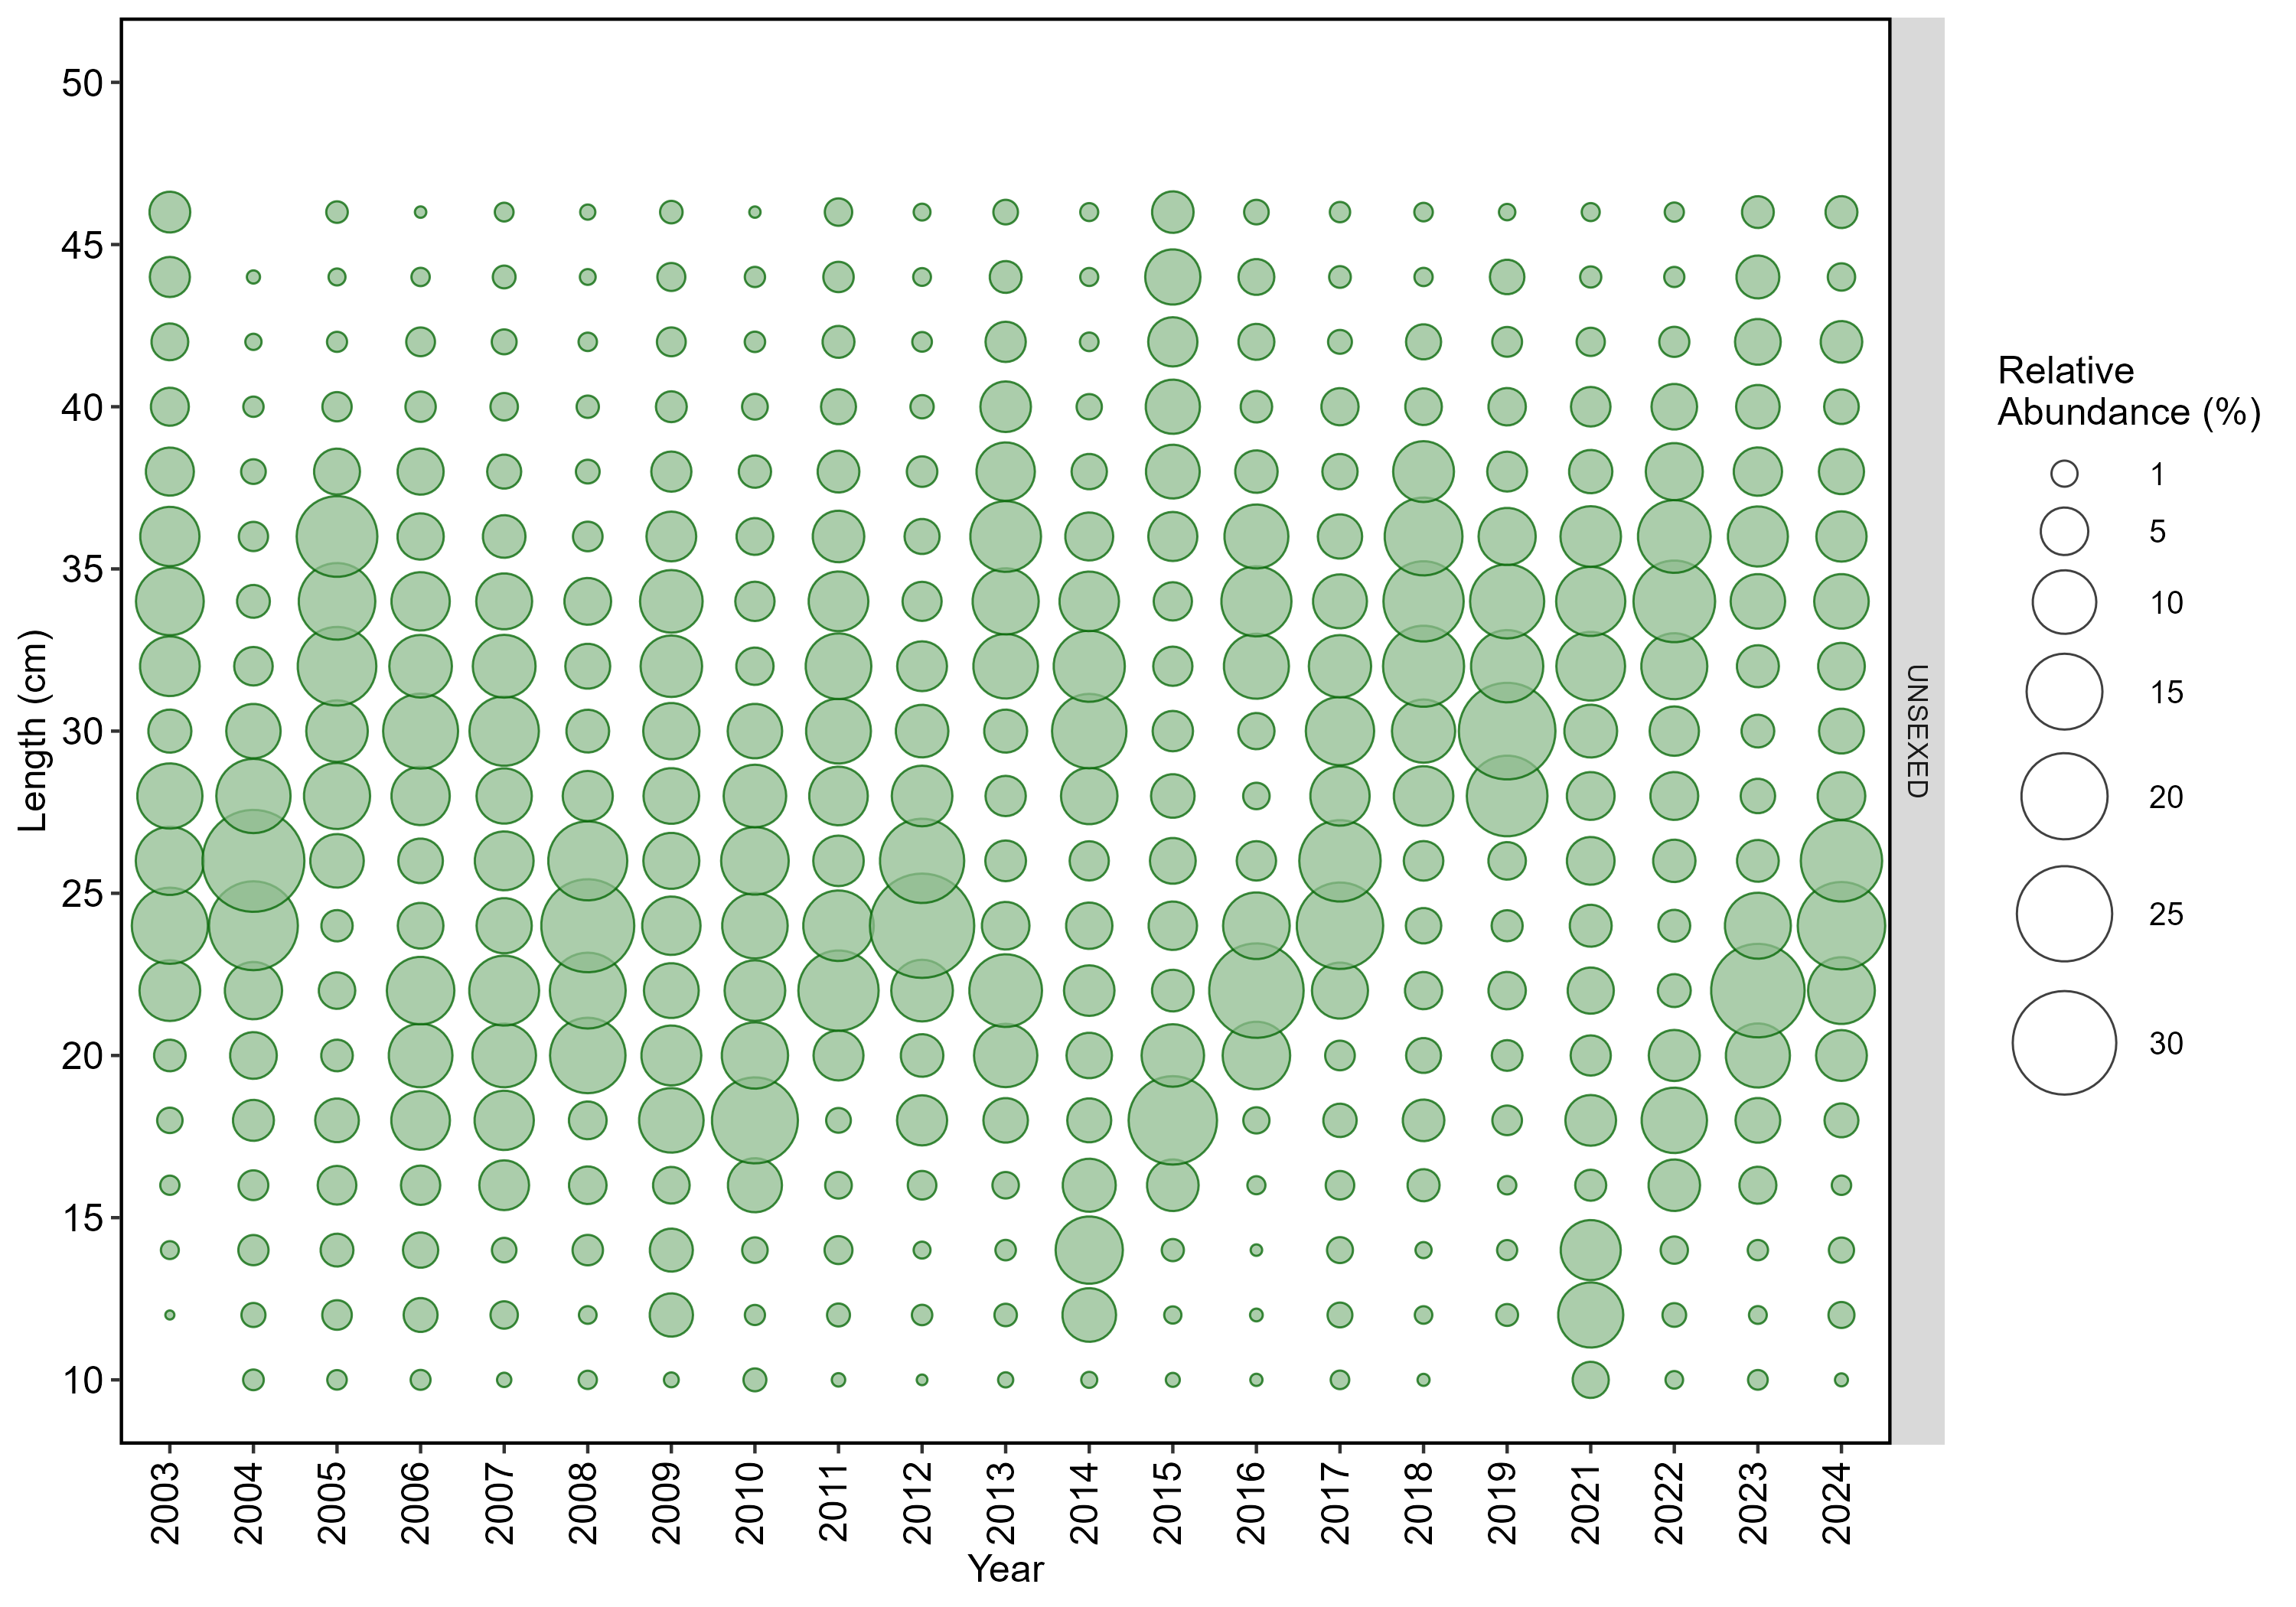
\includegraphics[width=0.95\linewidth,height=\textheight,keepaspectratio]{../plots/wcgbts_comps/plots/darkblotched rockfish_length_frequency_sex_0.png}

}

\caption{Length (cm) compostion data from the NWFSC WCGBTS for
darkblotched rockfish. Size of the circles within a year indicate higher
(larger circles) and lower (smaller circles) proportion observed by
length bin.}

\end{figure}%

\newpage{}

\subsection{Dover sole}\label{dover-sole}

The most recent assessment of Dover sole was a benchmark assessment
conducted in 2021. Across available data, Dover sole have been observed
and sampled by the NWFSC WCGBTS. The NWFSC WCGBTS observed Dover sole on
an average of 536 tows per year. For this species, a total of 820
maturity samples have been collected coastwide (regardless of stock
area), with 635 read maturities.

\begingroup\fontsize{10}{12}\selectfont
\begingroup\fontsize{10}{12}\selectfont

\begin{longtable}[t]{>{\raggedleft\arraybackslash}p{2cm}>{\raggedleft\arraybackslash}p{3.5cm}>{\raggedleft\arraybackslash}p{2cm}>{\raggedleft\arraybackslash}p{2cm}>{\raggedleft\arraybackslash}p{2cm}}
\caption{\label{tab:unnamed-chunk-193}Total number of available lengths, read ages, and unread age structures by data source and
state for Dover sole.}\\
\toprule
State & Source & Lengths & Ages & Age Structures\\
\midrule
\endfirsthead
\caption[]{Total number of available lengths, read ages, and unread age structures by data source and
state for Dover sole. (\textit{continued)}}\\
\toprule
State & Source & Lengths & Ages & Age Structures\\
\midrule
\endhead

\endfoot
\bottomrule
\endlastfoot
CA & NWFSC WCGBTS & 89,094 & 8,707 & 6,406\\
OR & NWFSC WCGBTS & 71,164 & 5,836 & 4,531\\
WA & NWFSC WCGBTS & 33,050 & 2,581 & 2,145\\*
\end{longtable}
\endgroup{}
\endgroup{}

\begin{figure}[H]

{\centering 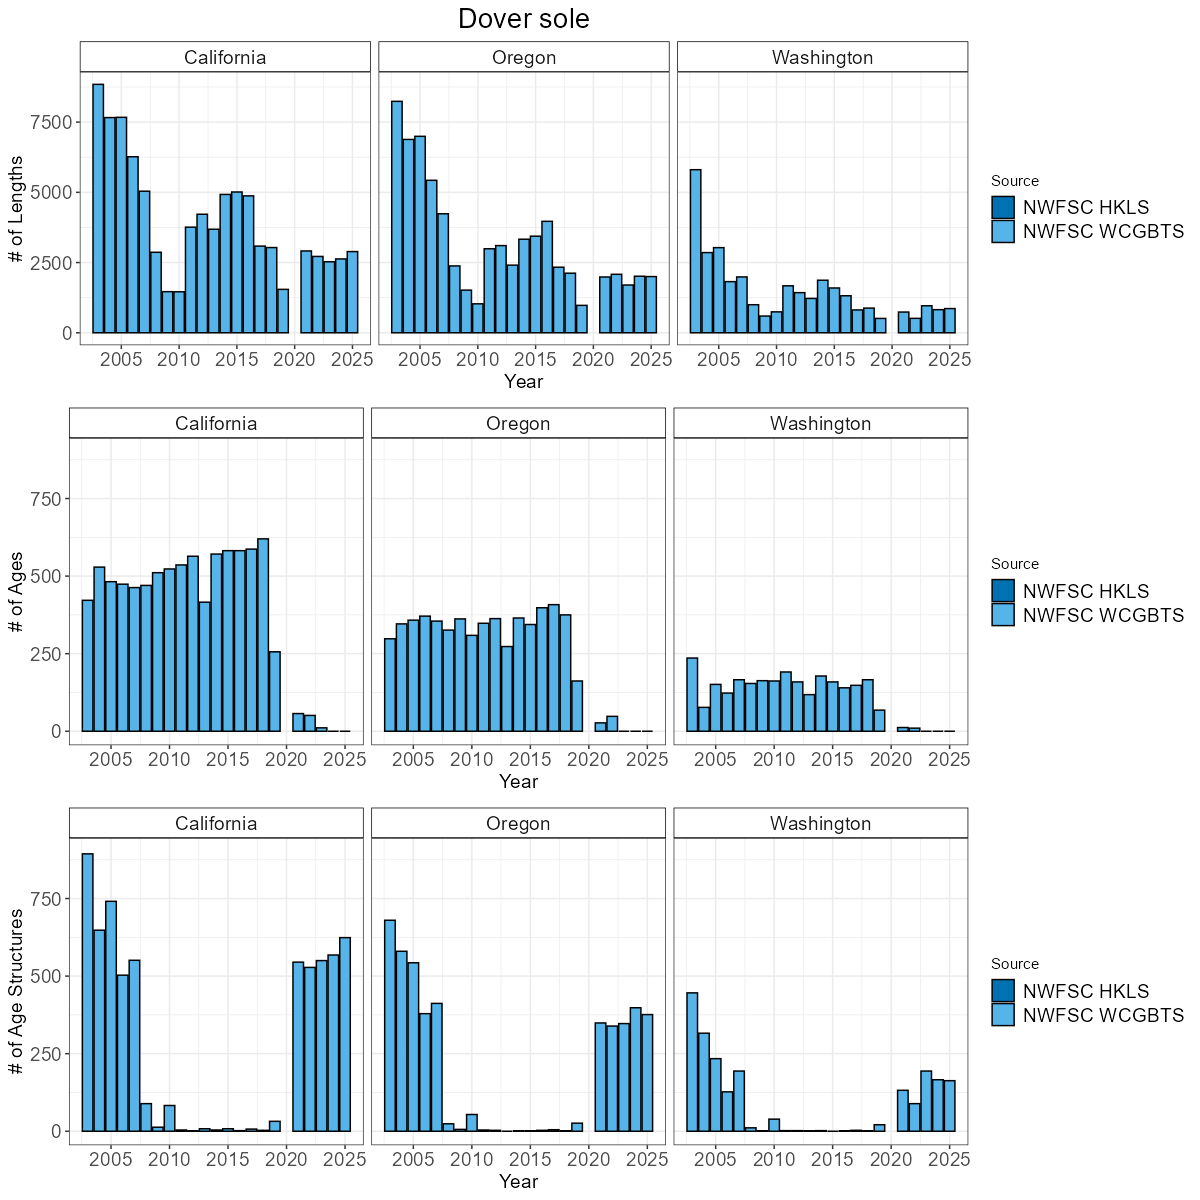
\includegraphics[width=0.95\linewidth,height=\textheight,keepaspectratio]{../plots/state_comparisons/dover_sole_state_compositions.png}

}

\caption{Total number of available lengths, read ages, and unread age
structures by data source by year for Dover sole. Note the y-axis
maximum may differ by data type.}

\end{figure}%

\begin{figure}[H]

{\centering 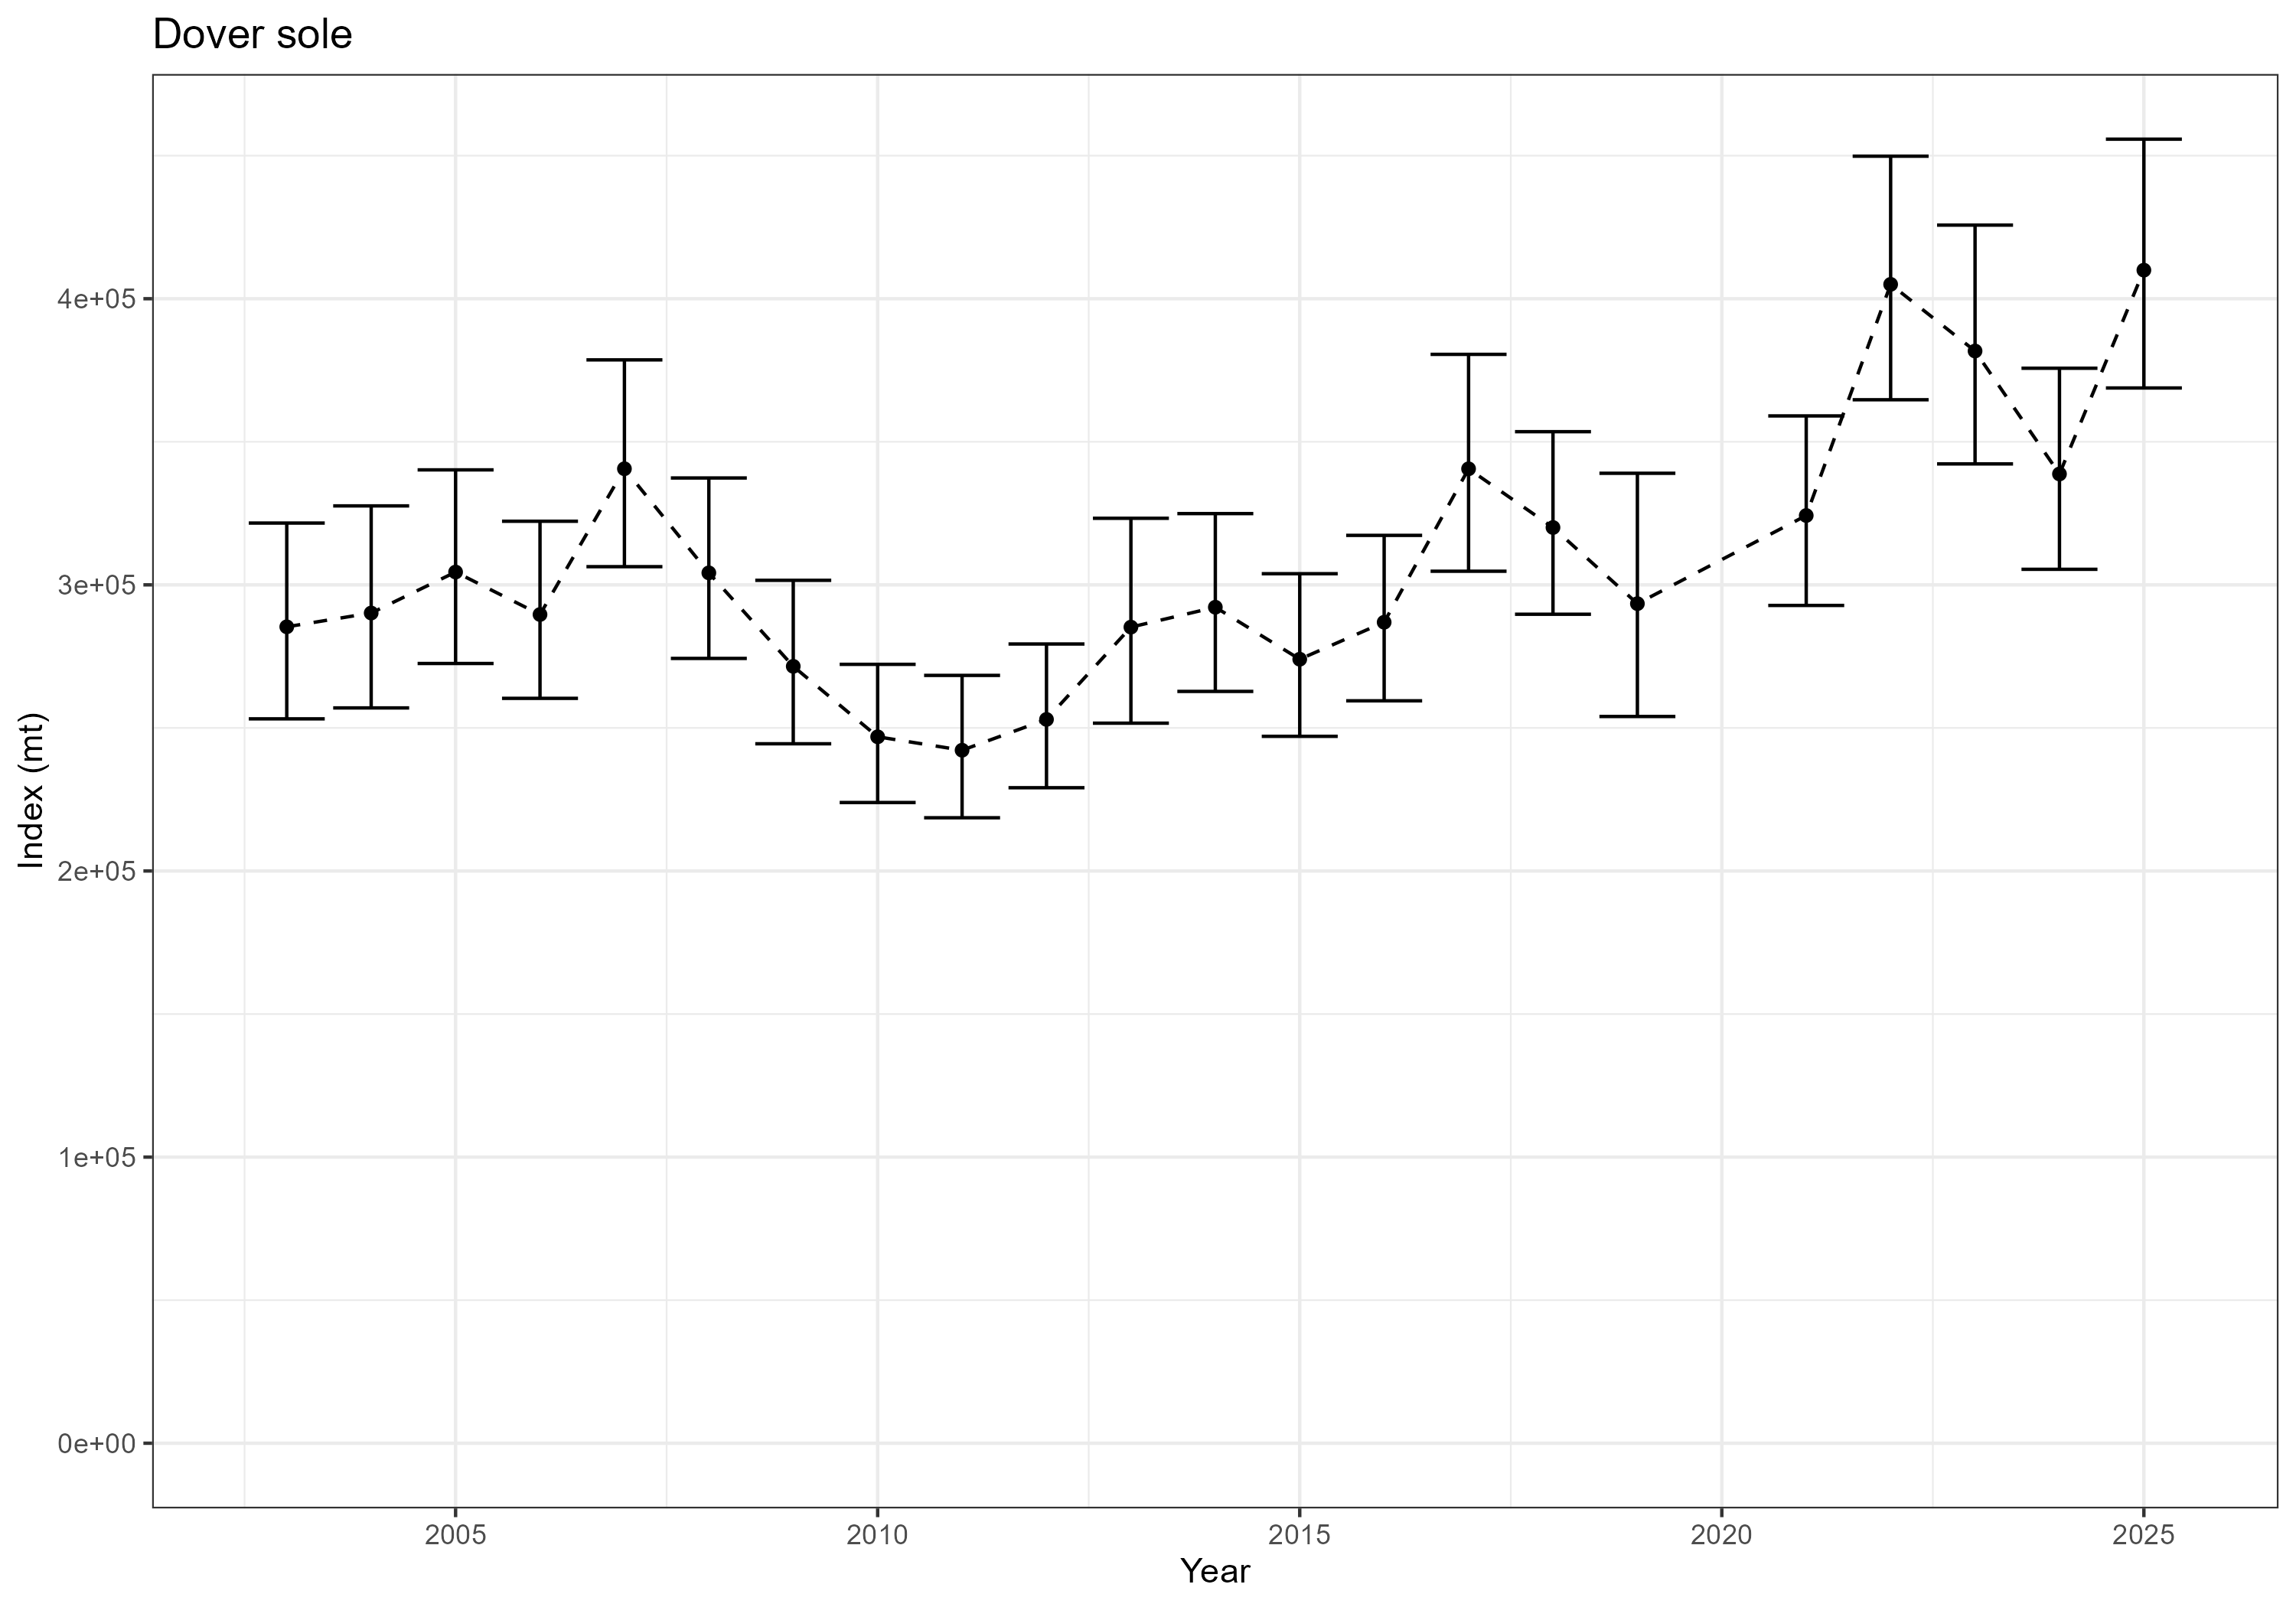
\includegraphics[width=0.95\linewidth,height=\textheight,keepaspectratio]{../plots/wcgbts_indices/dover_sole_index.png}

}

\caption{Estimated relative index of abundance for Dover sole from the
NWFSC WCGBTS.}

\end{figure}%

\begin{figure}[H]

{\centering 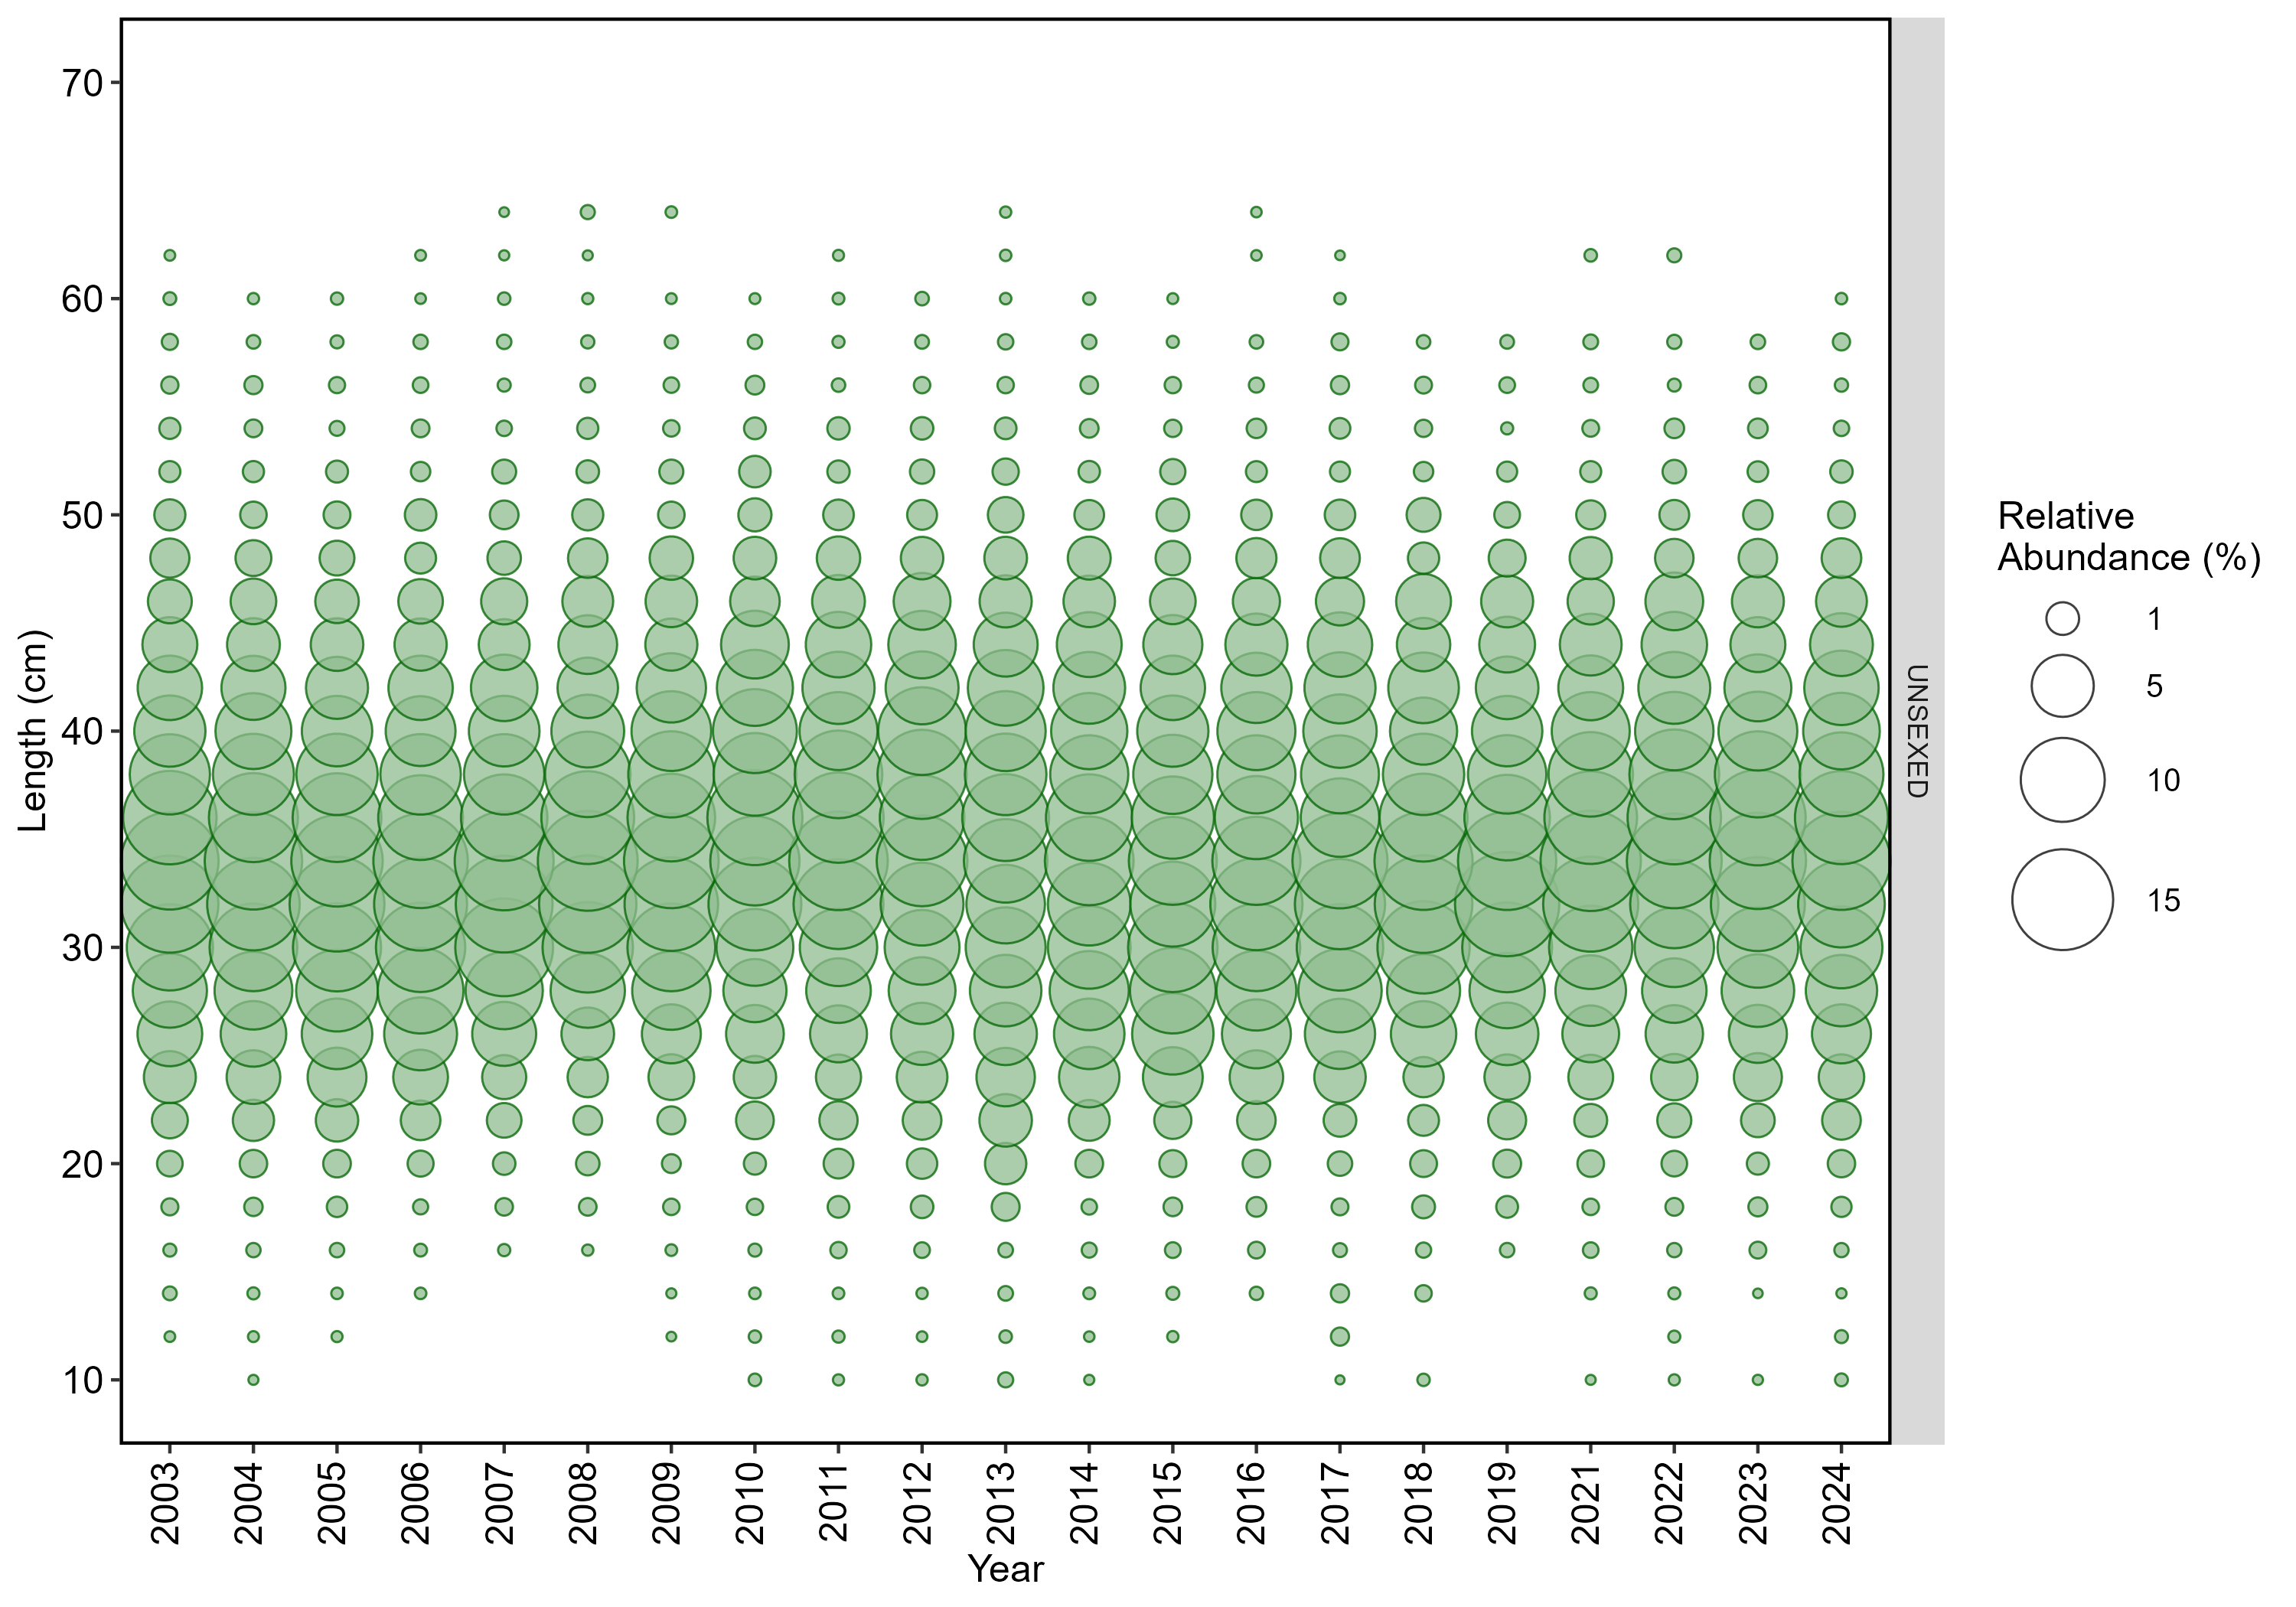
\includegraphics[width=0.95\linewidth,height=\textheight,keepaspectratio]{../plots/wcgbts_comps/plots/Dover sole_length_frequency_sex_0.png}

}

\caption{Length (cm) compostion data from the NWFSC WCGBTS for Dover
sole. Size of the circles within a year indicate higher (larger circles)
and lower (smaller circles) proportion observed by length bin.}

\end{figure}%

\newpage{}

\subsection{English sole}\label{english-sole}

The most recent assessment of English sole was a data-moderate
assessment conducted in 2013. Across available data, English sole have
been observed and sampled by the NWFSC WCGBTS. The NWFSC WCGBTS observed
English sole on an average of 266 tows per year. For this species, a
total of 174 maturity samples have been collected coastwide (regardless
of stock area), with 0 read maturities.

\begingroup\fontsize{10}{12}\selectfont
\begingroup\fontsize{10}{12}\selectfont

\begin{longtable}[t]{>{\raggedleft\arraybackslash}p{2cm}>{\raggedleft\arraybackslash}p{3.5cm}>{\raggedleft\arraybackslash}p{2cm}>{\raggedleft\arraybackslash}p{2cm}>{\raggedleft\arraybackslash}p{2cm}}
\caption{\label{tab:unnamed-chunk-210}Total number of available lengths, read ages, and unread age structures by data source and
state for English sole.}\\
\toprule
State & Source & Lengths & Ages & Age Structures\\
\midrule
\endfirsthead
\caption[]{Total number of available lengths, read ages, and unread age structures by data source and
state for English sole. (\textit{continued)}}\\
\toprule
State & Source & Lengths & Ages & Age Structures\\
\midrule
\endhead

\endfoot
\bottomrule
\endlastfoot
CA & NWFSC WCGBTS & 46,065 & 478 & 9,110\\
OR & NWFSC WCGBTS & 31,844 & 279 & 5,503\\
WA & NWFSC WCGBTS & 14,163 & 141 & 3,021\\*
\end{longtable}
\endgroup{}
\endgroup{}

\begin{figure}[H]

{\centering 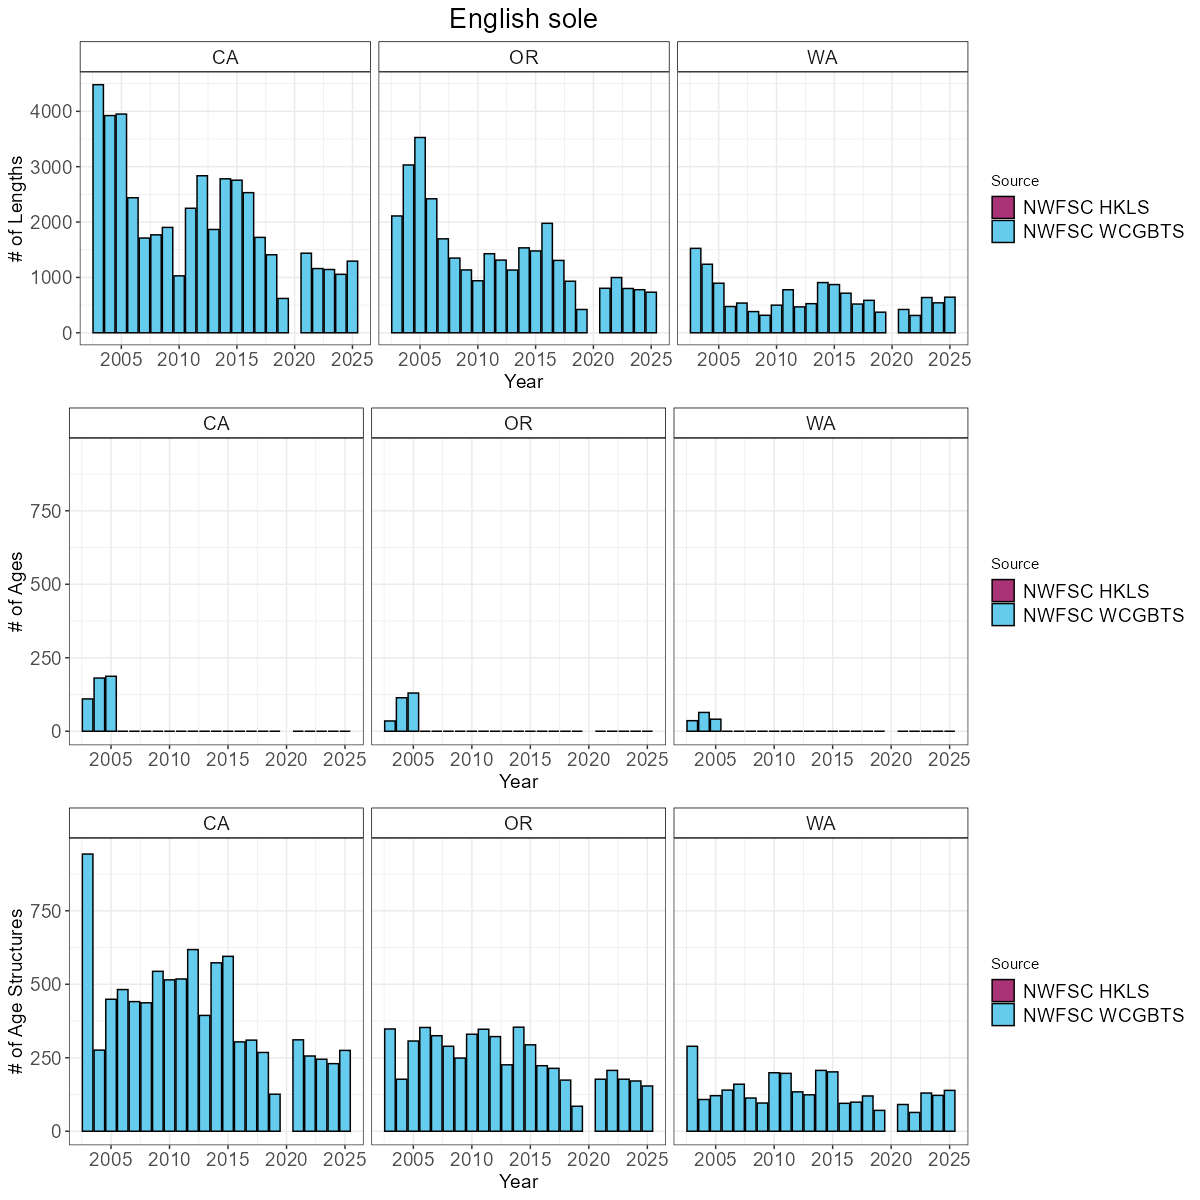
\includegraphics[width=0.95\linewidth,height=\textheight,keepaspectratio]{../plots/state_comparisons/english_sole_state_compositions.png}

}

\caption{Total number of available lengths, read ages, and unread age
structures by data source by year for English sole. Note the y-axis
maximum may differ by data type.}

\end{figure}%

\begin{figure}[H]

{\centering 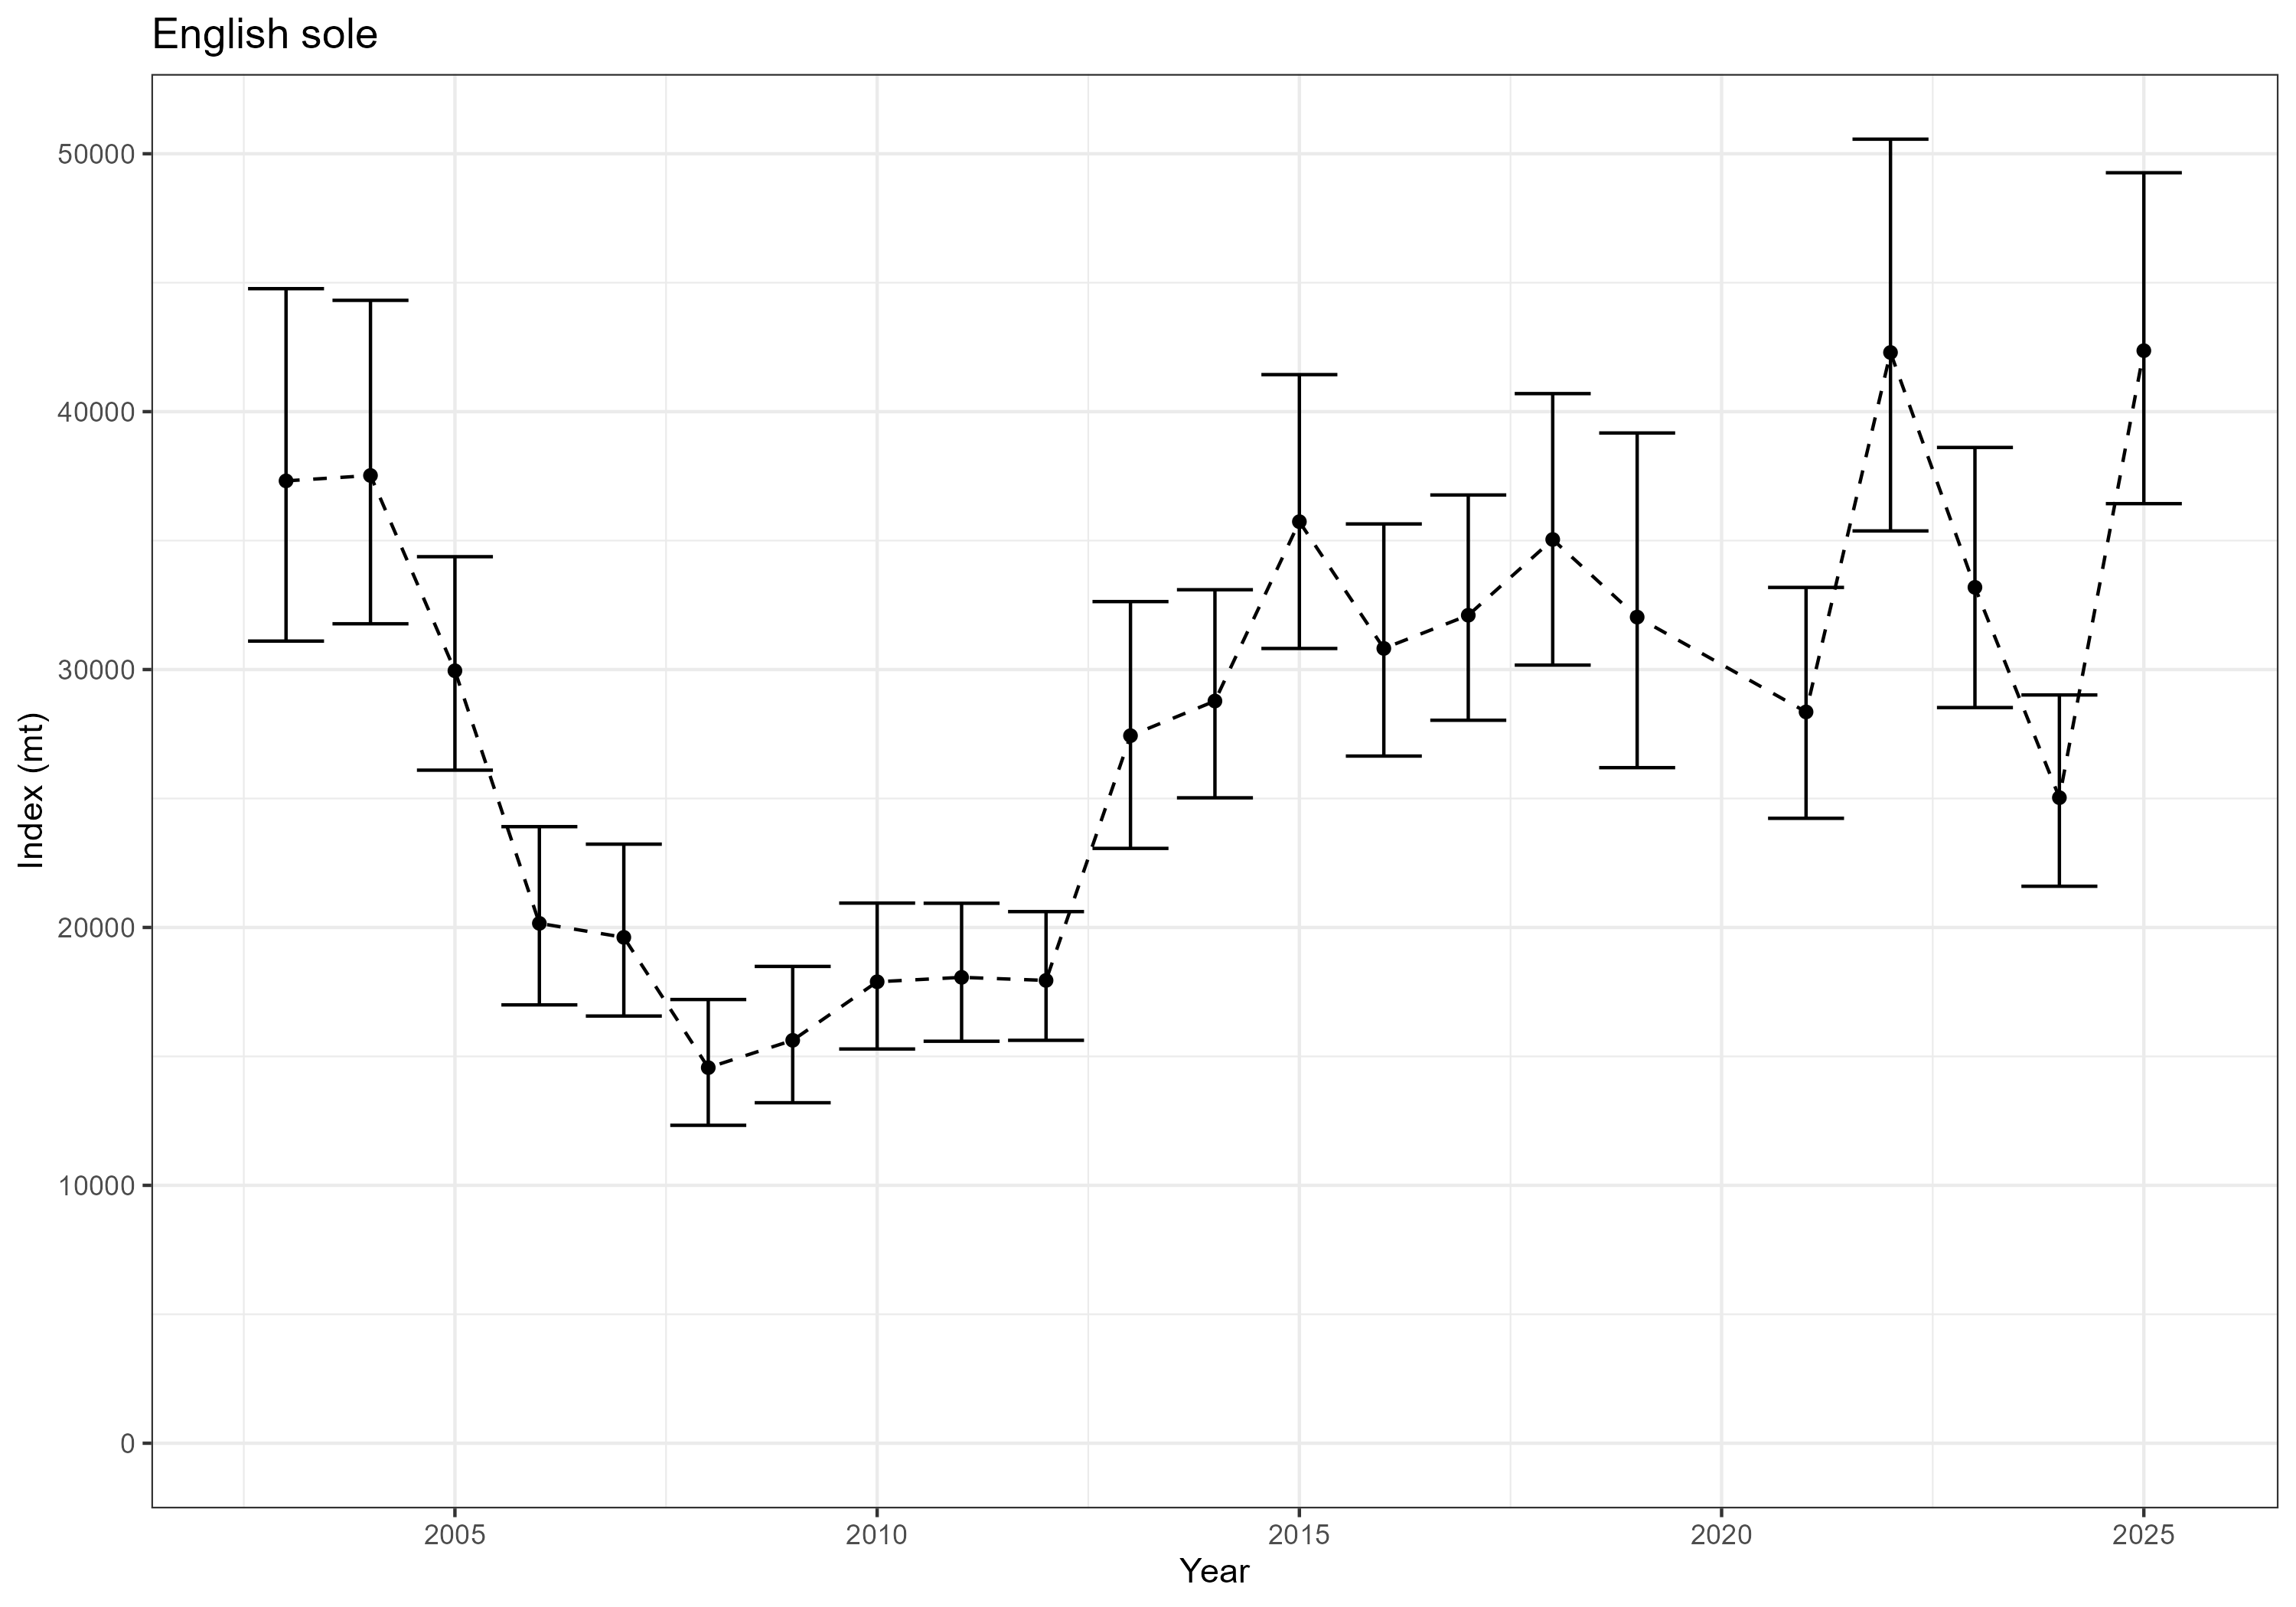
\includegraphics[width=0.95\linewidth,height=\textheight,keepaspectratio]{../plots/wcgbts_indices/english_sole_index.png}

}

\caption{Estimated relative index of abundance for English sole from the
NWFSC WCGBTS.}

\end{figure}%

\begin{figure}[H]

{\centering 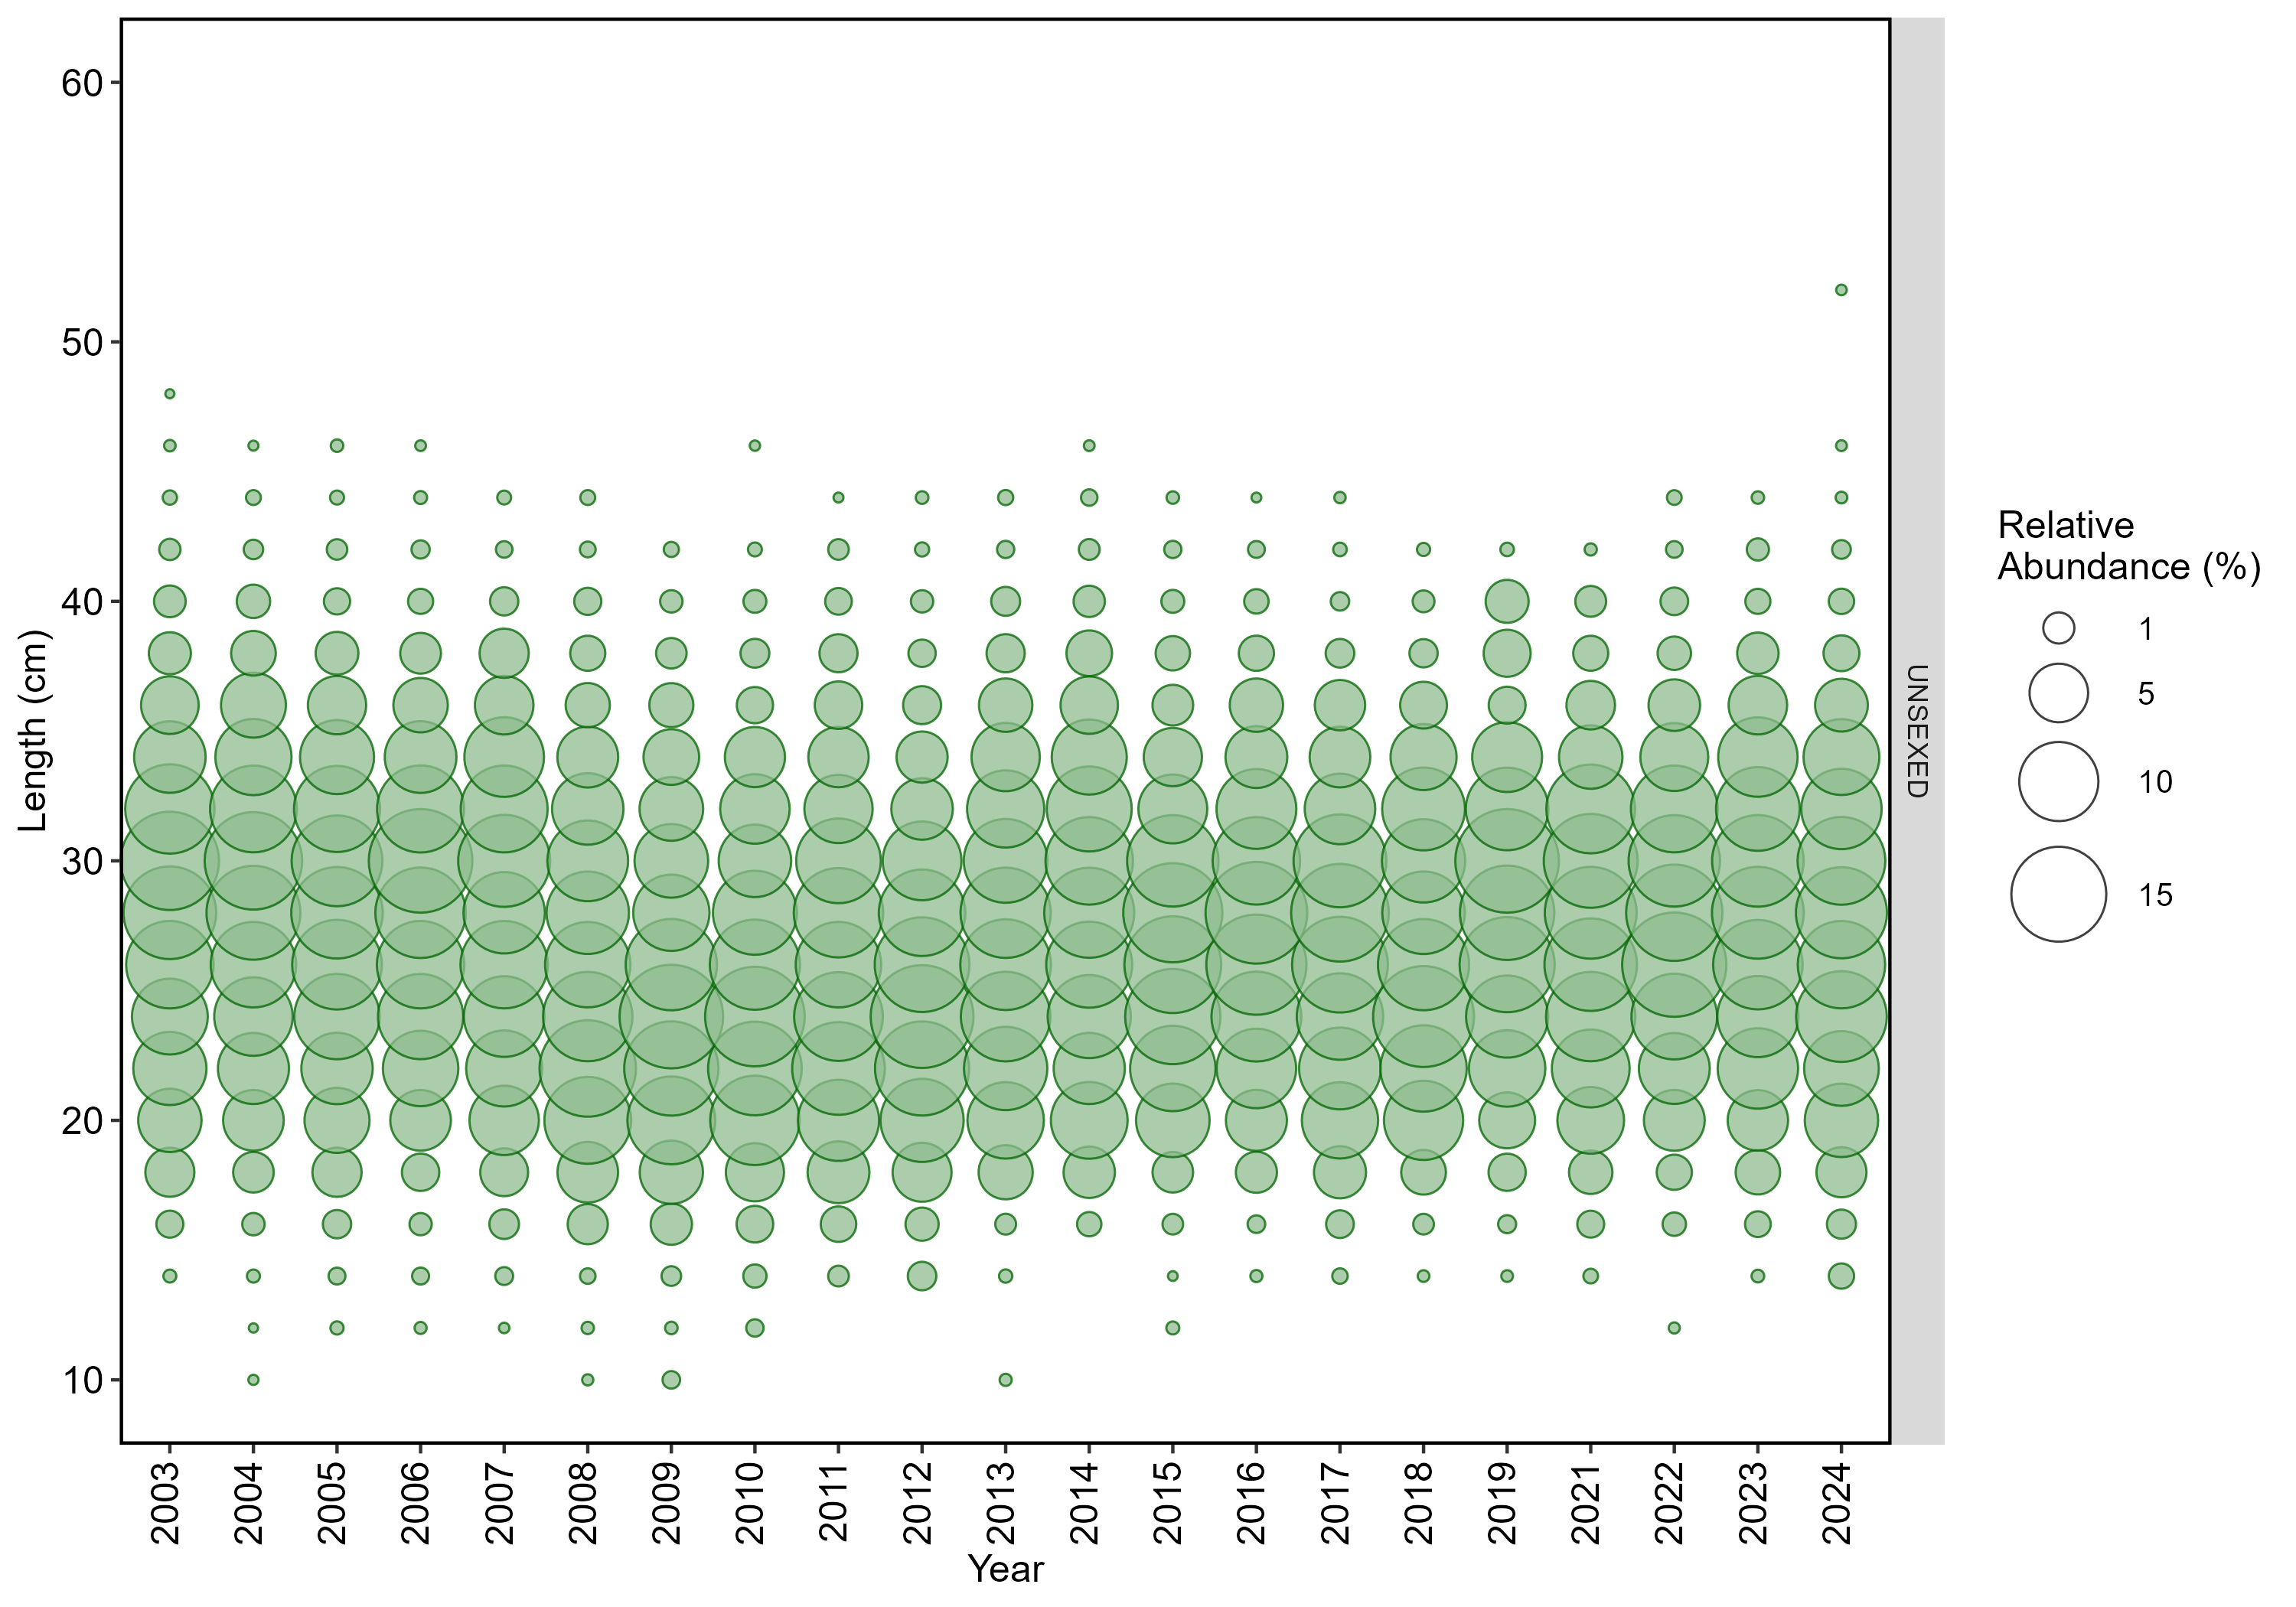
\includegraphics[width=0.95\linewidth,height=\textheight,keepaspectratio]{../plots/wcgbts_comps/plots/English sole_length_frequency_sex_0.png}

}

\caption{Length (cm) compostion data from the NWFSC WCGBTS for English
sole. Size of the circles within a year indicate higher (larger circles)
and lower (smaller circles) proportion observed by length bin.}

\end{figure}%

\newpage{}

\subsection{Flathead sole}\label{flathead-sole}

To date, no assessment or analysis has been conducted on flathead sole.
Across available data, flathead sole have been observed and sampled by
the NWFSC WCGBTS. The NWFSC WCGBTS observed flathead sole on an average
of 52 tows per year. For this species, a total of 0 maturity samples
have been collected coastwide (regardless of stock area).

\begingroup\fontsize{10}{12}\selectfont
\begingroup\fontsize{10}{12}\selectfont

\begin{longtable}[t]{>{\raggedleft\arraybackslash}p{2cm}>{\raggedleft\arraybackslash}p{3.5cm}>{\raggedleft\arraybackslash}p{2cm}>{\raggedleft\arraybackslash}p{2cm}>{\raggedleft\arraybackslash}p{2cm}}
\caption{\label{tab:unnamed-chunk-227}Total number of available lengths, read ages, and unread age structures by data source and
state for flathead sole.}\\
\toprule
State & Source & Lengths & Ages & Age Structures\\
\midrule
\endfirsthead
\caption[]{Total number of available lengths, read ages, and unread age structures by data source and
state for flathead sole. (\textit{continued)}}\\
\toprule
State & Source & Lengths & Ages & Age Structures\\
\midrule
\endhead

\endfoot
\bottomrule
\endlastfoot
CA & NWFSC WCGBTS & 77 & 0 & 39\\
OR & NWFSC WCGBTS & 4,985 & 0 & 2,154\\
WA & NWFSC WCGBTS & 7,345 & 0 & 1,732\\*
\end{longtable}
\endgroup{}
\endgroup{}

\begin{figure}[H]

{\centering 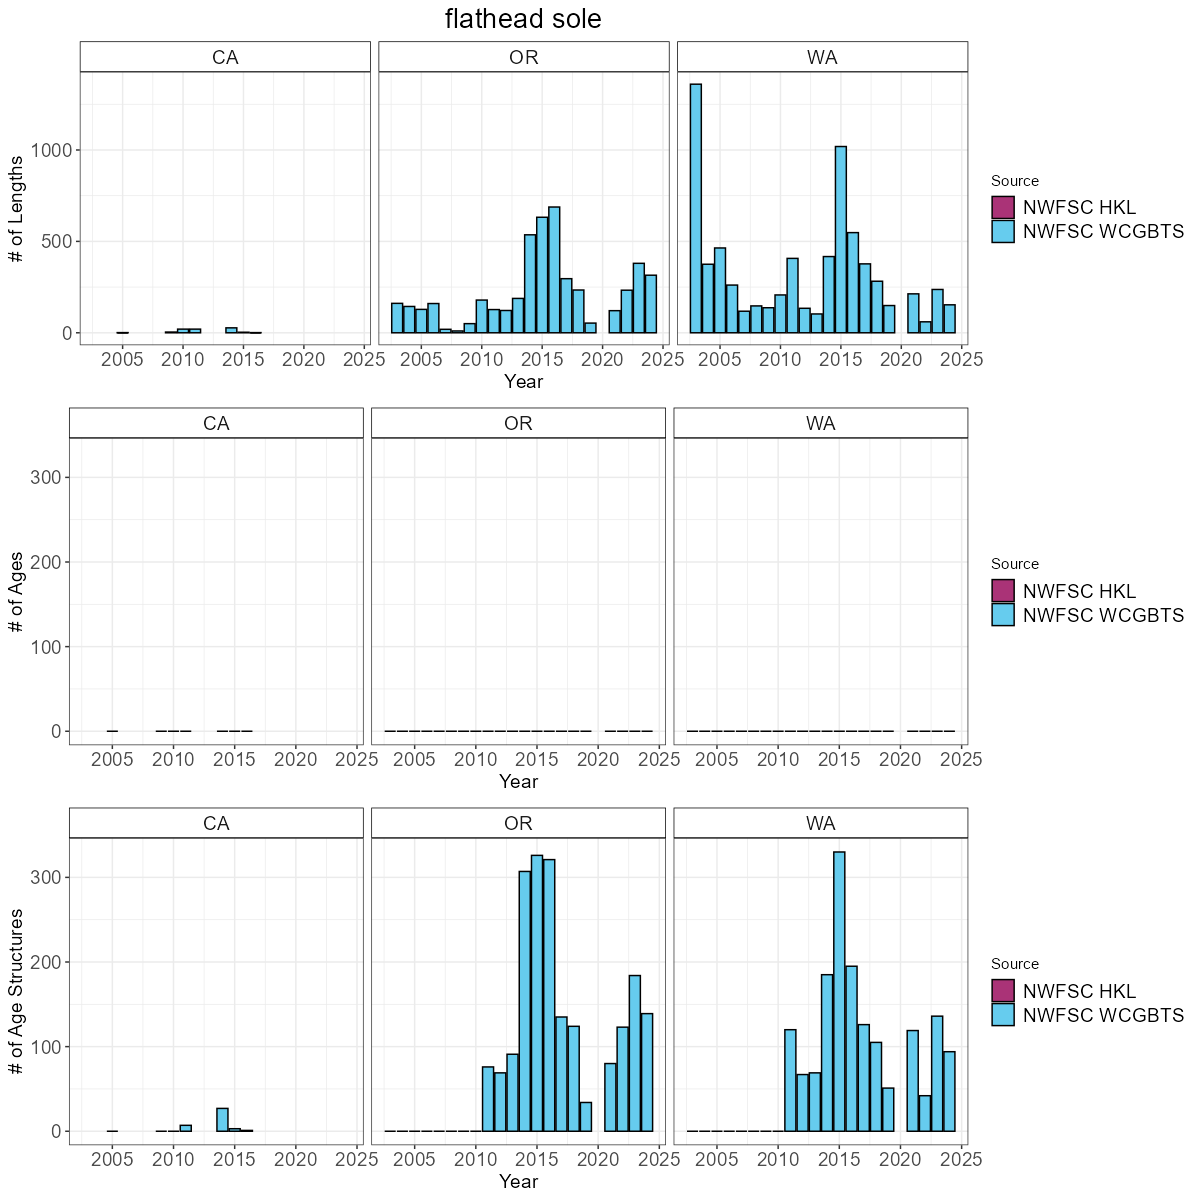
\includegraphics[width=0.95\linewidth,height=\textheight,keepaspectratio]{../plots/state_comparisons/flathead_sole_state_compositions.png}

}

\caption{Total number of available lengths, read ages, and unread age
structures by data source by year for flathead sole. Note the y-axis
maximum may differ by data type.}

\end{figure}%

\begin{figure}[H]

{\centering 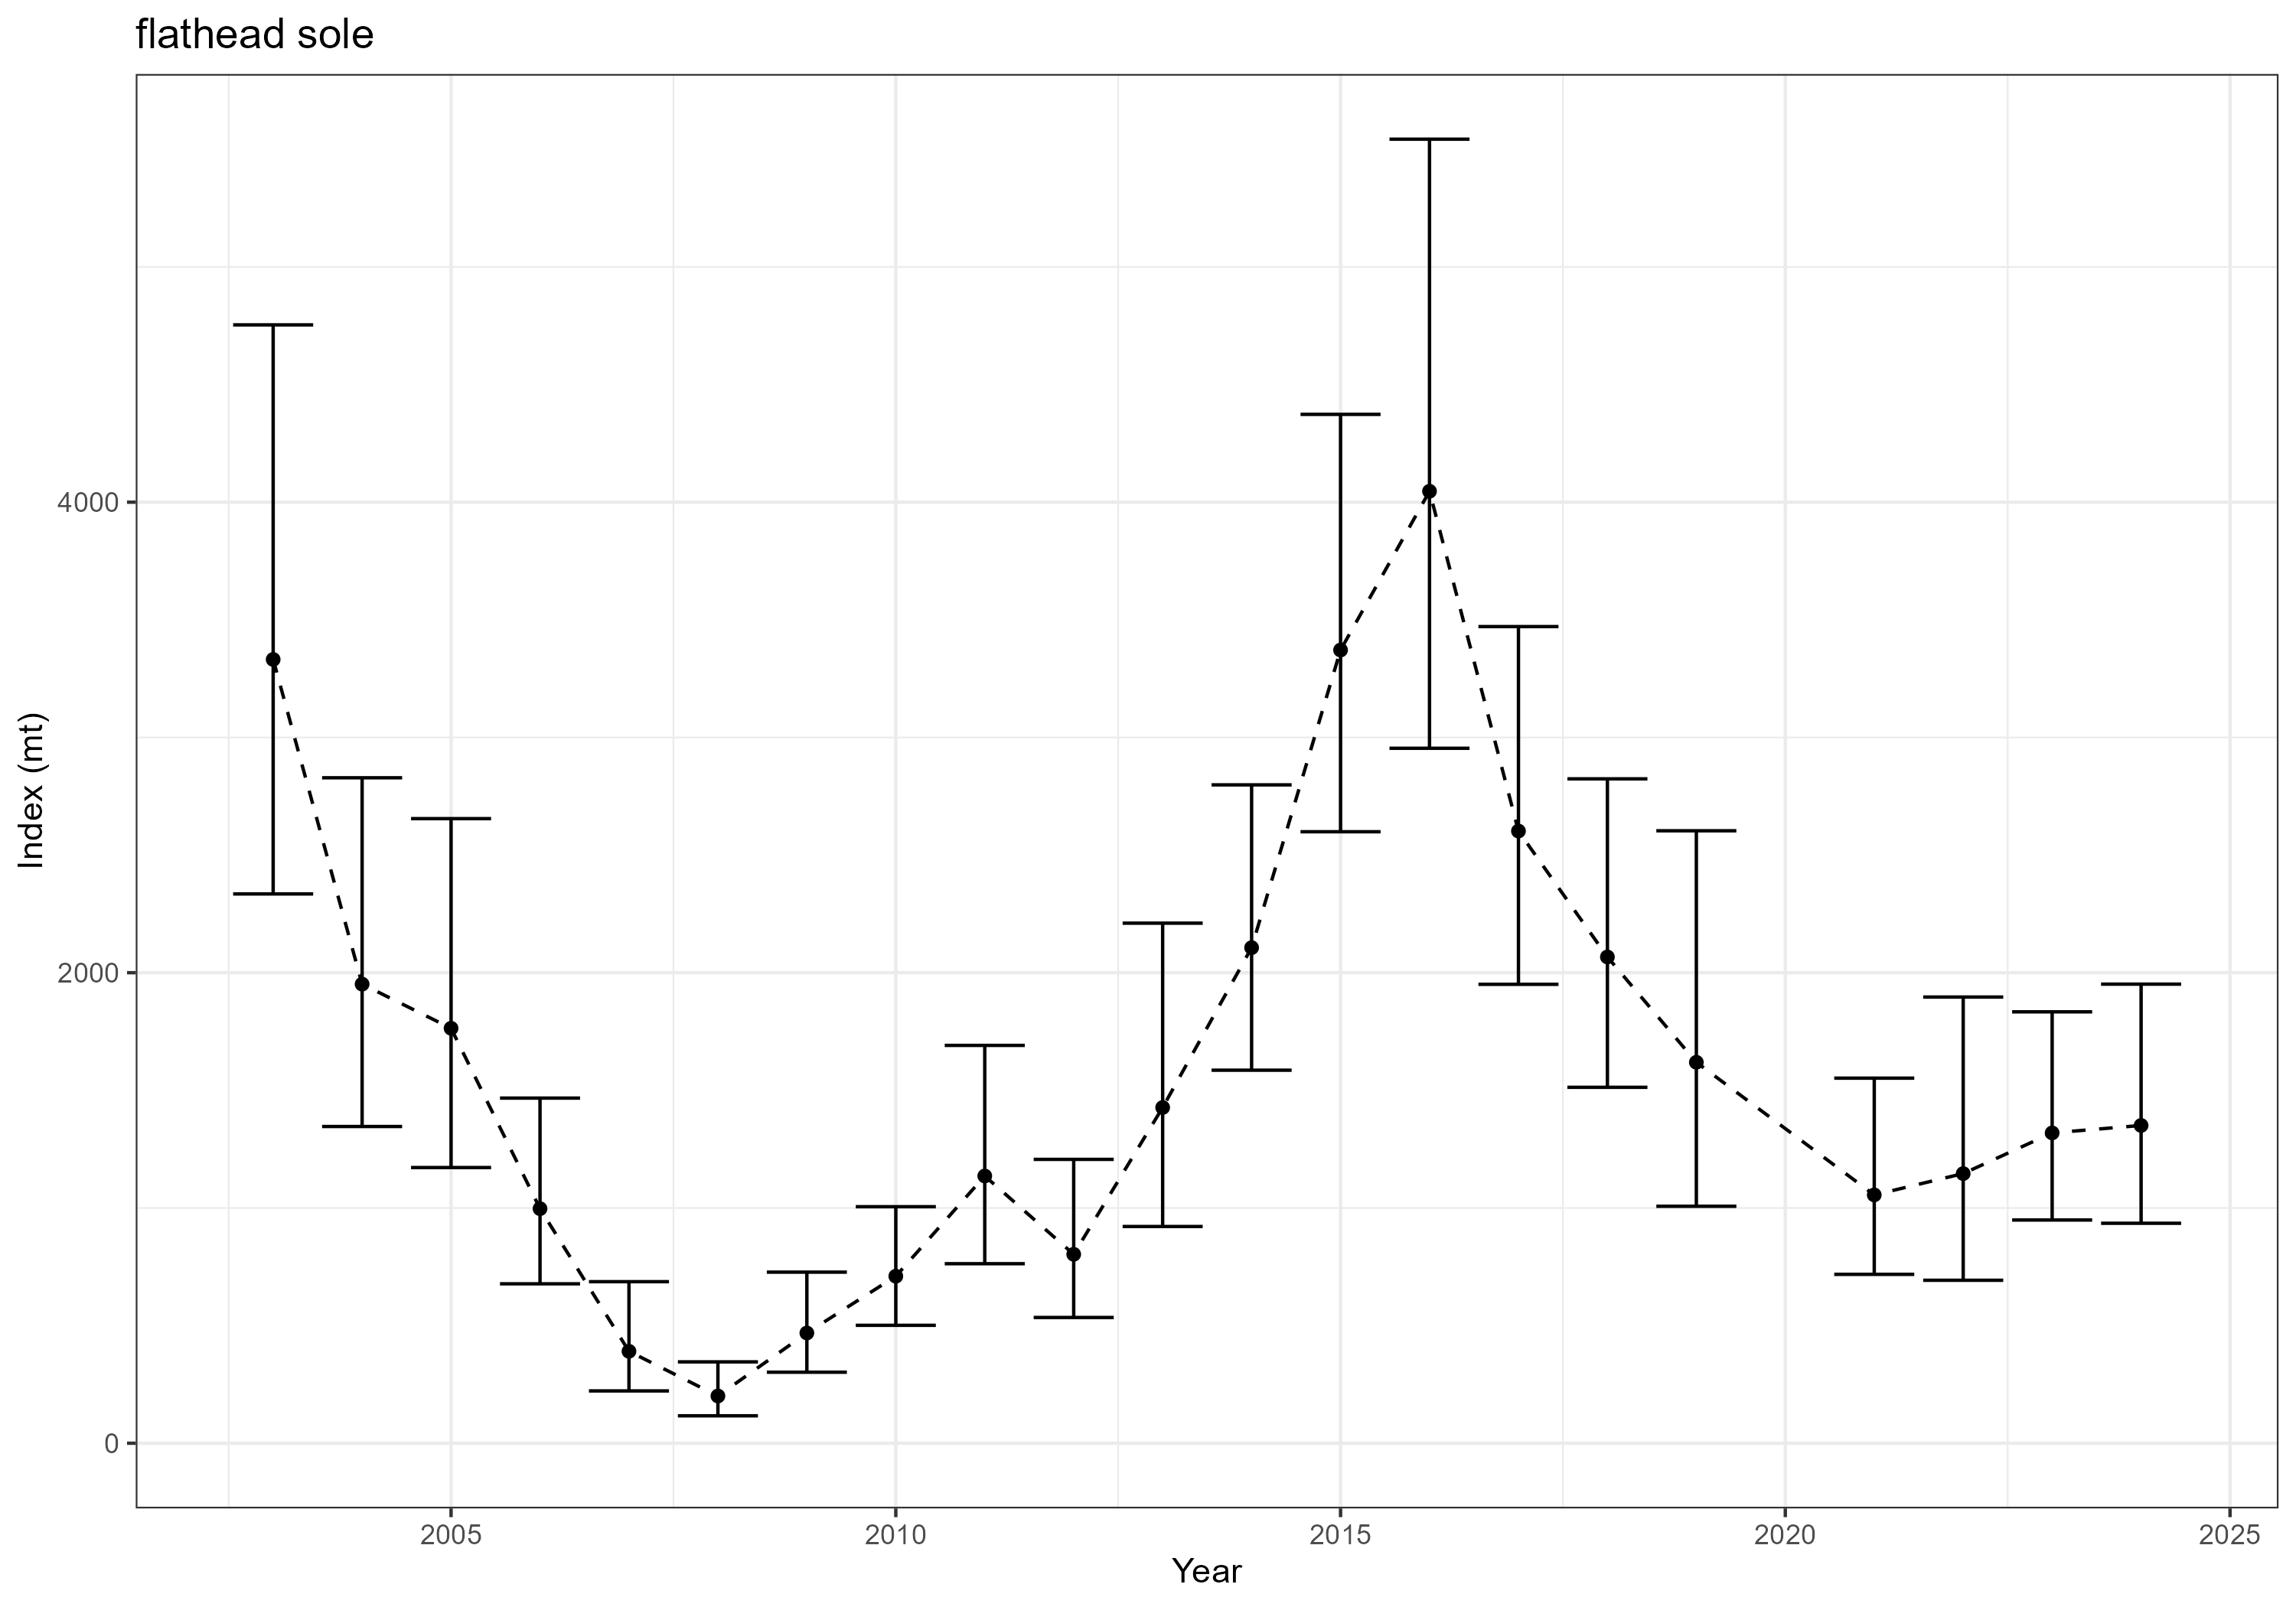
\includegraphics[width=0.95\linewidth,height=\textheight,keepaspectratio]{../plots/wcgbts_indices/flathead_sole_index.png}

}

\caption{Estimated relative index of abundance for flathead sole from
the NWFSC WCGBTS.}

\end{figure}%

\begin{figure}[H]

{\centering 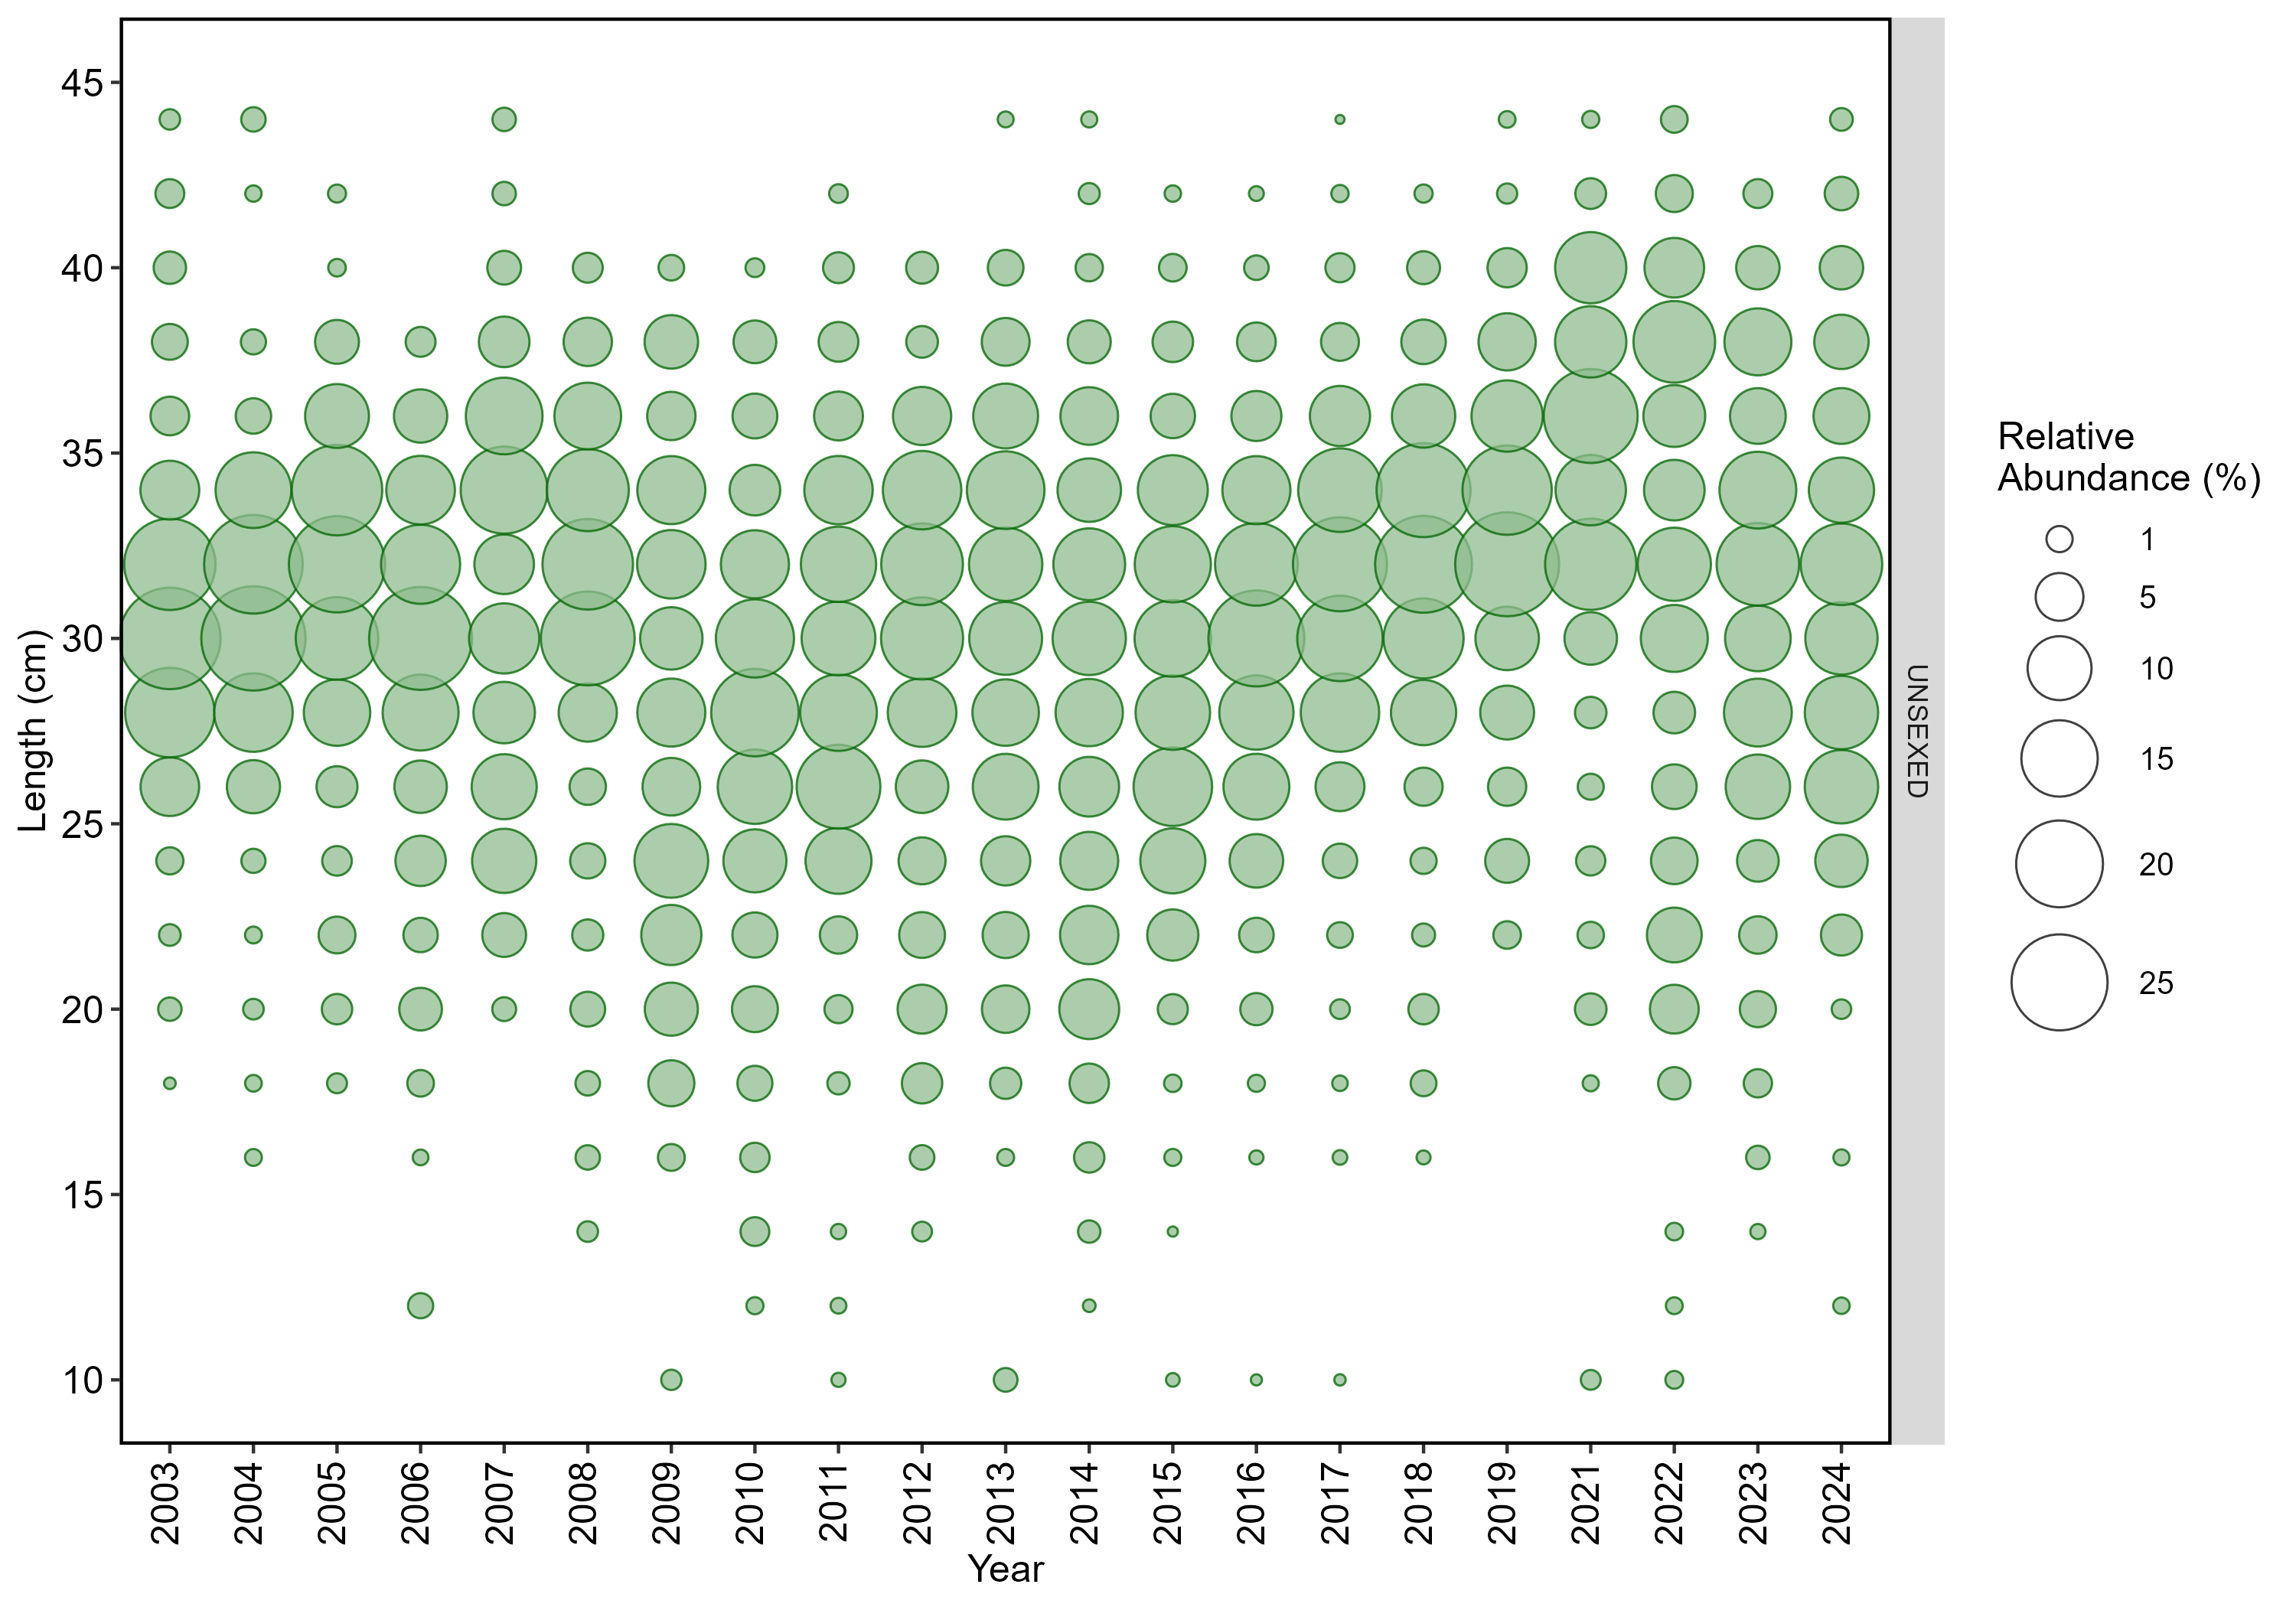
\includegraphics[width=0.95\linewidth,height=\textheight,keepaspectratio]{../plots/wcgbts_comps/plots/flathead sole_length_frequency_sex_0.png}

}

\caption{Length (cm) compostion data from the NWFSC WCGBTS for flathead
sole. Size of the circles within a year indicate higher (larger circles)
and lower (smaller circles) proportion observed by length bin.}

\end{figure}%

\newpage{}

\subsection{Greenspotted rockfish}\label{greenspotted-rockfish}

The most recent assessment of greenspotted rockfish was a benchmark
assessment conducted in 2011. Across available data, greenspotted
rockfish have been observed and sampled by both the NWFSC HKLS and
WCGBTS. The NWFSC HKLS observed greenspotted rockfish at an average of
65 sets per year. The NWFSC WCGBTS observed greenspotted rockfish on an
average of 35 tows per year. For this species, a total of 338 maturity
samples have been collected coastwide (regardless of stock area), with
175 read maturities.

\begingroup\fontsize{10}{12}\selectfont
\begingroup\fontsize{10}{12}\selectfont

\begin{longtable}[t]{>{\raggedleft\arraybackslash}p{2cm}>{\raggedleft\arraybackslash}p{3.5cm}>{\raggedleft\arraybackslash}p{2cm}>{\raggedleft\arraybackslash}p{2cm}>{\raggedleft\arraybackslash}p{2cm}}
\caption{\label{tab:unnamed-chunk-244}Total number of available lengths, read ages, and unread age structures by data source and
state for greenspotted rockfish.}\\
\toprule
State & Source & Lengths & Ages & Age Structures\\
\midrule
\endfirsthead
\caption[]{Total number of available lengths, read ages, and unread age structures by data source and
state for greenspotted rockfish. (\textit{continued)}}\\
\toprule
State & Source & Lengths & Ages & Age Structures\\
\midrule
\endhead

\endfoot
\bottomrule
\endlastfoot
CA & NWFSC HKLS & 6,446 & 843 & 5,408\\
CA & NWFSC WCGBTS & 8,034 & 701 & 4,008\\
OR & NWFSC WCGBTS & 1,366 & 0 & 1,074\\
WA & NWFSC WCGBTS & 45 & 0 & 42\\*
\end{longtable}
\endgroup{}
\endgroup{}

\begin{figure}[H]

{\centering 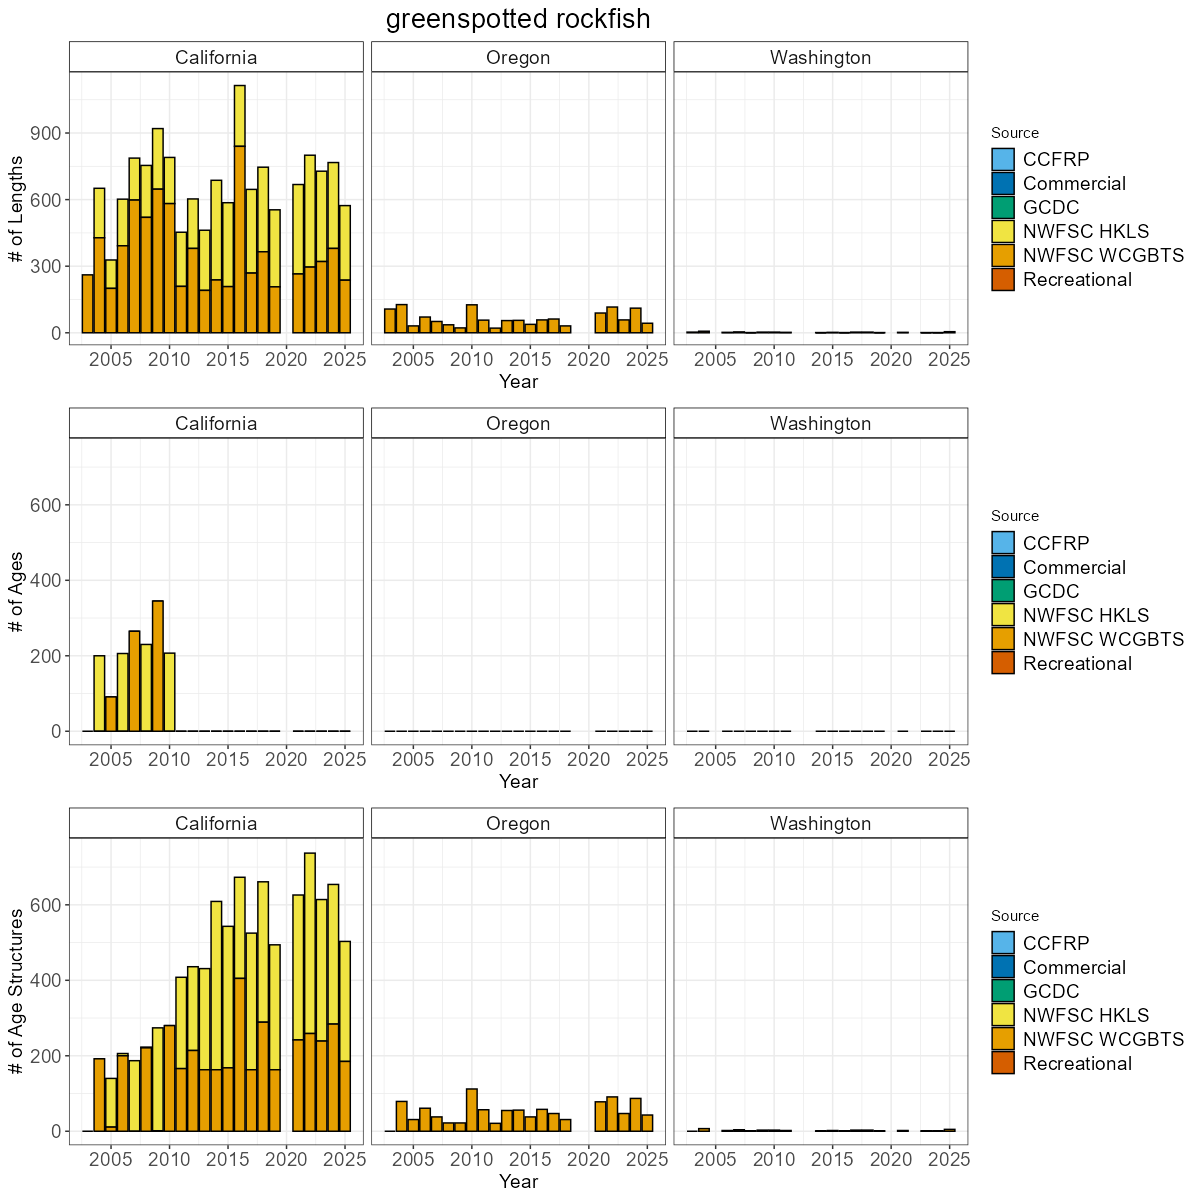
\includegraphics[width=0.95\linewidth,height=\textheight,keepaspectratio]{../plots/state_comparisons/greenspotted_rockfish_state_compositions.png}

}

\caption{Total number of available lengths, read ages, and unread age
structures by data source by year for greenspotted rockfish. Note the
y-axis maximum may differ by data type.}

\end{figure}%

\begin{figure}[H]

{\centering 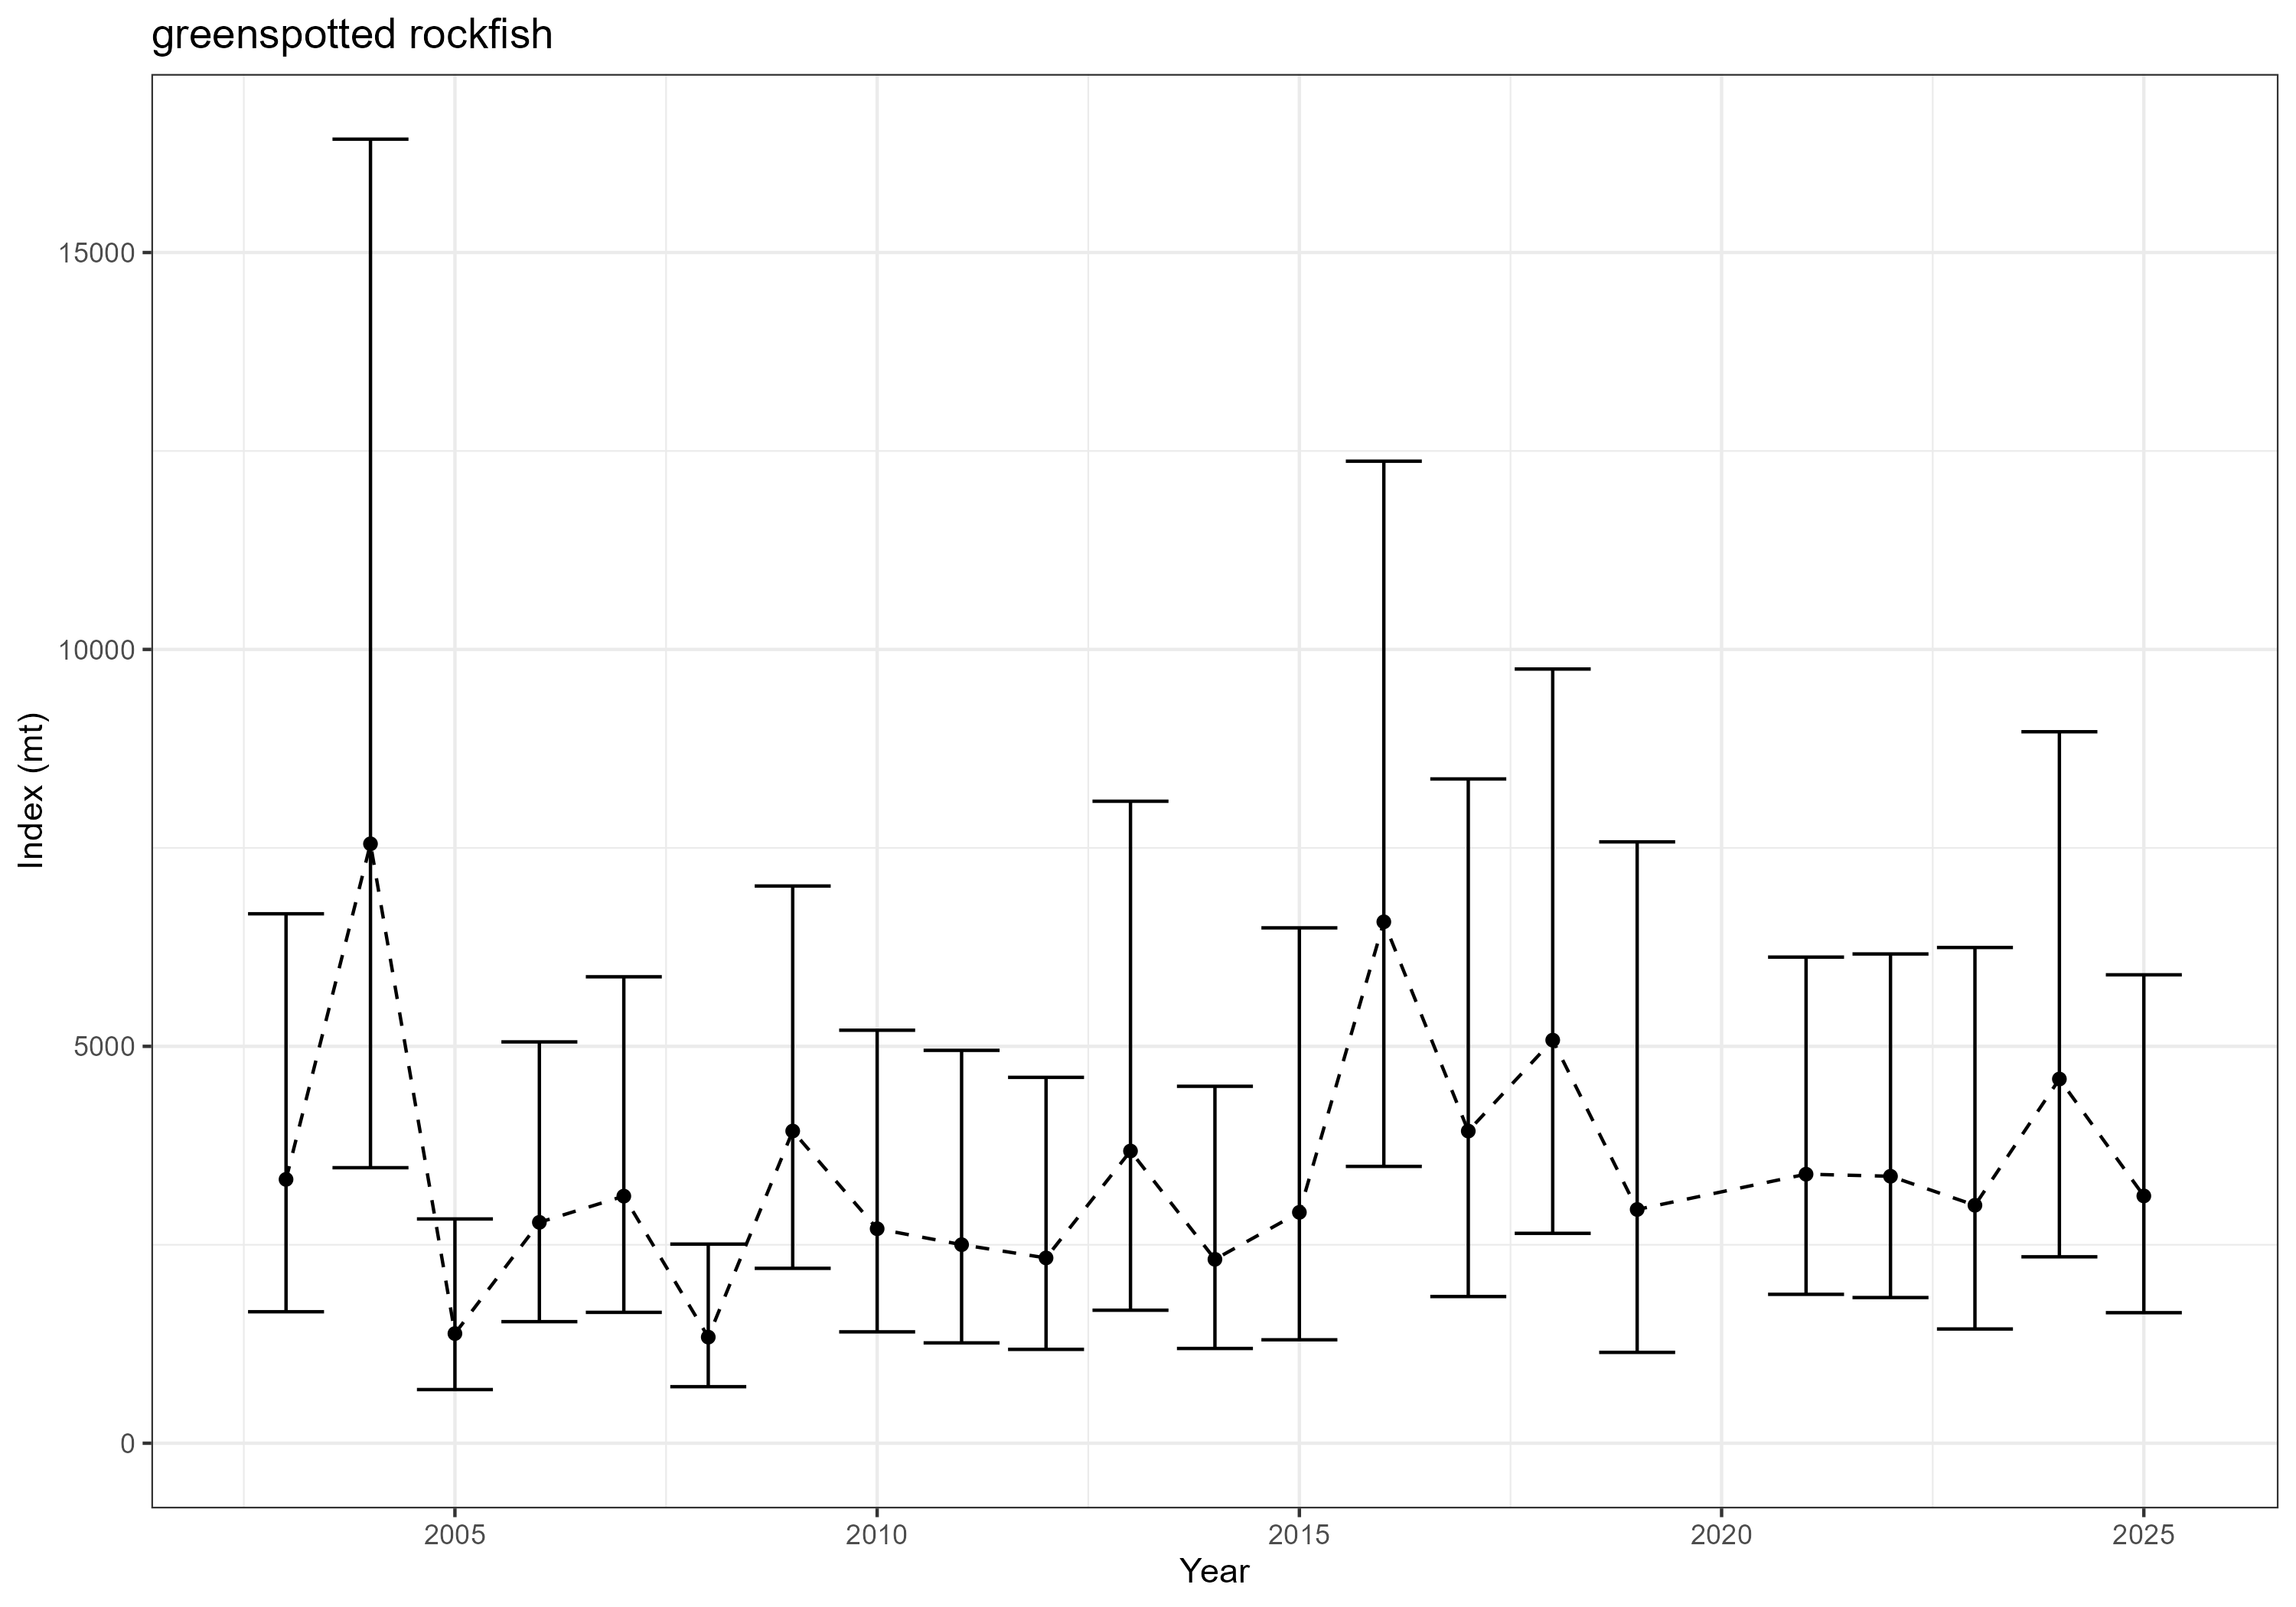
\includegraphics[width=0.95\linewidth,height=\textheight,keepaspectratio]{../plots/wcgbts_indices/greenspotted_rockfish_index.png}

}

\caption{Estimated relative index of abundance for greenspotted rockfish
from the NWFSC WCGBTS.}

\end{figure}%

\begin{figure}[H]

{\centering 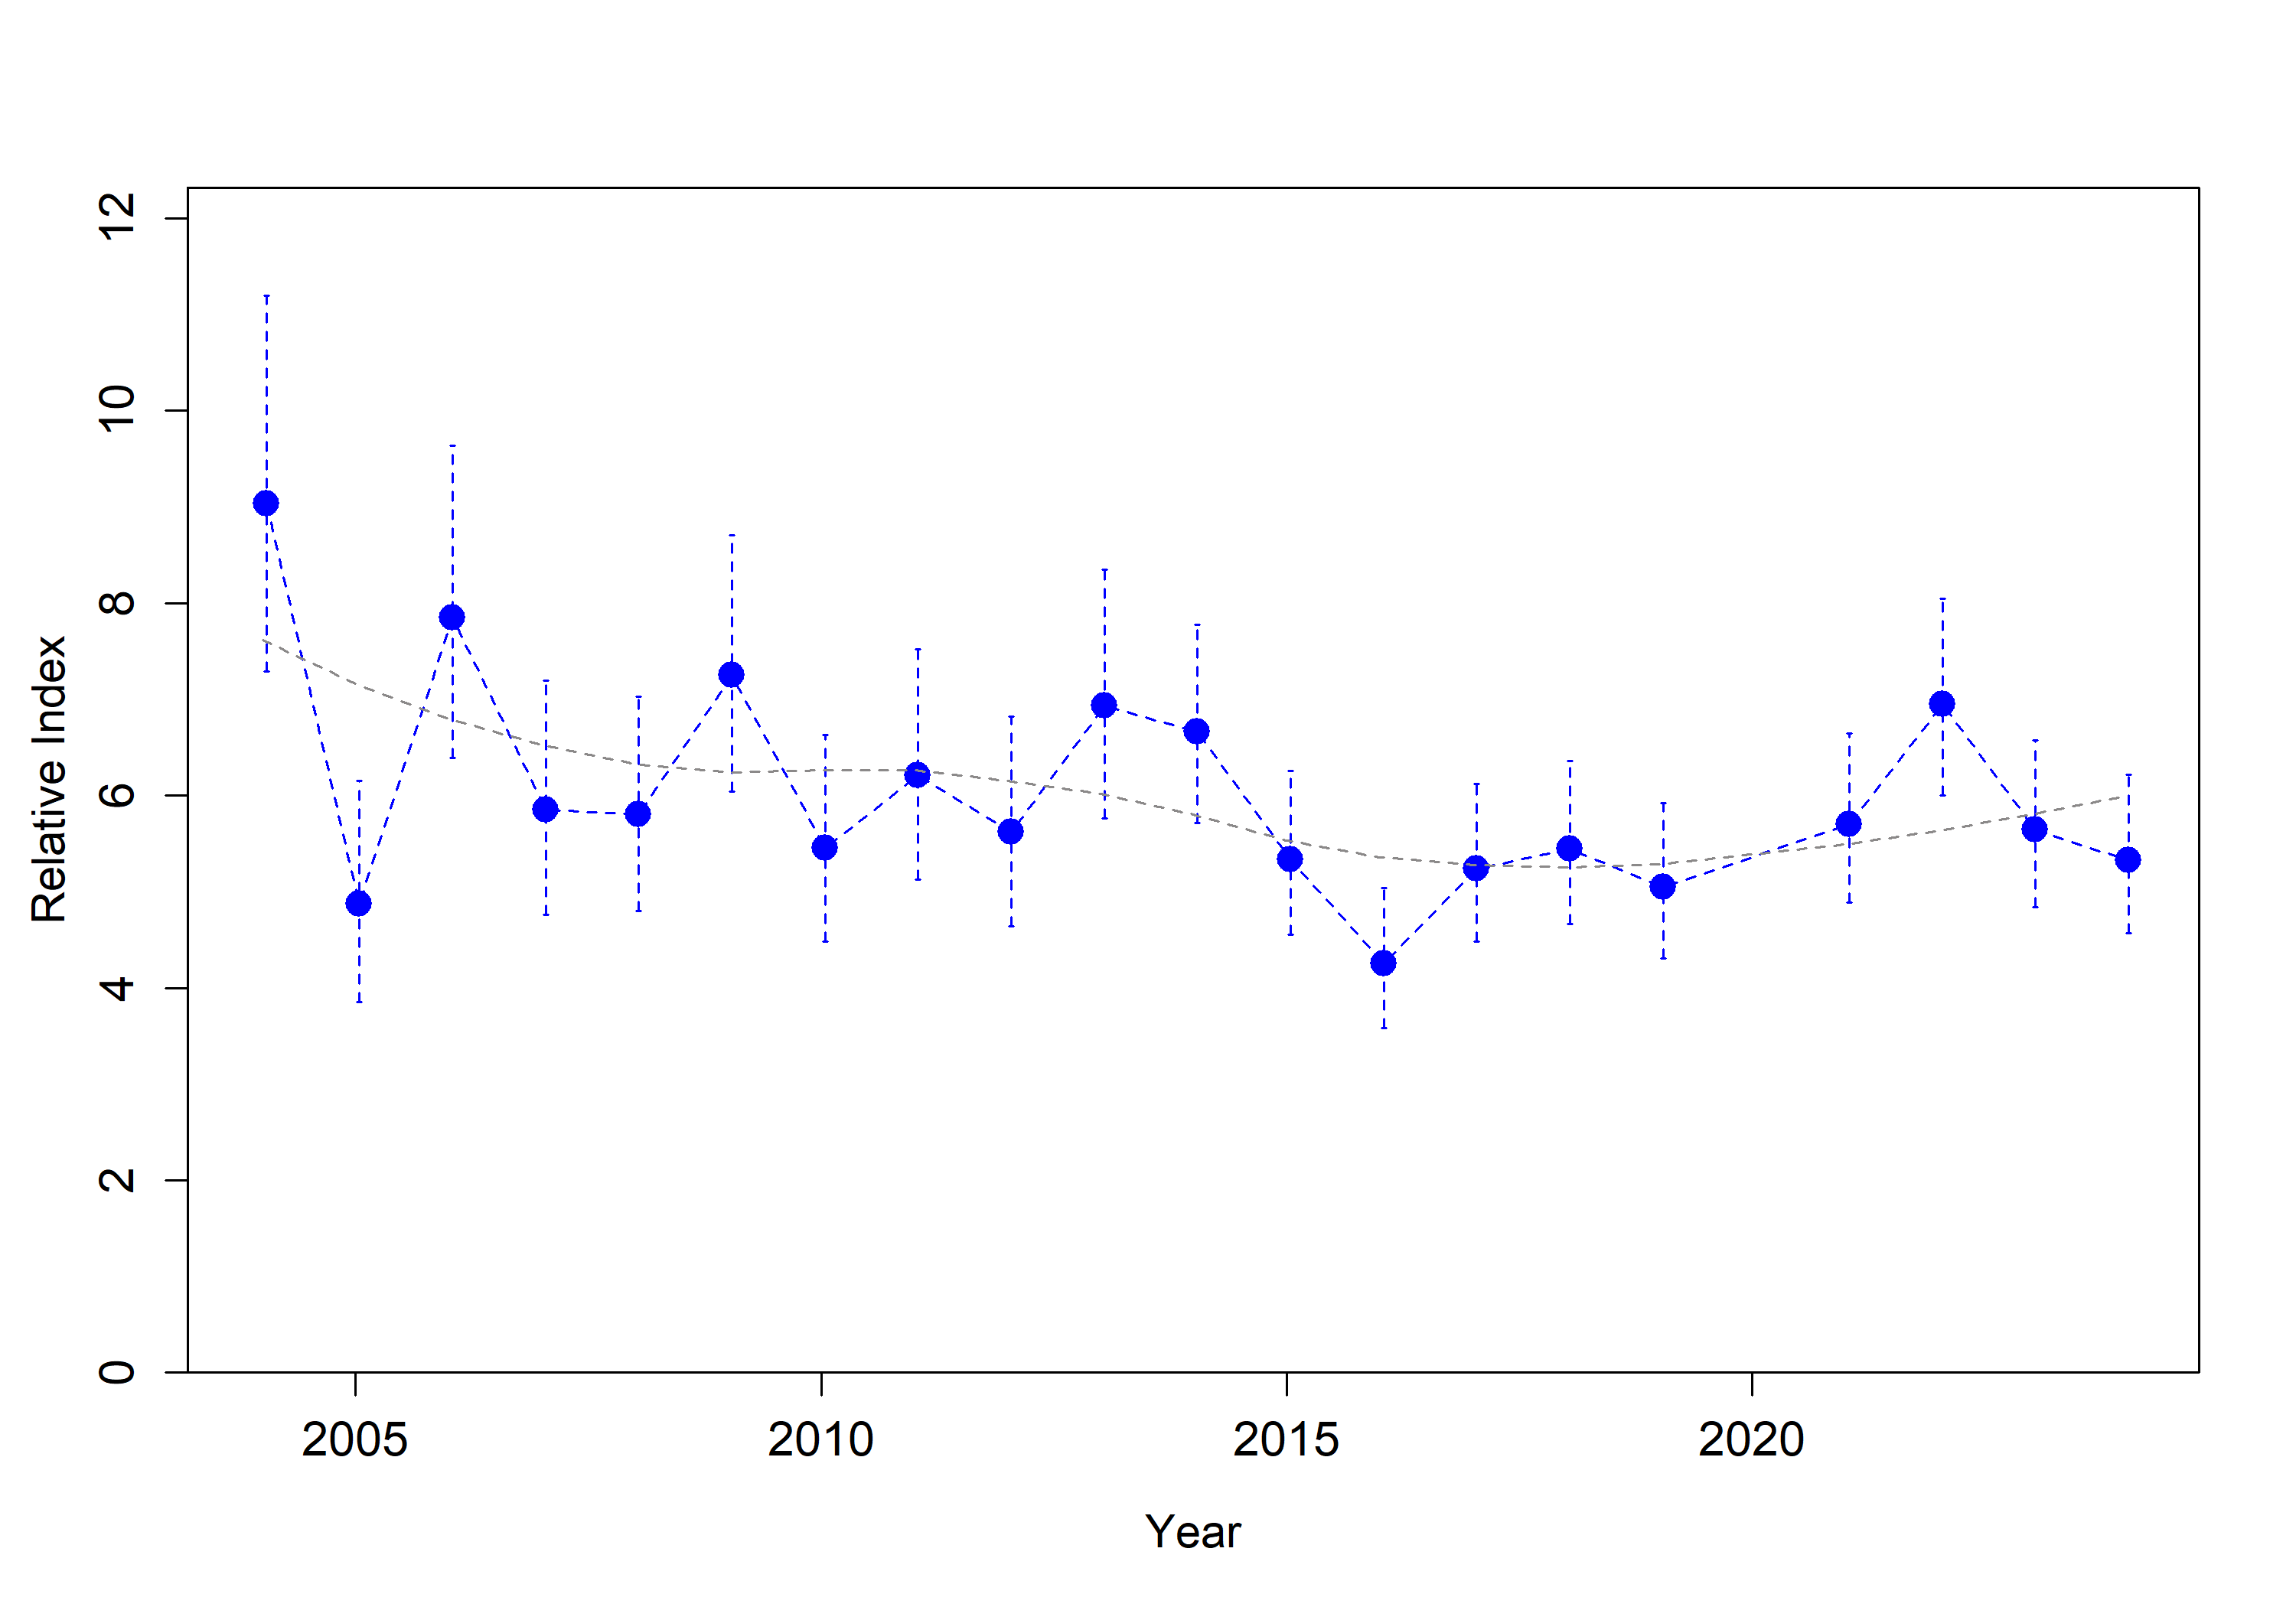
\includegraphics[width=0.95\linewidth,height=\textheight,keepaspectratio]{../plots/hkl_indices/greenspotted rockfish_negbinom index.png}

}

\caption{Estimated relative index of abundance for greenspotted rockfish
from the NWFSC HKLS.}

\end{figure}%

\begin{figure}[H]

{\centering 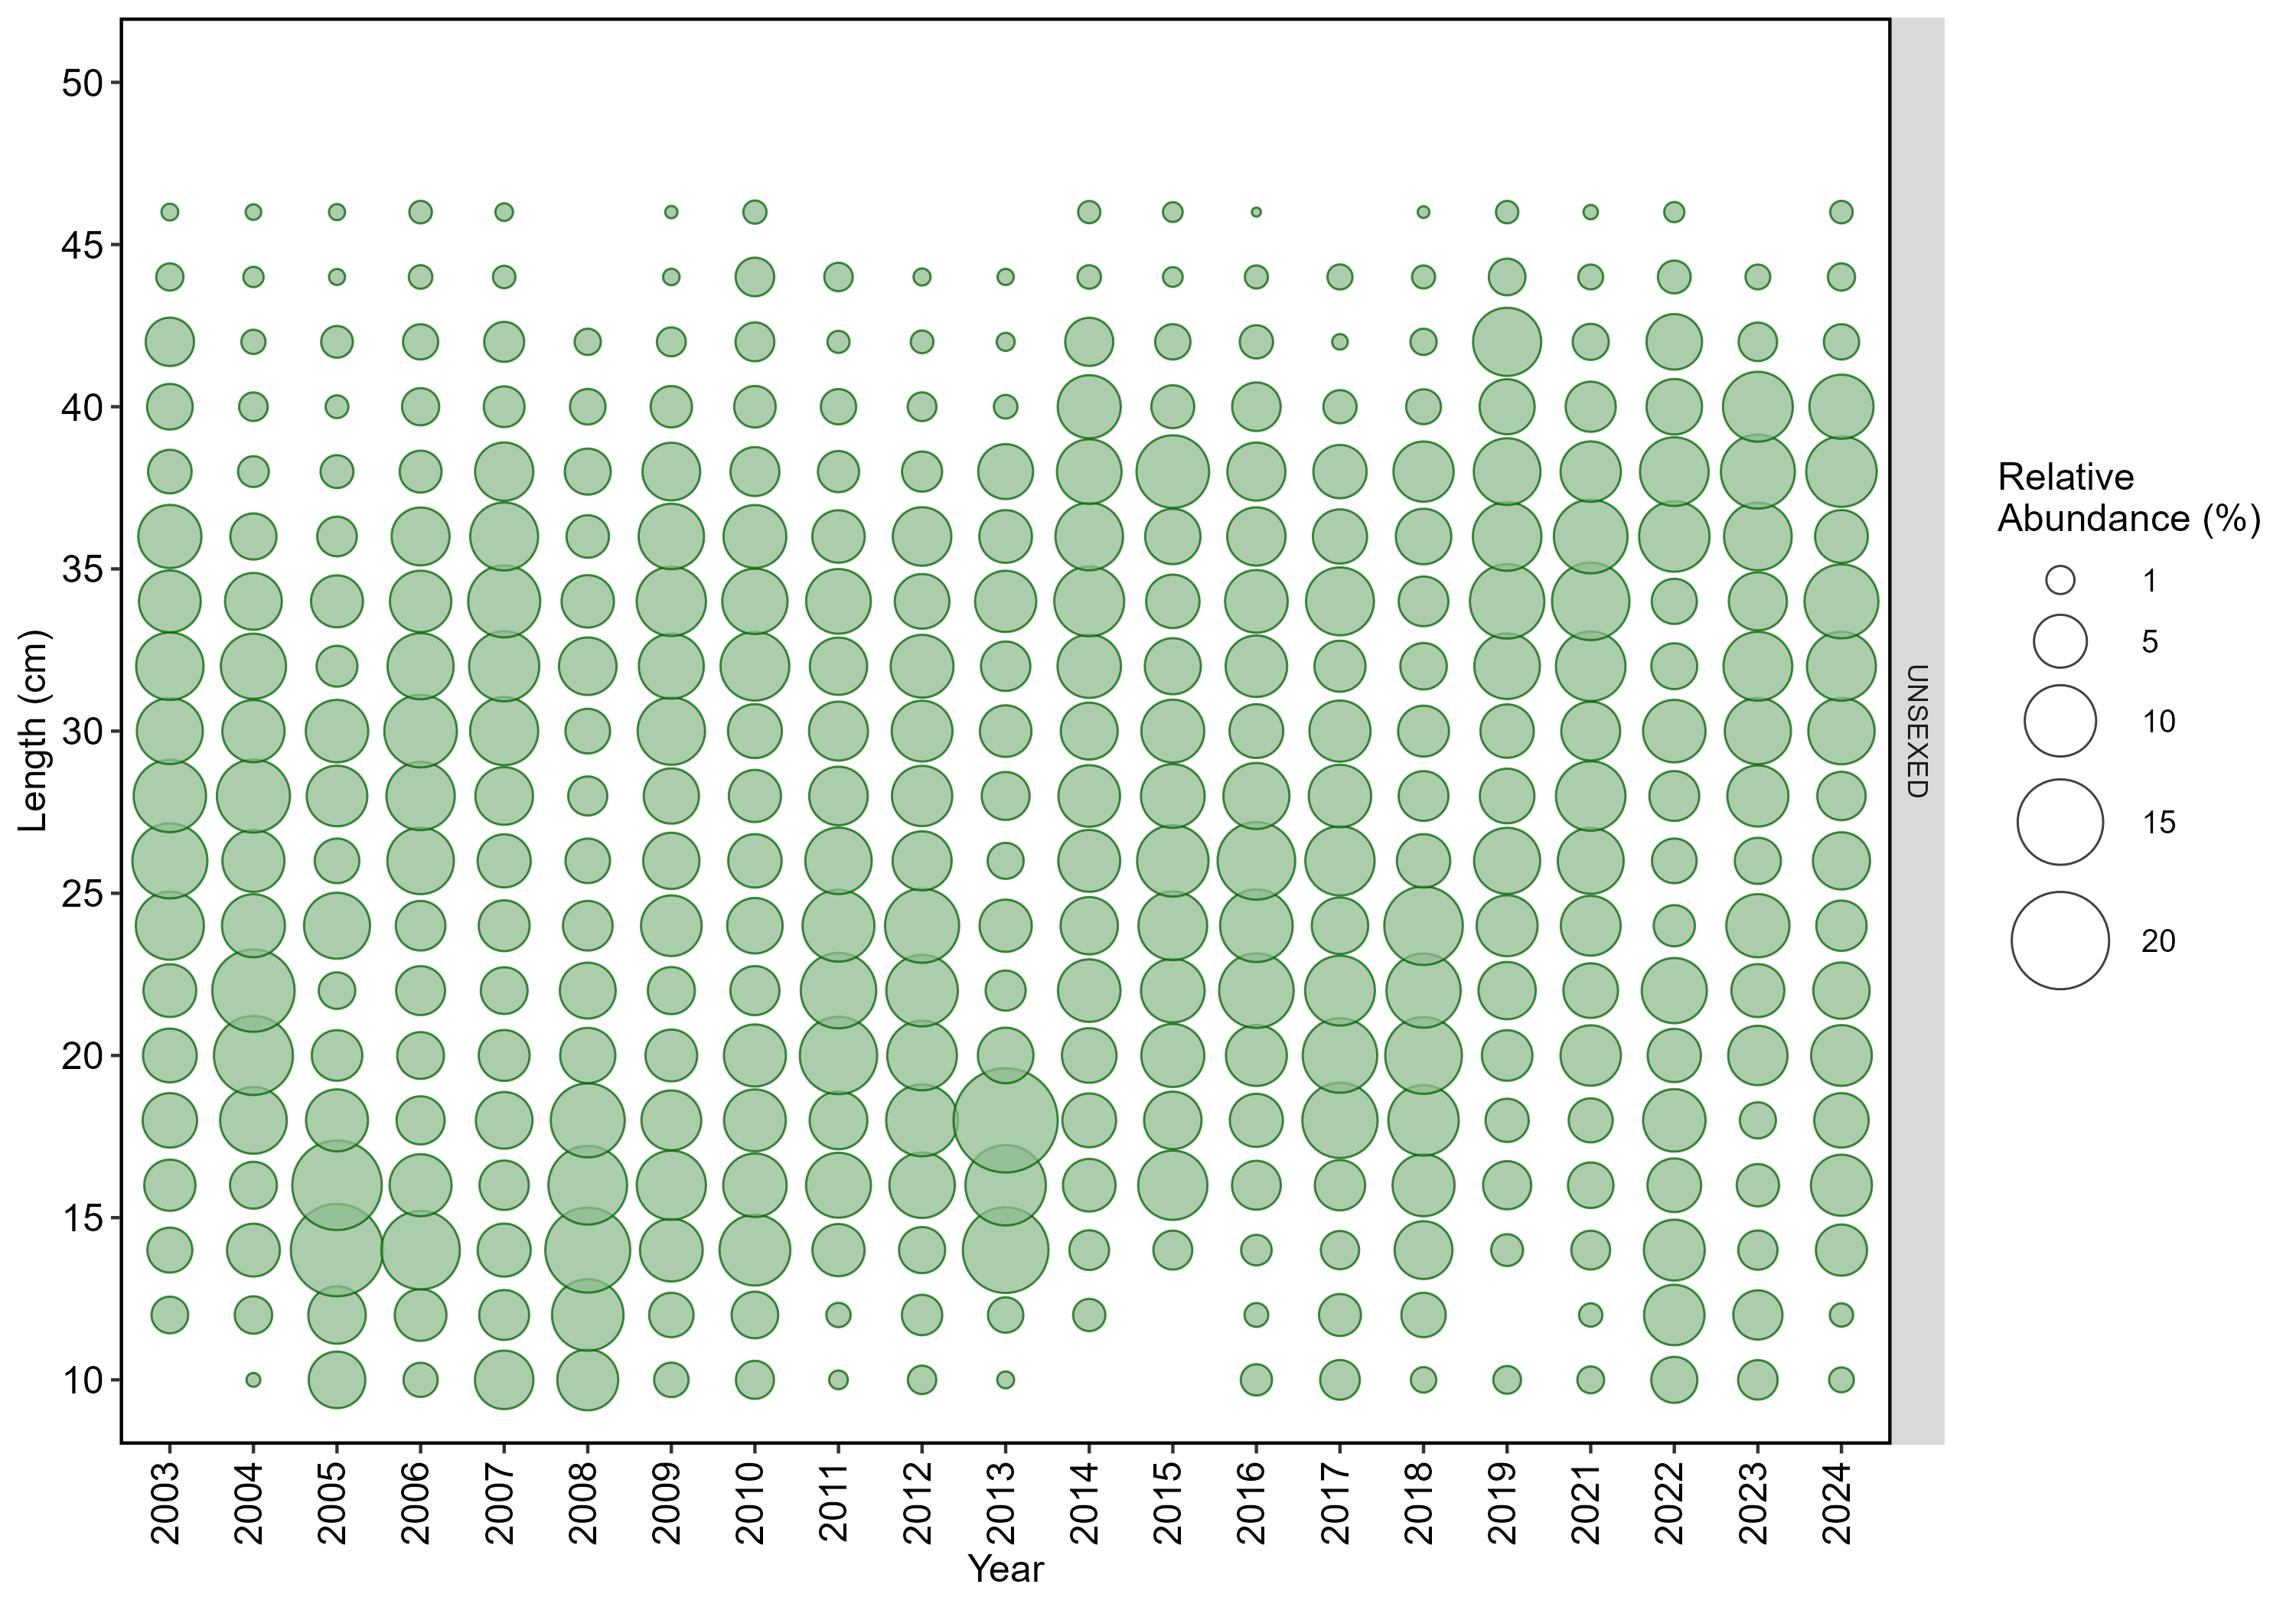
\includegraphics[width=0.95\linewidth,height=\textheight,keepaspectratio]{../plots/wcgbts_comps/plots/greenspotted rockfish_length_frequency_sex_0.png}

}

\caption{Length (cm) compostion data from the NWFSC WCGBTS for
greenspotted rockfish. Size of the circles within a year indicate higher
(larger circles) and lower (smaller circles) proportion observed by
length bin.}

\end{figure}%

\begin{figure}[H]

{\centering 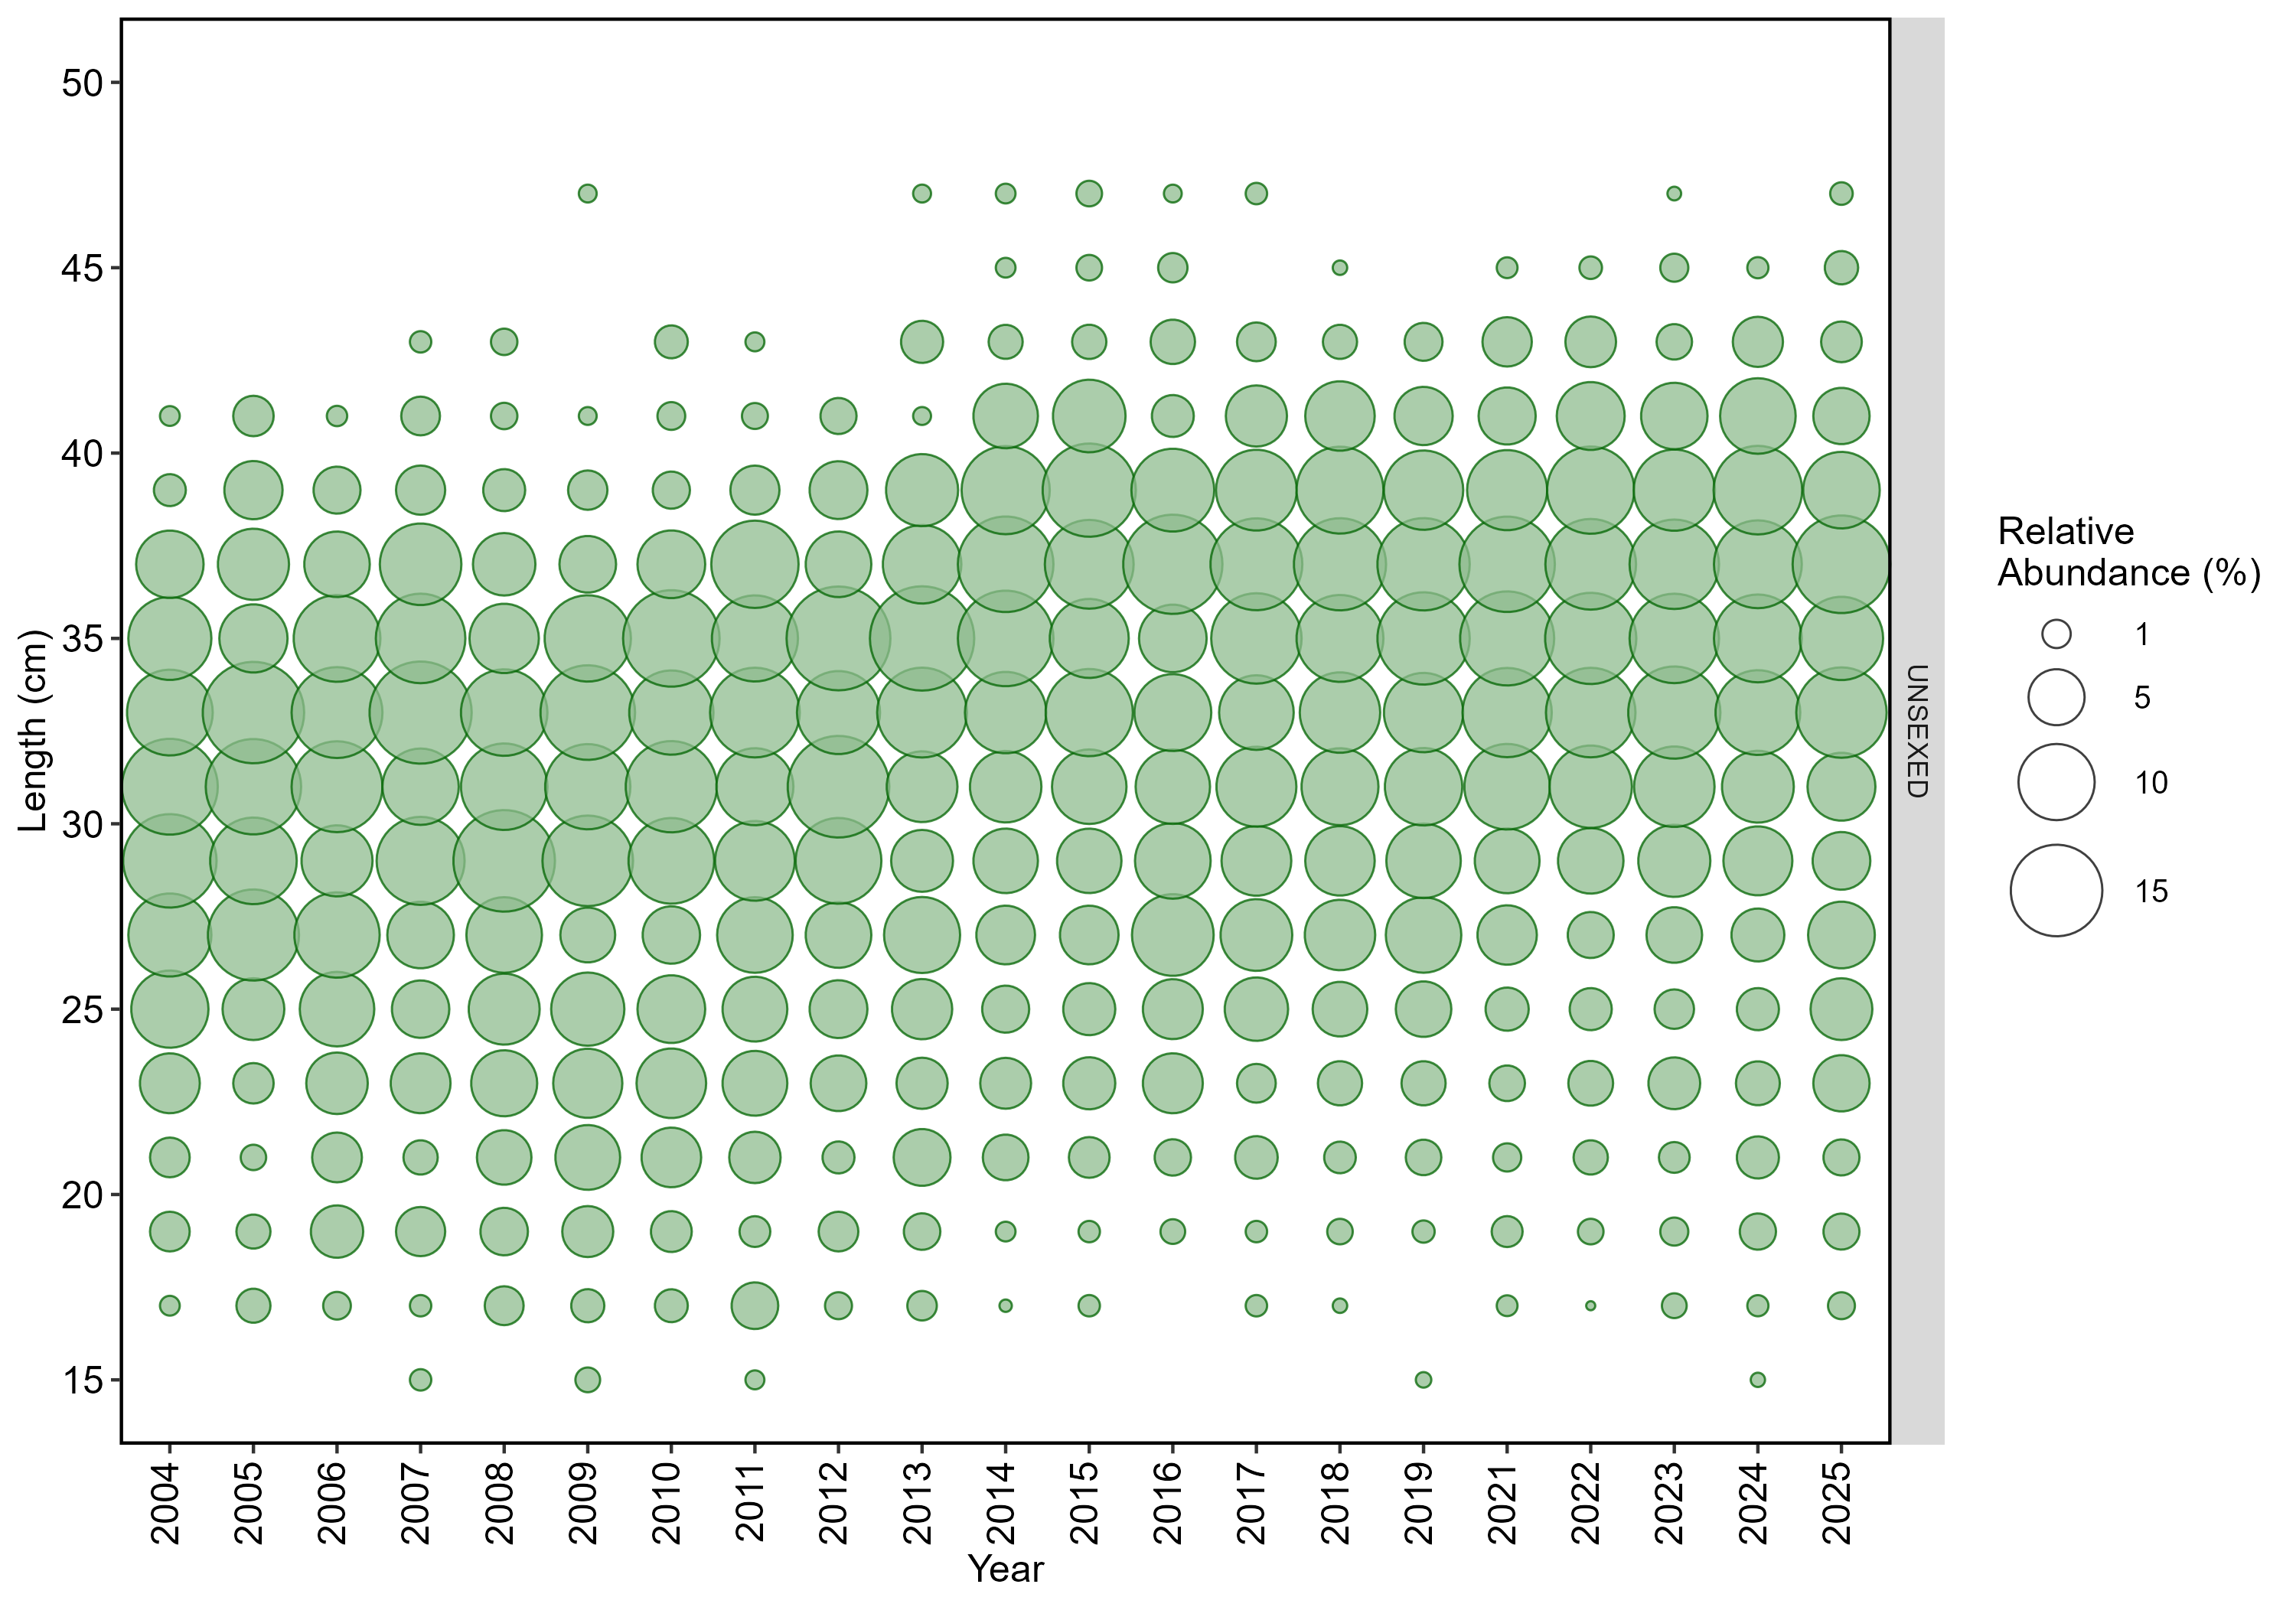
\includegraphics[width=0.95\linewidth,height=\textheight,keepaspectratio]{../plots/hkl_comps/plots/greenspotted rockfish_nwfsc_hkl_length_frequency_sex_0.png}

}

\caption{Length (cm) compostion data from the NWFSC HKLS for
greenspotted rockfish. Size of the circles within a year indicate higher
(larger circles) and lower (smaller circles) proportion observed by
length bin.}

\end{figure}%

\newpage{}

\subsection{Greenstriped rockfish}\label{greenstriped-rockfish}

The most recent assessment of greenstriped rockfish was a benchmark
assessment conducted in 2009. Across available data, greenstriped
rockfish have been observed and sampled by both the NWFSC HKLS and
WCGBTS. The NWFSC HKLS observed greenstriped rockfish at an average of
28 sets per year. The NWFSC WCGBTS observed greenstriped rockfish on an
average of 161 tows per year. For this species, a total of 73 maturity
samples have been collected coastwide (regardless of stock area), with
73 read maturities.

\begingroup\fontsize{10}{12}\selectfont
\begingroup\fontsize{10}{12}\selectfont

\begin{longtable}[t]{>{\raggedleft\arraybackslash}p{2cm}>{\raggedleft\arraybackslash}p{3.5cm}>{\raggedleft\arraybackslash}p{2cm}>{\raggedleft\arraybackslash}p{2cm}>{\raggedleft\arraybackslash}p{2cm}}
\caption{\label{tab:unnamed-chunk-261}Total number of available lengths, read ages, and unread age structures by data source and
state for greenstriped rockfish.}\\
\toprule
State & Source & Lengths & Ages & Age Structures\\
\midrule
\endfirsthead
\caption[]{Total number of available lengths, read ages, and unread age structures by data source and
state for greenstriped rockfish. (\textit{continued)}}\\
\toprule
State & Source & Lengths & Ages & Age Structures\\
\midrule
\endhead

\endfoot
\bottomrule
\endlastfoot
CA & NWFSC HKLS & 1,315 & 0 & 1,302\\
CA & NWFSC WCGBTS & 17,531 & 1,359 & 4,458\\
OR & NWFSC WCGBTS & 20,348 & 1,346 & 4,169\\
WA & NWFSC WCGBTS & 10,619 & 709 & 2,012\\*
\end{longtable}
\endgroup{}
\endgroup{}

\begin{figure}[H]

{\centering 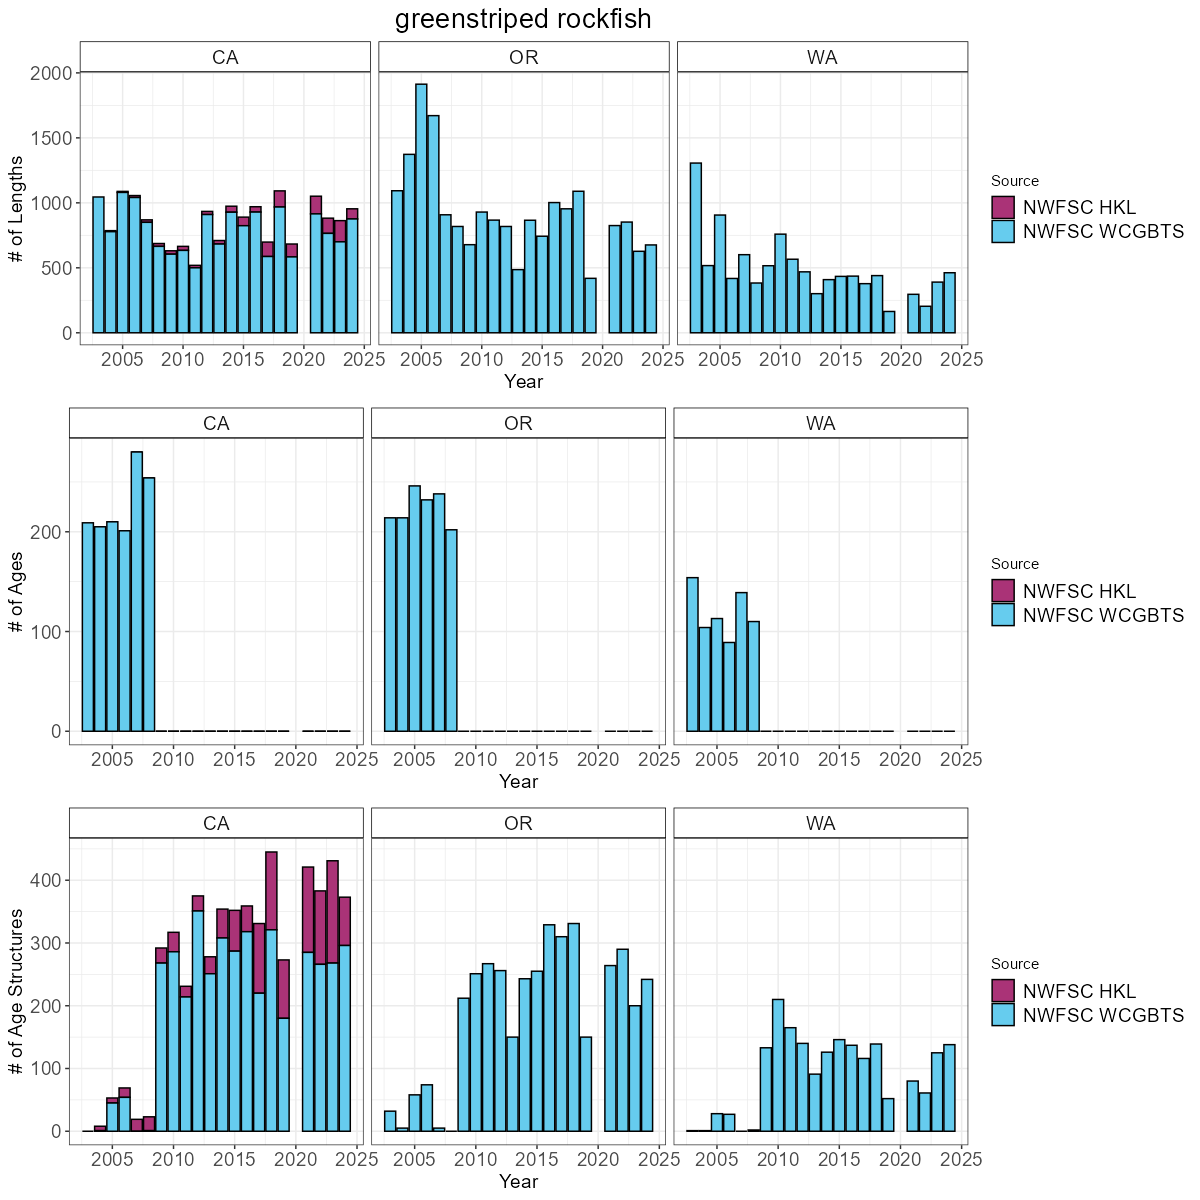
\includegraphics[width=0.95\linewidth,height=\textheight,keepaspectratio]{../plots/state_comparisons/greenstriped_rockfish_state_compositions.png}

}

\caption{Total number of available lengths, read ages, and unread age
structures by data source by year for greenstriped rockfish. Note the
y-axis maximum may differ by data type.}

\end{figure}%

\begin{figure}[H]

{\centering 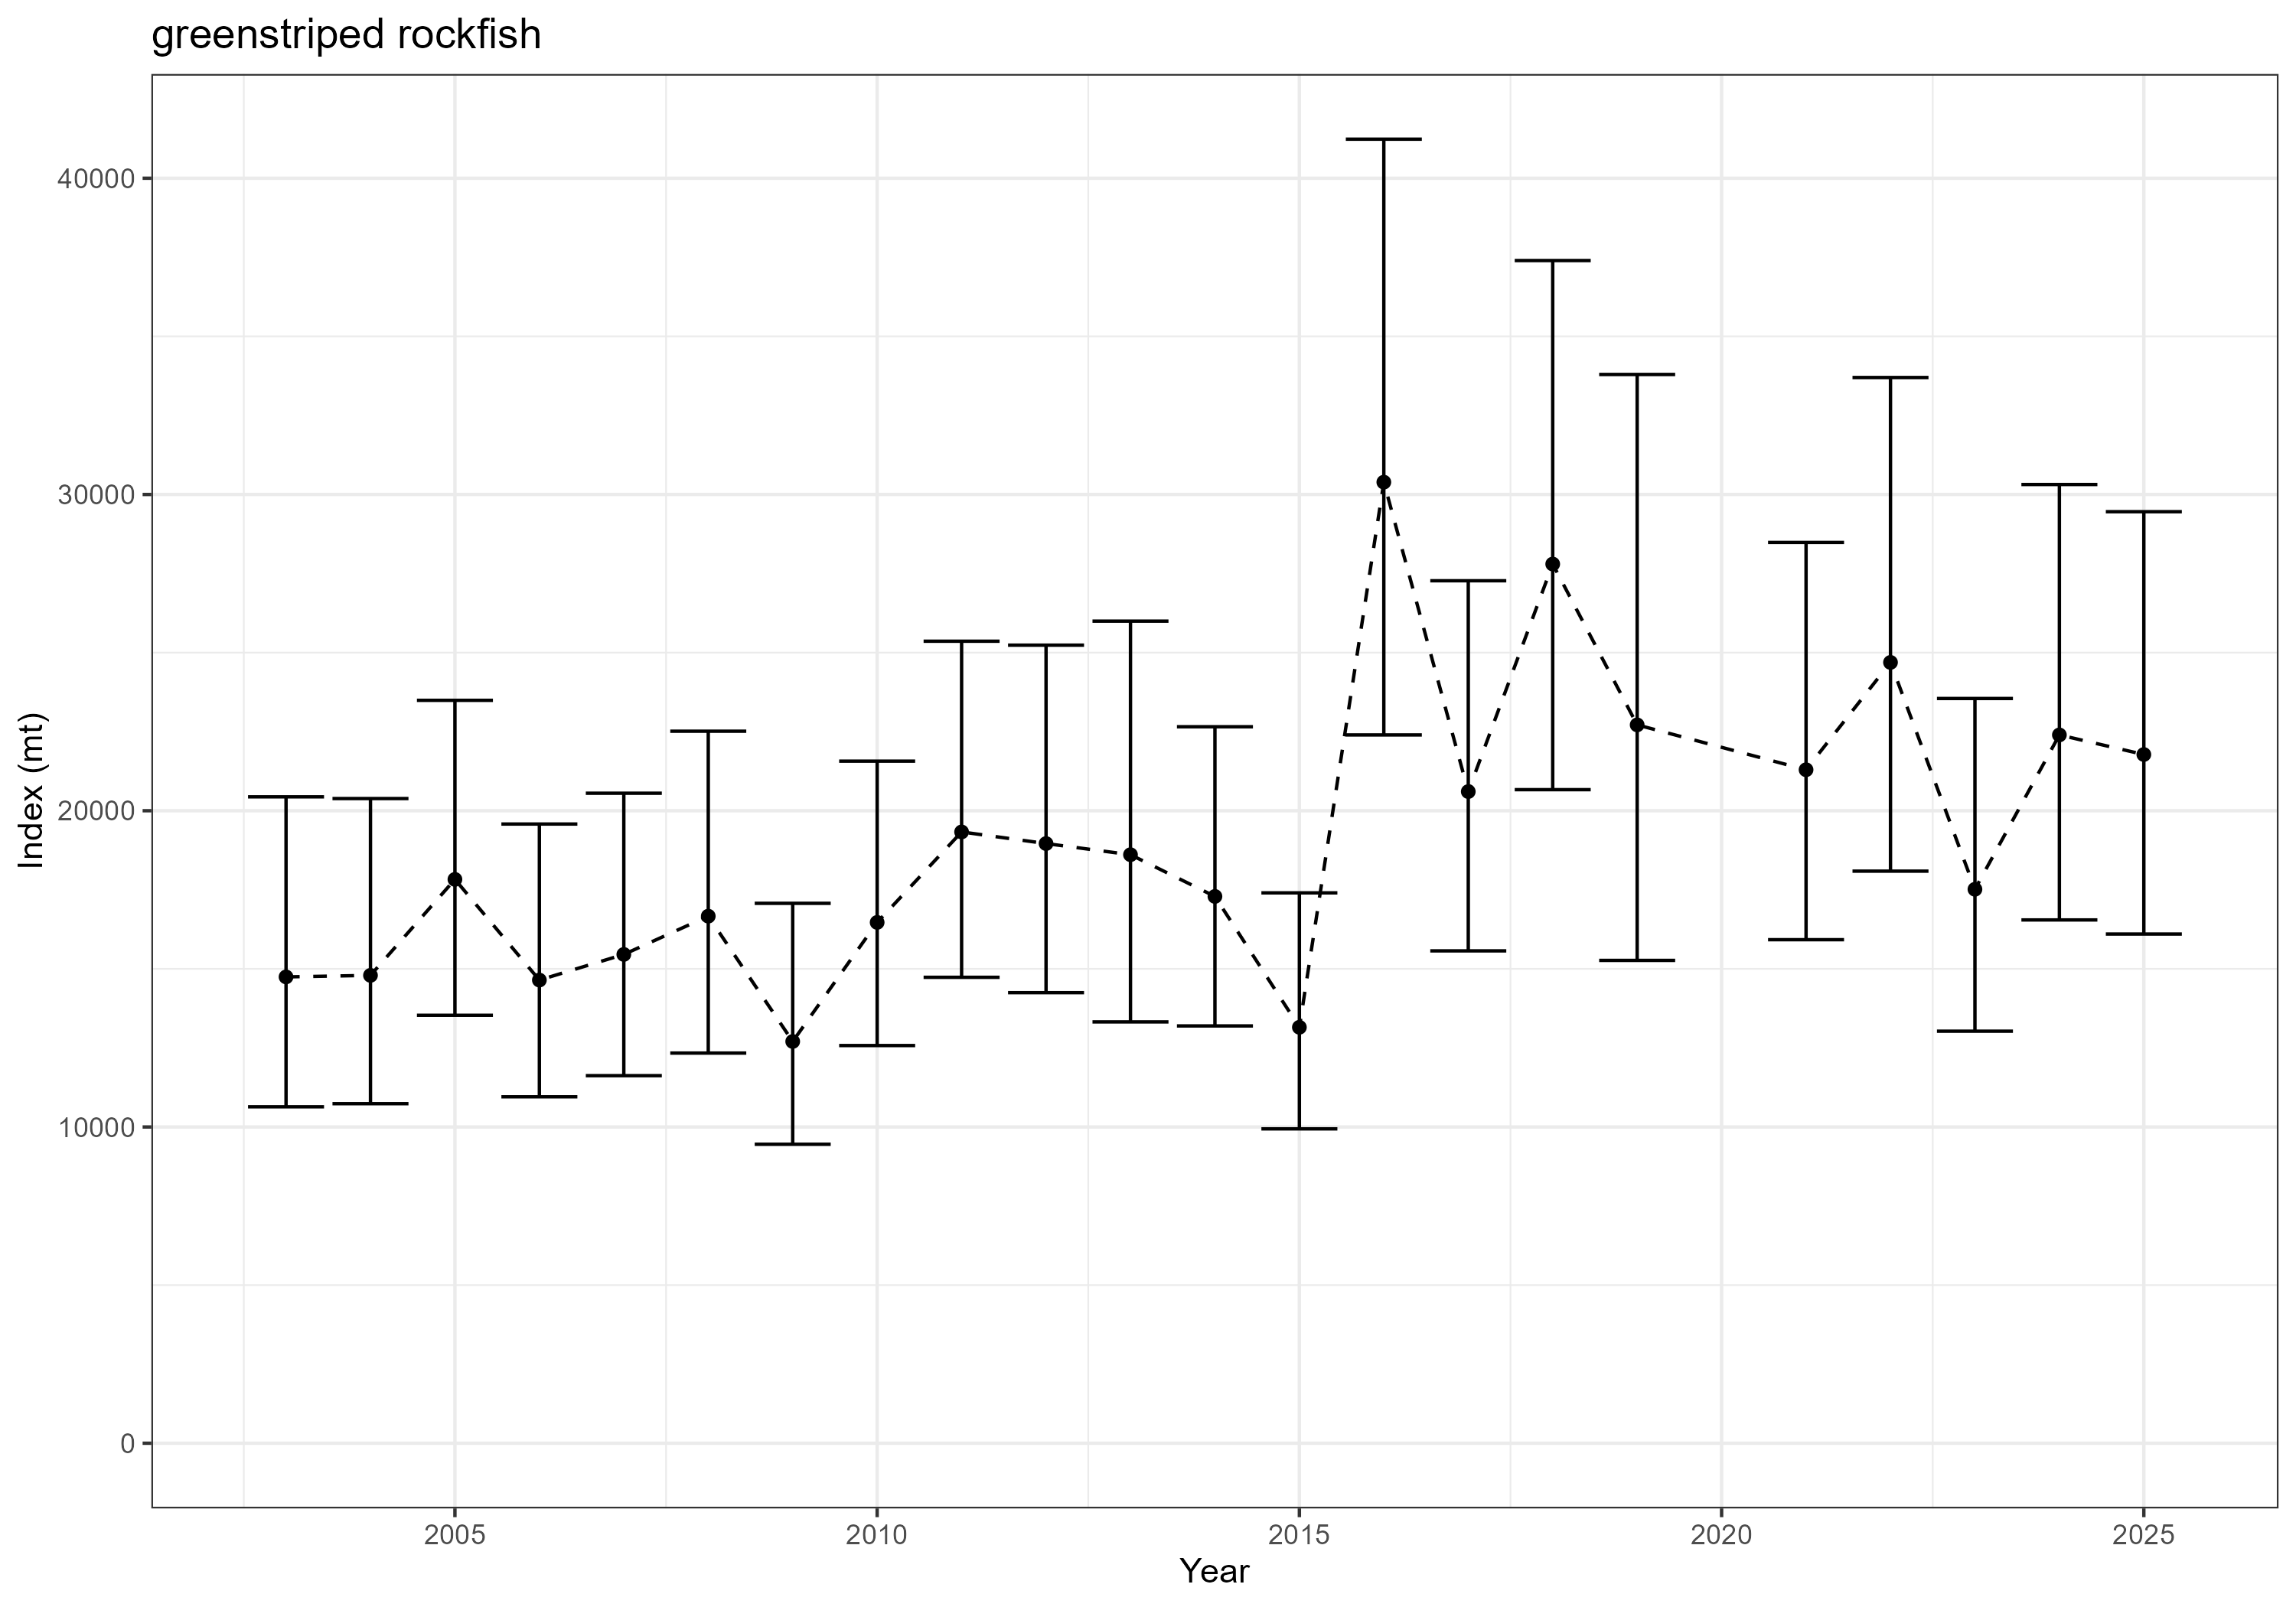
\includegraphics[width=0.95\linewidth,height=\textheight,keepaspectratio]{../plots/wcgbts_indices/greenstriped_rockfish_index.png}

}

\caption{Estimated relative index of abundance for greenstriped rockfish
from the NWFSC WCGBTS.}

\end{figure}%

\begin{figure}[H]

{\centering 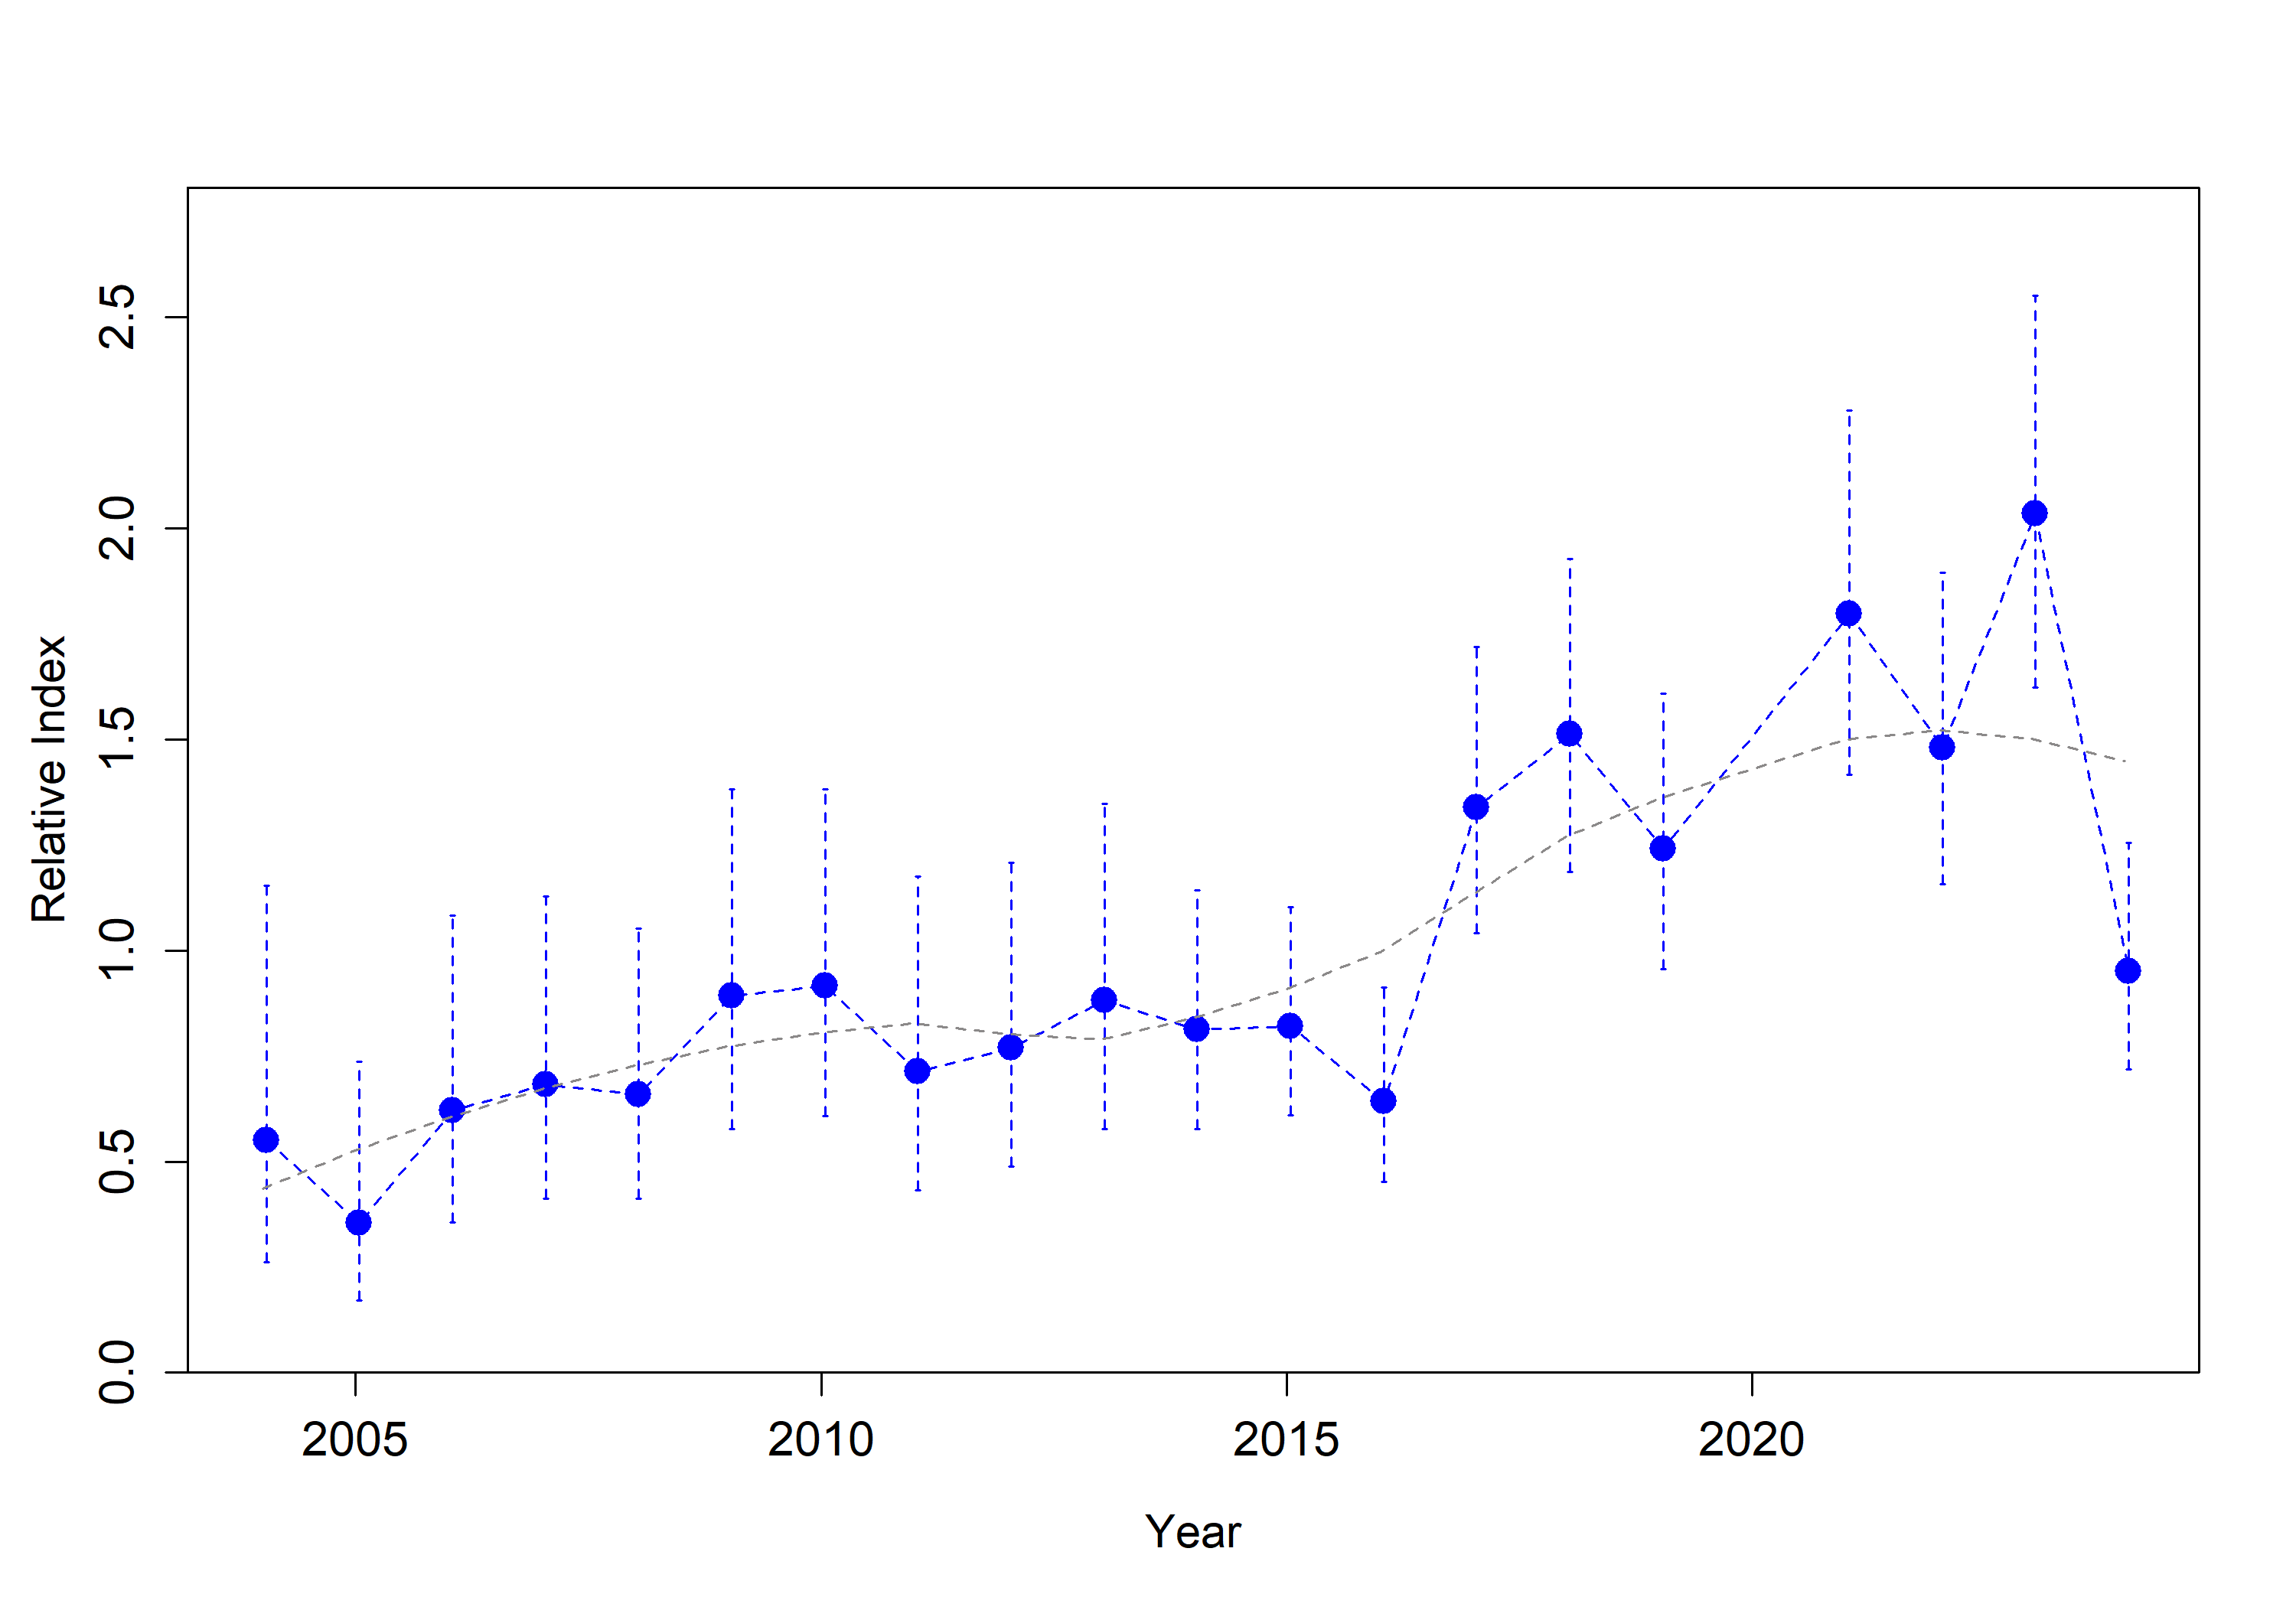
\includegraphics[width=0.95\linewidth,height=\textheight,keepaspectratio]{../plots/hkl_indices/greenstriped rockfish_negbinom index.png}

}

\caption{Estimated relative index of abundance for greenstriped rockfish
from the NWFSC HKLS.}

\end{figure}%

\begin{figure}[H]

{\centering 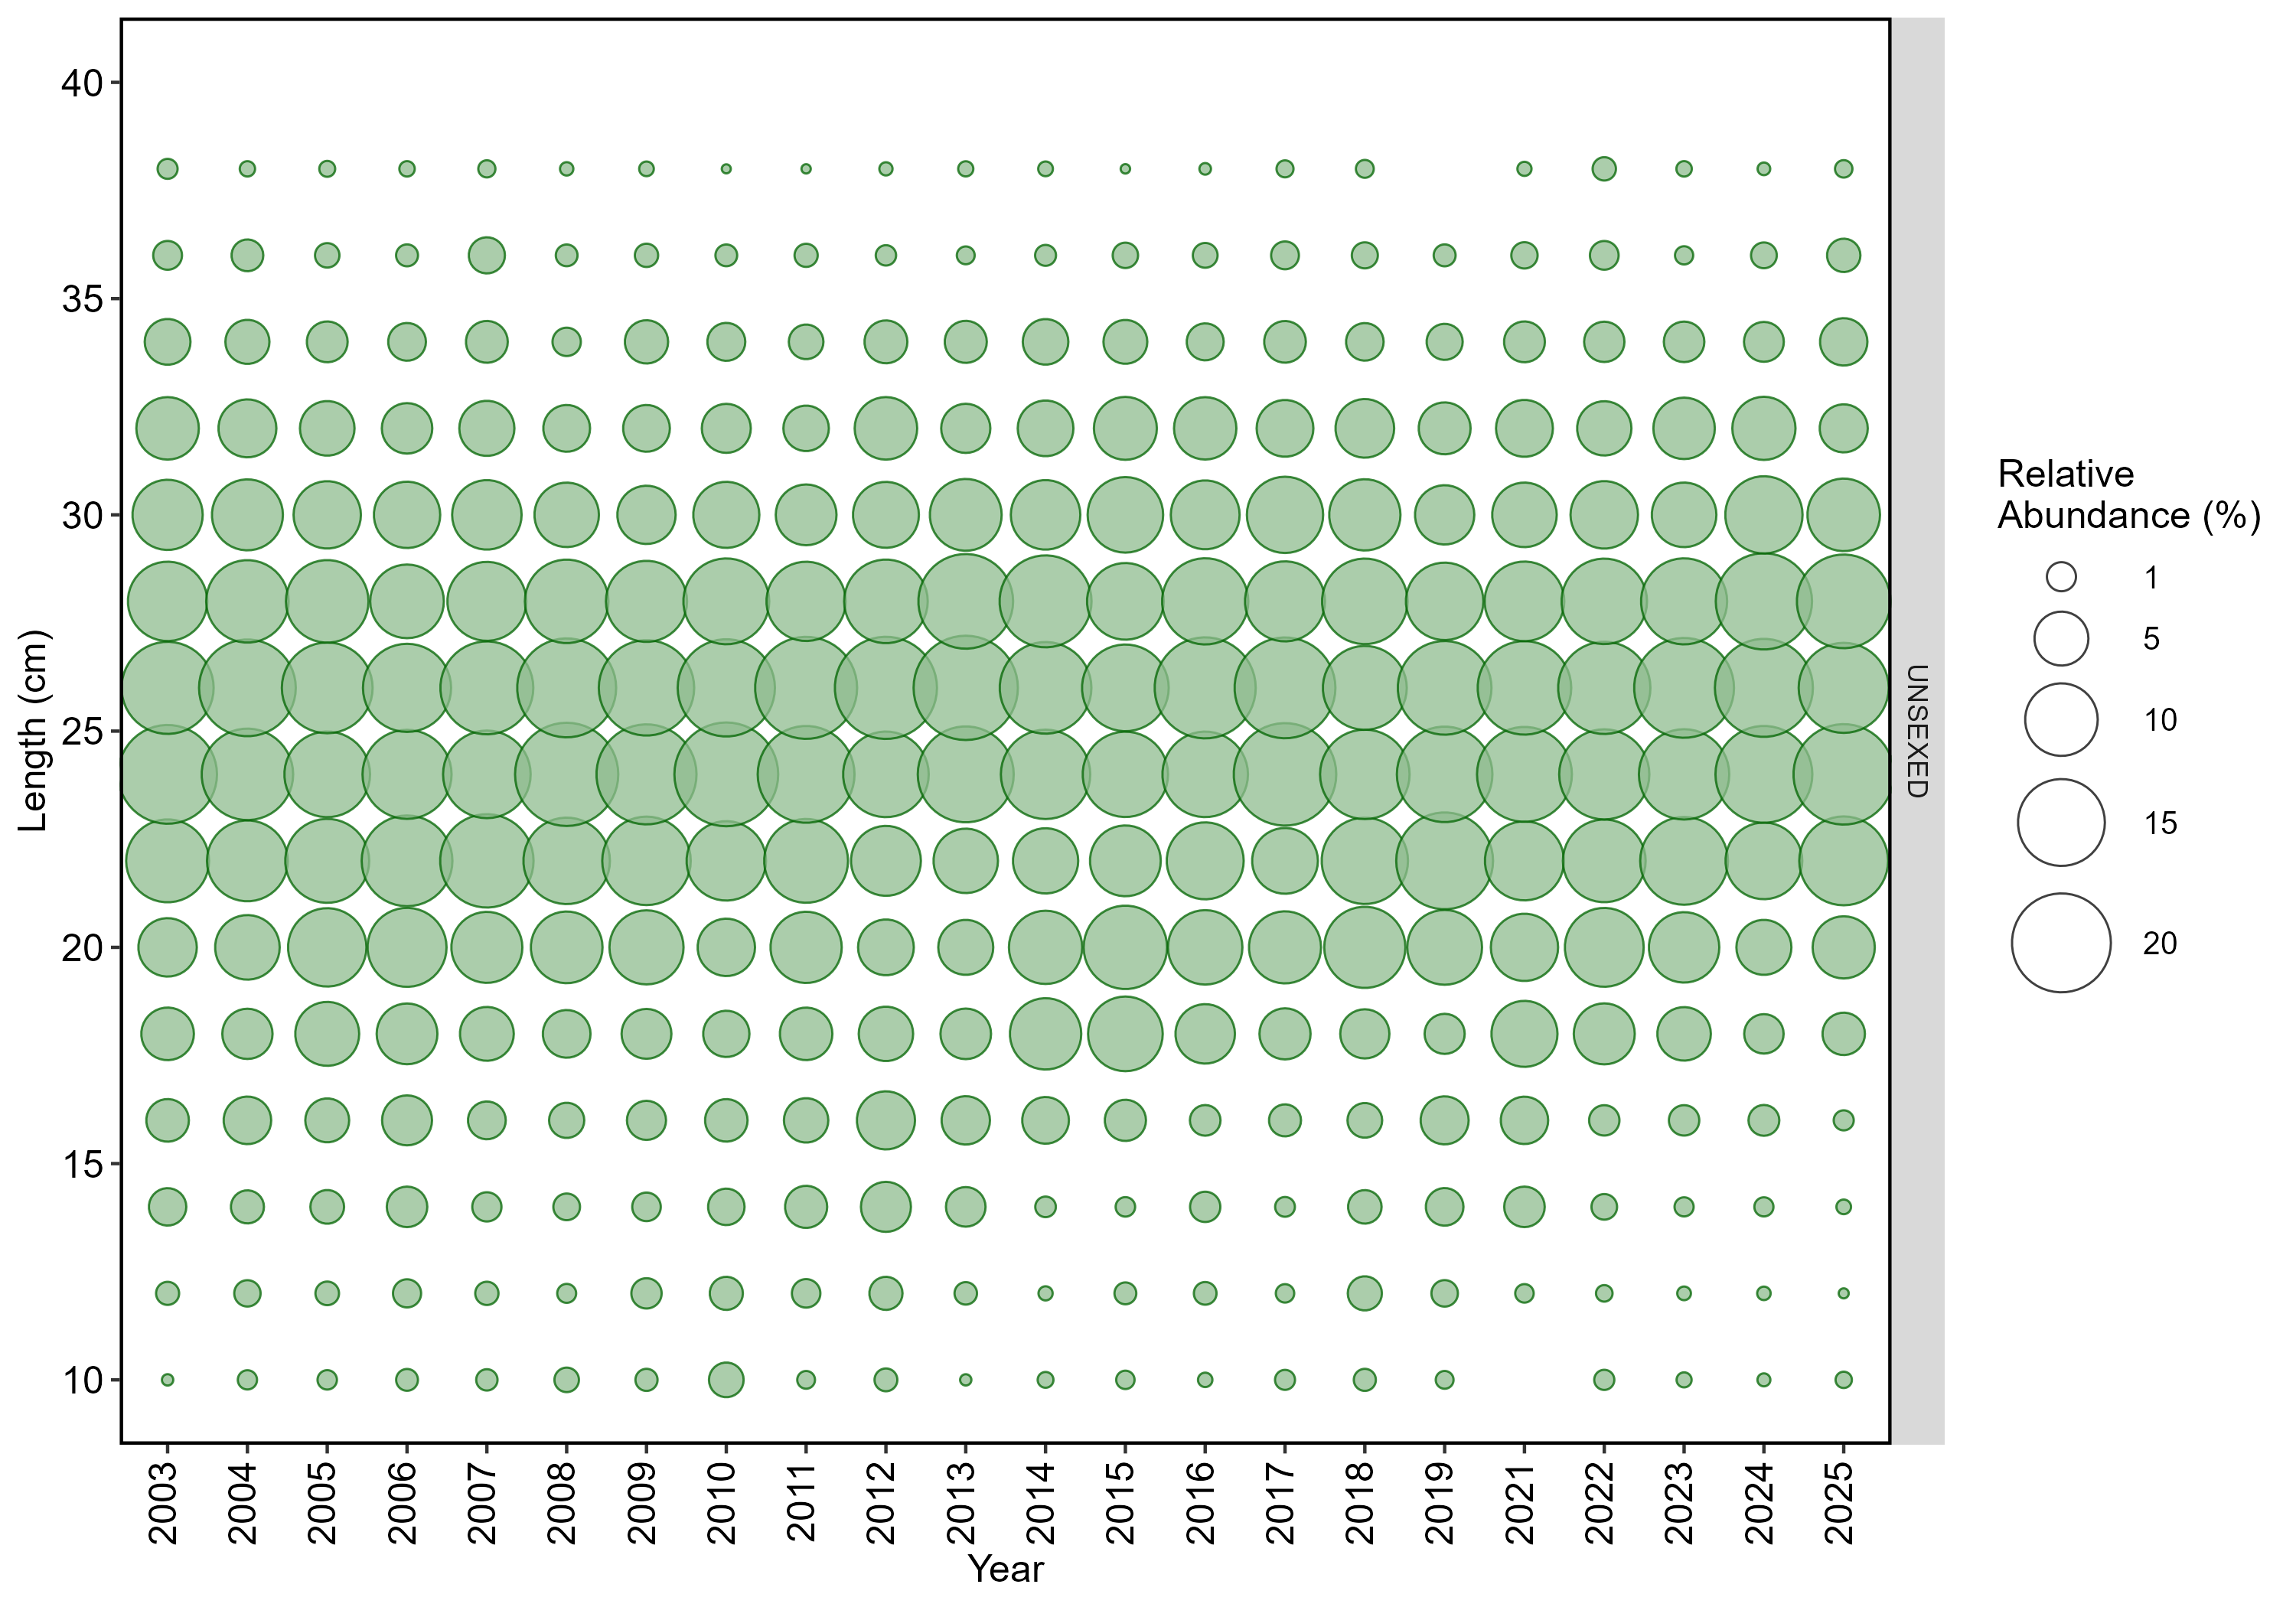
\includegraphics[width=0.95\linewidth,height=\textheight,keepaspectratio]{../plots/wcgbts_comps/plots/greenstriped rockfish_length_frequency_sex_0.png}

}

\caption{Length (cm) compostion data from the NWFSC WCGBTS for
greenstriped rockfish. Size of the circles within a year indicate higher
(larger circles) and lower (smaller circles) proportion observed by
length bin.}

\end{figure}%

\begin{figure}[H]

{\centering 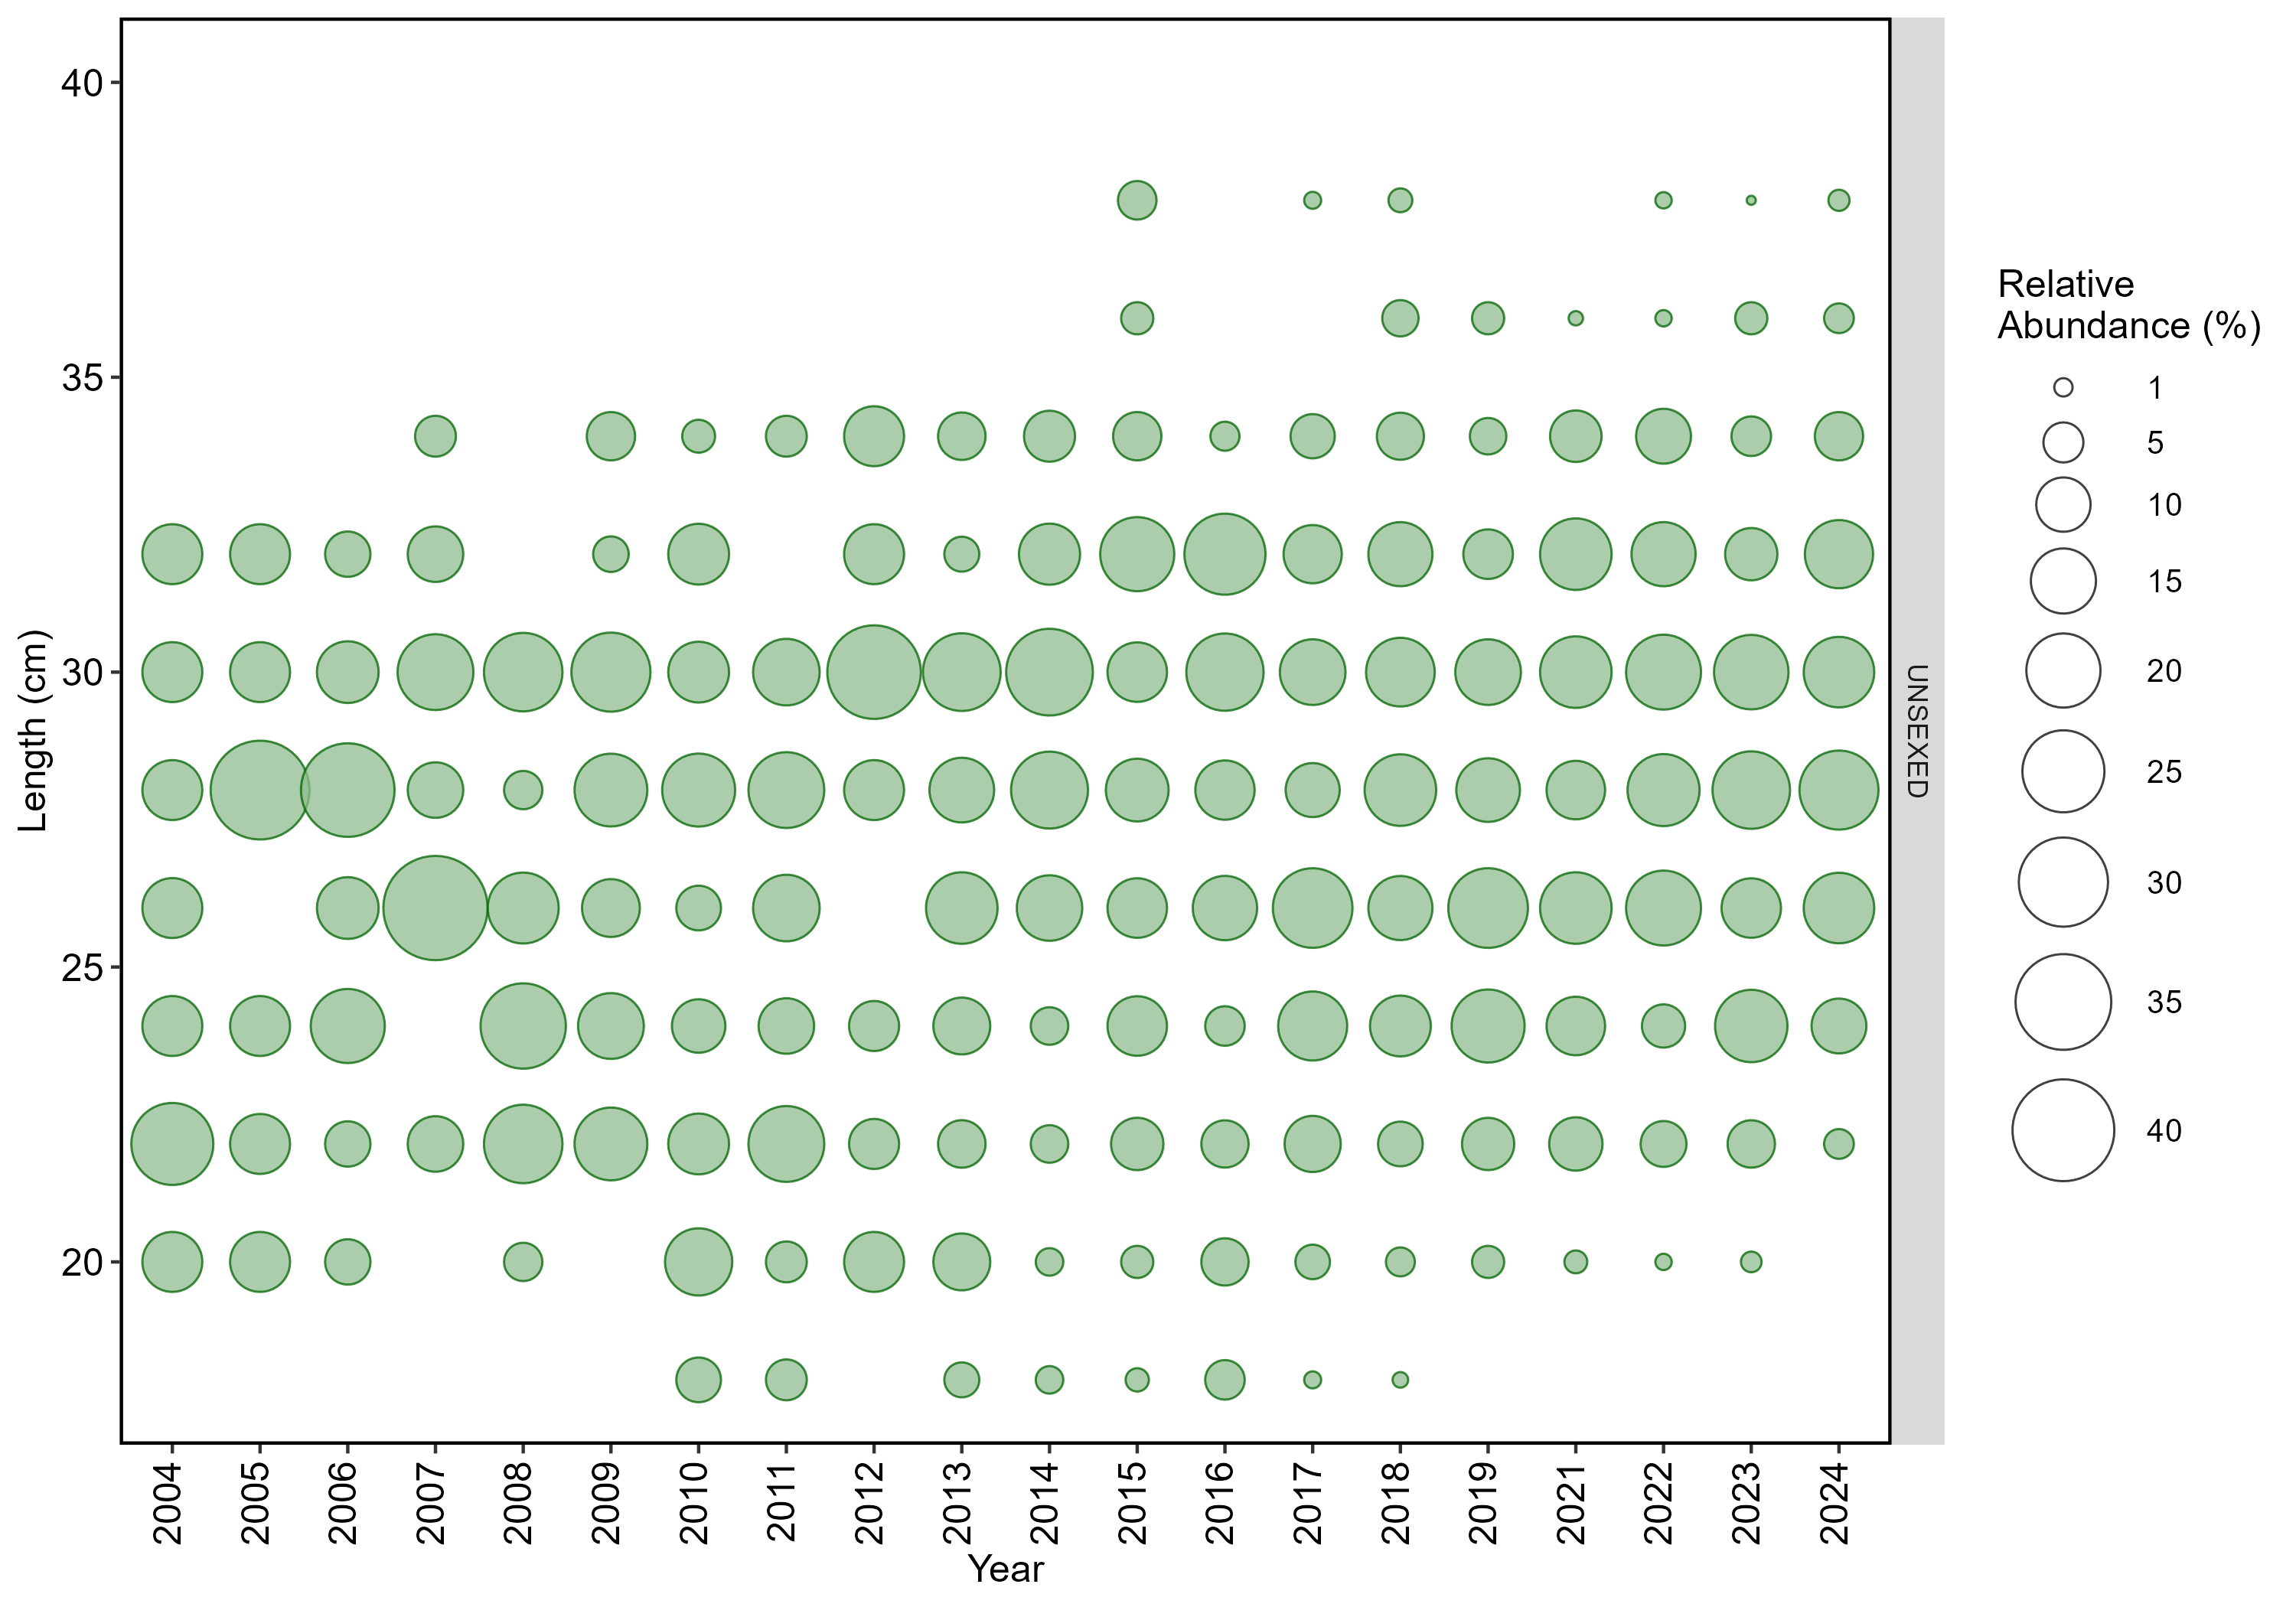
\includegraphics[width=0.95\linewidth,height=\textheight,keepaspectratio]{../plots/hkl_comps/plots/greenstriped rockfish_nwfsc_hkl_length_frequency_sex_0.png}

}

\caption{Length (cm) compostion data from the NWFSC HKLS for
greenstriped rockfish. Size of the circles within a year indicate higher
(larger circles) and lower (smaller circles) proportion observed by
length bin.}

\end{figure}%

\newpage{}

\subsection{Kelp greenling}\label{kelp-greenling}

To date, no assessment or analysis has been conducted on kelp greenling.
Across available data, kelp greenling have been observed and sampled by
the NWFSC WCGBTS. The NWFSC WCGBTS observed kelp greenling on an average
of 3 tows per year. For this species, a total of 8 maturity samples have
been collected coastwide (regardless of stock area), with 8 read
maturities. ODFW scientists have conducted research looking at the
influences of hypoxia on the catch per unit effort for kelp greenling.

\begingroup\fontsize{10}{12}\selectfont
\begingroup\fontsize{10}{12}\selectfont

\begin{longtable}[t]{>{\raggedleft\arraybackslash}p{2cm}>{\raggedleft\arraybackslash}p{3.5cm}>{\raggedleft\arraybackslash}p{2cm}>{\raggedleft\arraybackslash}p{2cm}>{\raggedleft\arraybackslash}p{2cm}}
\caption{\label{tab:unnamed-chunk-278}Total number of available lengths, read ages, and unread age structures by data source and
state for kelp greenling.}\\
\toprule
State & Source & Lengths & Ages & Age Structures\\
\midrule
\endfirsthead
\caption[]{Total number of available lengths, read ages, and unread age structures by data source and
state for kelp greenling. (\textit{continued)}}\\
\toprule
State & Source & Lengths & Ages & Age Structures\\
\midrule
\endhead

\endfoot
\bottomrule
\endlastfoot
WA & NWFSC WCGBTS & 217 & 0 & 197\\*
\end{longtable}
\endgroup{}
\endgroup{}

\begin{figure}[H]

{\centering 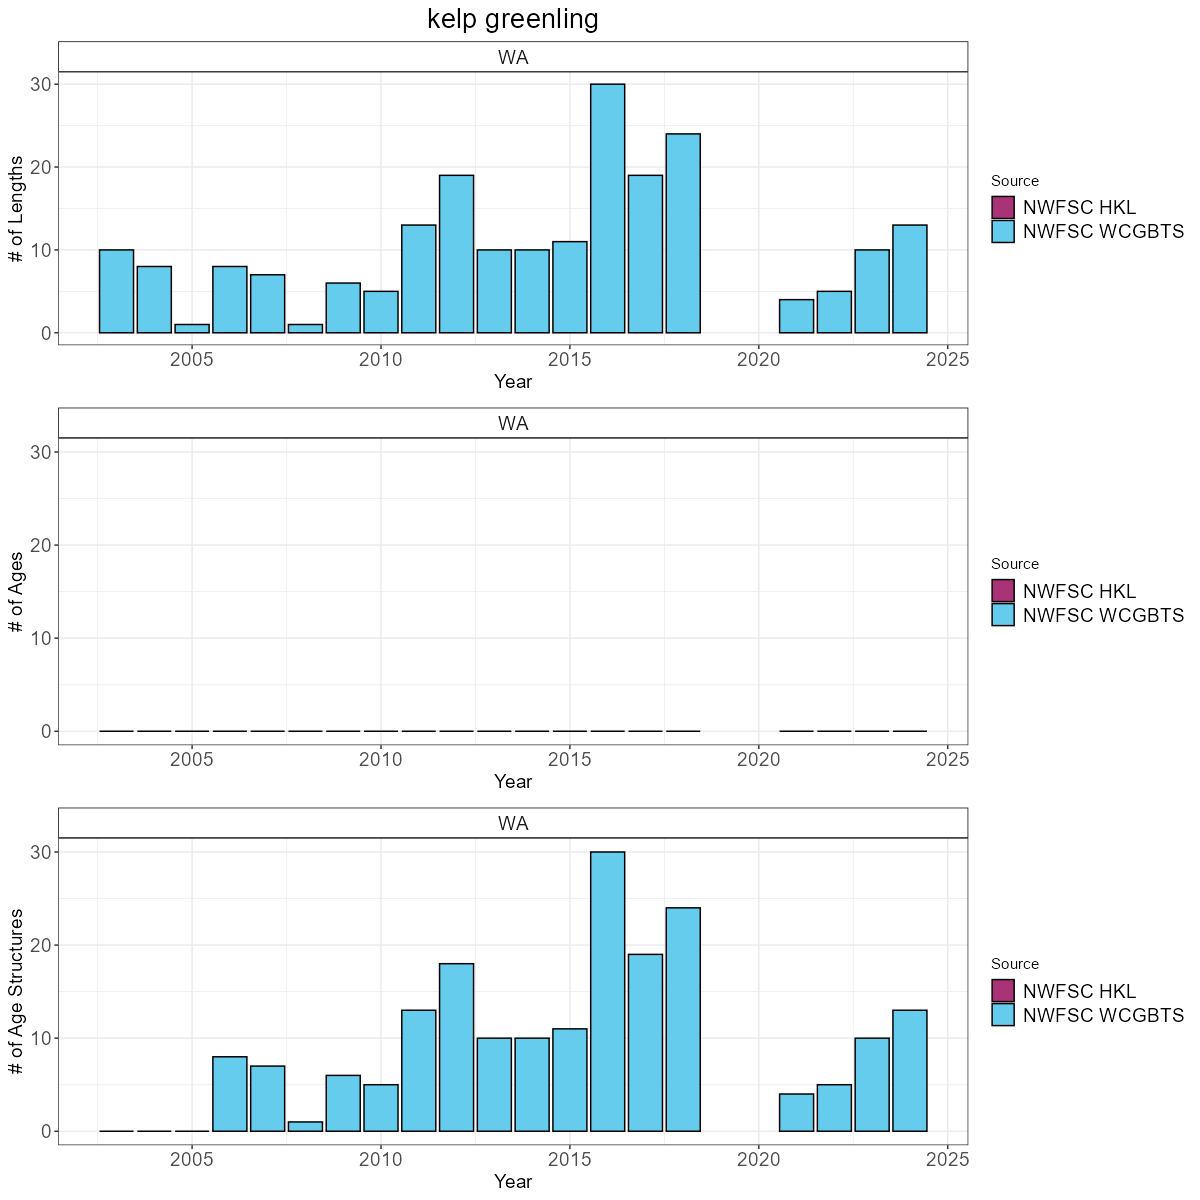
\includegraphics[width=0.95\linewidth,height=\textheight,keepaspectratio]{../plots/state_comparisons/kelp_greenling_state_compositions.png}

}

\caption{Total number of available lengths, read ages, and unread age
structures by data source by year for kelp greenling. Note the y-axis
maximum may differ by data type.}

\end{figure}%

\newpage{}

\subsection{Lingcod north}\label{lingcod-north}

The most recent assessment of lingcod north was a benchmark assessment
conducted in 2021. Across available data, lingcod north have been
observed and sampled by the NWFSC WCGBTS. The NWFSC WCGBTS observed
lingcod north on an average of 130 tows per year. For this species, a
total of 1161 maturity samples have been collected coastwide (regardless
of stock area), with 1031 read maturities. ODFW scientists have
conducted research looking at the influences of hypoxia on the catch per
unit effort for lingcod north.

\begingroup\fontsize{10}{12}\selectfont
\begingroup\fontsize{10}{12}\selectfont

\begin{longtable}[t]{>{\raggedleft\arraybackslash}p{2cm}>{\raggedleft\arraybackslash}p{3.5cm}>{\raggedleft\arraybackslash}p{2cm}>{\raggedleft\arraybackslash}p{2cm}>{\raggedleft\arraybackslash}p{2cm}}
\caption{\label{tab:unnamed-chunk-295}Total number of available lengths, read ages, and unread age structures by data source and
state for lingcod north.}\\
\toprule
State & Source & Lengths & Ages & Age Structures\\
\midrule
\endfirsthead
\caption[]{Total number of available lengths, read ages, and unread age structures by data source and
state for lingcod north. (\textit{continued)}}\\
\toprule
State & Source & Lengths & Ages & Age Structures\\
\midrule
\endhead

\endfoot
\bottomrule
\endlastfoot
CA & NWFSC WCGBTS & 2,582 & 780 & 632\\
OR & NWFSC WCGBTS & 9,992 & 2,782 & 2,721\\
WA & NWFSC WCGBTS & 7,151 & 1,582 & 1,513\\*
\end{longtable}
\endgroup{}
\endgroup{}

\begin{figure}[H]

{\centering 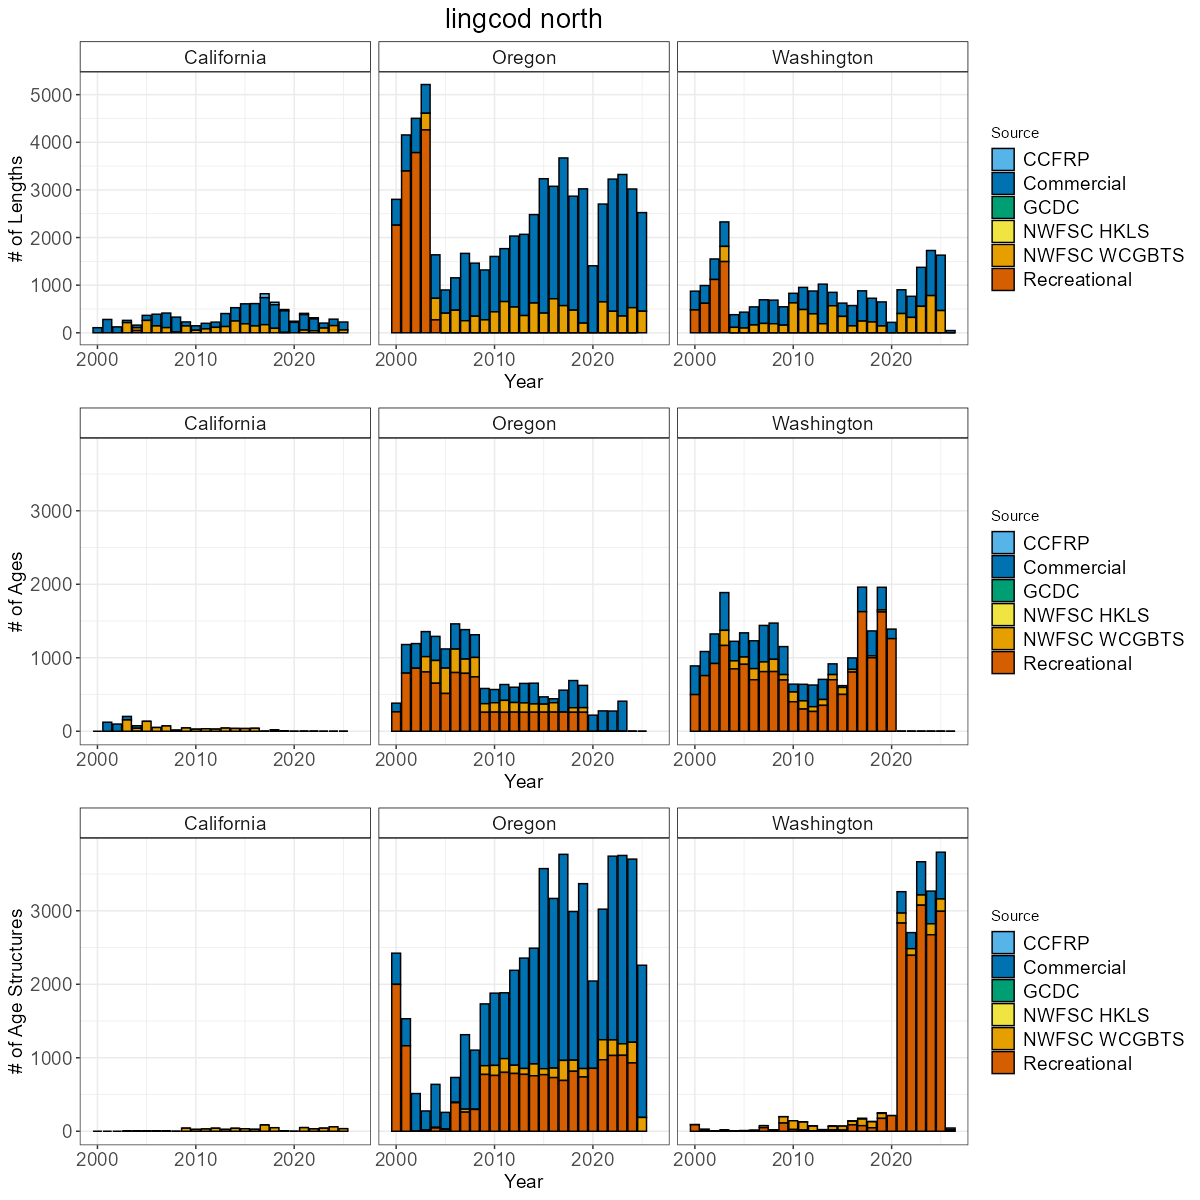
\includegraphics[width=0.95\linewidth,height=\textheight,keepaspectratio]{../plots/state_comparisons/lingcod_north_state_compositions.png}

}

\caption{Total number of available lengths, read ages, and unread age
structures by data source by year for lingcod north. Note the y-axis
maximum may differ by data type.}

\end{figure}%

\begin{figure}[H]

{\centering 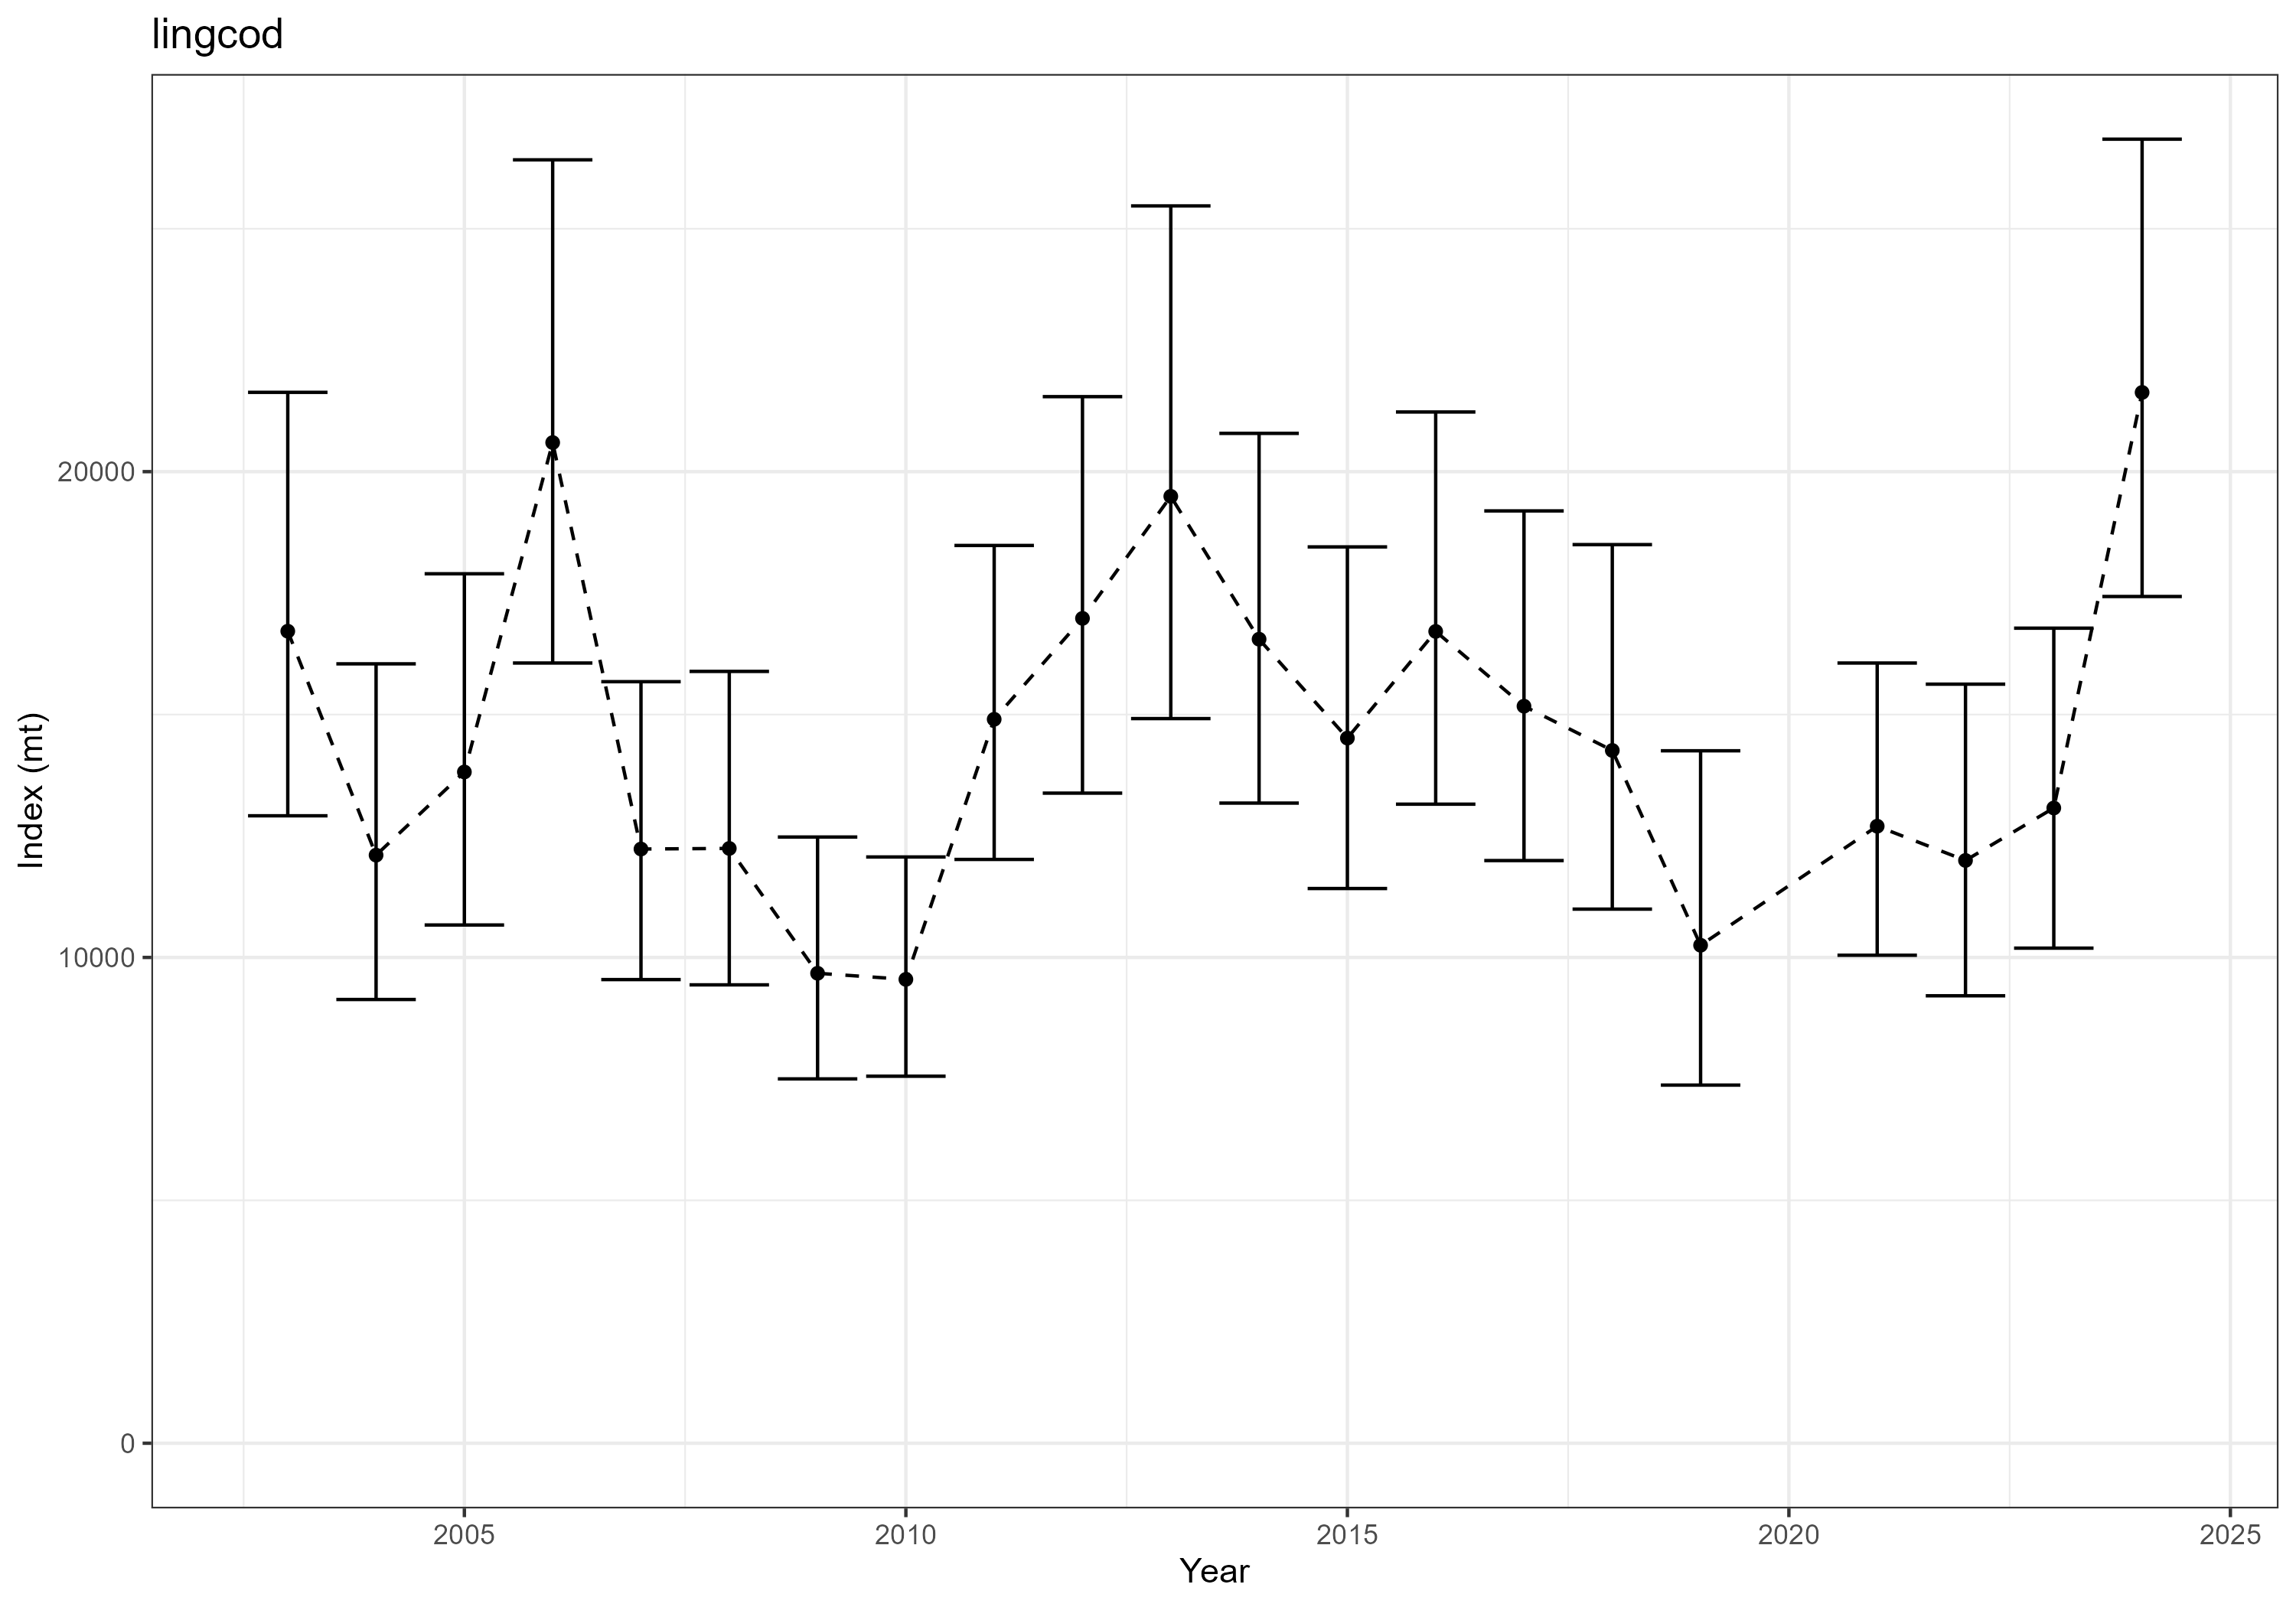
\includegraphics[width=0.95\linewidth,height=\textheight,keepaspectratio]{../plots/wcgbts_indices/lingcod_north_index.png}

}

\caption{Estimated relative index of abundance for lingcod north from
the NWFSC WCGBTS.}

\end{figure}%

\begin{figure}[H]

{\centering 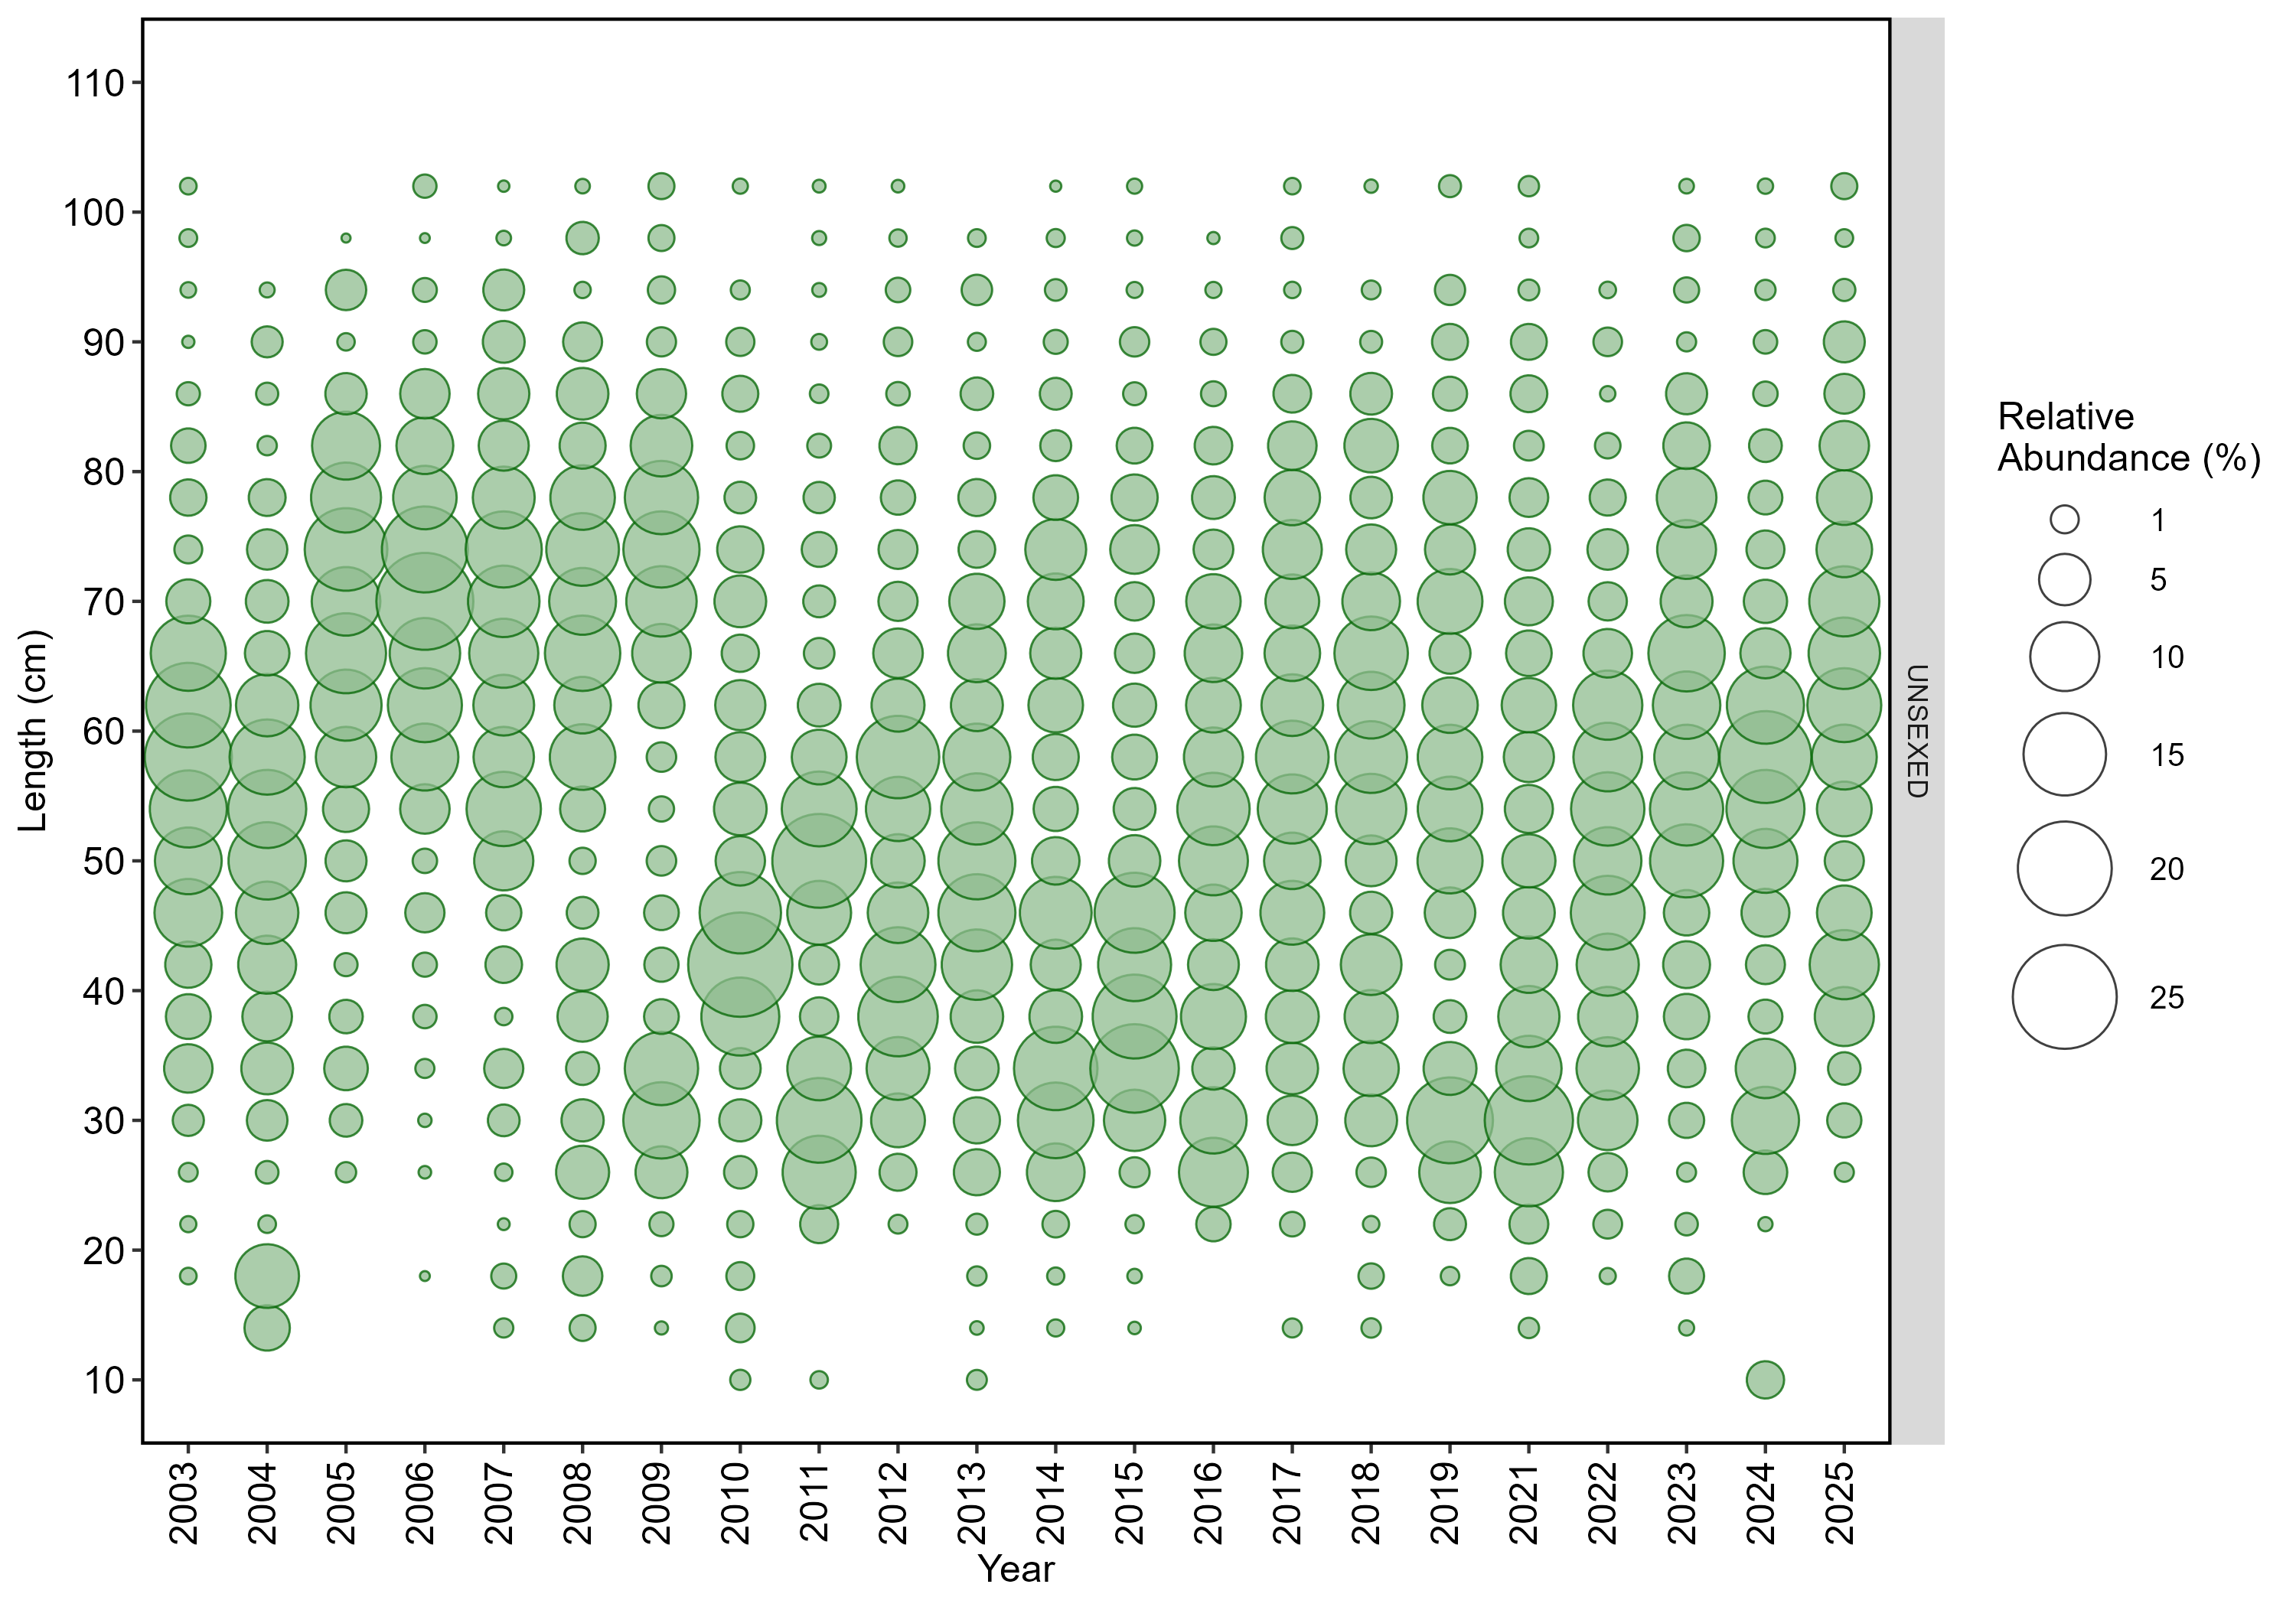
\includegraphics[width=0.95\linewidth,height=\textheight,keepaspectratio]{../plots/wcgbts_comps/plots/lingcod north_length_frequency_sex_0.png}

}

\caption{Length (cm) compostion data from the NWFSC WCGBTS for lingcod
north. Size of the circles within a year indicate higher (larger
circles) and lower (smaller circles) proportion observed by length bin.}

\end{figure}%

\newpage{}

\subsection{Lingcod south}\label{lingcod-south}

The most recent assessment of lingcod south was a benchmark assessment
conducted in 2021. Across available data, lingcod south have been
observed and sampled by both the NWFSC HKLS and WCGBTS. The NWFSC HKLS
observed lingcod south at an average of 26 sets per year. The NWFSC
WCGBTS observed lingcod south on an average of 79 tows per year. For
this species, a total of 1161 maturity samples have been collected
coastwide (regardless of stock area), with 1031 read maturities.

\begingroup\fontsize{10}{12}\selectfont
\begingroup\fontsize{10}{12}\selectfont

\begin{longtable}[t]{>{\raggedleft\arraybackslash}p{2cm}>{\raggedleft\arraybackslash}p{3.5cm}>{\raggedleft\arraybackslash}p{2cm}>{\raggedleft\arraybackslash}p{2cm}>{\raggedleft\arraybackslash}p{2cm}}
\caption{\label{tab:unnamed-chunk-312}Total number of available lengths, read ages, and unread age structures by data source and
state for lingcod south.}\\
\toprule
State & Source & Lengths & Ages & Age Structures\\
\midrule
\endfirsthead
\caption[]{Total number of available lengths, read ages, and unread age structures by data source and
state for lingcod south. (\textit{continued)}}\\
\toprule
State & Source & Lengths & Ages & Age Structures\\
\midrule
\endhead

\endfoot
\bottomrule
\endlastfoot
CA & NWFSC HKLS & 955 & 185 & 25\\
CA & NWFSC WCGBTS & 12,375 & 3,887 & 2,797\\*
\end{longtable}
\endgroup{}
\endgroup{}

\begin{figure}[H]

{\centering 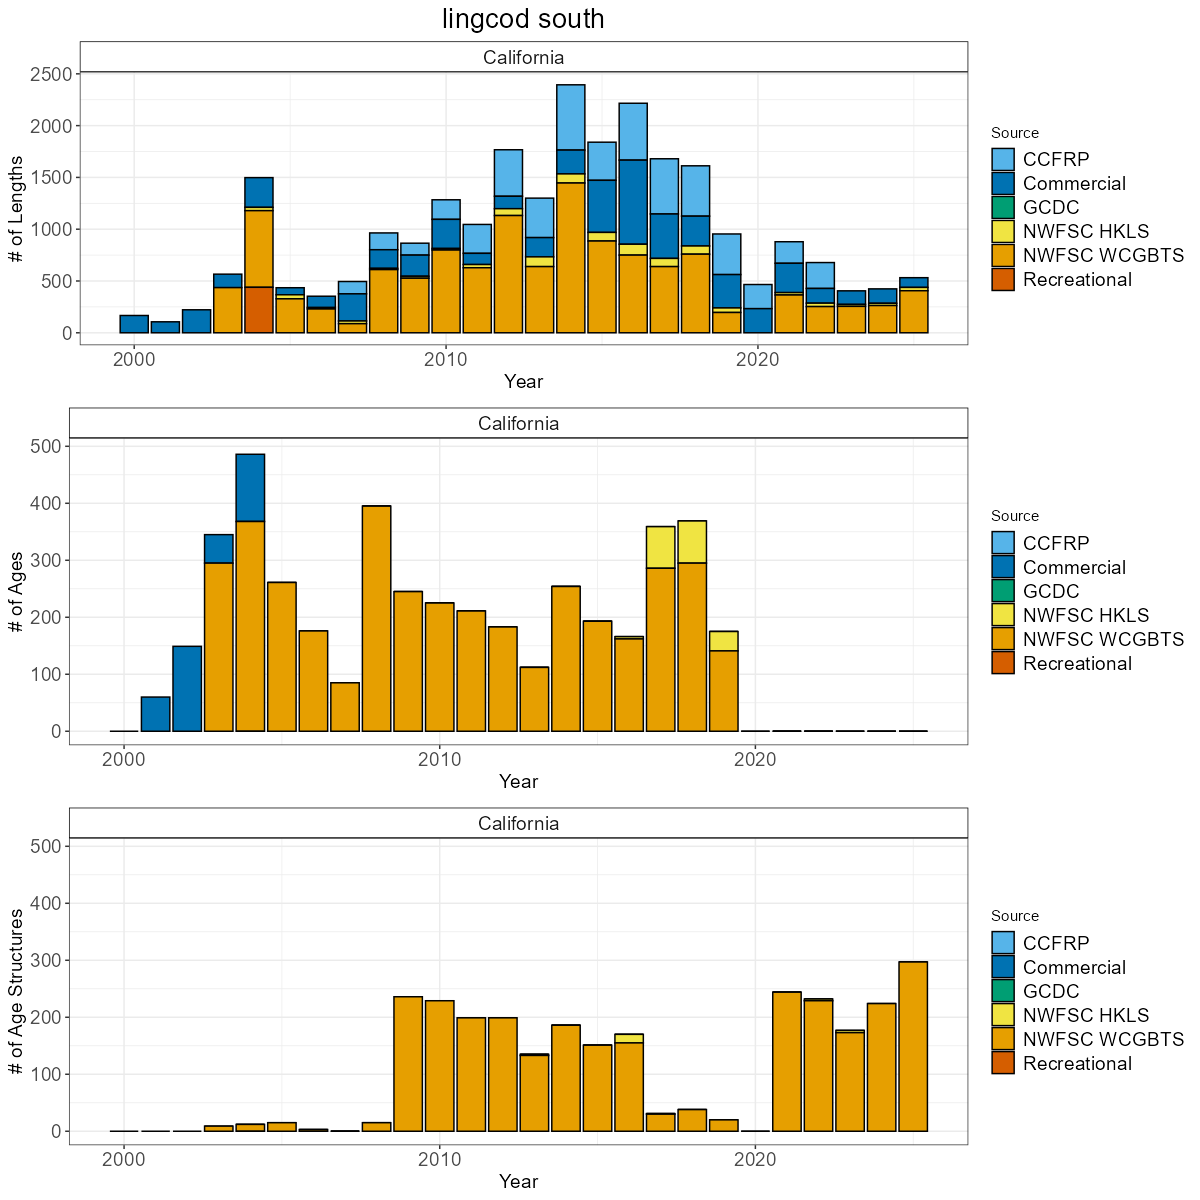
\includegraphics[width=0.95\linewidth,height=\textheight,keepaspectratio]{../plots/state_comparisons/lingcod_south_state_compositions.png}

}

\caption{Total number of available lengths, read ages, and unread age
structures by data source by year for lingcod south. Note the y-axis
maximum may differ by data type.}

\end{figure}%

\begin{figure}[H]

{\centering 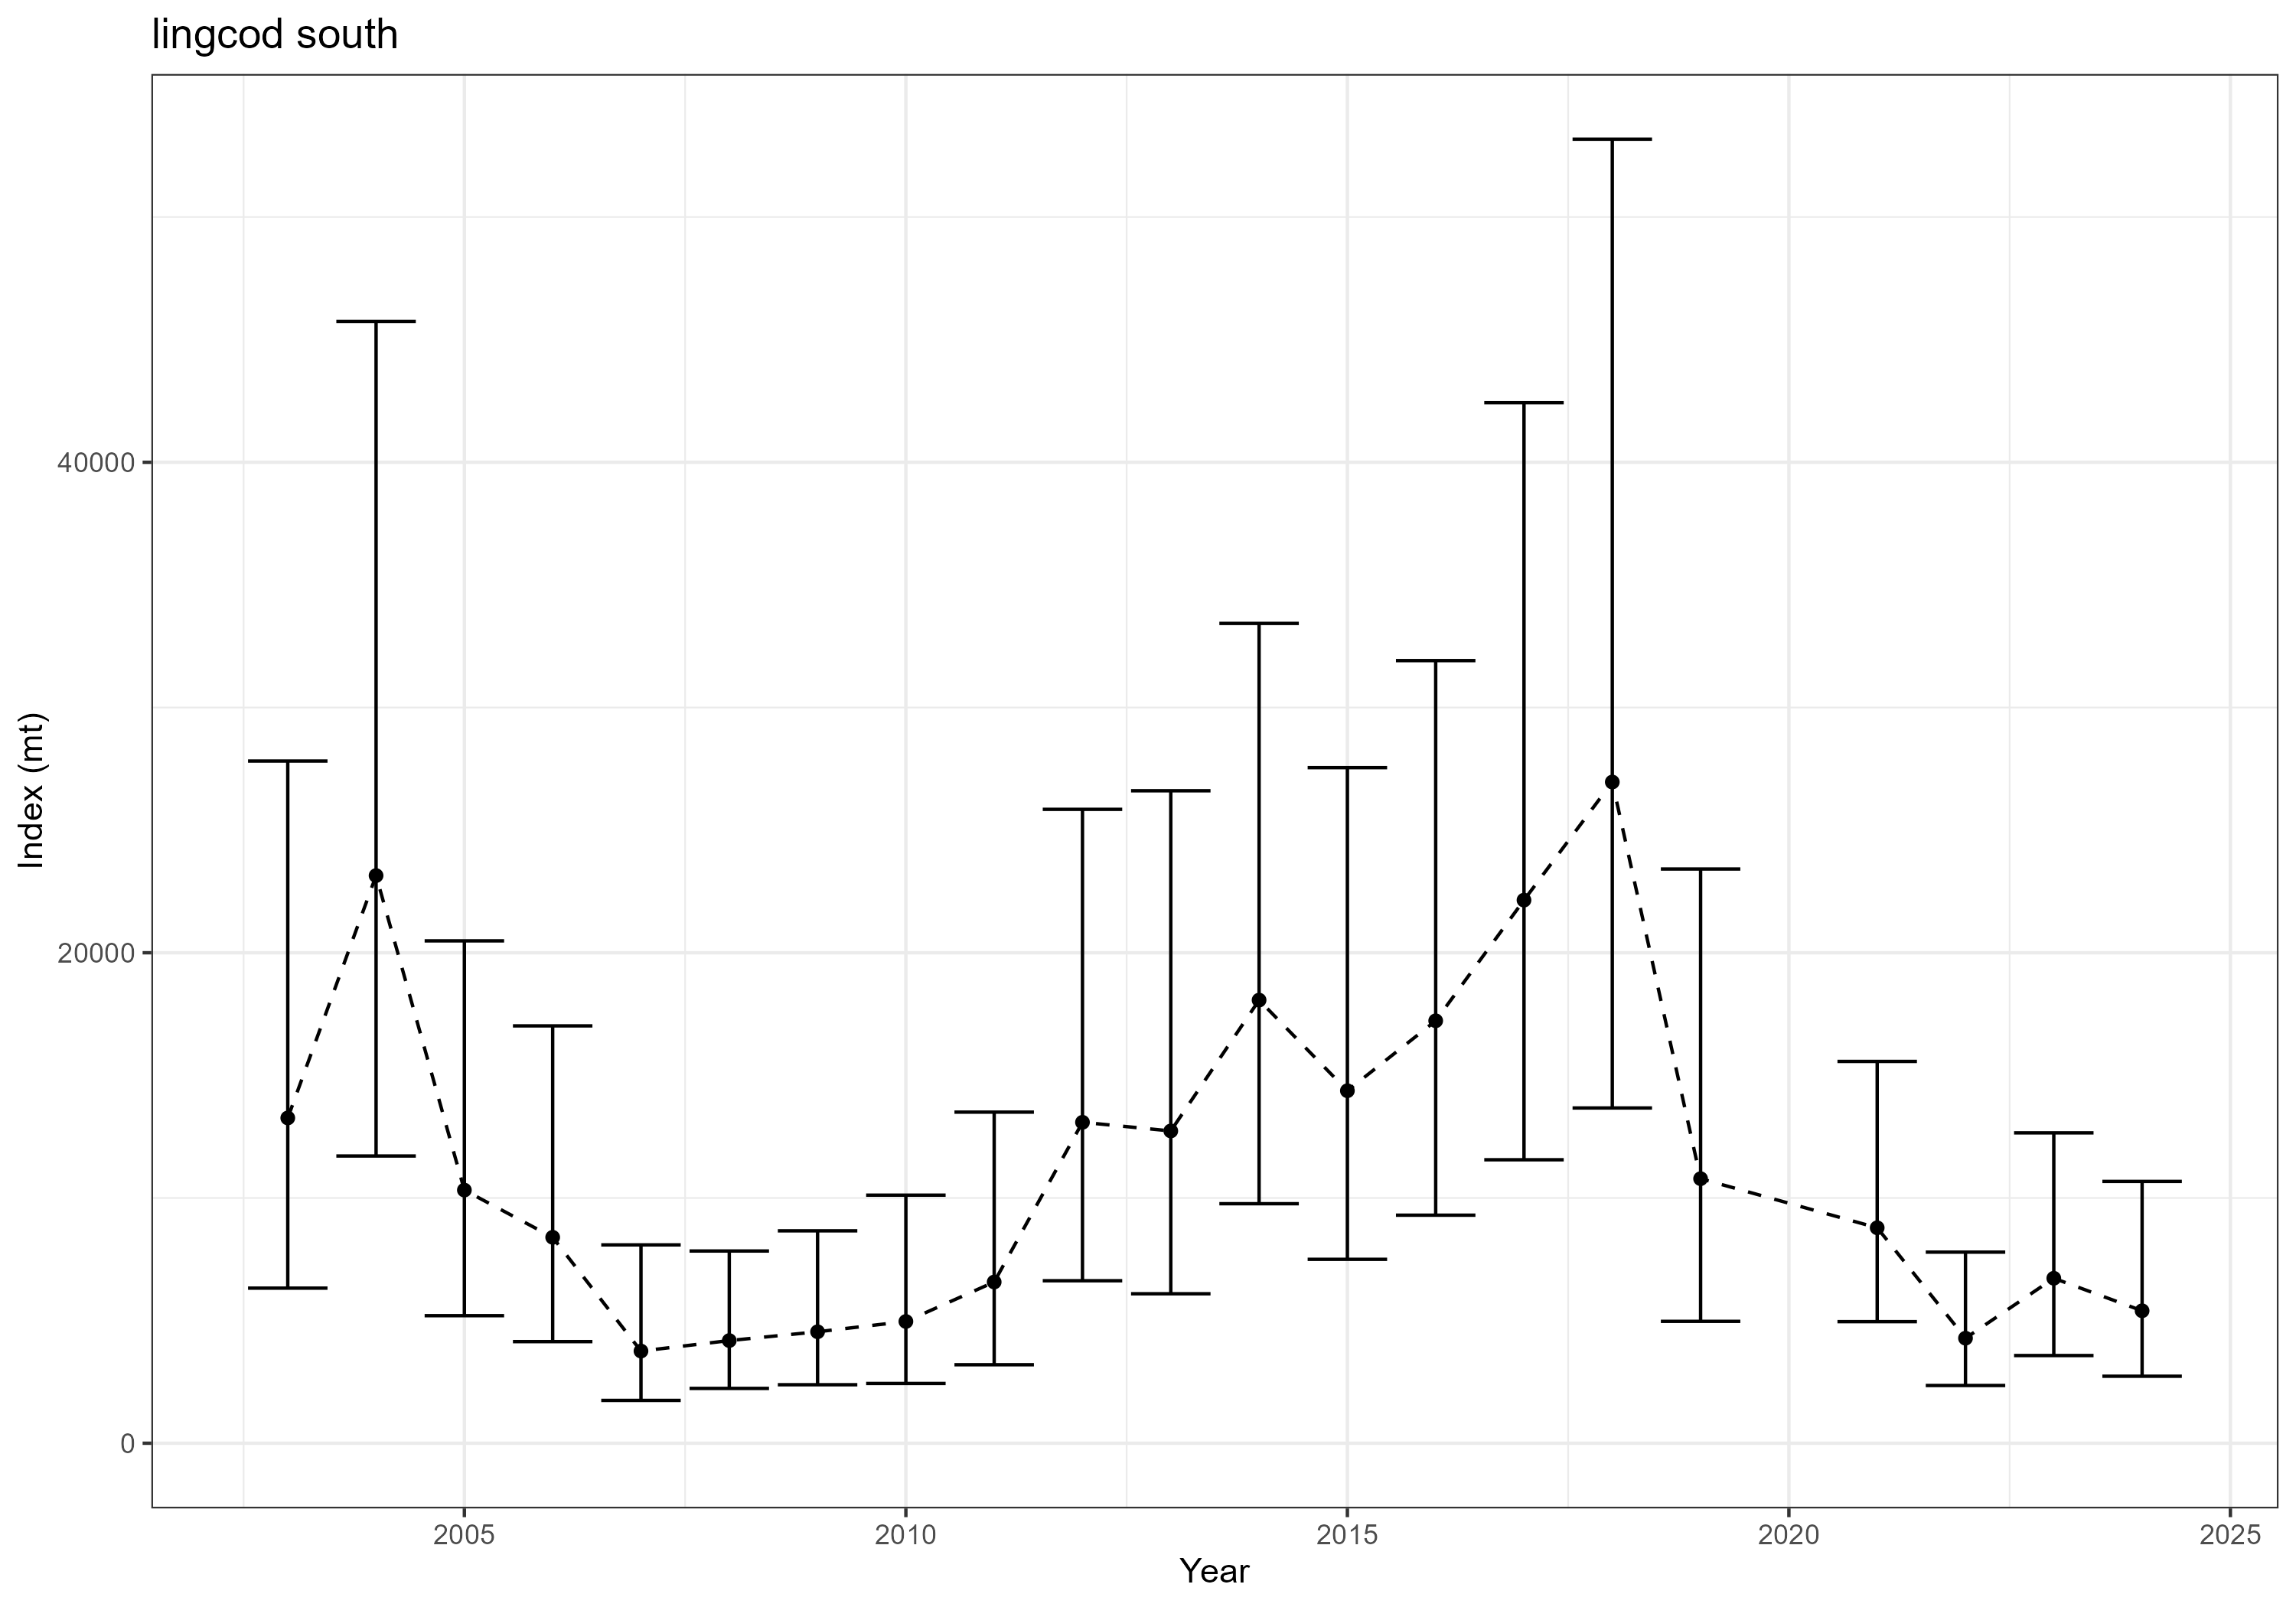
\includegraphics[width=0.95\linewidth,height=\textheight,keepaspectratio]{../plots/additional_wcgbts_indices/lingcod_south_index.png}

}

\caption{Estimated relative index of abundance for lingcod south from
the NWFSC WCGBTS.}

\end{figure}%

\begin{figure}[H]

{\centering 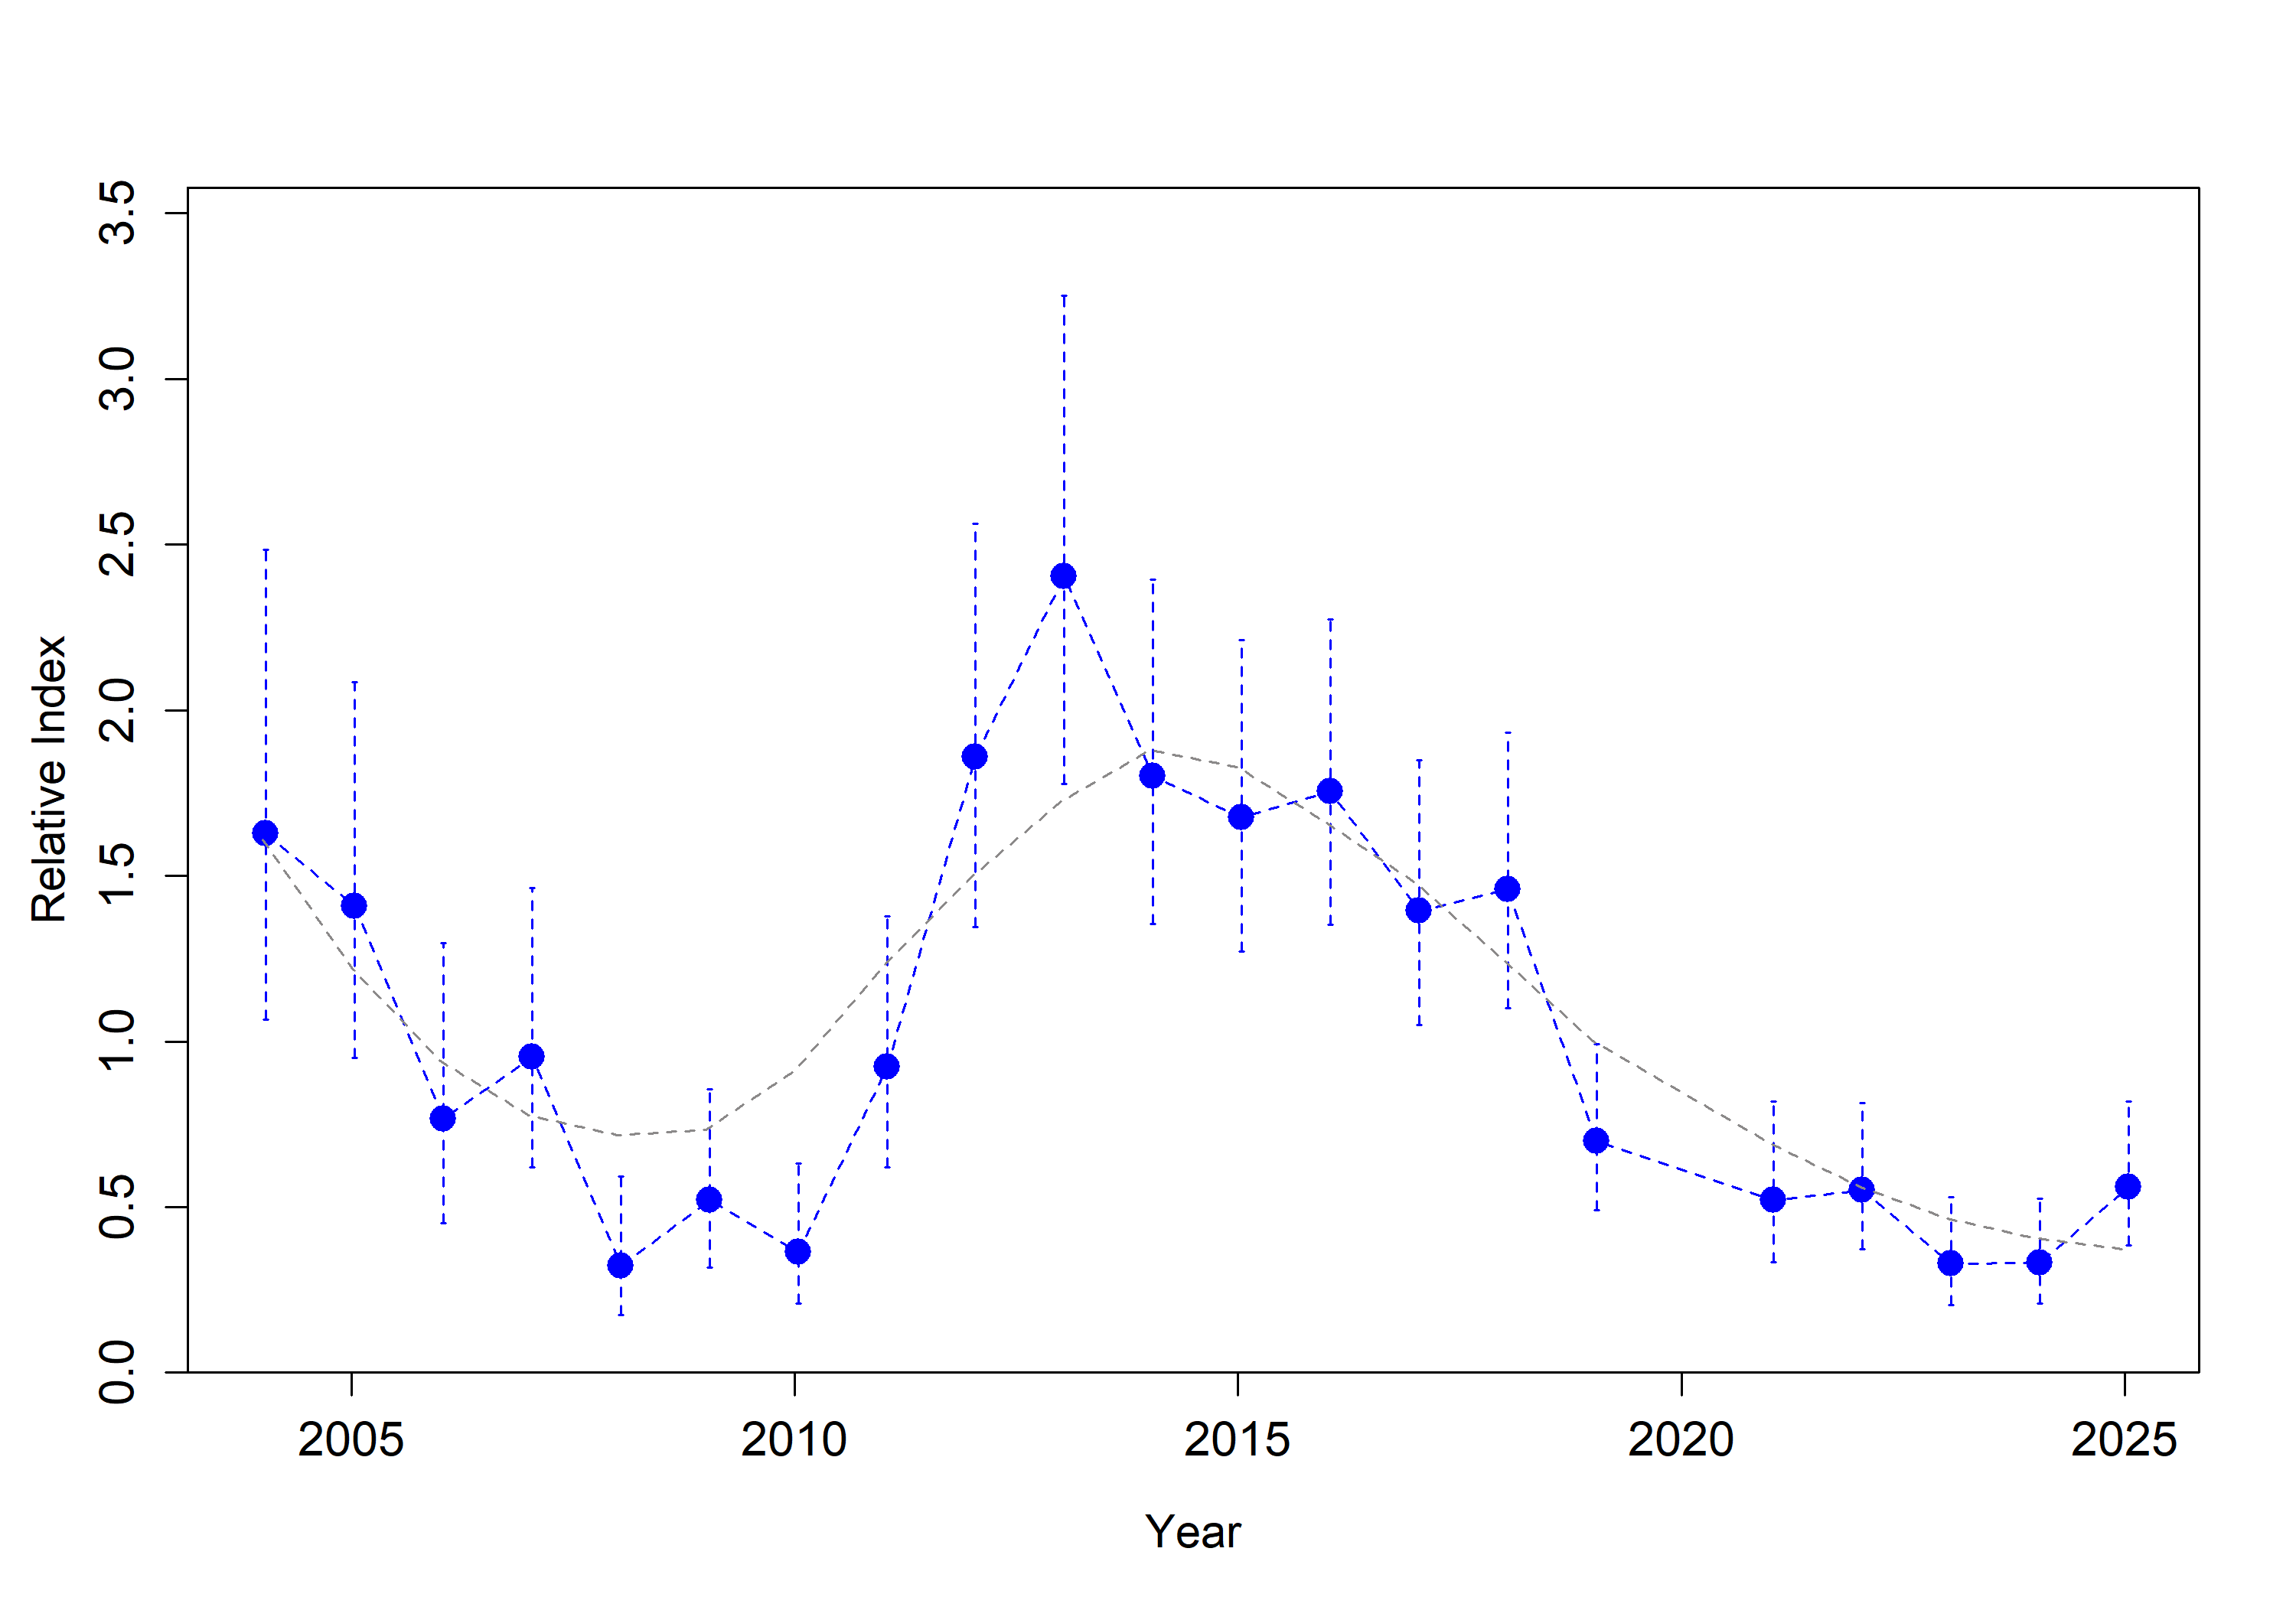
\includegraphics[width=0.95\linewidth,height=\textheight,keepaspectratio]{../plots/hkl_indices/lingcod south_negbinom index.png}

}

\caption{Estimated relative index of abundance for lingcod south from
the NWFSC HKLS.}

\end{figure}%

\begin{figure}[H]

{\centering 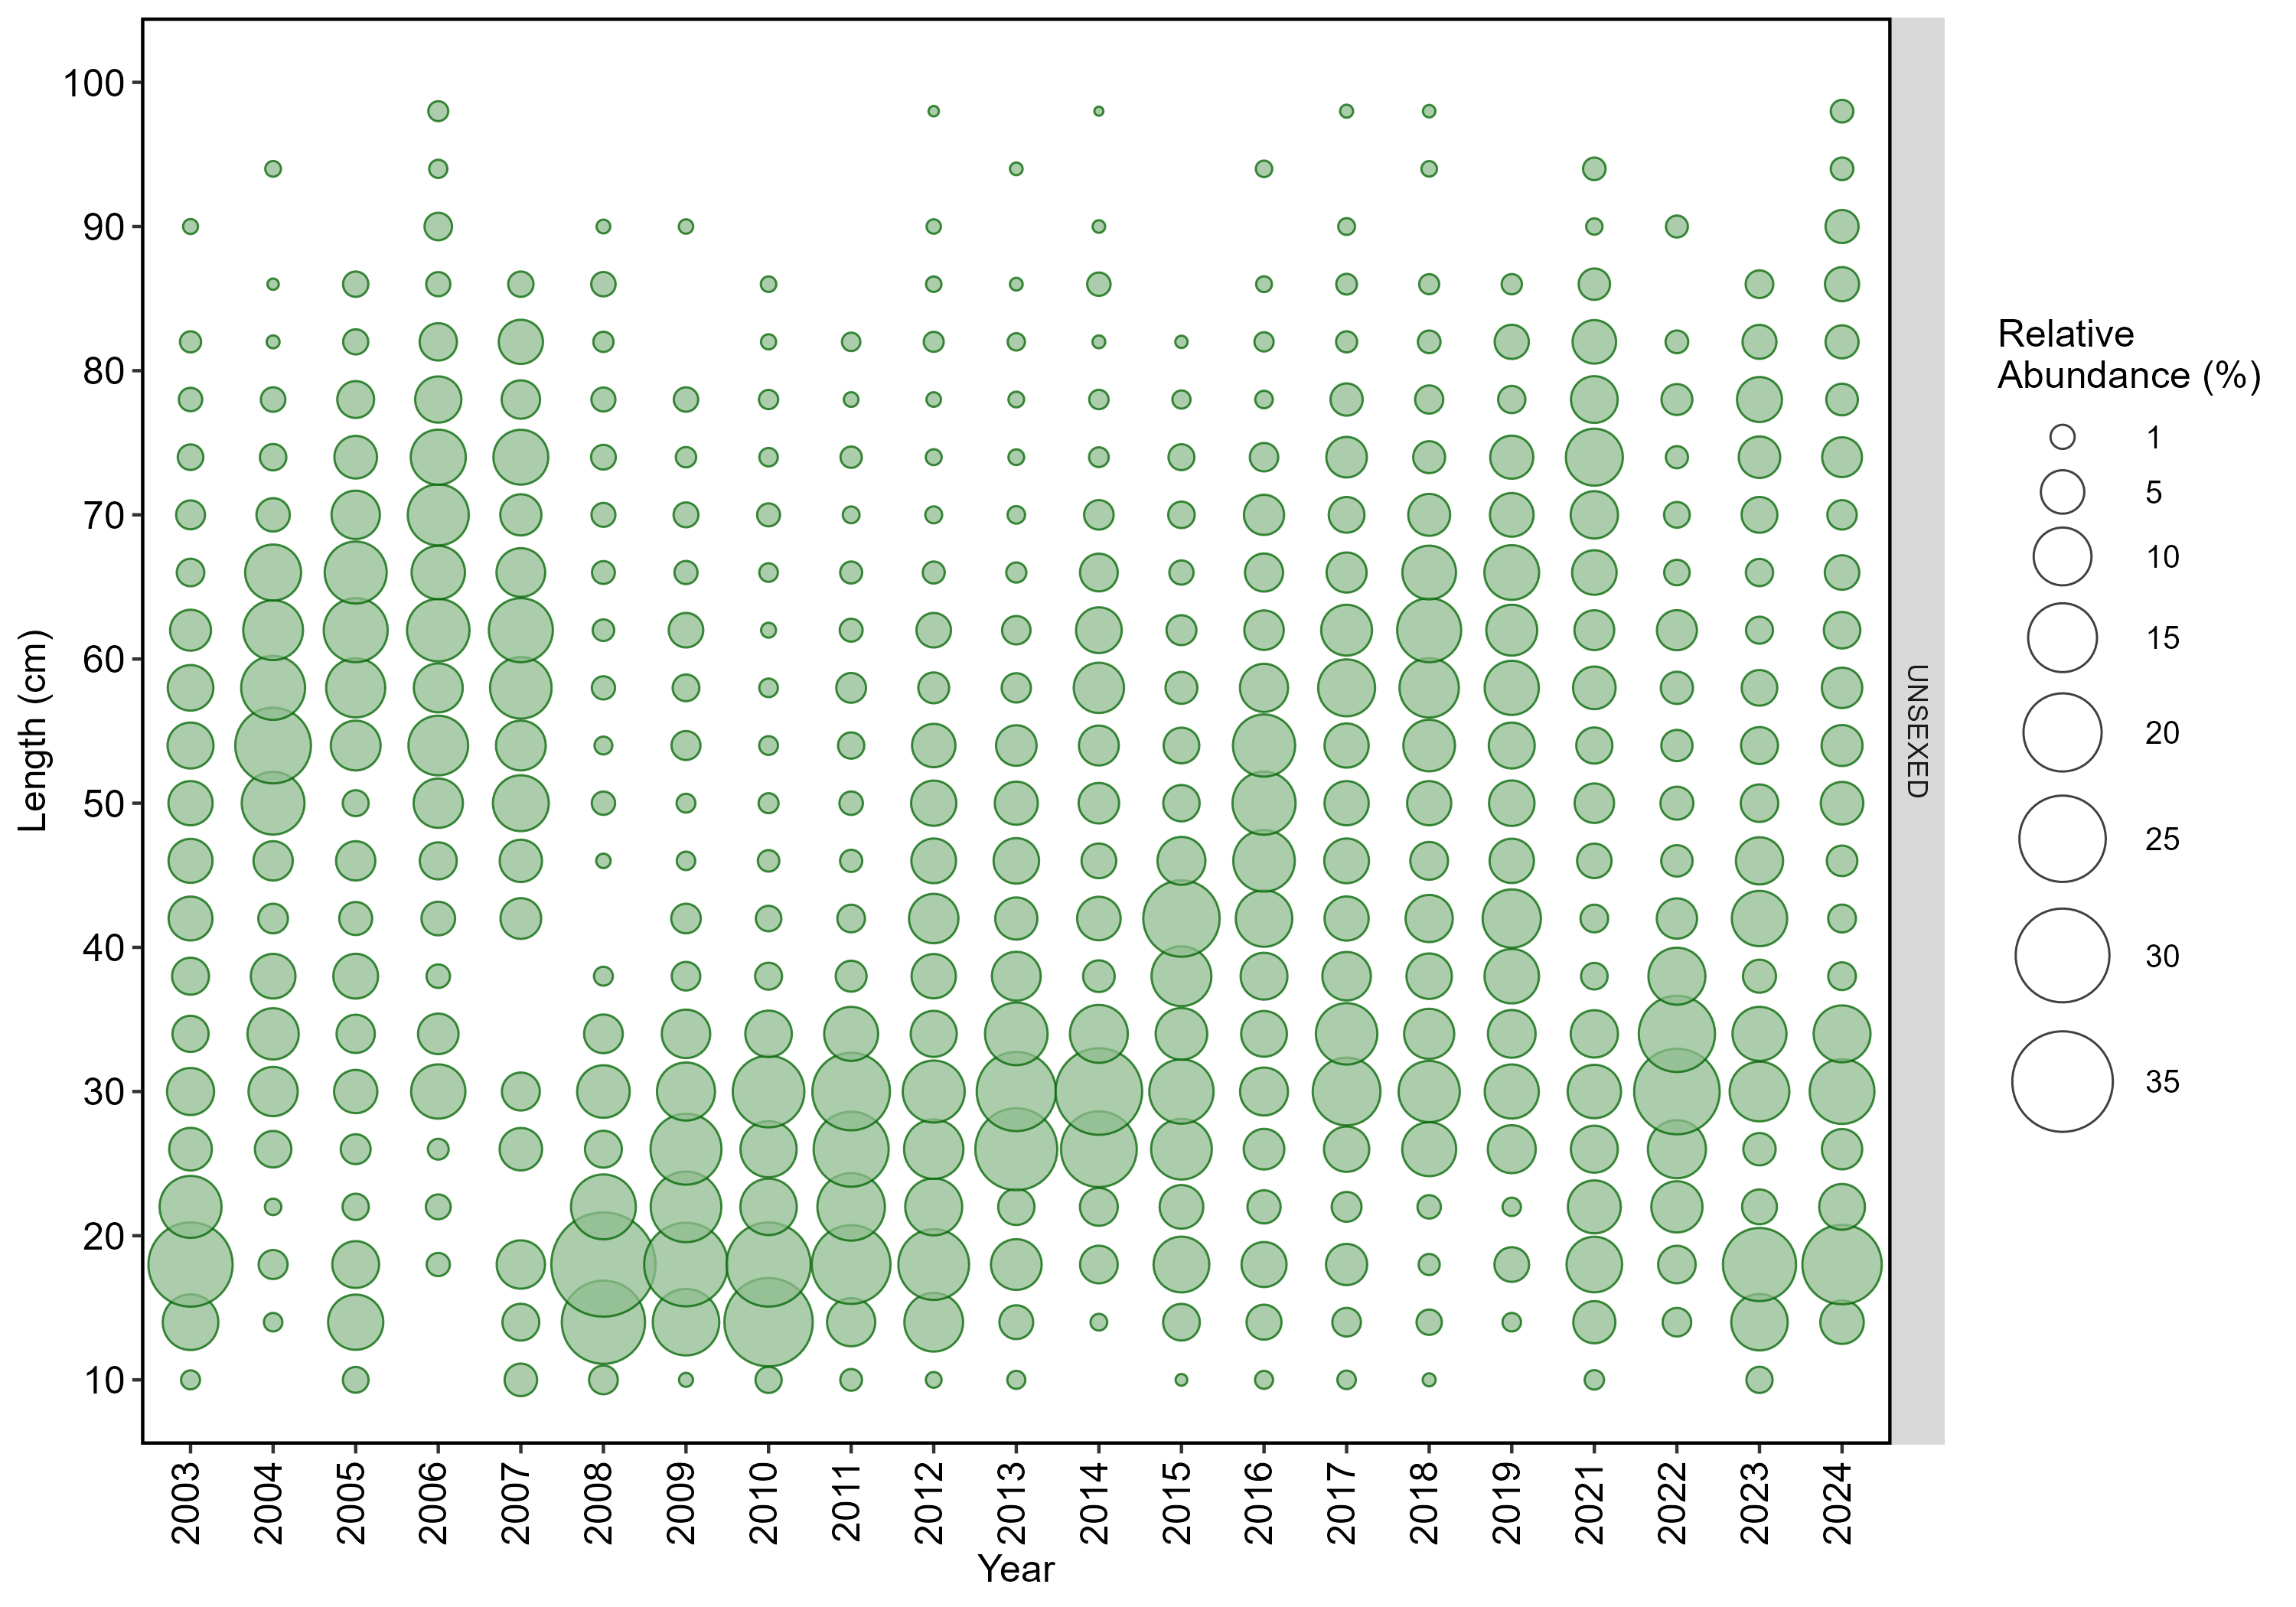
\includegraphics[width=0.95\linewidth,height=\textheight,keepaspectratio]{../plots/wcgbts_comps/plots/lingcod south_length_frequency_sex_0.png}

}

\caption{Length (cm) compostion data from the NWFSC WCGBTS for lingcod
south. Size of the circles within a year indicate higher (larger
circles) and lower (smaller circles) proportion observed by length bin.}

\end{figure}%

\begin{figure}[H]

{\centering 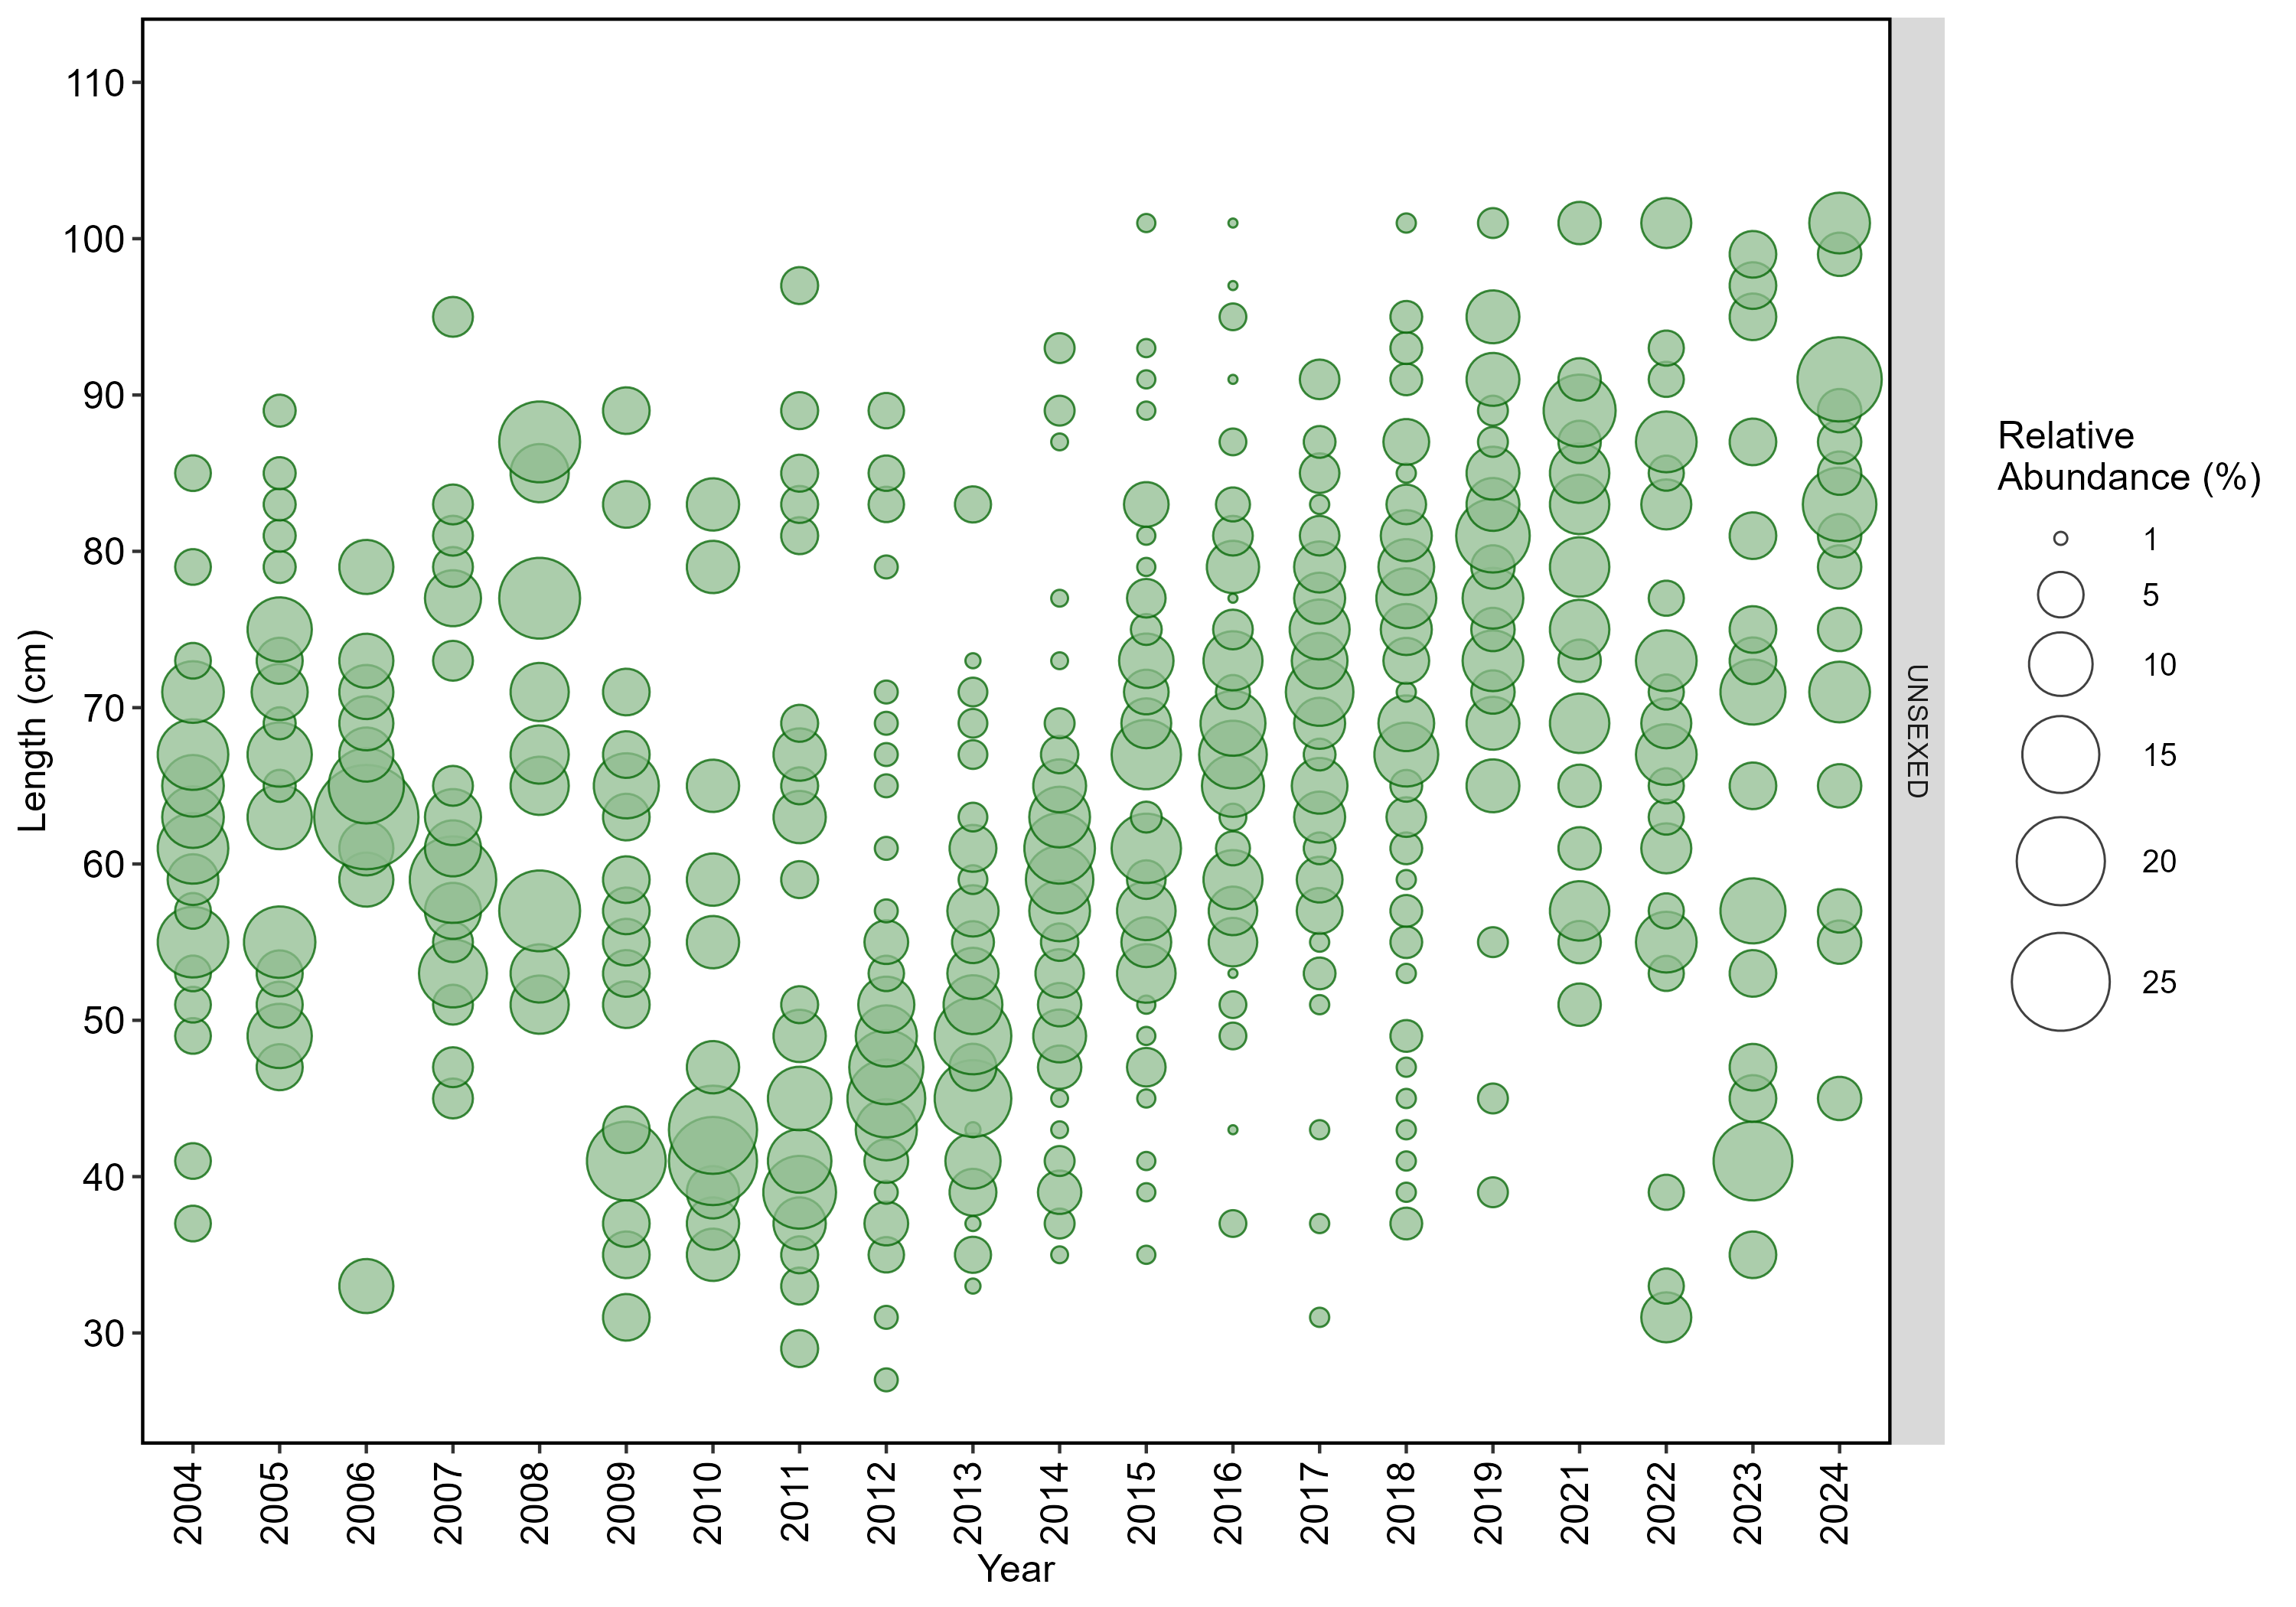
\includegraphics[width=0.95\linewidth,height=\textheight,keepaspectratio]{../plots/hkl_comps/plots/lingcod south_nwfsc_hkl_length_frequency_sex_0.png}

}

\caption{Length (cm) compostion data from the NWFSC HKLS for lingcod
south. Size of the circles within a year indicate higher (larger
circles) and lower (smaller circles) proportion observed by length bin.}

\end{figure}%

\newpage{}

\subsection{Longnose skate}\label{longnose-skate}

The most recent assessment of longnose skate was a benchmark assessment
conducted in 2019. Across available data, longnose skate have been
observed and sampled by the NWFSC WCGBTS. The NWFSC WCGBTS observed
longnose skate on an average of 384 tows per year. For this species, a
total of 508 maturity samples have been collected coastwide (regardless
of stock area), with 508 read maturities.

\begingroup\fontsize{10}{12}\selectfont
\begingroup\fontsize{10}{12}\selectfont

\begin{longtable}[t]{>{\raggedleft\arraybackslash}p{2cm}>{\raggedleft\arraybackslash}p{3.5cm}>{\raggedleft\arraybackslash}p{2cm}>{\raggedleft\arraybackslash}p{2cm}>{\raggedleft\arraybackslash}p{2cm}}
\caption{\label{tab:unnamed-chunk-329}Total number of available lengths, read ages, and unread age structures by data source and
state for longnose skate.}\\
\toprule
State & Source & Lengths & Ages & Age Structures\\
\midrule
\endfirsthead
\caption[]{Total number of available lengths, read ages, and unread age structures by data source and
state for longnose skate. (\textit{continued)}}\\
\toprule
State & Source & Lengths & Ages & Age Structures\\
\midrule
\endhead

\endfoot
\bottomrule
\endlastfoot
CA & NWFSC WCGBTS & 36,040 & 337 & 1,443\\
OR & NWFSC WCGBTS & 19,097 & 227 & 993\\
WA & NWFSC WCGBTS & 9,346 & 84 & 414\\*
\end{longtable}
\endgroup{}
\endgroup{}

\begin{figure}[H]

{\centering 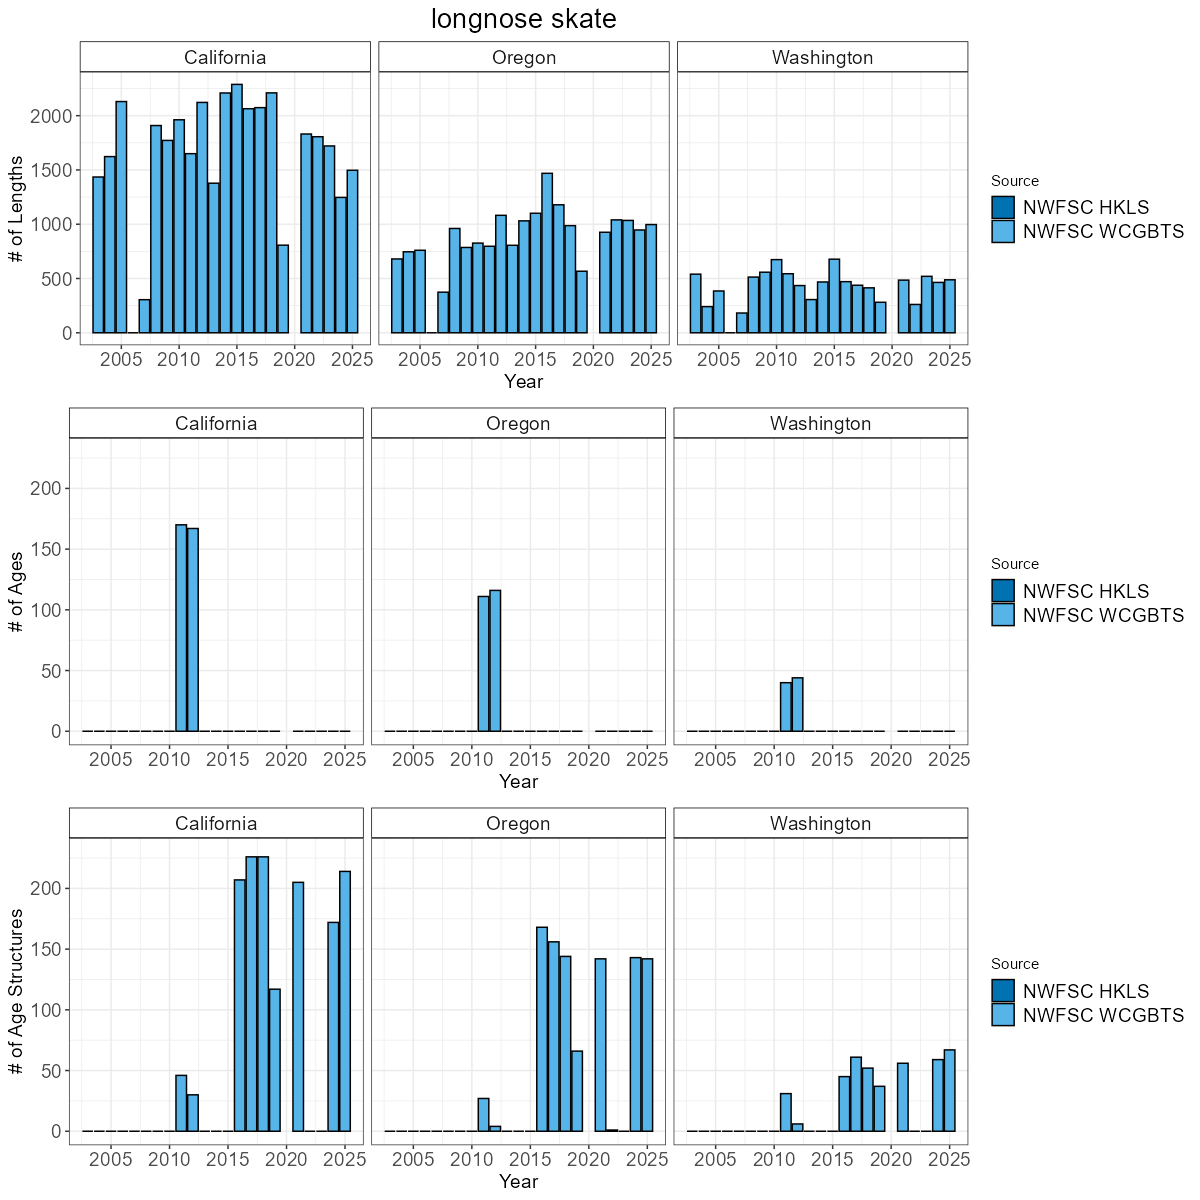
\includegraphics[width=0.95\linewidth,height=\textheight,keepaspectratio]{../plots/state_comparisons/longnose_skate_state_compositions.png}

}

\caption{Total number of available lengths, read ages, and unread age
structures by data source by year for longnose skate. Note the y-axis
maximum may differ by data type.}

\end{figure}%

\begin{figure}[H]

{\centering 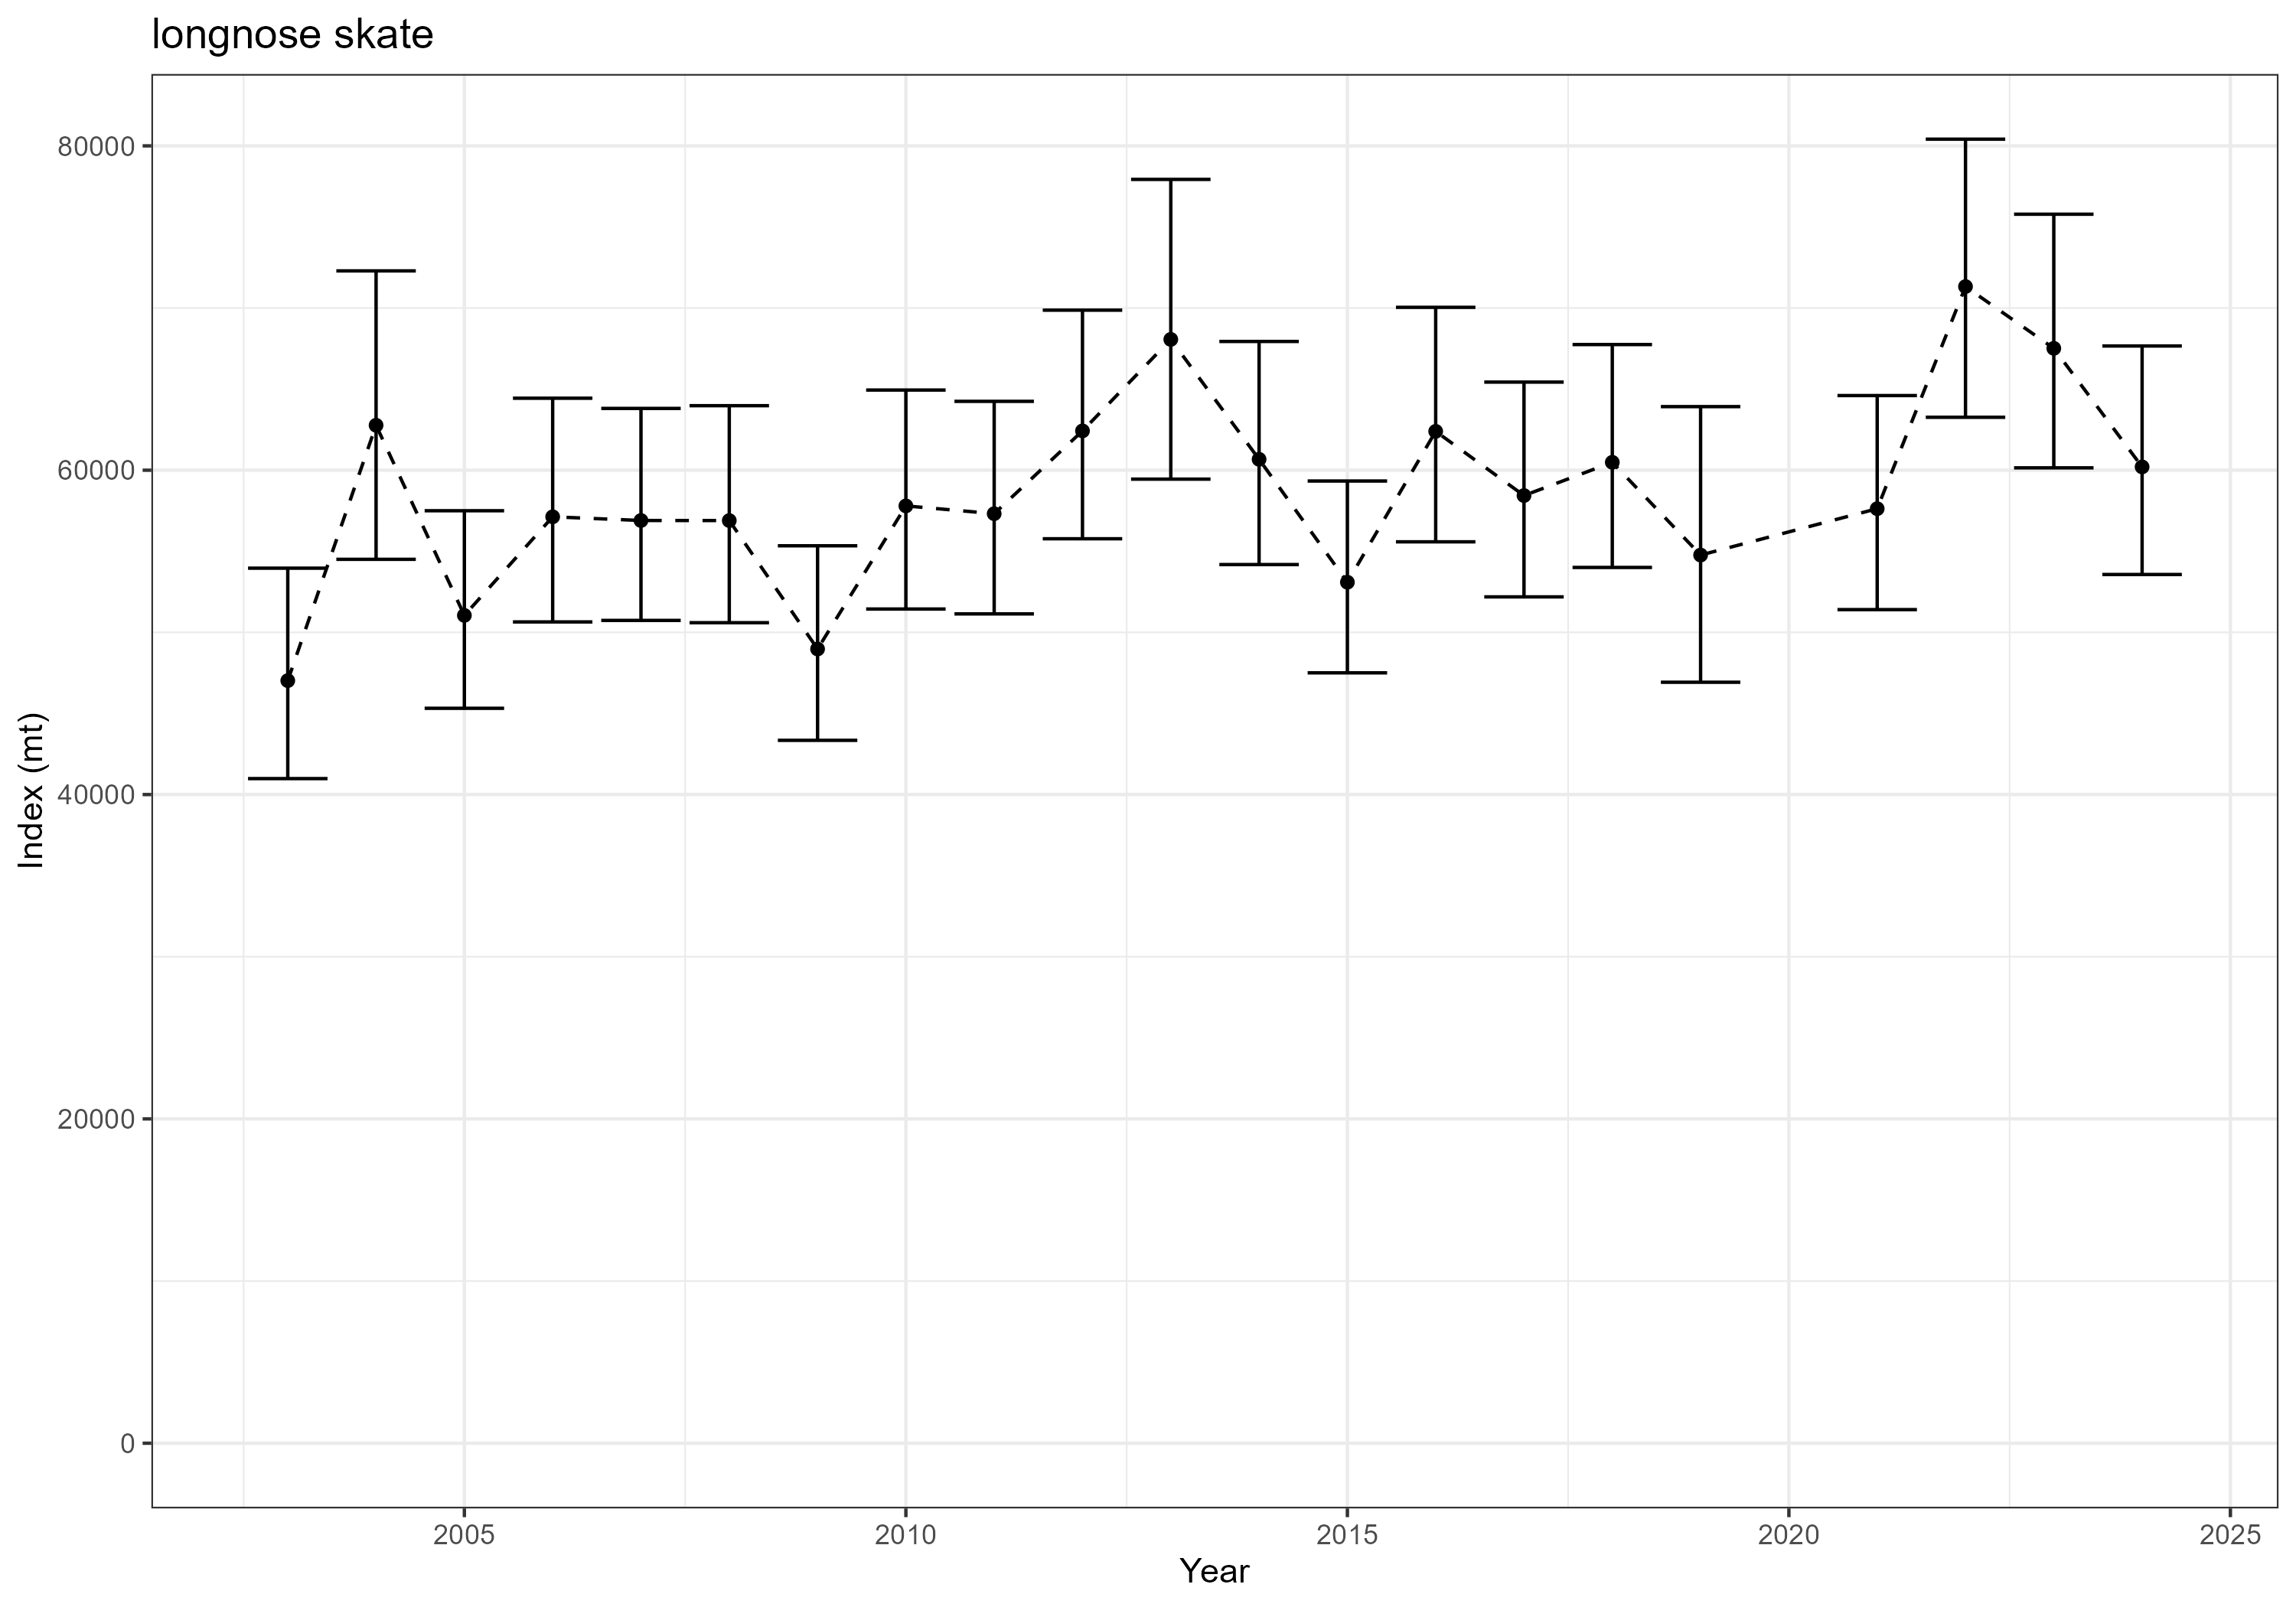
\includegraphics[width=0.95\linewidth,height=\textheight,keepaspectratio]{../plots/wcgbts_indices/longnose_skate_index.png}

}

\caption{Estimated relative index of abundance for longnose skate from
the NWFSC WCGBTS.}

\end{figure}%

\begin{figure}[H]

{\centering 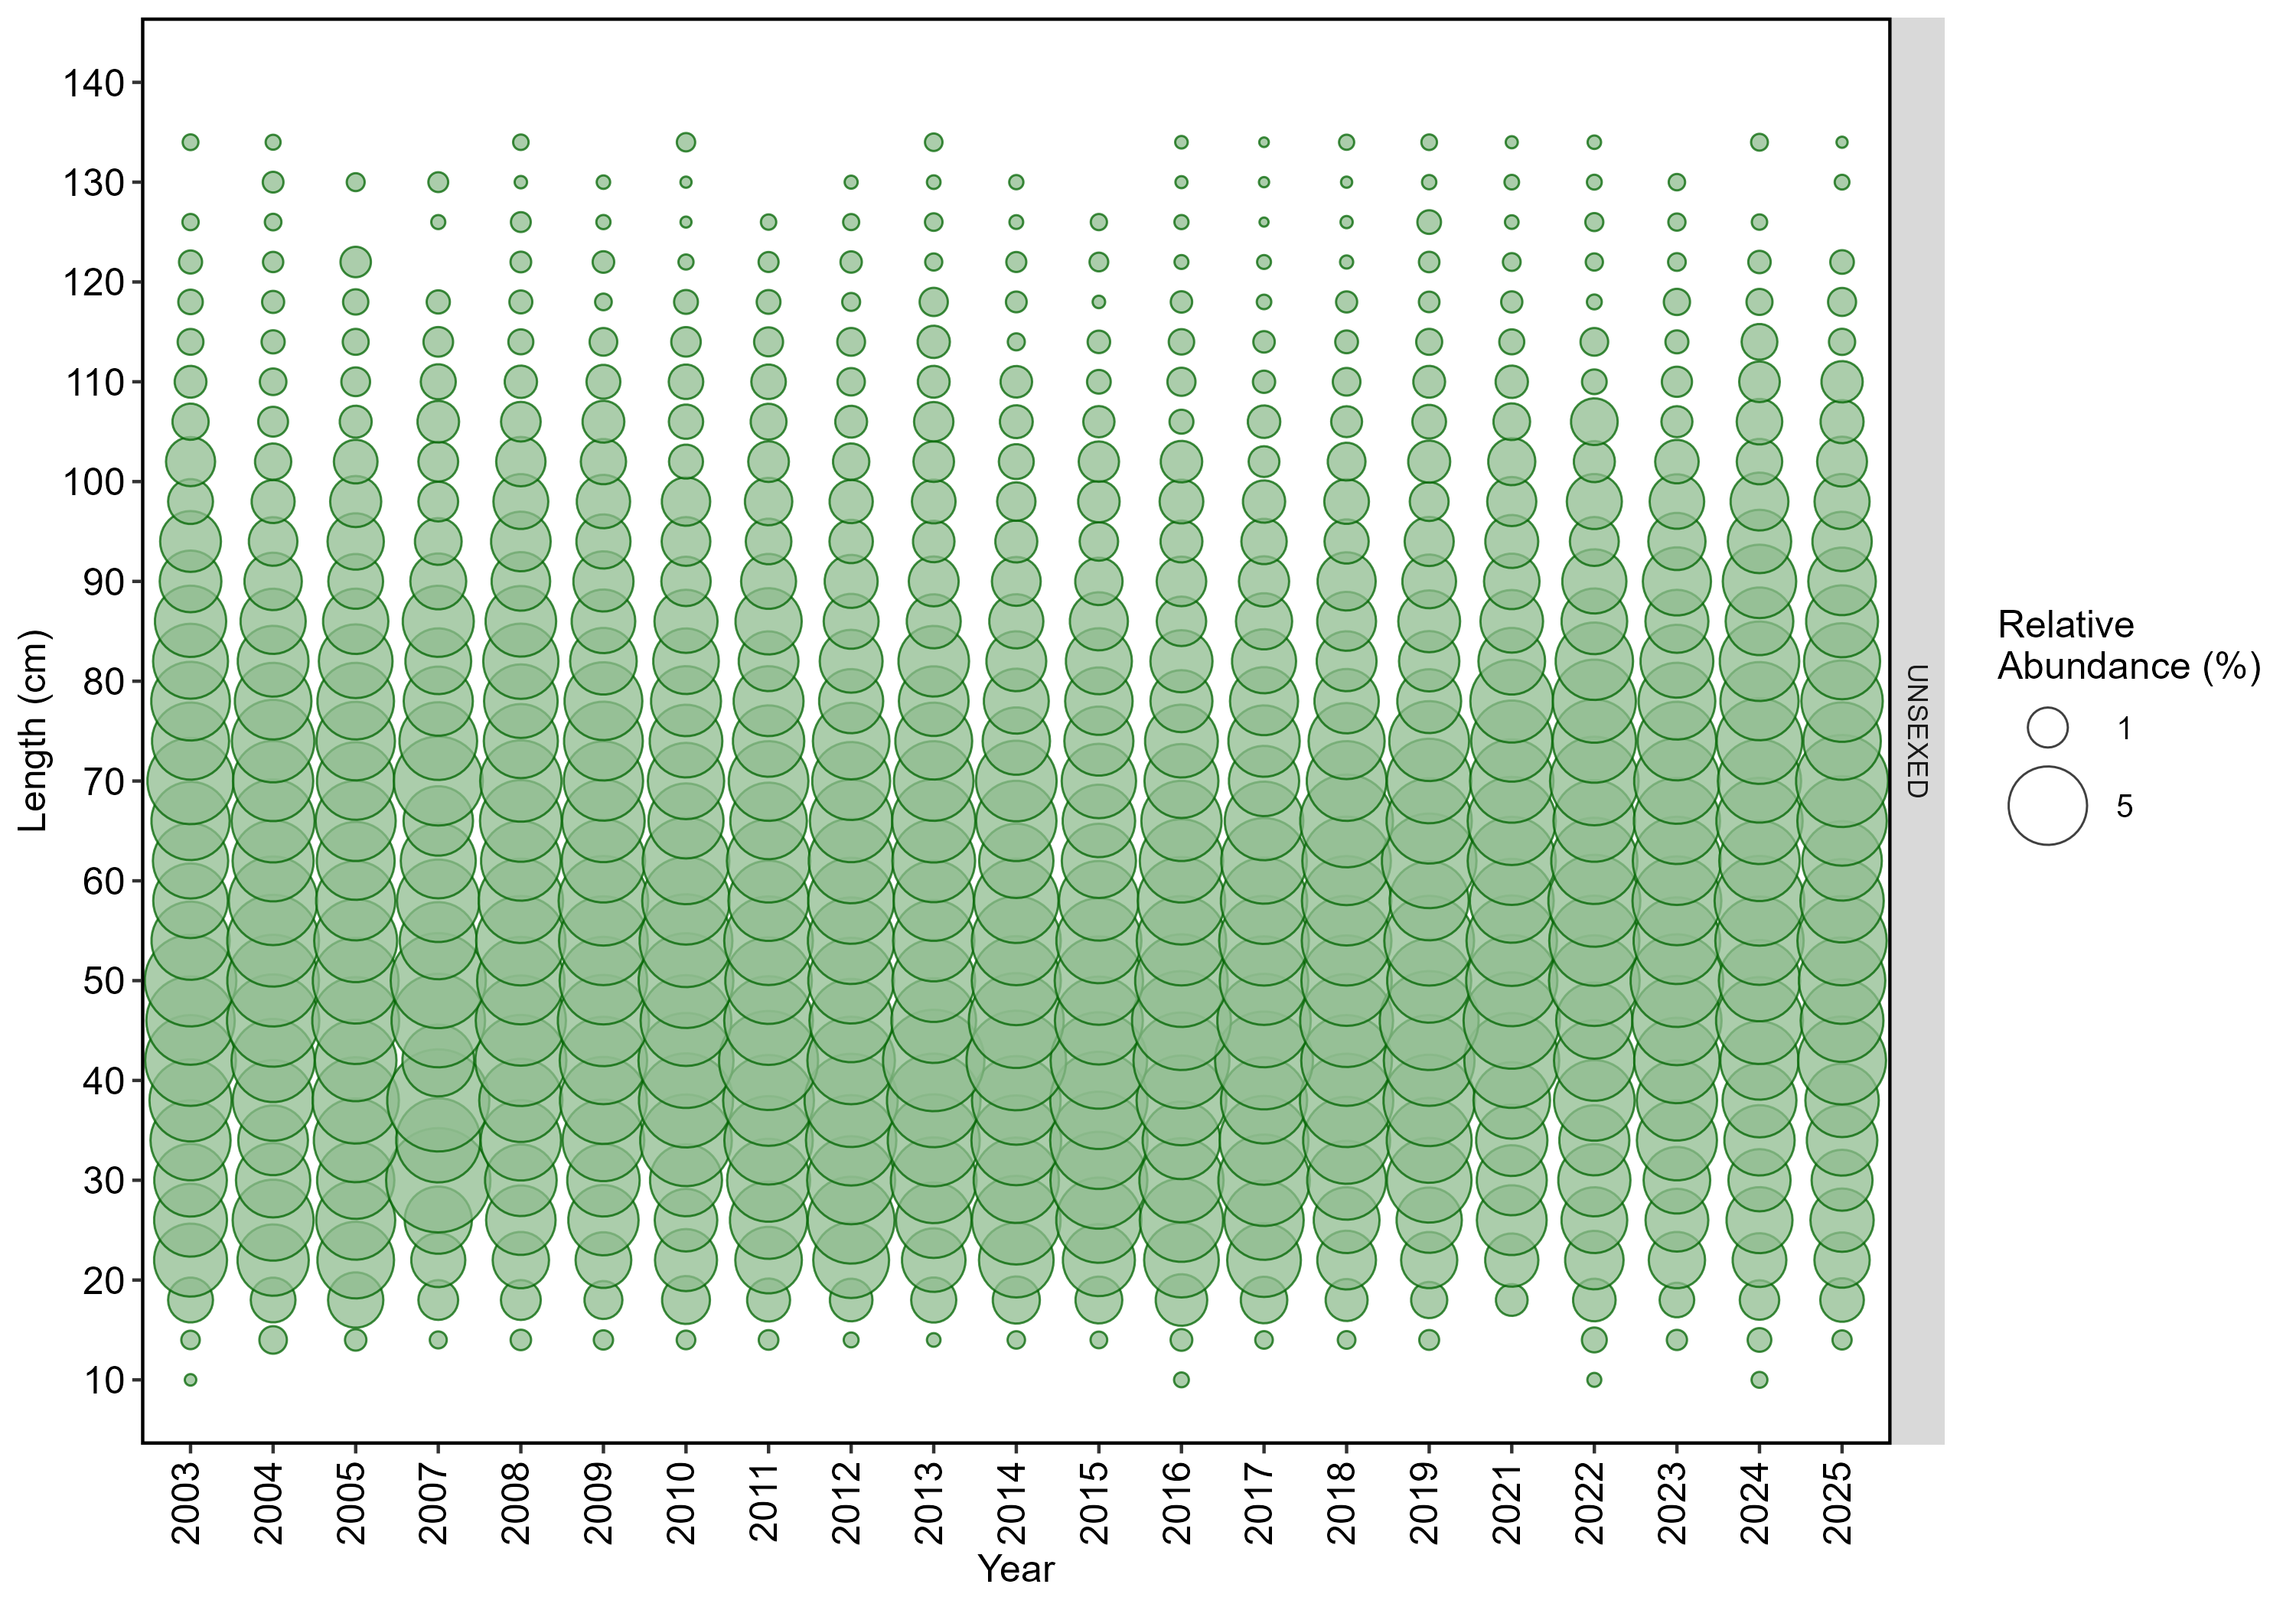
\includegraphics[width=0.95\linewidth,height=\textheight,keepaspectratio]{../plots/wcgbts_comps/plots/longnose skate_length_frequency_sex_0.png}

}

\caption{Length (cm) compostion data from the NWFSC WCGBTS for longnose
skate. Size of the circles within a year indicate higher (larger
circles) and lower (smaller circles) proportion observed by length bin.}

\end{figure}%

\newpage{}

\subsection{Longspine thornyhead}\label{longspine-thornyhead}

The most recent assessment of longspine thornyhead was a benchmark
assessment conducted in 2013. Across available data, longspine
thornyhead have been observed and sampled by the NWFSC WCGBTS. The NWFSC
WCGBTS observed longspine thornyhead on an average of 222 tows per year.
No validated (accurate and precise) aging methology currently exists for
longspine thornyhead. For this species, a total of 341 maturity samples
have been collected coastwide (regardless of stock area), with 63 read
maturities.

\begingroup\fontsize{10}{12}\selectfont
\begingroup\fontsize{10}{12}\selectfont

\begin{longtable}[t]{>{\raggedleft\arraybackslash}p{2cm}>{\raggedleft\arraybackslash}p{3.5cm}>{\raggedleft\arraybackslash}p{2cm}>{\raggedleft\arraybackslash}p{2cm}>{\raggedleft\arraybackslash}p{2cm}}
\caption{\label{tab:unnamed-chunk-346}Total number of available lengths, read ages, and unread age structures by data source and
state for longspine thornyhead.}\\
\toprule
State & Source & Lengths & Ages & Age Structures\\
\midrule
\endfirsthead
\caption[]{Total number of available lengths, read ages, and unread age structures by data source and
state for longspine thornyhead. (\textit{continued)}}\\
\toprule
State & Source & Lengths & Ages & Age Structures\\
\midrule
\endhead

\endfoot
\bottomrule
\endlastfoot
CA & NWFSC WCGBTS & 76,437 & 0 & 9,925\\
OR & NWFSC WCGBTS & 34,876 & 0 & 4,219\\
WA & NWFSC WCGBTS & 14,741 & 0 & 1,819\\*
\end{longtable}
\endgroup{}
\endgroup{}

\begin{figure}[H]

{\centering 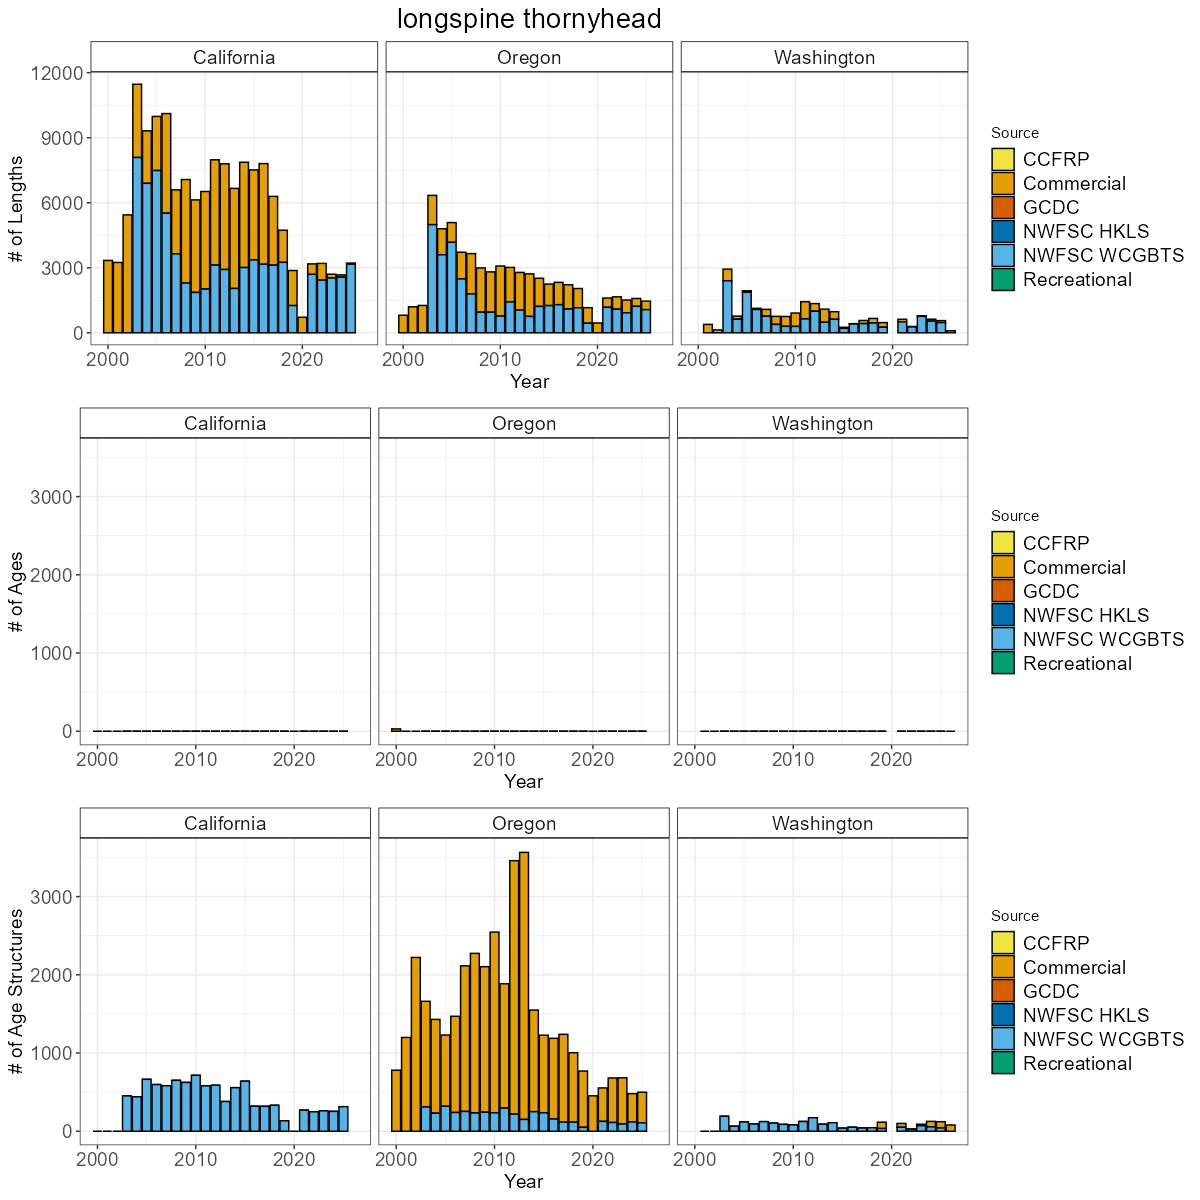
\includegraphics[width=0.95\linewidth,height=\textheight,keepaspectratio]{../plots/state_comparisons/longspine_thornyhead_state_compositions.png}

}

\caption{Total number of available lengths, read ages, and unread age
structures by data source by year for longspine thornyhead. Note the
y-axis maximum may differ by data type.}

\end{figure}%

\begin{figure}[H]

{\centering 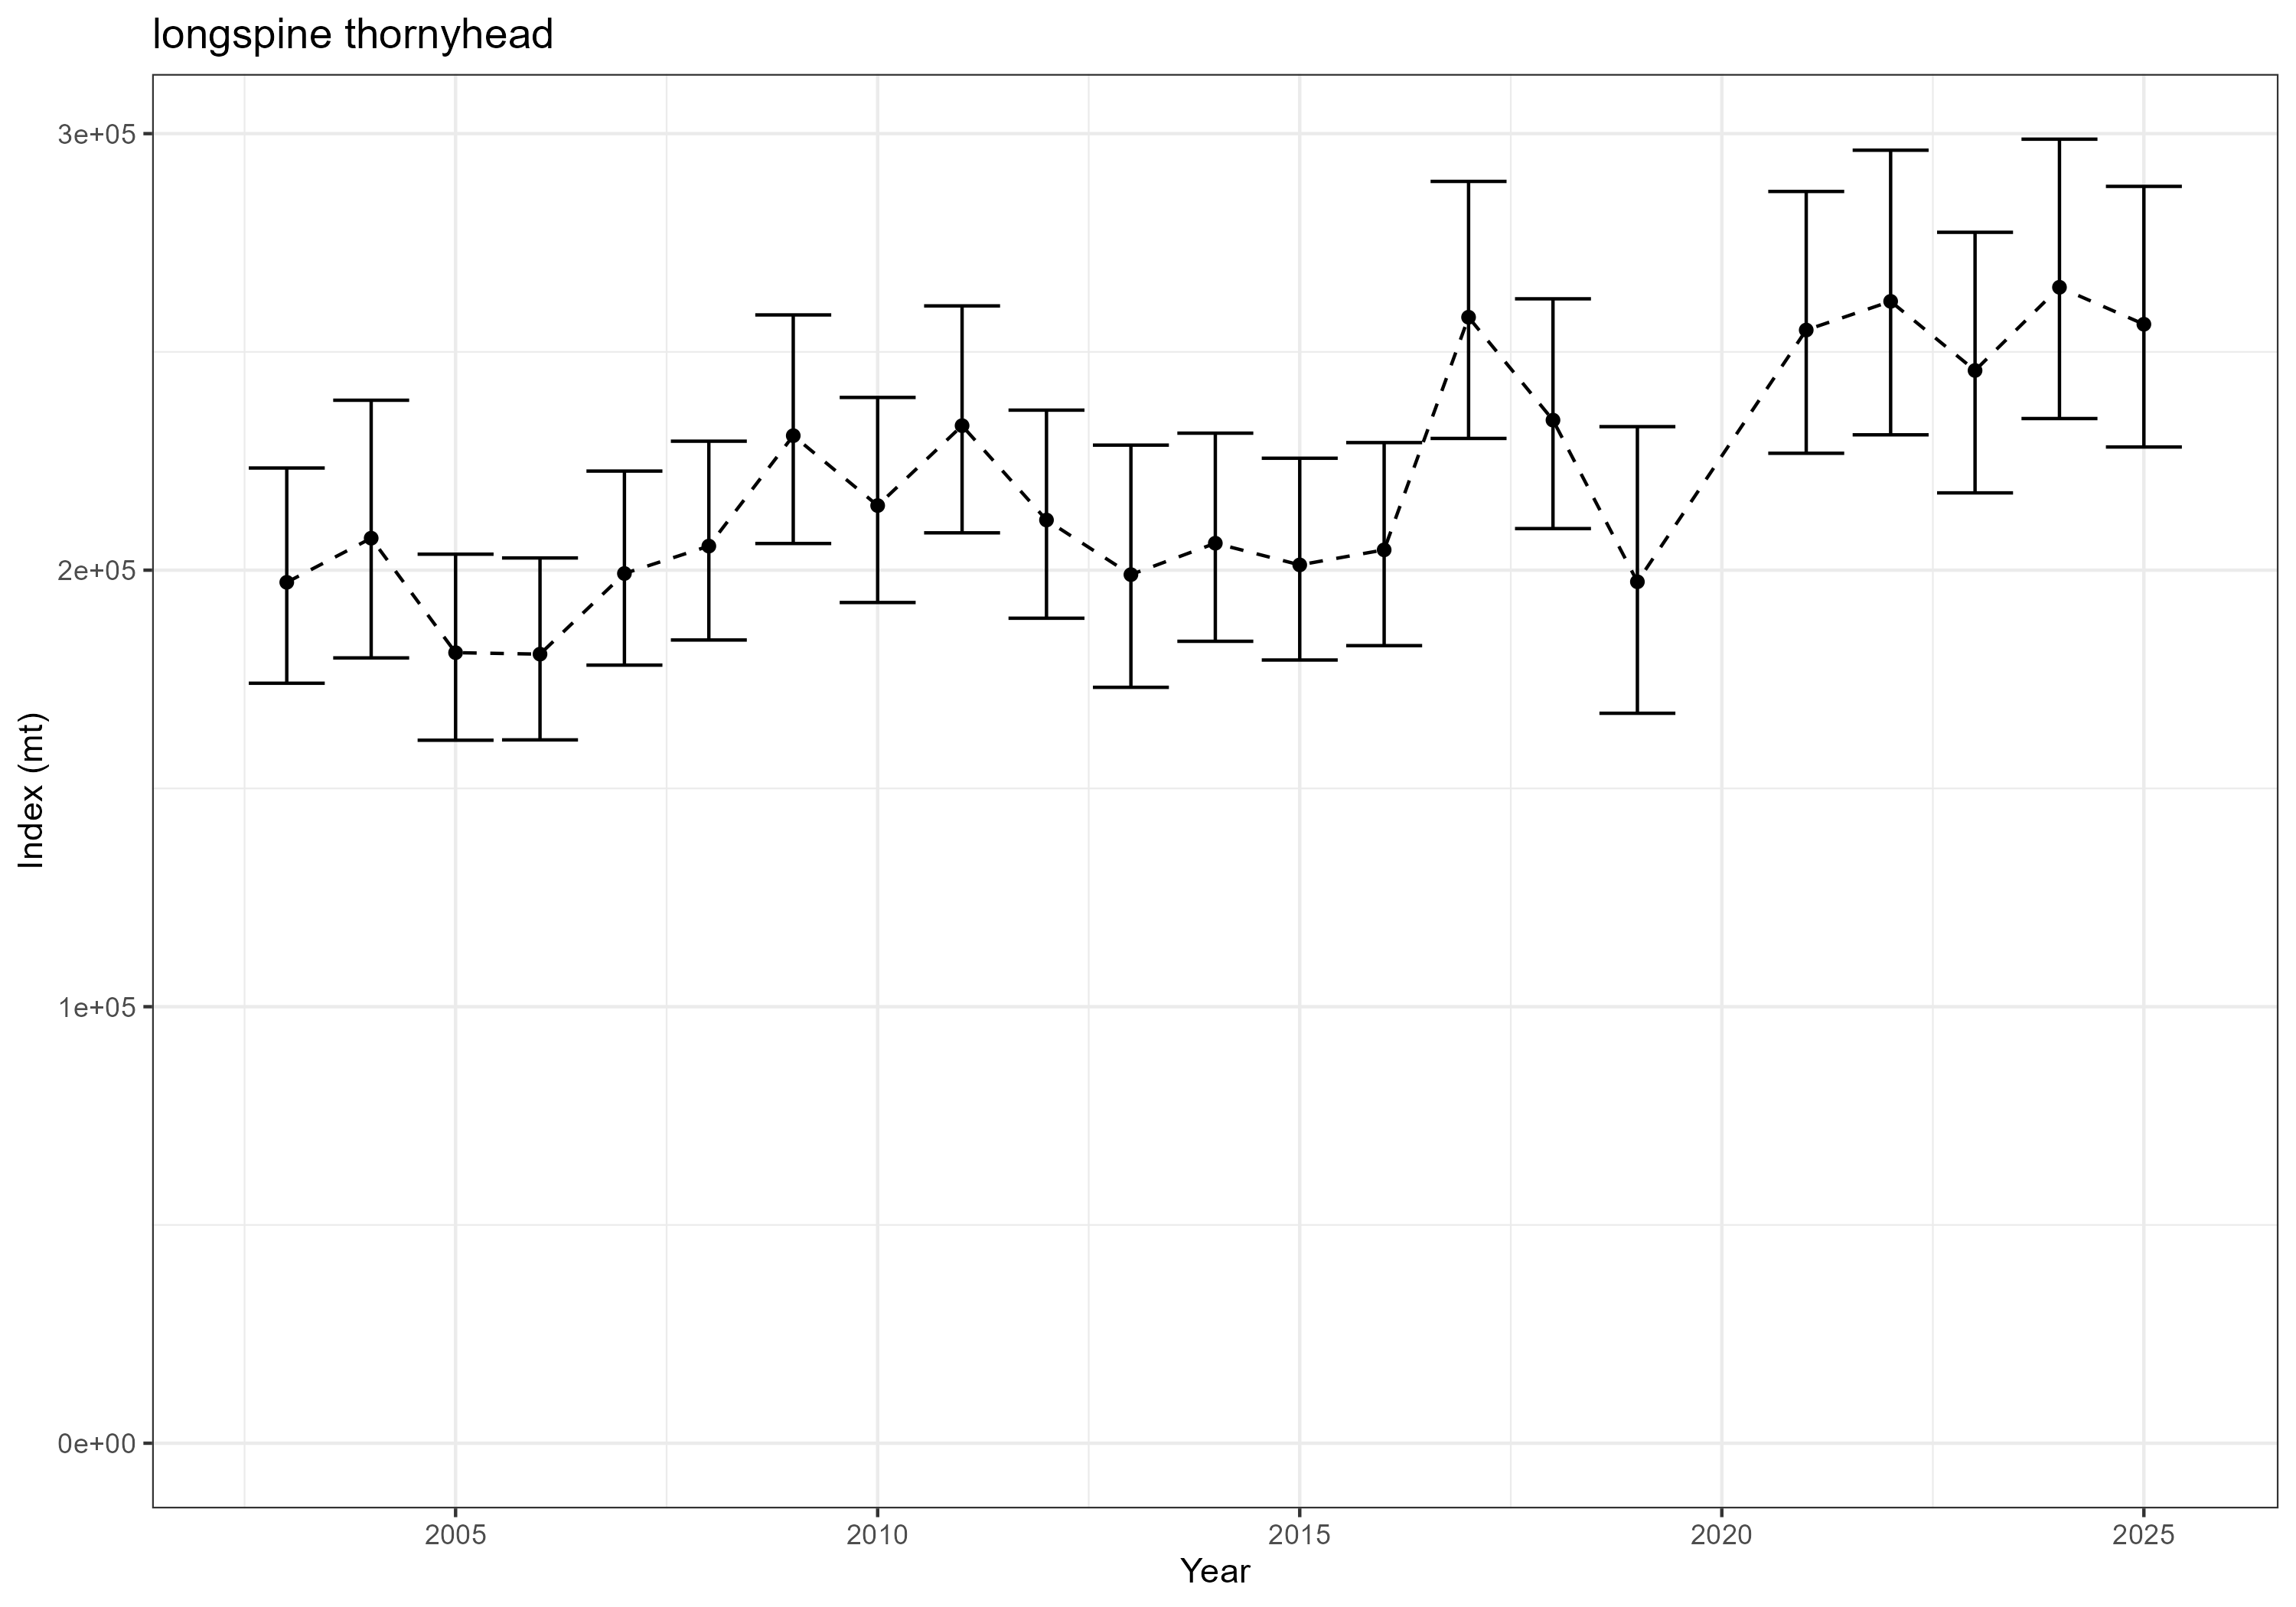
\includegraphics[width=0.95\linewidth,height=\textheight,keepaspectratio]{../plots/wcgbts_indices/longspine_thornyhead_index.png}

}

\caption{Estimated relative index of abundance for longspine thornyhead
from the NWFSC WCGBTS.}

\end{figure}%

\begin{figure}[H]

{\centering 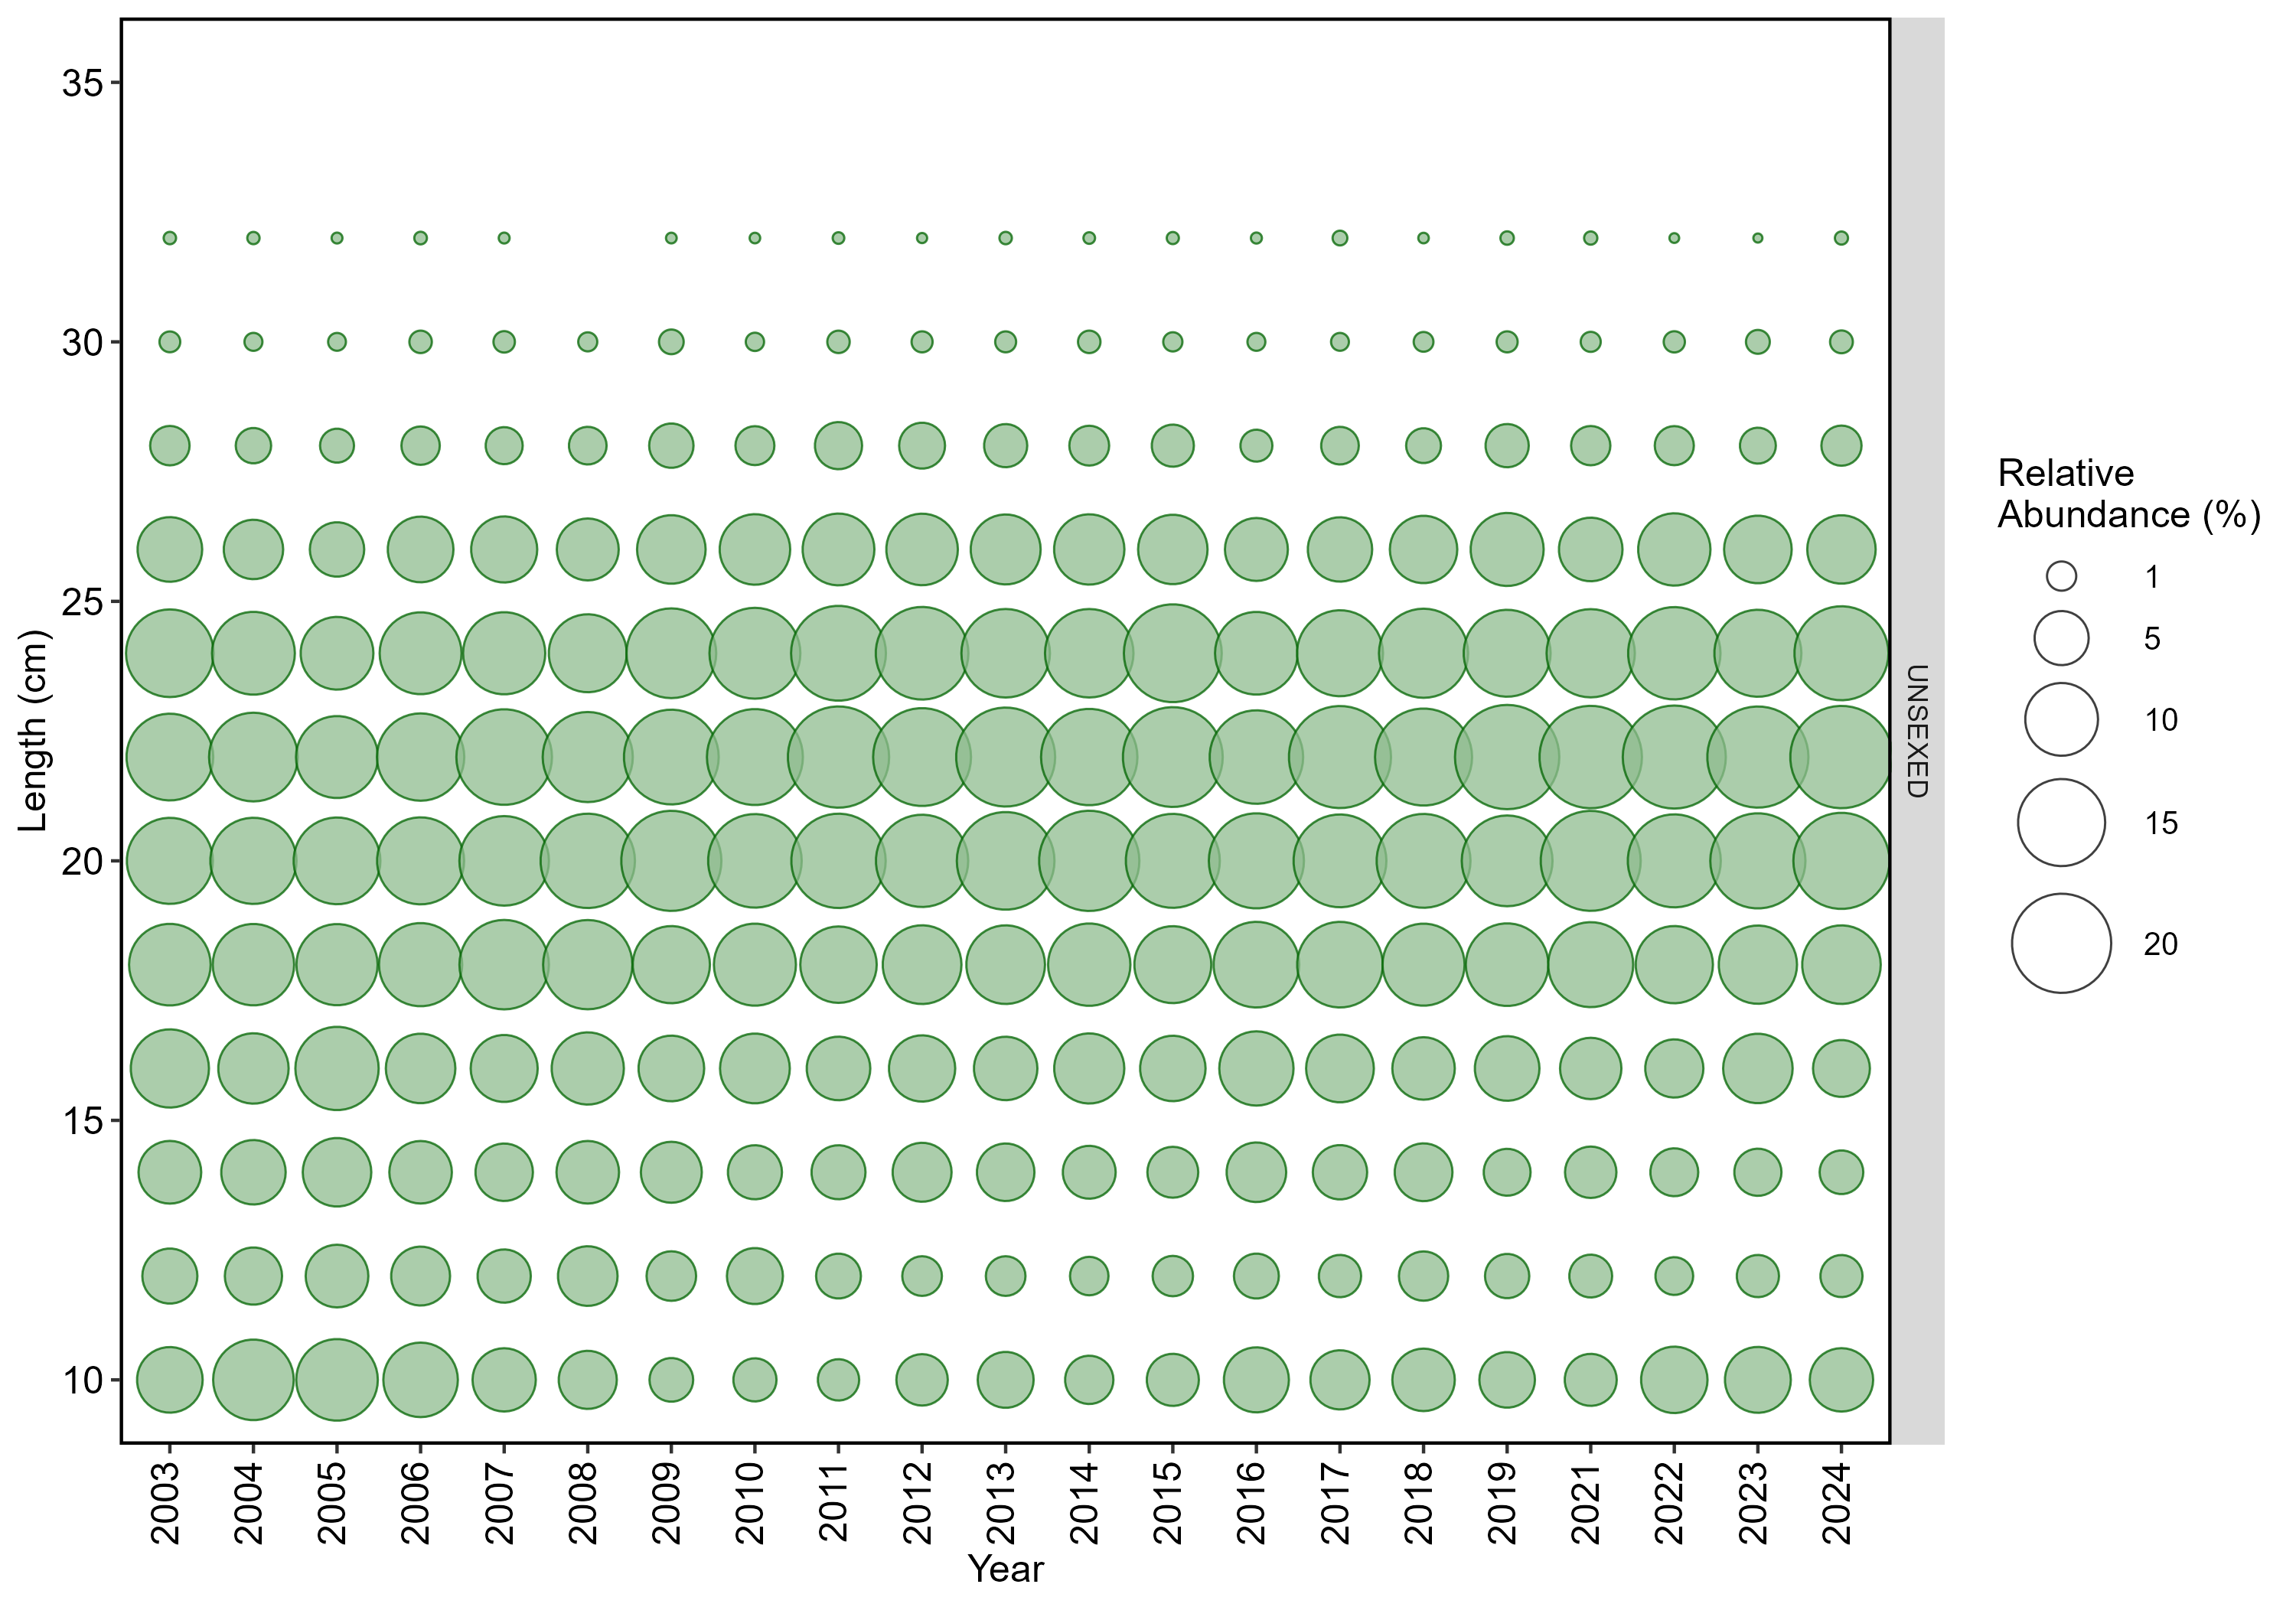
\includegraphics[width=0.95\linewidth,height=\textheight,keepaspectratio]{../plots/wcgbts_comps/plots/longspine thornyhead_length_frequency_sex_0.png}

}

\caption{Length (cm) compostion data from the NWFSC WCGBTS for longspine
thornyhead. Size of the circles within a year indicate higher (larger
circles) and lower (smaller circles) proportion observed by length bin.}

\end{figure}%

\newpage{}

\subsection{Pacific cod}\label{pacific-cod}

To date, no assessment or analysis has been conducted on Pacific cod.
Across available data, Pacific cod have been observed and sampled by the
NWFSC WCGBTS. The NWFSC WCGBTS observed Pacific cod on an average of 28
tows per year. For this species, a total of 125 maturity samples have
been collected coastwide (regardless of stock area), with 0 read
maturities.

\begingroup\fontsize{10}{12}\selectfont
\begingroup\fontsize{10}{12}\selectfont

\begin{longtable}[t]{>{\raggedleft\arraybackslash}p{2cm}>{\raggedleft\arraybackslash}p{3.5cm}>{\raggedleft\arraybackslash}p{2cm}>{\raggedleft\arraybackslash}p{2cm}>{\raggedleft\arraybackslash}p{2cm}}
\caption{\label{tab:unnamed-chunk-363}Total number of available lengths, read ages, and unread age structures by data source and
state for Pacific cod.}\\
\toprule
State & Source & Lengths & Ages & Age Structures\\
\midrule
\endfirsthead
\caption[]{Total number of available lengths, read ages, and unread age structures by data source and
state for Pacific cod. (\textit{continued)}}\\
\toprule
State & Source & Lengths & Ages & Age Structures\\
\midrule
\endhead

\endfoot
\bottomrule
\endlastfoot
CA & NWFSC WCGBTS & 14 & 0 & 0\\
OR & NWFSC WCGBTS & 515 & 0 & 219\\
WA & NWFSC WCGBTS & 3,852 & 0 & 1,413\\*
\end{longtable}
\endgroup{}
\endgroup{}

\begin{figure}[H]

{\centering 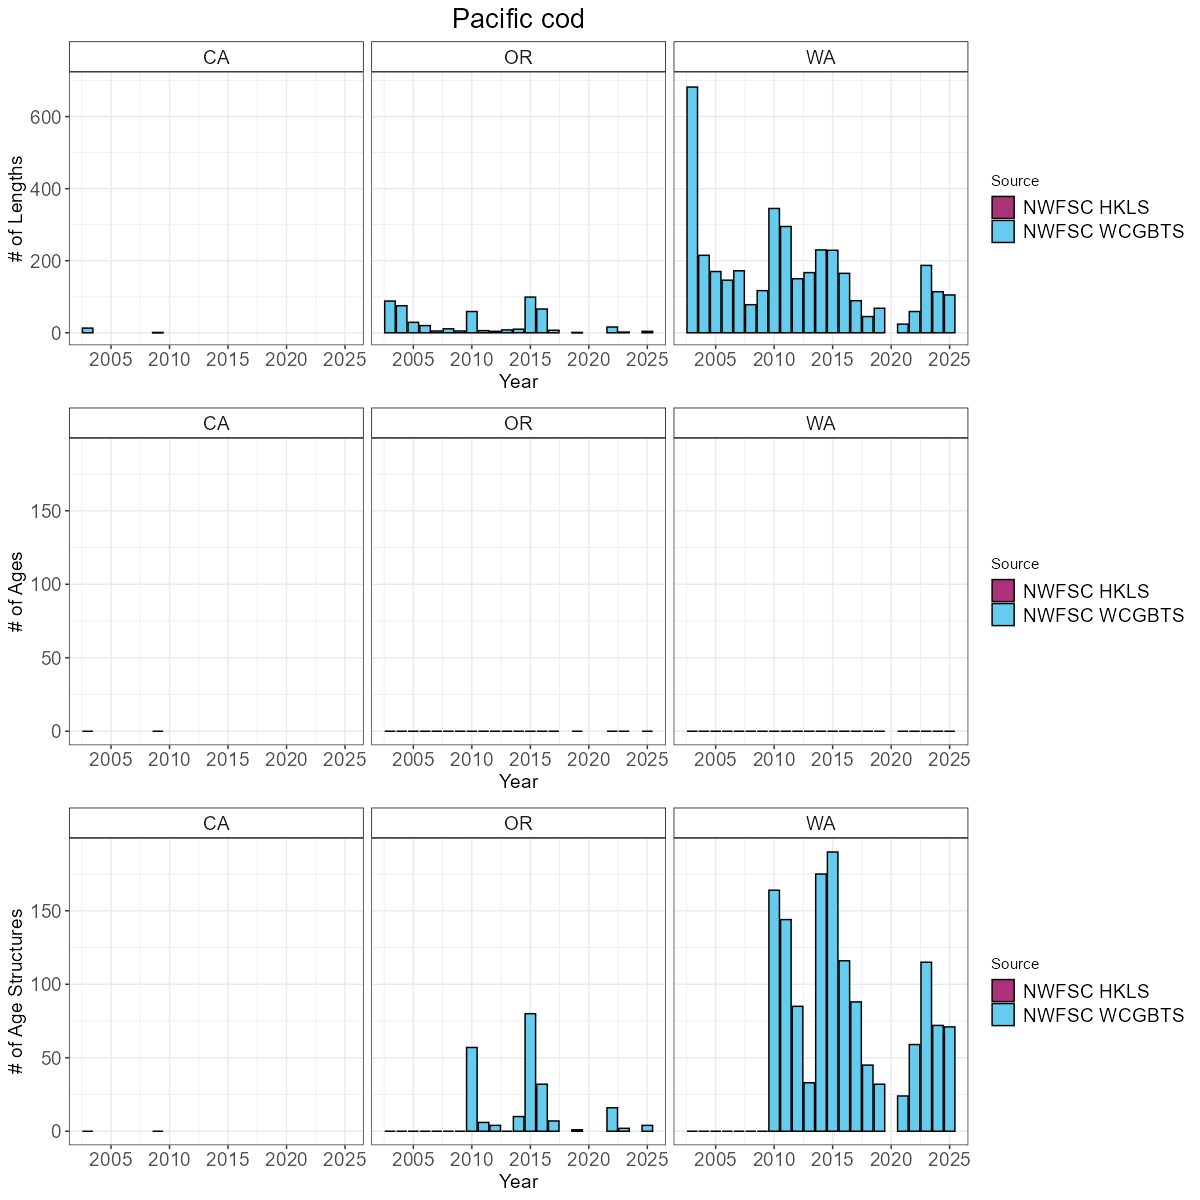
\includegraphics[width=0.95\linewidth,height=\textheight,keepaspectratio]{../plots/state_comparisons/pacific_cod_state_compositions.png}

}

\caption{Total number of available lengths, read ages, and unread age
structures by data source by year for Pacific cod. Note the y-axis
maximum may differ by data type.}

\end{figure}%

\begin{figure}[H]

{\centering 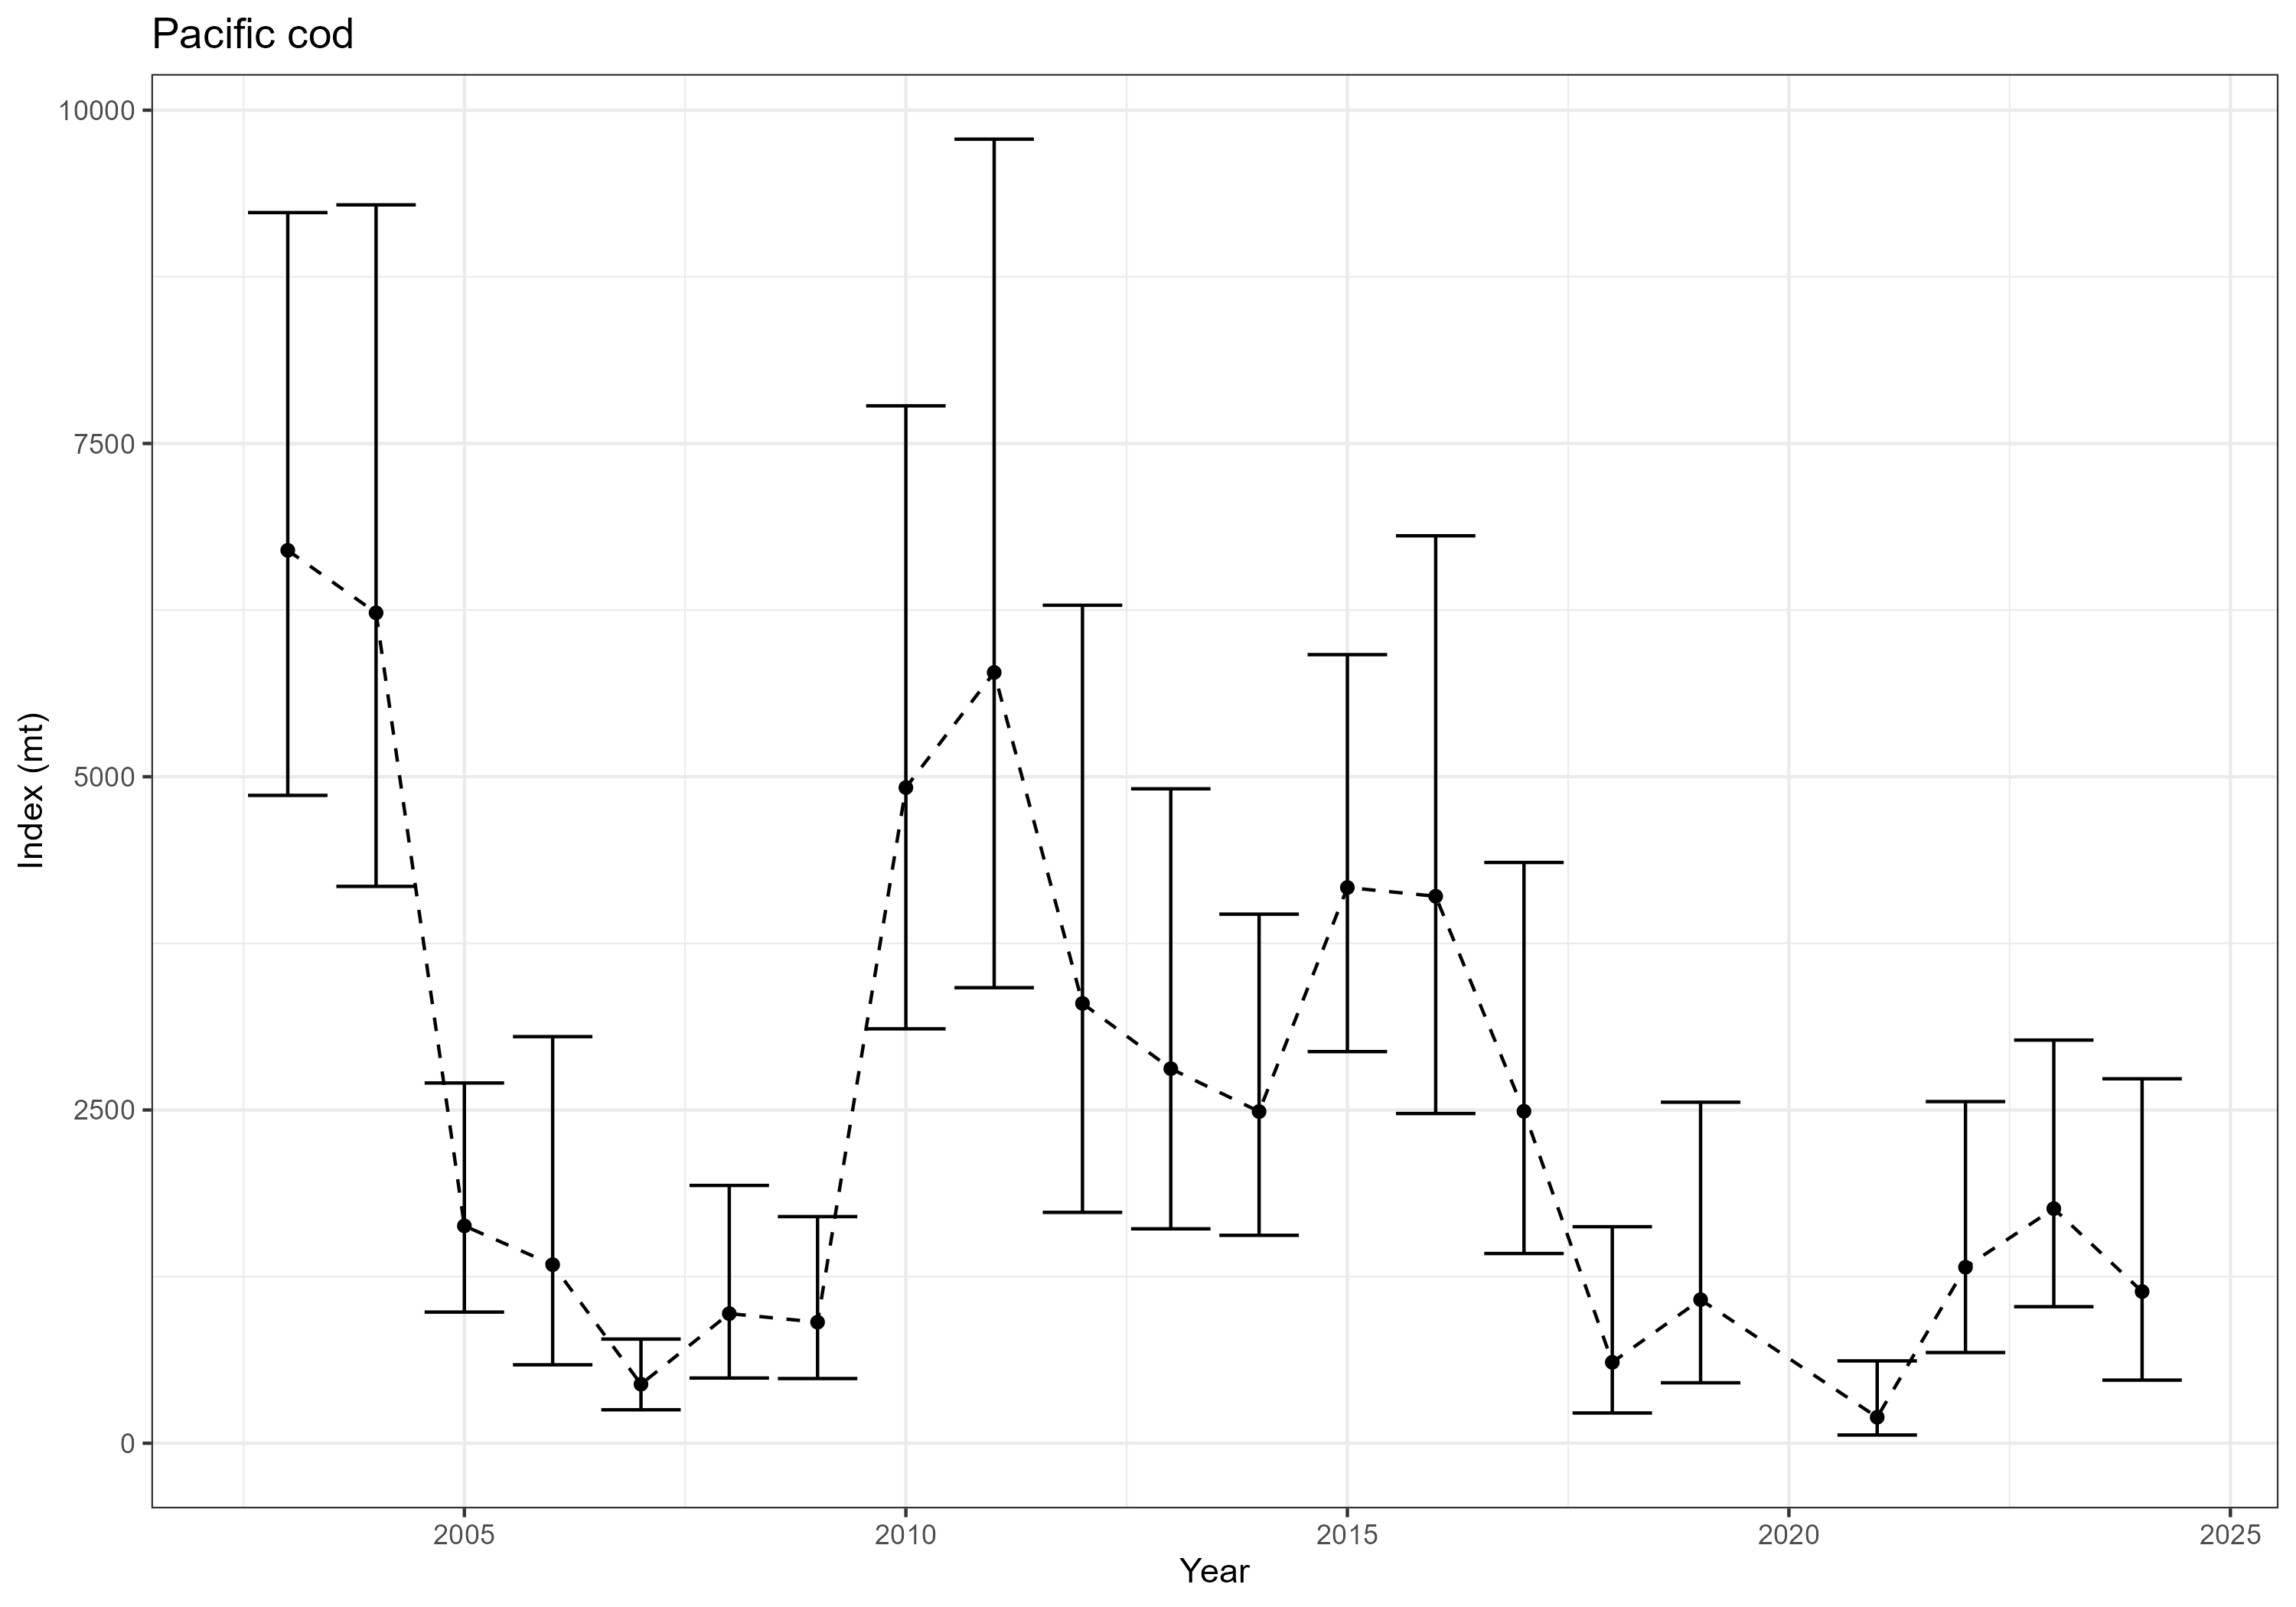
\includegraphics[width=0.95\linewidth,height=\textheight,keepaspectratio]{../plots/wcgbts_indices/pacific_cod_index.png}

}

\caption{Estimated relative index of abundance for Pacific cod from the
NWFSC WCGBTS.}

\end{figure}%

\begin{figure}[H]

{\centering 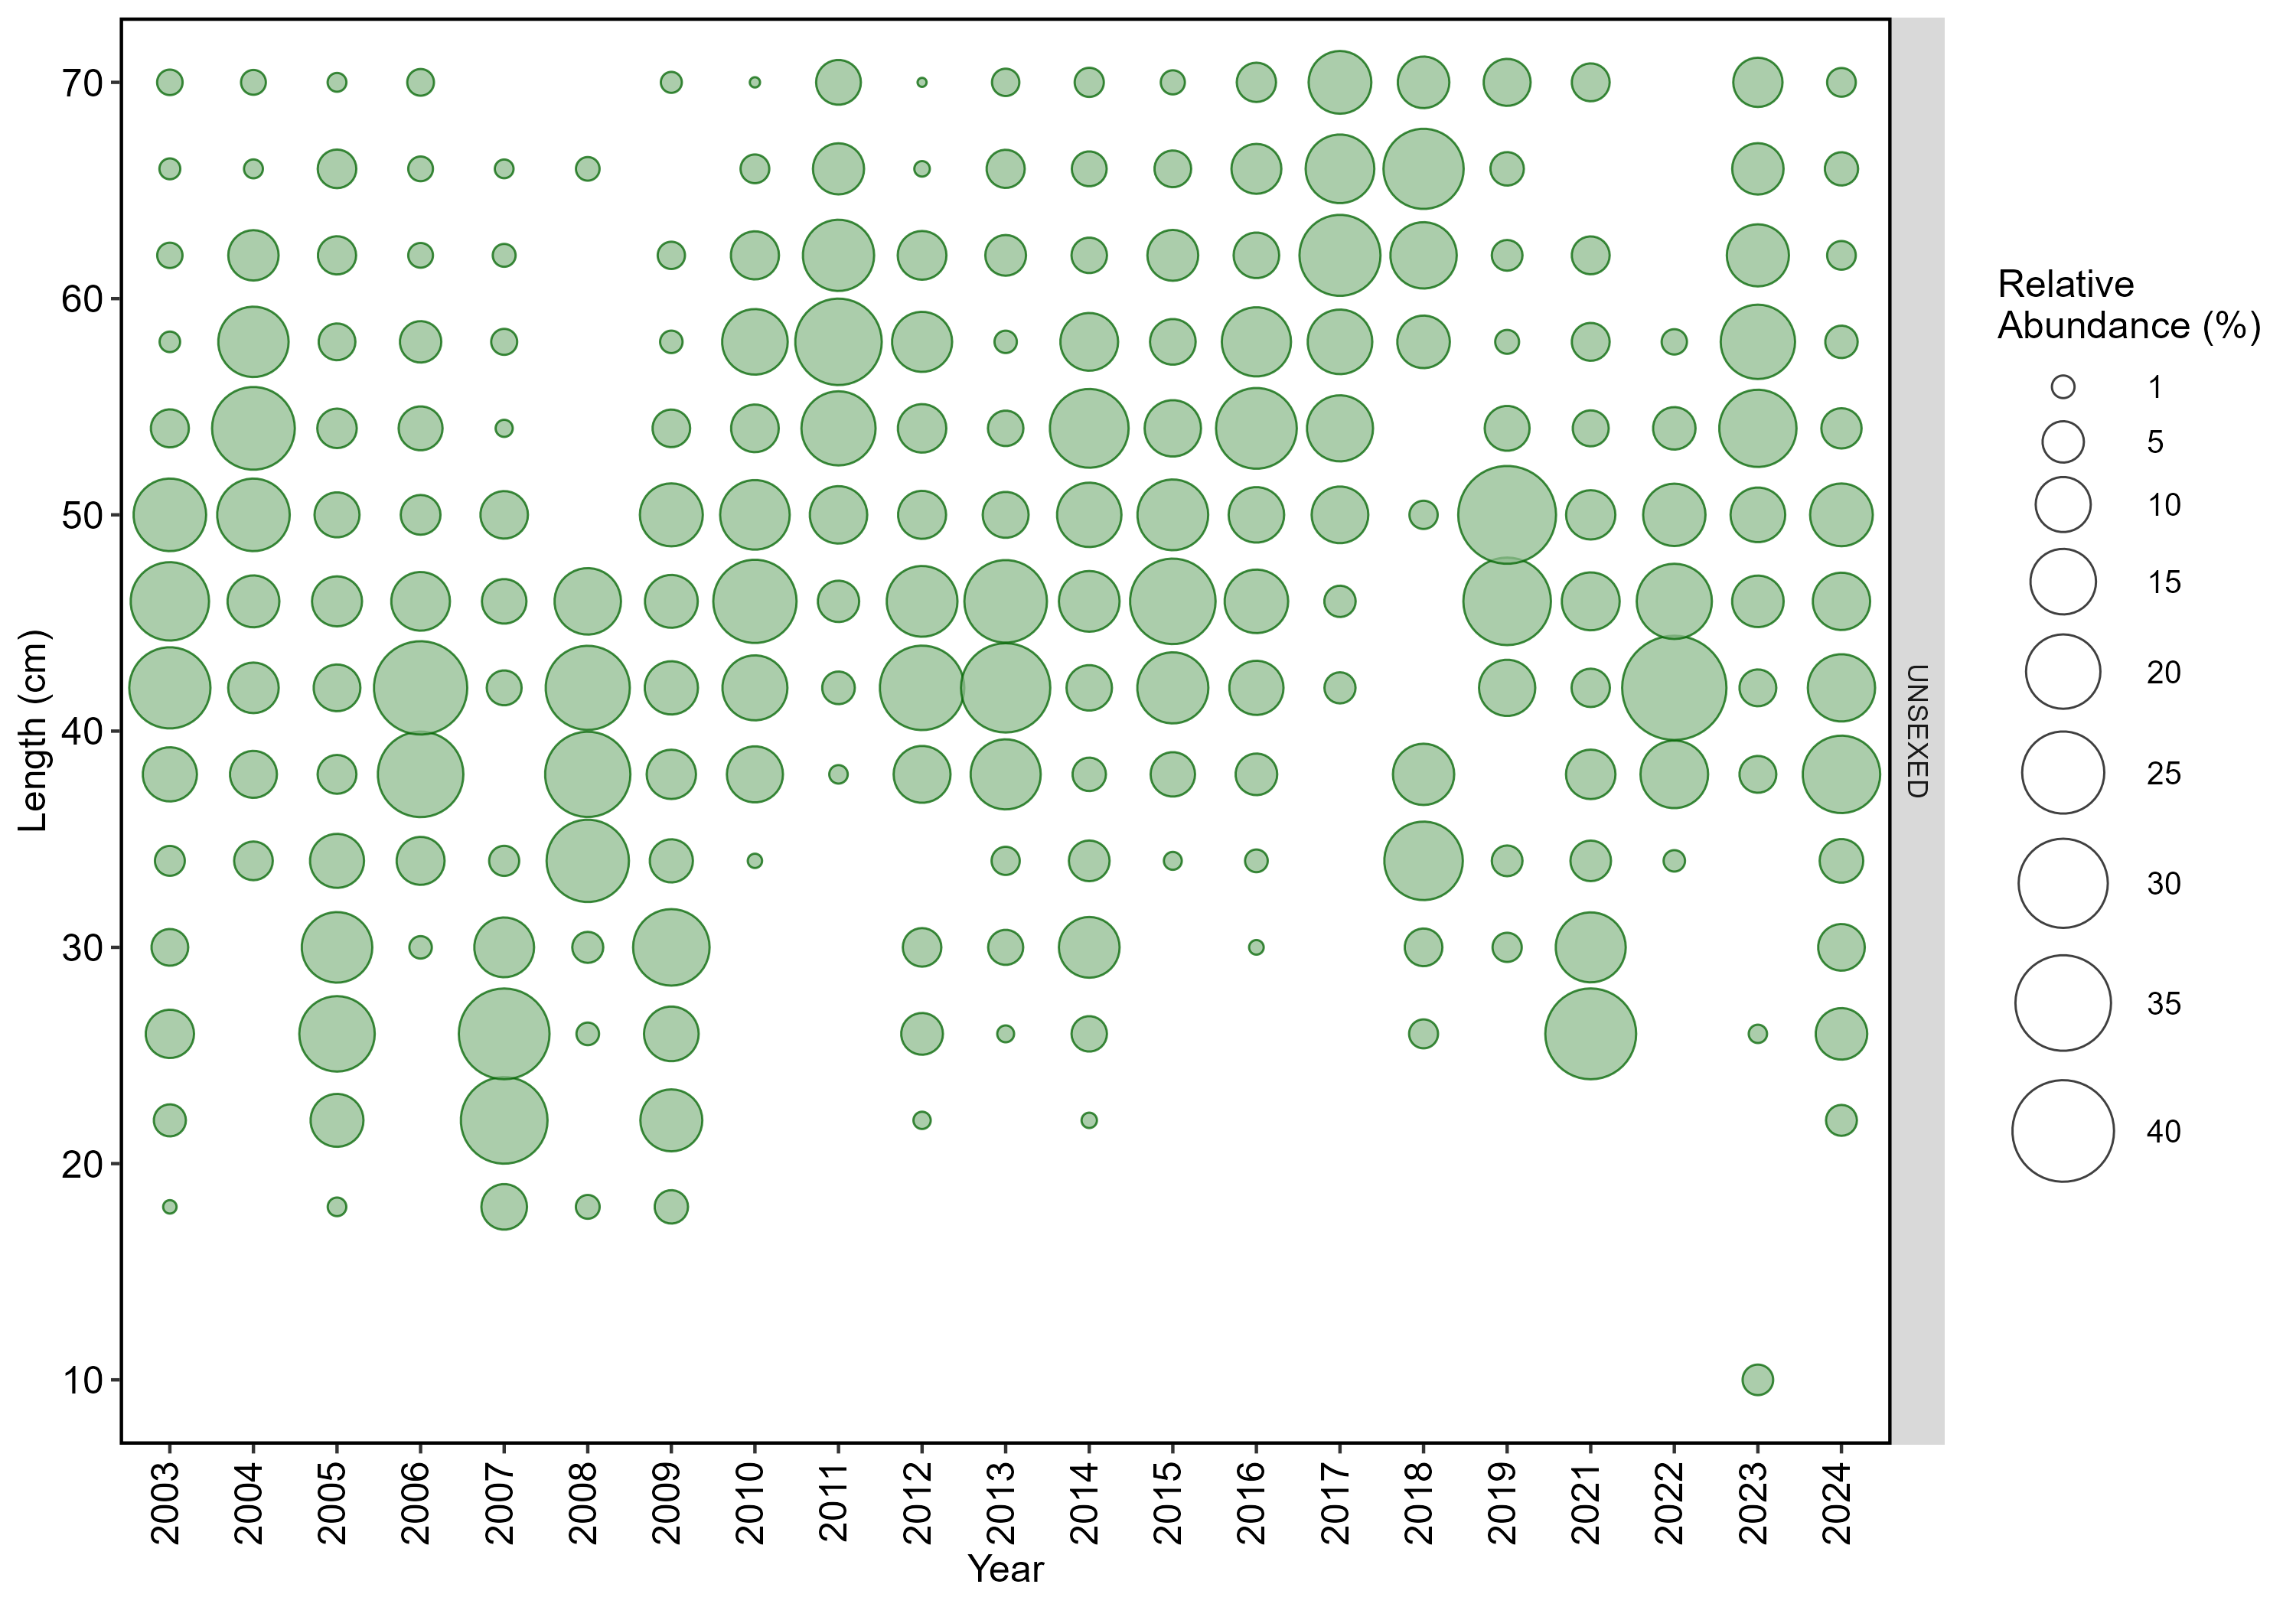
\includegraphics[width=0.95\linewidth,height=\textheight,keepaspectratio]{../plots/wcgbts_comps/plots/Pacific cod_length_frequency_sex_0.png}

}

\caption{Length (cm) compostion data from the NWFSC WCGBTS for Pacific
cod. Size of the circles within a year indicate higher (larger circles)
and lower (smaller circles) proportion observed by length bin.}

\end{figure}%

\newpage{}

\subsection{Pacific ocean perch}\label{pacific-ocean-perch}

The most recent assessment of Pacific ocean perch was a benchmark
assessment conducted in 2017. Across available data, Pacific ocean perch
have been observed and sampled by the NWFSC WCGBTS. The NWFSC WCGBTS
observed Pacific ocean perch on an average of 48 tows per year. For this
species, a total of 583 maturity samples have been collected coastwide
(regardless of stock area), with 583 read maturities.

\begingroup\fontsize{10}{12}\selectfont
\begingroup\fontsize{10}{12}\selectfont

\begin{longtable}[t]{>{\raggedleft\arraybackslash}p{2cm}>{\raggedleft\arraybackslash}p{3.5cm}>{\raggedleft\arraybackslash}p{2cm}>{\raggedleft\arraybackslash}p{2cm}>{\raggedleft\arraybackslash}p{2cm}}
\caption{\label{tab:unnamed-chunk-380}Total number of available lengths, read ages, and unread age structures by data source and
state for Pacific ocean perch.}\\
\toprule
State & Source & Lengths & Ages & Age Structures\\
\midrule
\endfirsthead
\caption[]{Total number of available lengths, read ages, and unread age structures by data source and
state for Pacific ocean perch. (\textit{continued)}}\\
\toprule
State & Source & Lengths & Ages & Age Structures\\
\midrule
\endhead

\endfoot
\bottomrule
\endlastfoot
CA & NWFSC WCGBTS & 254 & 78 & 175\\
OR & NWFSC WCGBTS & 10,249 & 3,061 & 4,198\\
WA & NWFSC WCGBTS & 8,268 & 2,743 & 2,089\\*
\end{longtable}
\endgroup{}
\endgroup{}

\begin{figure}[H]

{\centering 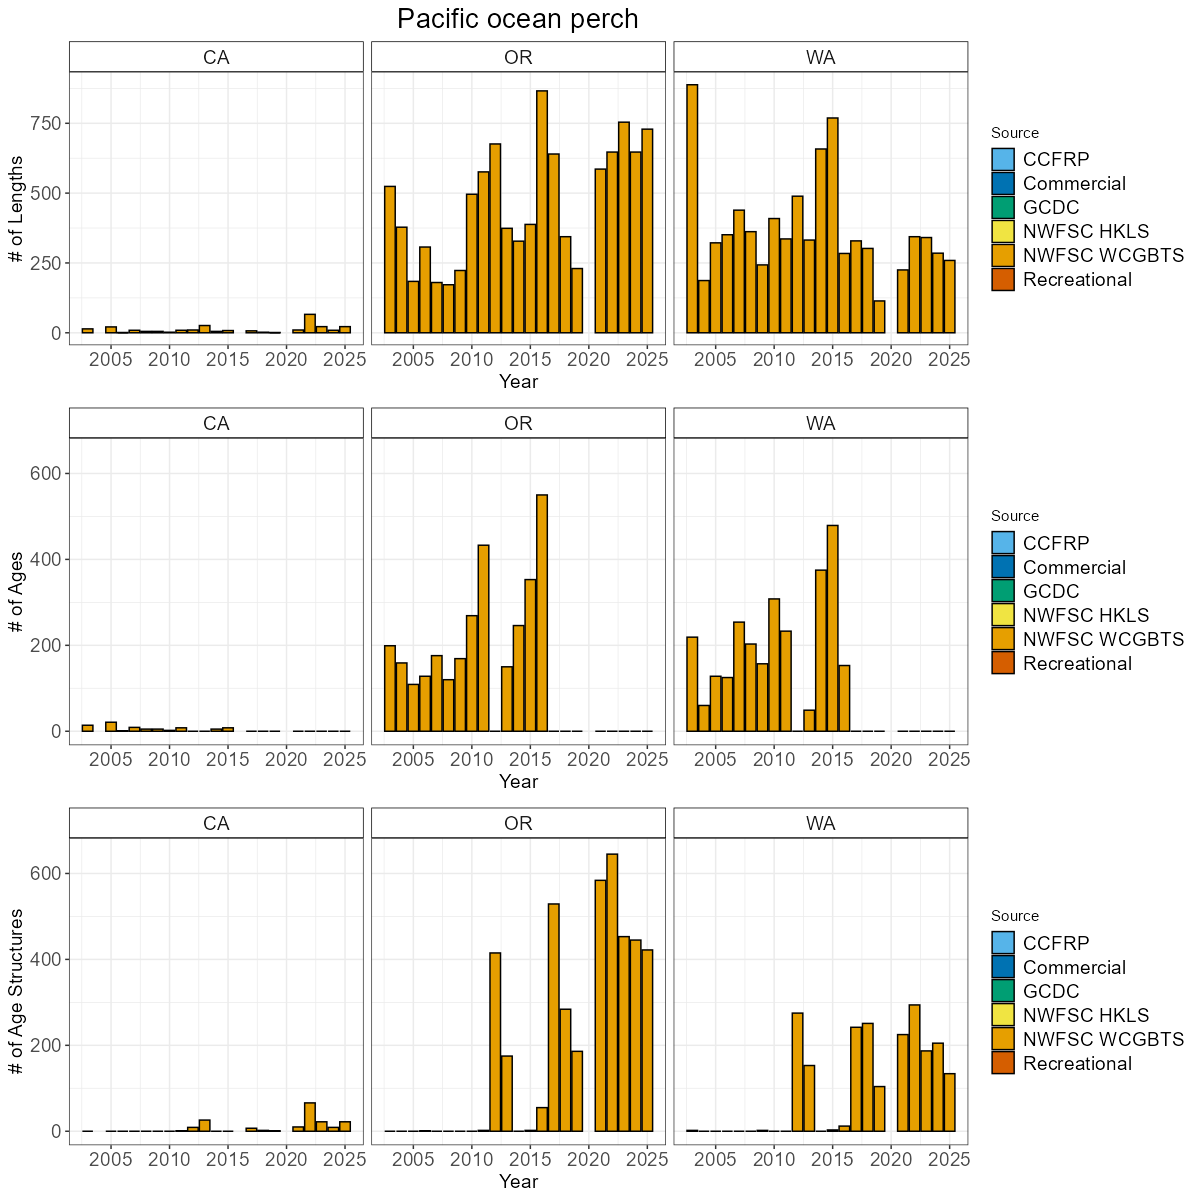
\includegraphics[width=0.95\linewidth,height=\textheight,keepaspectratio]{../plots/state_comparisons/pacific_ocean_perch_state_compositions.png}

}

\caption{Total number of available lengths, read ages, and unread age
structures by data source by year for Pacific ocean perch. Note the
y-axis maximum may differ by data type.}

\end{figure}%

\begin{figure}[H]

{\centering 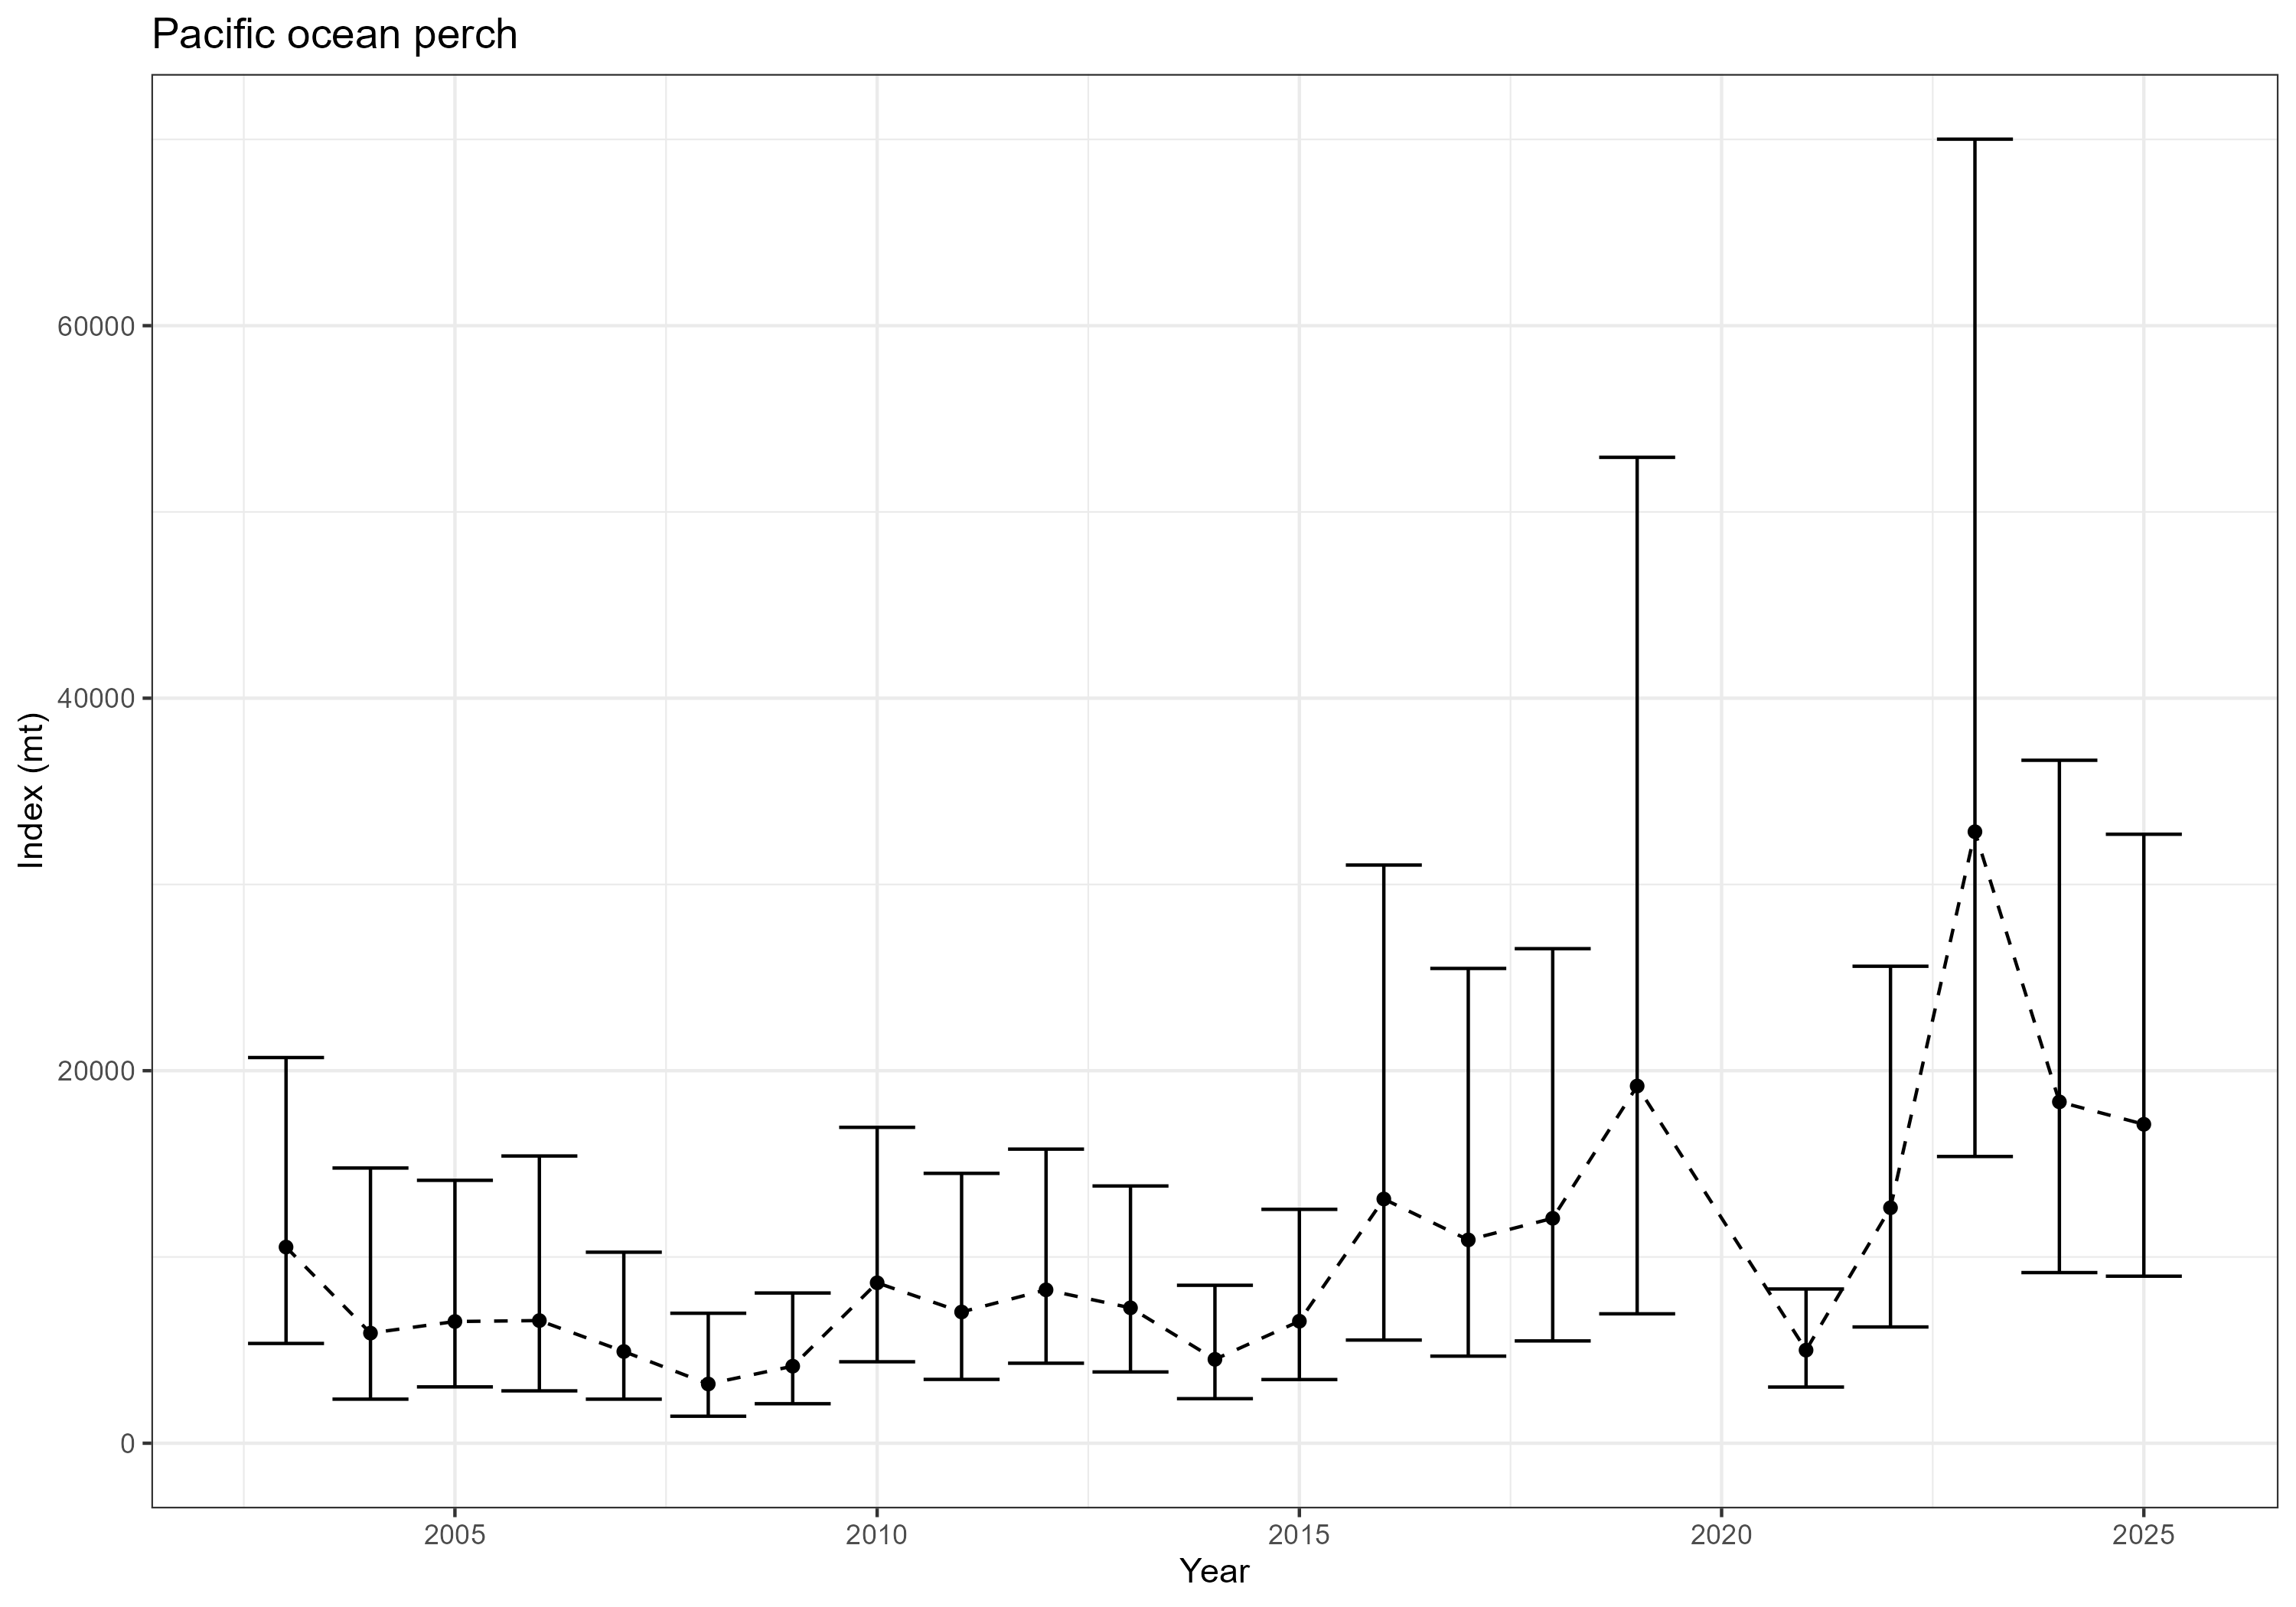
\includegraphics[width=0.95\linewidth,height=\textheight,keepaspectratio]{../plots/wcgbts_indices/pacific_ocean_perch_index.png}

}

\caption{Estimated relative index of abundance for Pacific ocean perch
from the NWFSC WCGBTS.}

\end{figure}%

\begin{figure}[H]

{\centering 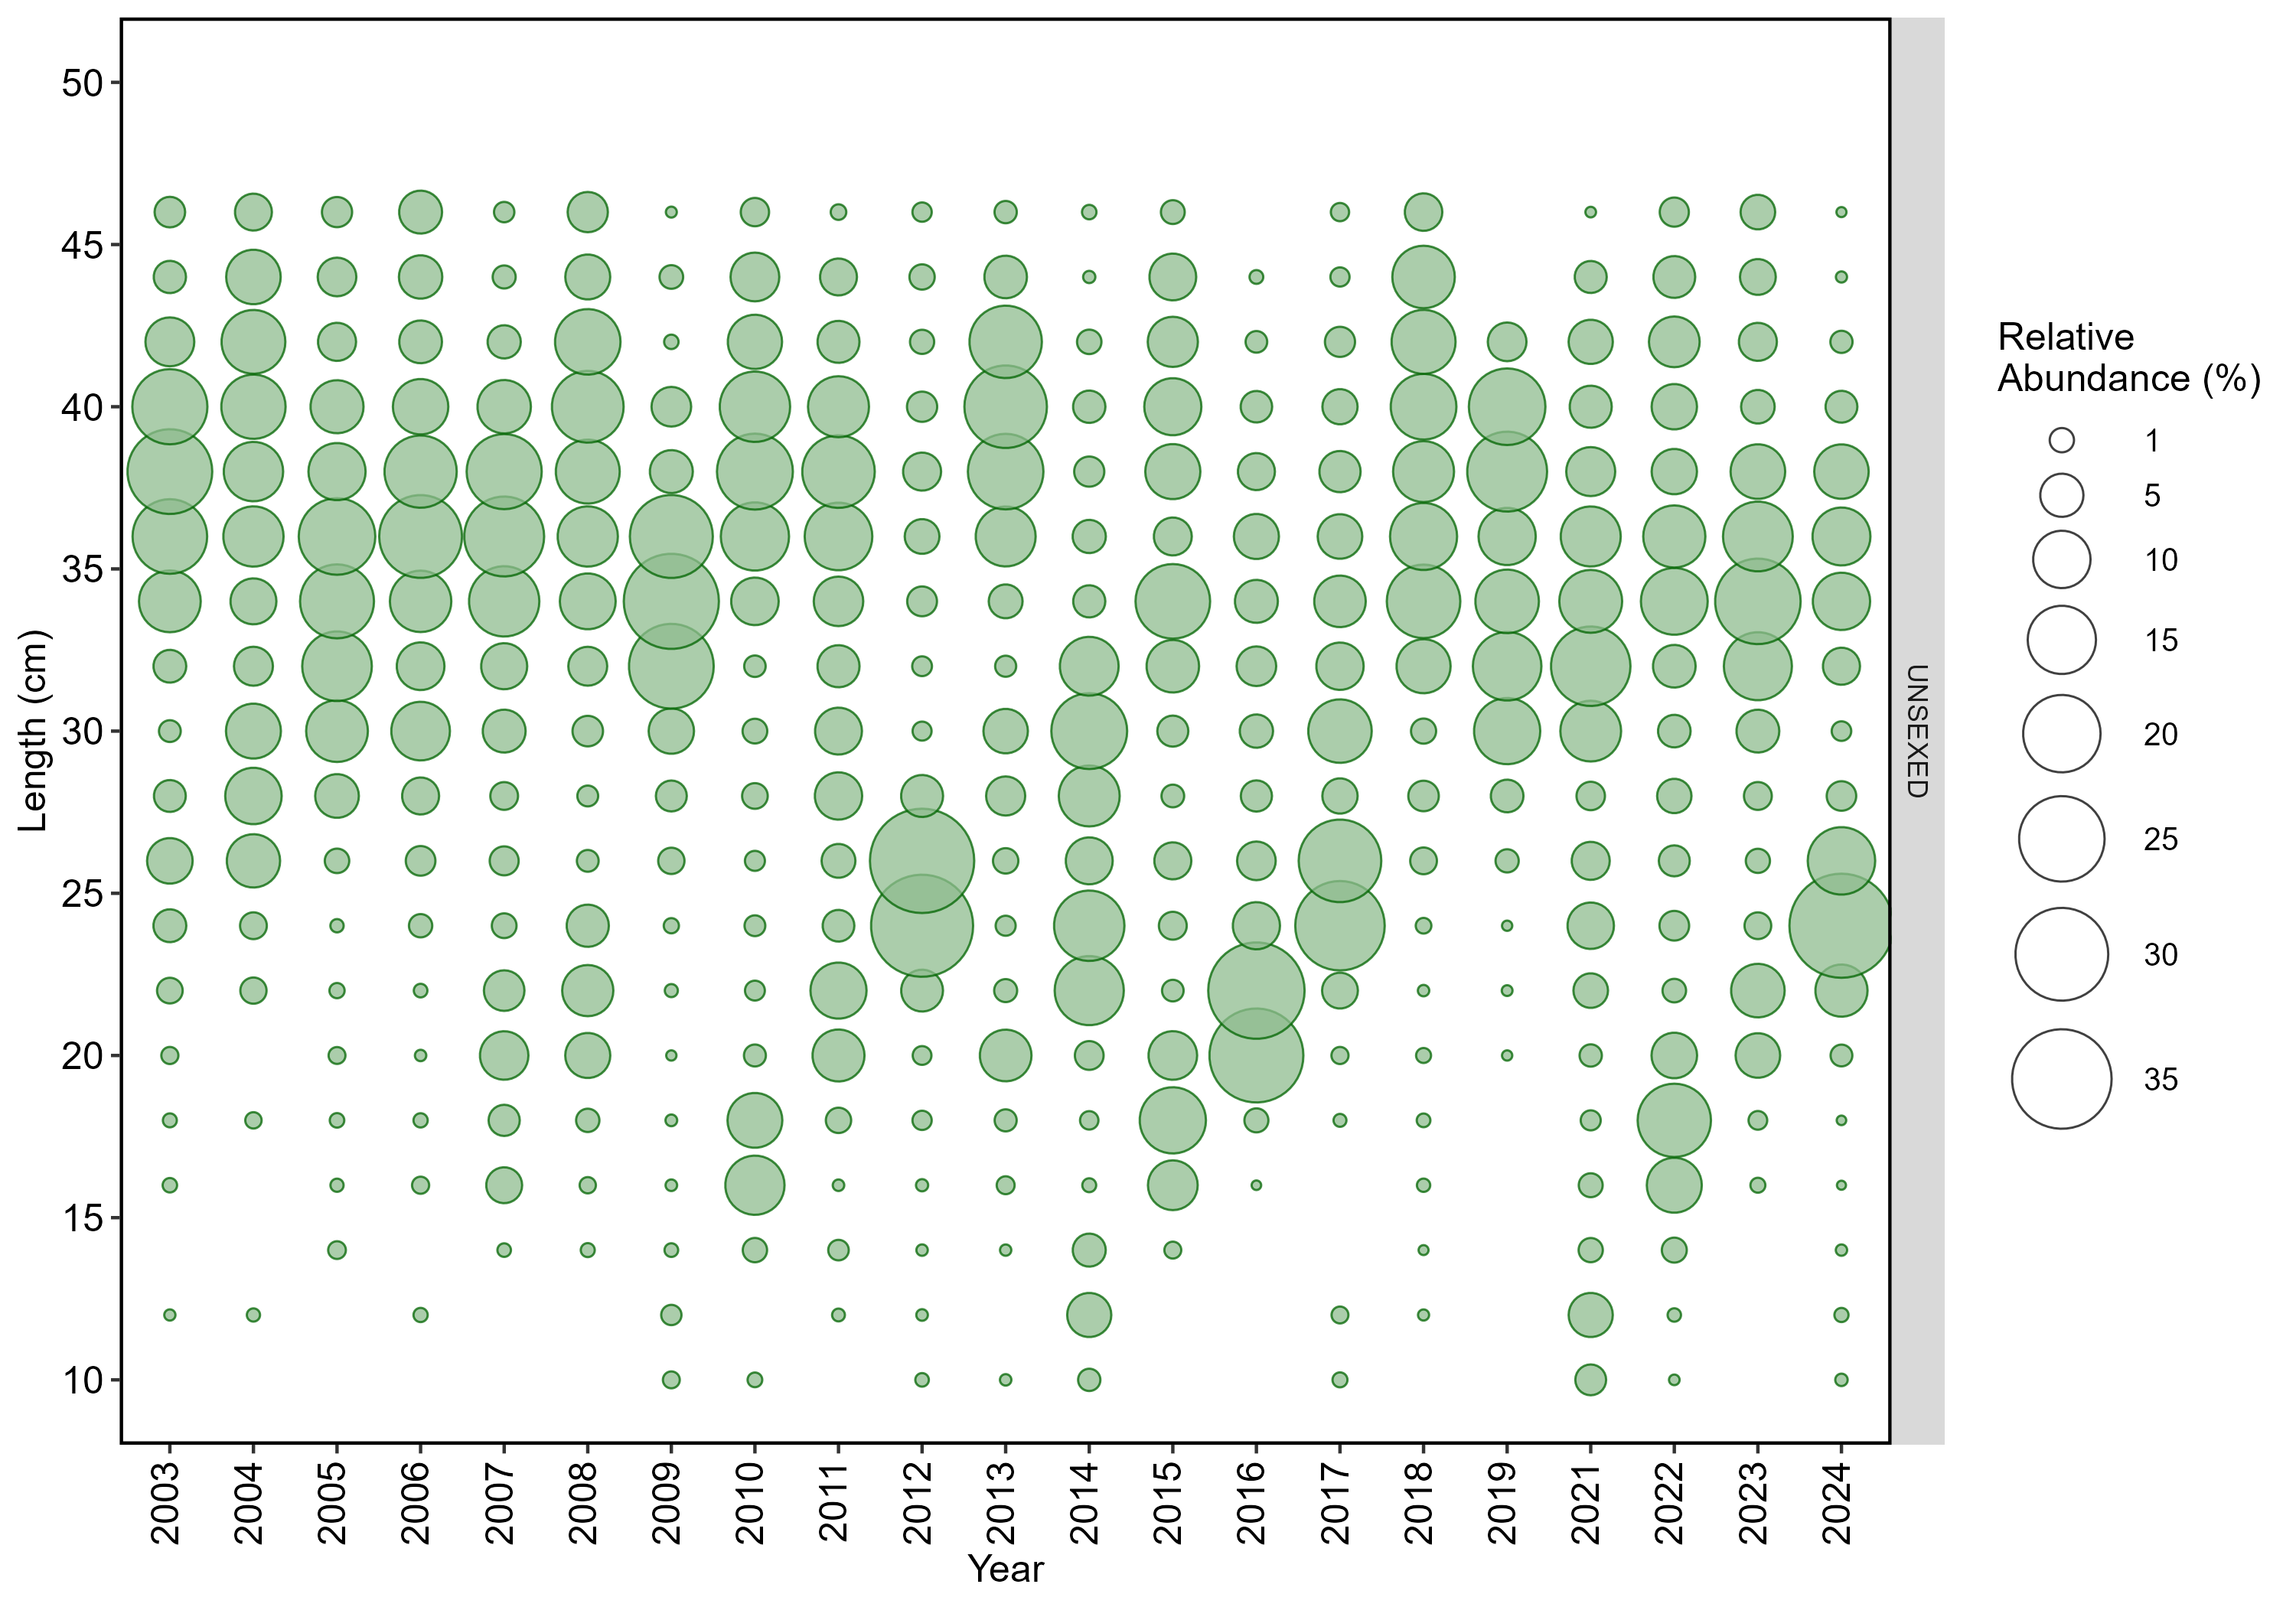
\includegraphics[width=0.95\linewidth,height=\textheight,keepaspectratio]{../plots/wcgbts_comps/plots/Pacific ocean perch_length_frequency_sex_0.png}

}

\caption{Length (cm) compostion data from the NWFSC WCGBTS for Pacific
ocean perch. Size of the circles within a year indicate higher (larger
circles) and lower (smaller circles) proportion observed by length bin.}

\end{figure}%

\newpage{}

\subsection{Pacific sanddab}\label{pacific-sanddab}

To date, no assessment or analysis has been conducted on Pacific
sanddab. Across available data, Pacific sanddab have been observed and
sampled by the NWFSC WCGBTS. The NWFSC WCGBTS observed Pacific sanddab
on an average of 209 tows per year. For this species, a total of 0
maturity samples have been collected coastwide (regardless of stock
area).

\begingroup\fontsize{10}{12}\selectfont
\begingroup\fontsize{10}{12}\selectfont

\begin{longtable}[t]{>{\raggedleft\arraybackslash}p{2cm}>{\raggedleft\arraybackslash}p{3.5cm}>{\raggedleft\arraybackslash}p{2cm}>{\raggedleft\arraybackslash}p{2cm}>{\raggedleft\arraybackslash}p{2cm}}
\caption{\label{tab:unnamed-chunk-397}Total number of available lengths, read ages, and unread age structures by data source and
state for Pacific sanddab.}\\
\toprule
State & Source & Lengths & Ages & Age Structures\\
\midrule
\endfirsthead
\caption[]{Total number of available lengths, read ages, and unread age structures by data source and
state for Pacific sanddab. (\textit{continued)}}\\
\toprule
State & Source & Lengths & Ages & Age Structures\\
\midrule
\endhead

\endfoot
\bottomrule
\endlastfoot
CA & NWFSC WCGBTS & 55,101 & 4,722 & 4,199\\
OR & NWFSC WCGBTS & 28,359 & 2,374 & 2,311\\
WA & NWFSC WCGBTS & 10,908 & 874 & 973\\*
\end{longtable}
\endgroup{}
\endgroup{}

\begin{figure}[H]

{\centering 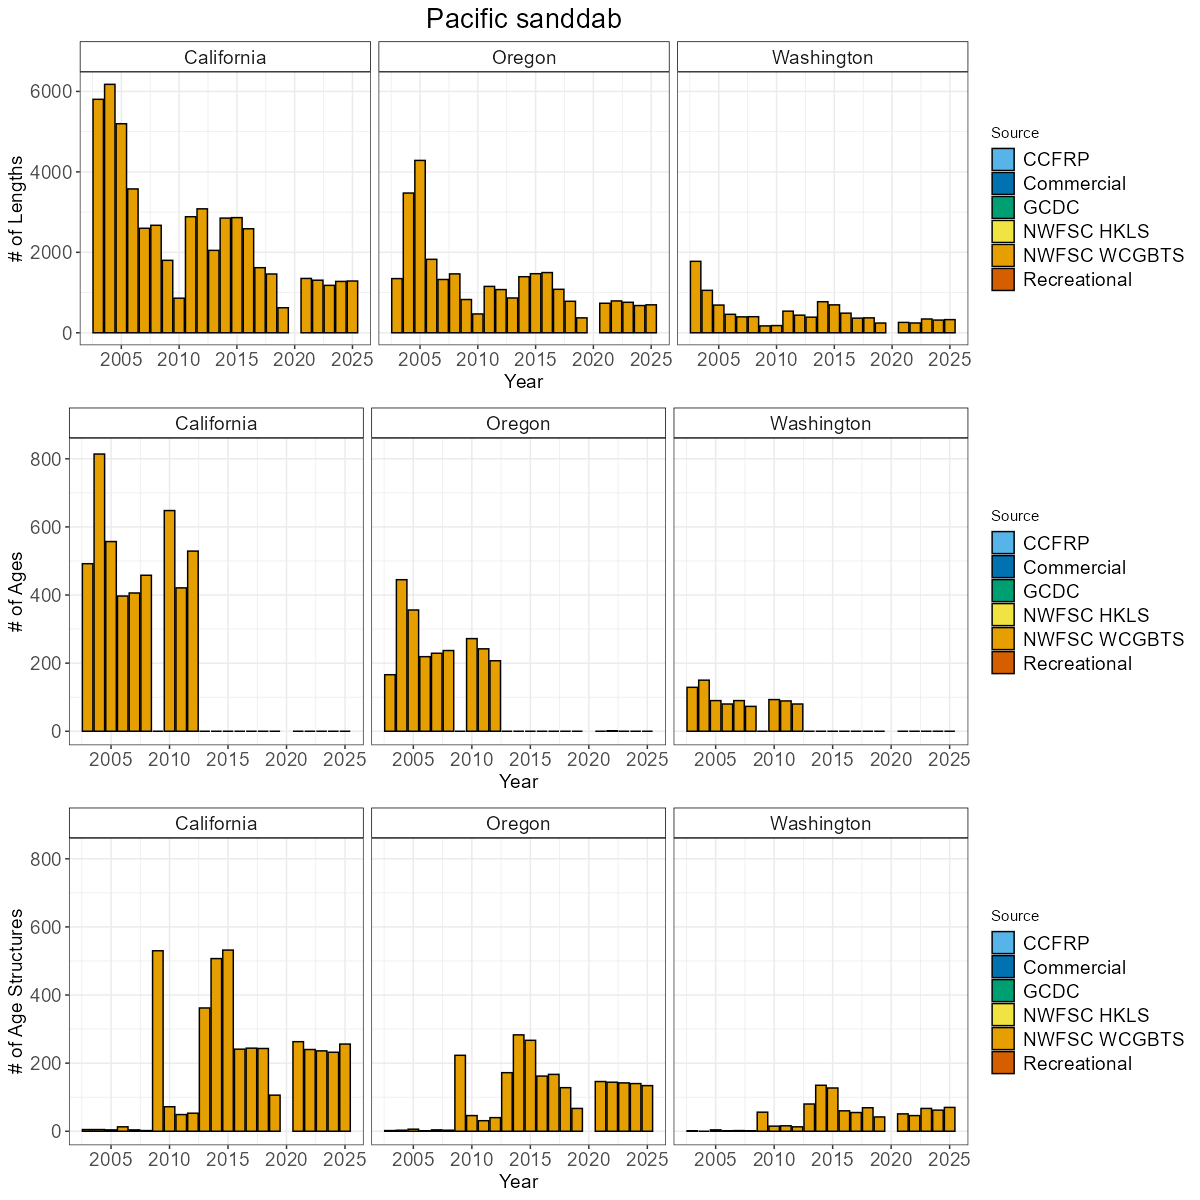
\includegraphics[width=0.95\linewidth,height=\textheight,keepaspectratio]{../plots/state_comparisons/pacific_sanddab_state_compositions.png}

}

\caption{Total number of available lengths, read ages, and unread age
structures by data source by year for Pacific sanddab. Note the y-axis
maximum may differ by data type.}

\end{figure}%

\begin{figure}[H]

{\centering 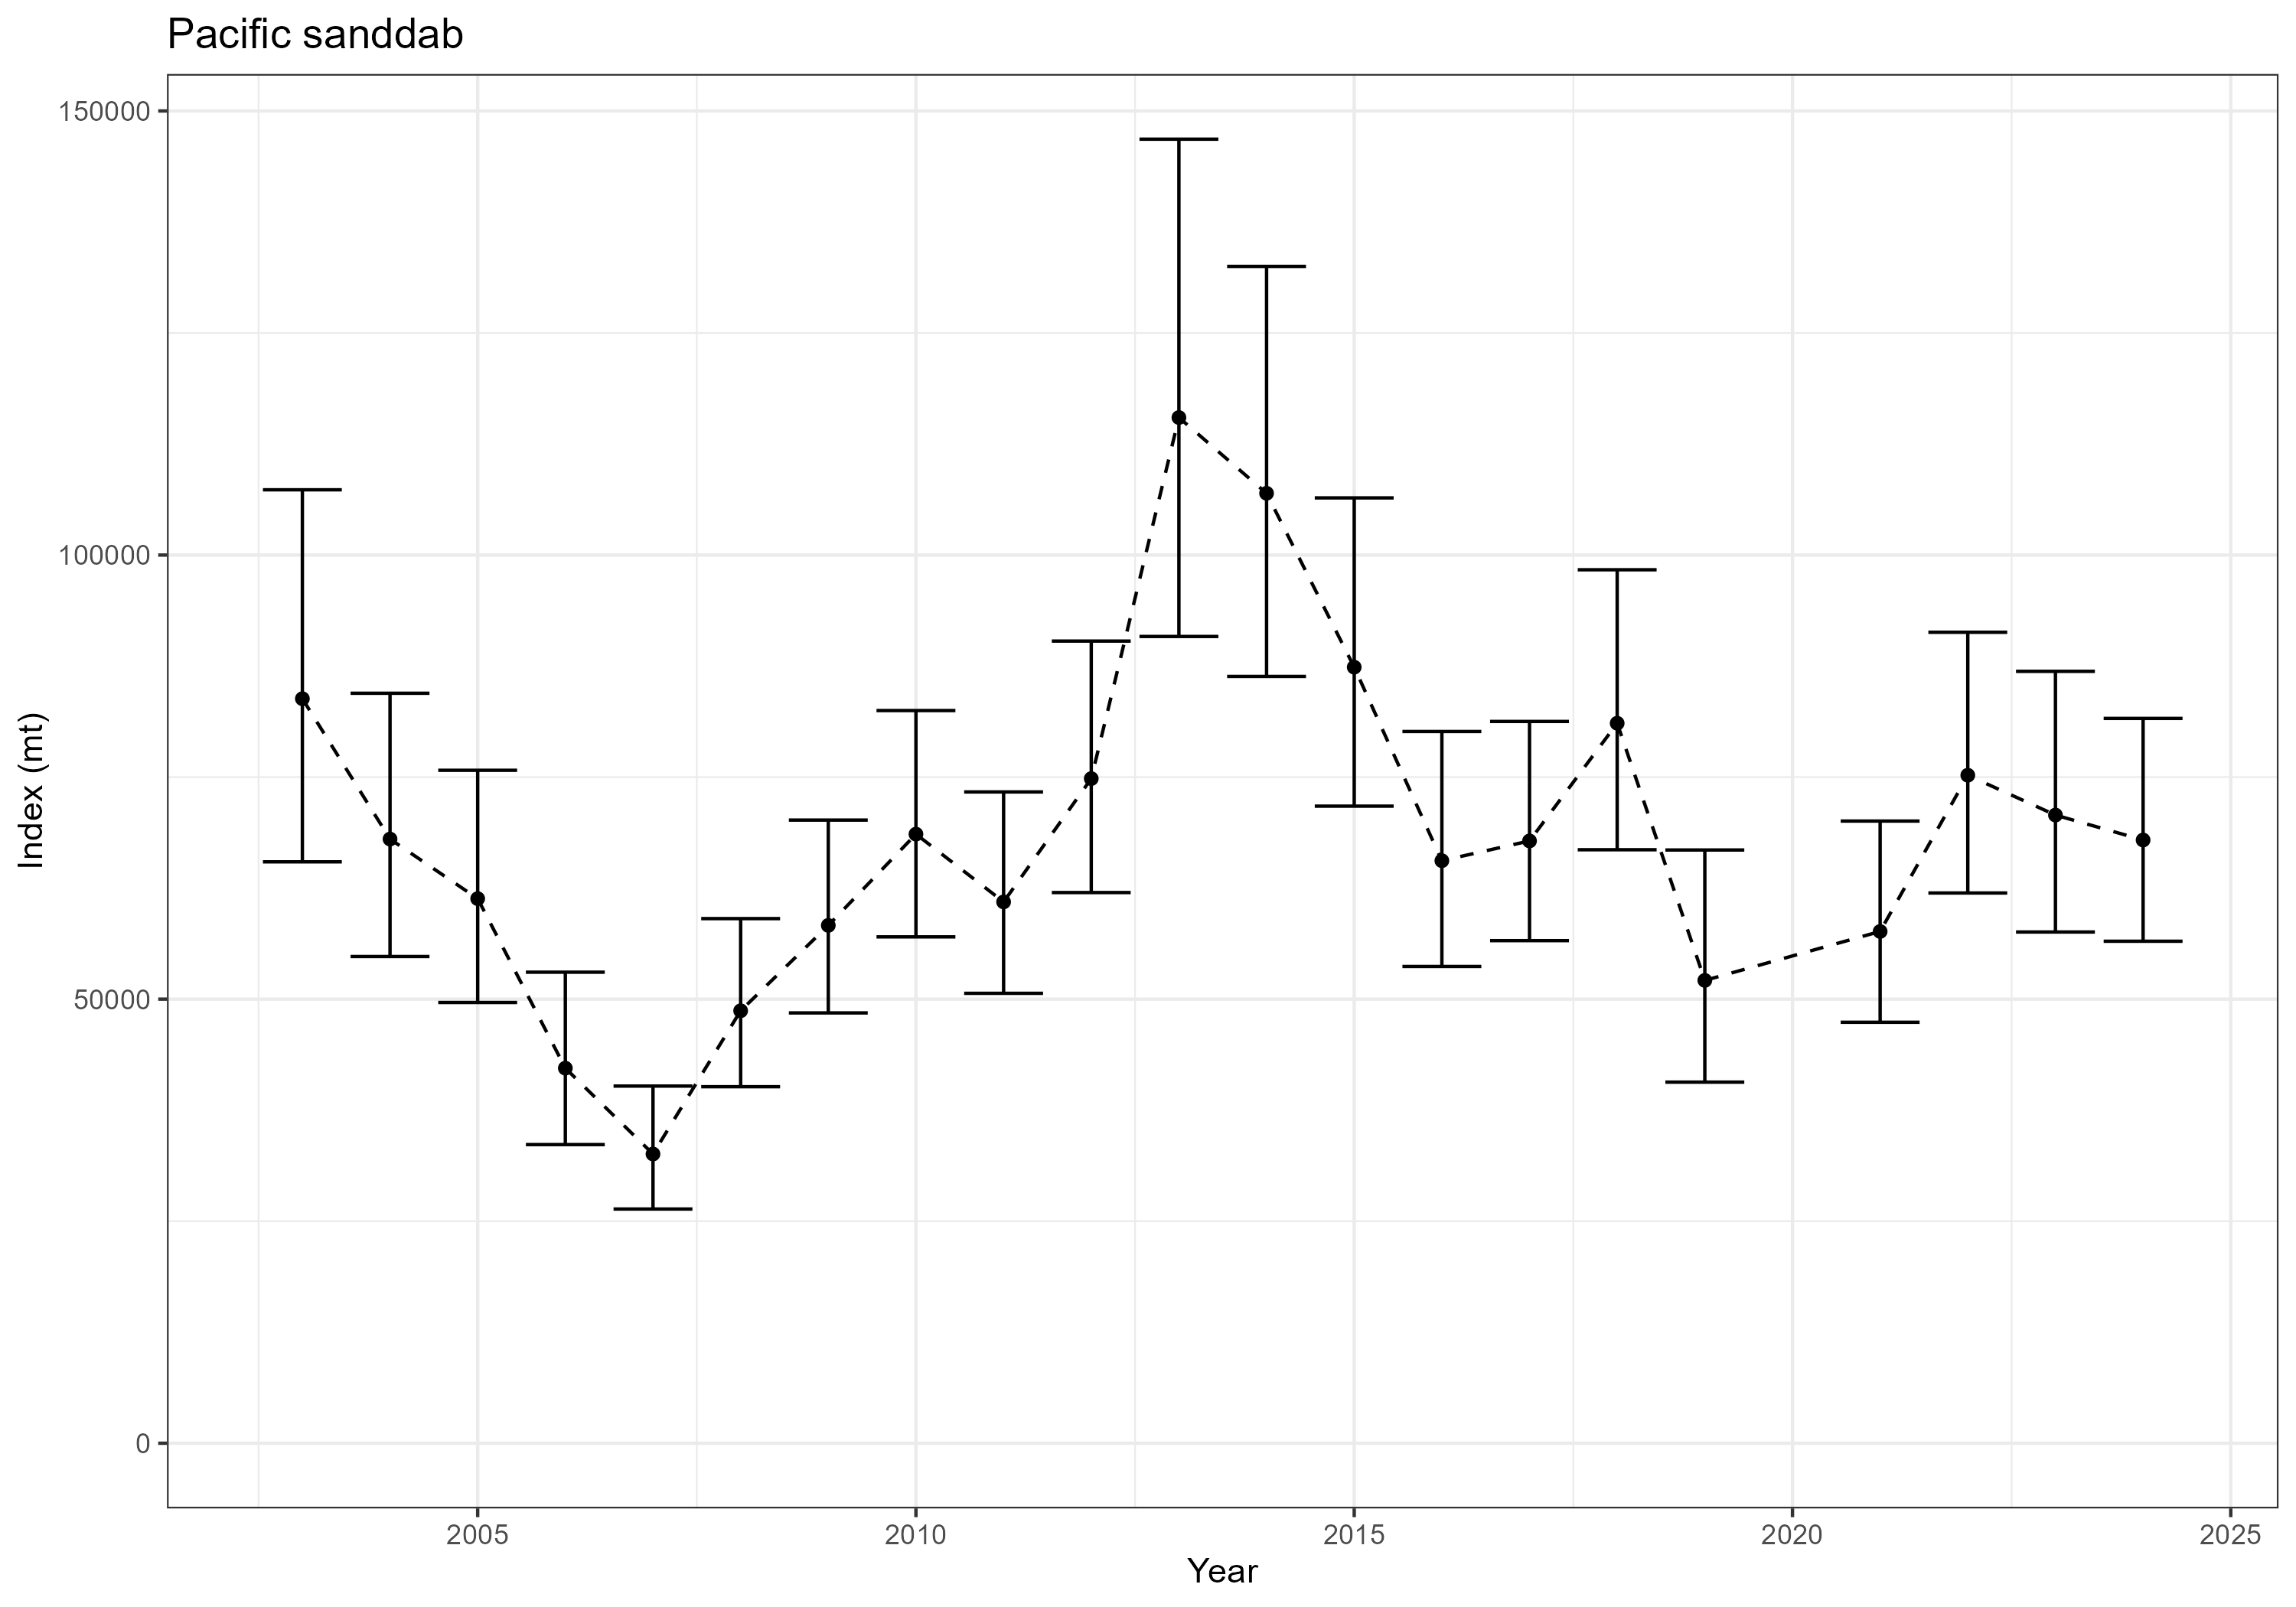
\includegraphics[width=0.95\linewidth,height=\textheight,keepaspectratio]{../plots/wcgbts_indices/pacific_sanddab_index.png}

}

\caption{Estimated relative index of abundance for Pacific sanddab from
the NWFSC WCGBTS.}

\end{figure}%

\begin{figure}[H]

{\centering 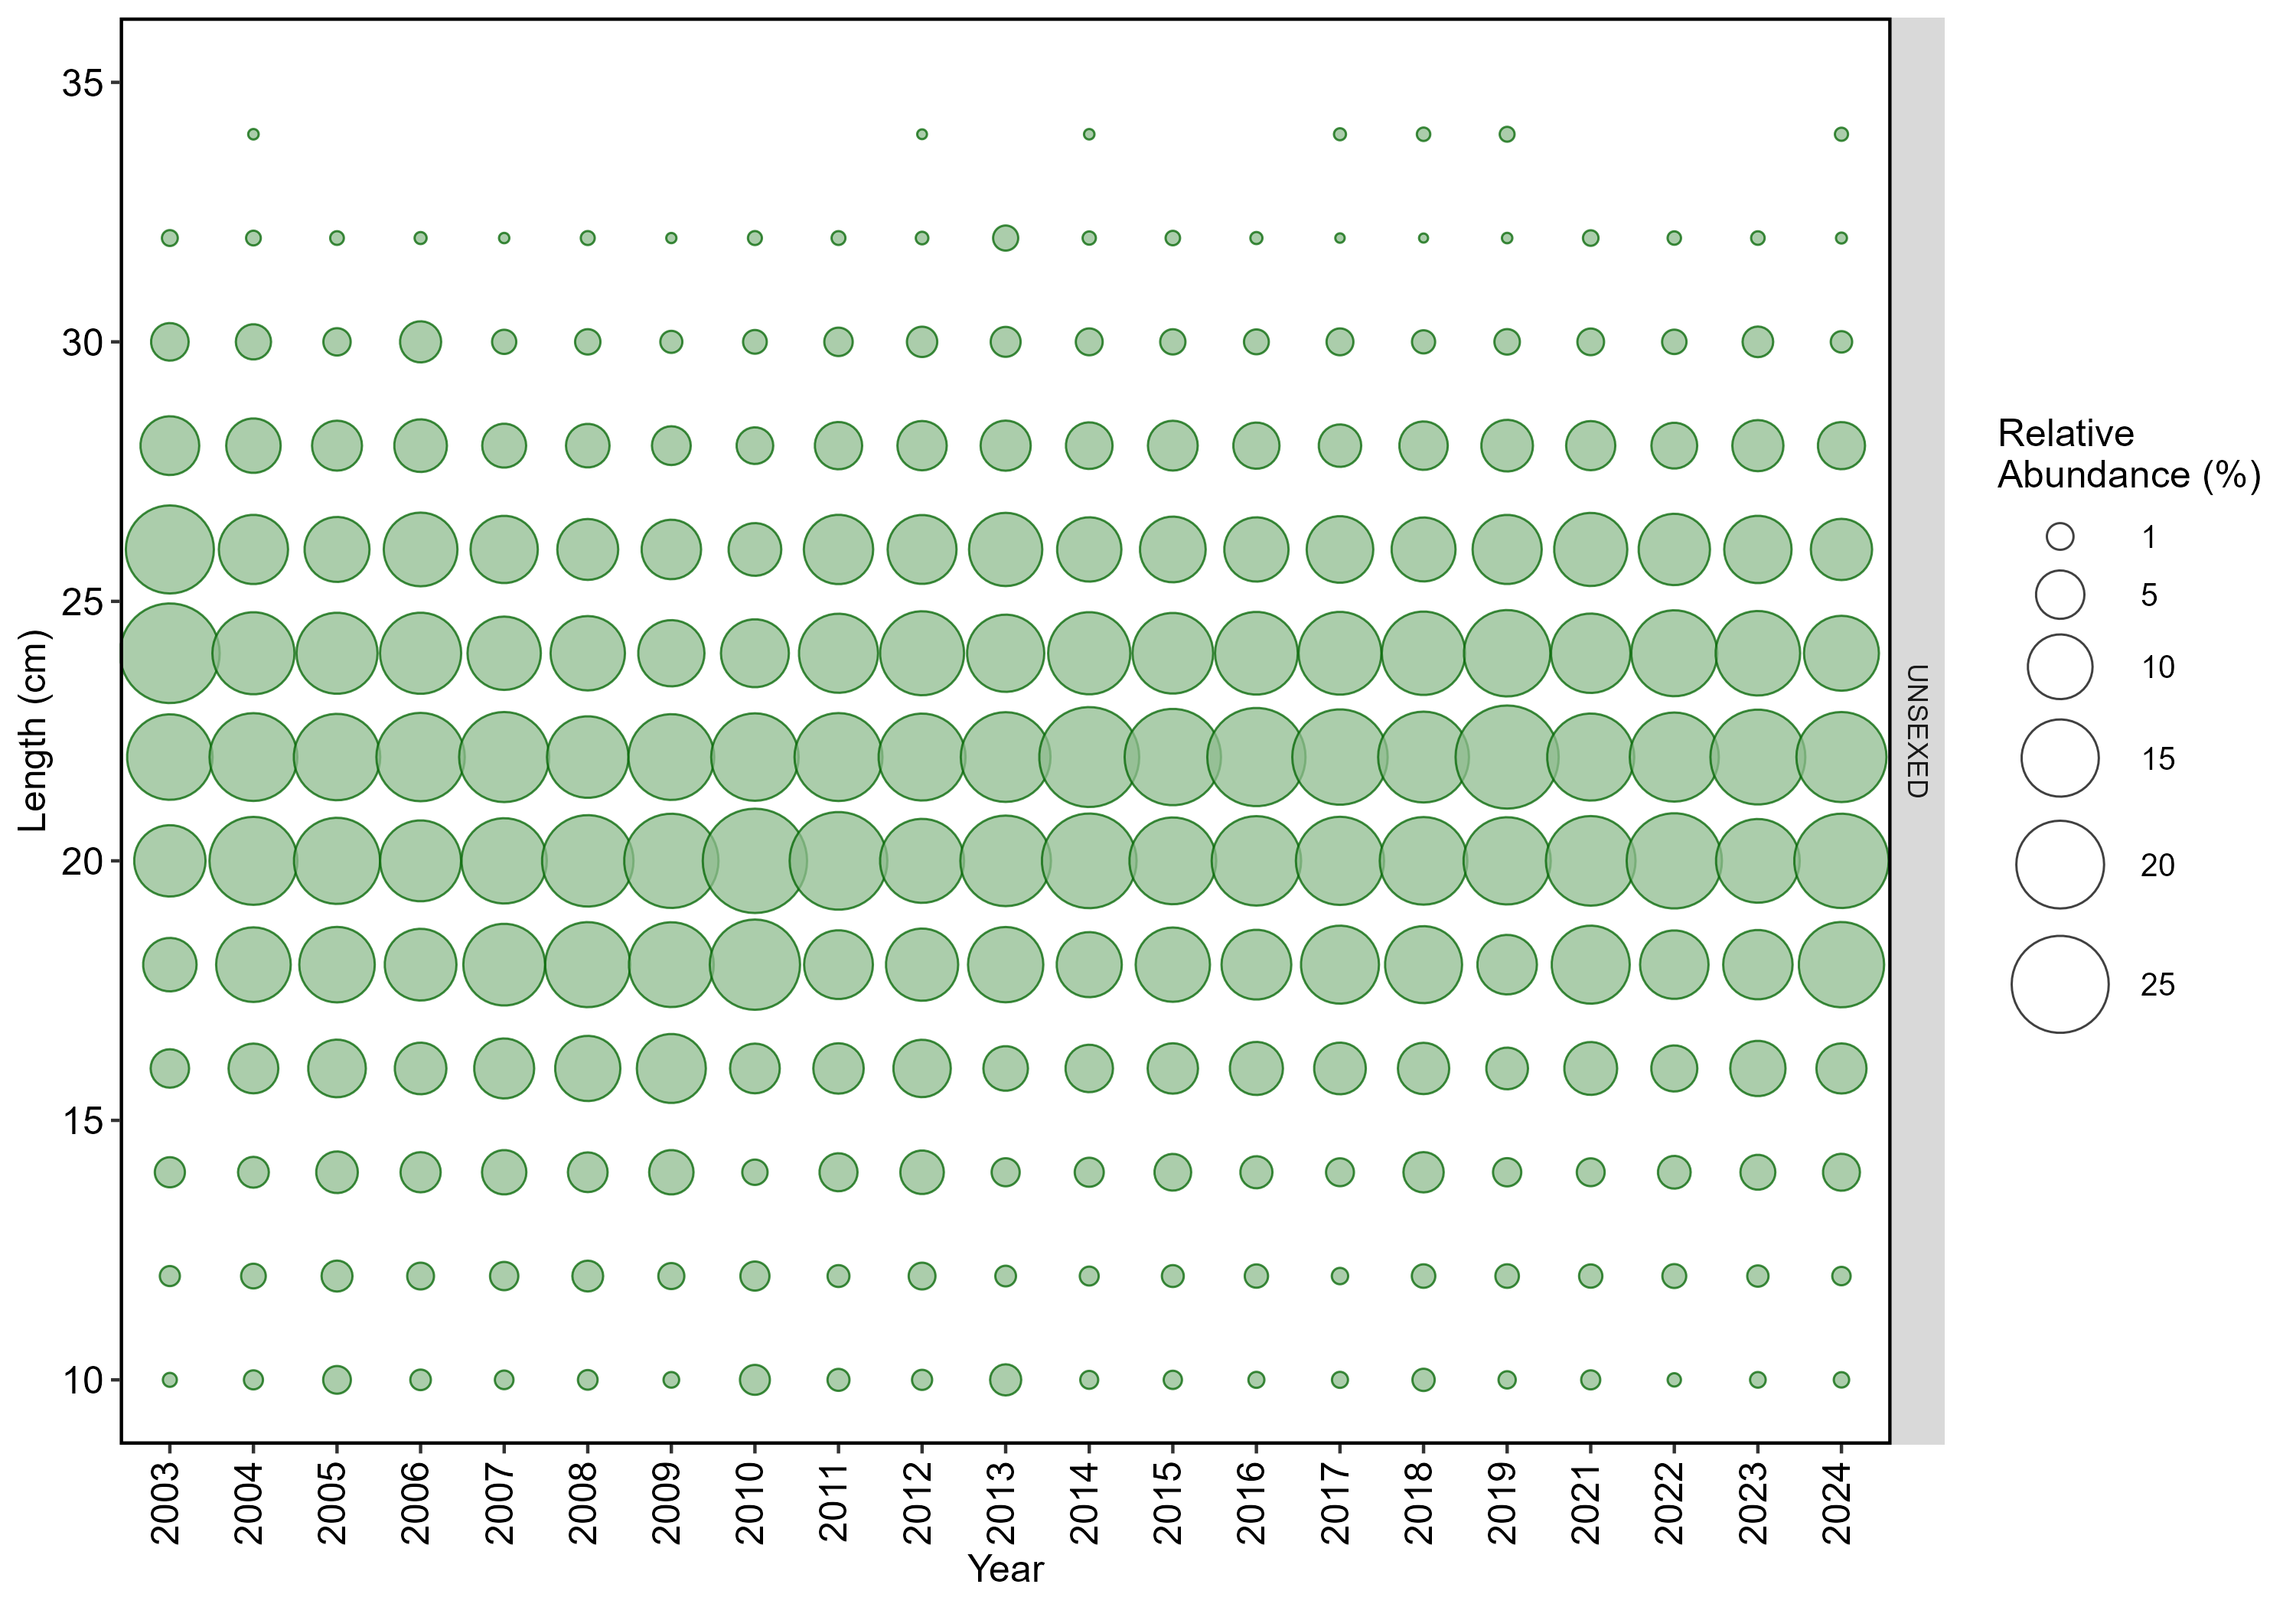
\includegraphics[width=0.95\linewidth,height=\textheight,keepaspectratio]{../plots/wcgbts_comps/plots/Pacific sanddab_length_frequency_sex_0.png}

}

\caption{Length (cm) compostion data from the NWFSC WCGBTS for Pacific
sanddab. Size of the circles within a year indicate higher (larger
circles) and lower (smaller circles) proportion observed by length bin.}

\end{figure}%

\newpage{}

\subsection{Pacific spiny dogfish}\label{pacific-spiny-dogfish}

The most recent assessment of Pacific spiny dogfish was a benchmark
assessment conducted in 2021. Across available data, Pacific spiny
dogfish have been observed and sampled by both the NWFSC HKLS and
WCGBTS. The NWFSC HKLS observed Pacific spiny dogfish at an average of 0
sets per year. The NWFSC WCGBTS observed Pacific spiny dogfish on an
average of 161 tows per year. For this species, a total of 0 maturity
samples have been collected coastwide (regardless of stock area).
Researchers have conducted an analysis of the trends of Pacific spiny
dogfish across the North Pacific indicating declining population trends
across regions.

\begingroup\fontsize{10}{12}\selectfont
\begingroup\fontsize{10}{12}\selectfont

\begin{longtable}[t]{>{\raggedleft\arraybackslash}p{2cm}>{\raggedleft\arraybackslash}p{3.5cm}>{\raggedleft\arraybackslash}p{2cm}>{\raggedleft\arraybackslash}p{2cm}>{\raggedleft\arraybackslash}p{2cm}}
\caption{\label{tab:unnamed-chunk-414}Total number of available lengths, read ages, and unread age structures by data source and
state for Pacific spiny dogfish.}\\
\toprule
State & Source & Lengths & Ages & Age Structures\\
\midrule
\endfirsthead
\caption[]{Total number of available lengths, read ages, and unread age structures by data source and
state for Pacific spiny dogfish. (\textit{continued)}}\\
\toprule
State & Source & Lengths & Ages & Age Structures\\
\midrule
\endhead

\endfoot
\bottomrule
\endlastfoot
CA & NWFSC HKLS & 9 & 0 & 0\\
CA & NWFSC WCGBTS & 18,373 & 285 & 4,941\\
OR & NWFSC WCGBTS & 4,454 & 128 & 1,925\\
WA & NWFSC WCGBTS & 11,802 & 178 & 2,972\\*
\end{longtable}
\endgroup{}
\endgroup{}

\begin{figure}[H]

{\centering 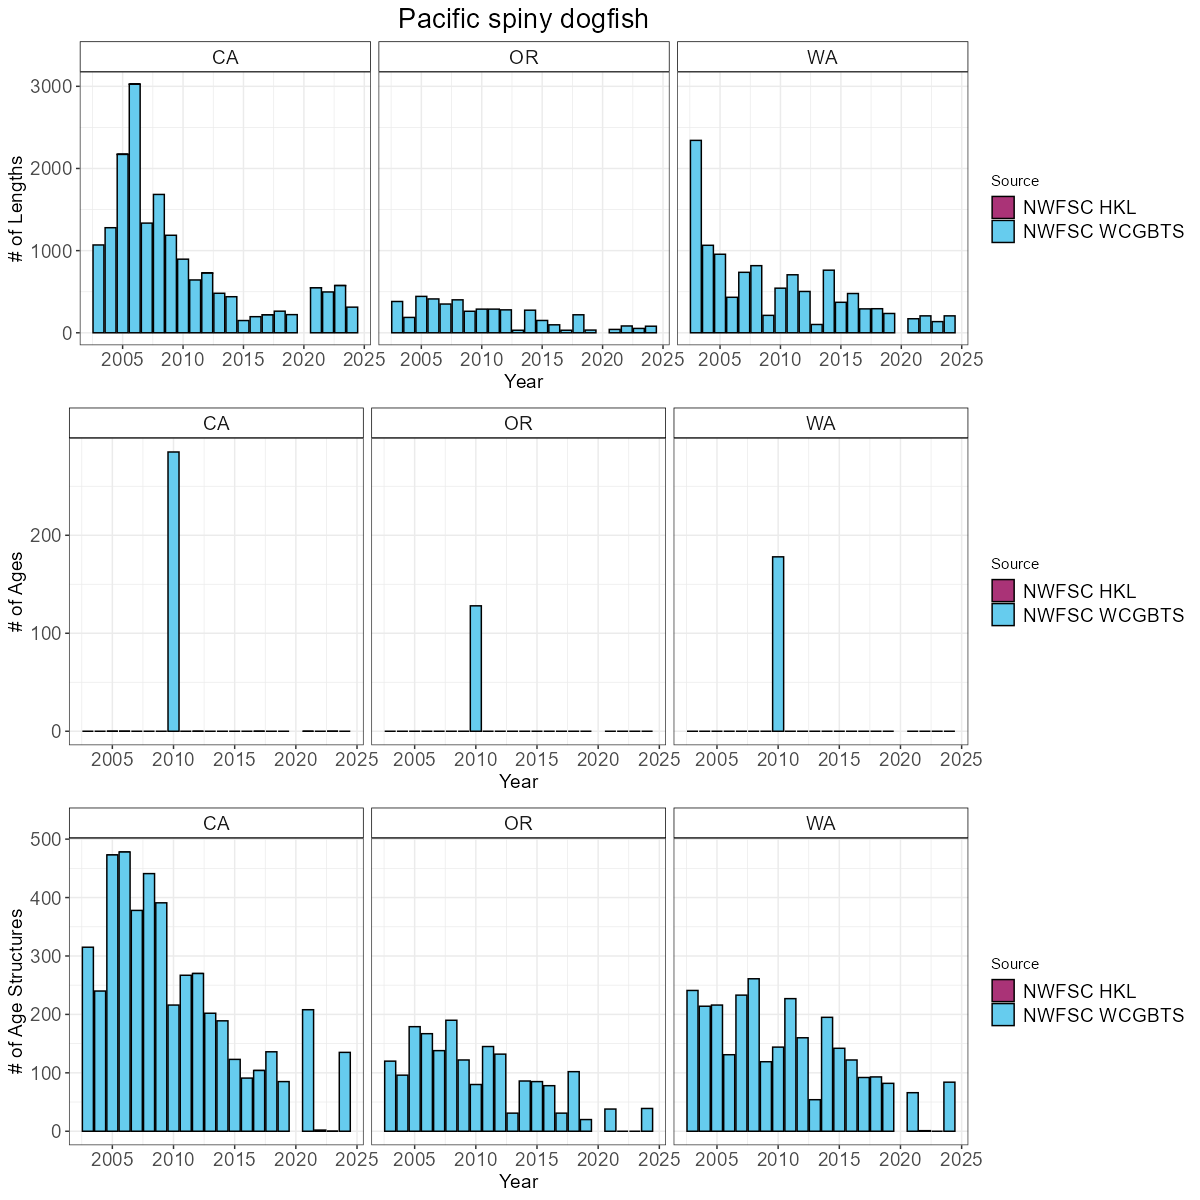
\includegraphics[width=0.95\linewidth,height=\textheight,keepaspectratio]{../plots/state_comparisons/pacific_spiny_dogfish_state_compositions.png}

}

\caption{Total number of available lengths, read ages, and unread age
structures by data source by year for Pacific spiny dogfish. Note the
y-axis maximum may differ by data type.}

\end{figure}%

\begin{figure}[H]

{\centering 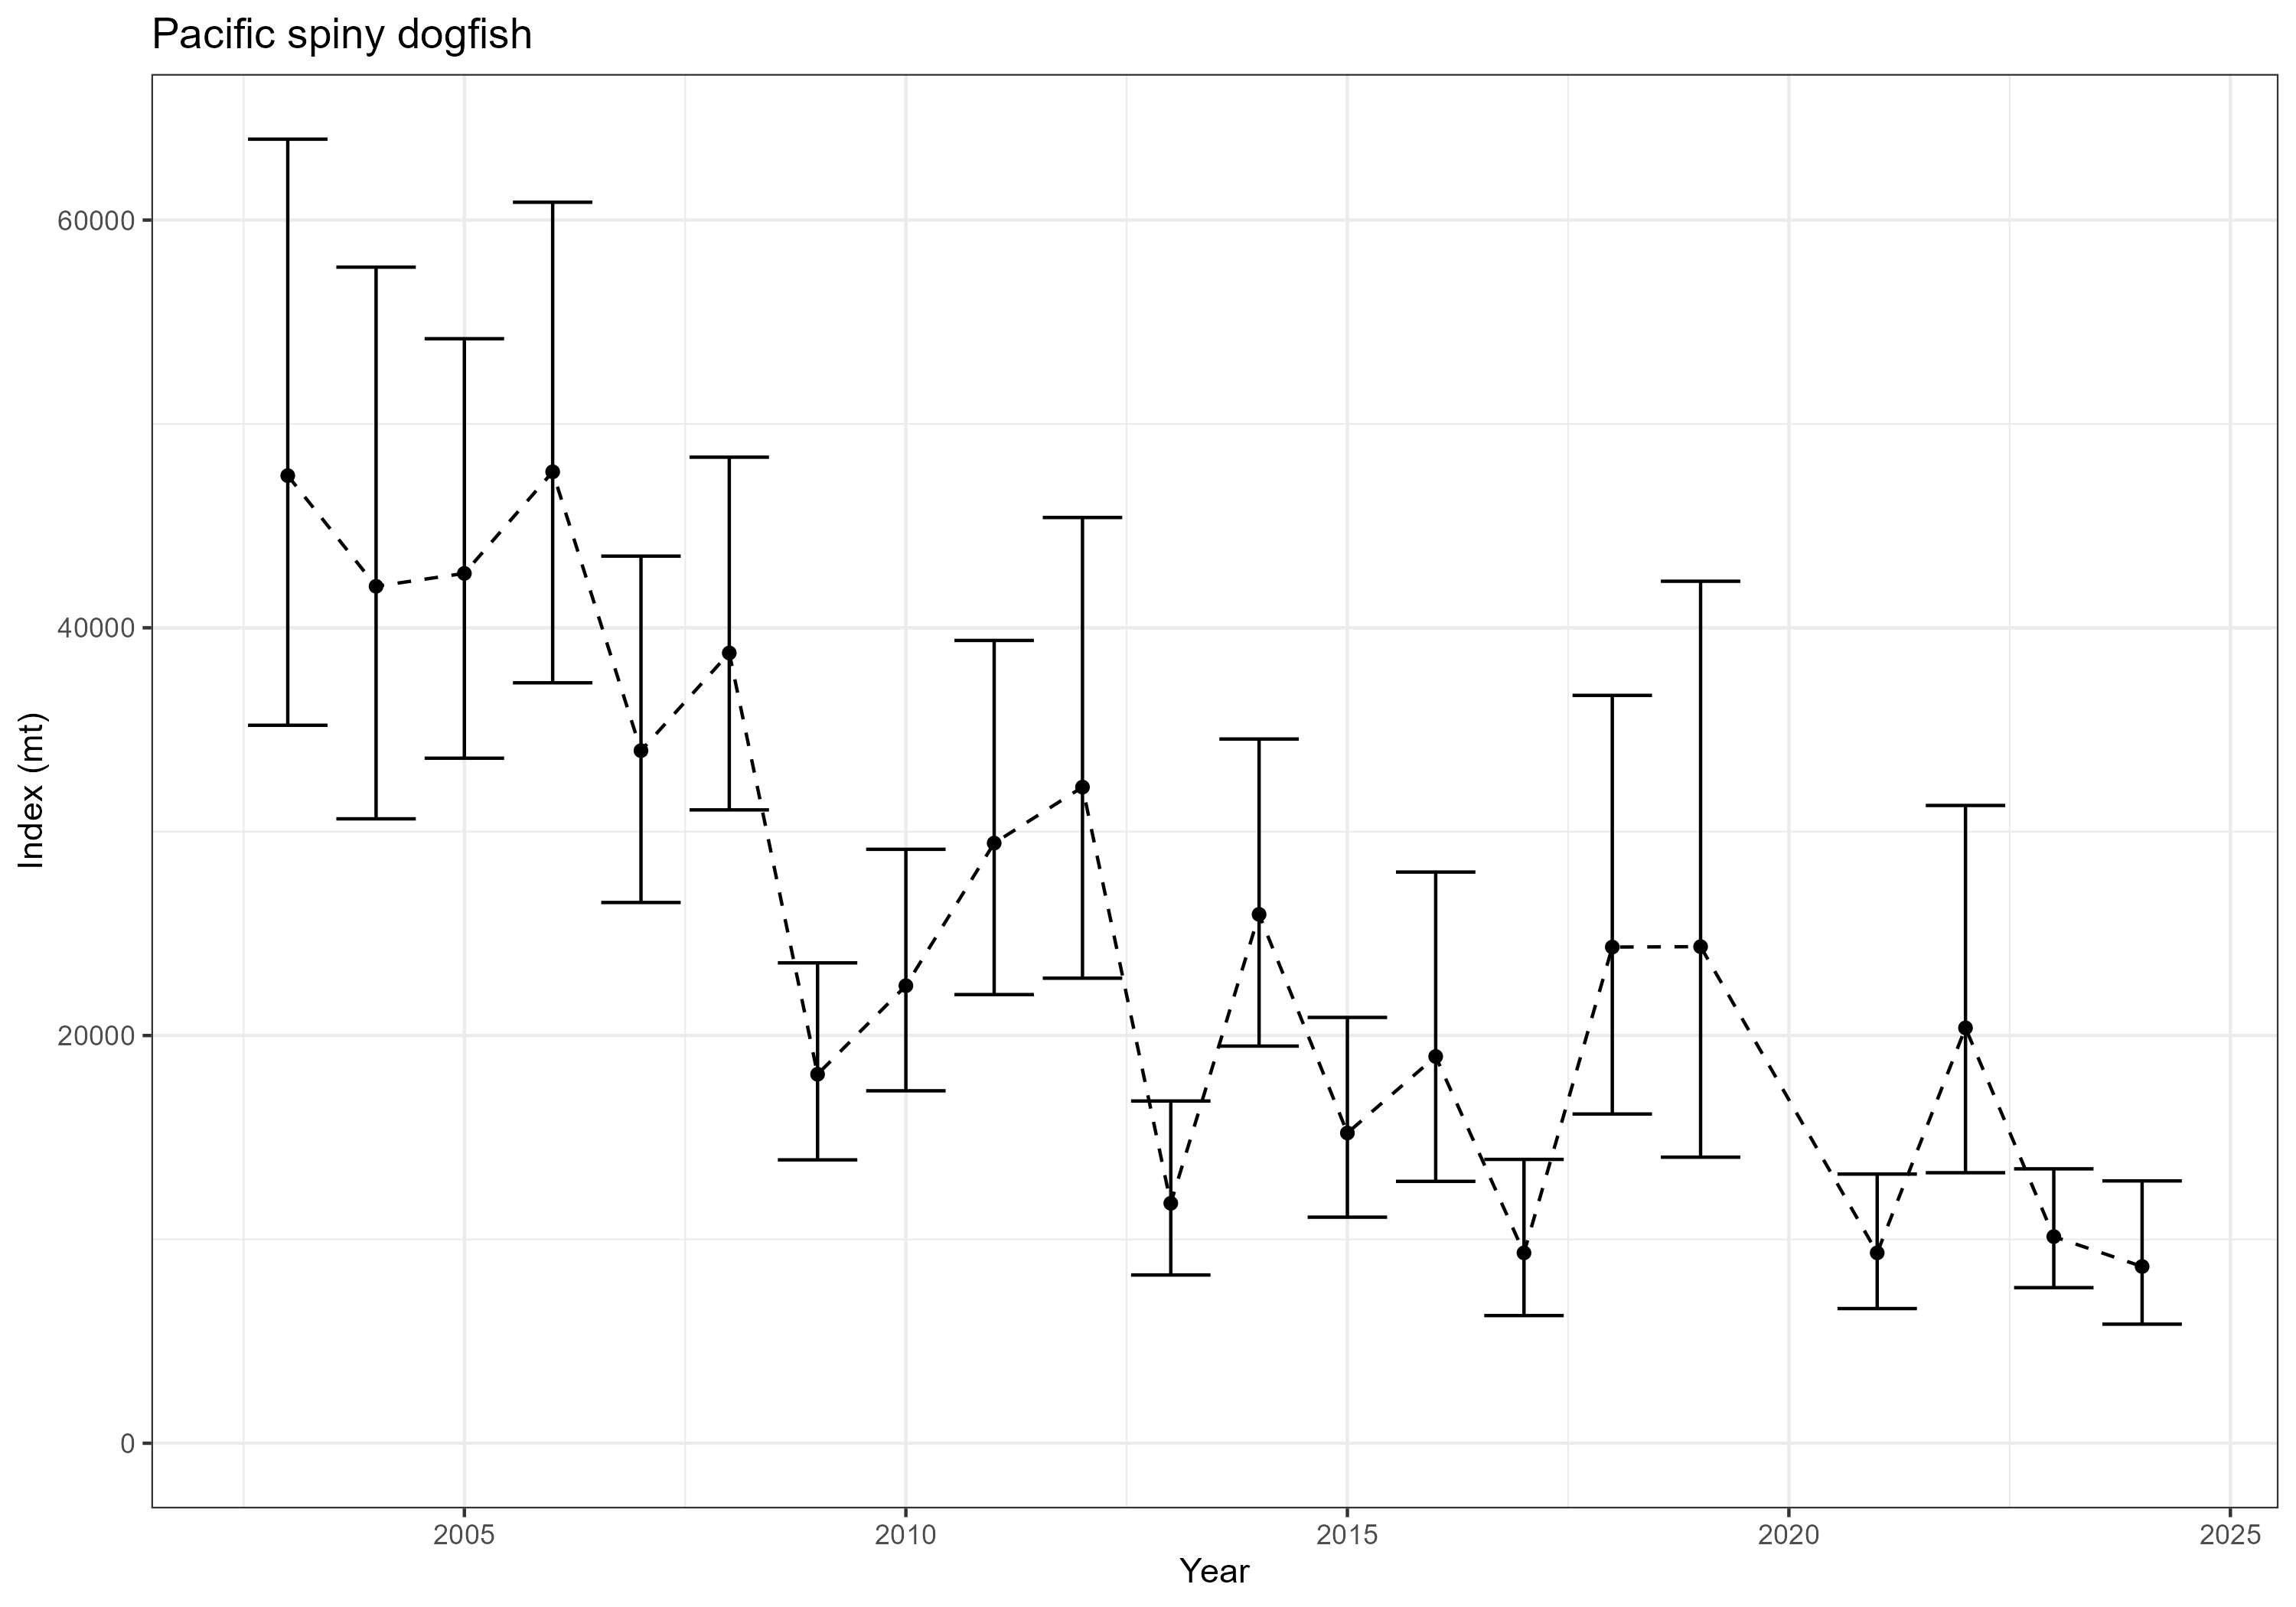
\includegraphics[width=0.95\linewidth,height=\textheight,keepaspectratio]{../plots/wcgbts_indices/pacific_spiny_dogfish_index.png}

}

\caption{Estimated relative index of abundance for Pacific spiny dogfish
from the NWFSC WCGBTS.}

\end{figure}%

\begin{figure}[H]

{\centering 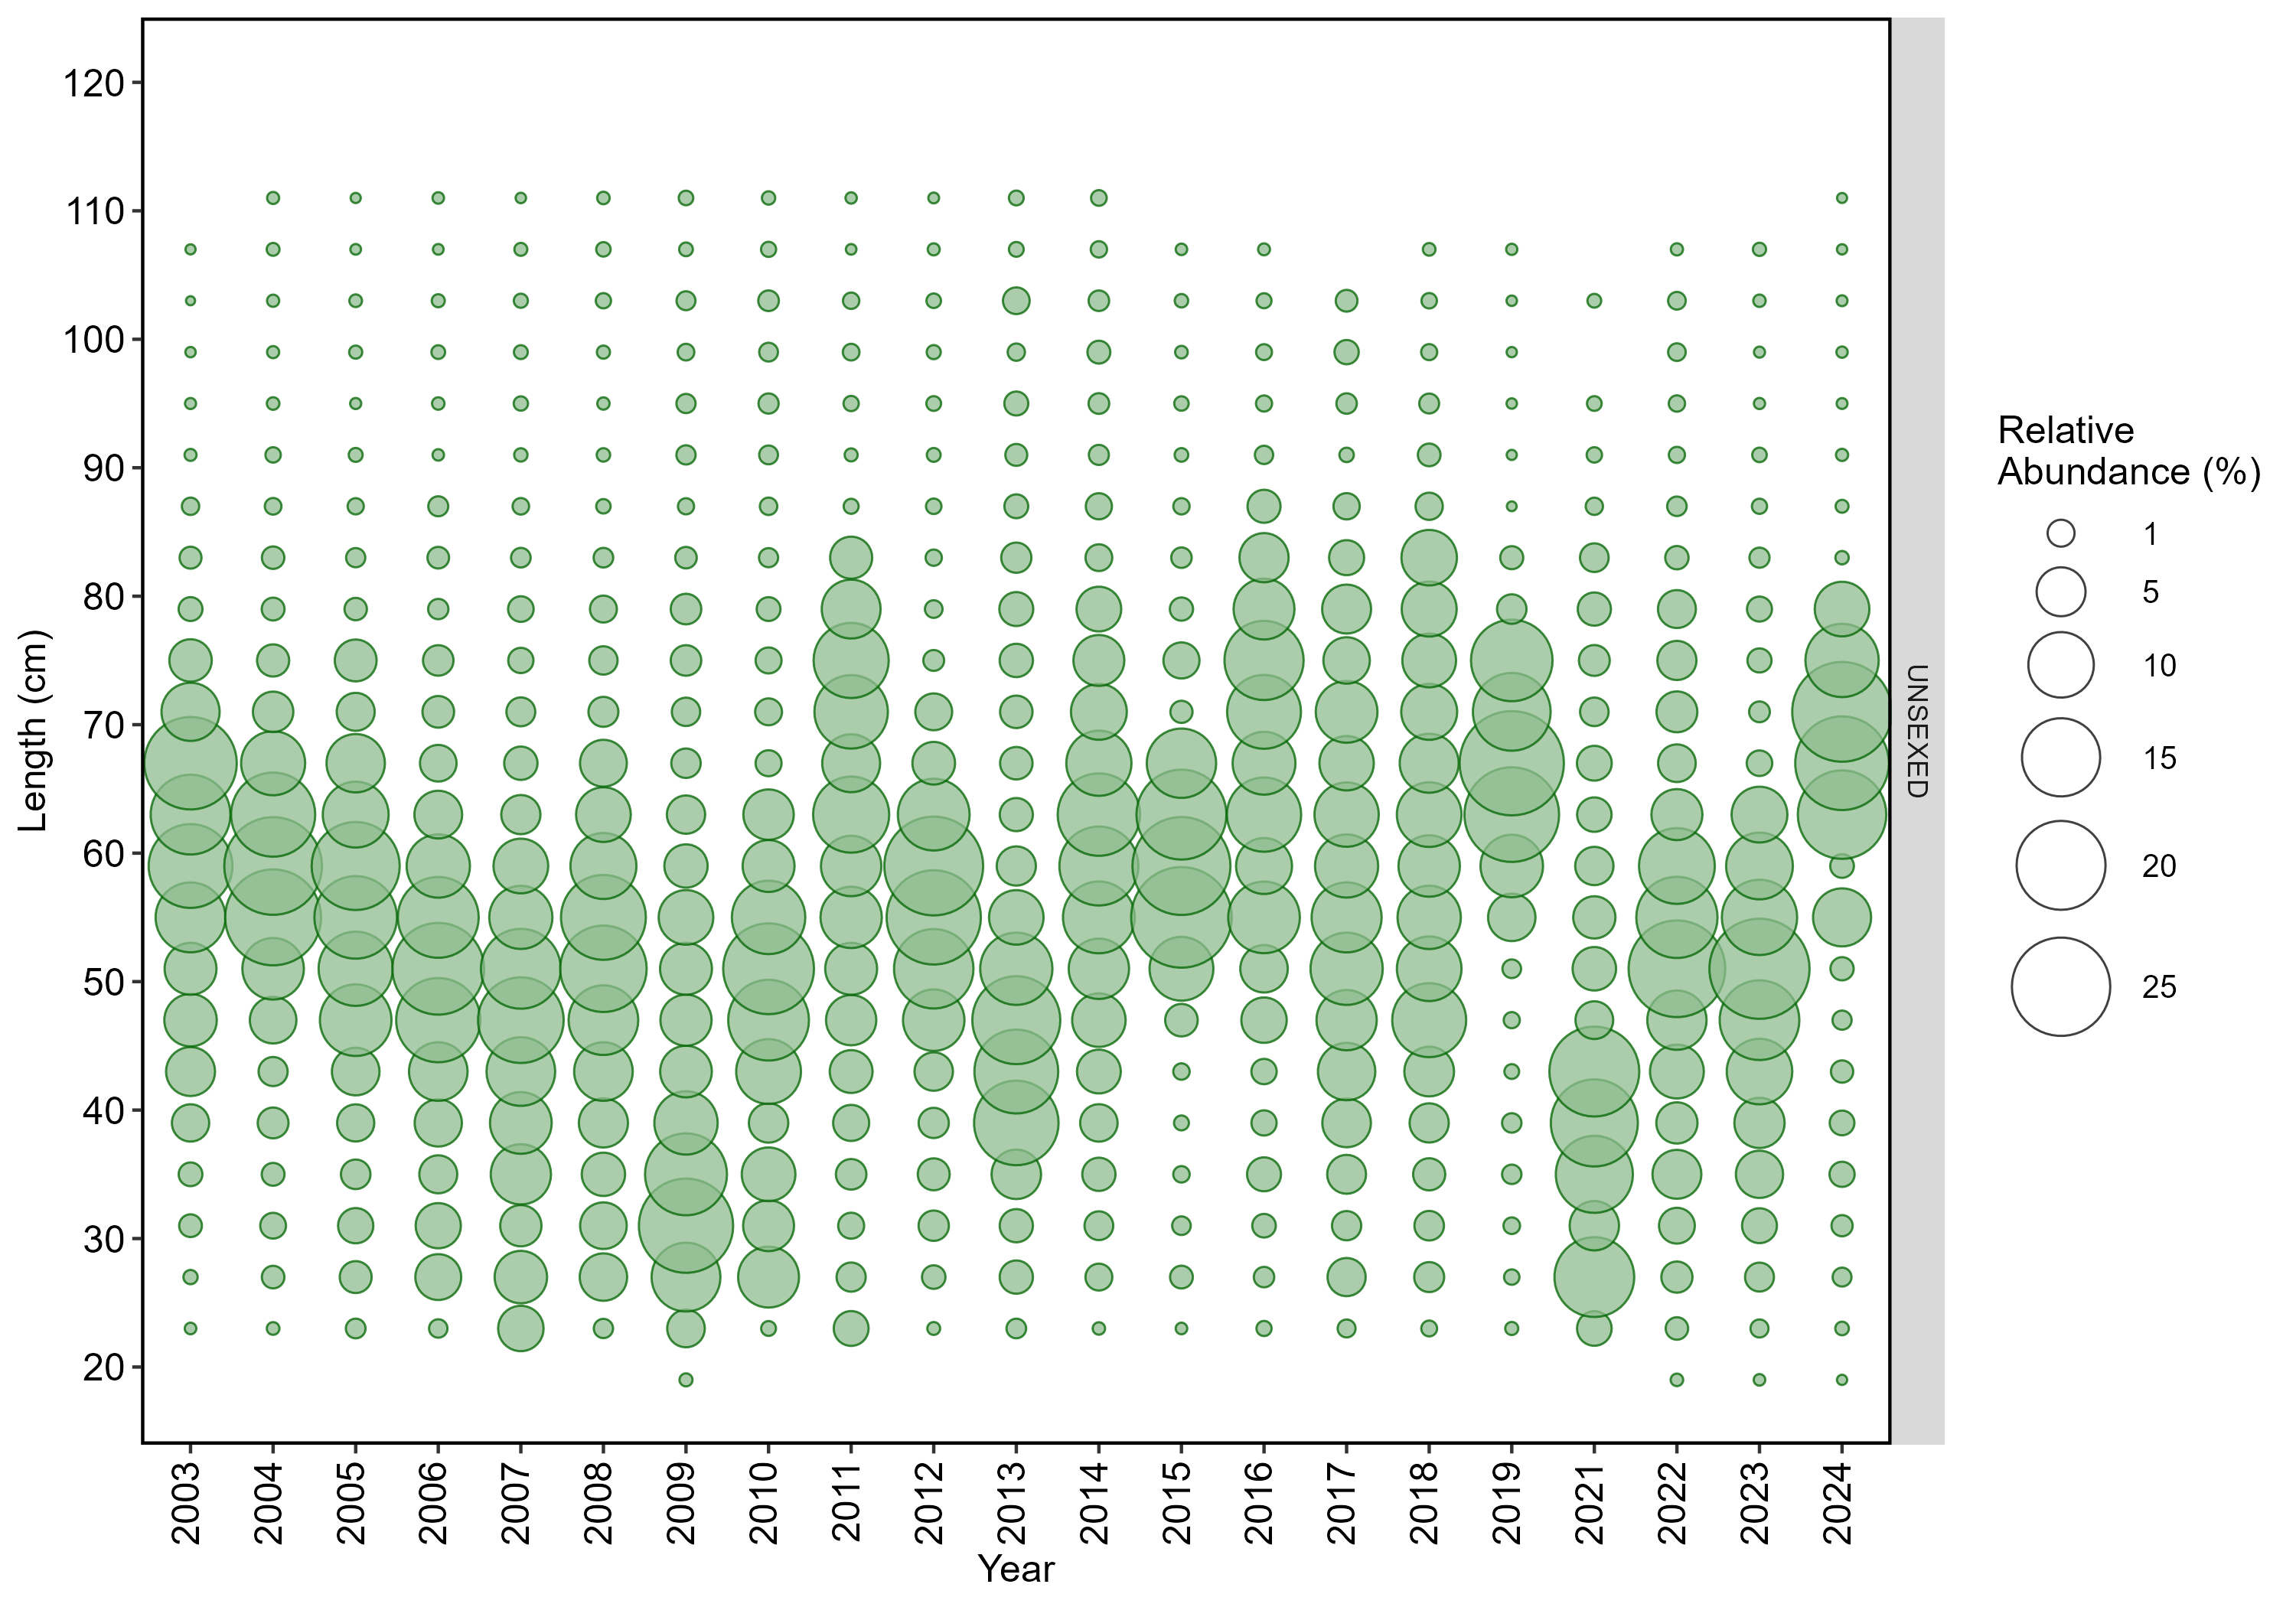
\includegraphics[width=0.95\linewidth,height=\textheight,keepaspectratio]{../plots/wcgbts_comps/plots/Pacific spiny dogfish_length_frequency_sex_0.png}

}

\caption{Length (cm) compostion data from the NWFSC WCGBTS for Pacific
spiny dogfish. Size of the circles within a year indicate higher (larger
circles) and lower (smaller circles) proportion observed by length bin.}

\end{figure}%

\newpage{}

\subsection{Petrale sole}\label{petrale-sole}

The most recent assessment of petrale sole was a benchmark assessment
conducted in 2023. Across available data, petrale sole have been
observed and sampled by both the NWFSC HKLS and WCGBTS. The NWFSC HKLS
observed petrale sole at an average of 0 sets per year. The NWFSC WCGBTS
observed petrale sole on an average of 275 tows per year. For this
species, a total of 728 maturity samples have been collected coastwide
(regardless of stock area), with 598 read maturities.

\begingroup\fontsize{10}{12}\selectfont
\begingroup\fontsize{10}{12}\selectfont

\begin{longtable}[t]{>{\raggedleft\arraybackslash}p{2cm}>{\raggedleft\arraybackslash}p{3.5cm}>{\raggedleft\arraybackslash}p{2cm}>{\raggedleft\arraybackslash}p{2cm}>{\raggedleft\arraybackslash}p{2cm}}
\caption{\label{tab:unnamed-chunk-431}Total number of available lengths, read ages, and unread age structures by data source and
state for petrale sole.}\\
\toprule
State & Source & Lengths & Ages & Age Structures\\
\midrule
\endfirsthead
\caption[]{Total number of available lengths, read ages, and unread age structures by data source and
state for petrale sole. (\textit{continued)}}\\
\toprule
State & Source & Lengths & Ages & Age Structures\\
\midrule
\endhead

\endfoot
\bottomrule
\endlastfoot
CA & NWFSC HKLS & 8 & 0 & 0\\
CA & NWFSC WCGBTS & 37,567 & 7,176 & 3,384\\
OR & NWFSC WCGBTS & 33,022 & 4,860 & 3,910\\
WA & NWFSC WCGBTS & 16,233 & 2,676 & 2,272\\*
\end{longtable}
\endgroup{}
\endgroup{}

\begin{figure}[H]

{\centering 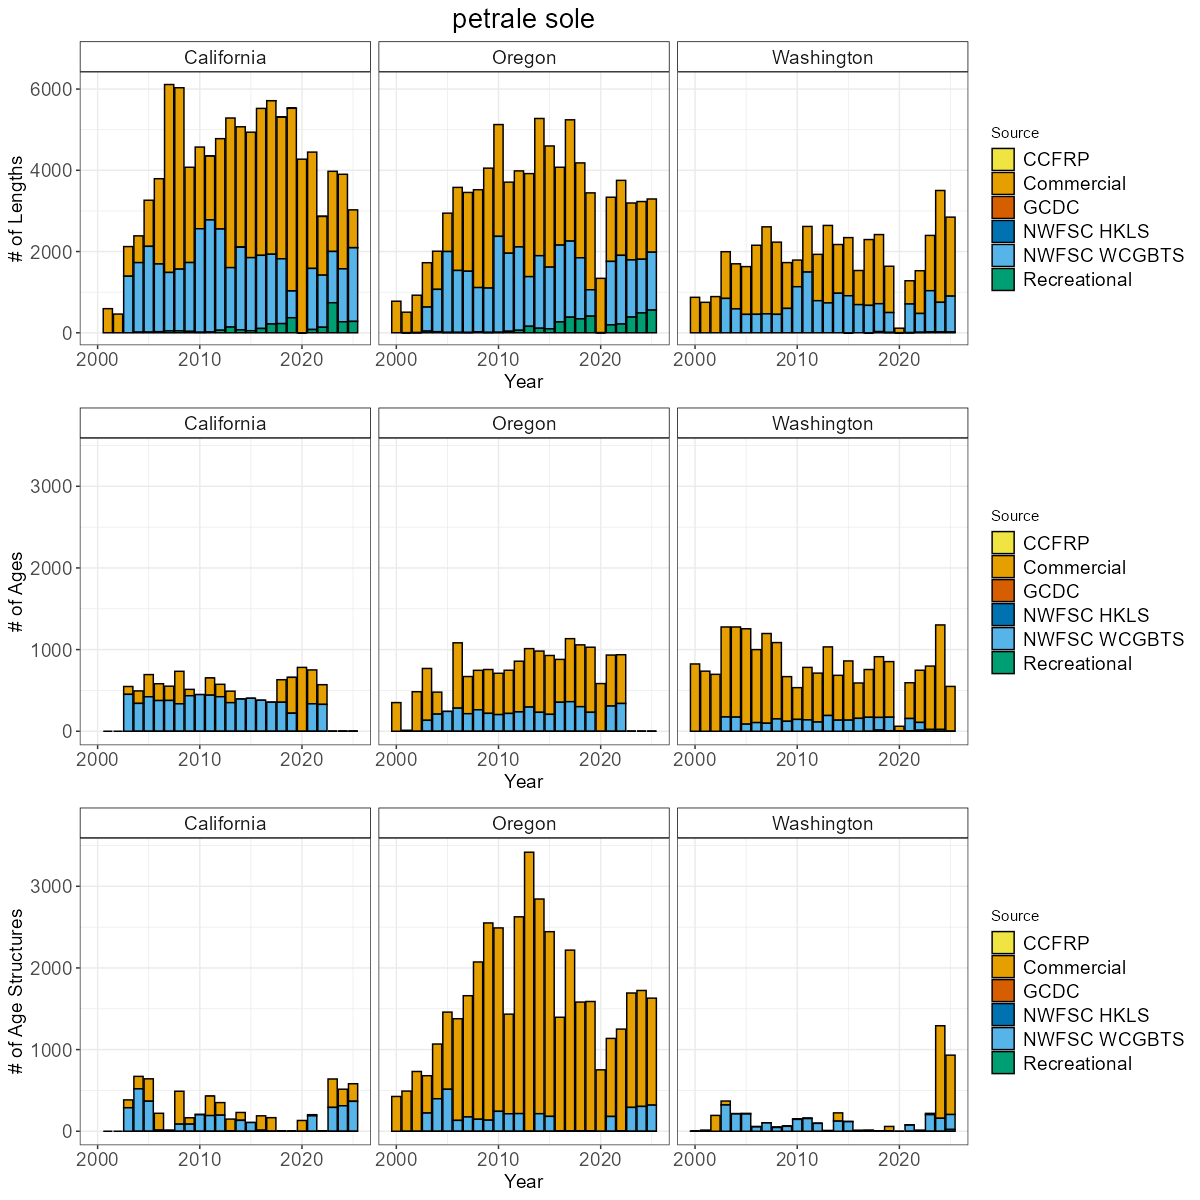
\includegraphics[width=0.95\linewidth,height=\textheight,keepaspectratio]{../plots/state_comparisons/petrale_sole_state_compositions.png}

}

\caption{Total number of available lengths, read ages, and unread age
structures by data source by year for petrale sole. Note the y-axis
maximum may differ by data type.}

\end{figure}%

\begin{figure}[H]

{\centering 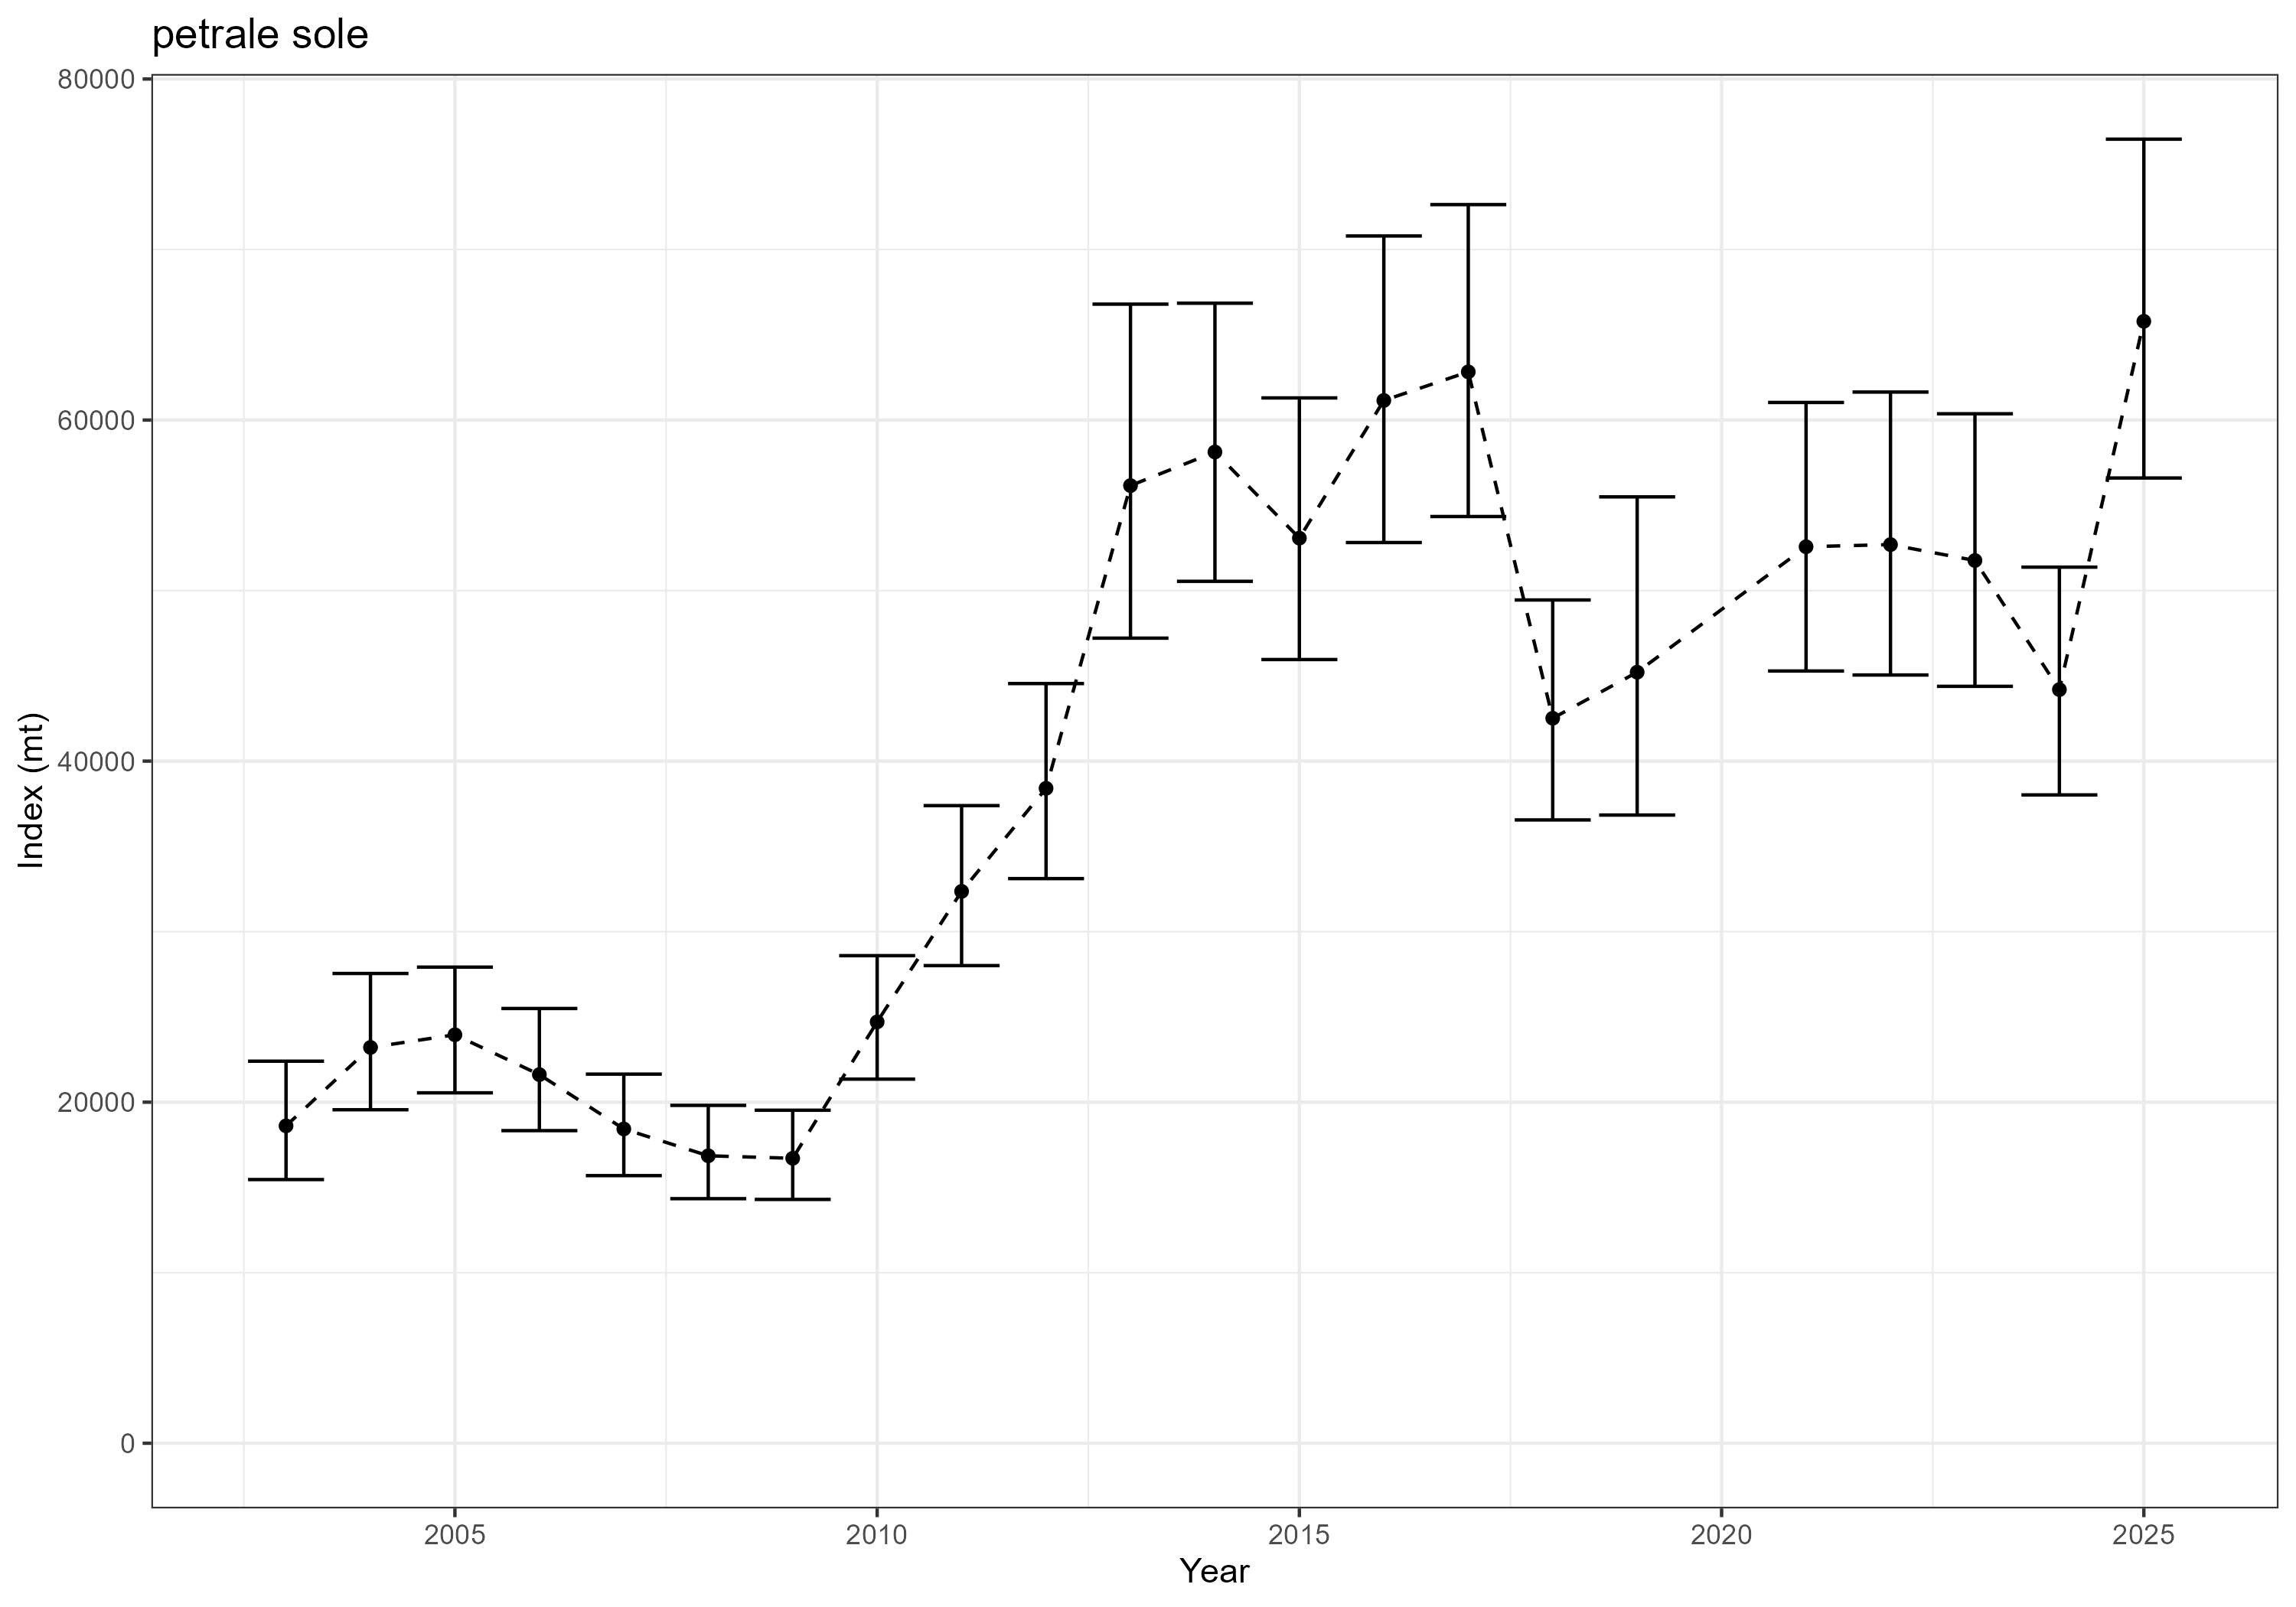
\includegraphics[width=0.95\linewidth,height=\textheight,keepaspectratio]{../plots/wcgbts_indices/petrale_sole_index.png}

}

\caption{Estimated relative index of abundance for petrale sole from the
NWFSC WCGBTS.}

\end{figure}%

\begin{figure}[H]

{\centering 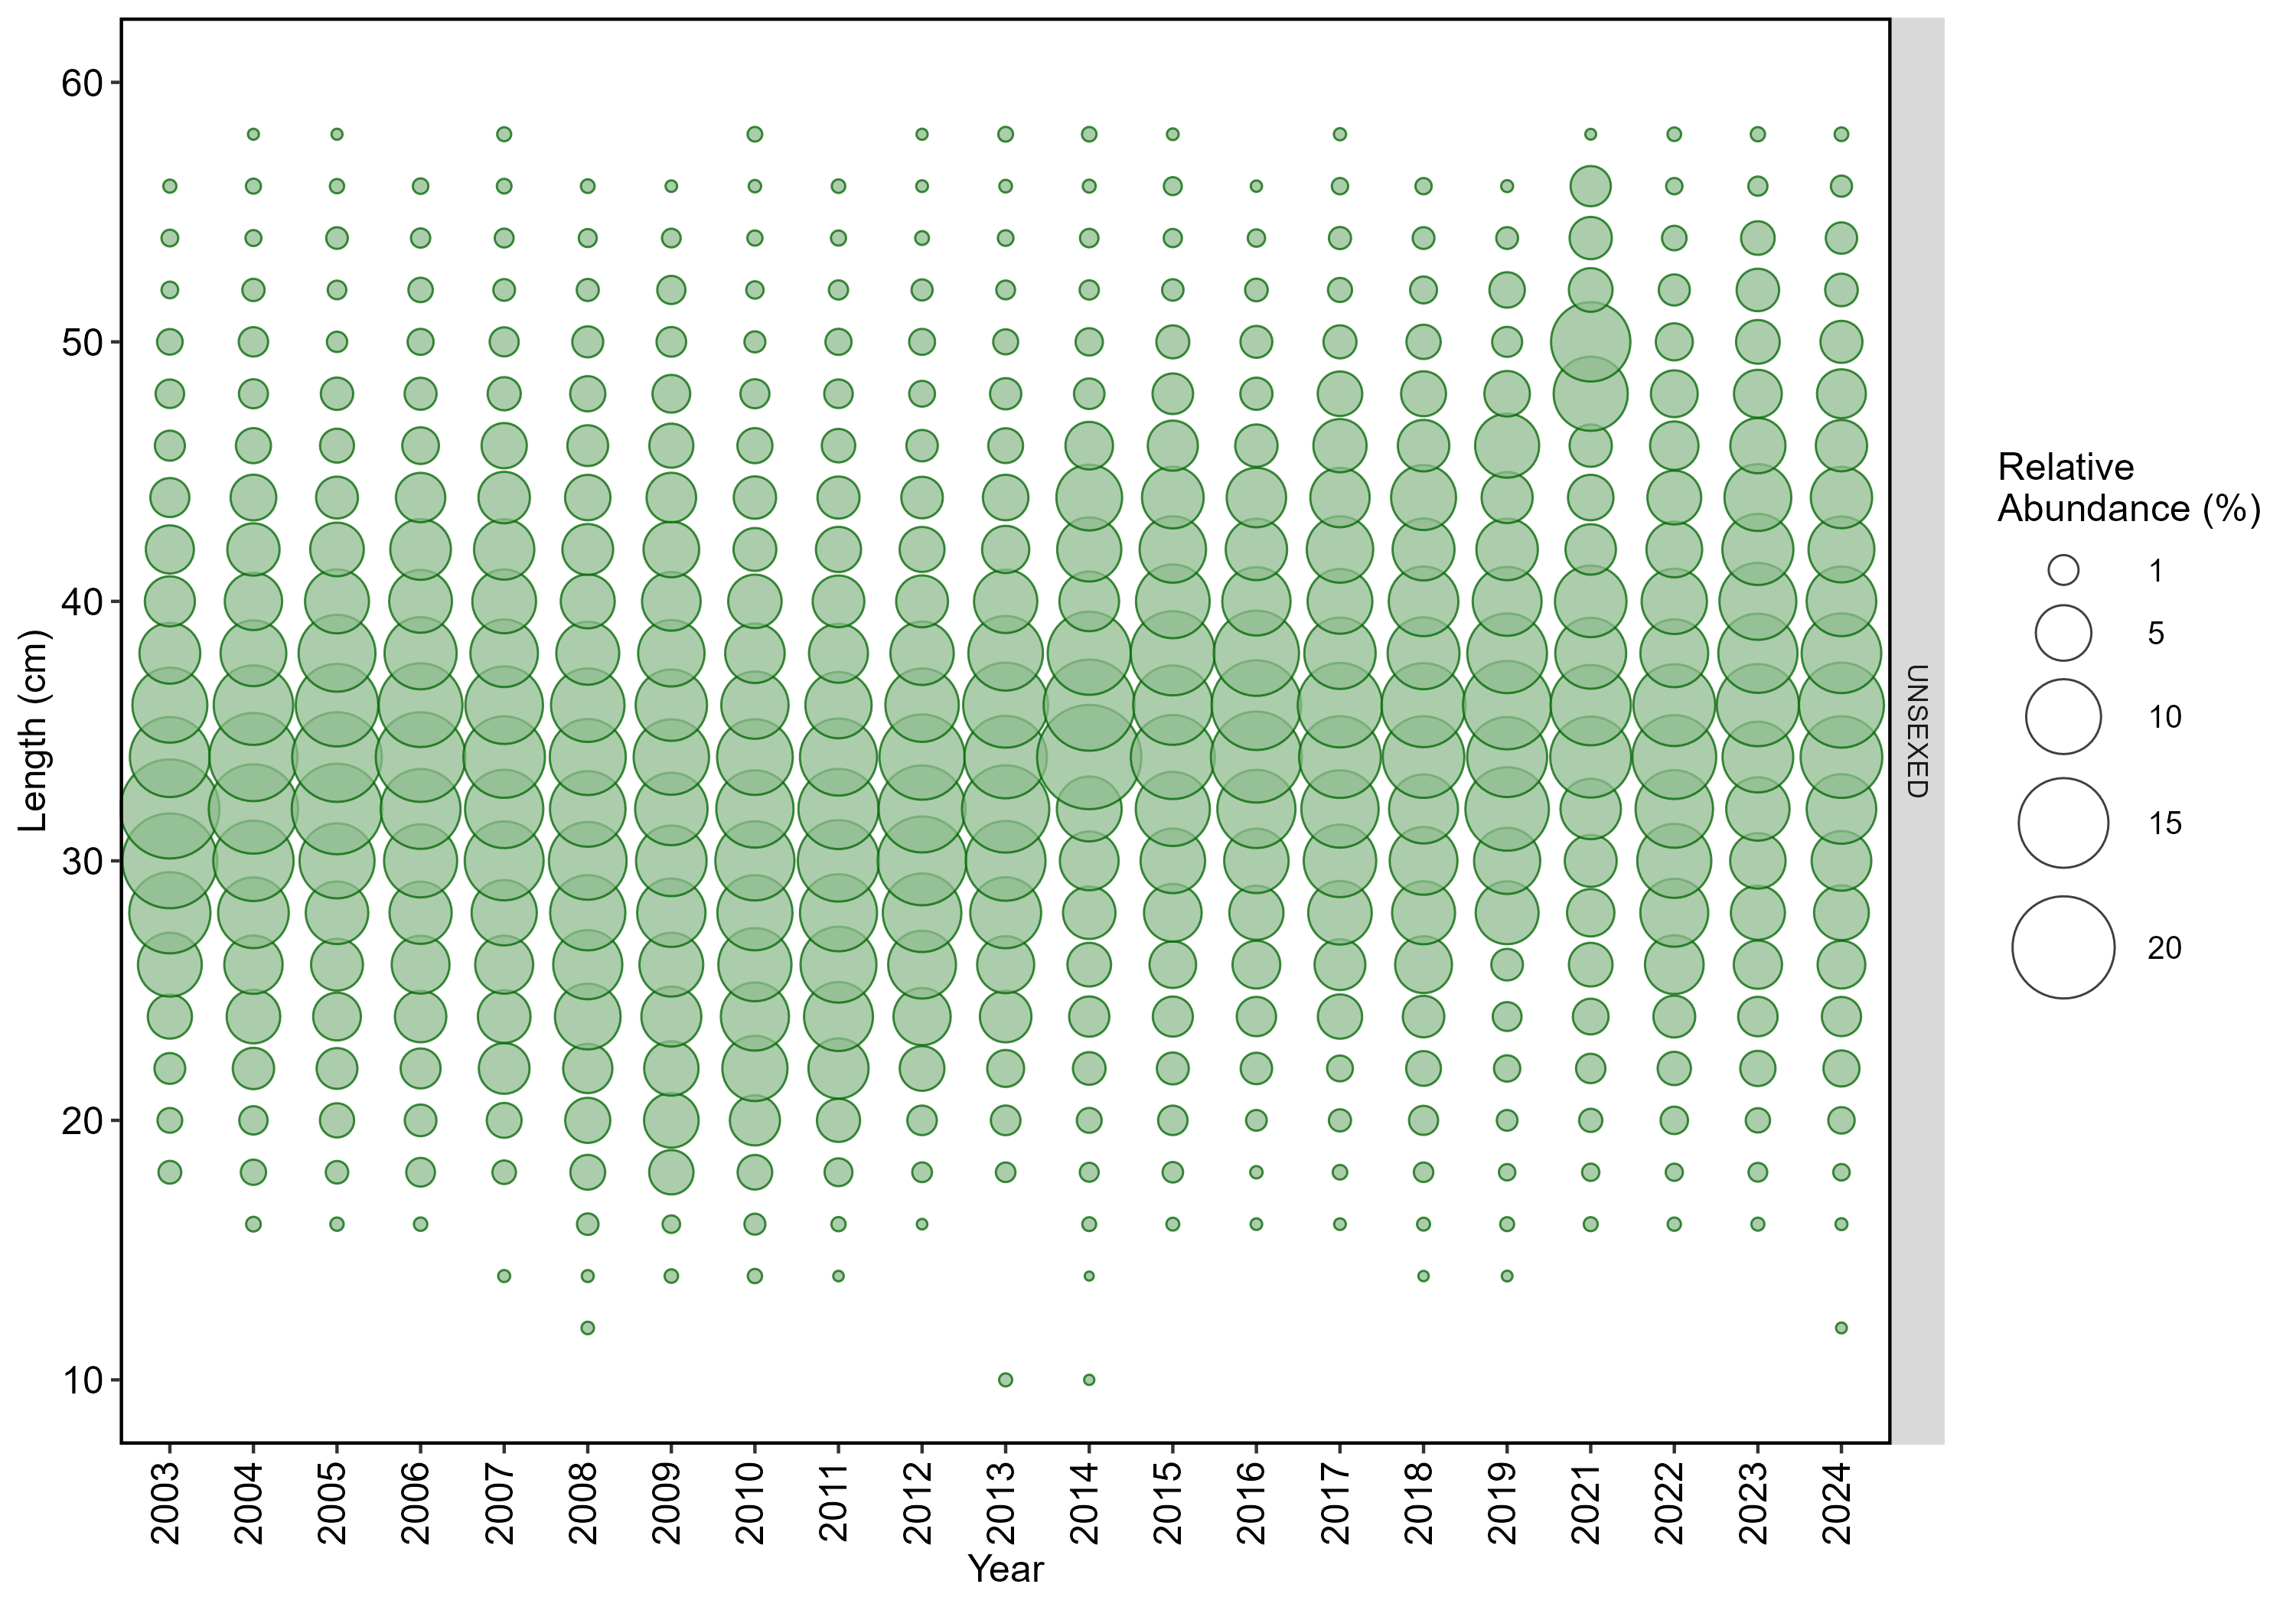
\includegraphics[width=0.95\linewidth,height=\textheight,keepaspectratio]{../plots/wcgbts_comps/plots/petrale sole_length_frequency_sex_0.png}

}

\caption{Length (cm) compostion data from the NWFSC WCGBTS for petrale
sole. Size of the circles within a year indicate higher (larger circles)
and lower (smaller circles) proportion observed by length bin.}

\end{figure}%

\newpage{}

\subsection{Quillback rockfish}\label{quillback-rockfish}

The most recent assessment of quillback rockfish was a data-moderate
assessment conducted in 2021. Across available data, quillback rockfish
have been observed and sampled by the NWFSC WCGBTS. The NWFSC WCGBTS
observed quillback rockfish on an average of 4 tows per year. For this
species, a total of 167 maturity samples have been collected coastwide
(regardless of stock area), with 162 read maturities. ODFW scientists
have conducted research looking at the influences of hypoxia on the
catch per unit effort for quillback rockfish.

\begingroup\fontsize{10}{12}\selectfont
\begingroup\fontsize{10}{12}\selectfont

\begin{longtable}[t]{>{\raggedleft\arraybackslash}p{2cm}>{\raggedleft\arraybackslash}p{3.5cm}>{\raggedleft\arraybackslash}p{2cm}>{\raggedleft\arraybackslash}p{2cm}>{\raggedleft\arraybackslash}p{2cm}}
\caption{\label{tab:unnamed-chunk-448}Total number of available lengths, read ages, and unread age structures by data source and
state for quillback rockfish.}\\
\toprule
State & Source & Lengths & Ages & Age Structures\\
\midrule
\endfirsthead
\caption[]{Total number of available lengths, read ages, and unread age structures by data source and
state for quillback rockfish. (\textit{continued)}}\\
\toprule
State & Source & Lengths & Ages & Age Structures\\
\midrule
\endhead

\endfoot
\bottomrule
\endlastfoot
OR & NWFSC WCGBTS & 133 & 89 & 27\\
WA & NWFSC WCGBTS & 107 & 75 & 11\\*
\end{longtable}
\endgroup{}
\endgroup{}

\begin{figure}[H]

{\centering 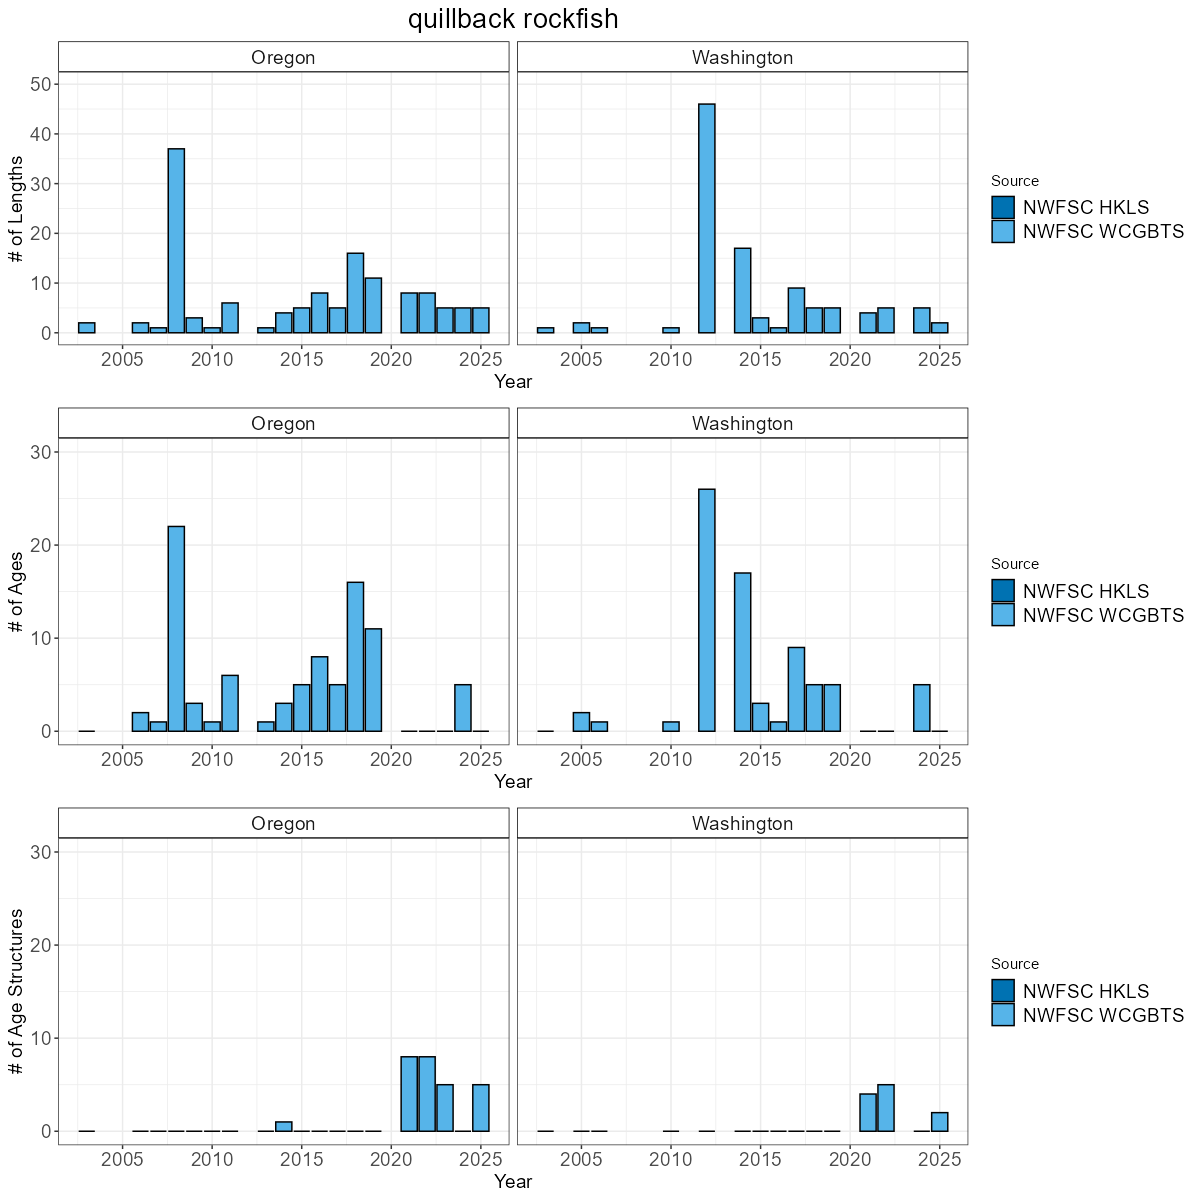
\includegraphics[width=0.95\linewidth,height=\textheight,keepaspectratio]{../plots/state_comparisons/quillback_rockfish_state_compositions.png}

}

\caption{Total number of available lengths, read ages, and unread age
structures by data source by year for quillback rockfish. Note the
y-axis maximum may differ by data type.}

\end{figure}%

\newpage{}

\subsection{Redbanded rockfish}\label{redbanded-rockfish}

To date, no assessment or analysis has been conducted on redbanded
rockfish. Across available data, redbanded rockfish have been observed
and sampled by the NWFSC WCGBTS. The NWFSC WCGBTS observed redbanded
rockfish on an average of 53 tows per year. For this species, a total of
330 maturity samples have been collected coastwide (regardless of stock
area), with 125 read maturities.

\begingroup\fontsize{10}{12}\selectfont
\begingroup\fontsize{10}{12}\selectfont

\begin{longtable}[t]{>{\raggedleft\arraybackslash}p{2cm}>{\raggedleft\arraybackslash}p{3.5cm}>{\raggedleft\arraybackslash}p{2cm}>{\raggedleft\arraybackslash}p{2cm}>{\raggedleft\arraybackslash}p{2cm}}
\caption{\label{tab:unnamed-chunk-465}Total number of available lengths, read ages, and unread age structures by data source and
state for redbanded rockfish.}\\
\toprule
State & Source & Lengths & Ages & Age Structures\\
\midrule
\endfirsthead
\caption[]{Total number of available lengths, read ages, and unread age structures by data source and
state for redbanded rockfish. (\textit{continued)}}\\
\toprule
State & Source & Lengths & Ages & Age Structures\\
\midrule
\endhead

\endfoot
\bottomrule
\endlastfoot
CA & NWFSC WCGBTS & 1,042 & 0 & 1,010\\
OR & NWFSC WCGBTS & 2,044 & 0 & 1,953\\
WA & NWFSC WCGBTS & 1,148 & 0 & 1,075\\*
\end{longtable}
\endgroup{}
\endgroup{}

\begin{figure}[H]

{\centering 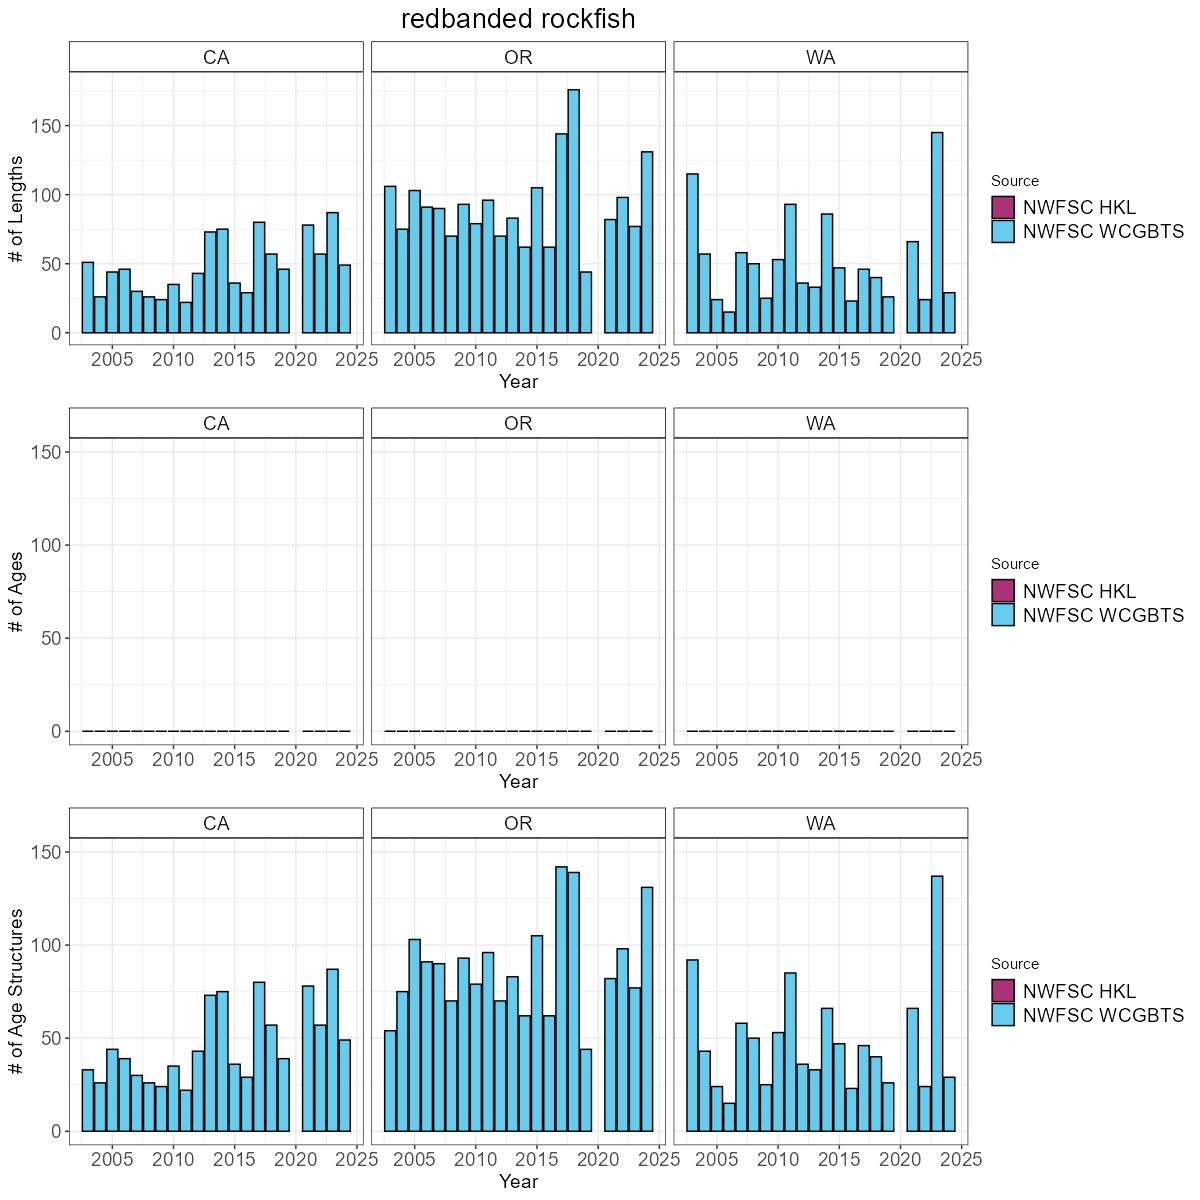
\includegraphics[width=0.95\linewidth,height=\textheight,keepaspectratio]{../plots/state_comparisons/redbanded_rockfish_state_compositions.png}

}

\caption{Total number of available lengths, read ages, and unread age
structures by data source by year for redbanded rockfish. Note the
y-axis maximum may differ by data type.}

\end{figure}%

\begin{figure}[H]

{\centering 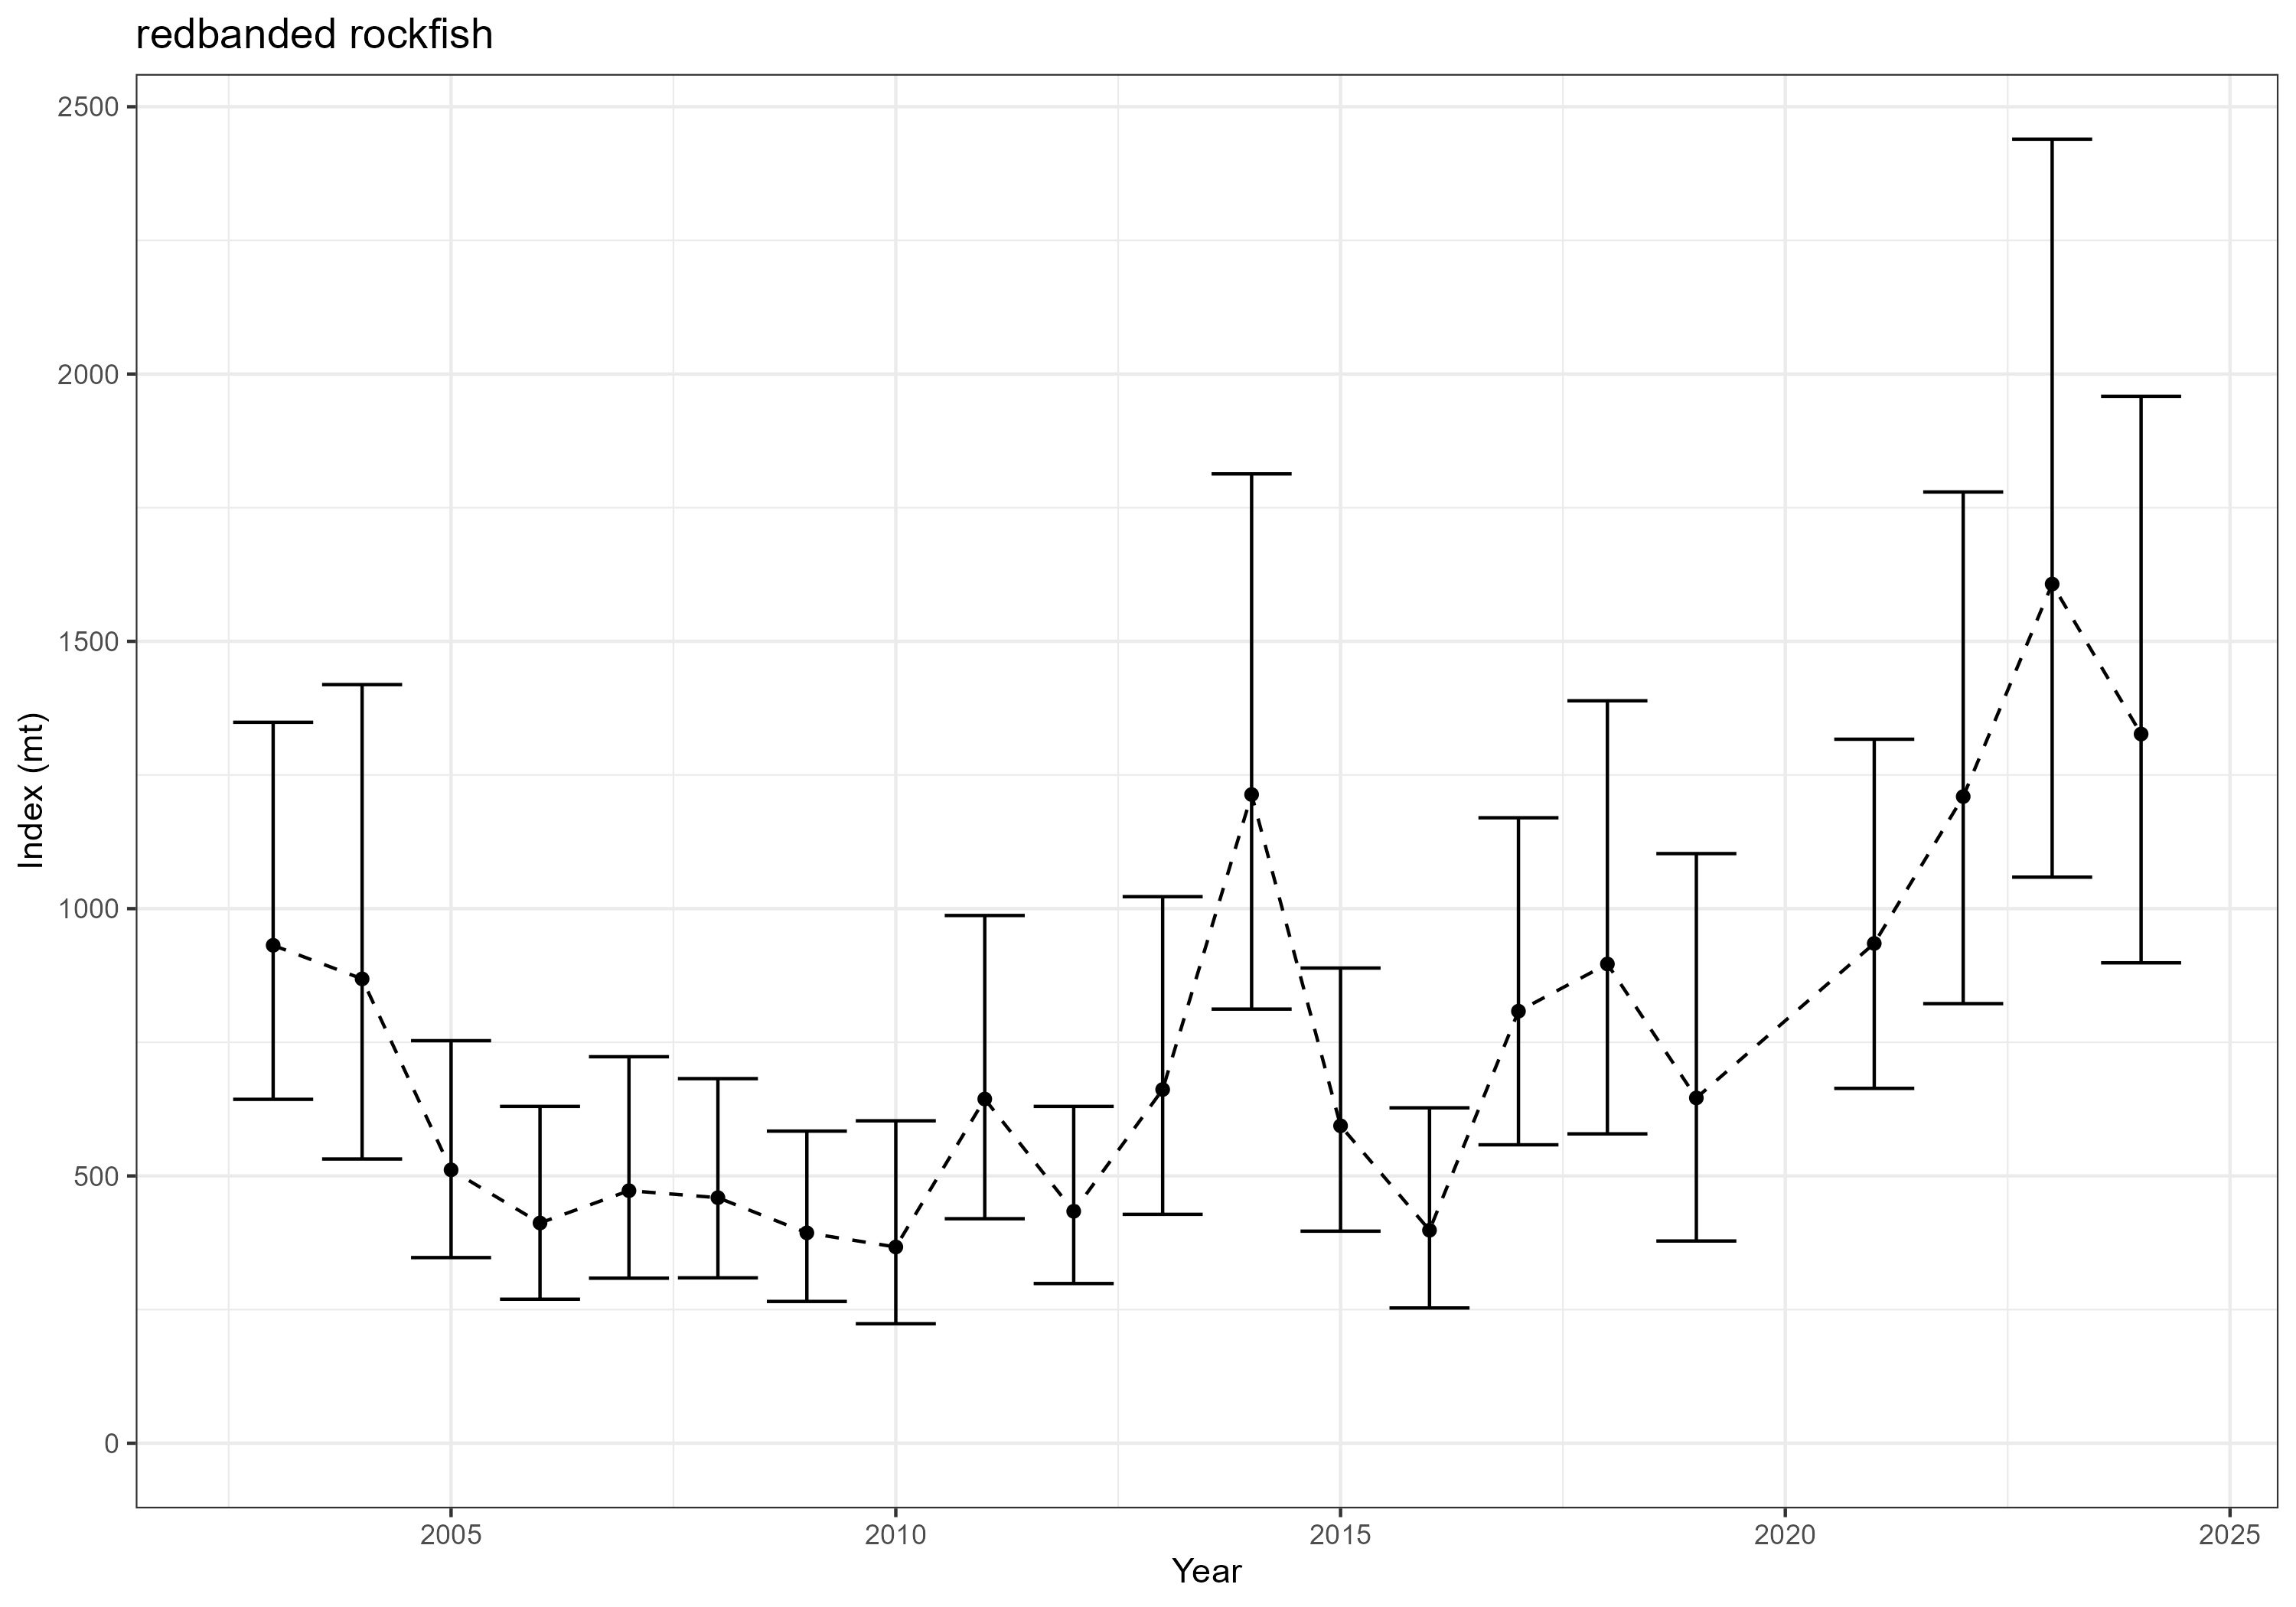
\includegraphics[width=0.95\linewidth,height=\textheight,keepaspectratio]{../plots/wcgbts_indices/redbanded_rockfish_index.png}

}

\caption{Estimated relative index of abundance for redbanded rockfish
from the NWFSC WCGBTS.}

\end{figure}%

\begin{figure}[H]

{\centering 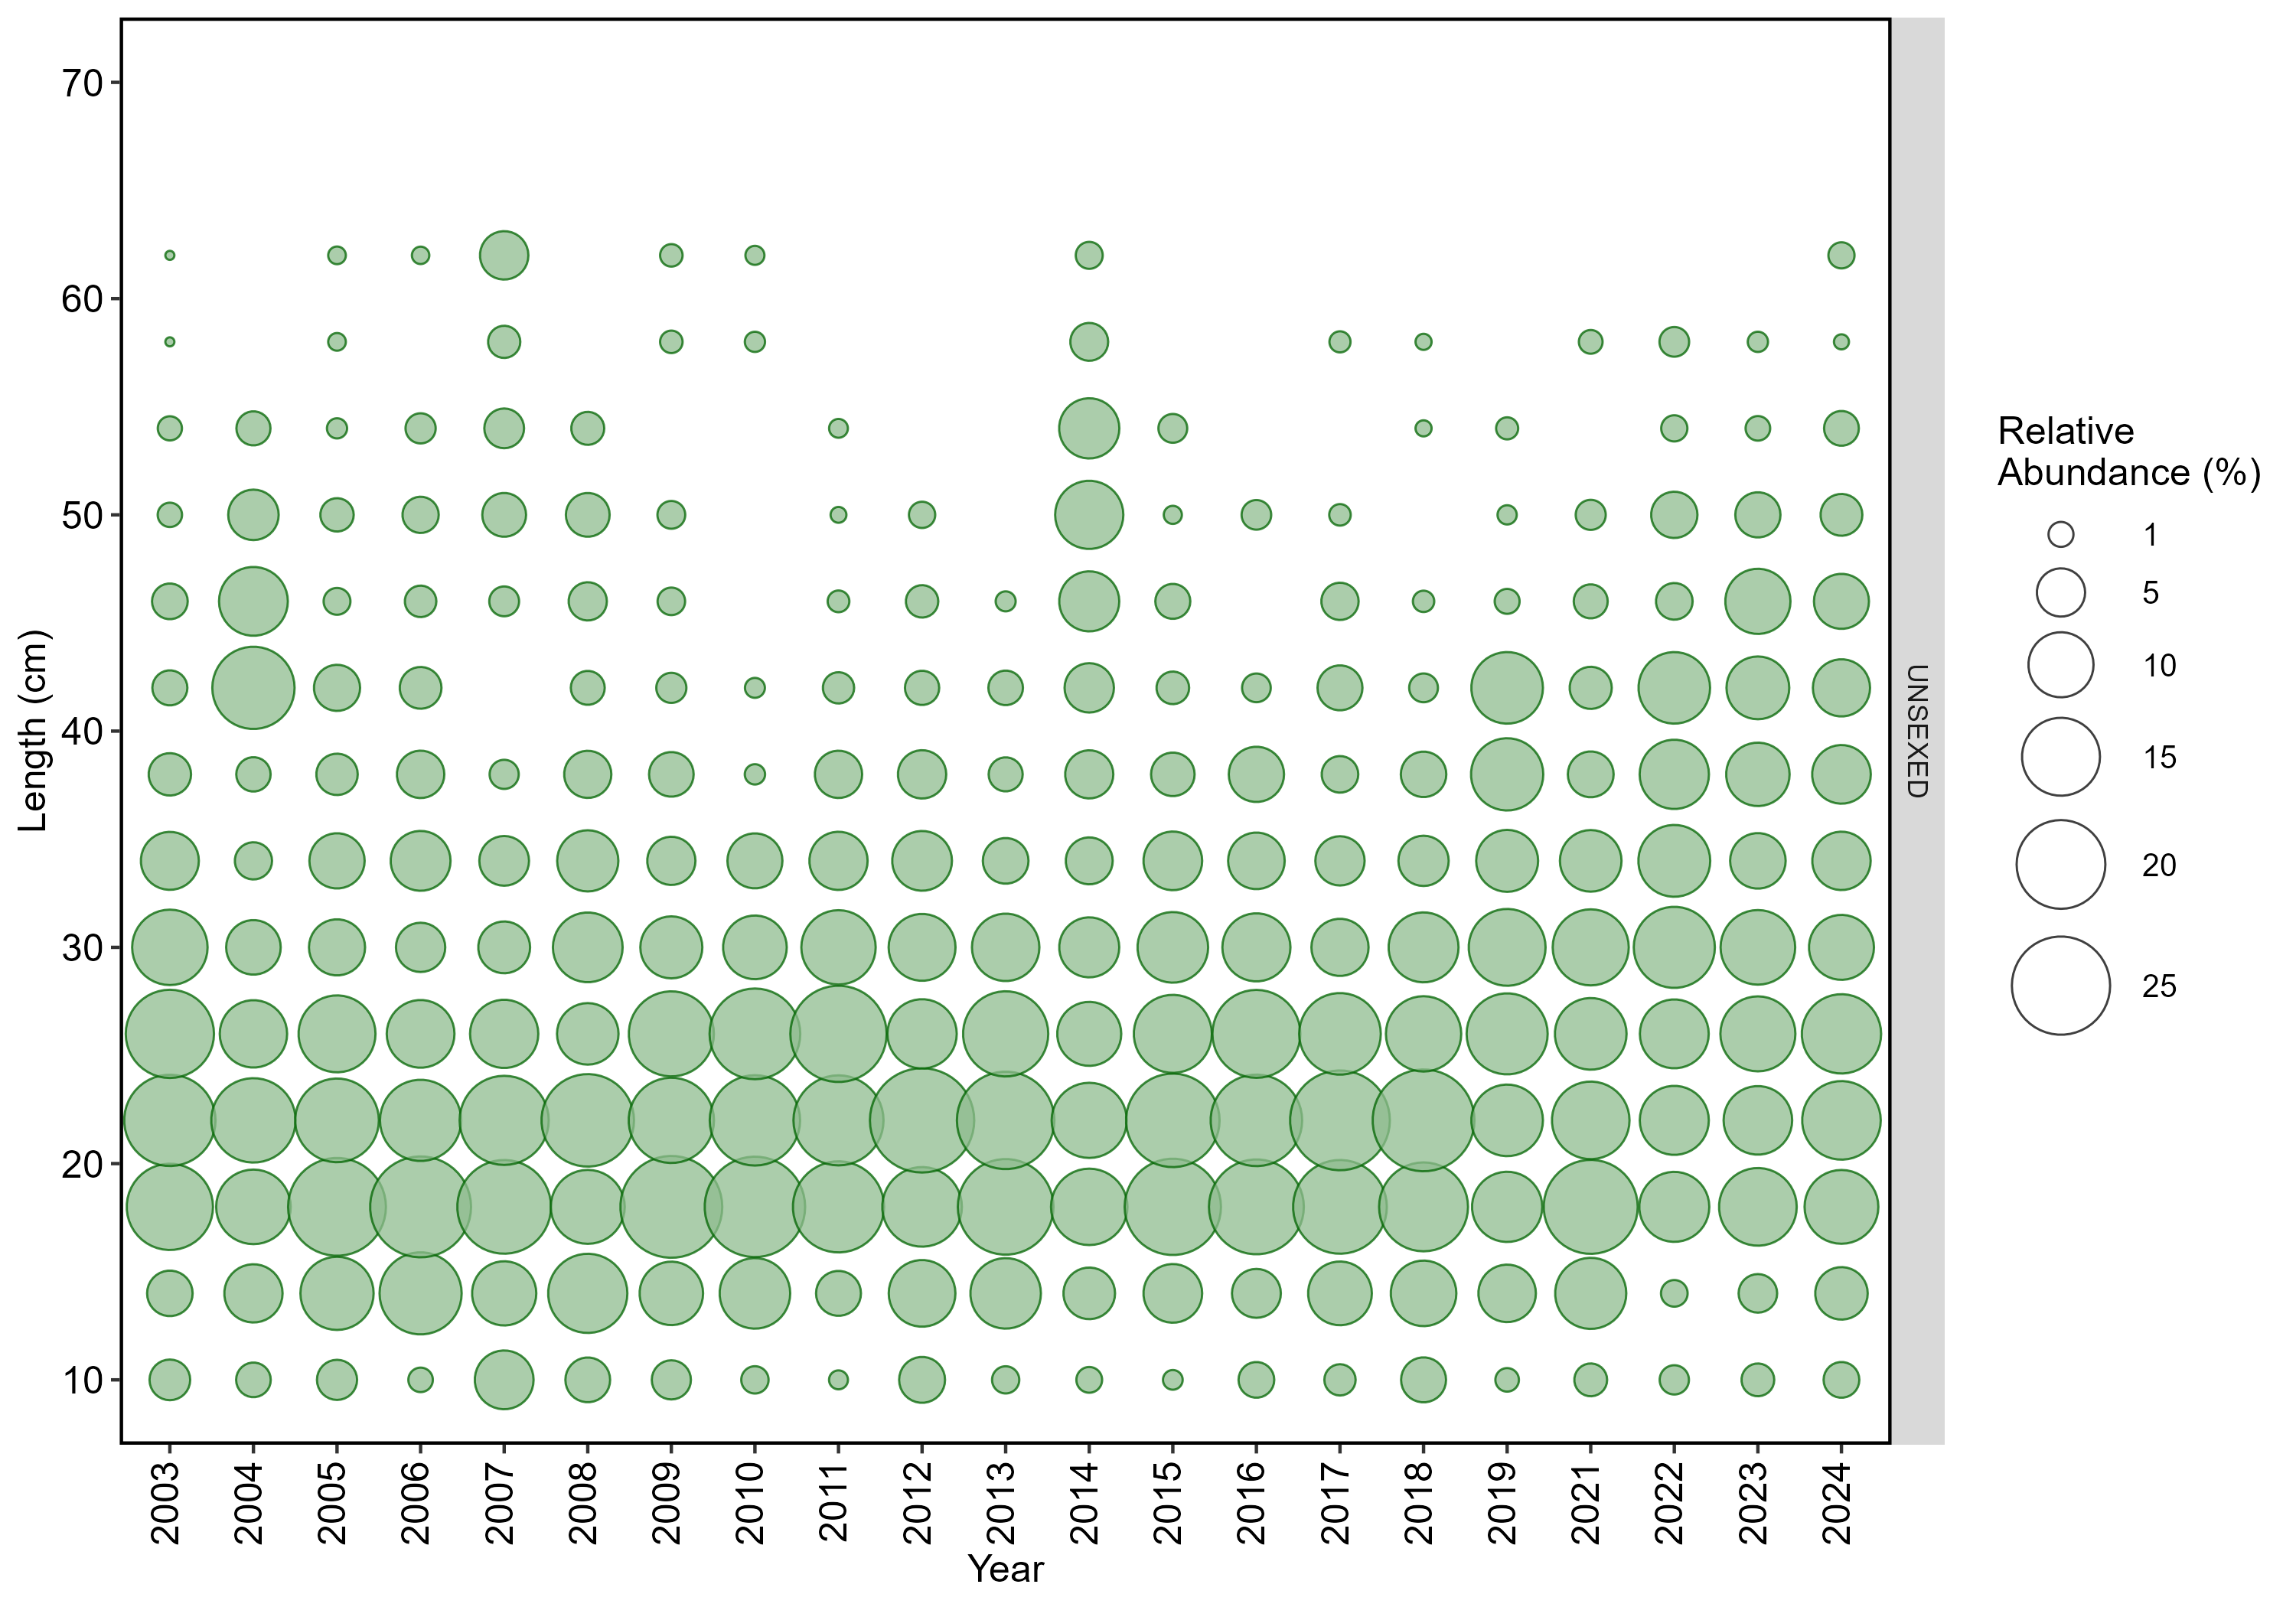
\includegraphics[width=0.95\linewidth,height=\textheight,keepaspectratio]{../plots/wcgbts_comps/plots/redbanded rockfish_length_frequency_sex_0.png}

}

\caption{Length (cm) compostion data from the NWFSC WCGBTS for redbanded
rockfish. Size of the circles within a year indicate higher (larger
circles) and lower (smaller circles) proportion observed by length bin.}

\end{figure}%

\newpage{}

\subsection{Redstripe rockfish}\label{redstripe-rockfish}

To date, no assessment or analysis has been conducted on redstripe
rockfish. Across available data, redstripe rockfish have been observed
and sampled by the NWFSC WCGBTS. The NWFSC WCGBTS observed redstripe
rockfish on an average of 12 tows per year. For this species, a total of
0 maturity samples have been collected coastwide (regardless of stock
area).

\begingroup\fontsize{10}{12}\selectfont
\begingroup\fontsize{10}{12}\selectfont

\begin{longtable}[t]{>{\raggedleft\arraybackslash}p{2cm}>{\raggedleft\arraybackslash}p{3.5cm}>{\raggedleft\arraybackslash}p{2cm}>{\raggedleft\arraybackslash}p{2cm}>{\raggedleft\arraybackslash}p{2cm}}
\caption{\label{tab:unnamed-chunk-482}Total number of available lengths, read ages, and unread age structures by data source and
state for redstripe rockfish.}\\
\toprule
State & Source & Lengths & Ages & Age Structures\\
\midrule
\endfirsthead
\caption[]{Total number of available lengths, read ages, and unread age structures by data source and
state for redstripe rockfish. (\textit{continued)}}\\
\toprule
State & Source & Lengths & Ages & Age Structures\\
\midrule
\endhead

\endfoot
\bottomrule
\endlastfoot
CA & NWFSC WCGBTS & 348 & 0 & 199\\
OR & NWFSC WCGBTS & 4,204 & 0 & 1,901\\
WA & NWFSC WCGBTS & 3,331 & 0 & 1,701\\*
\end{longtable}
\endgroup{}
\endgroup{}

\begin{figure}[H]

{\centering 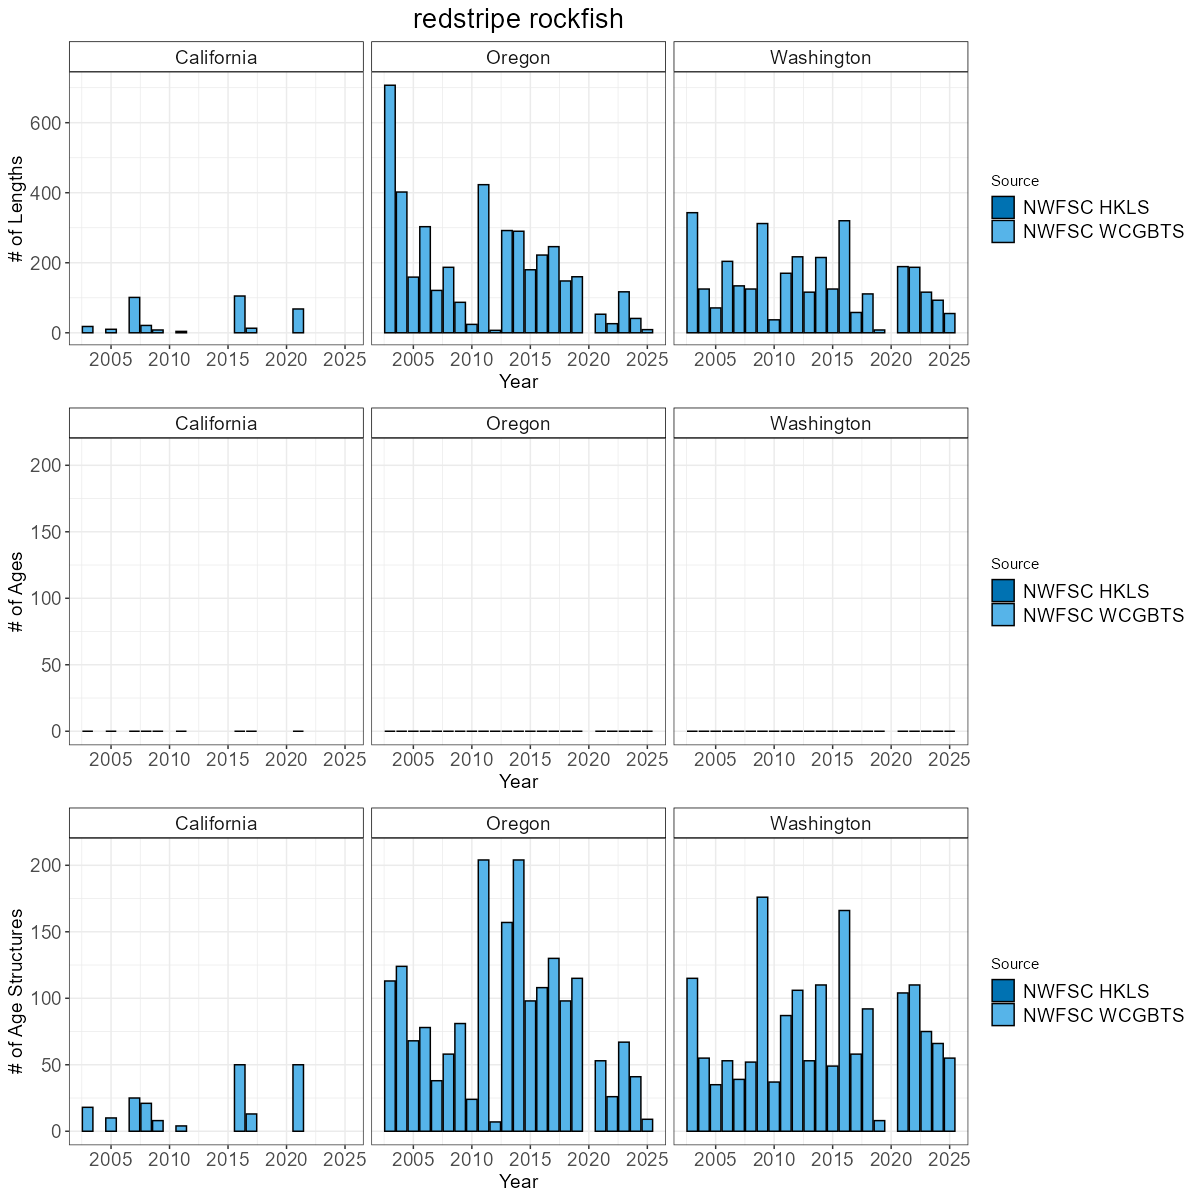
\includegraphics[width=0.95\linewidth,height=\textheight,keepaspectratio]{../plots/state_comparisons/redstripe_rockfish_state_compositions.png}

}

\caption{Total number of available lengths, read ages, and unread age
structures by data source by year for redstripe rockfish. Note the
y-axis maximum may differ by data type.}

\end{figure}%

\newpage{}

\subsection{Rex sole}\label{rex-sole}

The most recent assessment of rex sole was a data-moderate assessment
conducted in 2023. Across available data, rex sole have been observed
and sampled by the NWFSC WCGBTS. The NWFSC WCGBTS observed rex sole on
an average of 387 tows per year. For this species, a total of 0 maturity
samples have been collected coastwide (regardless of stock area).

\begingroup\fontsize{10}{12}\selectfont
\begingroup\fontsize{10}{12}\selectfont

\begin{longtable}[t]{>{\raggedleft\arraybackslash}p{2cm}>{\raggedleft\arraybackslash}p{3.5cm}>{\raggedleft\arraybackslash}p{2cm}>{\raggedleft\arraybackslash}p{2cm}>{\raggedleft\arraybackslash}p{2cm}}
\caption{\label{tab:unnamed-chunk-499}Total number of available lengths, read ages, and unread age structures by data source and
state for rex sole.}\\
\toprule
State & Source & Lengths & Ages & Age Structures\\
\midrule
\endfirsthead
\caption[]{Total number of available lengths, read ages, and unread age structures by data source and
state for rex sole. (\textit{continued)}}\\
\toprule
State & Source & Lengths & Ages & Age Structures\\
\midrule
\endhead

\endfoot
\bottomrule
\endlastfoot
CA & NWFSC WCGBTS & 59,213 & 273 & 5,082\\
OR & NWFSC WCGBTS & 69,896 & 208 & 4,874\\
WA & NWFSC WCGBTS & 25,890 & 140 & 1,992\\*
\end{longtable}
\endgroup{}
\endgroup{}

\begin{figure}[H]

{\centering 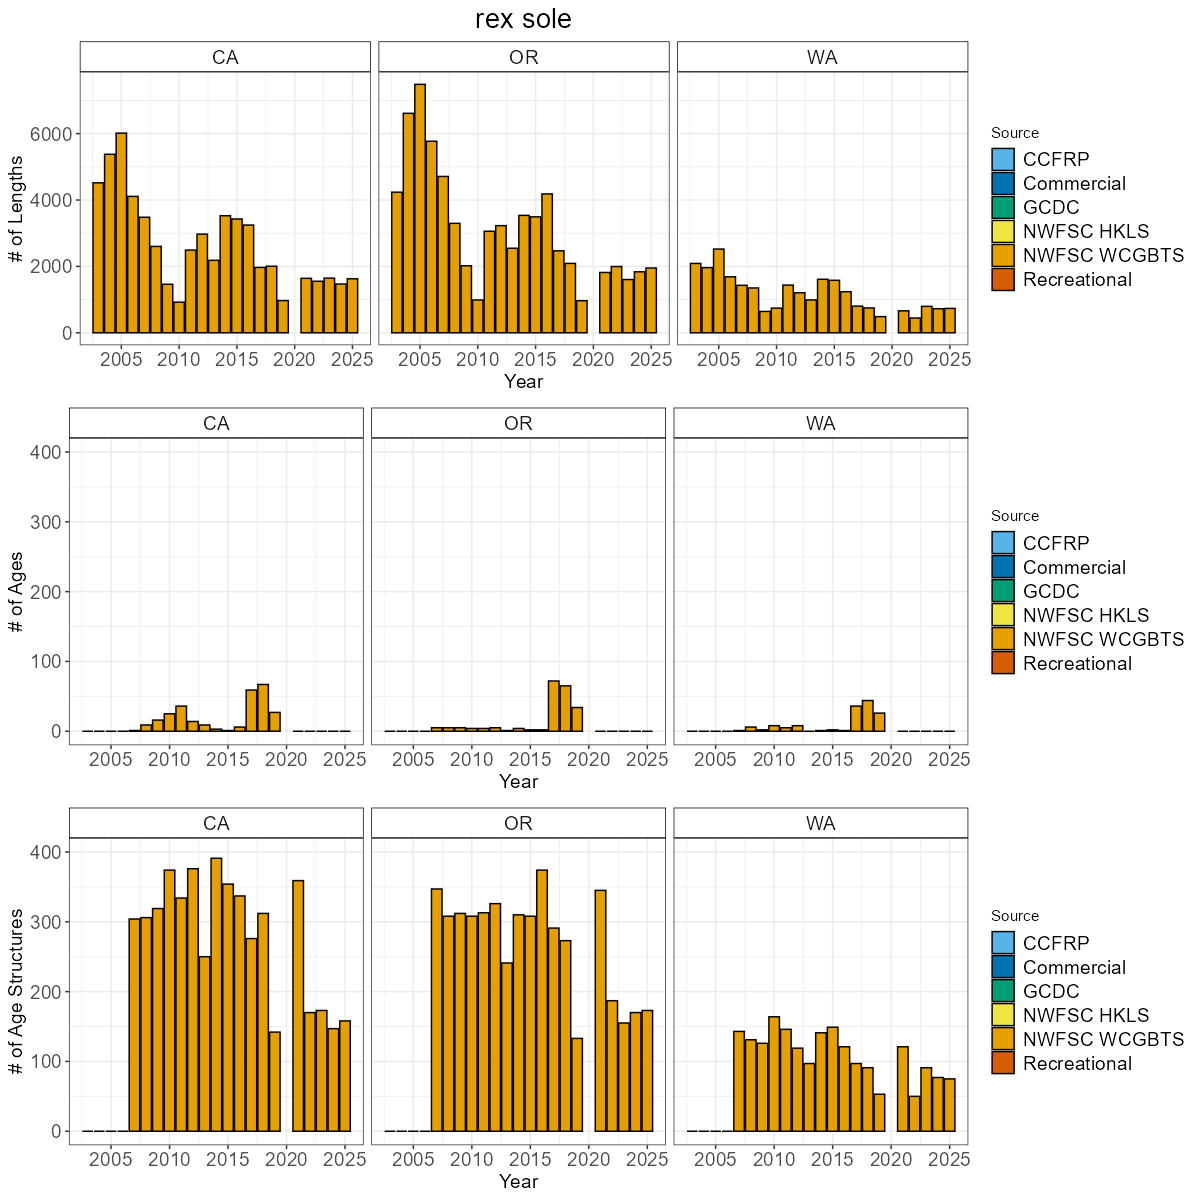
\includegraphics[width=0.95\linewidth,height=\textheight,keepaspectratio]{../plots/state_comparisons/rex_sole_state_compositions.png}

}

\caption{Total number of available lengths, read ages, and unread age
structures by data source by year for rex sole. Note the y-axis maximum
may differ by data type.}

\end{figure}%

\begin{figure}[H]

{\centering 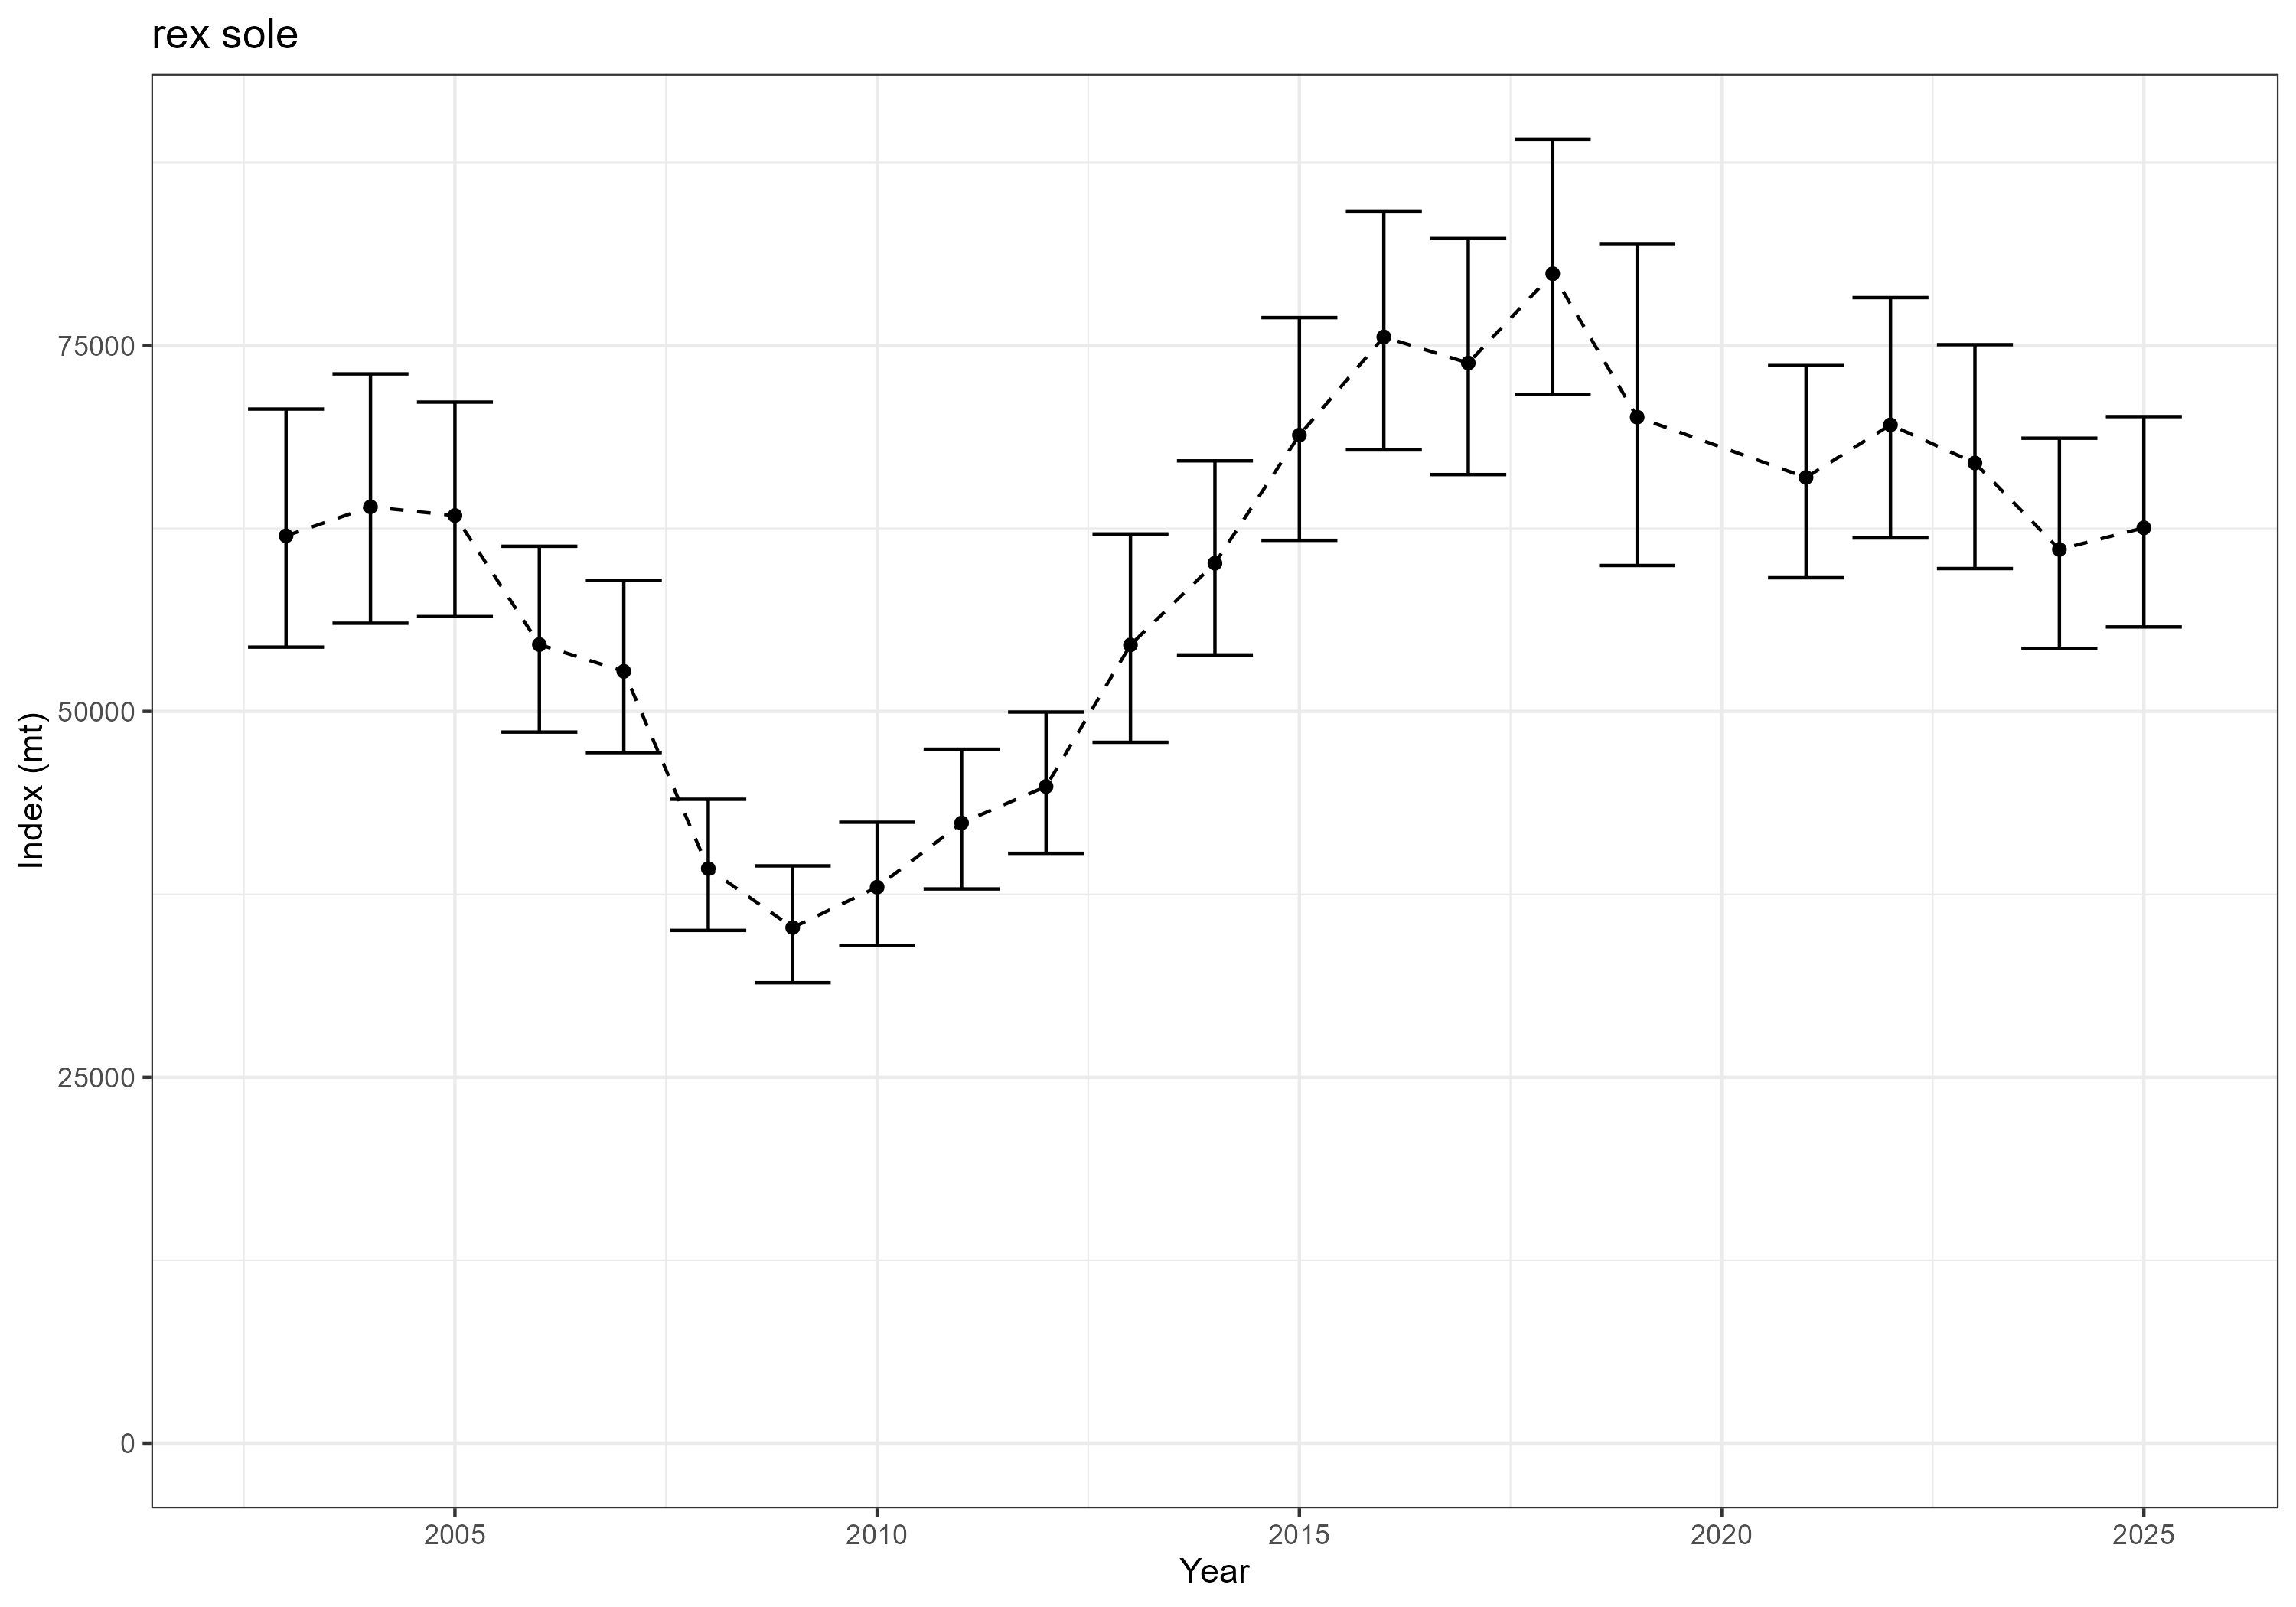
\includegraphics[width=0.95\linewidth,height=\textheight,keepaspectratio]{../plots/wcgbts_indices/rex_sole_index.png}

}

\caption{Estimated relative index of abundance for rex sole from the
NWFSC WCGBTS.}

\end{figure}%

\begin{figure}[H]

{\centering 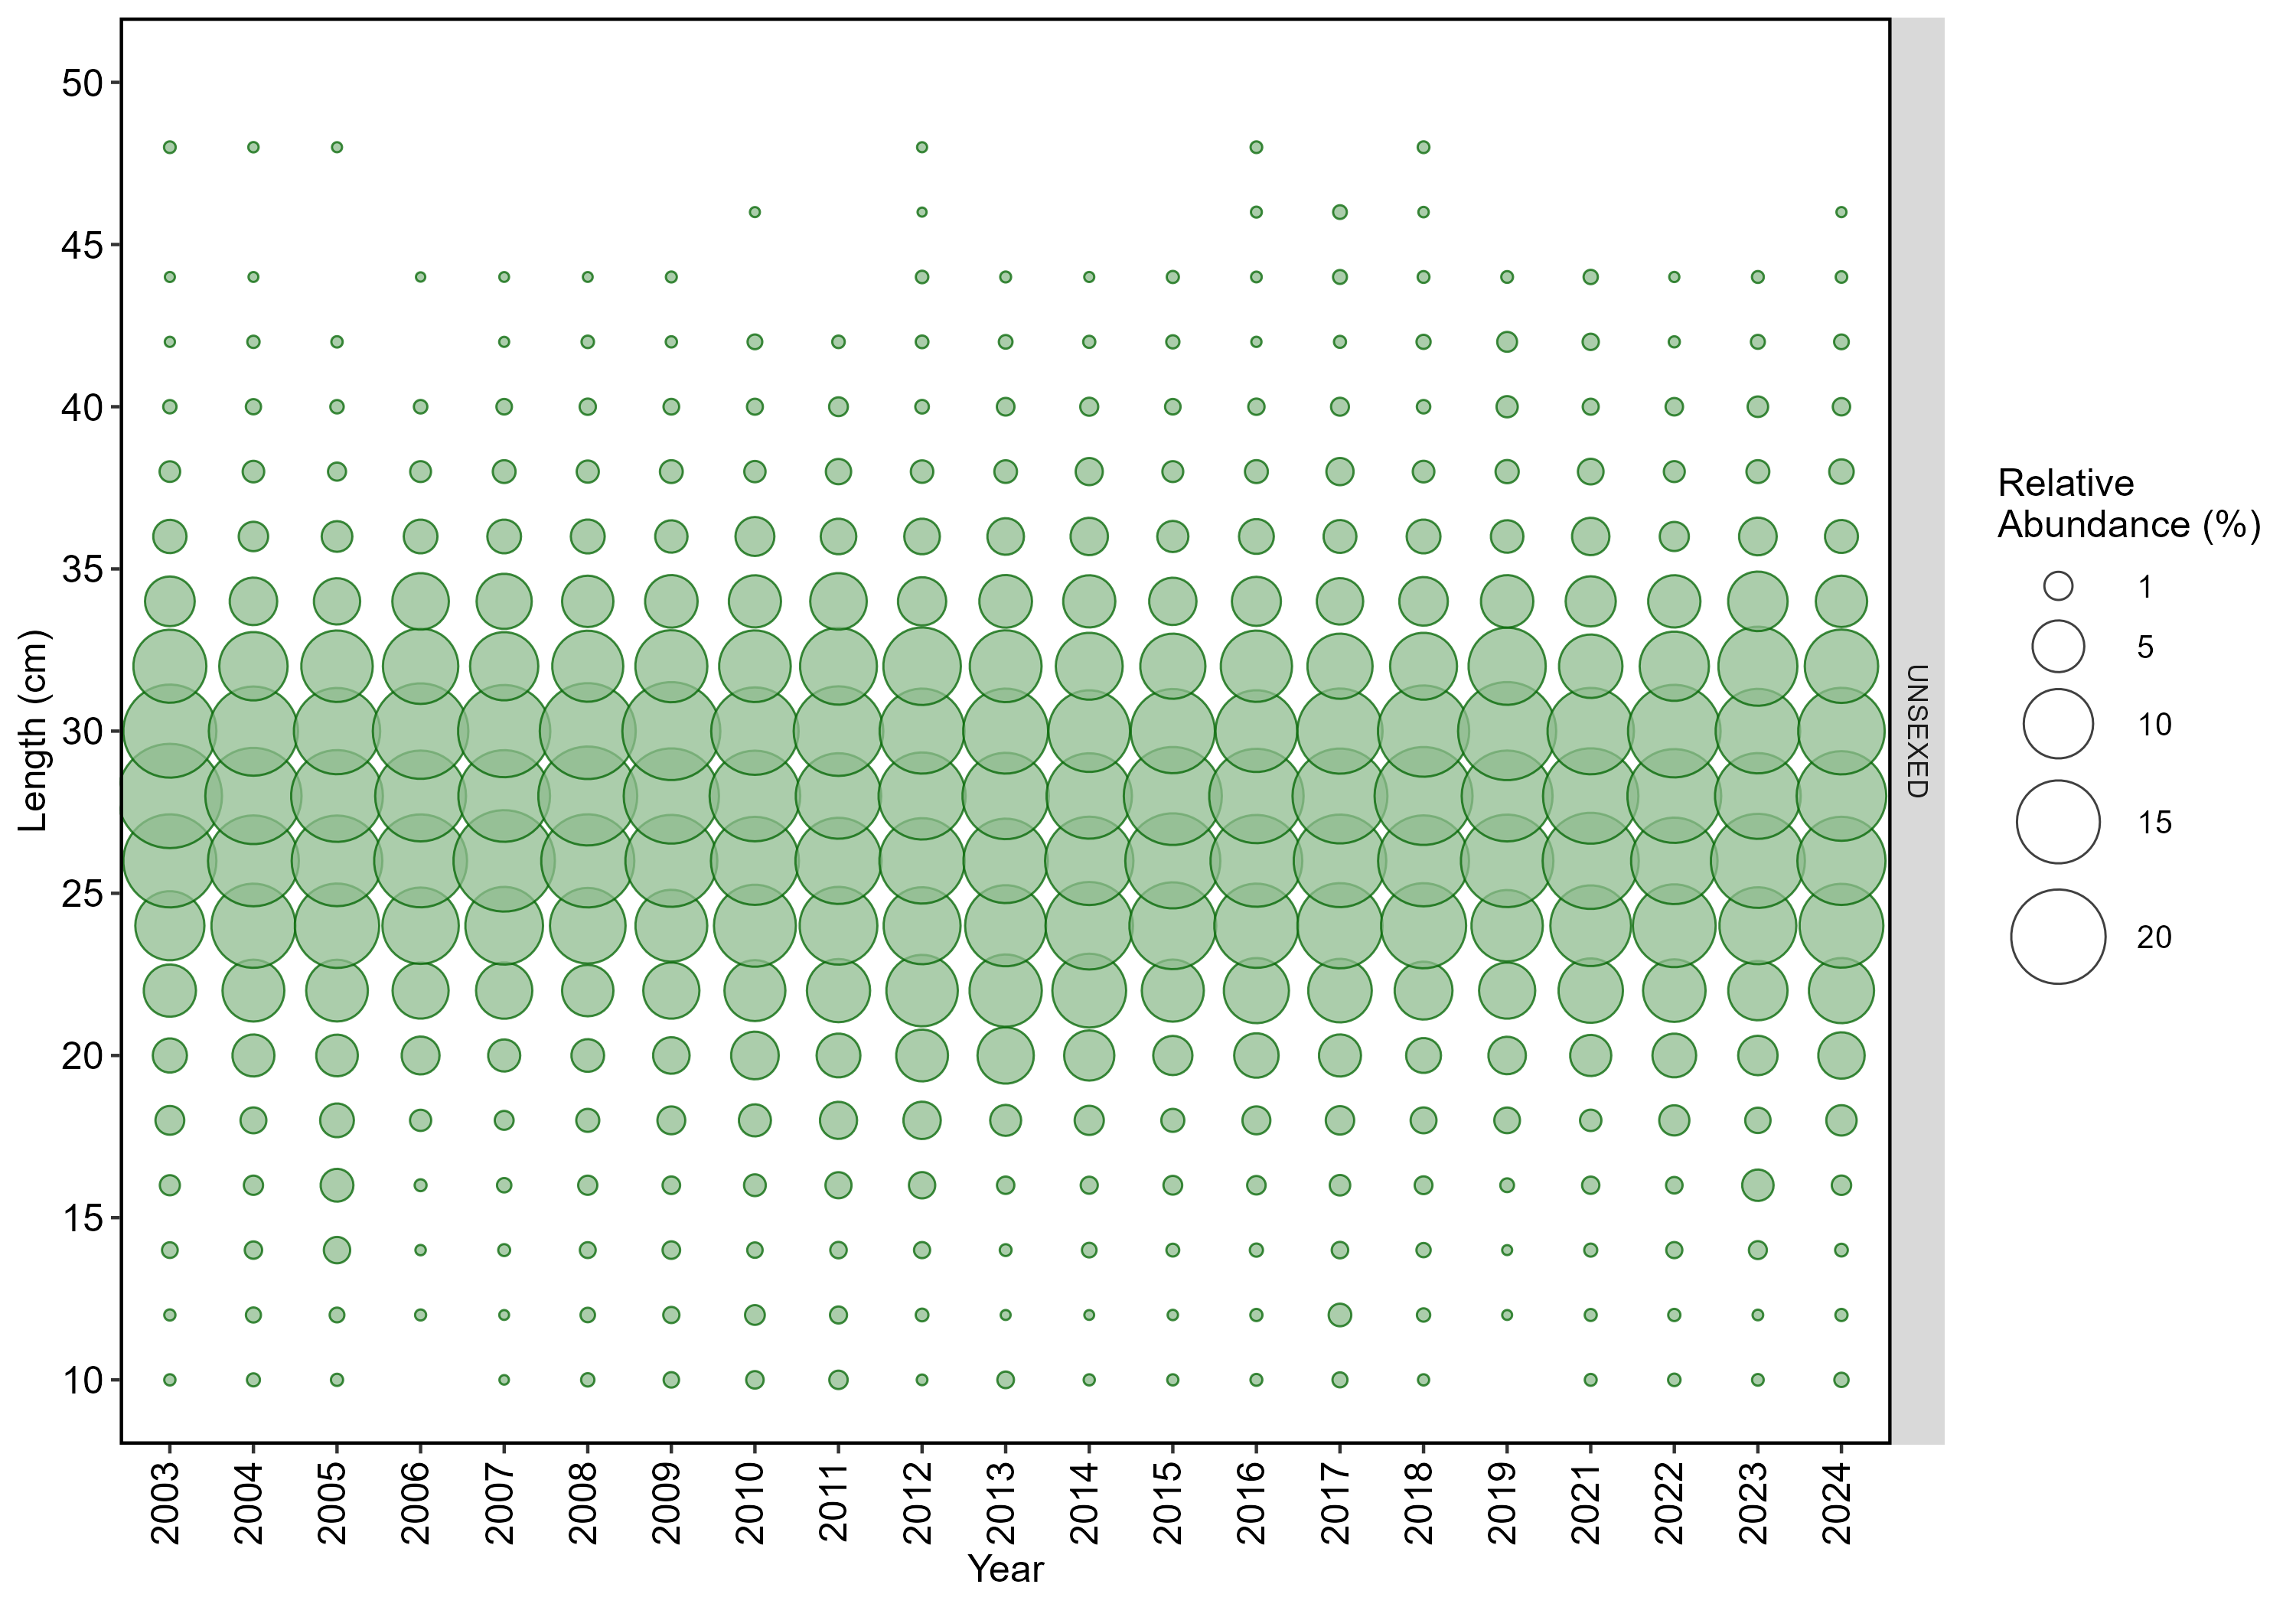
\includegraphics[width=0.95\linewidth,height=\textheight,keepaspectratio]{../plots/wcgbts_comps/plots/rex sole_length_frequency_sex_0.png}

}

\caption{Length (cm) compostion data from the NWFSC WCGBTS for rex sole.
Size of the circles within a year indicate higher (larger circles) and
lower (smaller circles) proportion observed by length bin.}

\end{figure}%

\newpage{}

\subsection{Rosethorn rockfish}\label{rosethorn-rockfish}

To date, no assessment or analysis has been conducted on rosethorn
rockfish. Across available data, rosethorn rockfish have been observed
and sampled by both the NWFSC HKLS and WCGBTS. The NWFSC HKLS observed
rosethorn rockfish at an average of 0 sets per year. The NWFSC WCGBTS
observed rosethorn rockfish on an average of 48 tows per year. For this
species, a total of 0 maturity samples have been collected coastwide
(regardless of stock area).

\begingroup\fontsize{10}{12}\selectfont
\begingroup\fontsize{10}{12}\selectfont

\begin{longtable}[t]{>{\raggedleft\arraybackslash}p{2cm}>{\raggedleft\arraybackslash}p{3.5cm}>{\raggedleft\arraybackslash}p{2cm}>{\raggedleft\arraybackslash}p{2cm}>{\raggedleft\arraybackslash}p{2cm}}
\caption{\label{tab:unnamed-chunk-516}Total number of available lengths, read ages, and unread age structures by data source and
state for rosethorn rockfish.}\\
\toprule
State & Source & Lengths & Ages & Age Structures\\
\midrule
\endfirsthead
\caption[]{Total number of available lengths, read ages, and unread age structures by data source and
state for rosethorn rockfish. (\textit{continued)}}\\
\toprule
State & Source & Lengths & Ages & Age Structures\\
\midrule
\endhead

\endfoot
\bottomrule
\endlastfoot
CA & NWFSC HKLS & 36 & 0 & 27\\
CA & NWFSC WCGBTS & 3,103 & 0 & 1,561\\
OR & NWFSC WCGBTS & 10,552 & 0 & 4,359\\
WA & NWFSC WCGBTS & 6,906 & 0 & 2,893\\*
\end{longtable}
\endgroup{}
\endgroup{}

\begin{figure}[H]

{\centering 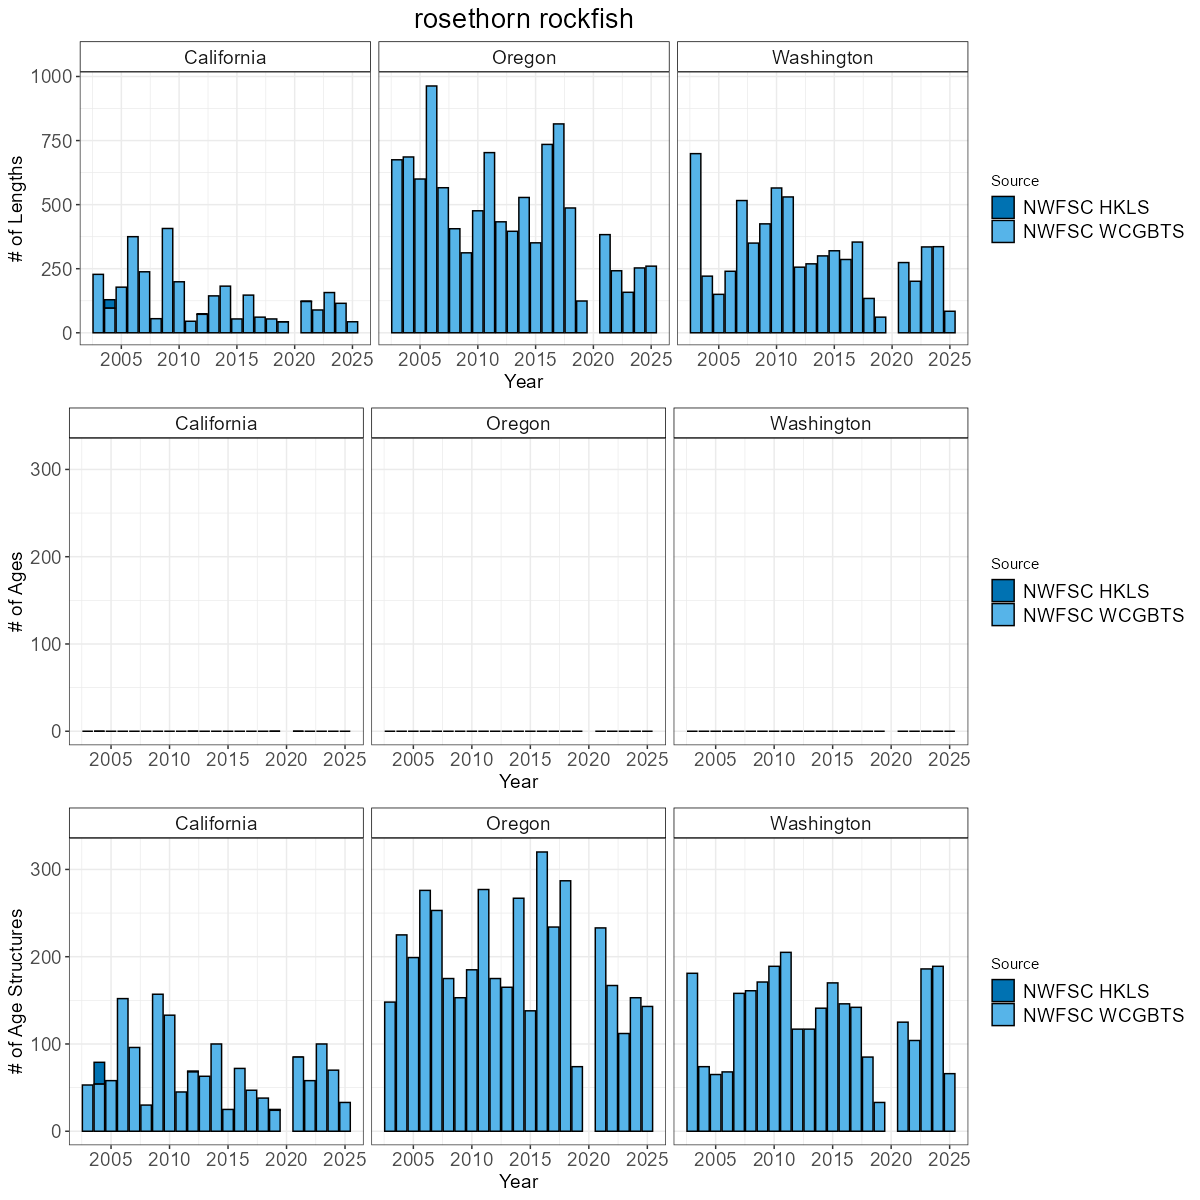
\includegraphics[width=0.95\linewidth,height=\textheight,keepaspectratio]{../plots/state_comparisons/rosethorn_rockfish_state_compositions.png}

}

\caption{Total number of available lengths, read ages, and unread age
structures by data source by year for rosethorn rockfish. Note the
y-axis maximum may differ by data type.}

\end{figure}%

\begin{figure}[H]

{\centering 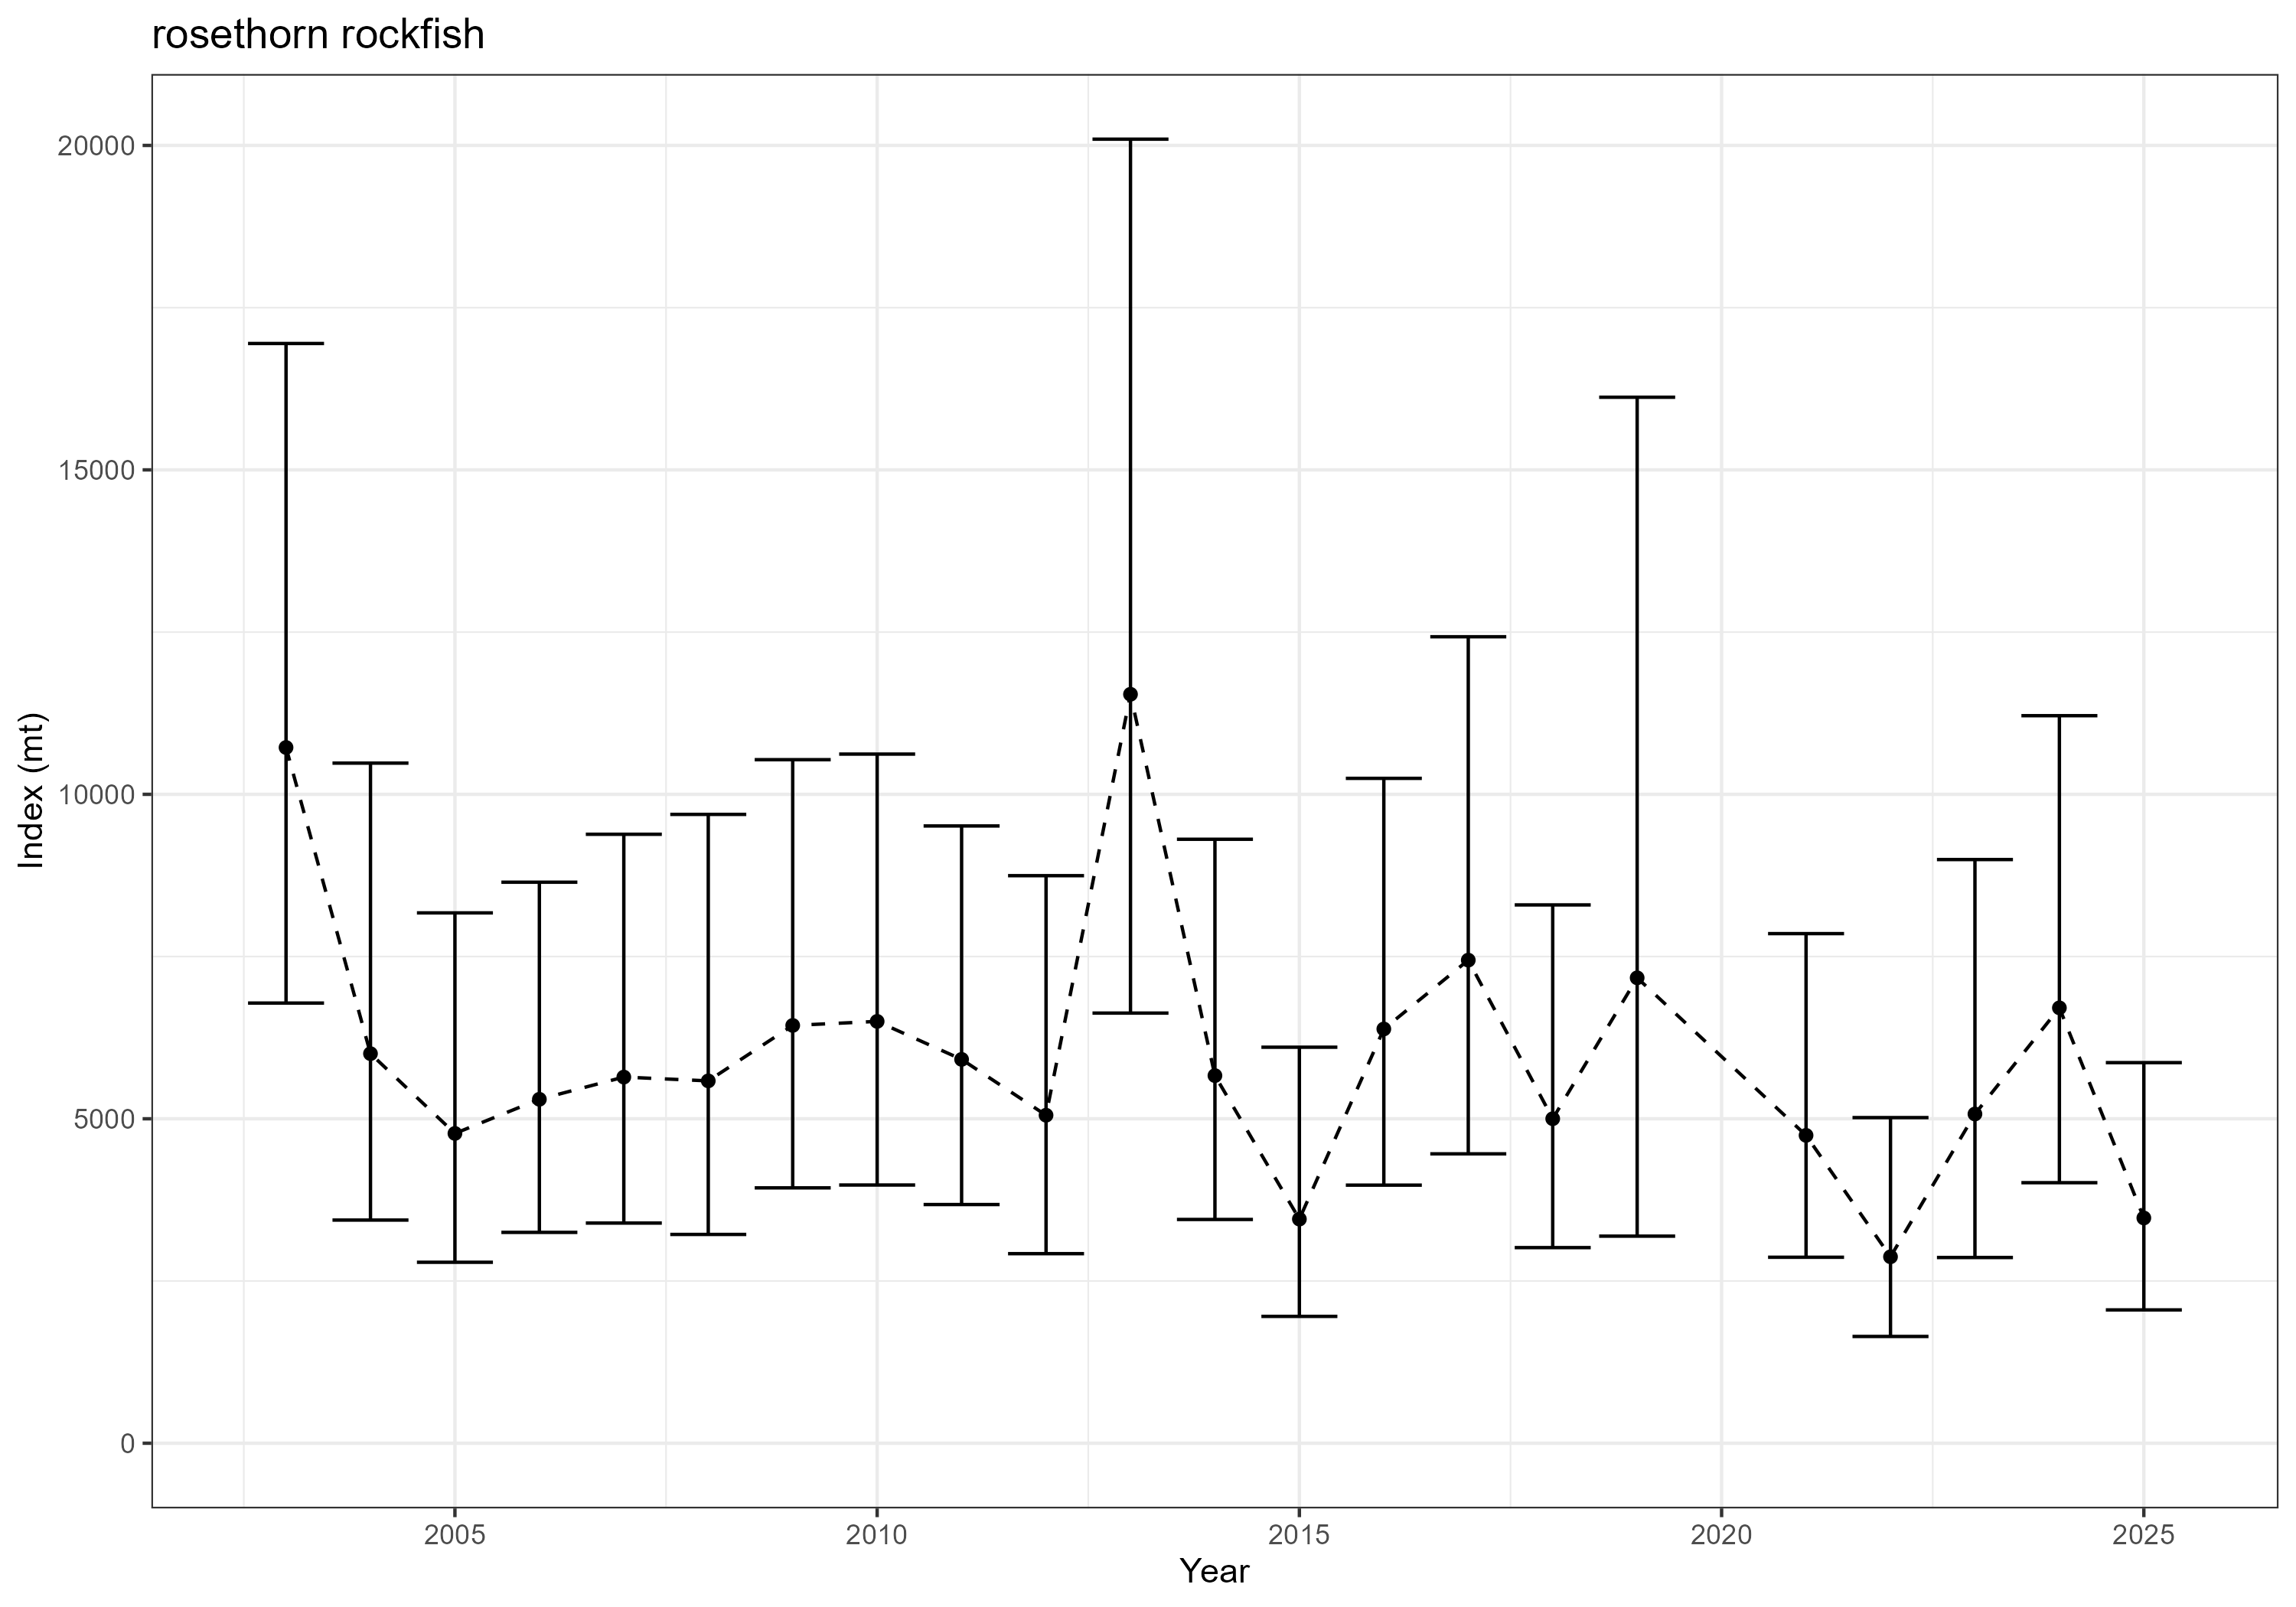
\includegraphics[width=0.95\linewidth,height=\textheight,keepaspectratio]{../plots/additional_wcgbts_indices/rosethorn_rockfish_index.png}

}

\caption{Estimated relative index of abundance for rosethorn rockfish
from the NWFSC WCGBTS.}

\end{figure}%

\begin{figure}[H]

{\centering 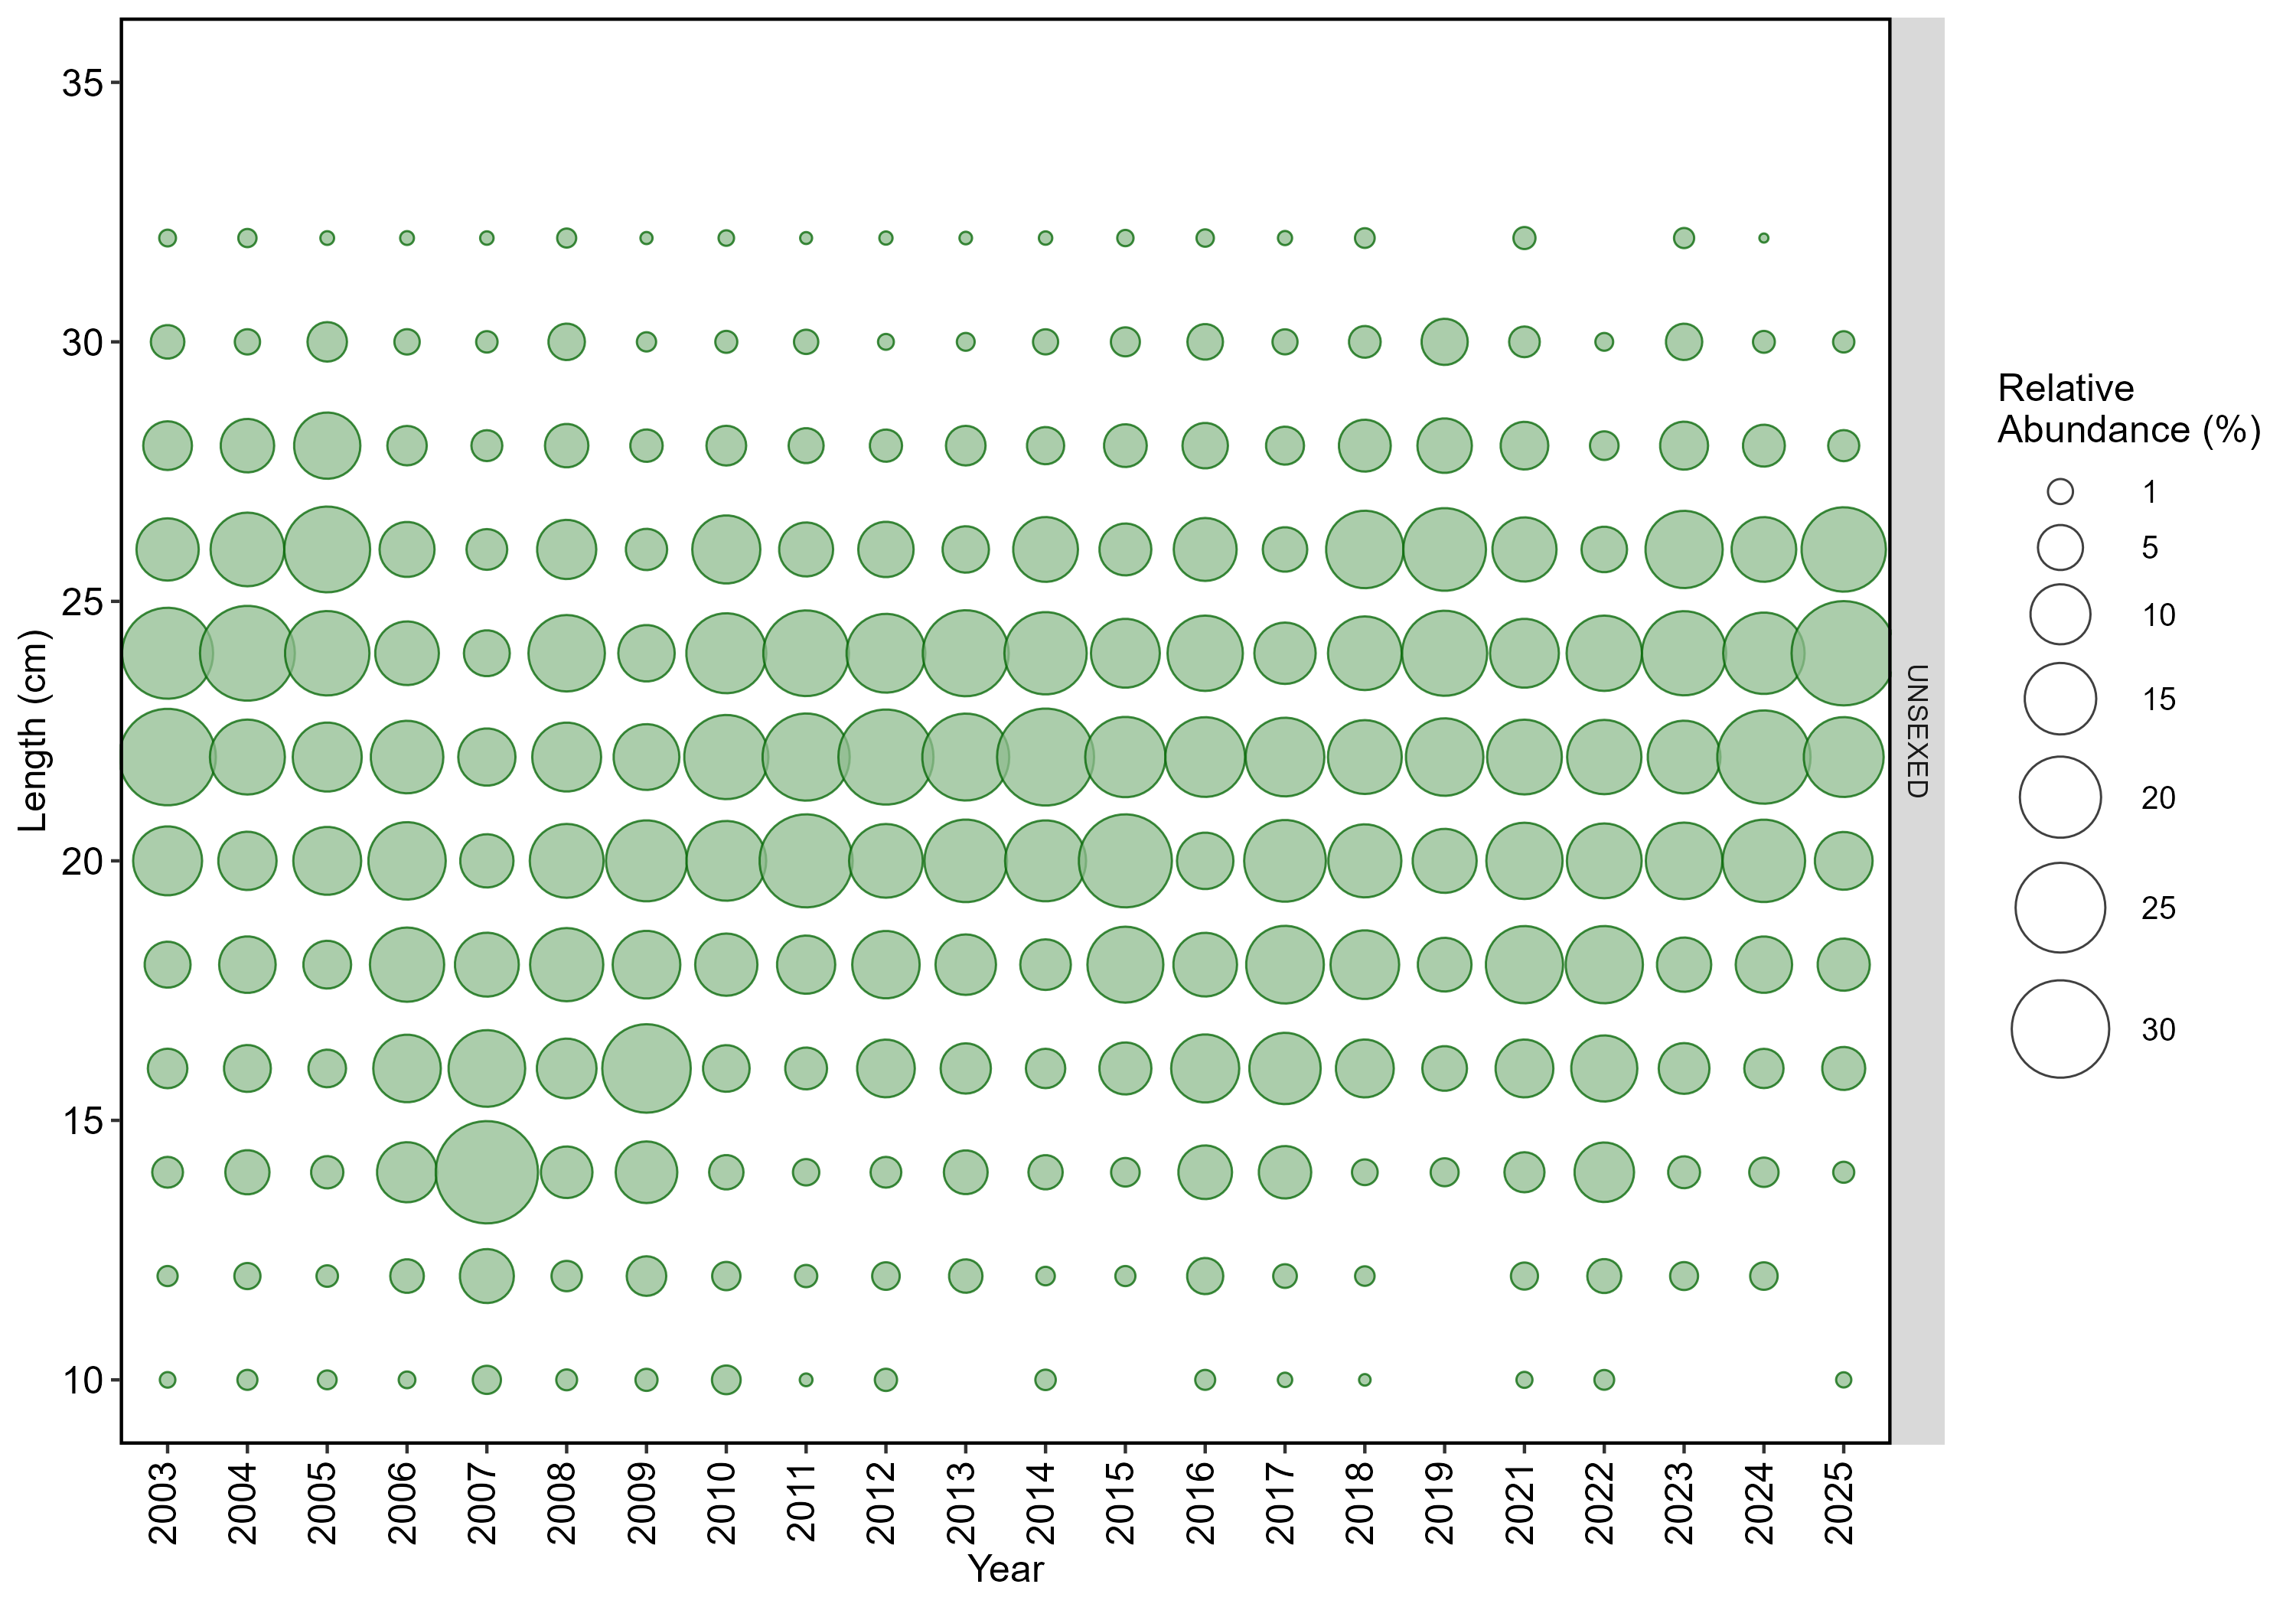
\includegraphics[width=0.95\linewidth,height=\textheight,keepaspectratio]{../plots/wcgbts_comps/plots/rosethorn rockfish_length_frequency_sex_0.png}

}

\caption{Length (cm) compostion data from the NWFSC WCGBTS for rosethorn
rockfish. Size of the circles within a year indicate higher (larger
circles) and lower (smaller circles) proportion observed by length bin.}

\end{figure}%

\newpage{}

\subsection{Rougheye and blackspotted
rockfish}\label{rougheye-and-blackspotted-rockfish}

The most recent assessment of rougheye and blackspotted rockfish was a
benchmark assessment conducted in 2025. Across available data, rougheye
and blackspotted rockfish have been observed and sampled by the NWFSC
WCGBTS. The NWFSC HKLS observed rougheye and blackspotted rockfish at an
average of 0 sets per year. The NWFSC WCGBTS observed rougheye and
blackspotted rockfish on an average of 27 tows per year. For this
species, a total of 549 maturity samples have been collected coastwide
(regardless of stock area), with 549 read maturities.

\begingroup\fontsize{10}{12}\selectfont
\begingroup\fontsize{10}{12}\selectfont

\begin{longtable}[t]{>{\raggedleft\arraybackslash}p{2cm}>{\raggedleft\arraybackslash}p{3.5cm}>{\raggedleft\arraybackslash}p{2cm}>{\raggedleft\arraybackslash}p{2cm}>{\raggedleft\arraybackslash}p{2cm}}
\caption{\label{tab:unnamed-chunk-533}Total number of available lengths, read ages, and unread age structures by data source and
state for rougheye and blackspotted rockfish.}\\
\toprule
State & Source & Lengths & Ages & Age Structures\\
\midrule
\endfirsthead
\caption[]{Total number of available lengths, read ages, and unread age structures by data source and
state for rougheye and blackspotted rockfish. (\textit{continued)}}\\
\toprule
State & Source & Lengths & Ages & Age Structures\\
\midrule
\endhead

\endfoot
\bottomrule
\endlastfoot
CA & NWFSC HKLS & 1 & 0 & 1\\
CA & NWFSC WCGBTS & 17 & 13 & 3\\
OR & NWFSC WCGBTS & 1,075 & 855 & 55\\
WA & NWFSC WCGBTS & 1,197 & 1,003 & 47\\*
\end{longtable}
\endgroup{}
\endgroup{}

\begin{figure}[H]

{\centering 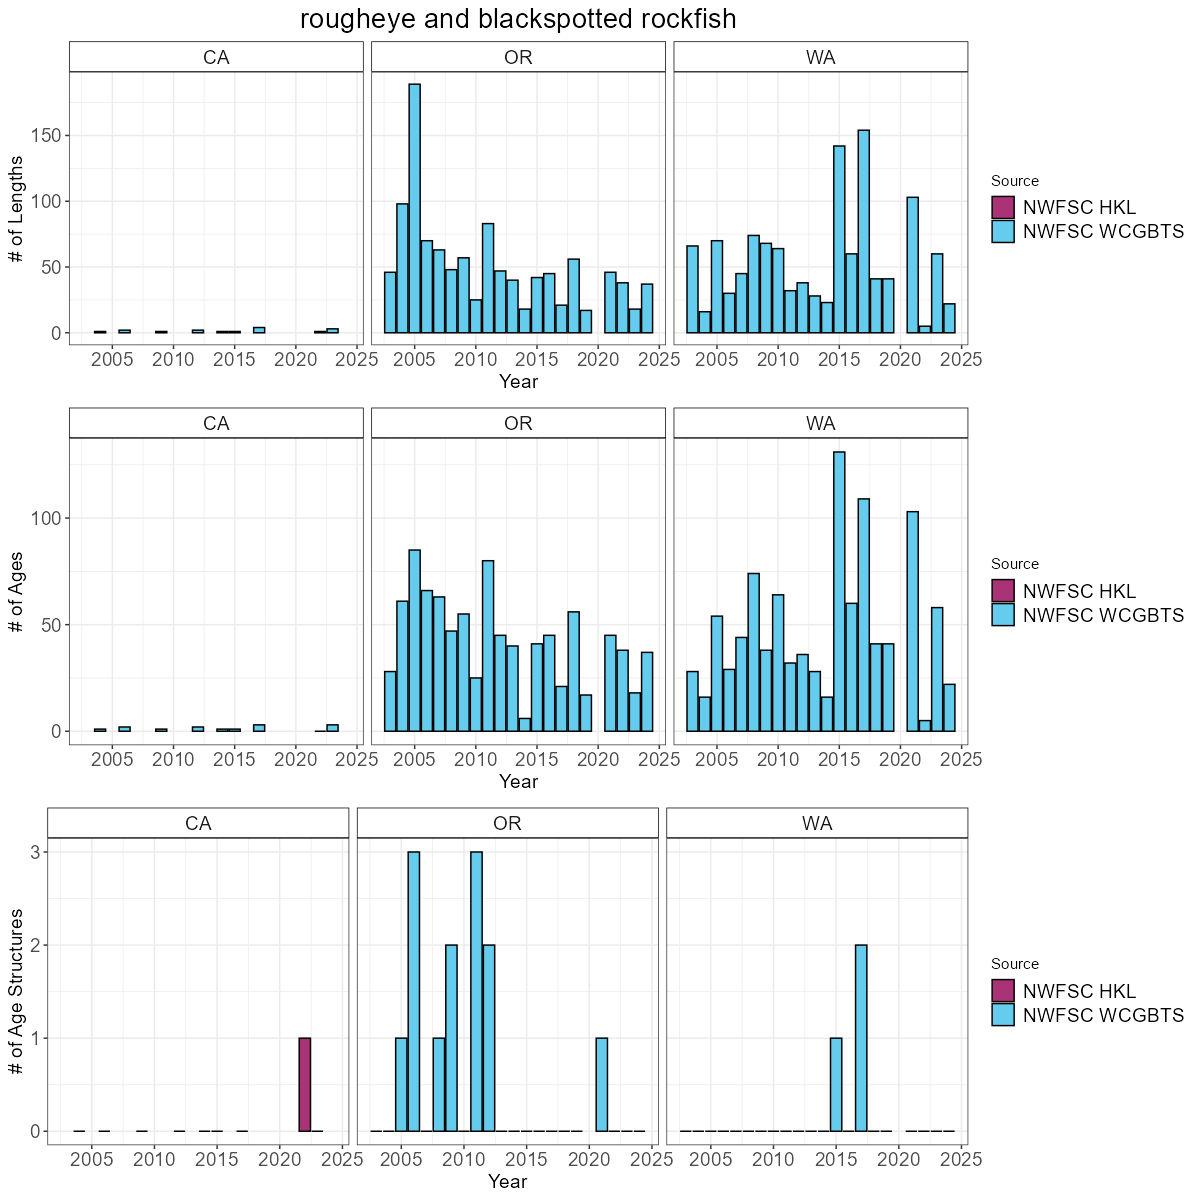
\includegraphics[width=0.95\linewidth,height=\textheight,keepaspectratio]{../plots/state_comparisons/rougheye_and_blackspotted_rockfish_state_compositions.png}

}

\caption{Total number of available lengths, read ages, and unread age
structures by data source by year for rougheye and blackspotted
rockfish. Note the y-axis maximum may differ by data type.}

\end{figure}%

\begin{figure}[H]

{\centering 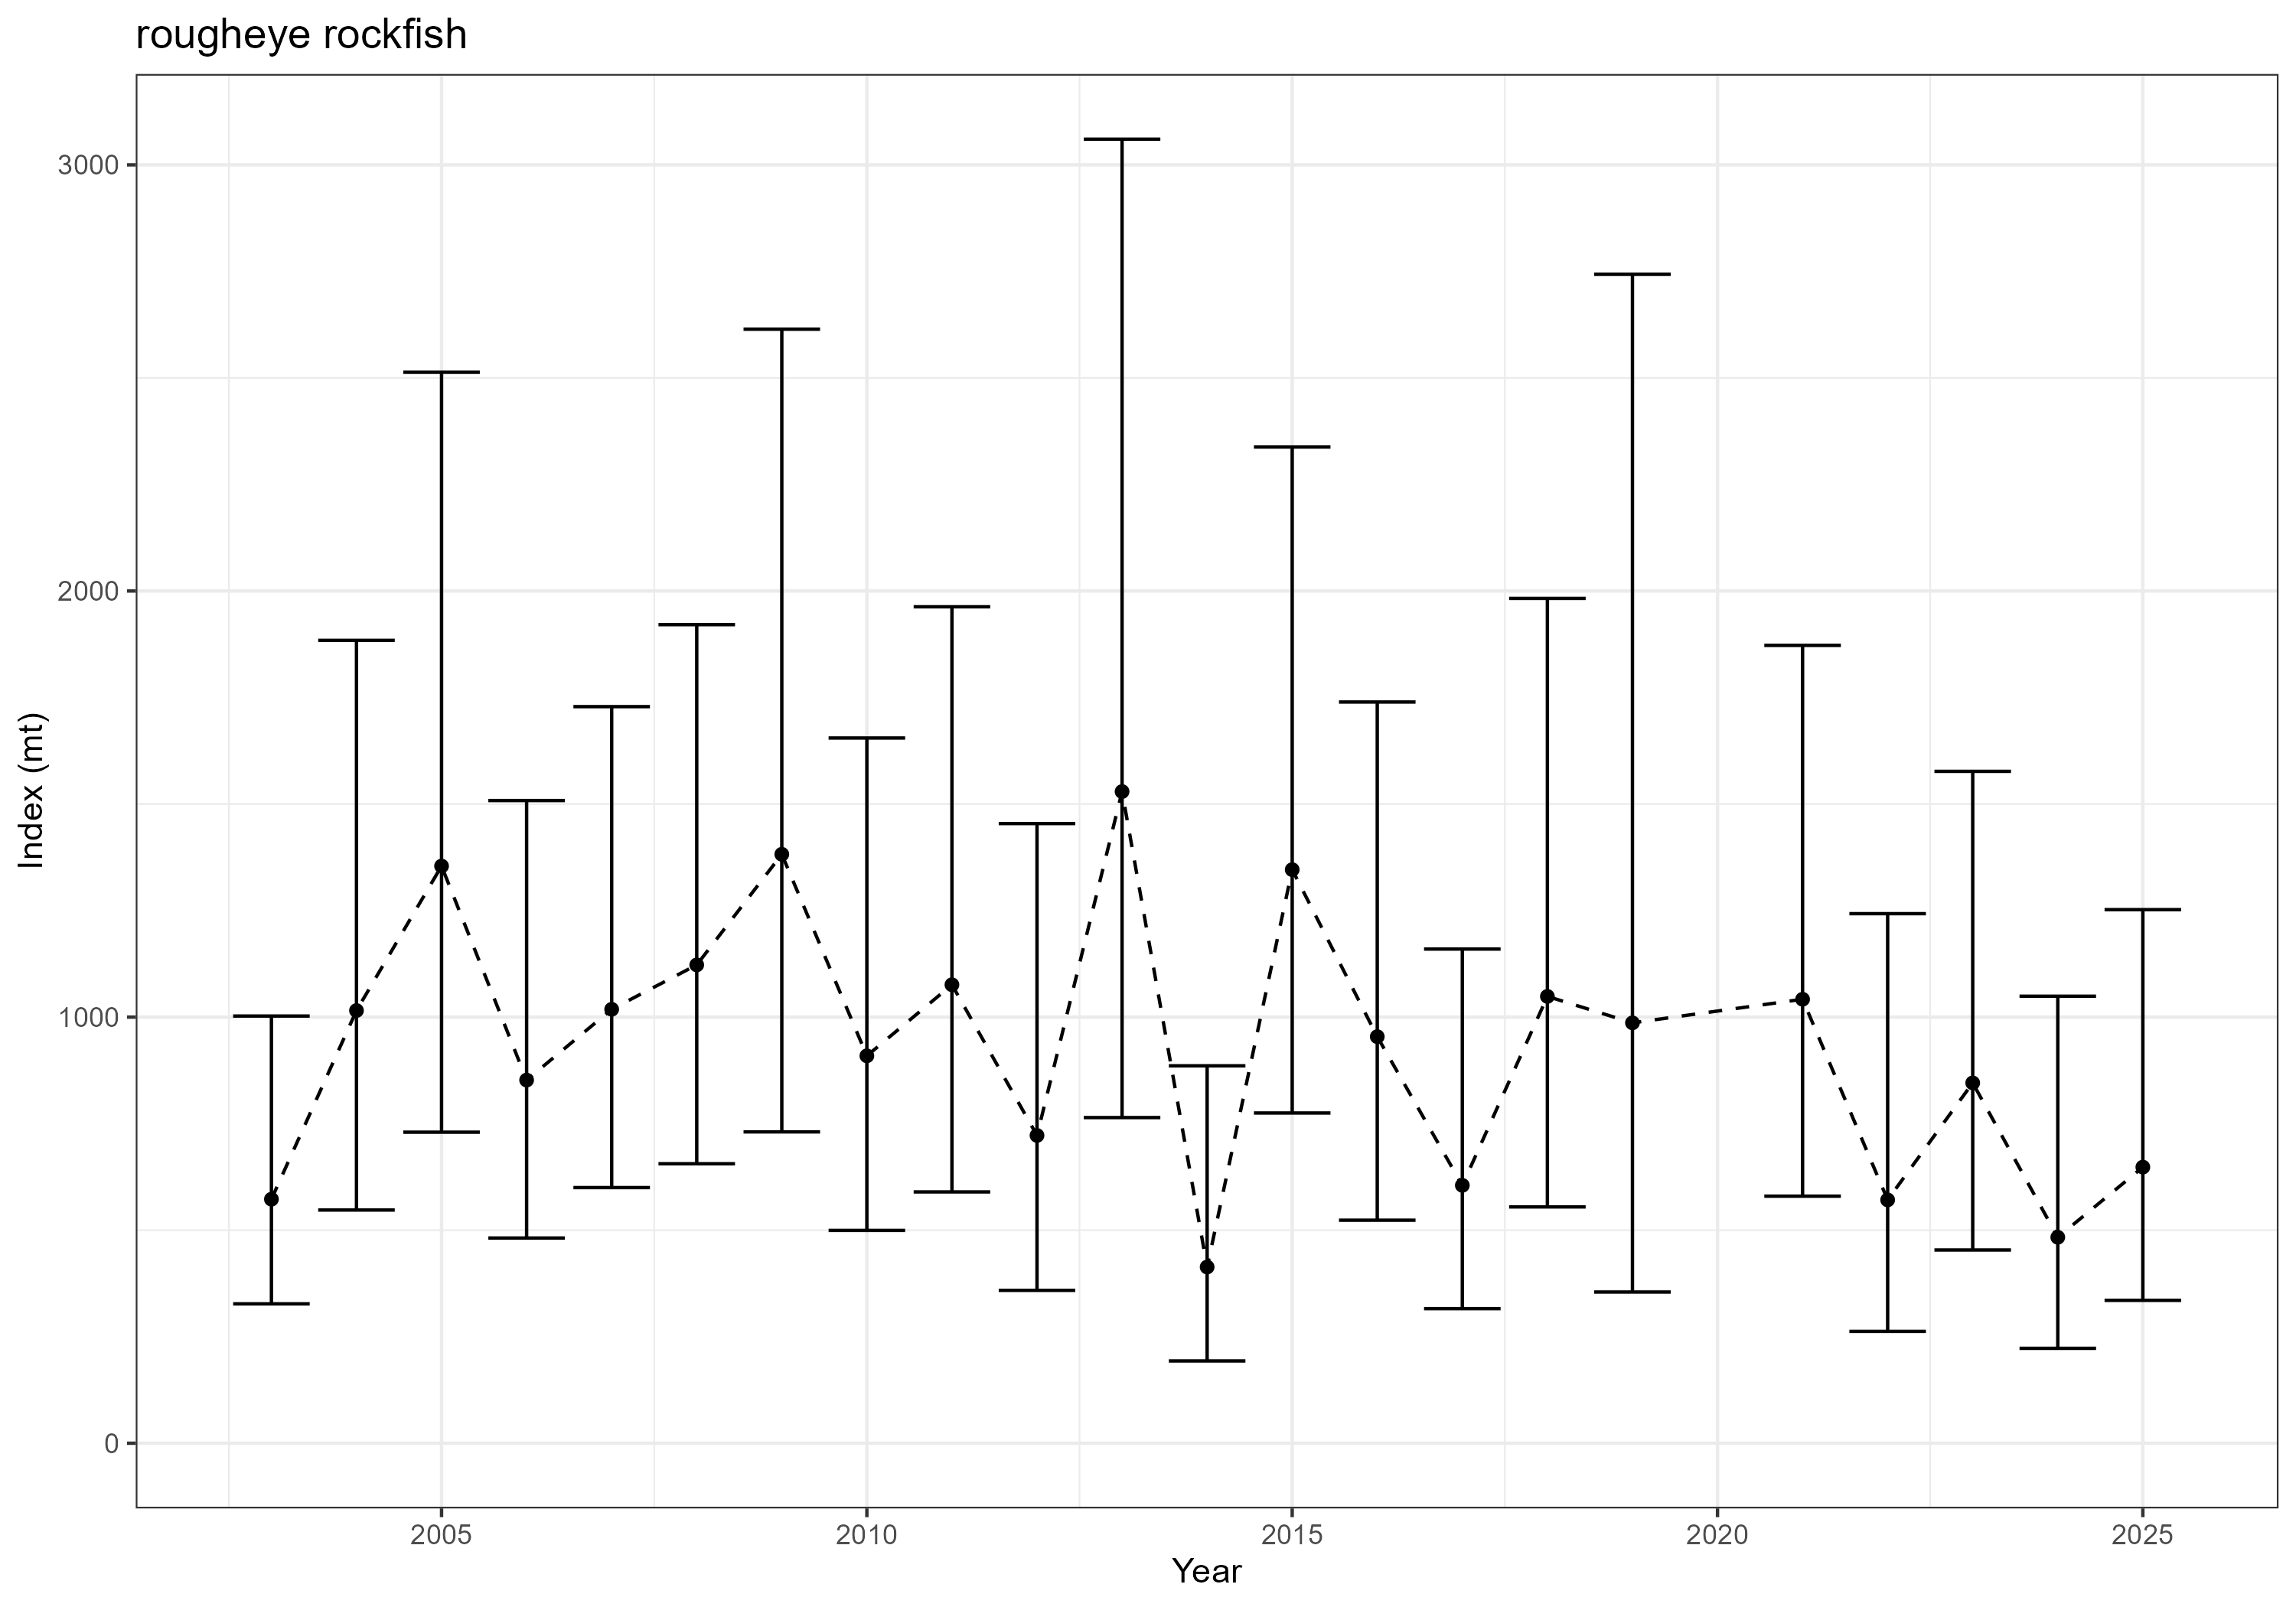
\includegraphics[width=0.95\linewidth,height=\textheight,keepaspectratio]{../plots/wcgbts_indices/rougheye_and_blackspotted_rockfish_index.png}

}

\caption{Estimated relative index of abundance for rougheye and
blackspotted rockfish from the NWFSC WCGBTS.}

\end{figure}%

\begin{figure}[H]

{\centering 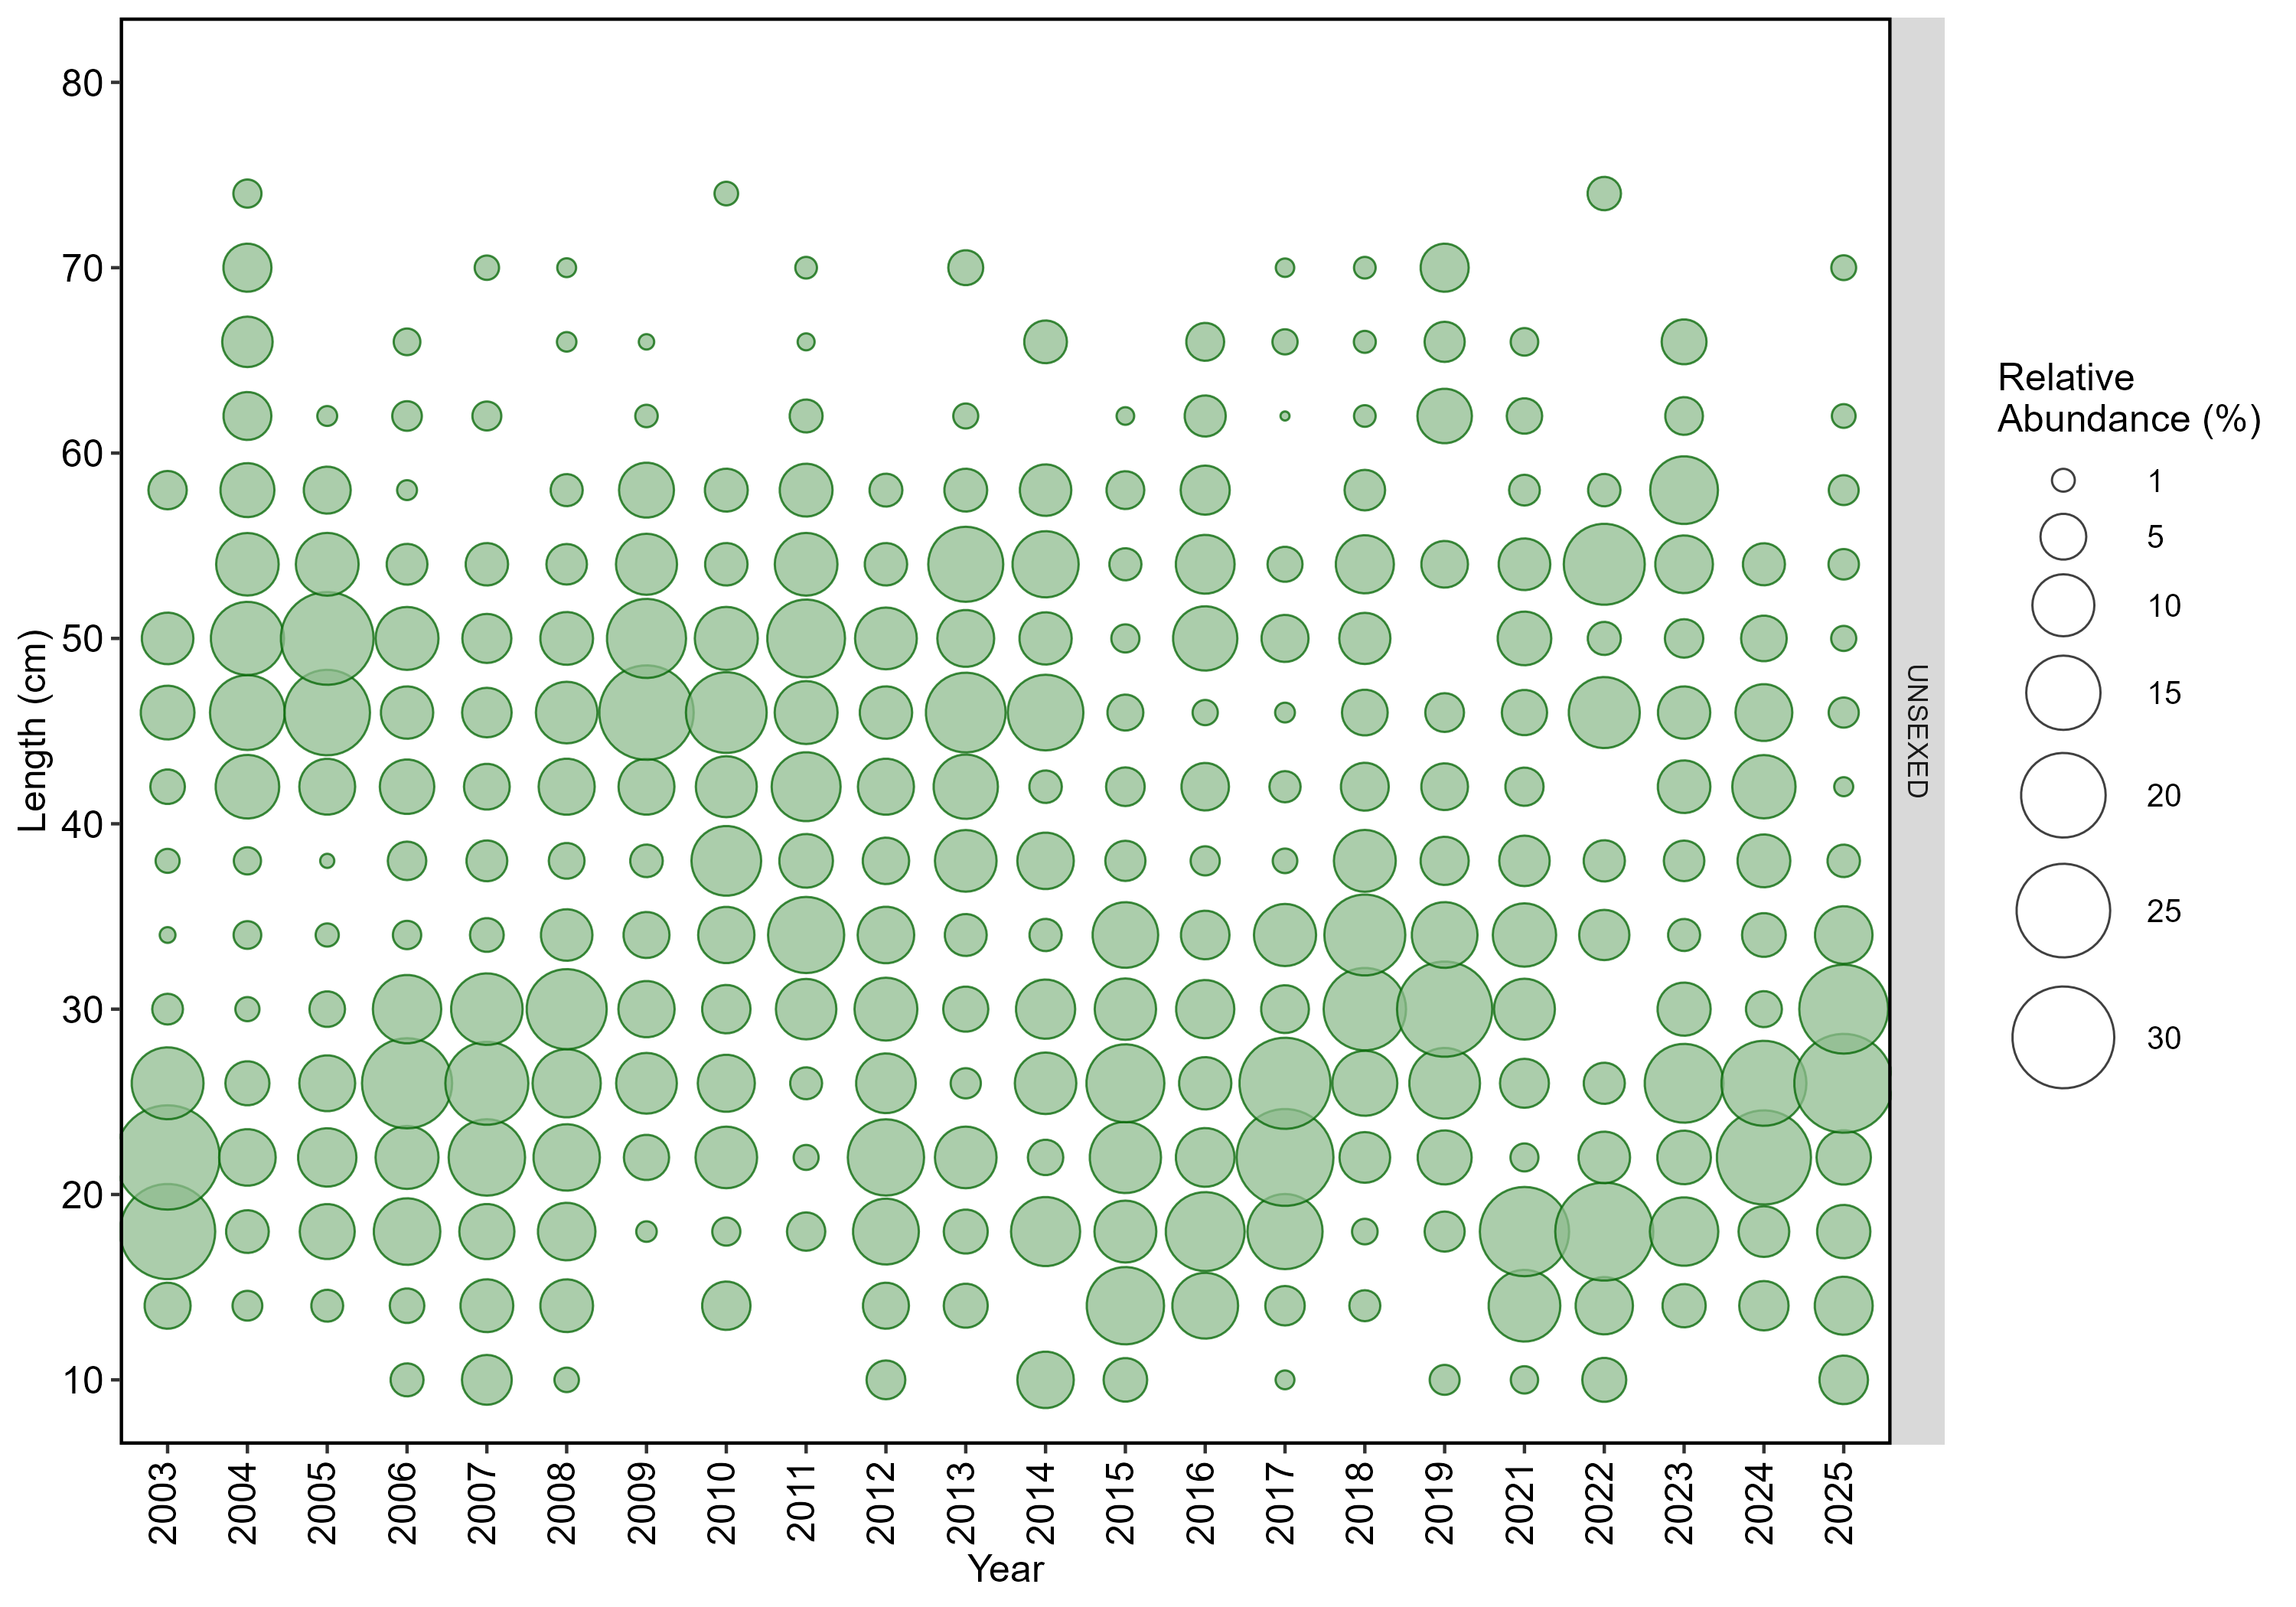
\includegraphics[width=0.95\linewidth,height=\textheight,keepaspectratio]{../plots/wcgbts_comps/plots/rougheye and blackspotted rockfish_length_frequency_sex_0.png}

}

\caption{Length (cm) compostion data from the NWFSC WCGBTS for rougheye
and blackspotted rockfish. Size of the circles within a year indicate
higher (larger circles) and lower (smaller circles) proportion observed
by length bin.}

\end{figure}%

\newpage{}

\subsection{Sablefish}\label{sablefish}

The most recent assessment of sablefish was a benchmark assessment
conducted in 2025. Across available data, sablefish have been observed
and sampled by the NWFSC WCGBTS. The NWFSC WCGBTS observed sablefish on
an average of 427 tows per year. For this species, a total of 1312
maturity samples have been collected coastwide (regardless of stock
area), with 1157 read maturities.

\begingroup\fontsize{10}{12}\selectfont
\begingroup\fontsize{10}{12}\selectfont

\begin{longtable}[t]{>{\raggedleft\arraybackslash}p{2cm}>{\raggedleft\arraybackslash}p{3.5cm}>{\raggedleft\arraybackslash}p{2cm}>{\raggedleft\arraybackslash}p{2cm}>{\raggedleft\arraybackslash}p{2cm}}
\caption{\label{tab:unnamed-chunk-550}Total number of available lengths, read ages, and unread age structures by data source and
state for sablefish.}\\
\toprule
State & Source & Lengths & Ages & Age Structures\\
\midrule
\endfirsthead
\caption[]{Total number of available lengths, read ages, and unread age structures by data source and
state for sablefish. (\textit{continued)}}\\
\toprule
State & Source & Lengths & Ages & Age Structures\\
\midrule
\endhead

\endfoot
\bottomrule
\endlastfoot
CA & NWFSC WCGBTS & 53,722 & 13,650 & 6,899\\
OR & NWFSC WCGBTS & 39,178 & 9,952 & 4,880\\
WA & NWFSC WCGBTS & 14,048 & 3,931 & 1,774\\*
\end{longtable}
\endgroup{}
\endgroup{}

\begin{figure}[H]

{\centering 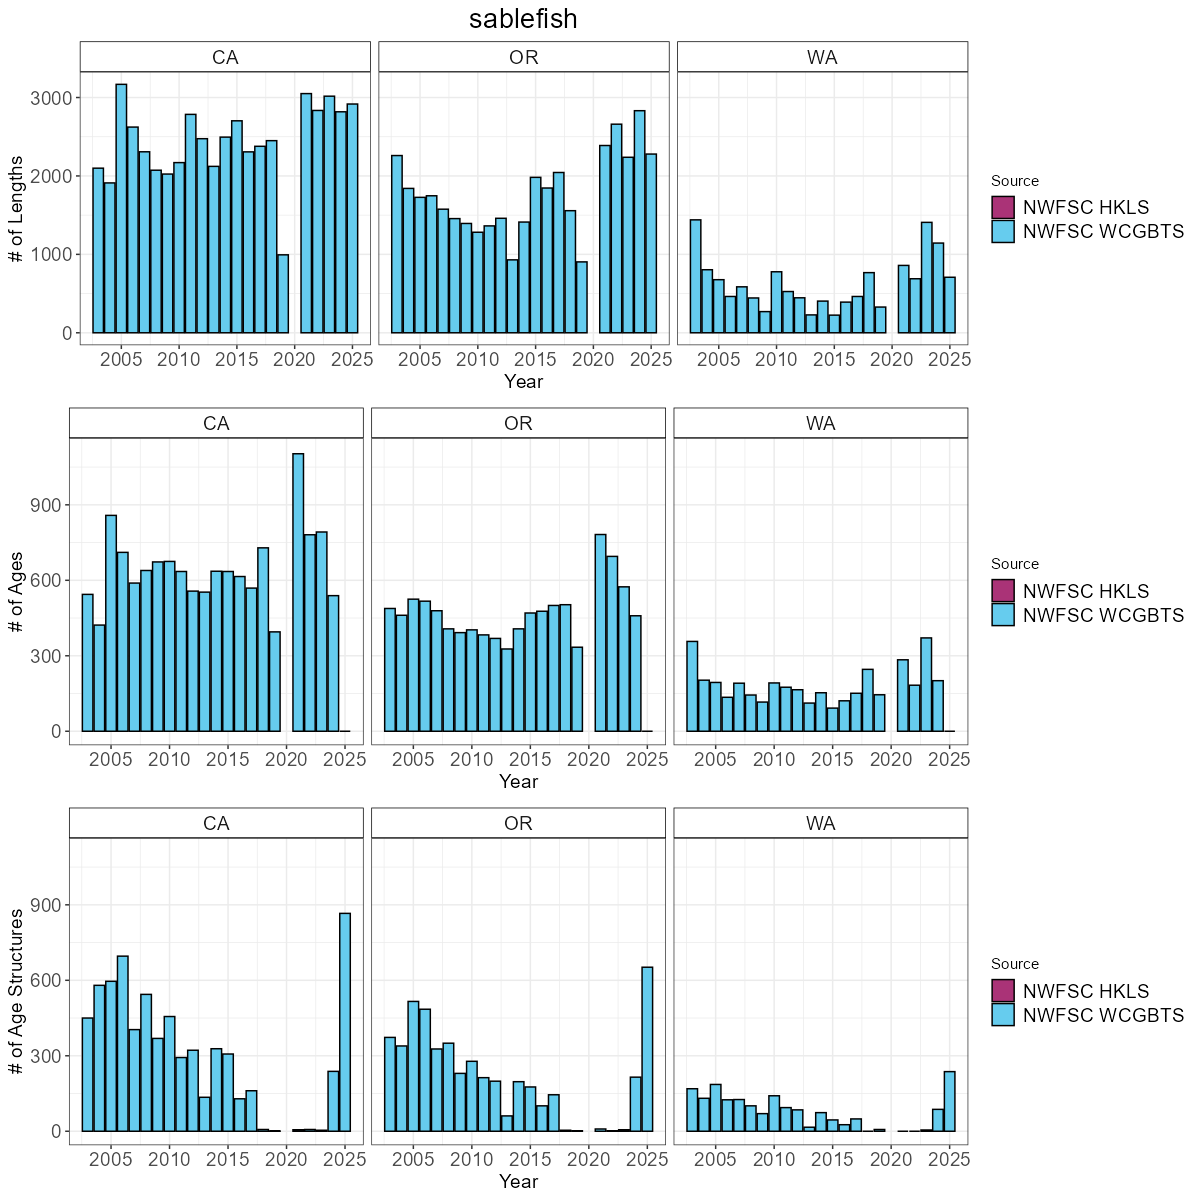
\includegraphics[width=0.95\linewidth,height=\textheight,keepaspectratio]{../plots/state_comparisons/sablefish_state_compositions.png}

}

\caption{Total number of available lengths, read ages, and unread age
structures by data source by year for sablefish. Note the y-axis maximum
may differ by data type.}

\end{figure}%

\begin{figure}[H]

{\centering 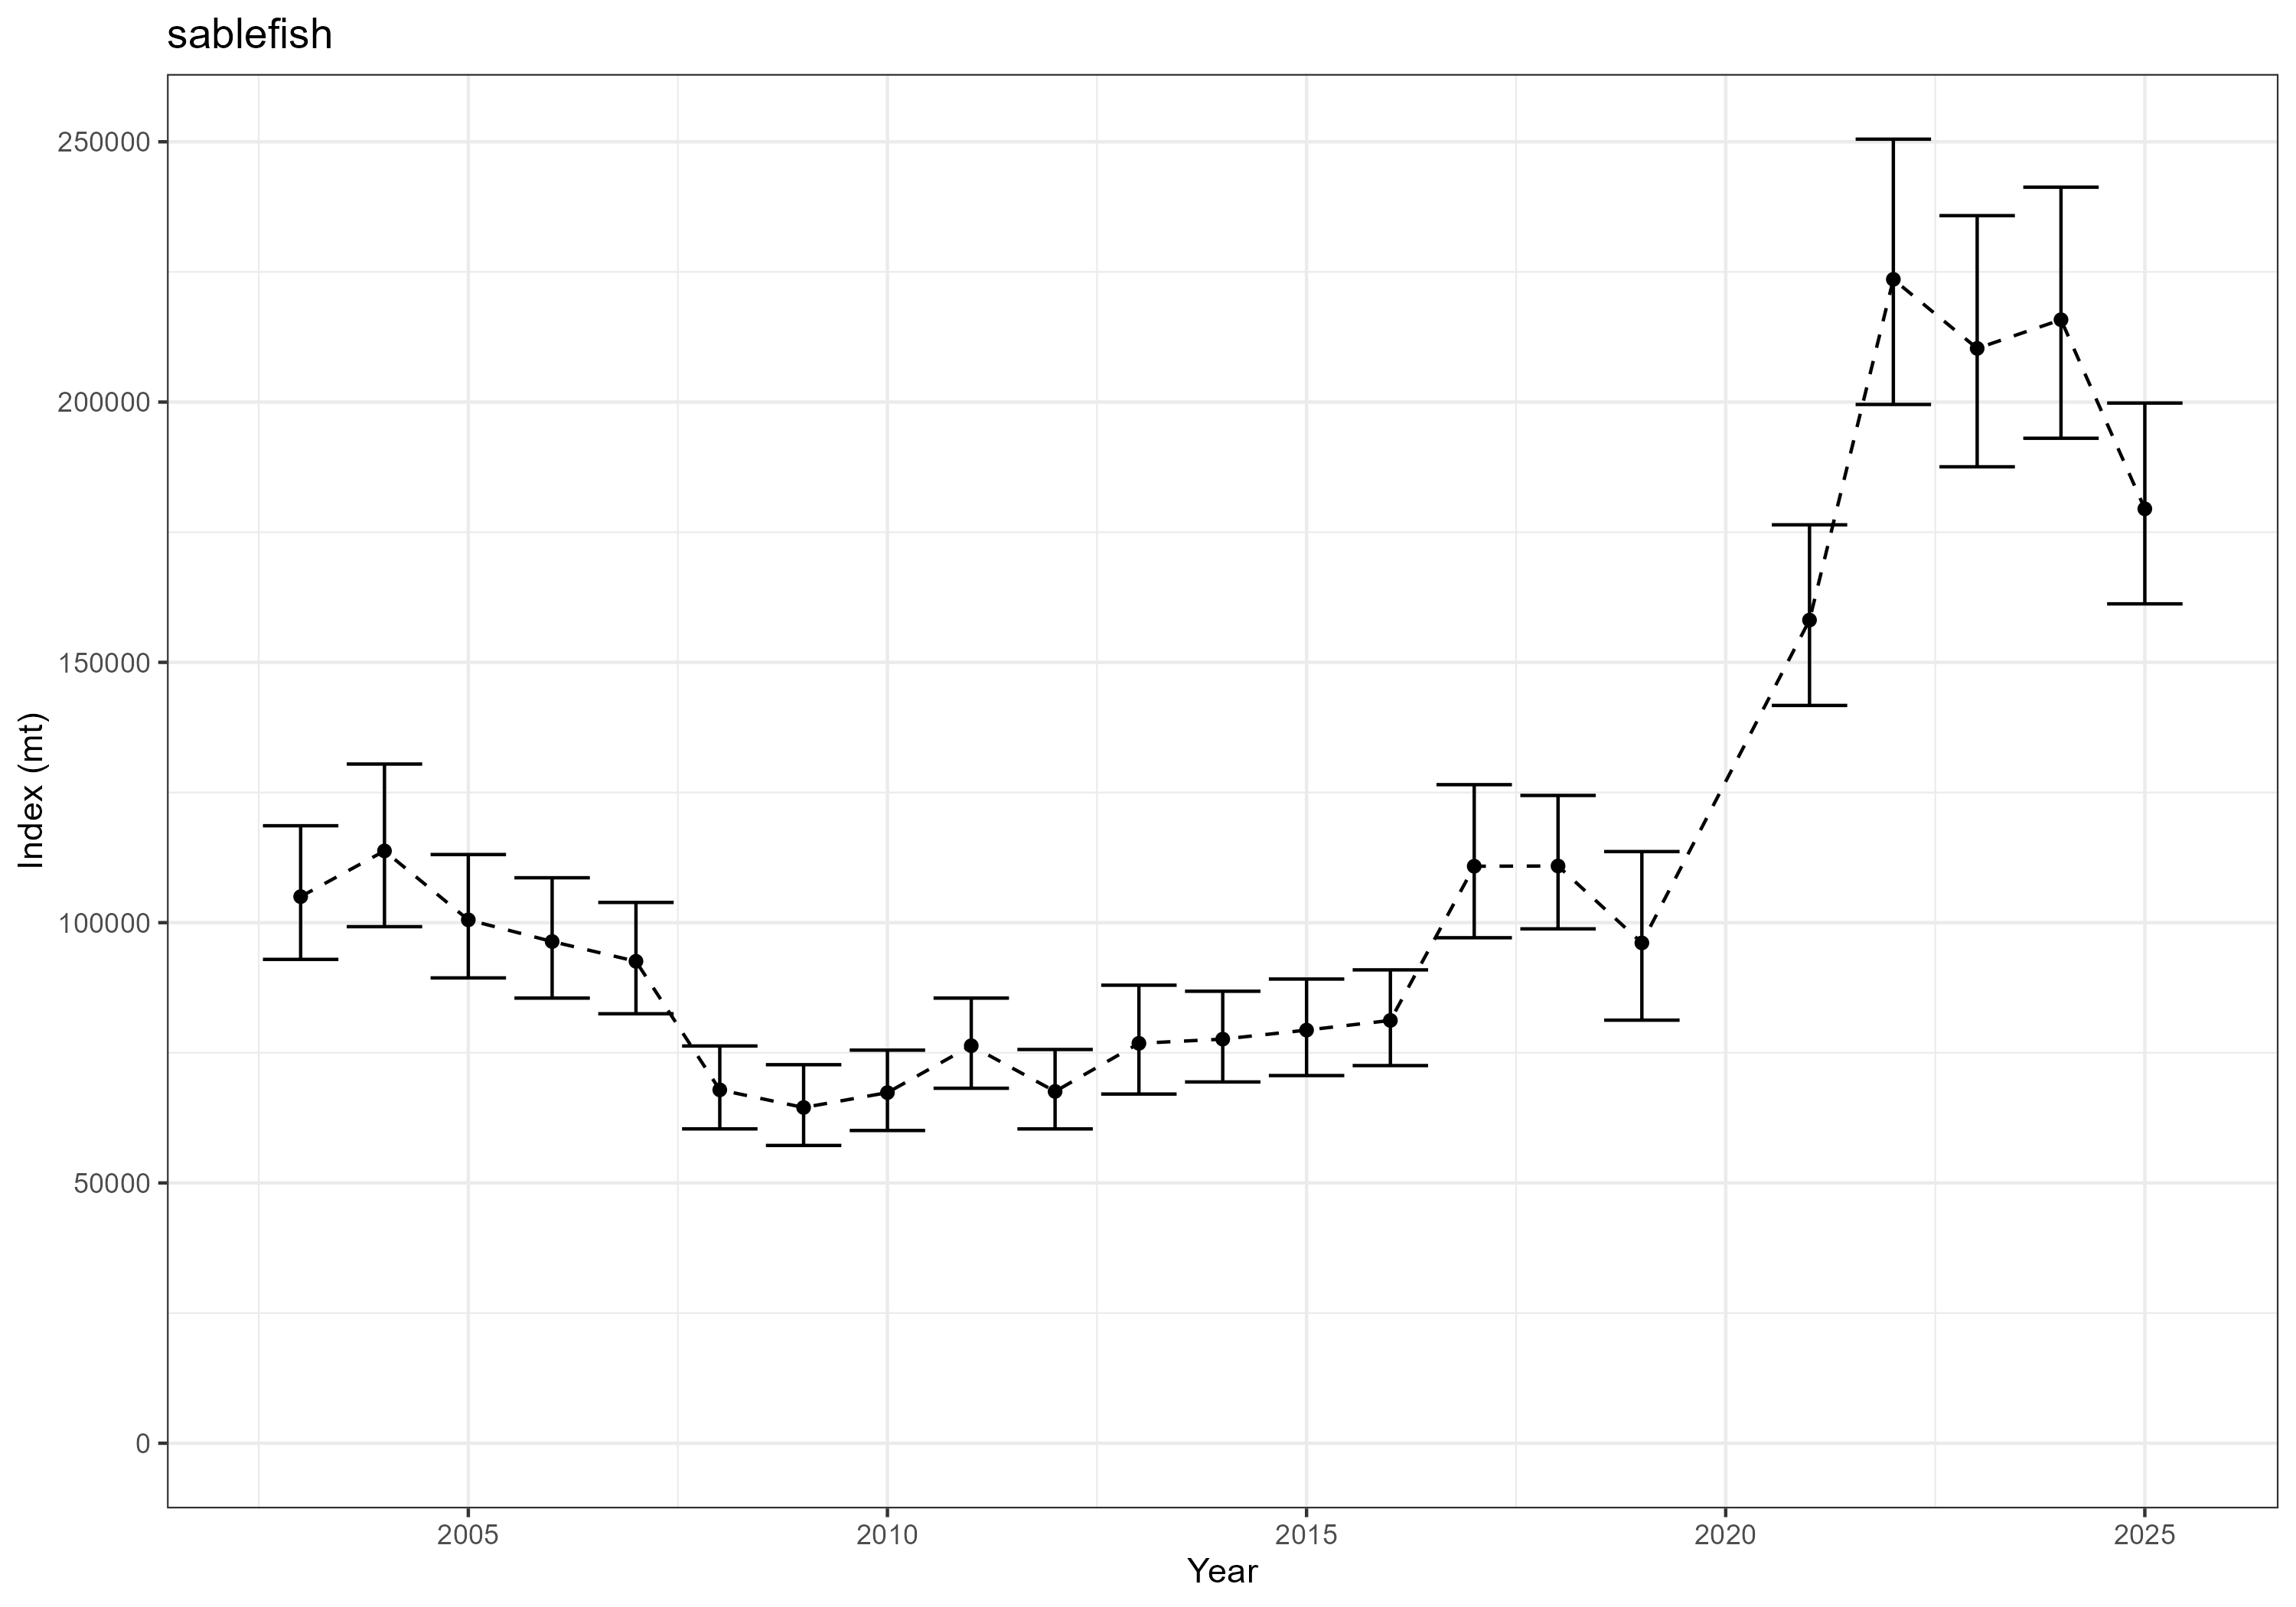
\includegraphics[width=0.95\linewidth,height=\textheight,keepaspectratio]{../plots/wcgbts_indices/sablefish_index.png}

}

\caption{Estimated relative index of abundance for sablefish from the
NWFSC WCGBTS.}

\end{figure}%

\begin{figure}[H]

{\centering 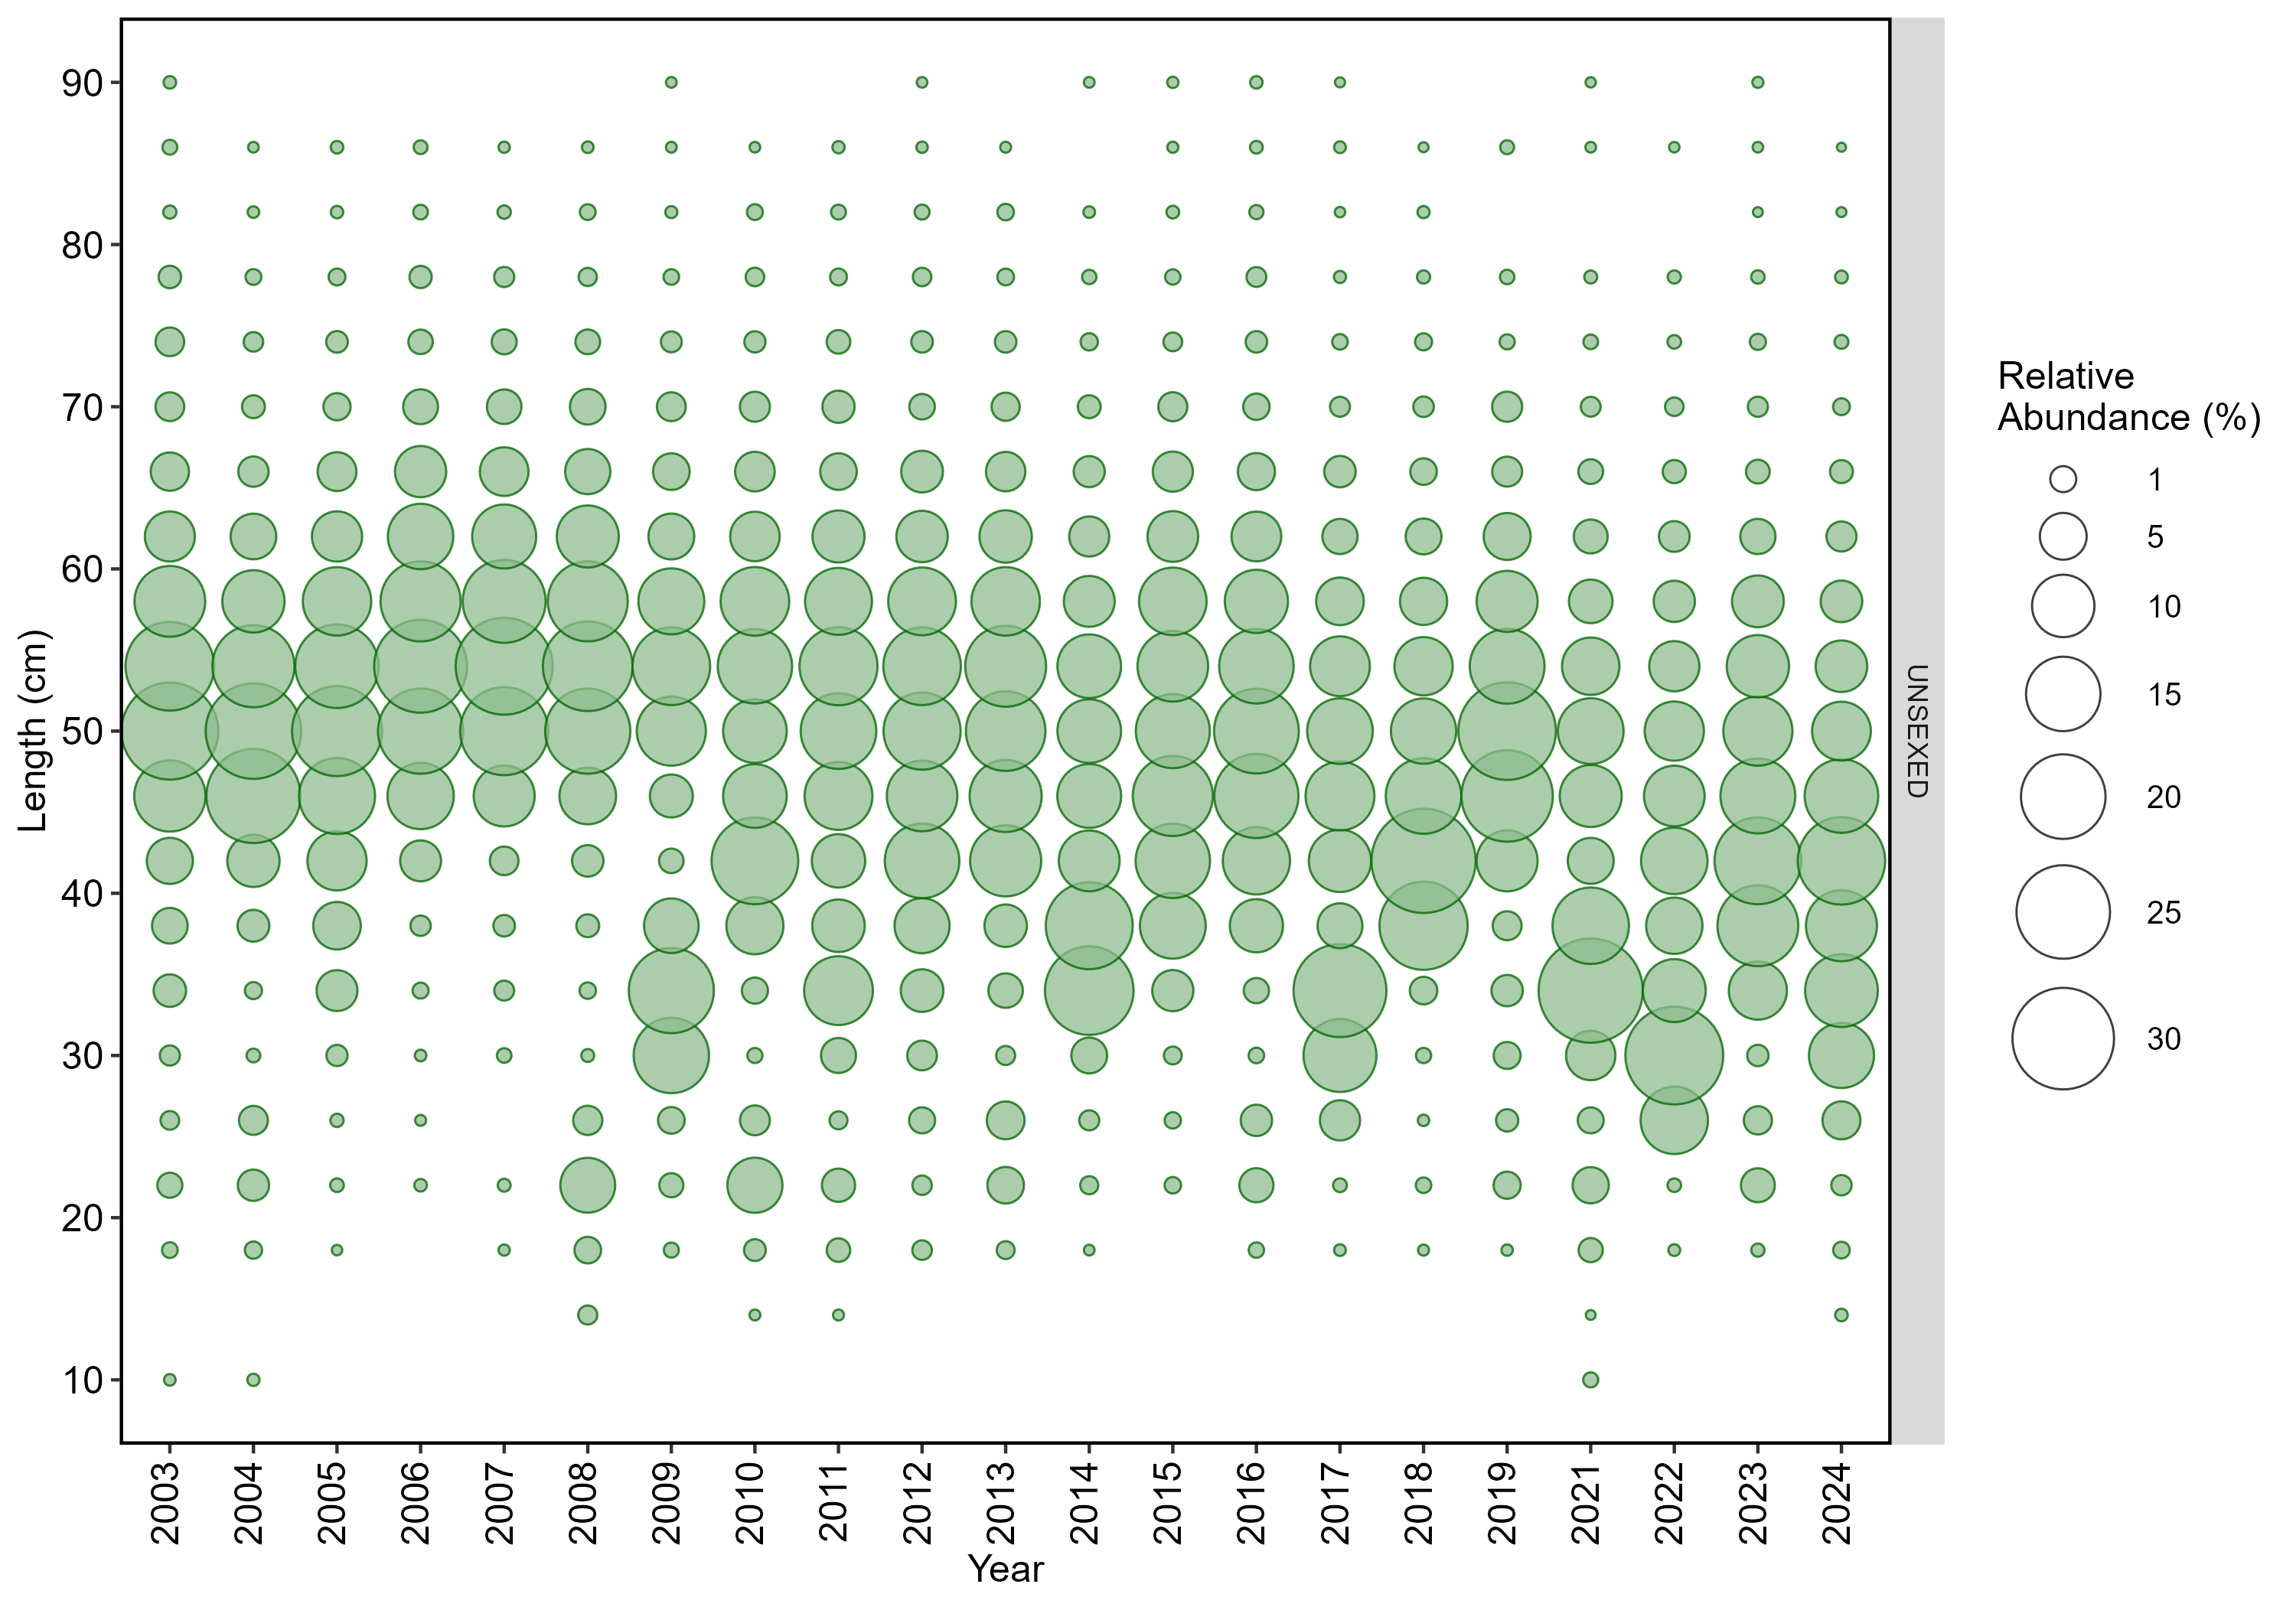
\includegraphics[width=0.95\linewidth,height=\textheight,keepaspectratio]{../plots/wcgbts_comps/plots/sablefish_length_frequency_sex_0.png}

}

\caption{Length (cm) compostion data from the NWFSC WCGBTS for
sablefish. Size of the circles within a year indicate higher (larger
circles) and lower (smaller circles) proportion observed by length bin.}

\end{figure}%

\newpage{}

\subsection{Sharpchin rockfish}\label{sharpchin-rockfish}

The most recent assessment of sharpchin rockfish was a data-moderate
assessment conducted in 2013. Across available data, sharpchin rockfish
have been observed and sampled by both the NWFSC HKLS and WCGBTS. The
NWFSC HKLS observed sharpchin rockfish at an average of 0 sets per year.
The NWFSC WCGBTS observed sharpchin rockfish on an average of 43 tows
per year. For this species, a total of 0 maturity samples have been
collected coastwide (regardless of stock area).

\begingroup\fontsize{10}{12}\selectfont
\begingroup\fontsize{10}{12}\selectfont

\begin{longtable}[t]{>{\raggedleft\arraybackslash}p{2cm}>{\raggedleft\arraybackslash}p{3.5cm}>{\raggedleft\arraybackslash}p{2cm}>{\raggedleft\arraybackslash}p{2cm}>{\raggedleft\arraybackslash}p{2cm}}
\caption{\label{tab:unnamed-chunk-567}Total number of available lengths, read ages, and unread age structures by data source and
state for sharpchin rockfish.}\\
\toprule
State & Source & Lengths & Ages & Age Structures\\
\midrule
\endfirsthead
\caption[]{Total number of available lengths, read ages, and unread age structures by data source and
state for sharpchin rockfish. (\textit{continued)}}\\
\toprule
State & Source & Lengths & Ages & Age Structures\\
\midrule
\endhead

\endfoot
\bottomrule
\endlastfoot
CA & NWFSC HKLS & 13 & 0 & 13\\
CA & NWFSC WCGBTS & 3,842 & 0 & 1,958\\
OR & NWFSC WCGBTS & 10,417 & 0 & 4,350\\
WA & NWFSC WCGBTS & 7,048 & 0 & 3,200\\*
\end{longtable}
\endgroup{}
\endgroup{}

\begin{figure}[H]

{\centering 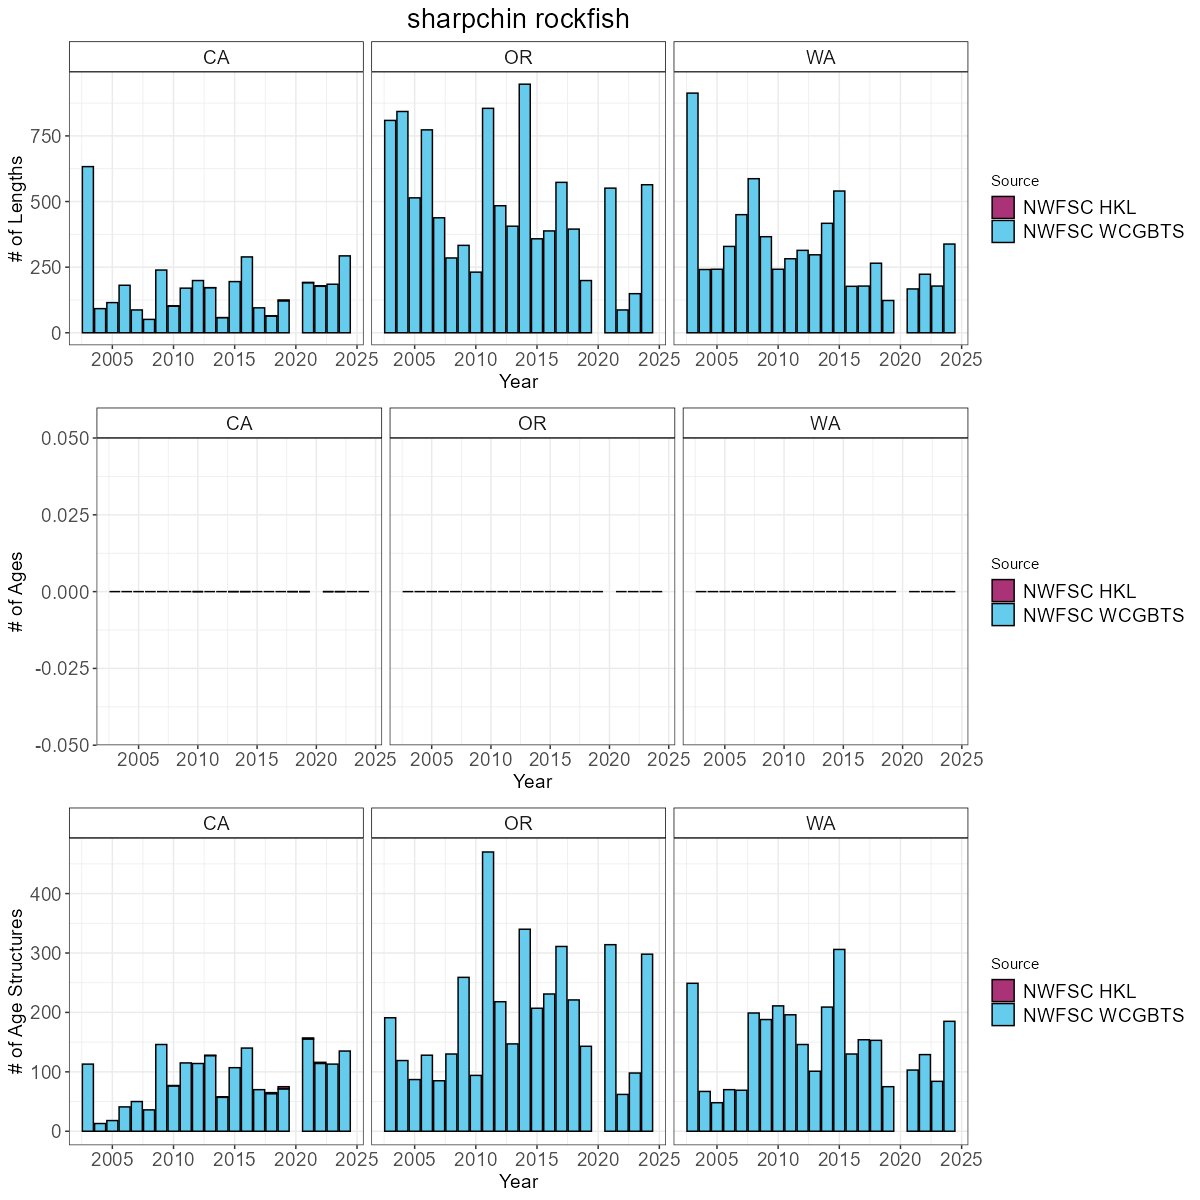
\includegraphics[width=0.95\linewidth,height=\textheight,keepaspectratio]{../plots/state_comparisons/sharpchin_rockfish_state_compositions.png}

}

\caption{Total number of available lengths, read ages, and unread age
structures by data source by year for sharpchin rockfish. Note the
y-axis maximum may differ by data type.}

\end{figure}%

\begin{figure}[H]

{\centering 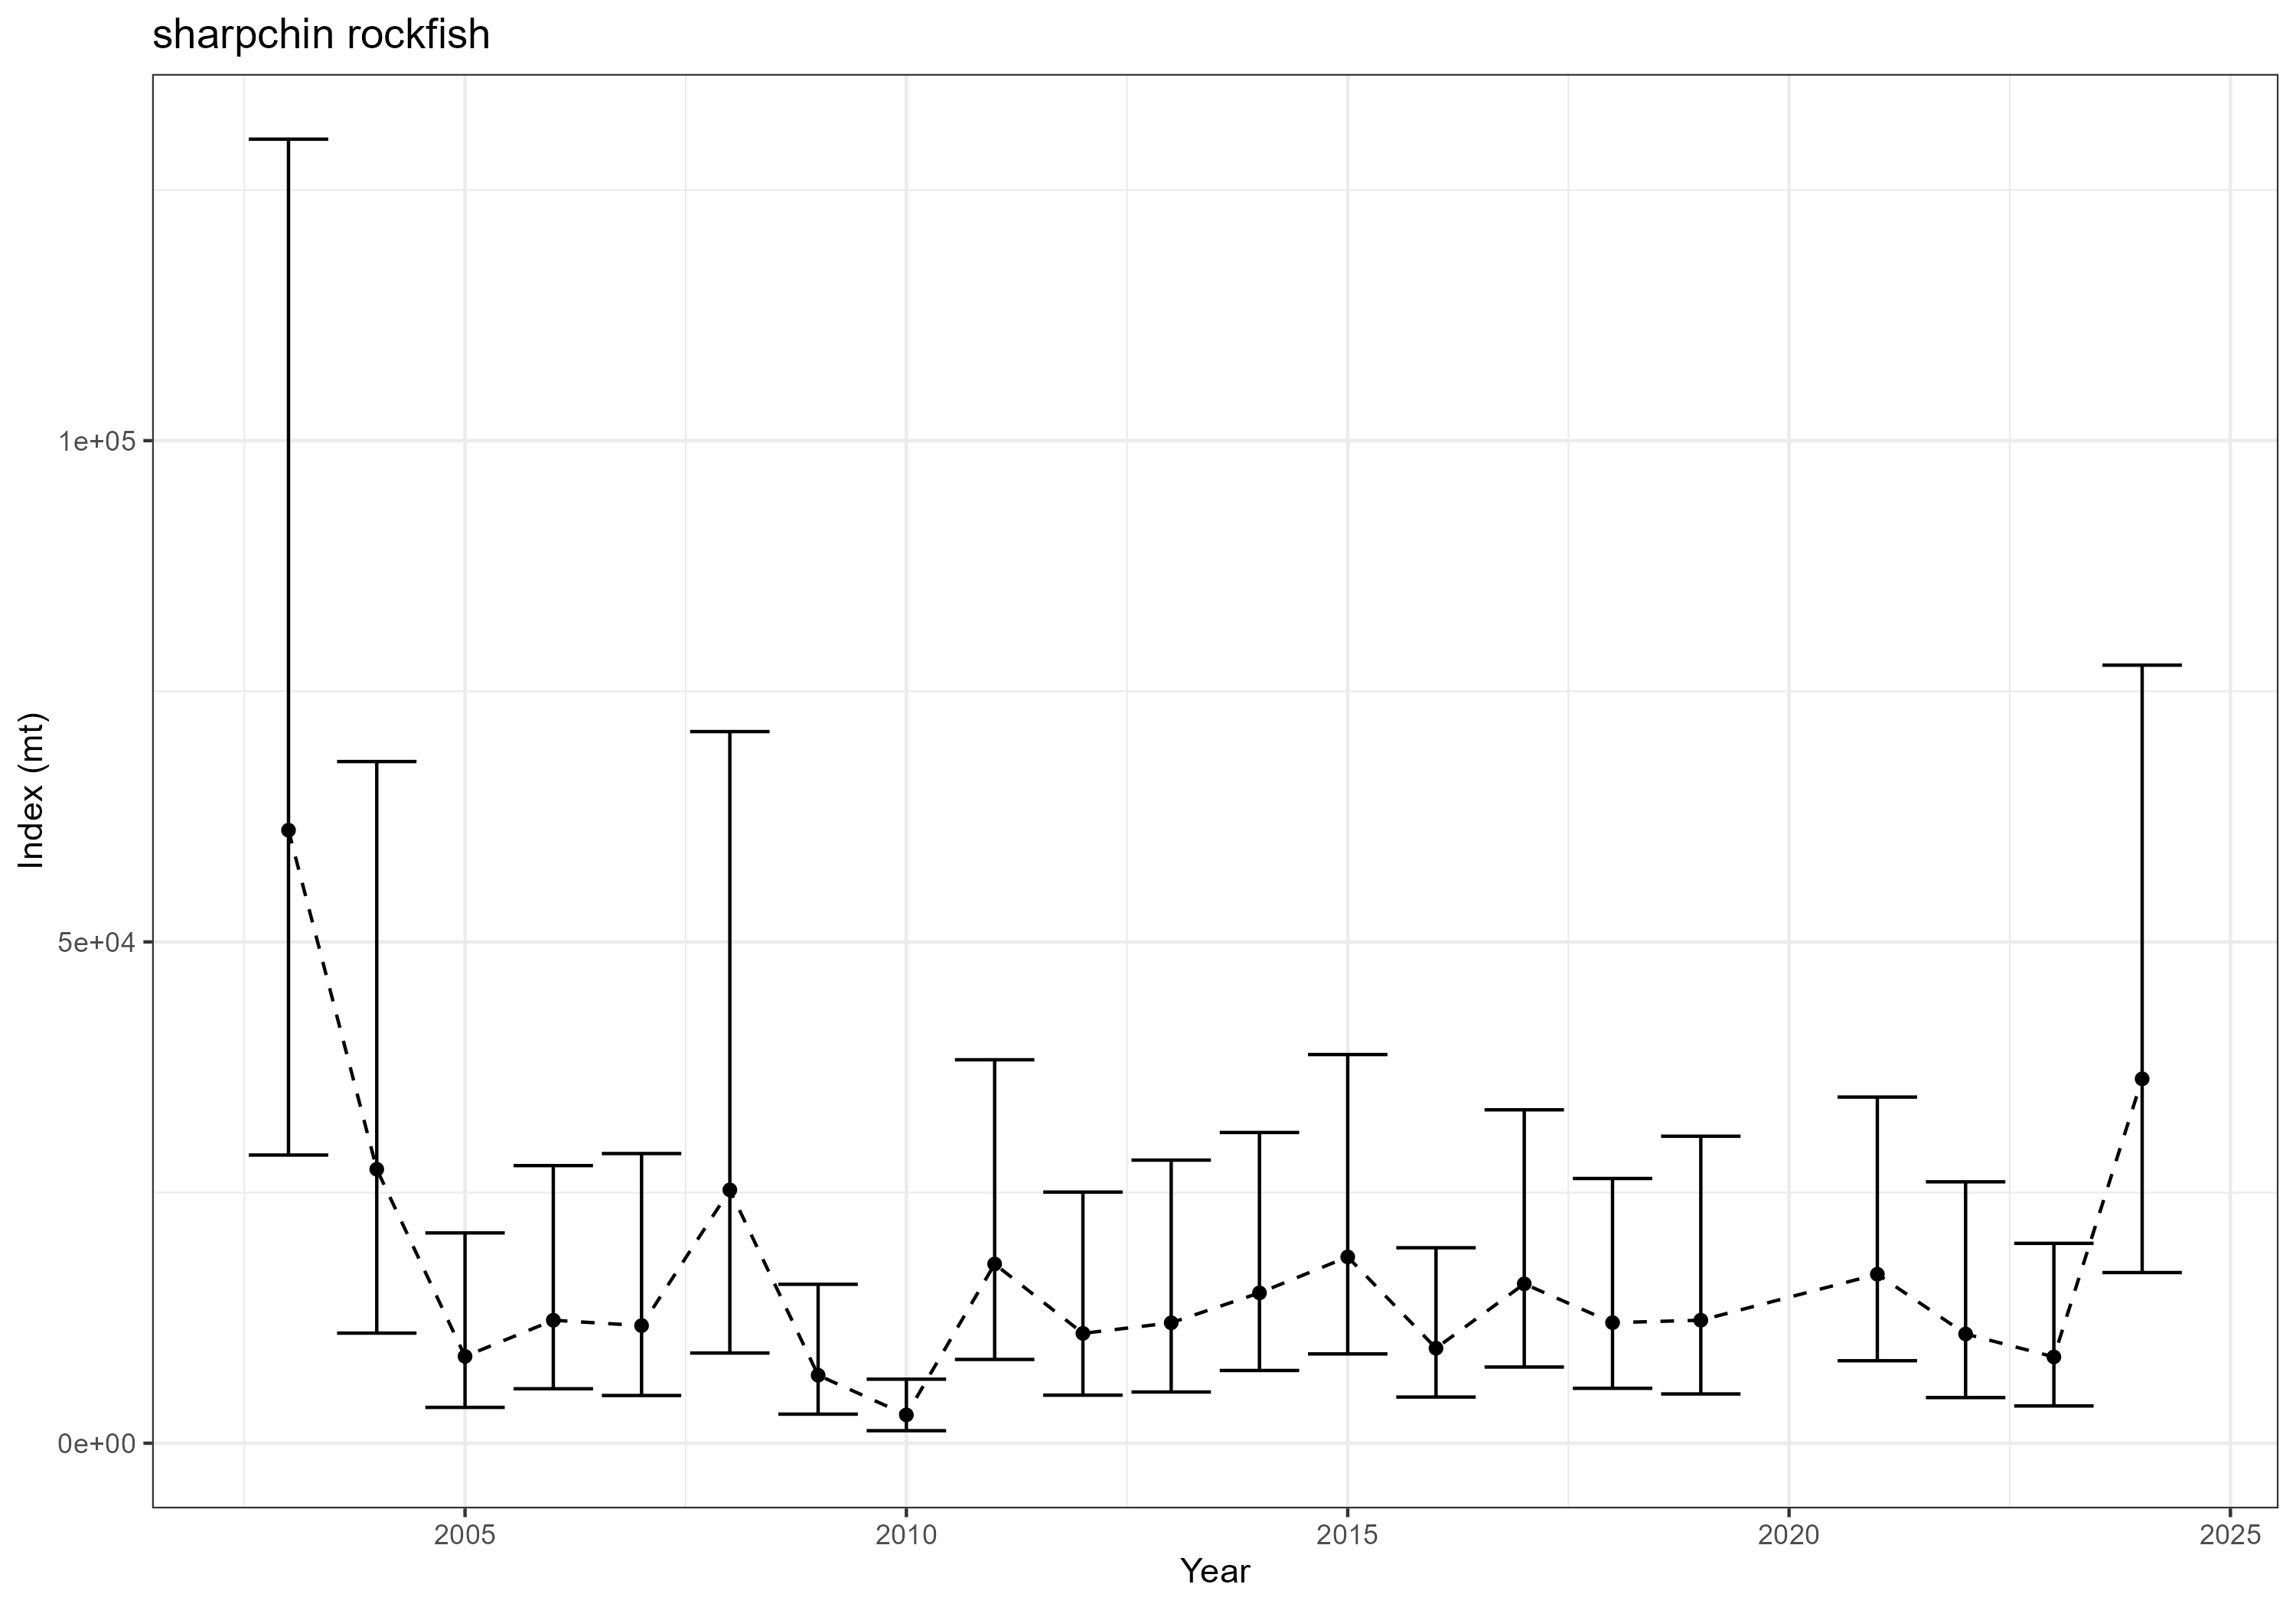
\includegraphics[width=0.95\linewidth,height=\textheight,keepaspectratio]{../plots/wcgbts_indices/sharpchin_rockfish_index.png}

}

\caption{Estimated relative index of abundance for sharpchin rockfish
from the NWFSC WCGBTS.}

\end{figure}%

\begin{figure}[H]

{\centering 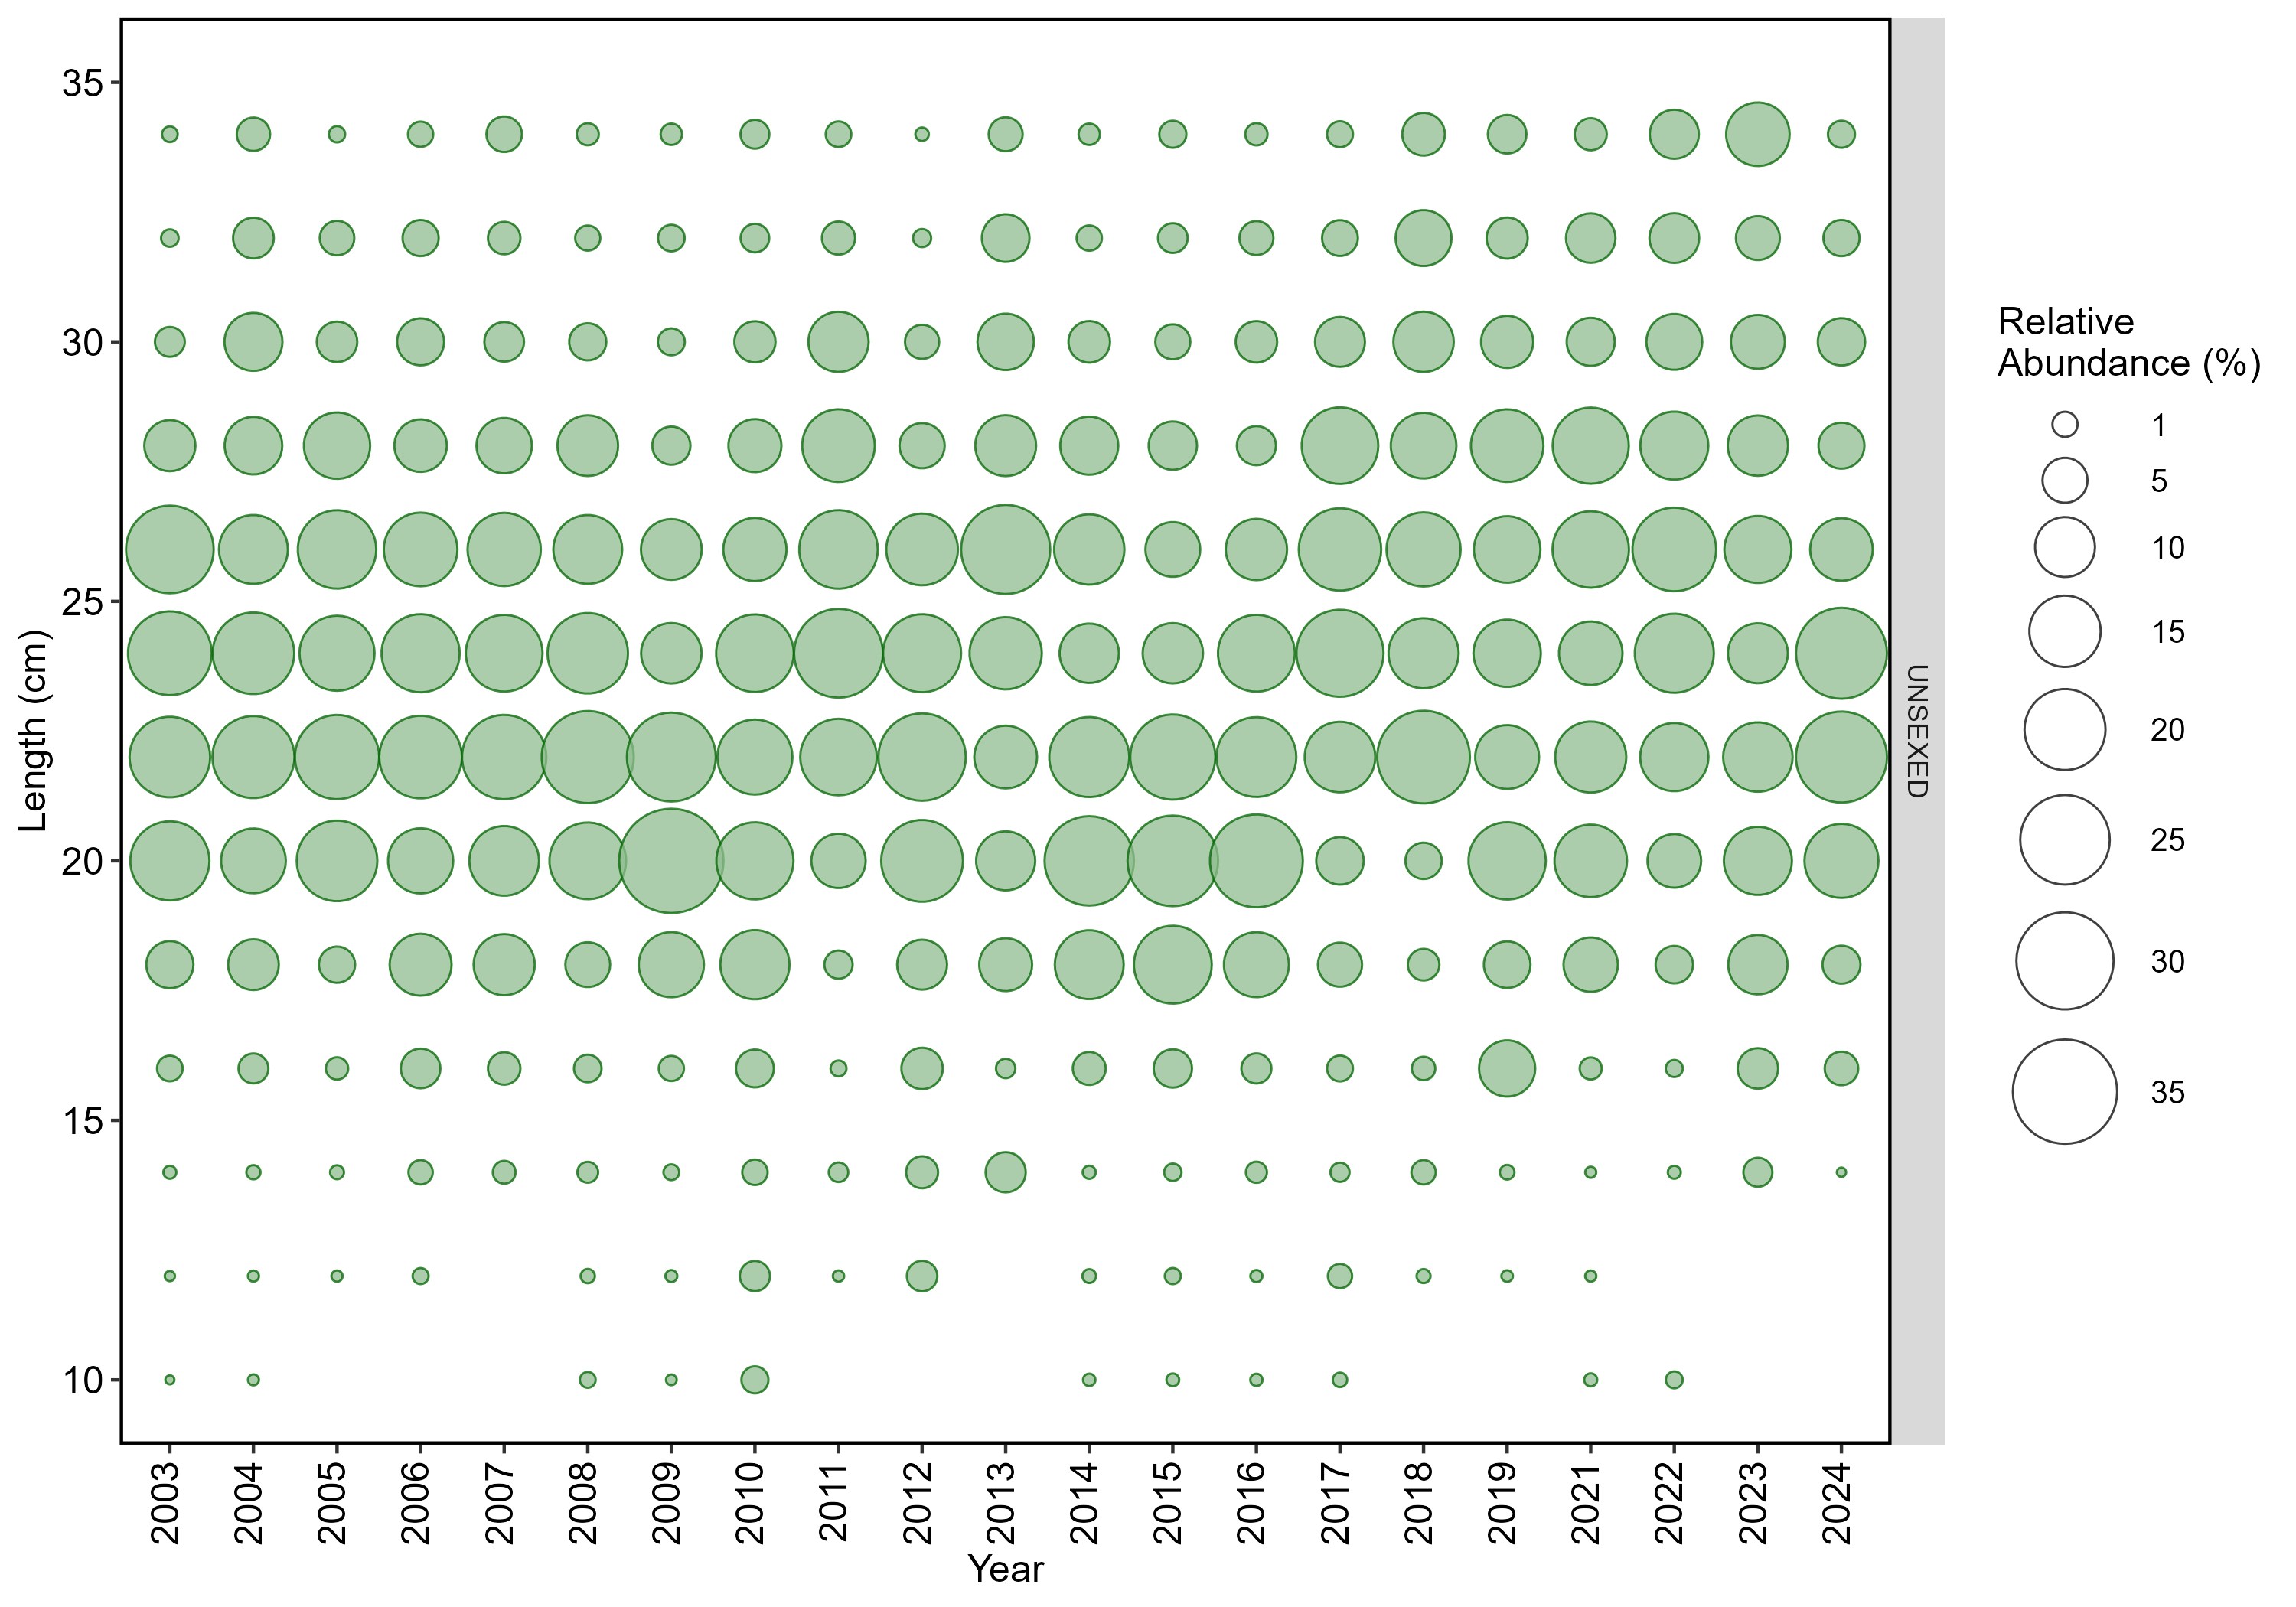
\includegraphics[width=0.95\linewidth,height=\textheight,keepaspectratio]{../plots/wcgbts_comps/plots/sharpchin rockfish_length_frequency_sex_0.png}

}

\caption{Length (cm) compostion data from the NWFSC WCGBTS for sharpchin
rockfish. Size of the circles within a year indicate higher (larger
circles) and lower (smaller circles) proportion observed by length bin.}

\end{figure}%

\newpage{}

\subsection{Shortspine thornyhead}\label{shortspine-thornyhead}

The most recent assessment of shortspine thornyhead was a data-moderate
assessment conducted in 2023. Across available data, shortspine
thornyhead have been observed and sampled by the NWFSC WCGBTS. The NWFSC
WCGBTS observed shortspine thornyhead on an average of 324 tows per
year. No validated (accurate and precise) aging methology currently
exists for shortspine thornyhead. For this species, a total of 1136
maturity samples have been collected coastwide (regardless of stock
area), with 862 read maturities.

\begingroup\fontsize{10}{12}\selectfont
\begingroup\fontsize{10}{12}\selectfont

\begin{longtable}[t]{>{\raggedleft\arraybackslash}p{2cm}>{\raggedleft\arraybackslash}p{3.5cm}>{\raggedleft\arraybackslash}p{2cm}>{\raggedleft\arraybackslash}p{2cm}>{\raggedleft\arraybackslash}p{2cm}}
\caption{\label{tab:unnamed-chunk-585}Total number of available lengths, read ages, and unread age structures by data source and
state for shortspine thornyhead.}\\
\toprule
State & Source & Lengths & Ages & Age Structures\\
\midrule
\endfirsthead
\caption[]{Total number of available lengths, read ages, and unread age structures by data source and
state for shortspine thornyhead. (\textit{continued)}}\\
\toprule
State & Source & Lengths & Ages & Age Structures\\
\midrule
\endhead

\endfoot
\bottomrule
\endlastfoot
CA & NWFSC WCGBTS & 50,554 & 0 & 12,492\\
OR & NWFSC WCGBTS & 44,504 & 0 & 7,554\\
WA & NWFSC WCGBTS & 12,983 & 0 & 2,789\\*
\end{longtable}
\endgroup{}
\endgroup{}

\begin{figure}[H]

{\centering 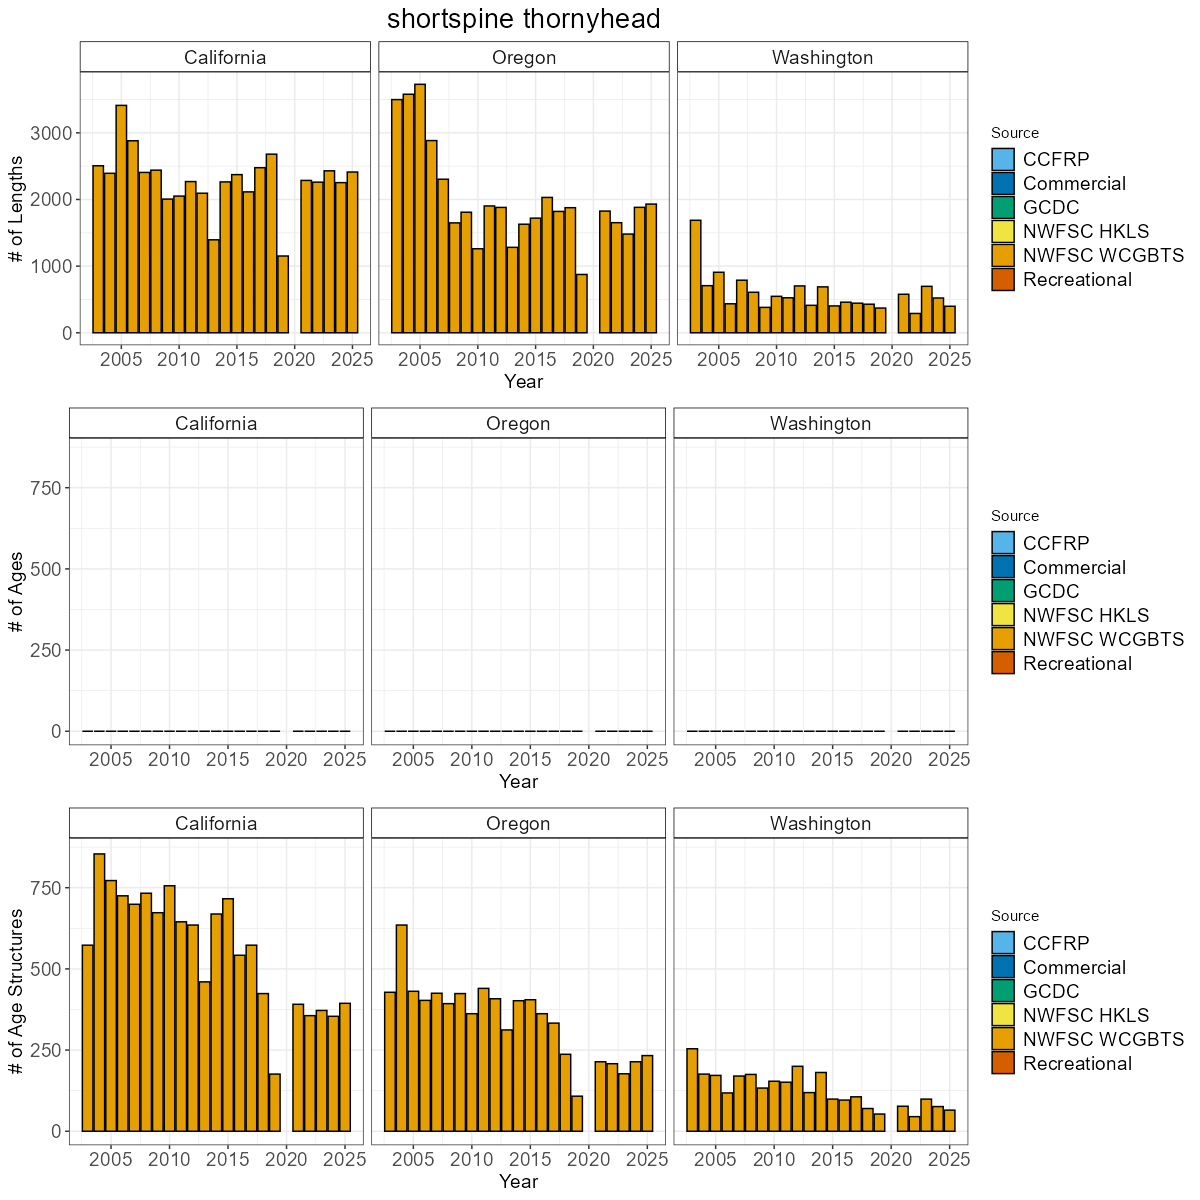
\includegraphics[width=0.95\linewidth,height=\textheight,keepaspectratio]{../plots/state_comparisons/shortspine_thornyhead_state_compositions.png}

}

\caption{Total number of available lengths, read ages, and unread age
structures by data source by year for shortspine thornyhead. Note the
y-axis maximum may differ by data type.}

\end{figure}%

\begin{figure}[H]

{\centering 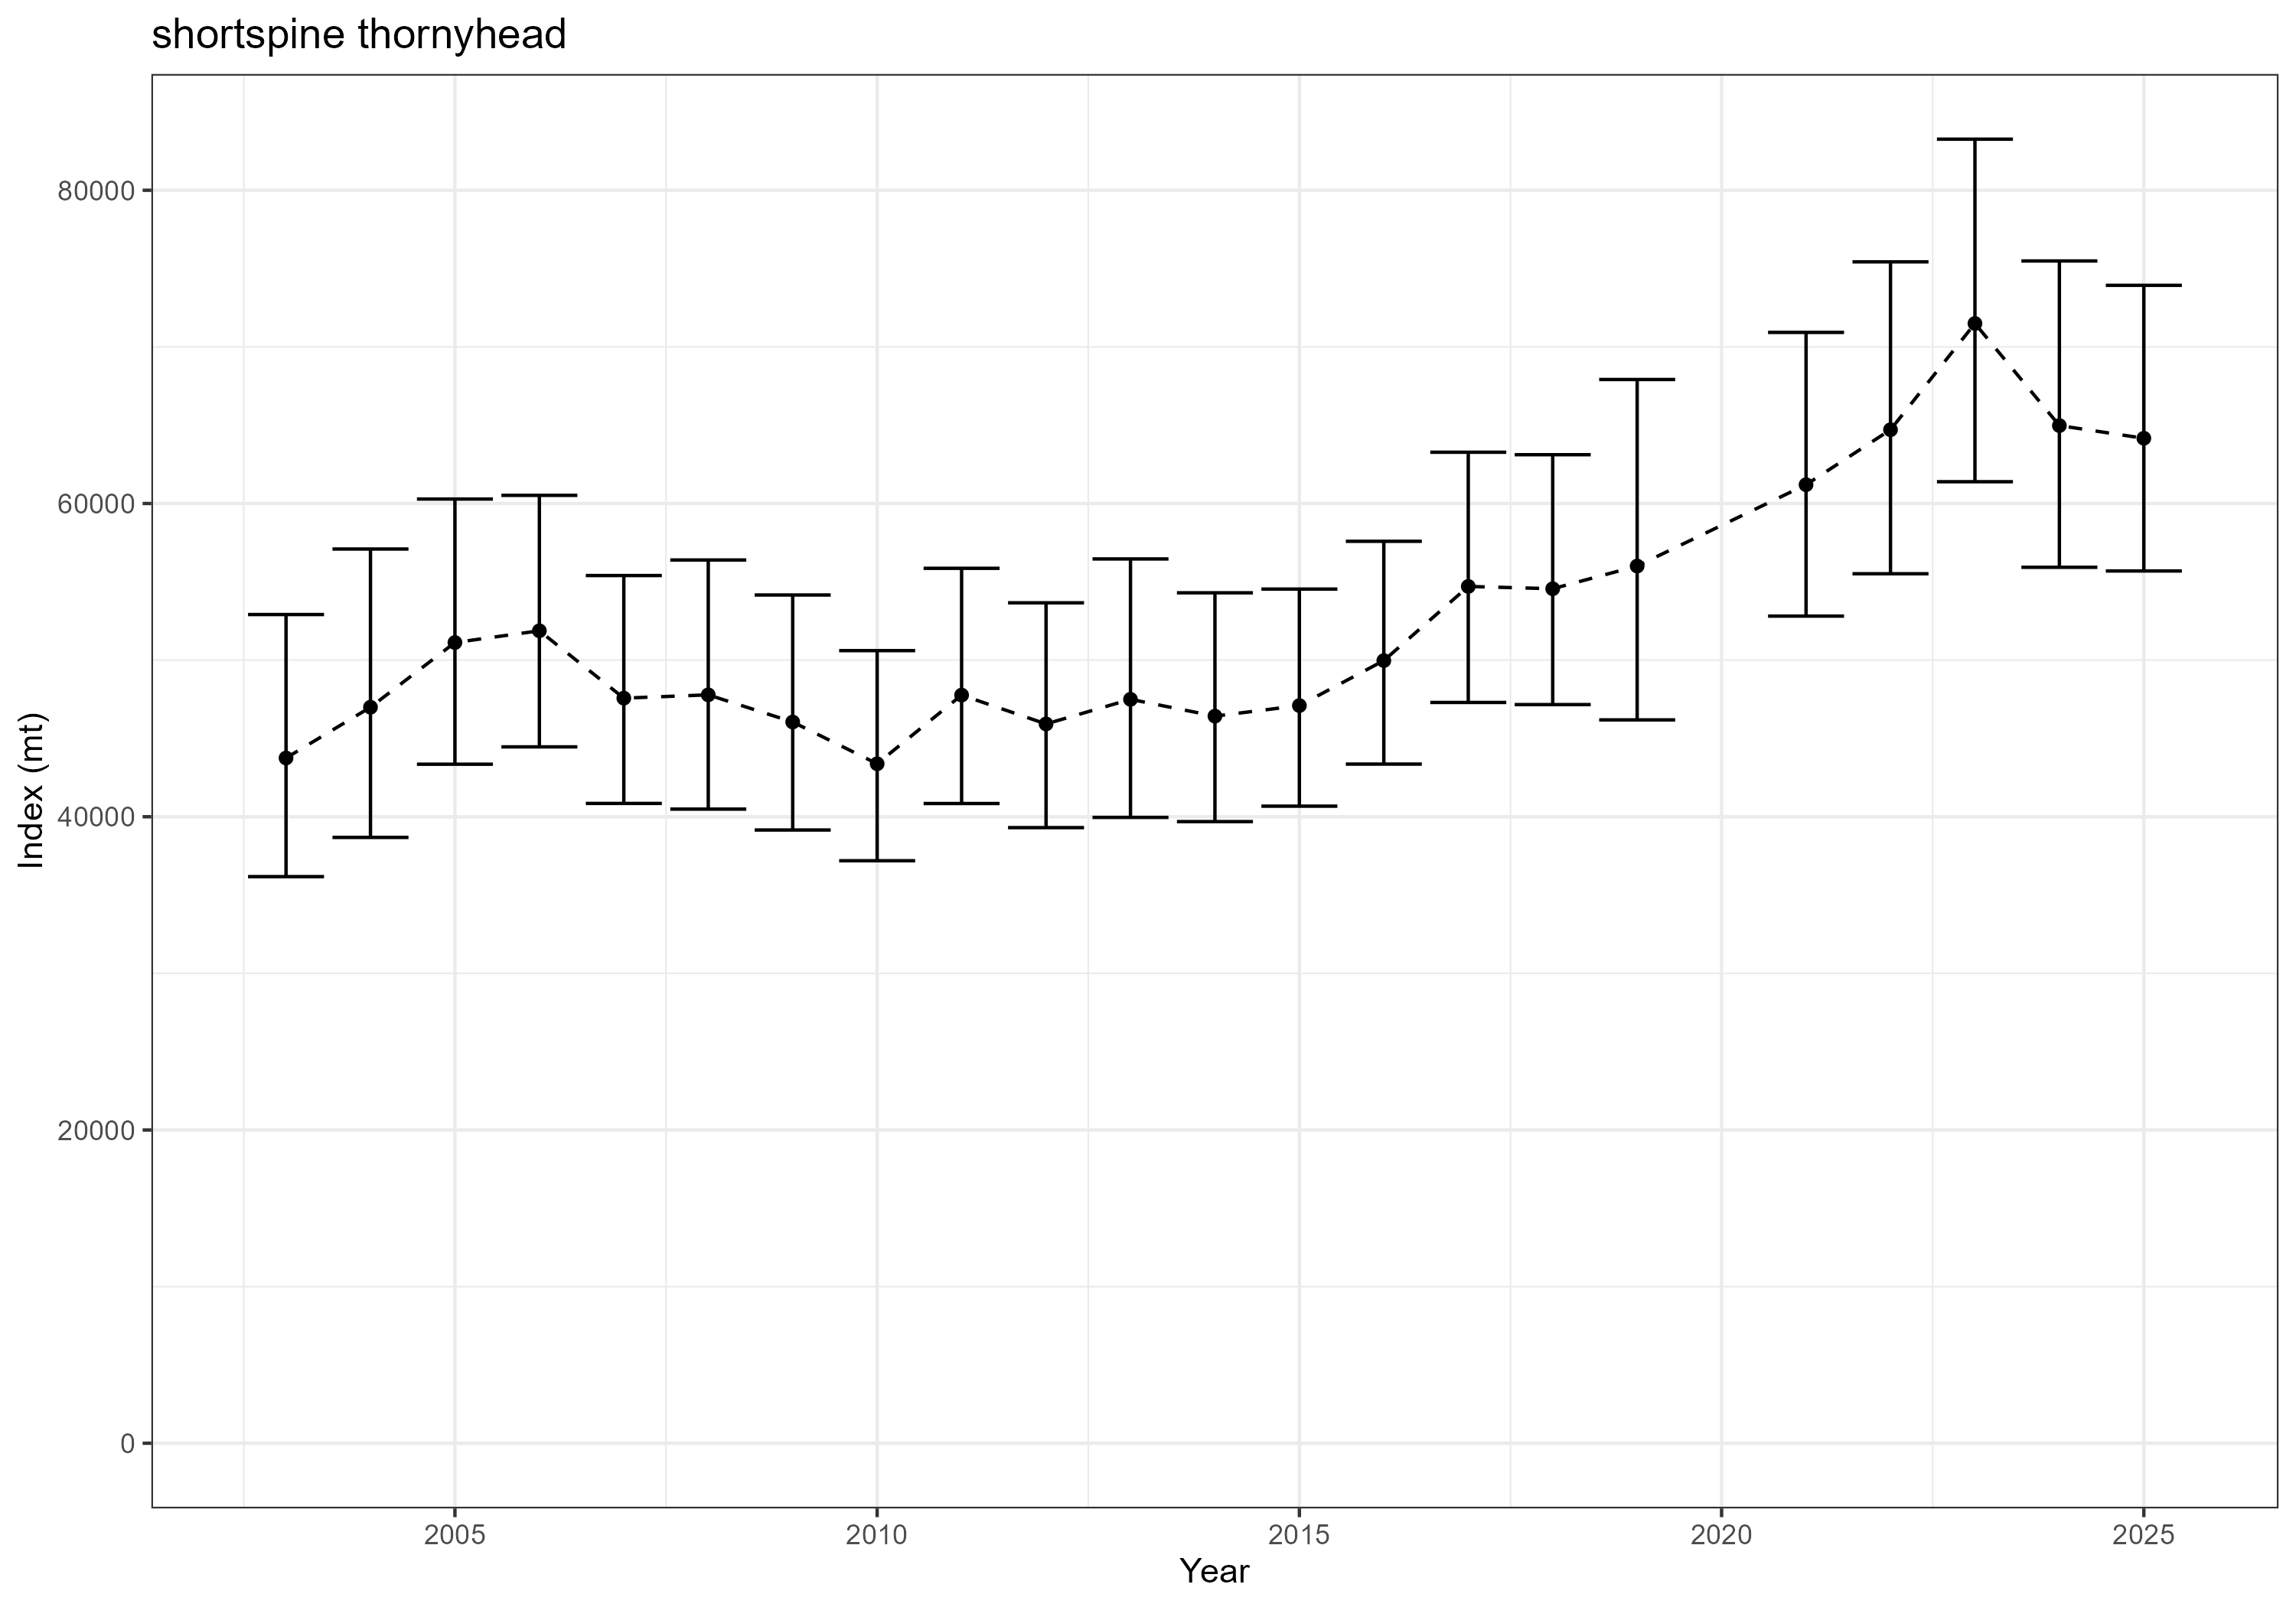
\includegraphics[width=0.95\linewidth,height=\textheight,keepaspectratio]{../plots/additional_wcgbts_indices/shortspine_thornyhead_index.png}

}

\caption{Estimated relative index of abundance for shortspine thornyhead
from the NWFSC WCGBTS.}

\end{figure}%

\begin{figure}[H]

{\centering 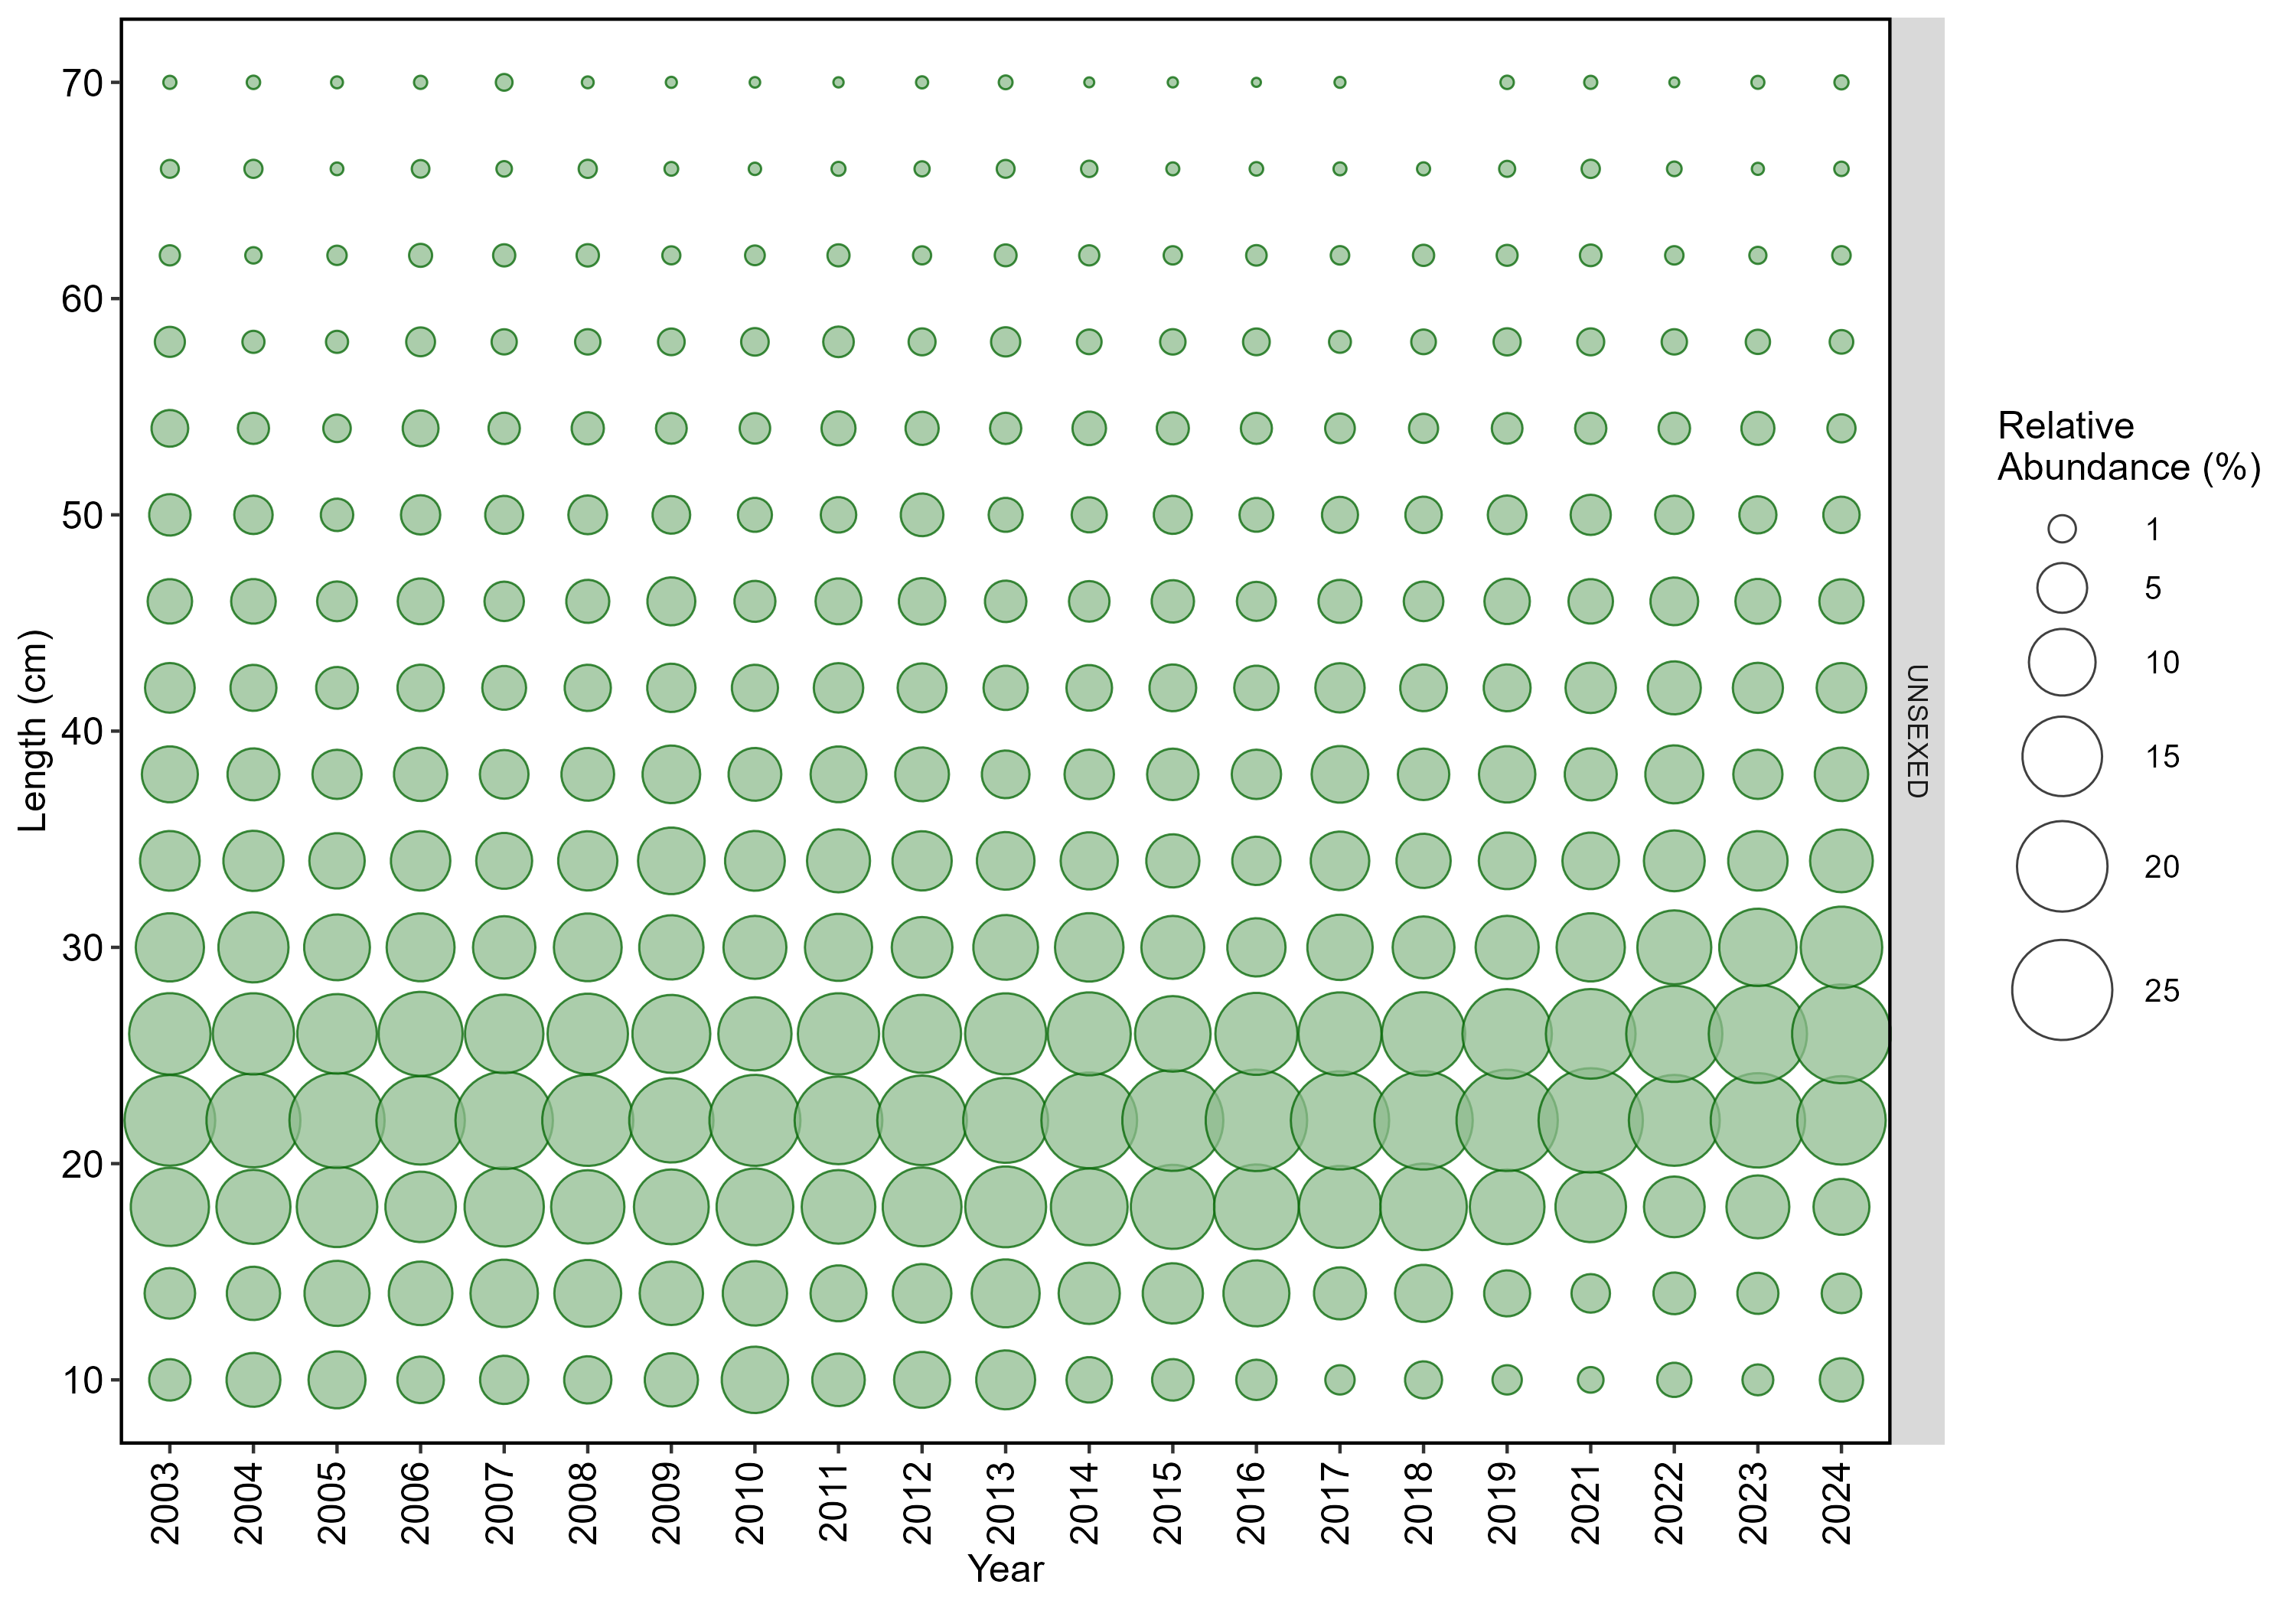
\includegraphics[width=0.95\linewidth,height=\textheight,keepaspectratio]{../plots/wcgbts_comps/plots/shortspine thornyhead_length_frequency_sex_0.png}

}

\caption{Length (cm) compostion data from the NWFSC WCGBTS for
shortspine thornyhead. Size of the circles within a year indicate higher
(larger circles) and lower (smaller circles) proportion observed by
length bin.}

\end{figure}%

\newpage{}

\subsection{Silvergray rockfish}\label{silvergray-rockfish}

To date, no assessment or analysis has been conducted on silvergray
rockfish. Across available data, silvergray rockfish have been observed
and sampled by both the NWFSC HKLS and WCGBTS. The NWFSC HKLS observed
silvergray rockfish at an average of 0 sets per year. The NWFSC WCGBTS
observed silvergray rockfish on an average of 6 tows per year. For this
species, a total of 0 maturity samples have been collected coastwide
(regardless of stock area).

\begingroup\fontsize{10}{12}\selectfont
\begingroup\fontsize{10}{12}\selectfont

\begin{longtable}[t]{>{\raggedleft\arraybackslash}p{2cm}>{\raggedleft\arraybackslash}p{3.5cm}>{\raggedleft\arraybackslash}p{2cm}>{\raggedleft\arraybackslash}p{2cm}>{\raggedleft\arraybackslash}p{2cm}}
\caption{\label{tab:unnamed-chunk-602}Total number of available lengths, read ages, and unread age structures by data source and
state for silvergray rockfish.}\\
\toprule
State & Source & Lengths & Ages & Age Structures\\
\midrule
\endfirsthead
\caption[]{Total number of available lengths, read ages, and unread age structures by data source and
state for silvergray rockfish. (\textit{continued)}}\\
\toprule
State & Source & Lengths & Ages & Age Structures\\
\midrule
\endhead

\endfoot
\bottomrule
\endlastfoot
CA & NWFSC HKLS & 4 & 0 & 3\\
CA & NWFSC WCGBTS & 16 & 0 & 16\\
OR & NWFSC WCGBTS & 492 & 0 & 404\\
WA & NWFSC WCGBTS & 455 & 0 & 428\\*
\end{longtable}
\endgroup{}
\endgroup{}

\begin{figure}[H]

{\centering 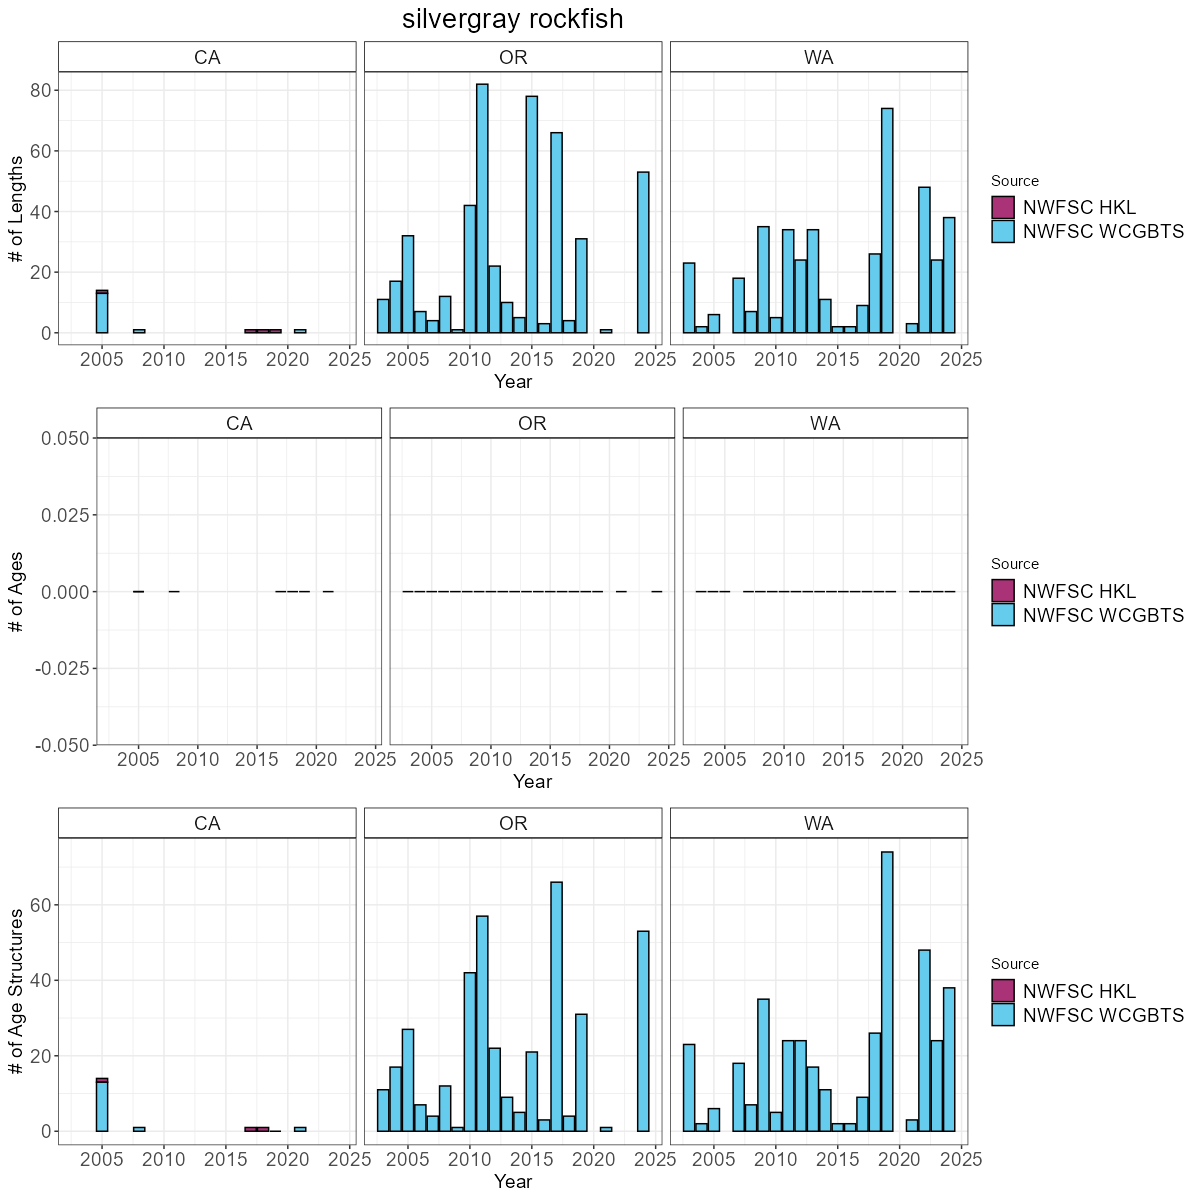
\includegraphics[width=0.95\linewidth,height=\textheight,keepaspectratio]{../plots/state_comparisons/silvergray_rockfish_state_compositions.png}

}

\caption{Total number of available lengths, read ages, and unread age
structures by data source by year for silvergray rockfish. Note the
y-axis maximum may differ by data type.}

\end{figure}%

\newpage{}

\subsection{Splitnose rockfish}\label{splitnose-rockfish}

The most recent assessment of splitnose rockfish was a benchmark
assessment conducted in 2009. Across available data, splitnose rockfish
have been observed and sampled by the NWFSC WCGBTS. The NWFSC WCGBTS
observed splitnose rockfish on an average of 128 tows per year. For this
species, a total of 0 maturity samples have been collected coastwide
(regardless of stock area).

\begingroup\fontsize{10}{12}\selectfont
\begingroup\fontsize{10}{12}\selectfont

\begin{longtable}[t]{>{\raggedleft\arraybackslash}p{2cm}>{\raggedleft\arraybackslash}p{3.5cm}>{\raggedleft\arraybackslash}p{2cm}>{\raggedleft\arraybackslash}p{2cm}>{\raggedleft\arraybackslash}p{2cm}}
\caption{\label{tab:unnamed-chunk-619}Total number of available lengths, read ages, and unread age structures by data source and
state for splitnose rockfish.}\\
\toprule
State & Source & Lengths & Ages & Age Structures\\
\midrule
\endfirsthead
\caption[]{Total number of available lengths, read ages, and unread age structures by data source and
state for splitnose rockfish. (\textit{continued)}}\\
\toprule
State & Source & Lengths & Ages & Age Structures\\
\midrule
\endhead

\endfoot
\bottomrule
\endlastfoot
CA & NWFSC WCGBTS & 34,562 & 1,573 & 6,339\\
OR & NWFSC WCGBTS & 18,617 & 1,044 & 3,776\\
WA & NWFSC WCGBTS & 3,185 & 294 & 668\\*
\end{longtable}
\endgroup{}
\endgroup{}

\begin{figure}[H]

{\centering 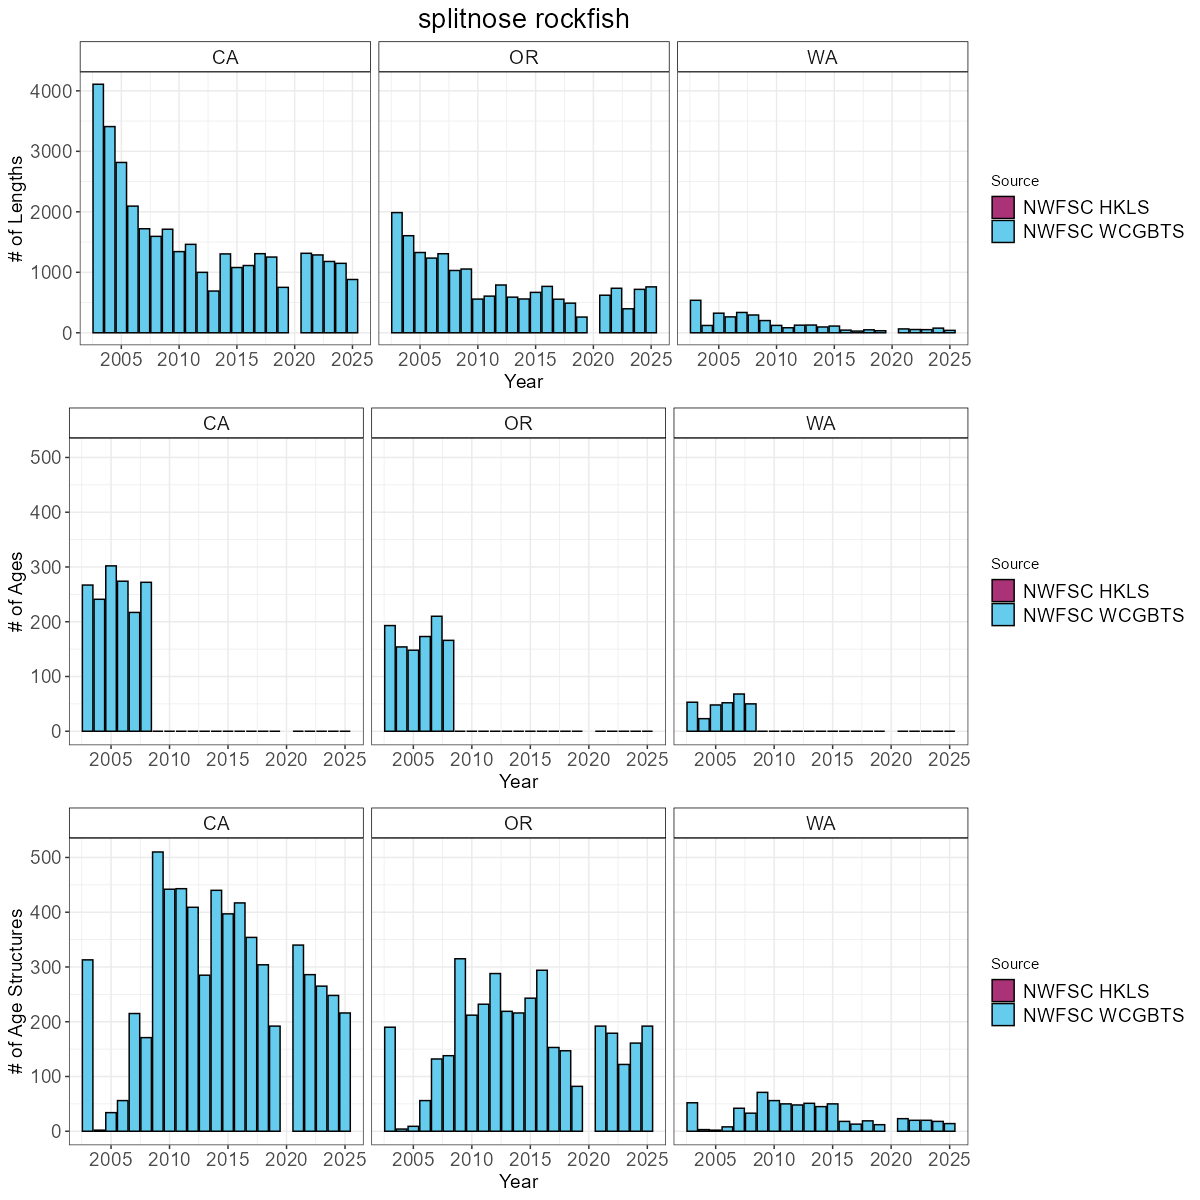
\includegraphics[width=0.95\linewidth,height=\textheight,keepaspectratio]{../plots/state_comparisons/splitnose_rockfish_state_compositions.png}

}

\caption{Total number of available lengths, read ages, and unread age
structures by data source by year for splitnose rockfish. Note the
y-axis maximum may differ by data type.}

\end{figure}%

\begin{figure}[H]

{\centering 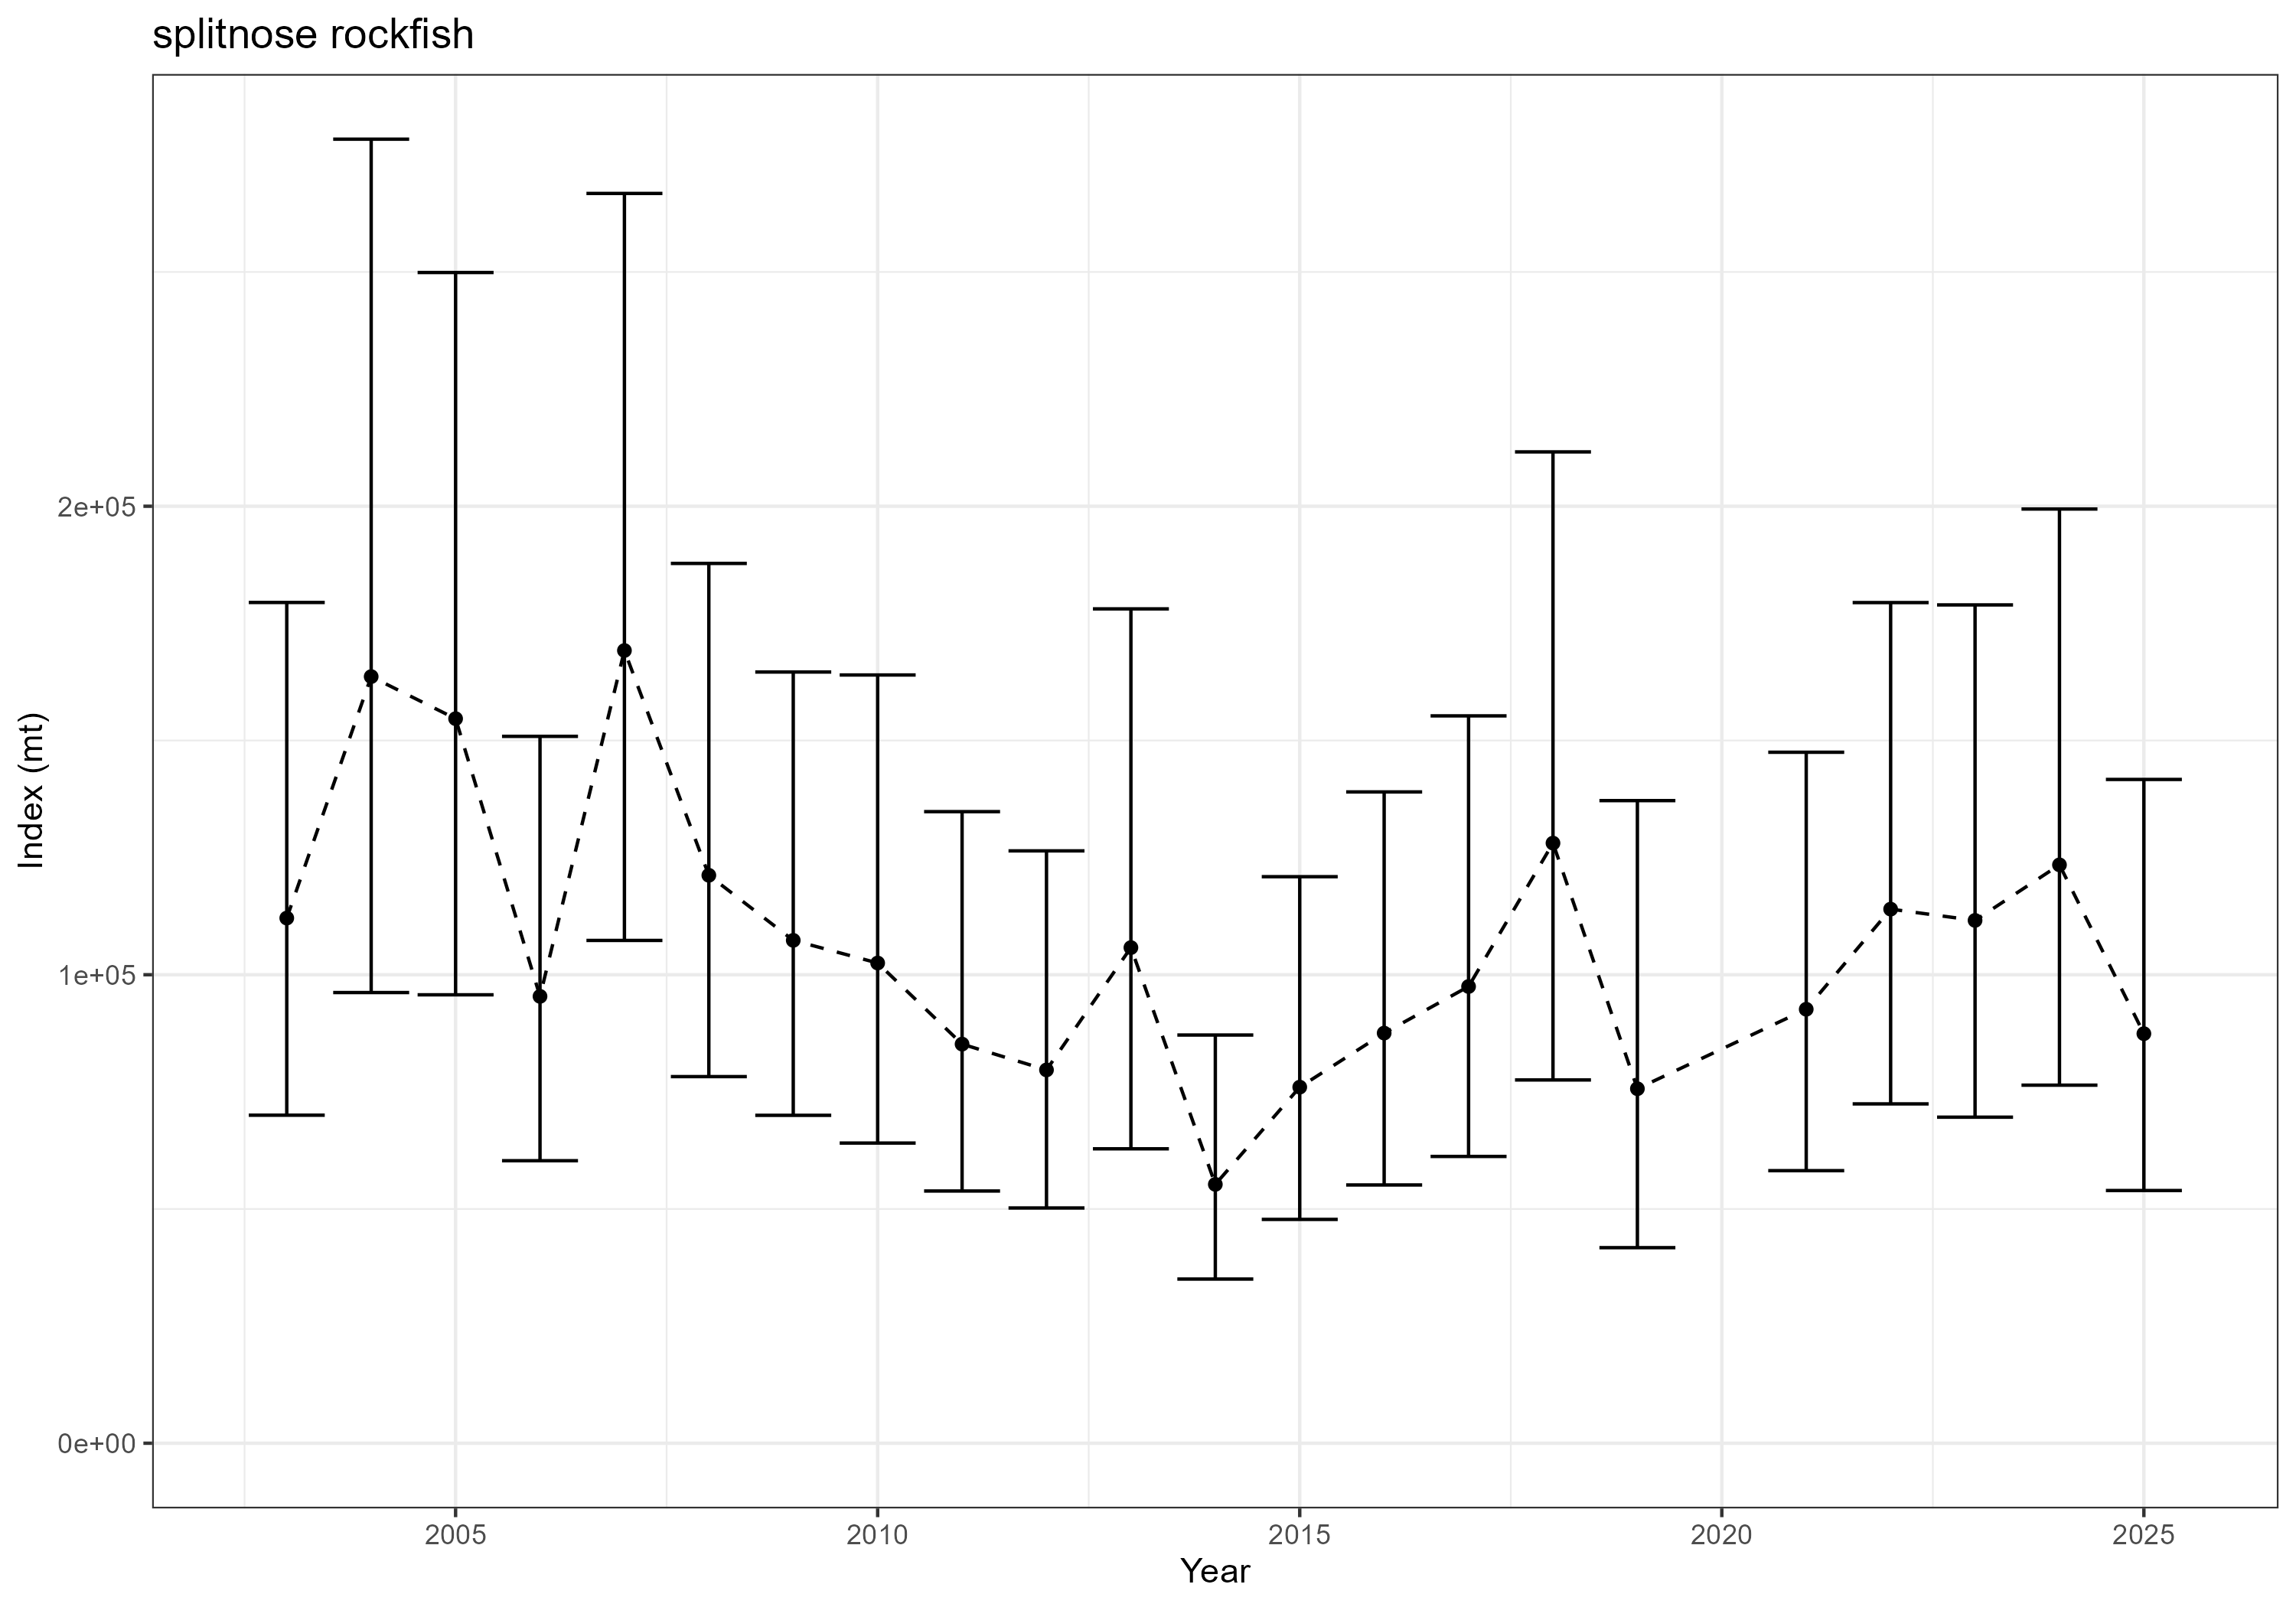
\includegraphics[width=0.95\linewidth,height=\textheight,keepaspectratio]{../plots/wcgbts_indices/splitnose_rockfish_index.png}

}

\caption{Estimated relative index of abundance for splitnose rockfish
from the NWFSC WCGBTS.}

\end{figure}%

\begin{figure}[H]

{\centering 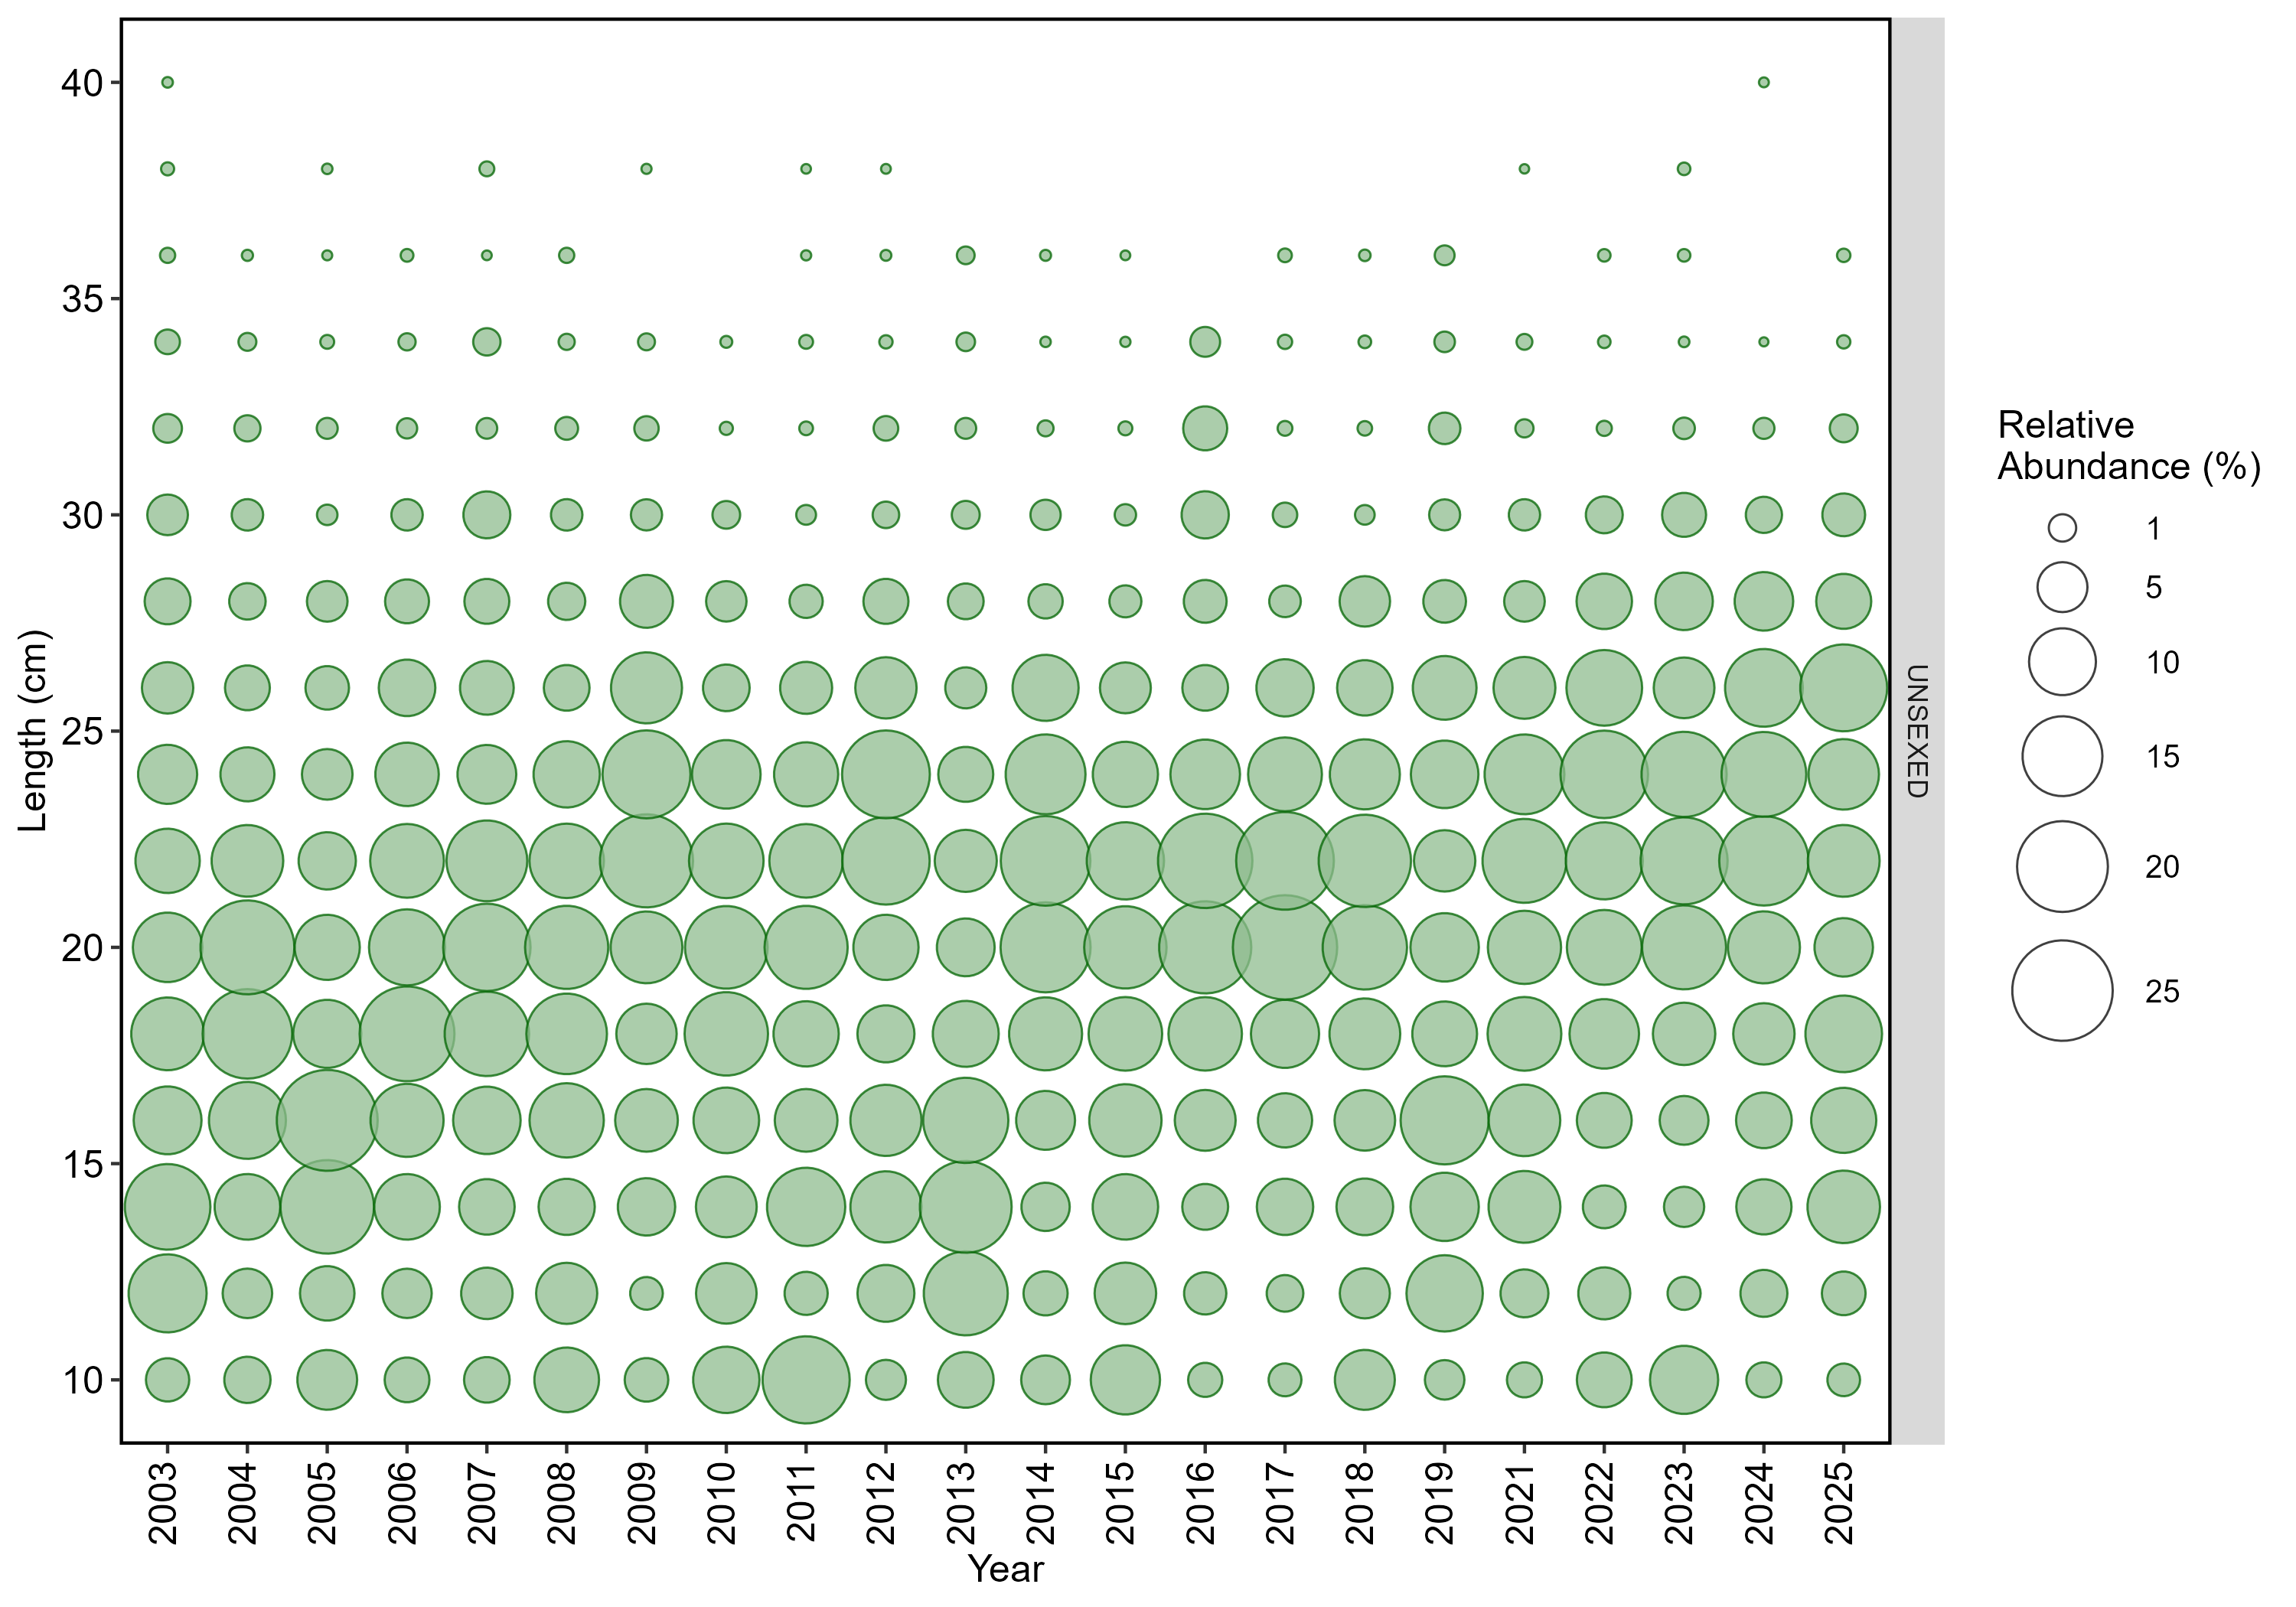
\includegraphics[width=0.95\linewidth,height=\textheight,keepaspectratio]{../plots/wcgbts_comps/plots/splitnose rockfish_length_frequency_sex_0.png}

}

\caption{Length (cm) compostion data from the NWFSC WCGBTS for splitnose
rockfish. Size of the circles within a year indicate higher (larger
circles) and lower (smaller circles) proportion observed by length bin.}

\end{figure}%

\newpage{}

\subsection{Squarespot rockfish}\label{squarespot-rockfish}

The most recent assessment of squarespot rockfish was a data-moderate
assessment conducted in 2021. Across available data, squarespot rockfish
have been observed and sampled by both the NWFSC HKLS and WCGBTS. The
NWFSC HKLS observed squarespot rockfish at an average of 32 sets per
year. The NWFSC WCGBTS observed squarespot rockfish on an average of 10
tows per year. For this species, a total of 118 maturity samples have
been collected coastwide (regardless of stock area), with 118 read
maturities.

\begingroup\fontsize{10}{12}\selectfont
\begingroup\fontsize{10}{12}\selectfont

\begin{longtable}[t]{>{\raggedleft\arraybackslash}p{2cm}>{\raggedleft\arraybackslash}p{3.5cm}>{\raggedleft\arraybackslash}p{2cm}>{\raggedleft\arraybackslash}p{2cm}>{\raggedleft\arraybackslash}p{2cm}}
\caption{\label{tab:unnamed-chunk-636}Total number of available lengths, read ages, and unread age structures by data source and
state for squarespot rockfish.}\\
\toprule
State & Source & Lengths & Ages & Age Structures\\
\midrule
\endfirsthead
\caption[]{Total number of available lengths, read ages, and unread age structures by data source and
state for squarespot rockfish. (\textit{continued)}}\\
\toprule
State & Source & Lengths & Ages & Age Structures\\
\midrule
\endhead

\endfoot
\bottomrule
\endlastfoot
CA & NWFSC HKLS & 2,618 & 344 & 2,170\\
CA & NWFSC WCGBTS & 5,031 & 402 & 1,302\\
OR & NWFSC WCGBTS & 4 & 1 & 1\\*
\end{longtable}
\endgroup{}
\endgroup{}

\begin{figure}[H]

{\centering 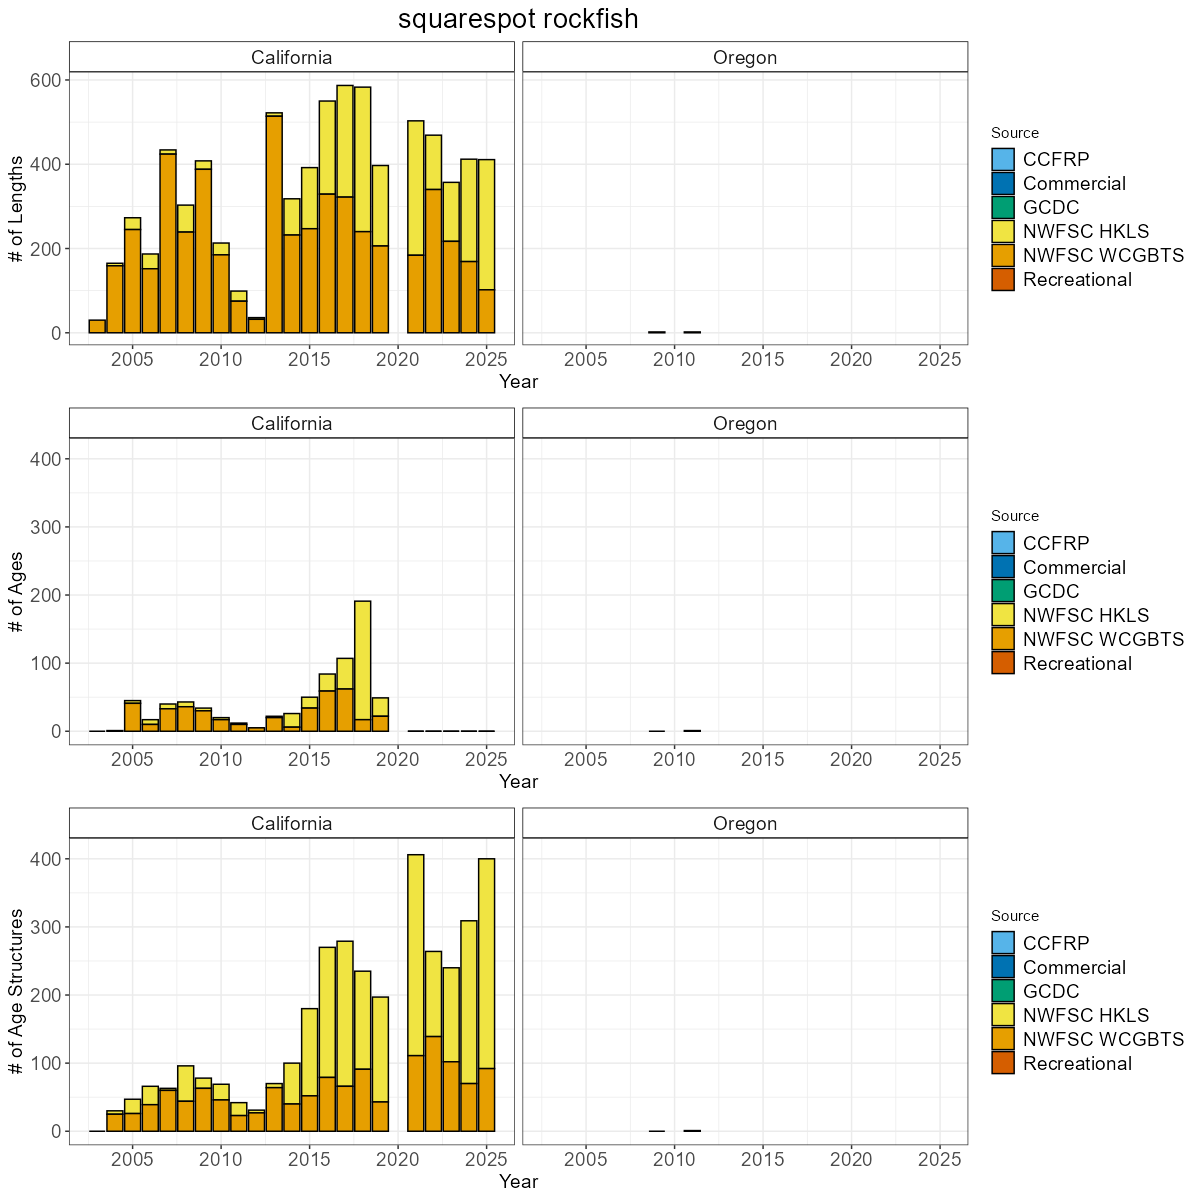
\includegraphics[width=0.95\linewidth,height=\textheight,keepaspectratio]{../plots/state_comparisons/squarespot_rockfish_state_compositions.png}

}

\caption{Total number of available lengths, read ages, and unread age
structures by data source by year for squarespot rockfish. Note the
y-axis maximum may differ by data type.}

\end{figure}%

\begin{figure}[H]

{\centering 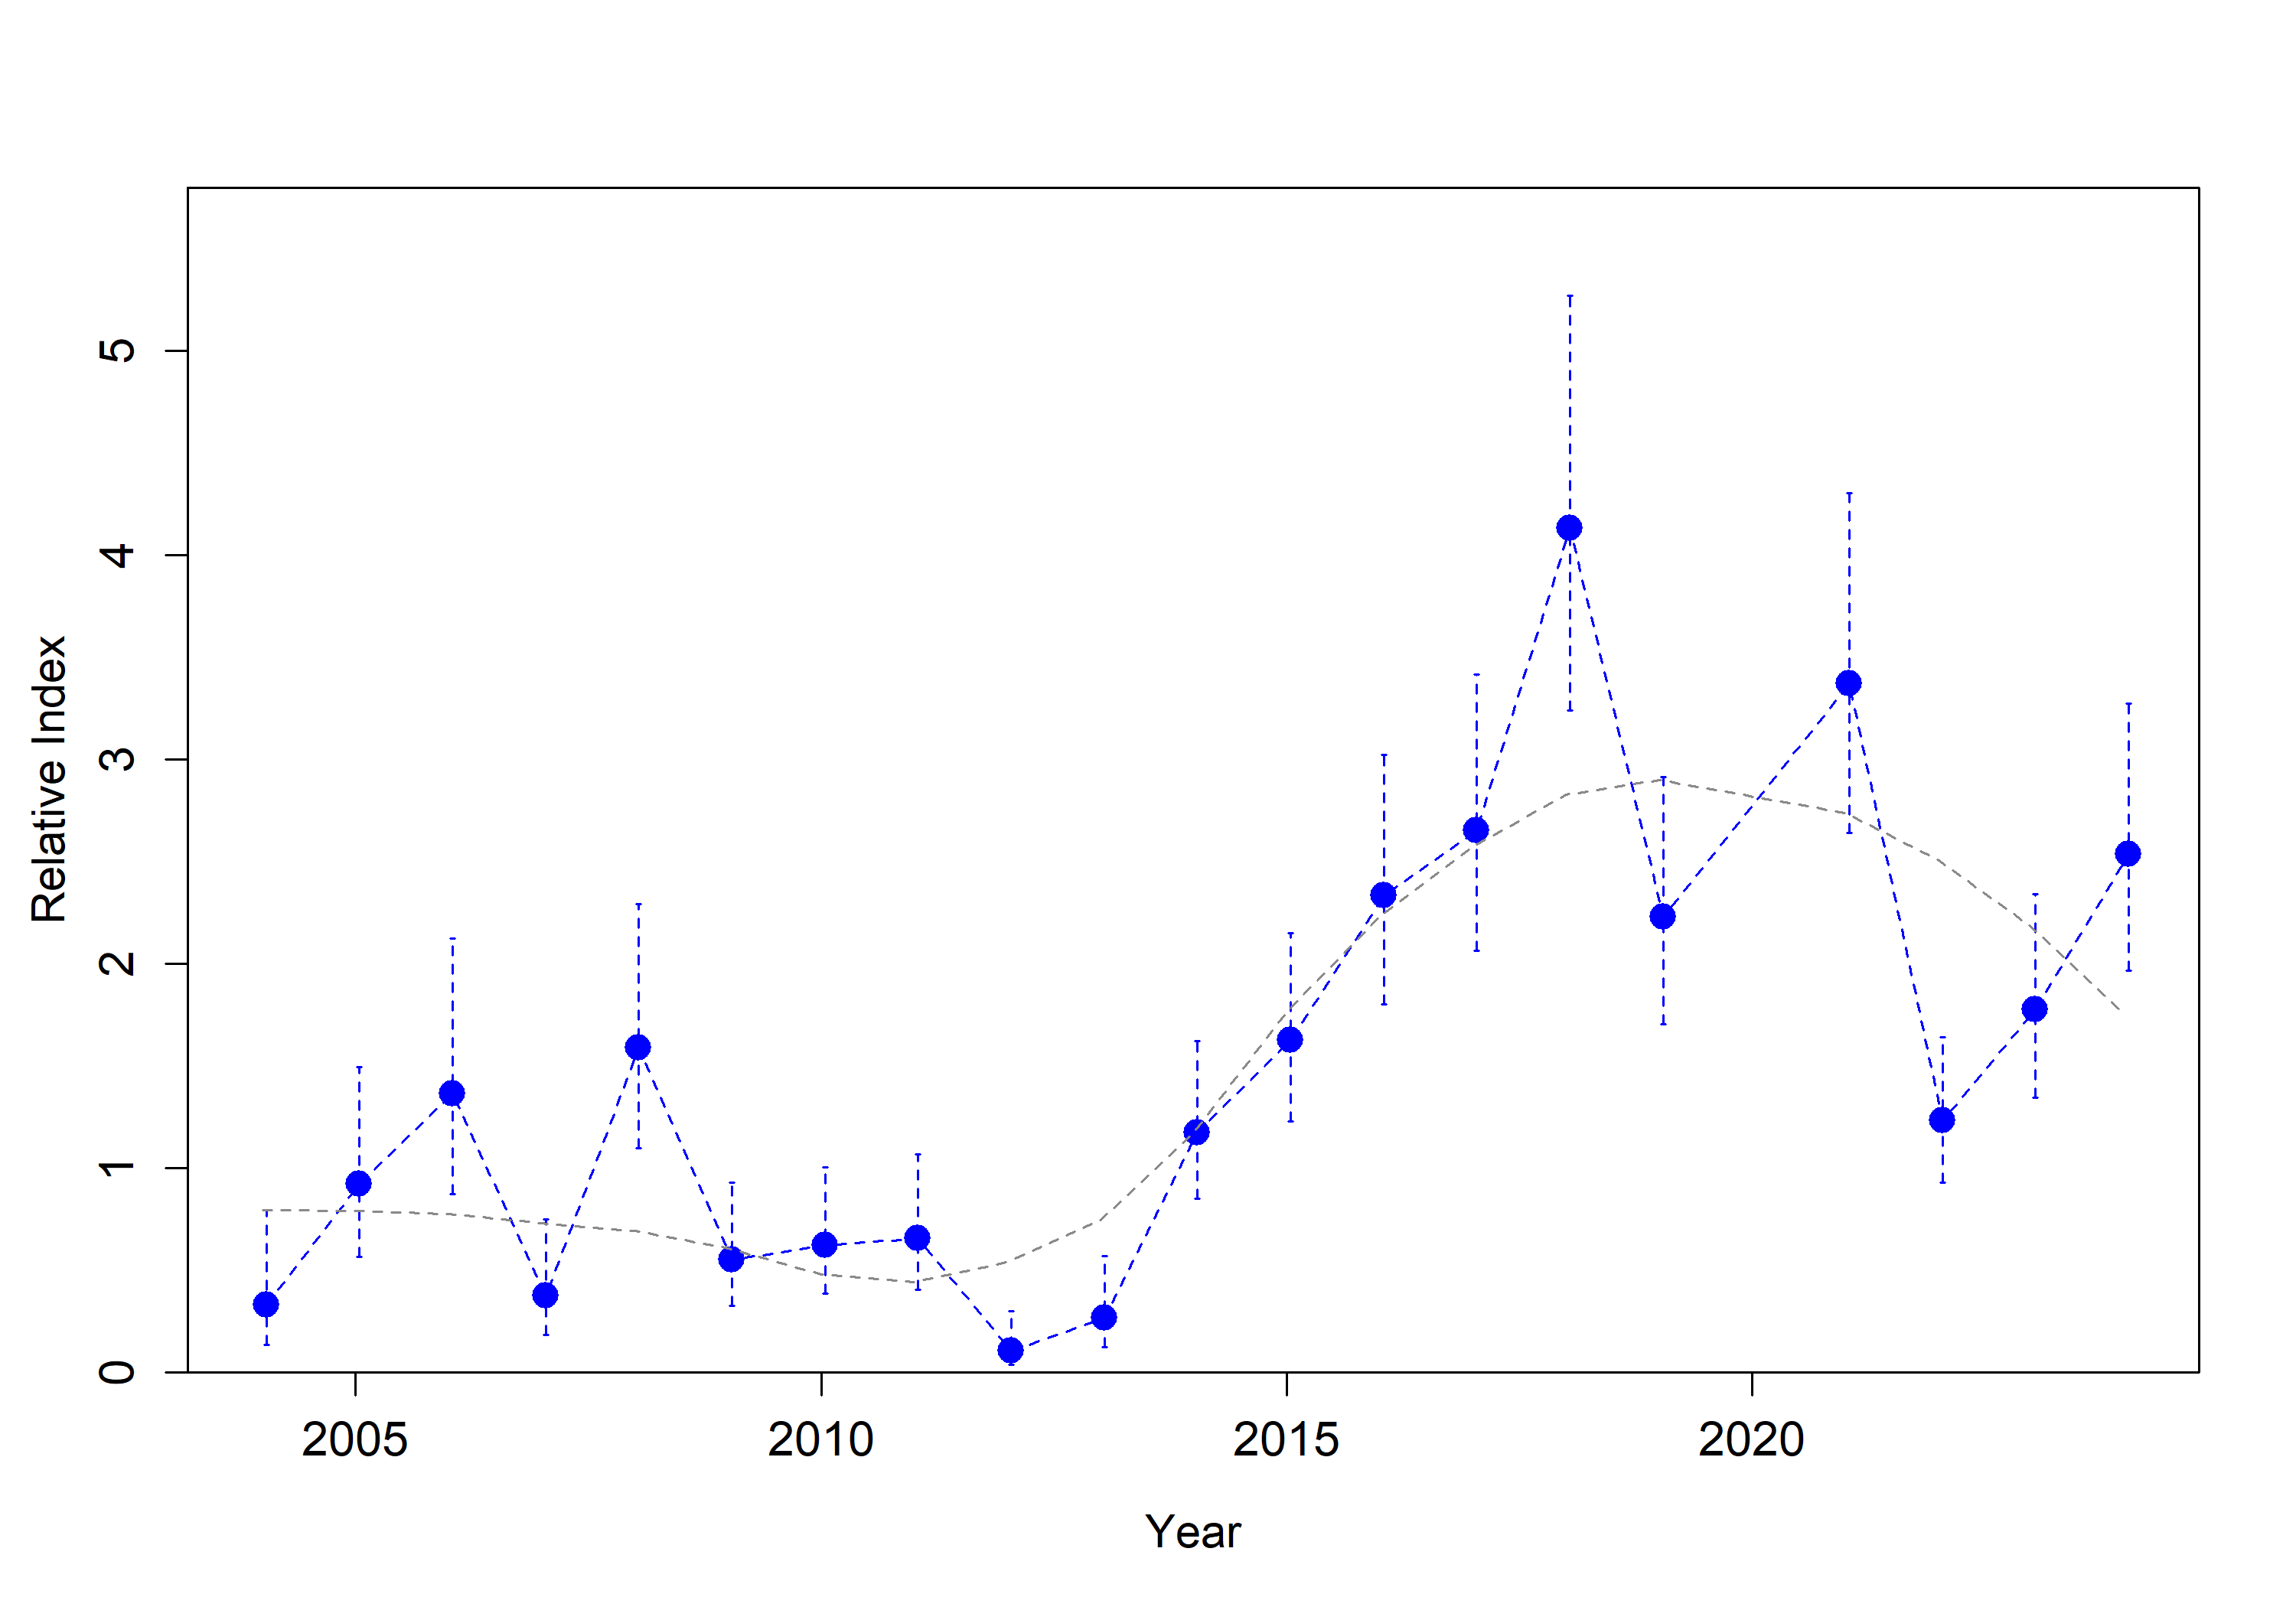
\includegraphics[width=0.95\linewidth,height=\textheight,keepaspectratio]{../plots/hkl_indices/squarespot rockfish_negbinom index.png}

}

\caption{Estimated relative index of abundance for squarespot rockfish
from the NWFSC HKLS.}

\end{figure}%

\begin{figure}[H]

{\centering 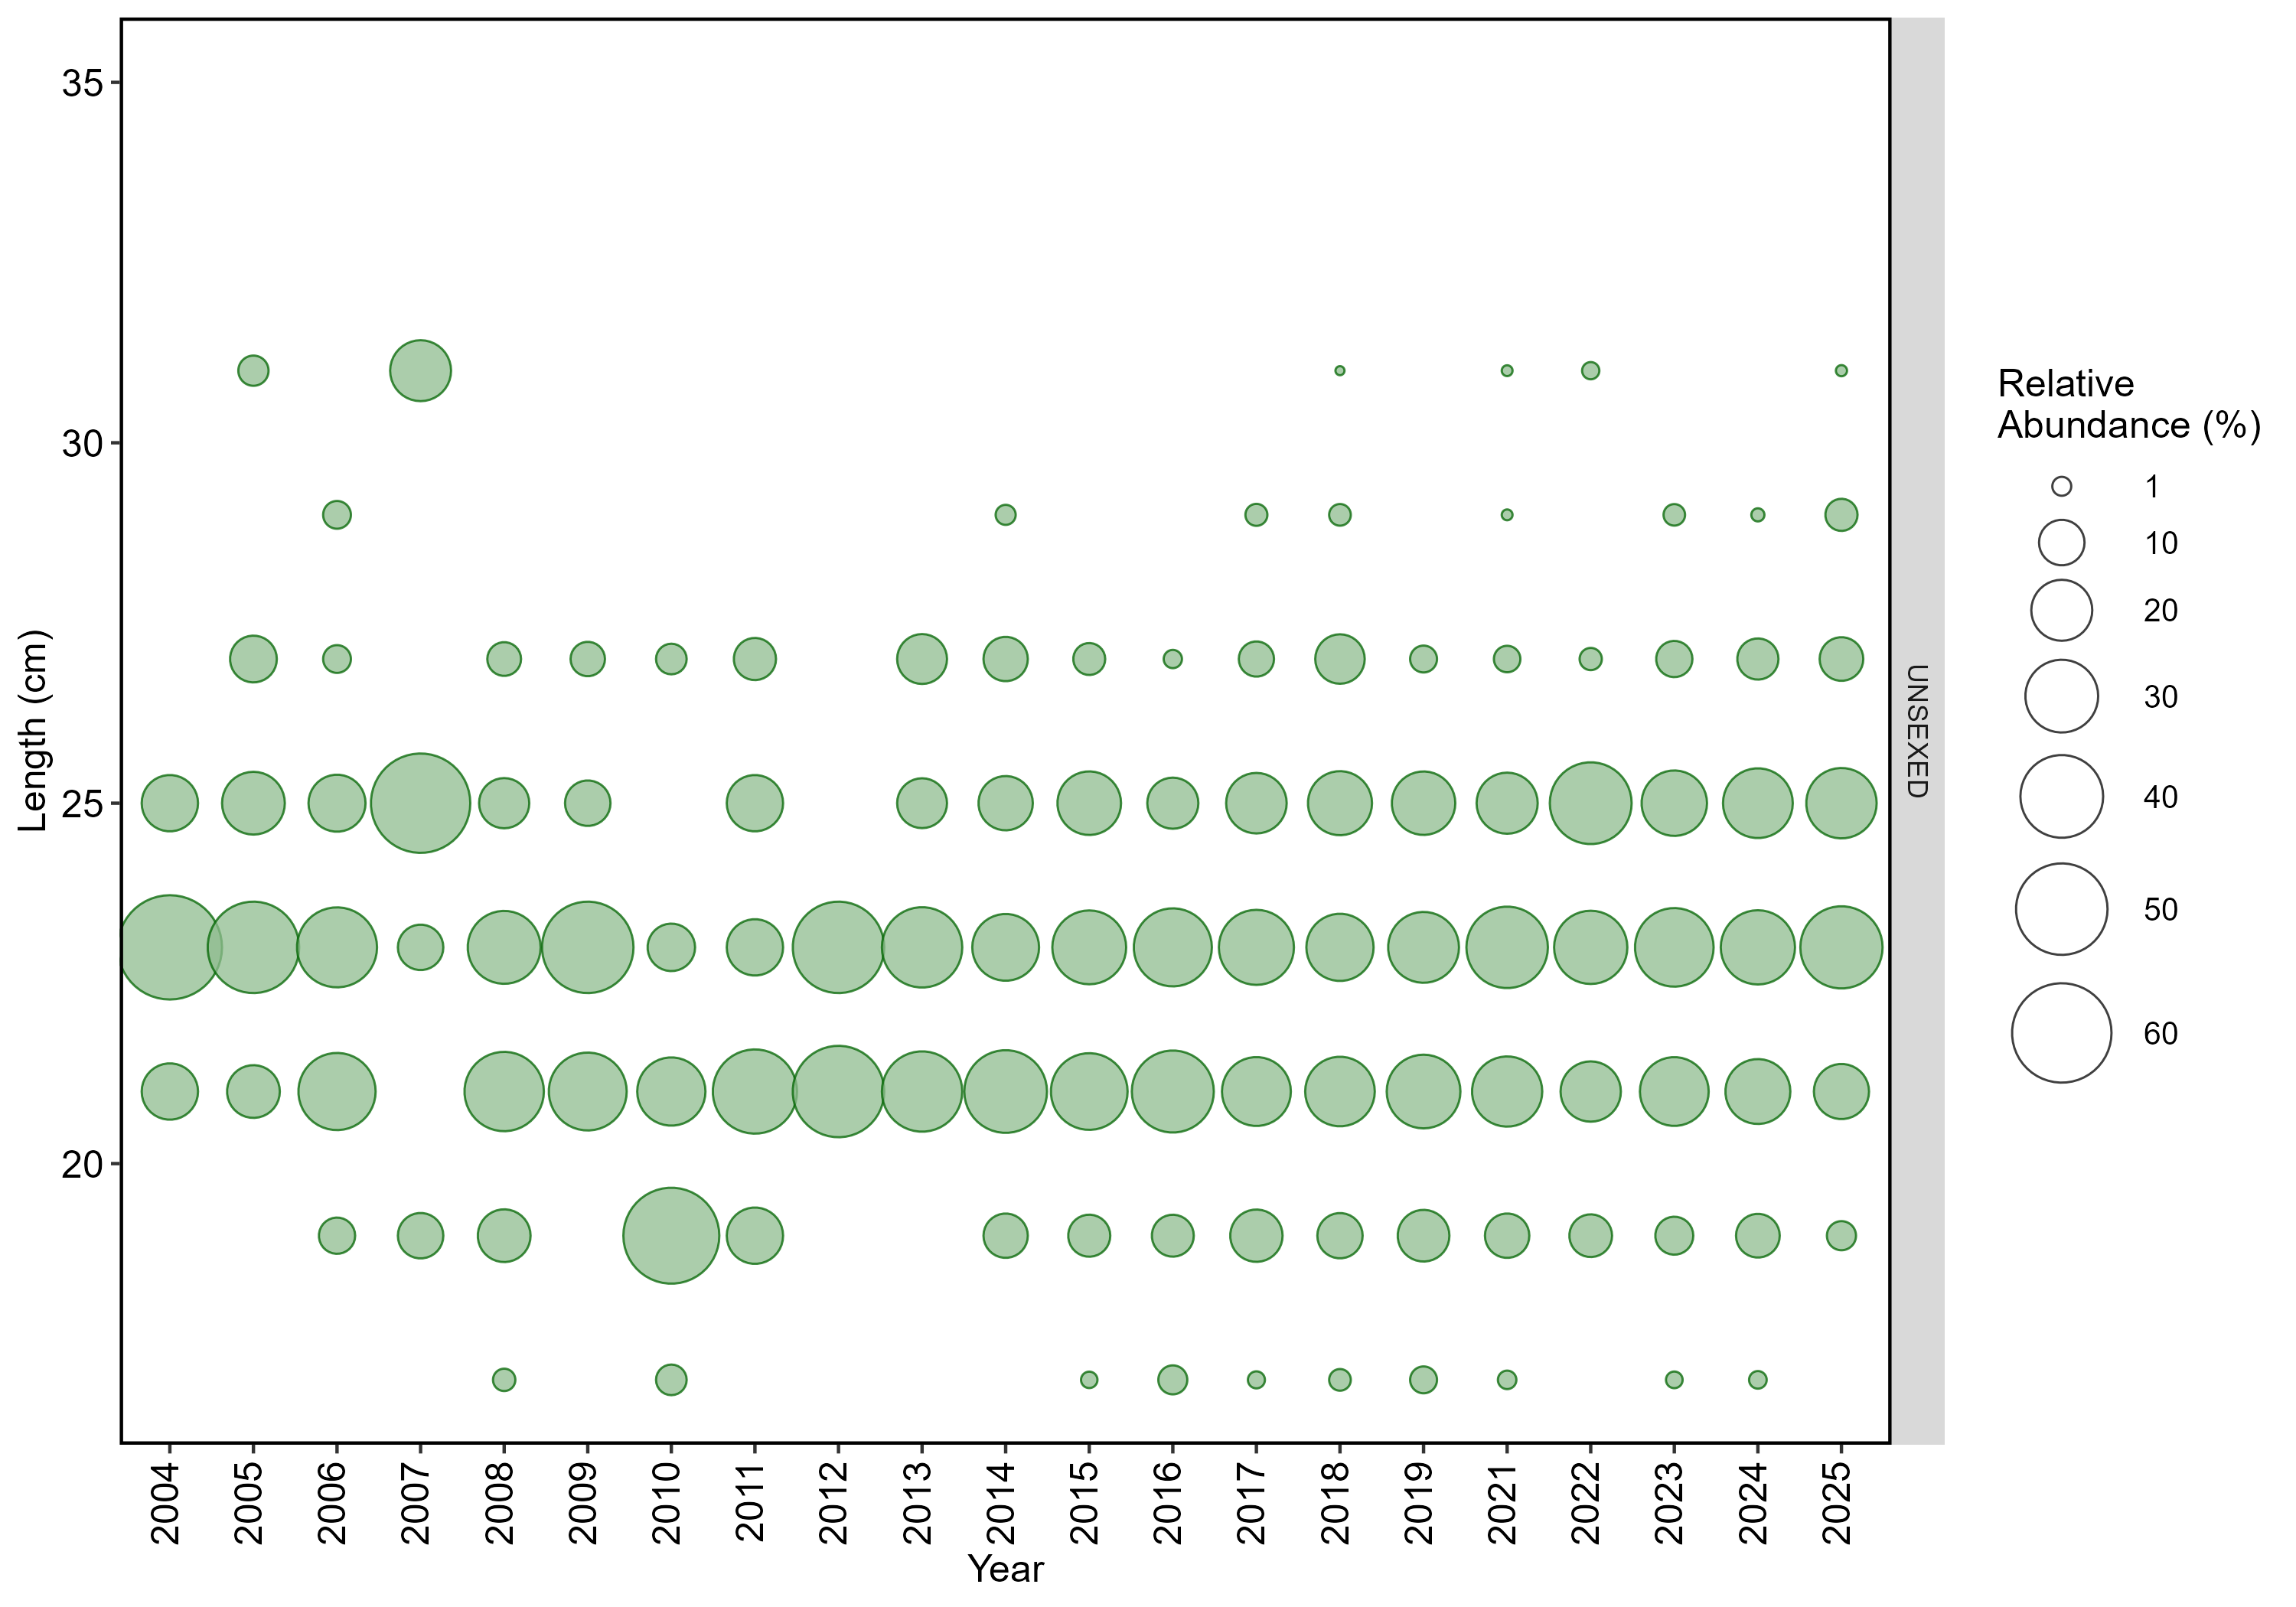
\includegraphics[width=0.95\linewidth,height=\textheight,keepaspectratio]{../plots/additional_hkl_comps/plots/squarespot rockfish_nwfsc_hkl_length_frequency_sex_0.png}

}

\caption{Length (cm) compostion data from the NWFSC HKLS for squarespot
rockfish. Size of the circles within a year indicate higher (larger
circles) and lower (smaller circles) proportion observed by length bin.}

\end{figure}%

\newpage{}

\subsection{Starry rockfish}\label{starry-rockfish}

To date, no assessment or analysis has been conducted on starry
rockfish. Across available data, starry rockfish have been observed and
sampled by both the NWFSC HKLS and WCGBTS. The NWFSC HKLS observed
starry rockfish at an average of 57 sets per year. The NWFSC WCGBTS
observed starry rockfish on an average of 2 tows per year. For this
species, a total of 340 maturity samples have been collected coastwide
(regardless of stock area), with 0 read maturities.

\begingroup\fontsize{10}{12}\selectfont
\begingroup\fontsize{10}{12}\selectfont

\begin{longtable}[t]{>{\raggedleft\arraybackslash}p{2cm}>{\raggedleft\arraybackslash}p{3.5cm}>{\raggedleft\arraybackslash}p{2cm}>{\raggedleft\arraybackslash}p{2cm}>{\raggedleft\arraybackslash}p{2cm}}
\caption{\label{tab:unnamed-chunk-653}Total number of available lengths, read ages, and unread age structures by data source and
state for starry rockfish.}\\
\toprule
State & Source & Lengths & Ages & Age Structures\\
\midrule
\endfirsthead
\caption[]{Total number of available lengths, read ages, and unread age structures by data source and
state for starry rockfish. (\textit{continued)}}\\
\toprule
State & Source & Lengths & Ages & Age Structures\\
\midrule
\endhead

\endfoot
\bottomrule
\endlastfoot
CA & NWFSC HKLS & 4,306 & 0 & 4,176\\
CA & NWFSC WCGBTS & 100 & 0 & 93\\*
\end{longtable}
\endgroup{}
\endgroup{}

\begin{figure}[H]

{\centering 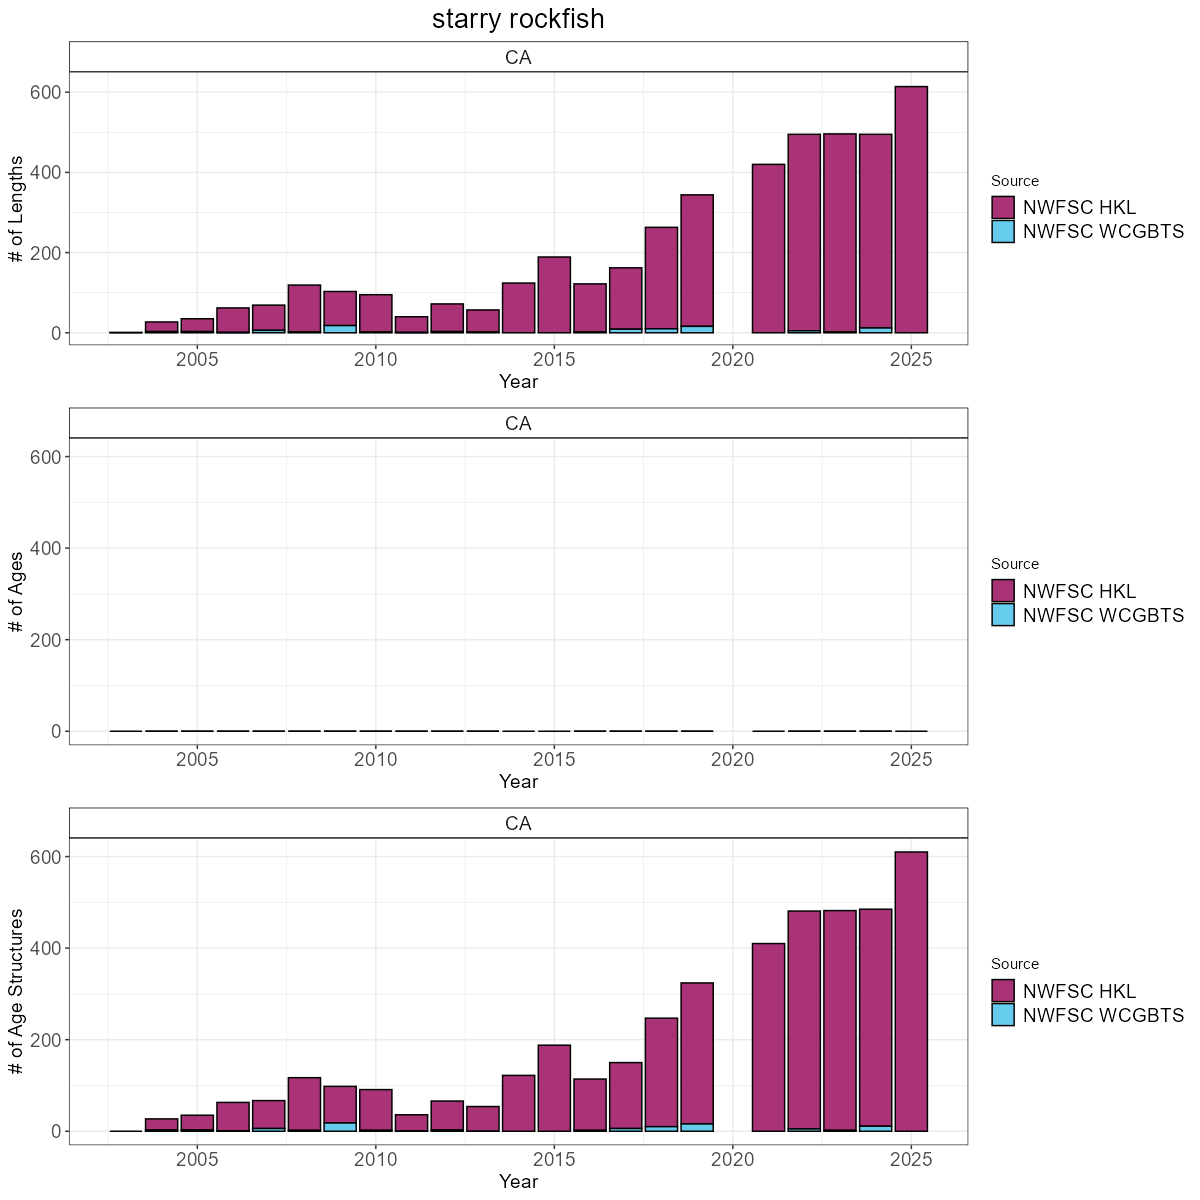
\includegraphics[width=0.95\linewidth,height=\textheight,keepaspectratio]{../plots/state_comparisons/starry_rockfish_state_compositions.png}

}

\caption{Total number of available lengths, read ages, and unread age
structures by data source by year for starry rockfish. Note the y-axis
maximum may differ by data type.}

\end{figure}%

\begin{figure}[H]

{\centering 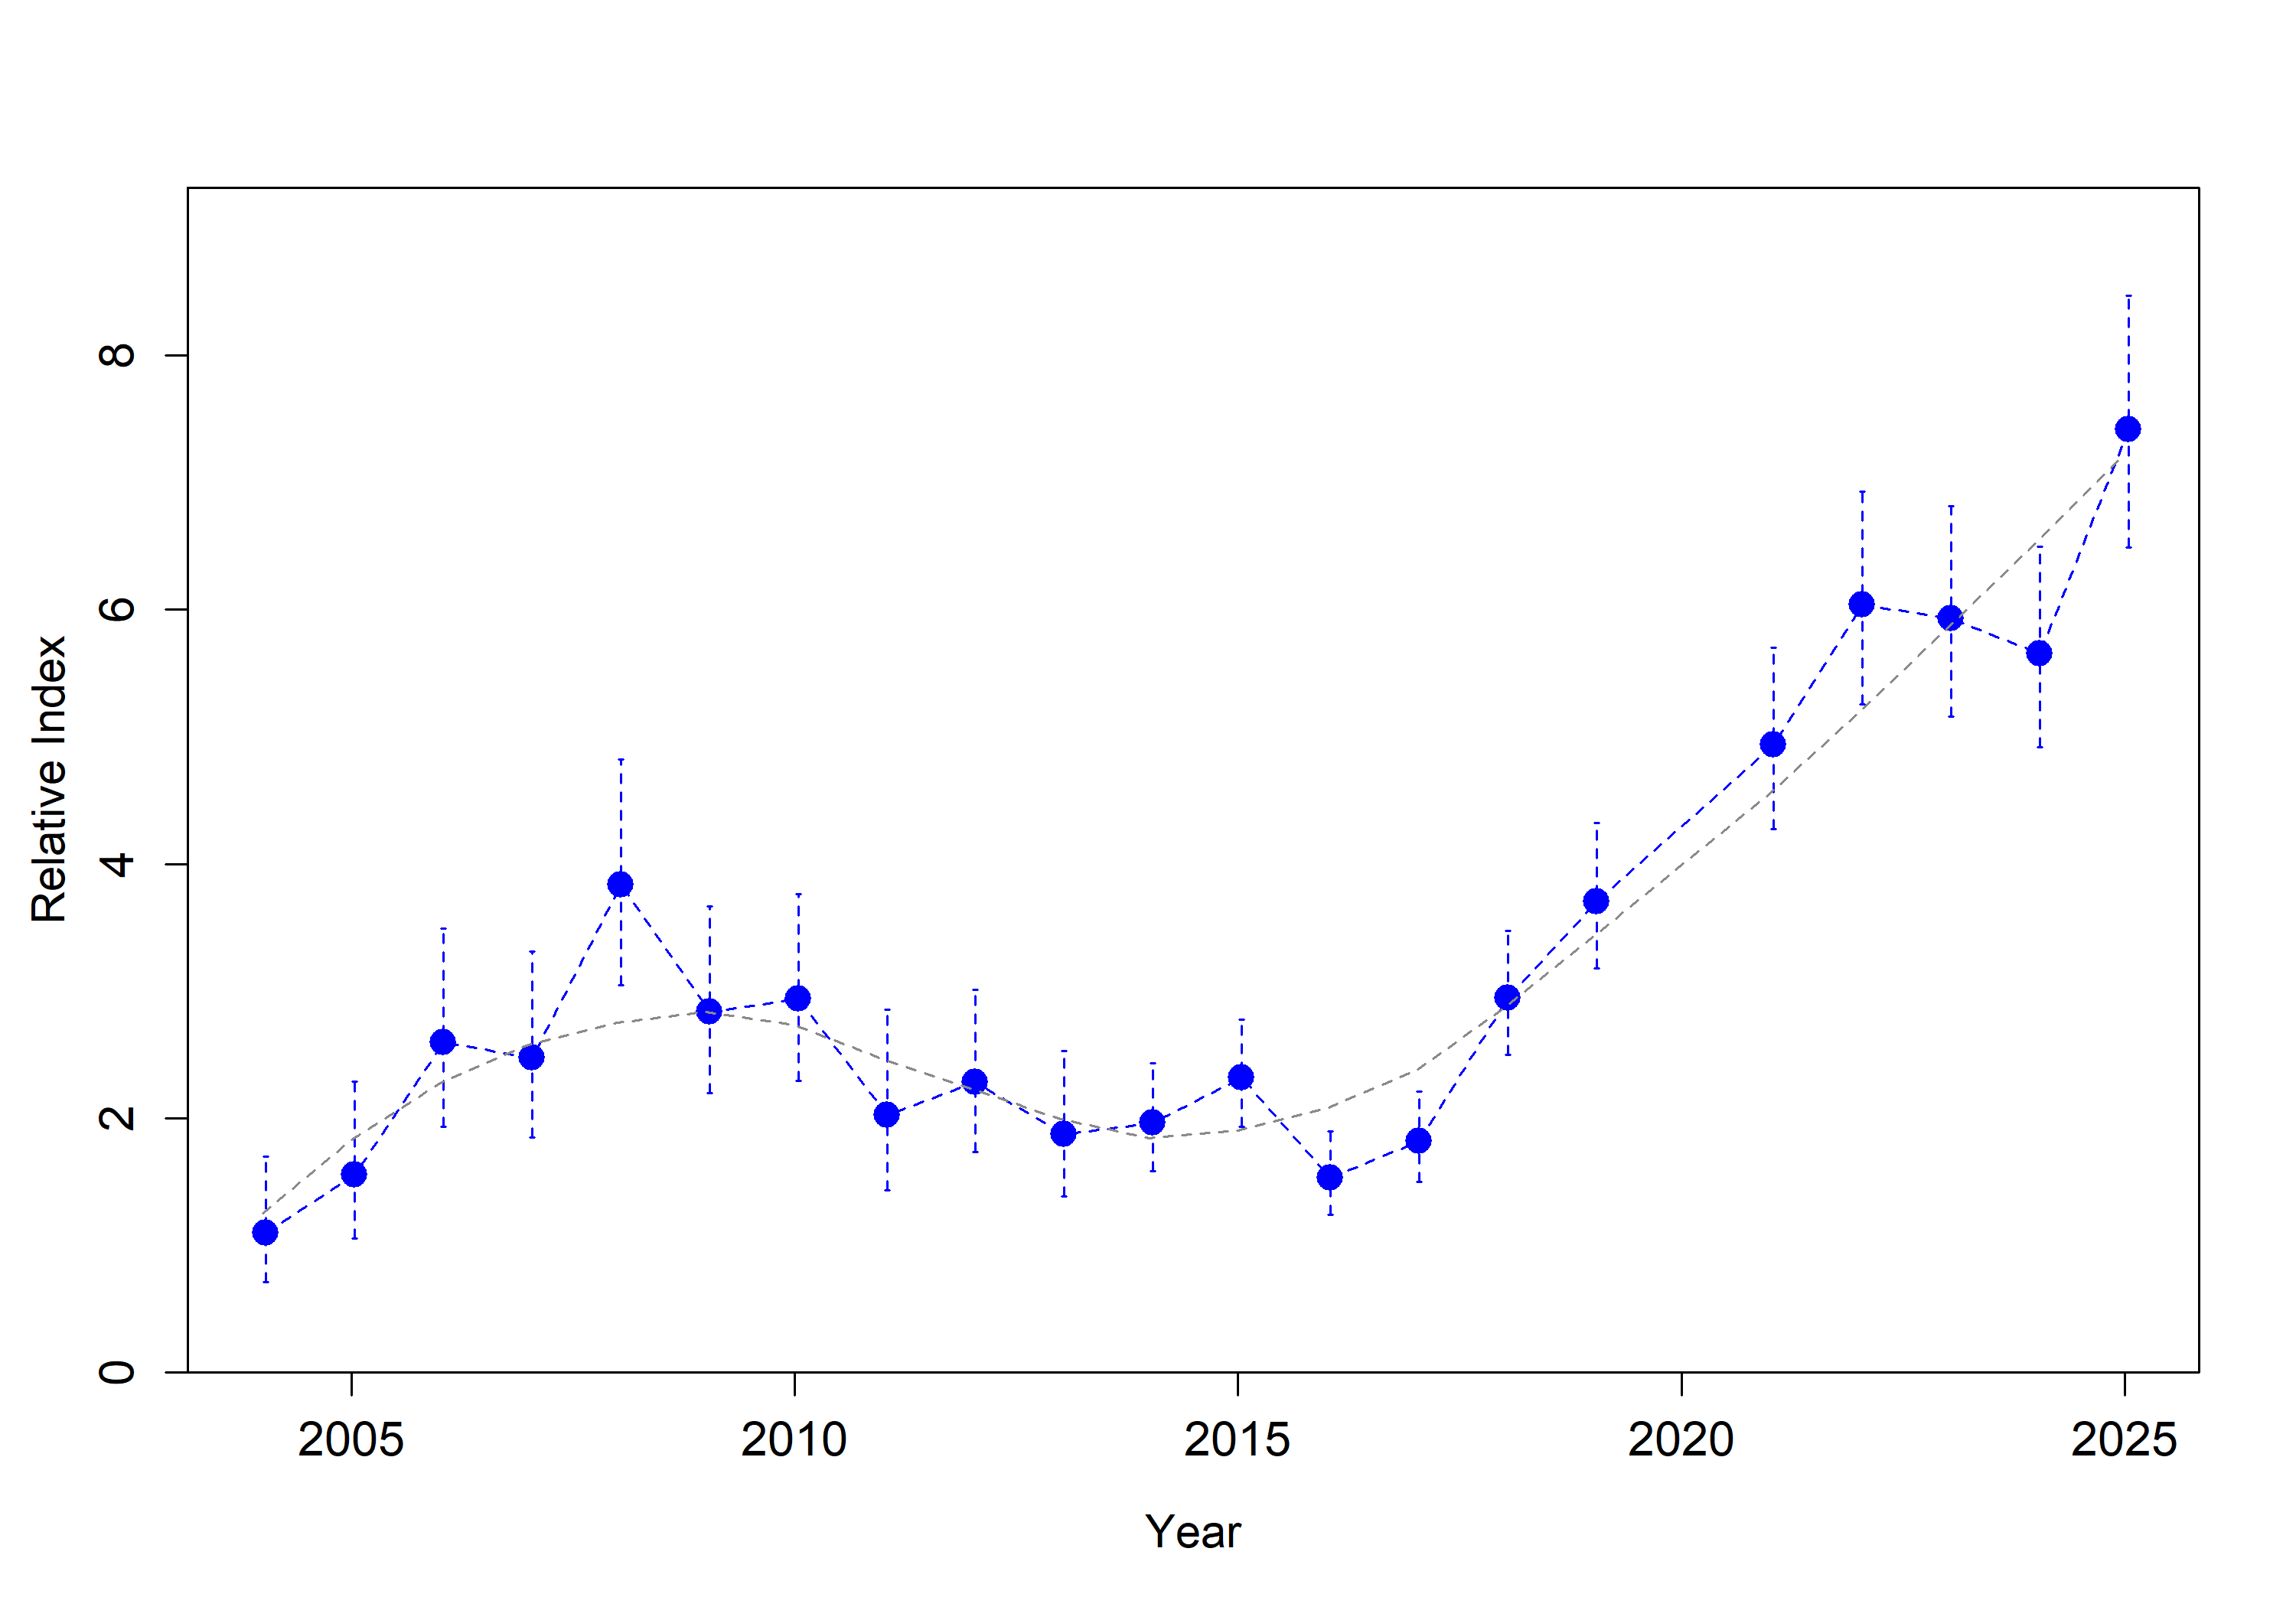
\includegraphics[width=0.95\linewidth,height=\textheight,keepaspectratio]{../plots/hkl_indices/starry rockfish_negbinom index.png}

}

\caption{Estimated relative index of abundance for starry rockfish from
the NWFSC HKLS.}

\end{figure}%

\begin{figure}[H]

{\centering 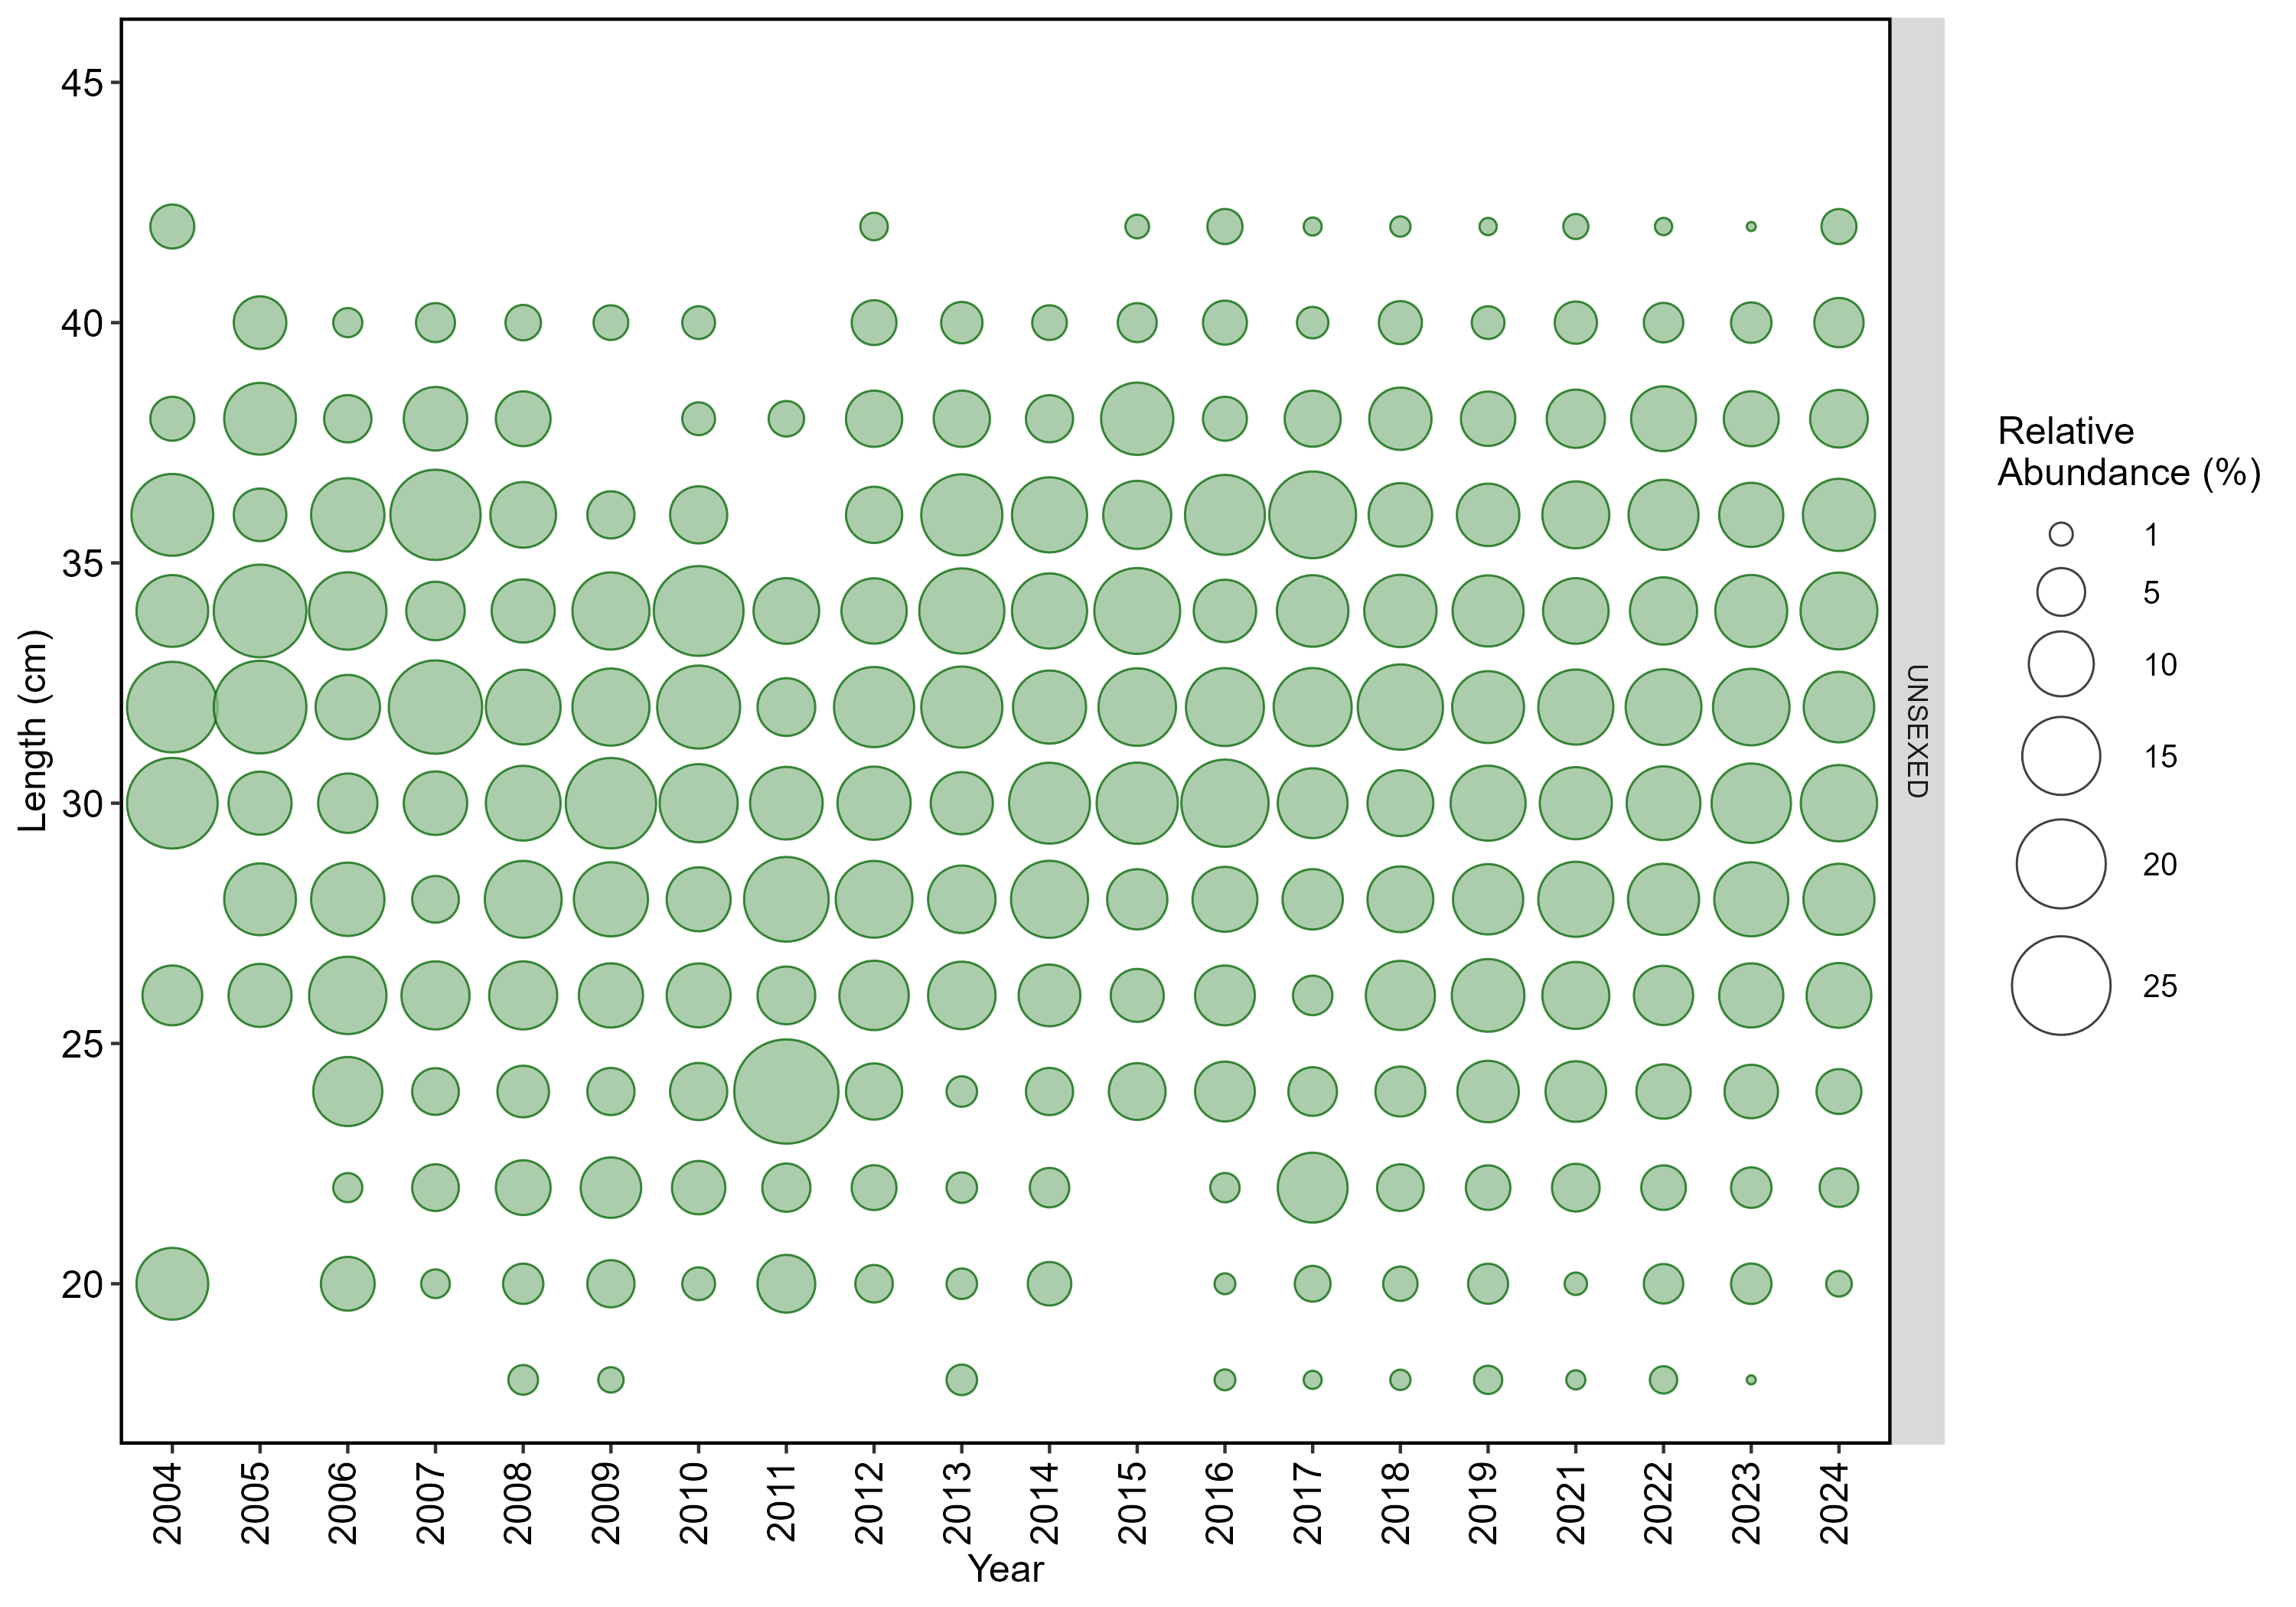
\includegraphics[width=0.95\linewidth,height=\textheight,keepaspectratio]{../plots/hkl_comps/plots/starry rockfish_nwfsc_hkl_length_frequency_sex_0.png}

}

\caption{Length (cm) compostion data from the NWFSC HKLS for starry
rockfish. Size of the circles within a year indicate higher (larger
circles) and lower (smaller circles) proportion observed by length bin.}

\end{figure}%

\newpage{}

\subsection{Stripetail rockfish}\label{stripetail-rockfish}

To date, no assessment or analysis has been conducted on stripetail
rockfish. Across available data, stripetail rockfish have been observed
and sampled by both the NWFSC HKLS and WCGBTS. The NWFSC HKLS observed
stripetail rockfish at an average of 0 sets per year. The NWFSC WCGBTS
observed stripetail rockfish on an average of 140 tows per year. For
this species, a total of 67 maturity samples have been collected
coastwide (regardless of stock area), with 67 read maturities.

\begingroup\fontsize{10}{12}\selectfont
\begingroup\fontsize{10}{12}\selectfont

\begin{longtable}[t]{>{\raggedleft\arraybackslash}p{2cm}>{\raggedleft\arraybackslash}p{3.5cm}>{\raggedleft\arraybackslash}p{2cm}>{\raggedleft\arraybackslash}p{2cm}>{\raggedleft\arraybackslash}p{2cm}}
\caption{\label{tab:unnamed-chunk-670}Total number of available lengths, read ages, and unread age structures by data source and
state for stripetail rockfish.}\\
\toprule
State & Source & Lengths & Ages & Age Structures\\
\midrule
\endfirsthead
\caption[]{Total number of available lengths, read ages, and unread age structures by data source and
state for stripetail rockfish. (\textit{continued)}}\\
\toprule
State & Source & Lengths & Ages & Age Structures\\
\midrule
\endhead

\endfoot
\bottomrule
\endlastfoot
CA & NWFSC HKLS & 3 & 0 & 3\\
CA & NWFSC WCGBTS & 44,050 & 0 & 8,911\\
OR & NWFSC WCGBTS & 9,488 & 0 & 2,374\\
WA & NWFSC WCGBTS & 1,589 & 0 & 523\\*
\end{longtable}
\endgroup{}
\endgroup{}

\begin{figure}[H]

{\centering 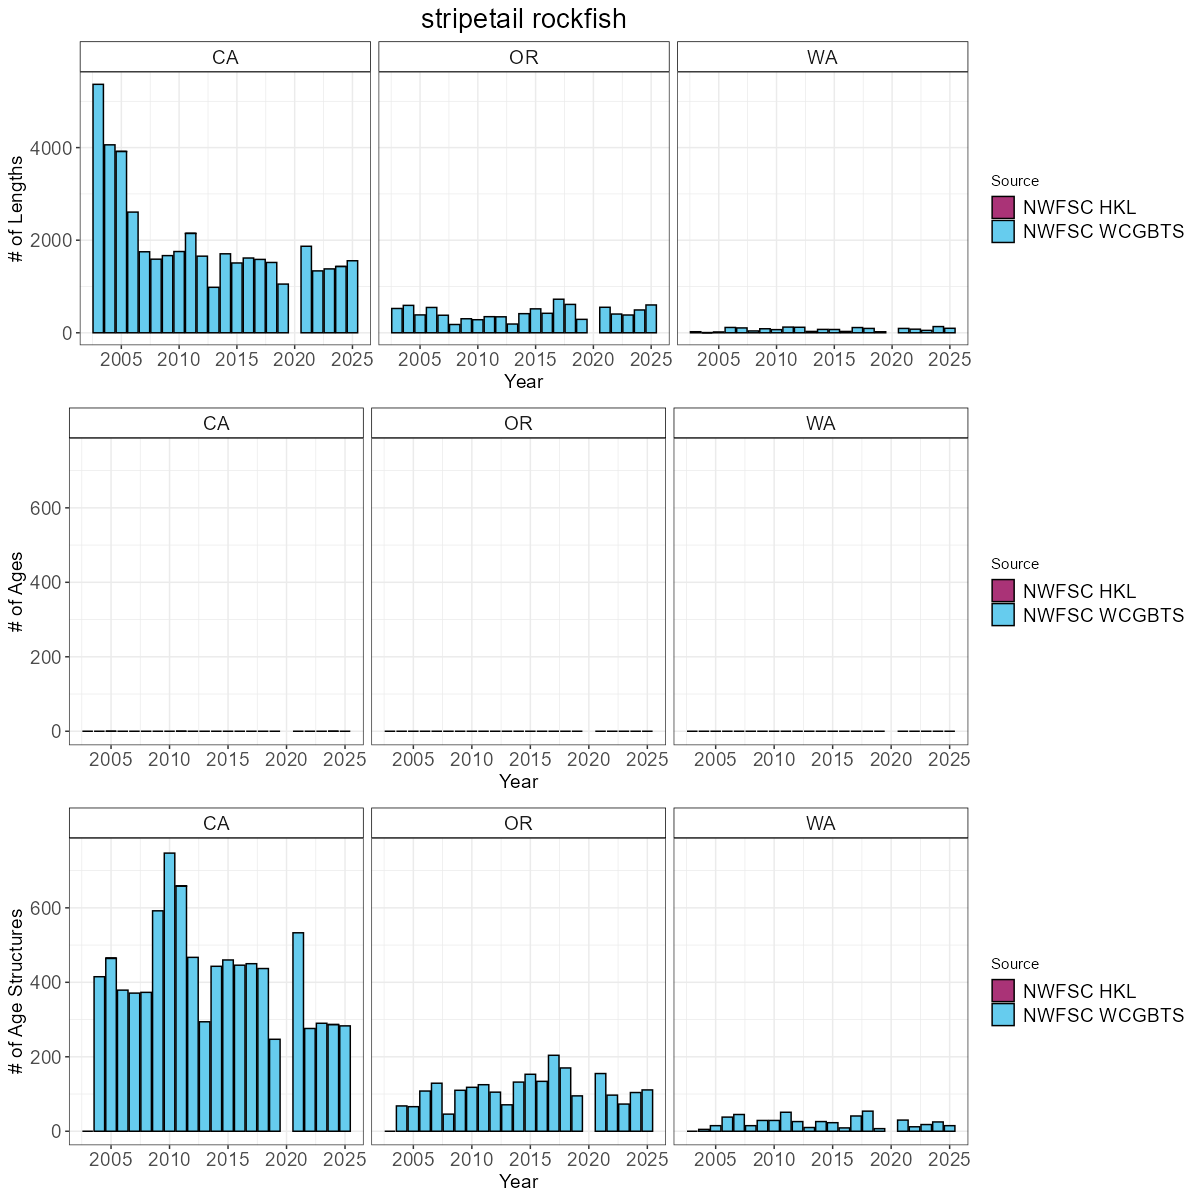
\includegraphics[width=0.95\linewidth,height=\textheight,keepaspectratio]{../plots/state_comparisons/stripetail_rockfish_state_compositions.png}

}

\caption{Total number of available lengths, read ages, and unread age
structures by data source by year for stripetail rockfish. Note the
y-axis maximum may differ by data type.}

\end{figure}%

\begin{figure}[H]

{\centering 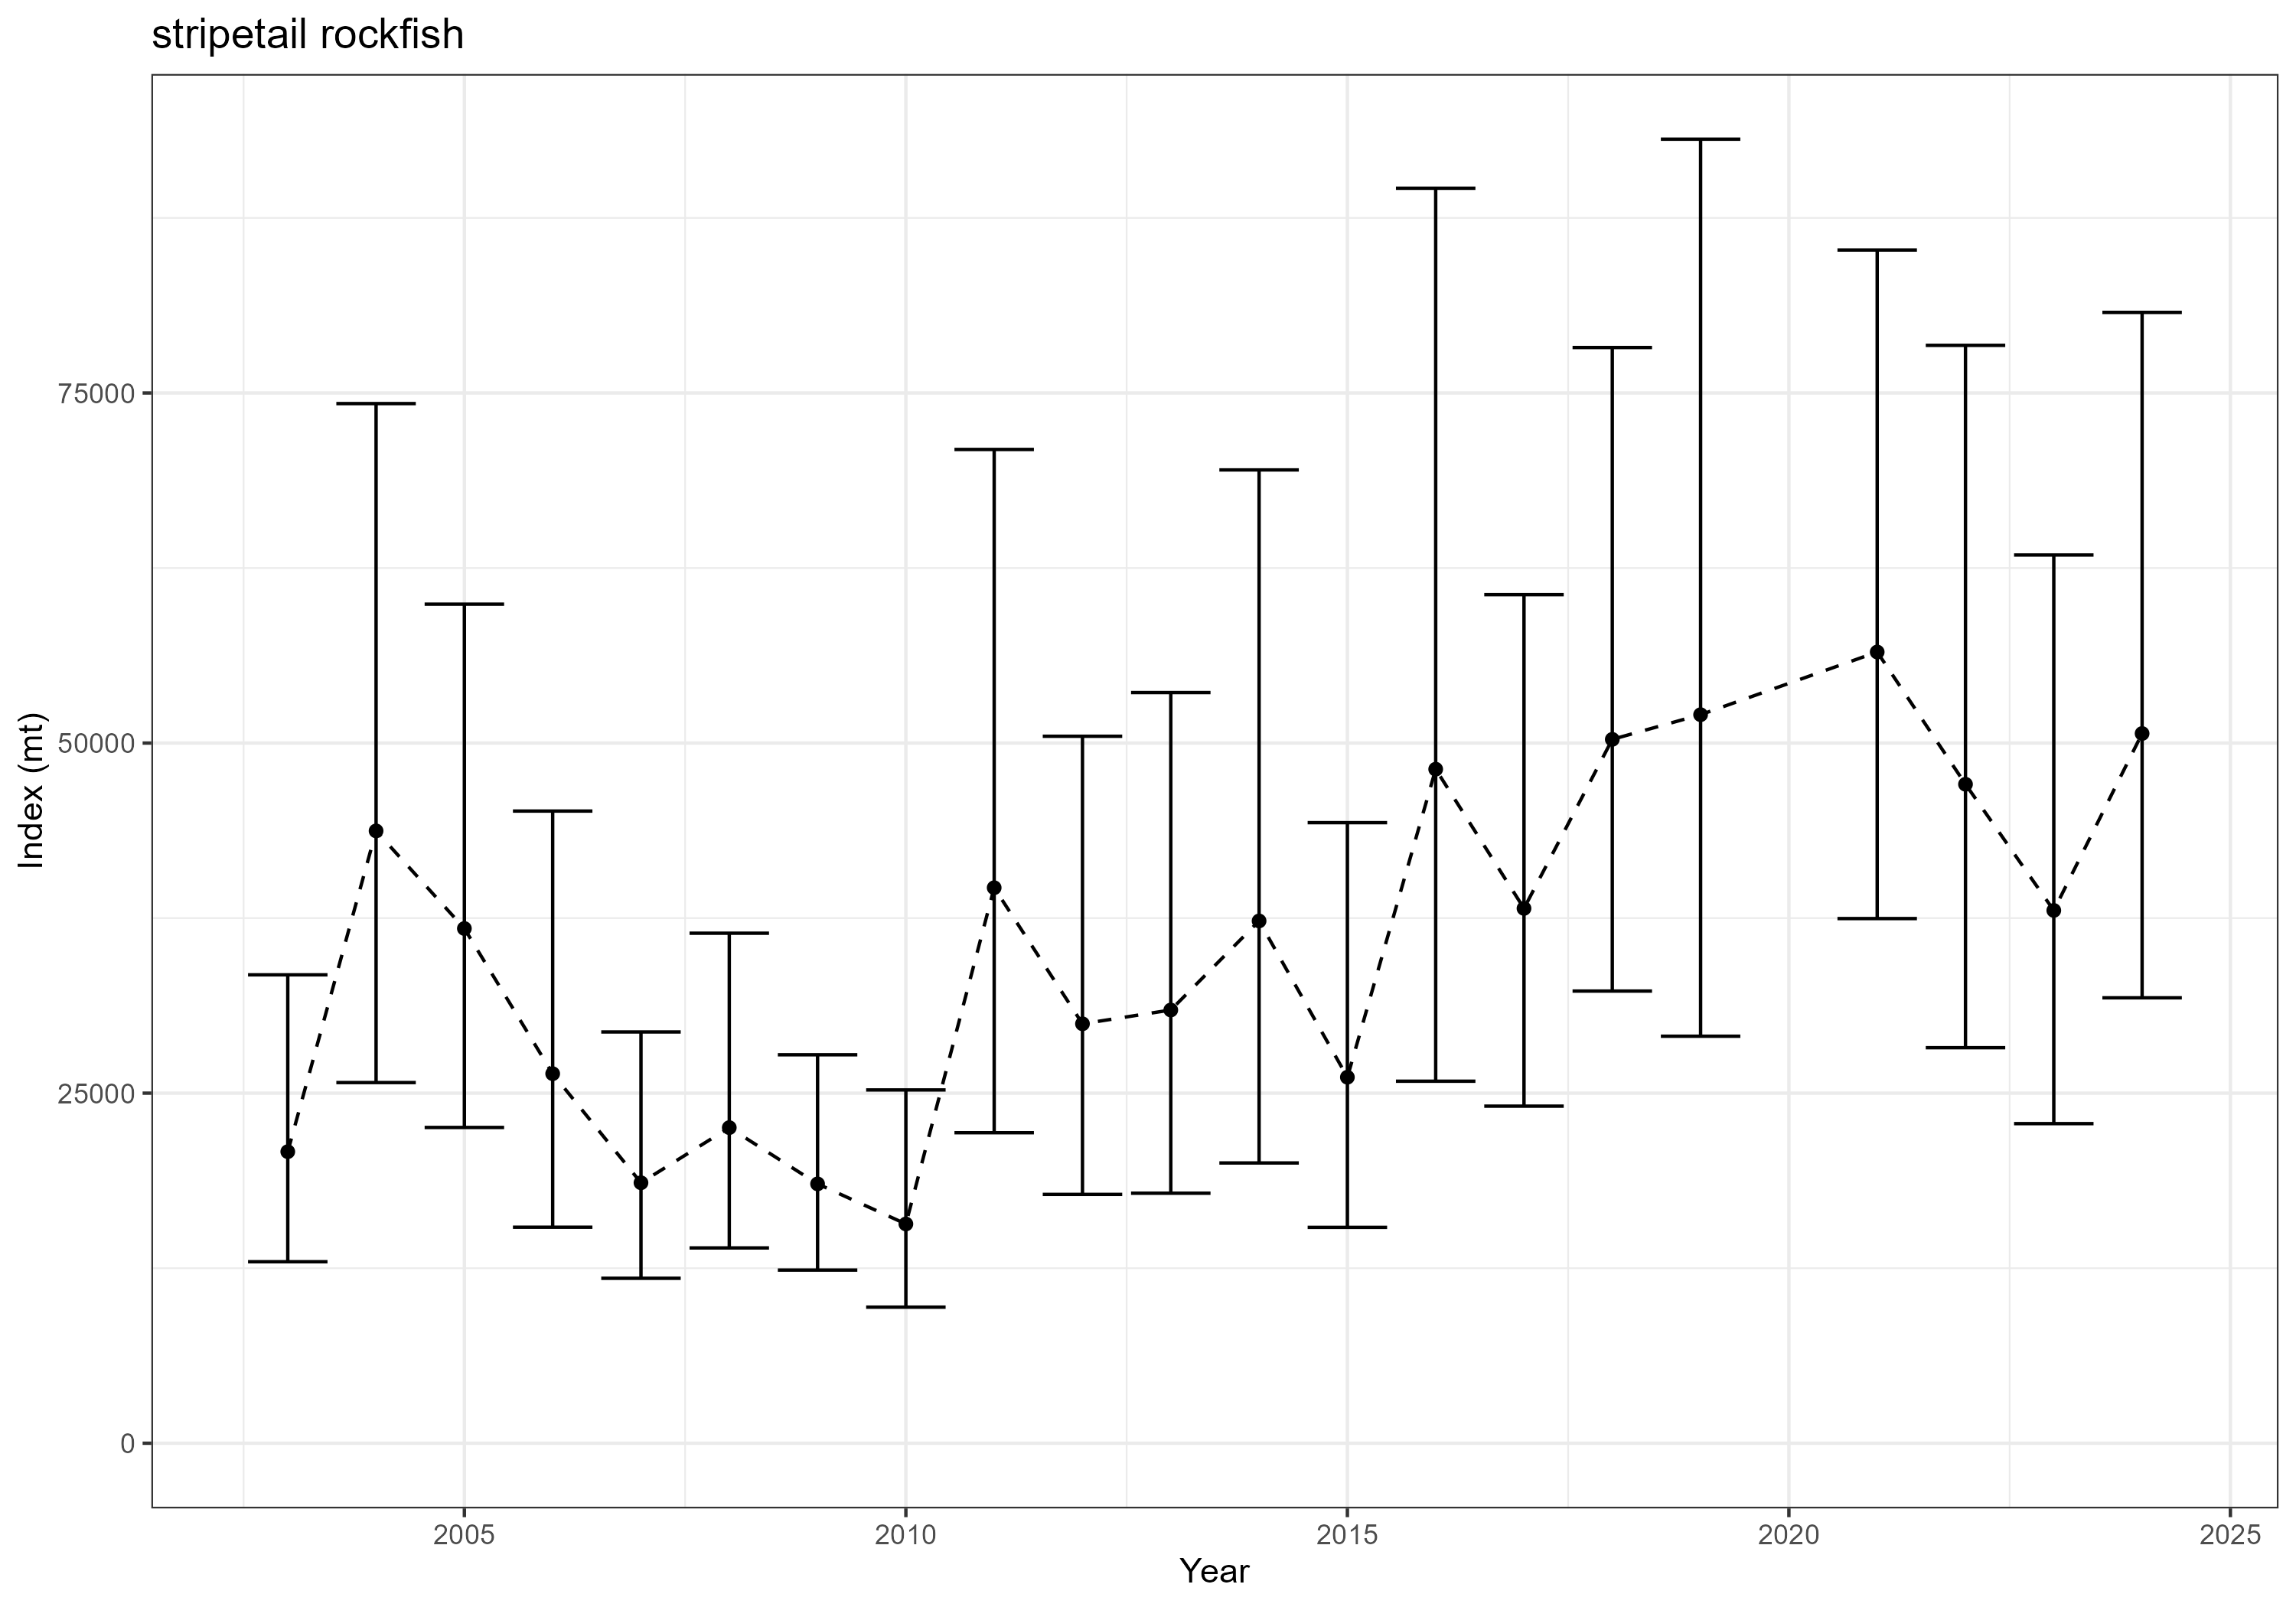
\includegraphics[width=0.95\linewidth,height=\textheight,keepaspectratio]{../plots/wcgbts_indices/stripetail_rockfish_index.png}

}

\caption{Estimated relative index of abundance for stripetail rockfish
from the NWFSC WCGBTS.}

\end{figure}%

\begin{figure}[H]

{\centering 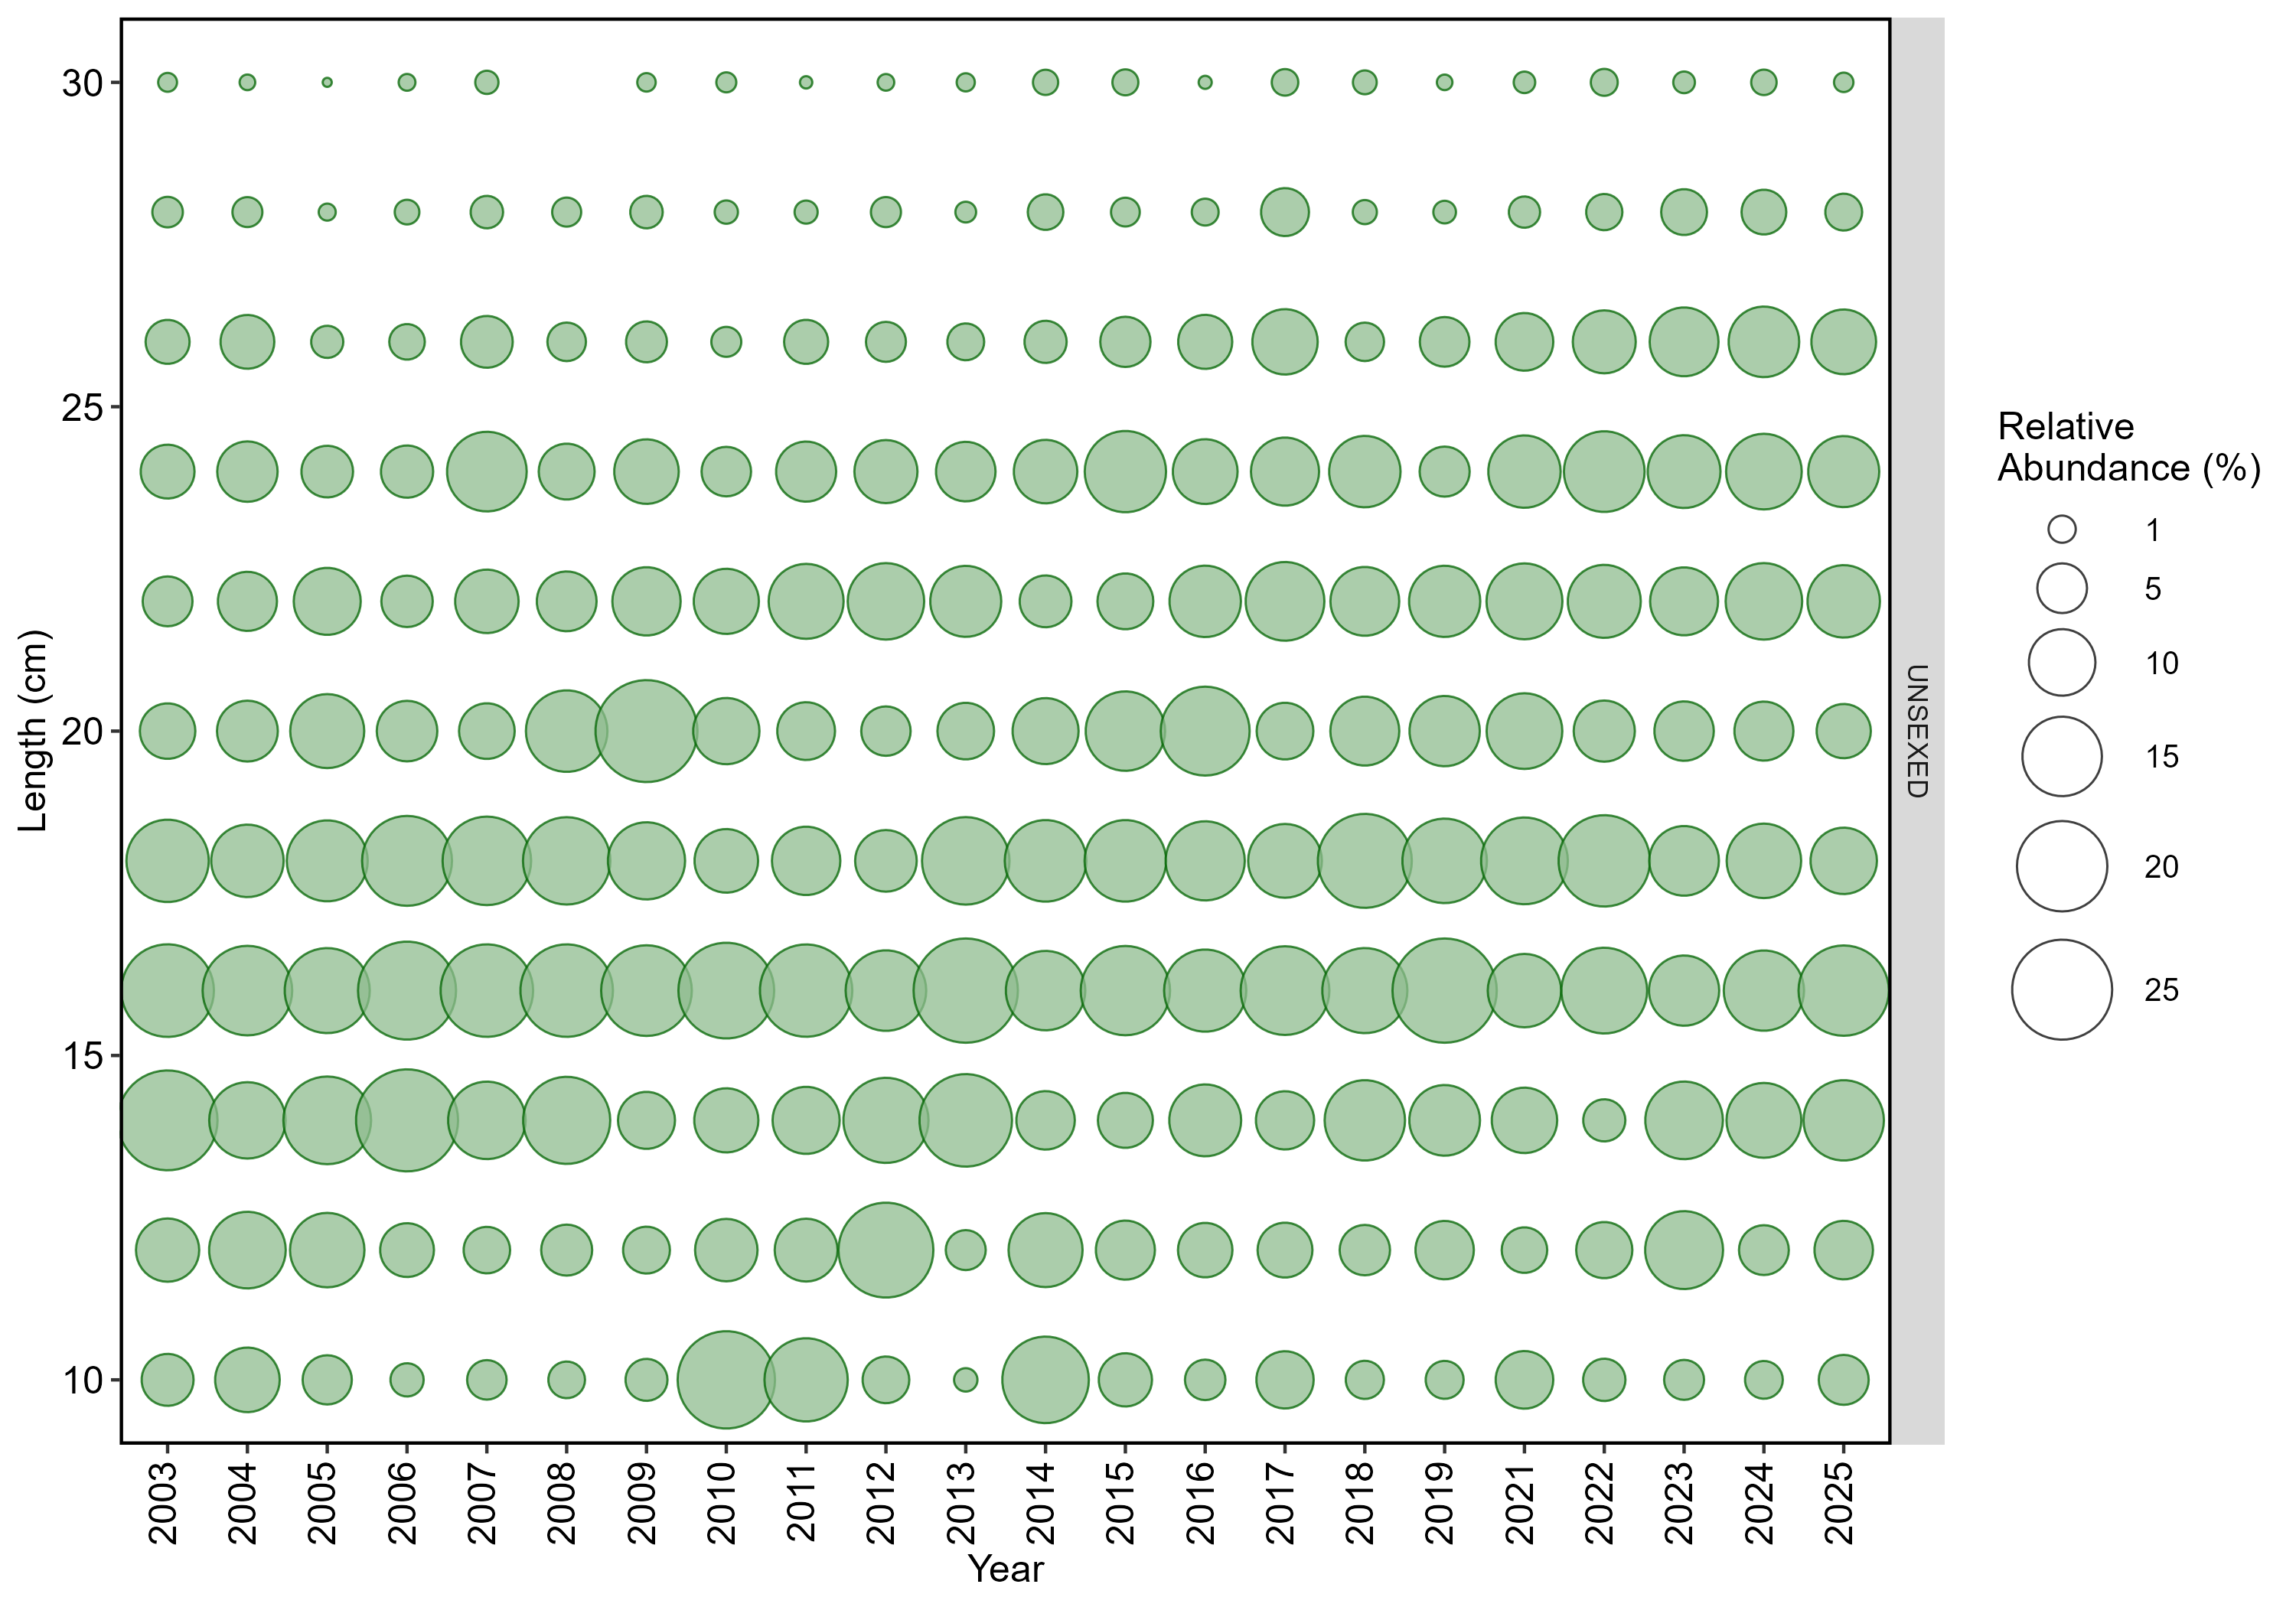
\includegraphics[width=0.95\linewidth,height=\textheight,keepaspectratio]{../plots/wcgbts_comps/plots/stripetail rockfish_length_frequency_sex_0.png}

}

\caption{Length (cm) compostion data from the NWFSC WCGBTS for
stripetail rockfish. Size of the circles within a year indicate higher
(larger circles) and lower (smaller circles) proportion observed by
length bin.}

\end{figure}%

\newpage{}

\subsection{Vermilion and sunset
rockfish}\label{vermilion-and-sunset-rockfish}

The most recent assessment of vermilion and sunset rockfish was a
benchmark assessment conducted in 2021. Across available data, vermilion
and sunset rockfish have been observed and sampled by both the NWFSC
HKLS and WCGBTS. The NWFSC HKLS observed vermilion and sunset rockfish
at an average of 114 sets per year. The NWFSC WCGBTS observed vermilion
and sunset rockfish on an average of 2 tows per year. For this species,
a total of 1728 maturity samples have been collected coastwide
(regardless of stock area), with 1405 read maturities.

\begingroup\fontsize{10}{12}\selectfont
\begingroup\fontsize{10}{12}\selectfont

\begin{longtable}[t]{>{\raggedleft\arraybackslash}p{2cm}>{\raggedleft\arraybackslash}p{3.5cm}>{\raggedleft\arraybackslash}p{2cm}>{\raggedleft\arraybackslash}p{2cm}>{\raggedleft\arraybackslash}p{2cm}}
\caption{\label{tab:unnamed-chunk-687}Total number of available lengths, read ages, and unread age structures by data source and
state for vermilion and sunset rockfish.}\\
\toprule
State & Source & Lengths & Ages & Age Structures\\
\midrule
\endfirsthead
\caption[]{Total number of available lengths, read ages, and unread age structures by data source and
state for vermilion and sunset rockfish. (\textit{continued)}}\\
\toprule
State & Source & Lengths & Ages & Age Structures\\
\midrule
\endhead

\endfoot
\bottomrule
\endlastfoot
CA & NWFSC HKLS & 34,481 & 9,334 & 13,420\\
CA & NWFSC WCGBTS & 595 & 303 & 41\\*
\end{longtable}
\endgroup{}
\endgroup{}

\begin{figure}[H]

{\centering 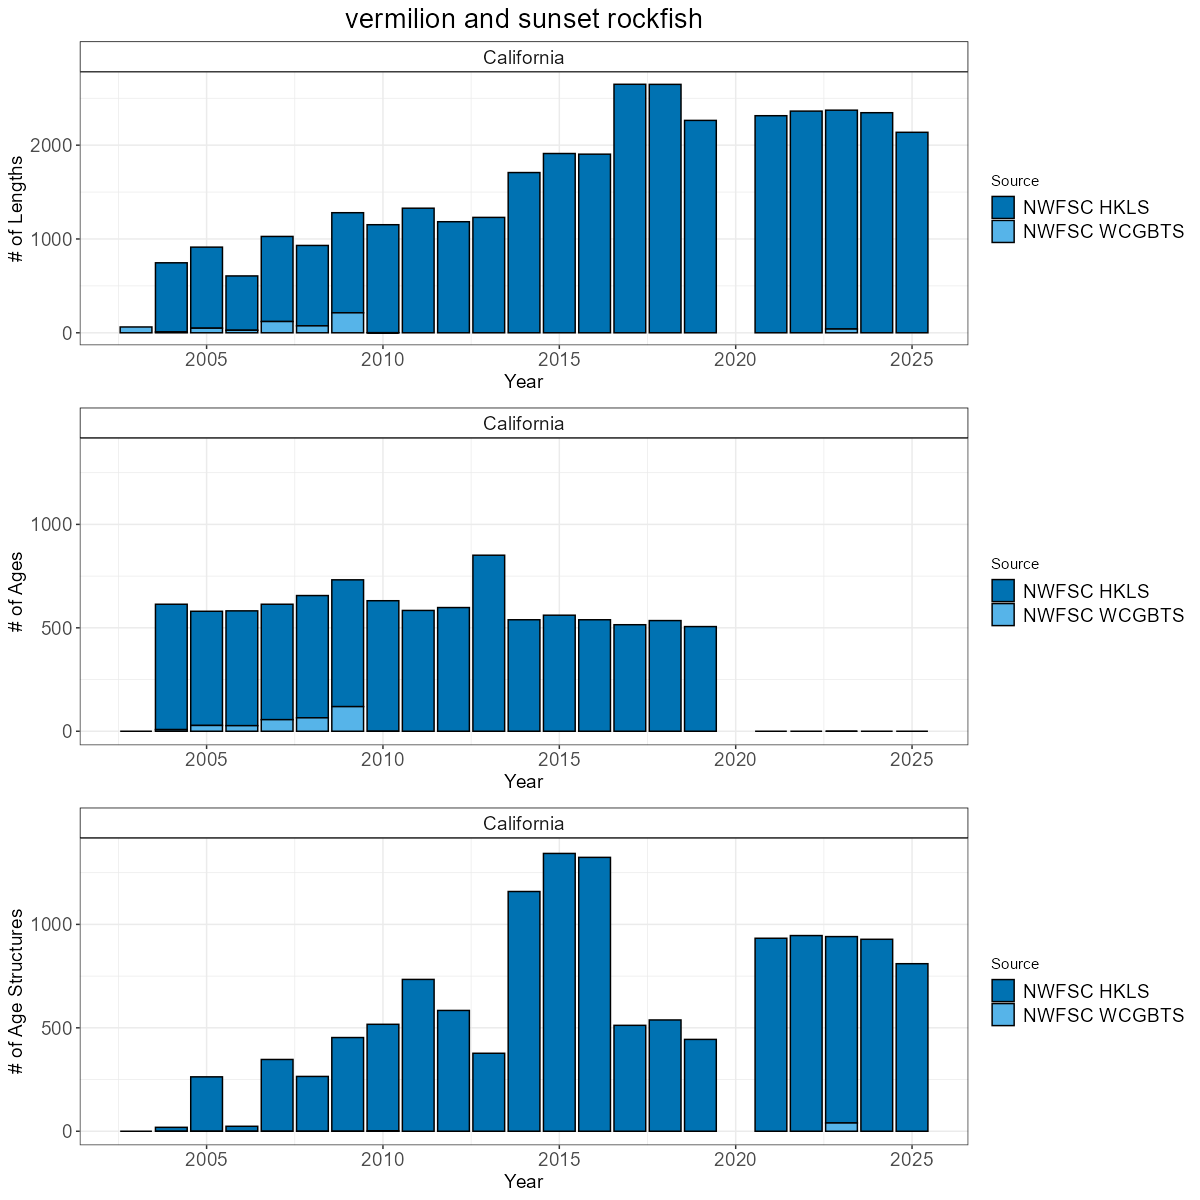
\includegraphics[width=0.95\linewidth,height=\textheight,keepaspectratio]{../plots/state_comparisons/vermilion_and_sunset_rockfish_state_compositions.png}

}

\caption{Total number of available lengths, read ages, and unread age
structures by data source by year for vermilion and sunset rockfish.
Note the y-axis maximum may differ by data type.}

\end{figure}%

\begin{figure}[H]

{\centering 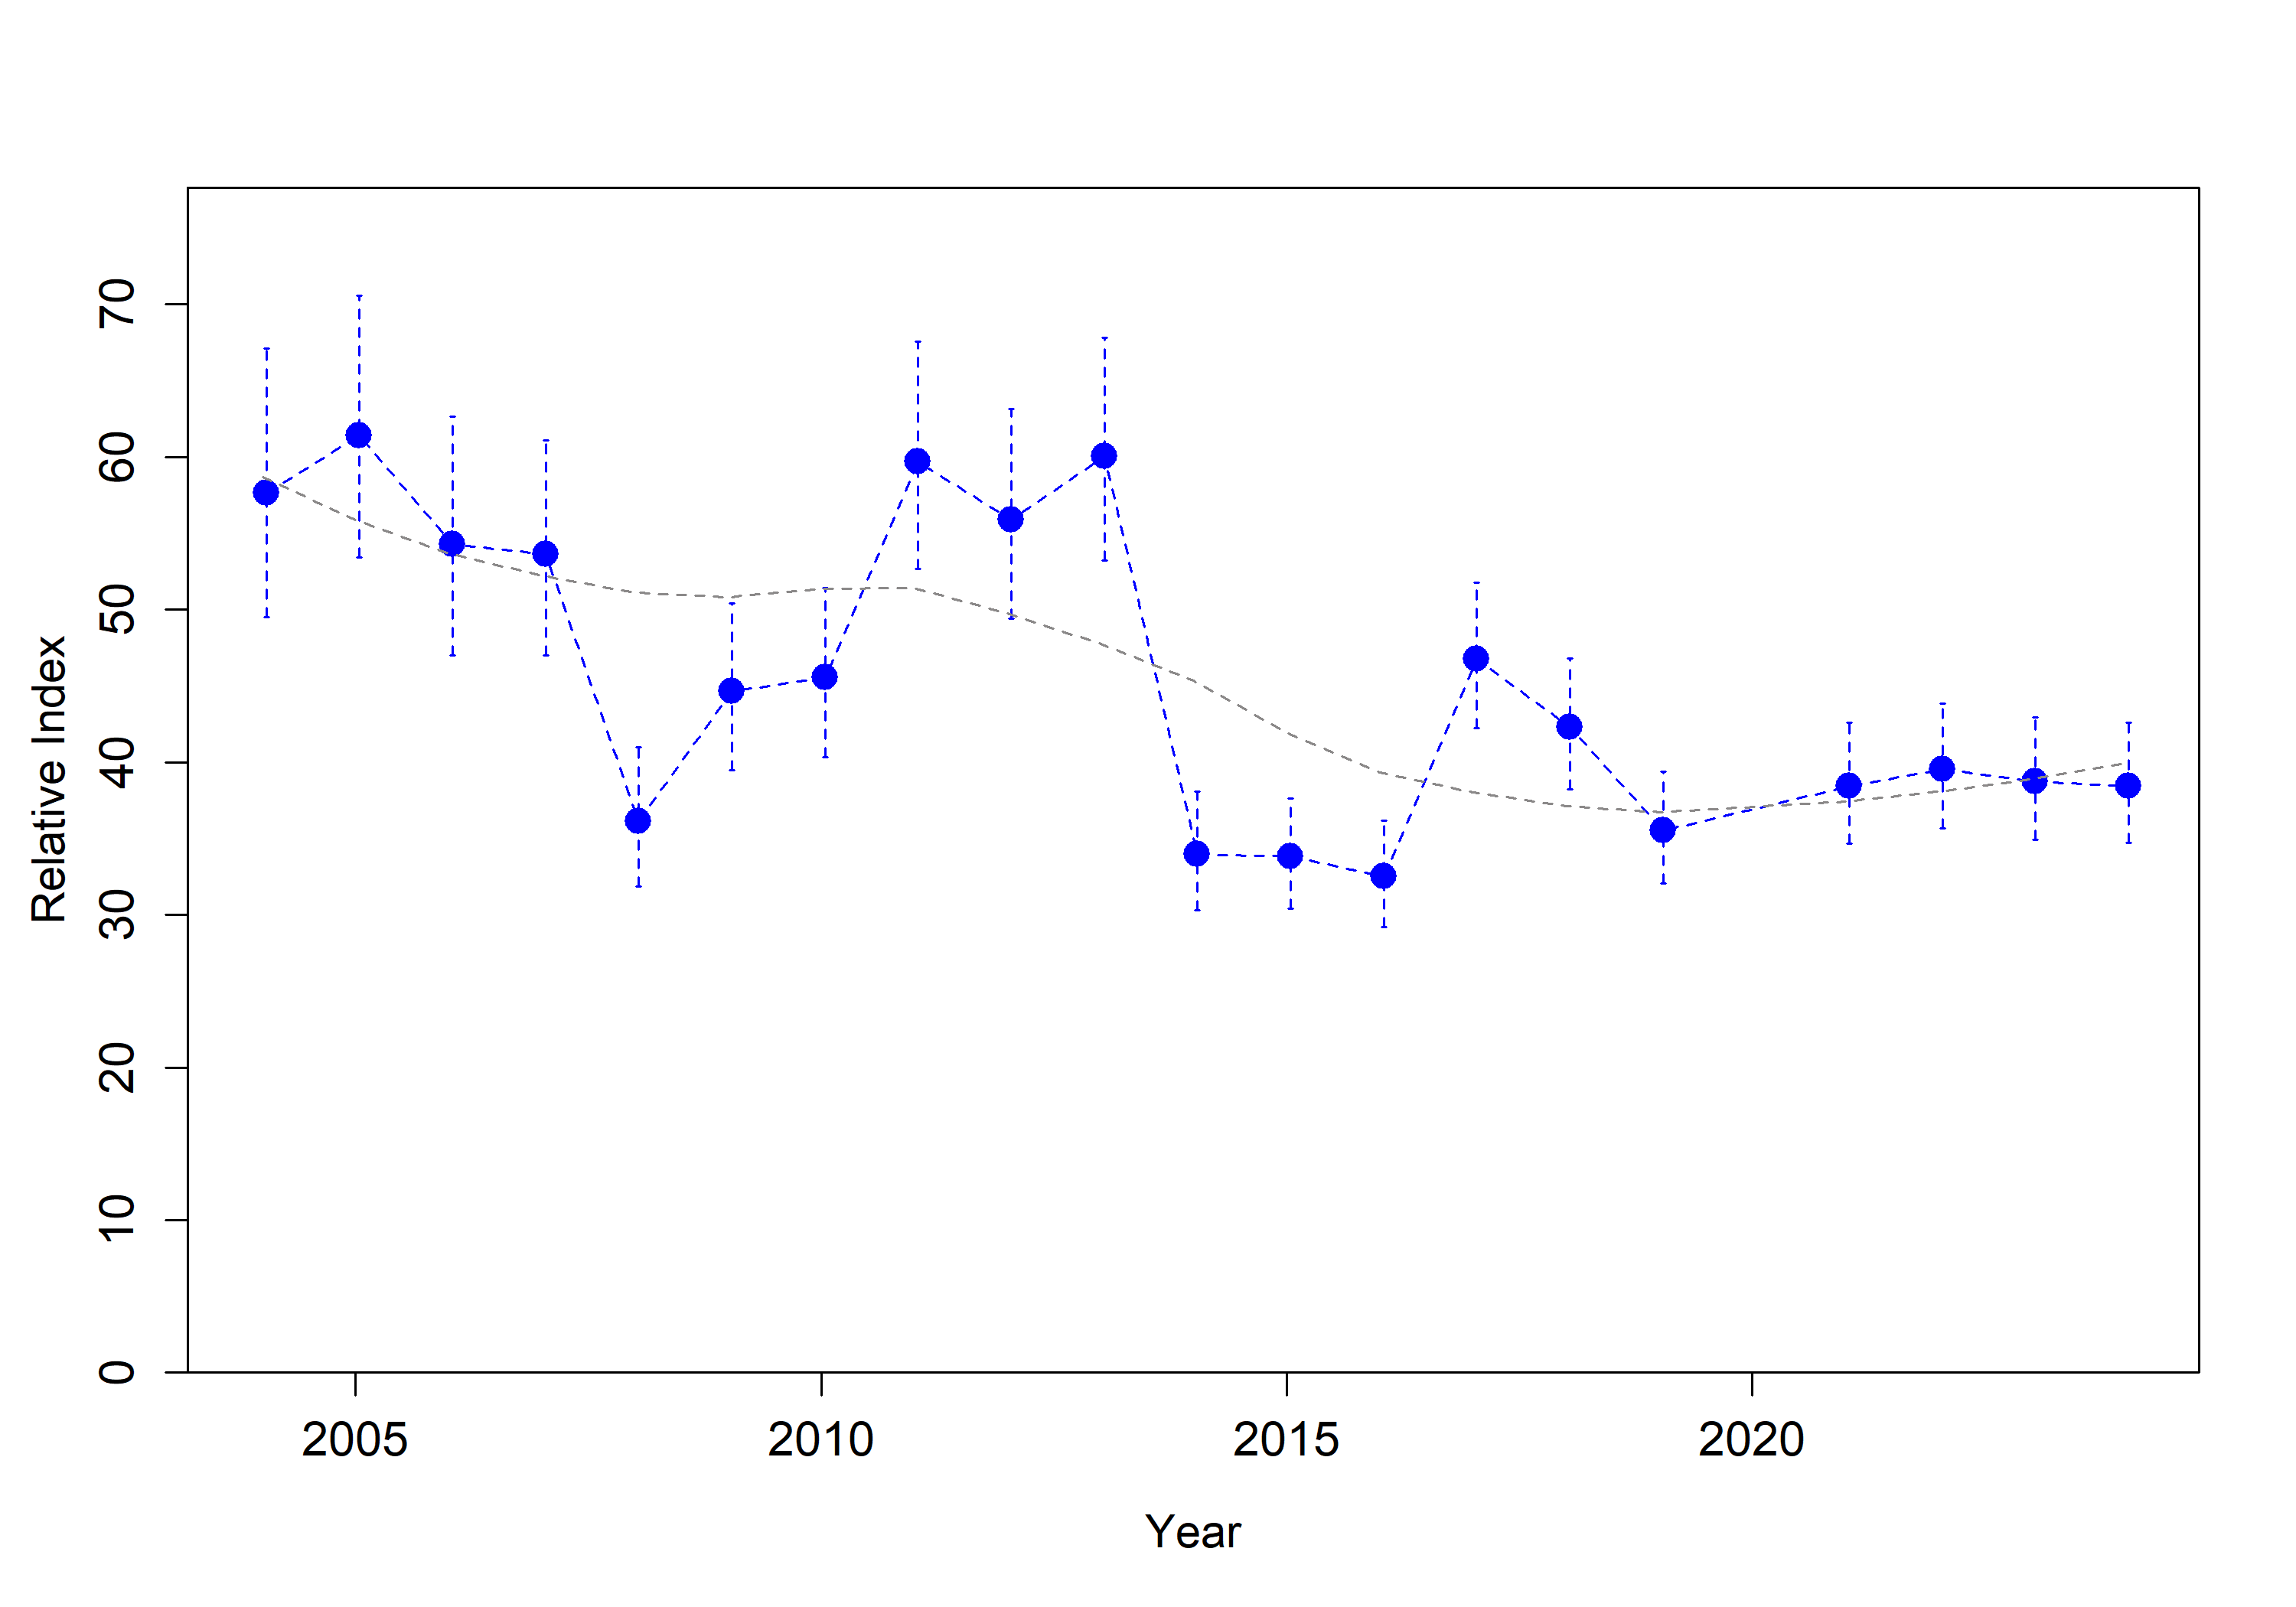
\includegraphics[width=0.95\linewidth,height=\textheight,keepaspectratio]{../plots/hkl_indices/vermilion and sunset rockfish_negbinom index.png}

}

\caption{Estimated relative index of abundance for vermilion and sunset
rockfish from the NWFSC HKLS.}

\end{figure}%

\begin{figure}[H]

{\centering 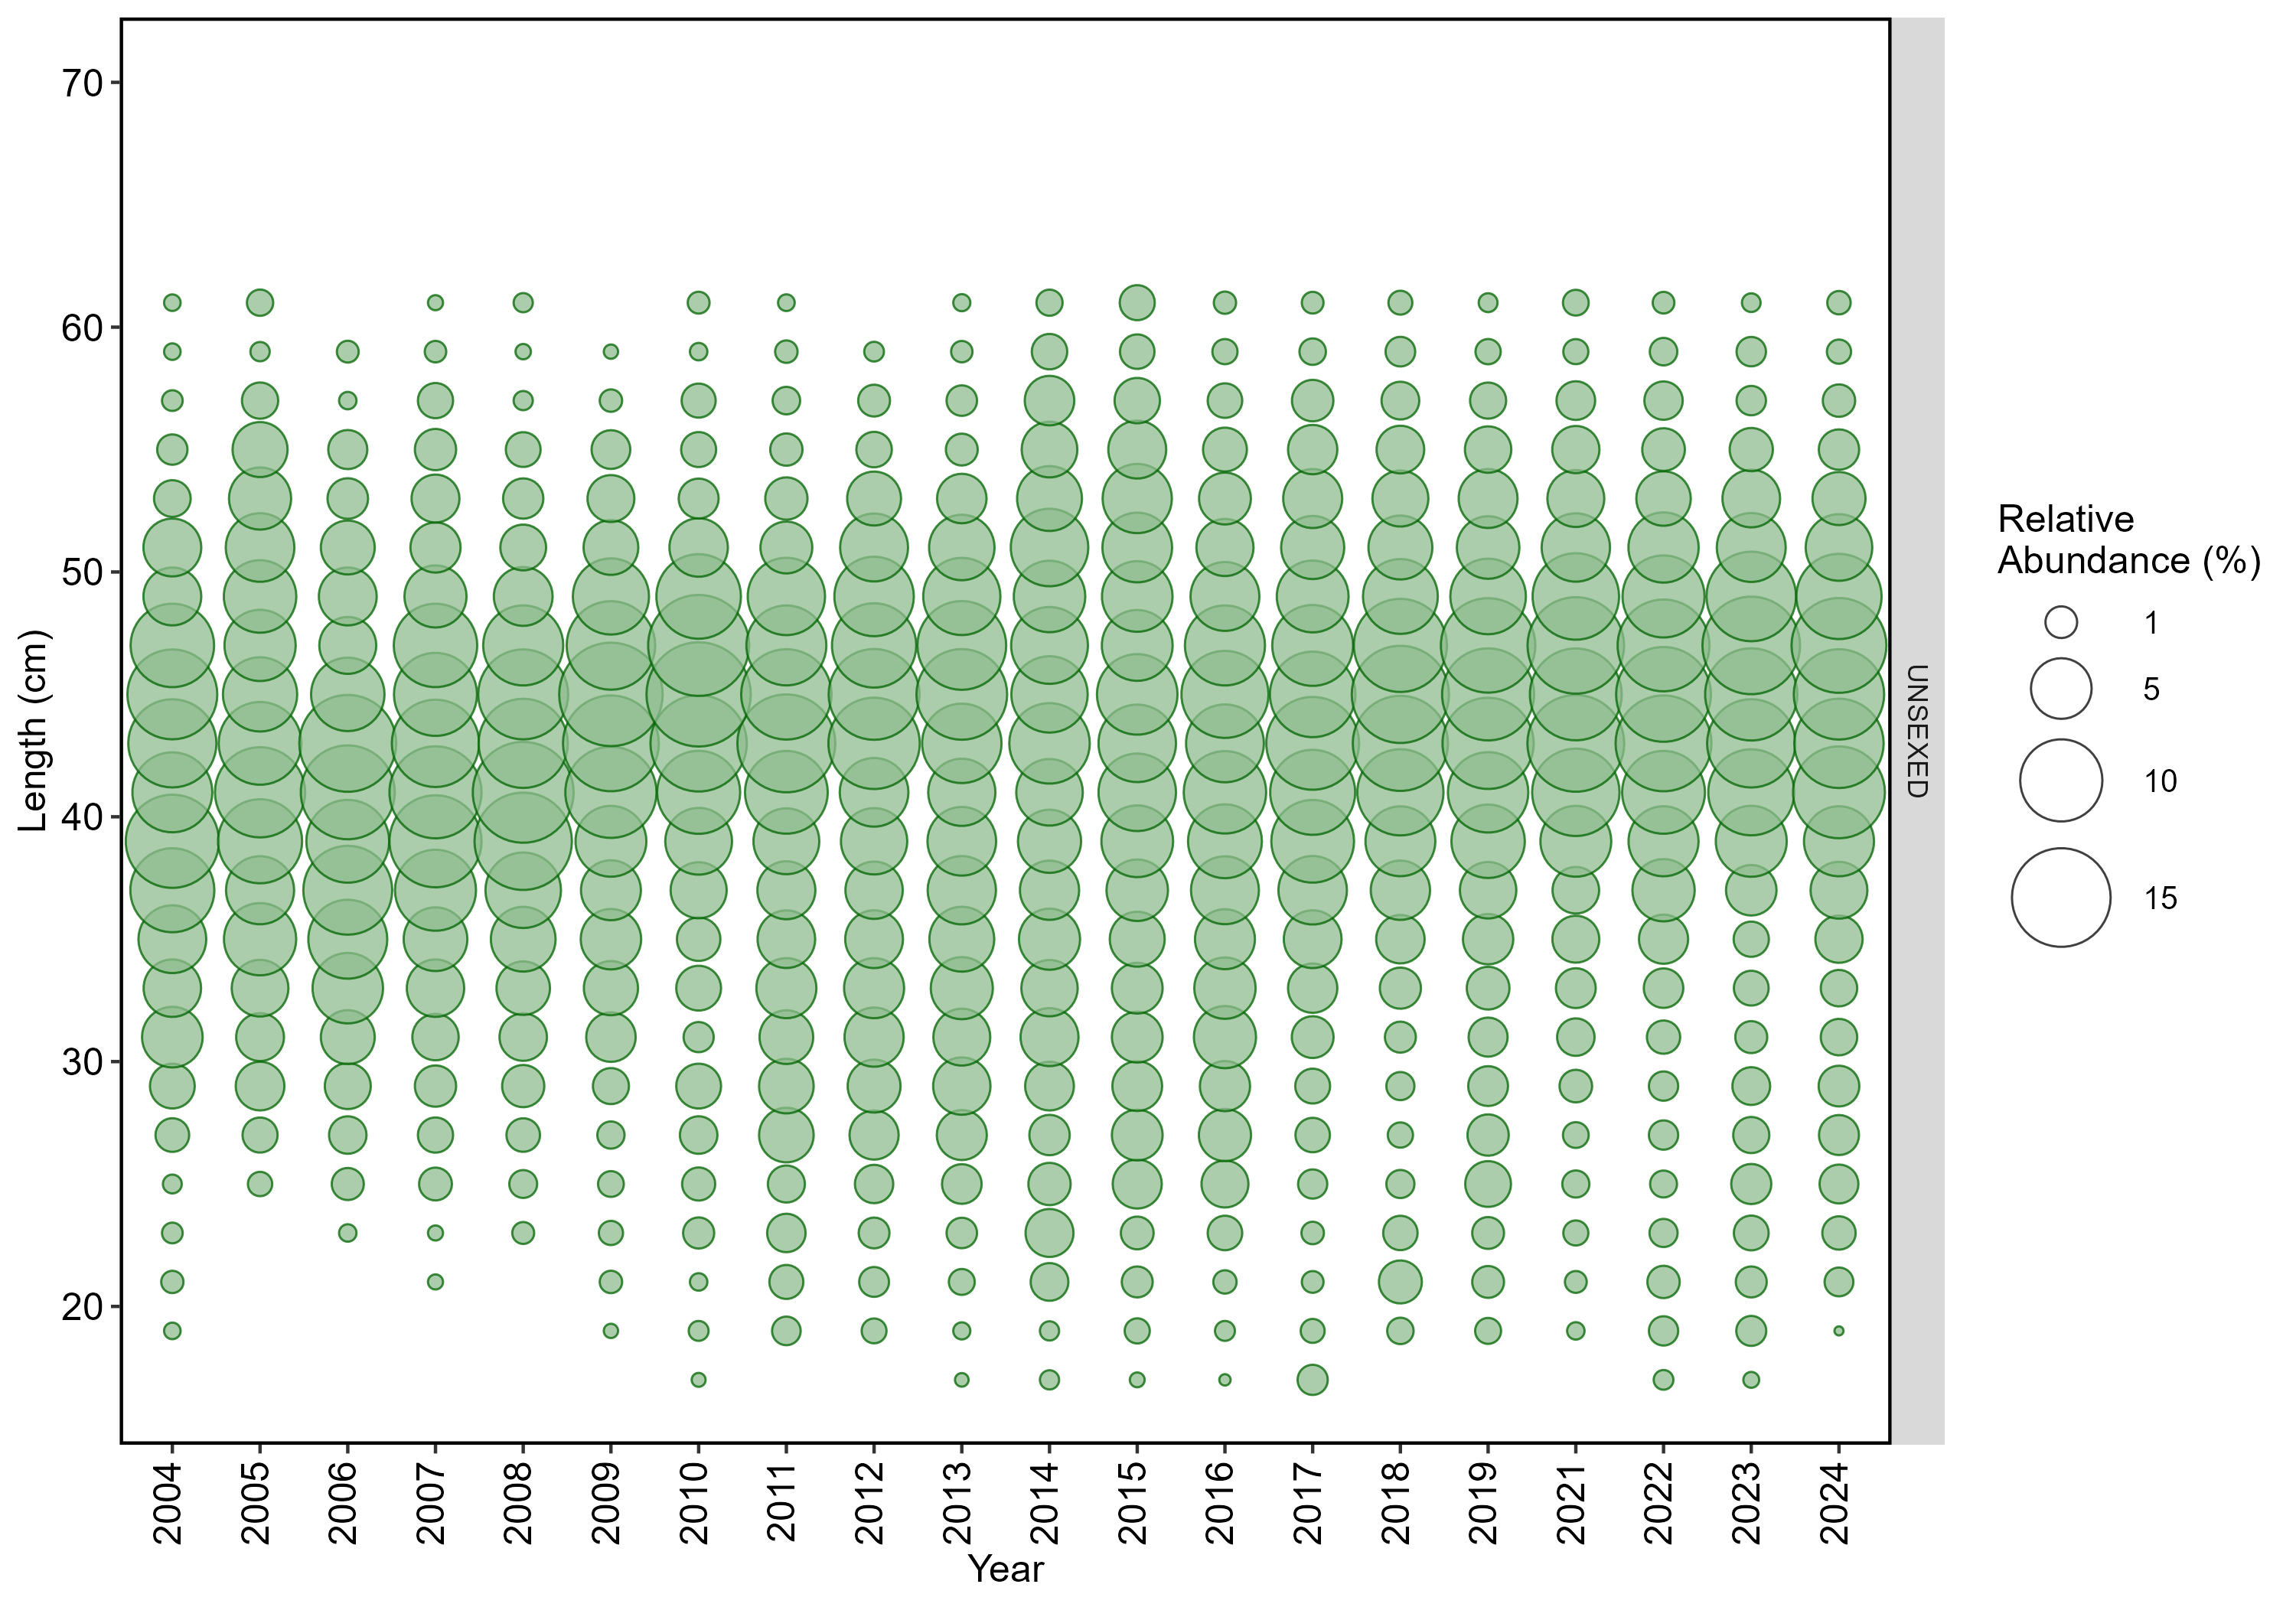
\includegraphics[width=0.95\linewidth,height=\textheight,keepaspectratio]{../plots/hkl_comps/plots/vermilion and sunset rockfish_nwfsc_hkl_length_frequency_sex_0.png}

}

\caption{Length (cm) compostion data from the NWFSC HKLS for vermilion
and sunset rockfish. Size of the circles within a year indicate higher
(larger circles) and lower (smaller circles) proportion observed by
length bin.}

\end{figure}%

\newpage{}

\subsection{Widow rockfish}\label{widow-rockfish}

The most recent assessment of widow rockfish was an update assessment
conducted in 2025. Across available data, widow rockfish have been
observed and sampled by both the NWFSC HKLS and WCGBTS. The NWFSC HKLS
observed widow rockfish at an average of 15 sets per year. The NWFSC
WCGBTS observed widow rockfish on an average of 25 tows per year. For
this species, a total of 322 maturity samples have been collected
coastwide (regardless of stock area), with 92 read maturities.

\begingroup\fontsize{10}{12}\selectfont
\begingroup\fontsize{10}{12}\selectfont

\begin{longtable}[t]{>{\raggedleft\arraybackslash}p{2cm}>{\raggedleft\arraybackslash}p{3.5cm}>{\raggedleft\arraybackslash}p{2cm}>{\raggedleft\arraybackslash}p{2cm}>{\raggedleft\arraybackslash}p{2cm}}
\caption{\label{tab:unnamed-chunk-704}Total number of available lengths, read ages, and unread age structures by data source and
state for widow rockfish.}\\
\toprule
State & Source & Lengths & Ages & Age Structures\\
\midrule
\endfirsthead
\caption[]{Total number of available lengths, read ages, and unread age structures by data source and
state for widow rockfish. (\textit{continued)}}\\
\toprule
State & Source & Lengths & Ages & Age Structures\\
\midrule
\endhead

\endfoot
\bottomrule
\endlastfoot
CA & NWFSC HKLS & 940 & 0 & 917\\
CA & NWFSC WCGBTS & 2,149 & 1,363 & 108\\
OR & NWFSC WCGBTS & 2,195 & 1,417 & 44\\
WA & NWFSC WCGBTS & 923 & 520 & 6\\*
\end{longtable}
\endgroup{}
\endgroup{}

\begin{figure}[H]

{\centering 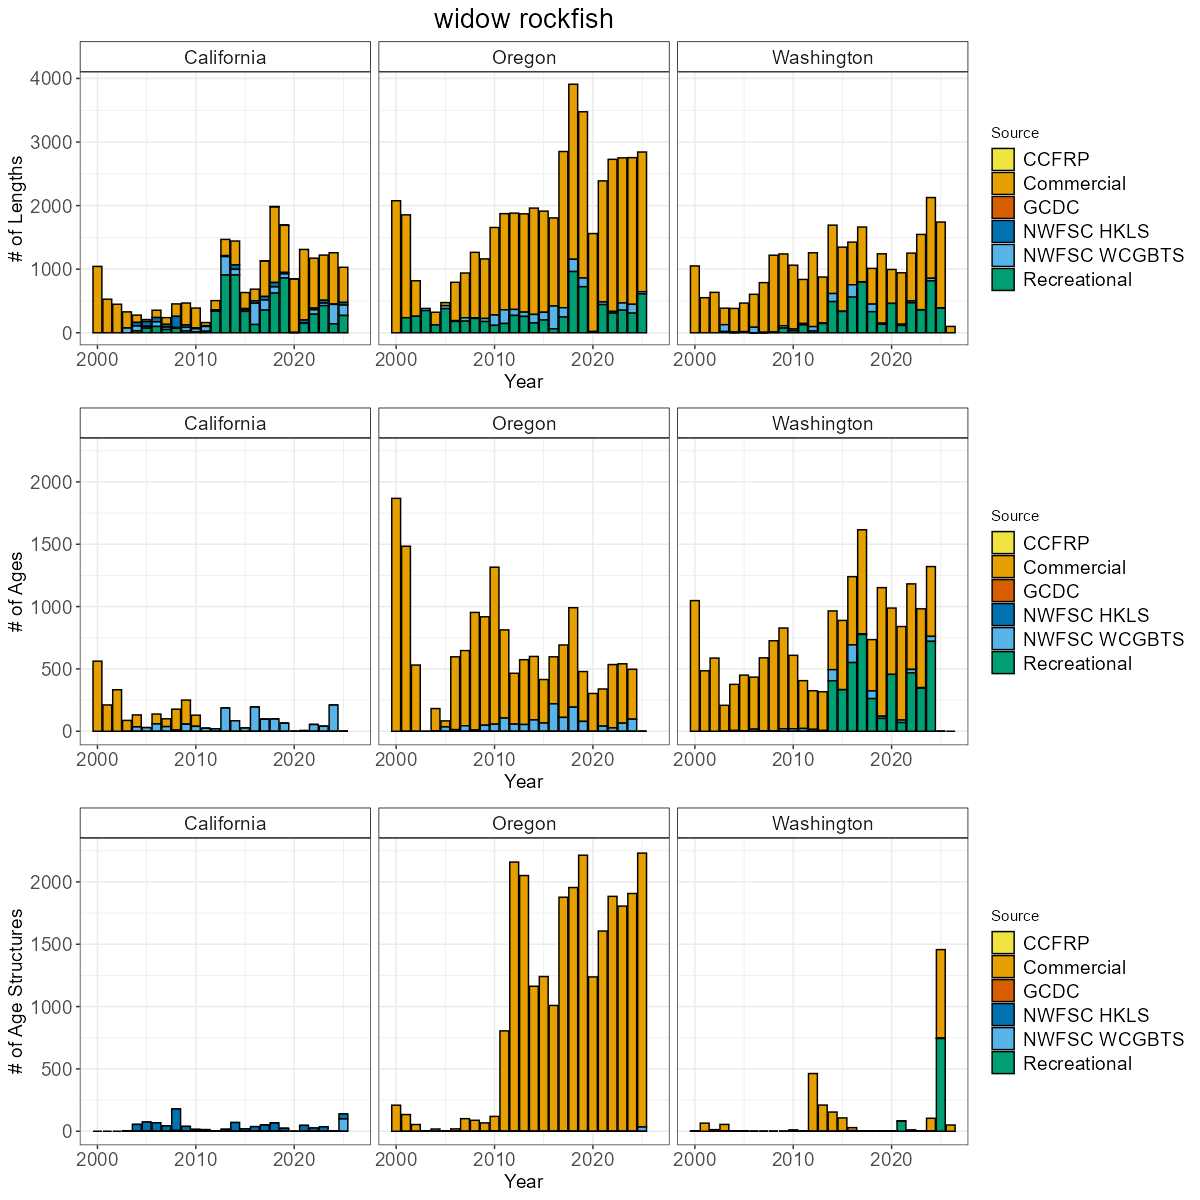
\includegraphics[width=0.95\linewidth,height=\textheight,keepaspectratio]{../plots/state_comparisons/widow_rockfish_state_compositions.png}

}

\caption{Total number of available lengths, read ages, and unread age
structures by data source by year for widow rockfish. Note the y-axis
maximum may differ by data type.}

\end{figure}%

\begin{figure}[H]

{\centering 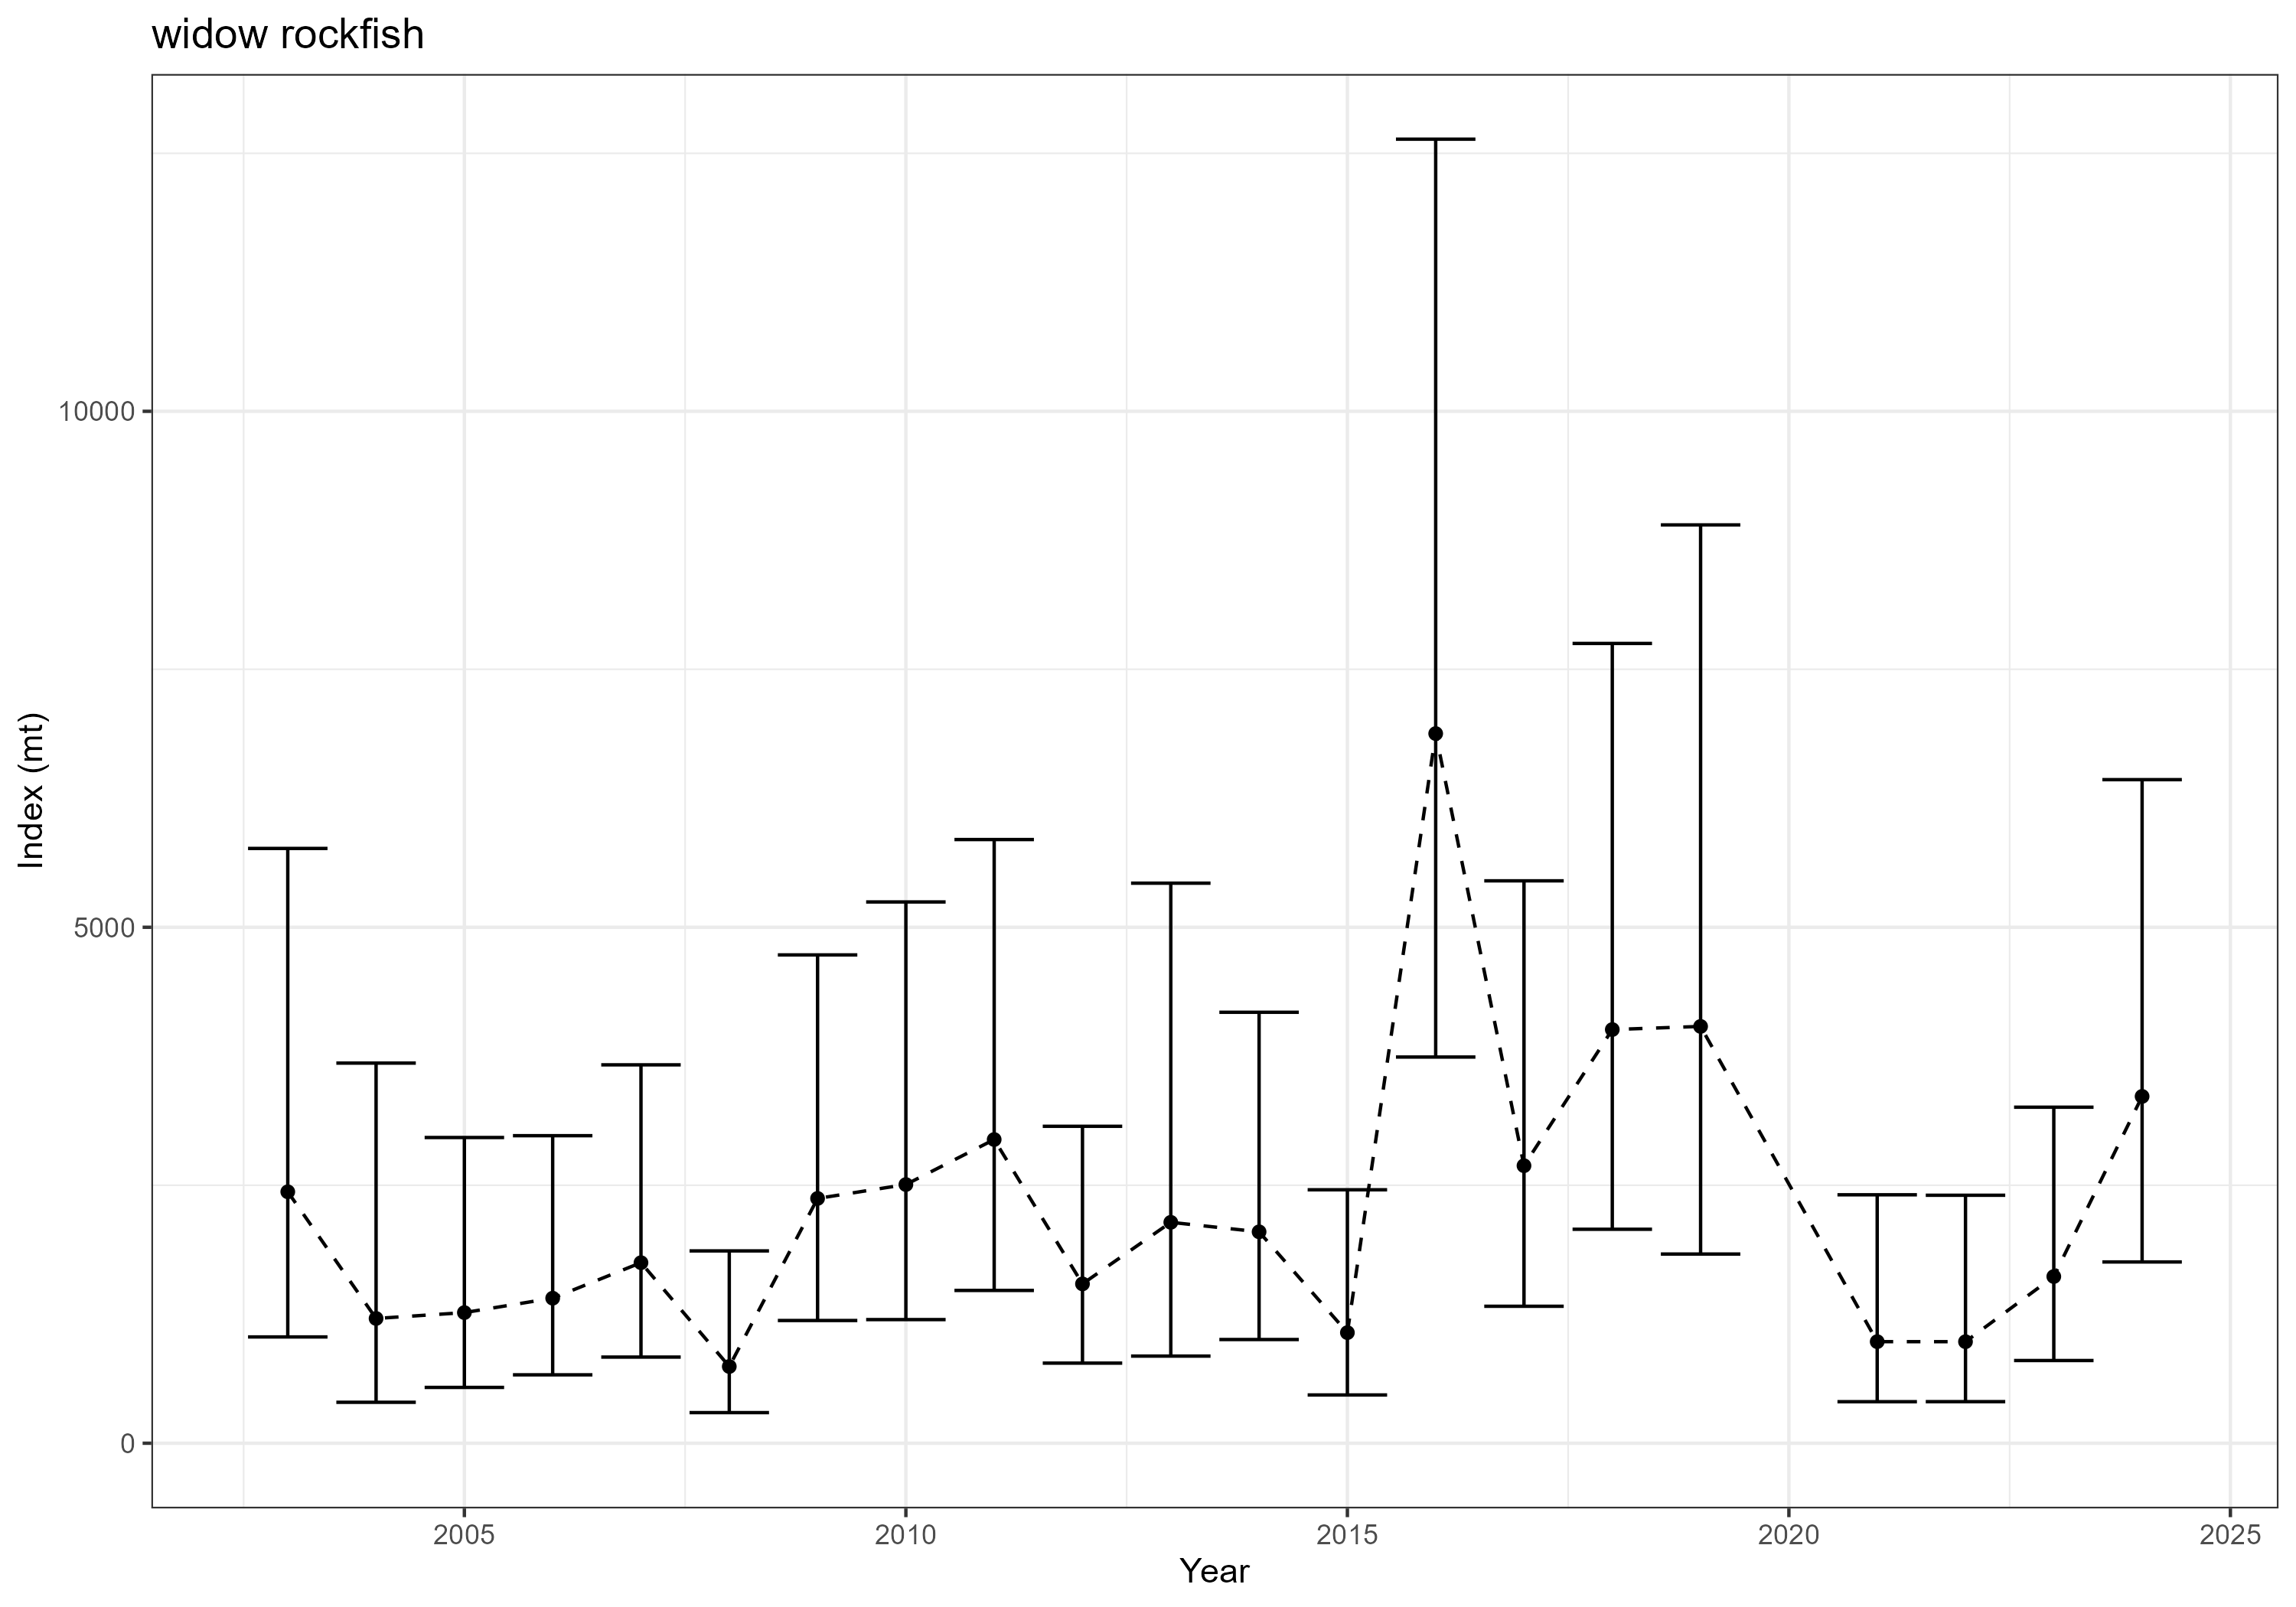
\includegraphics[width=0.95\linewidth,height=\textheight,keepaspectratio]{../plots/wcgbts_indices/widow_rockfish_index.png}

}

\caption{Estimated relative index of abundance for widow rockfish from
the NWFSC WCGBTS.}

\end{figure}%

\begin{figure}[H]

{\centering 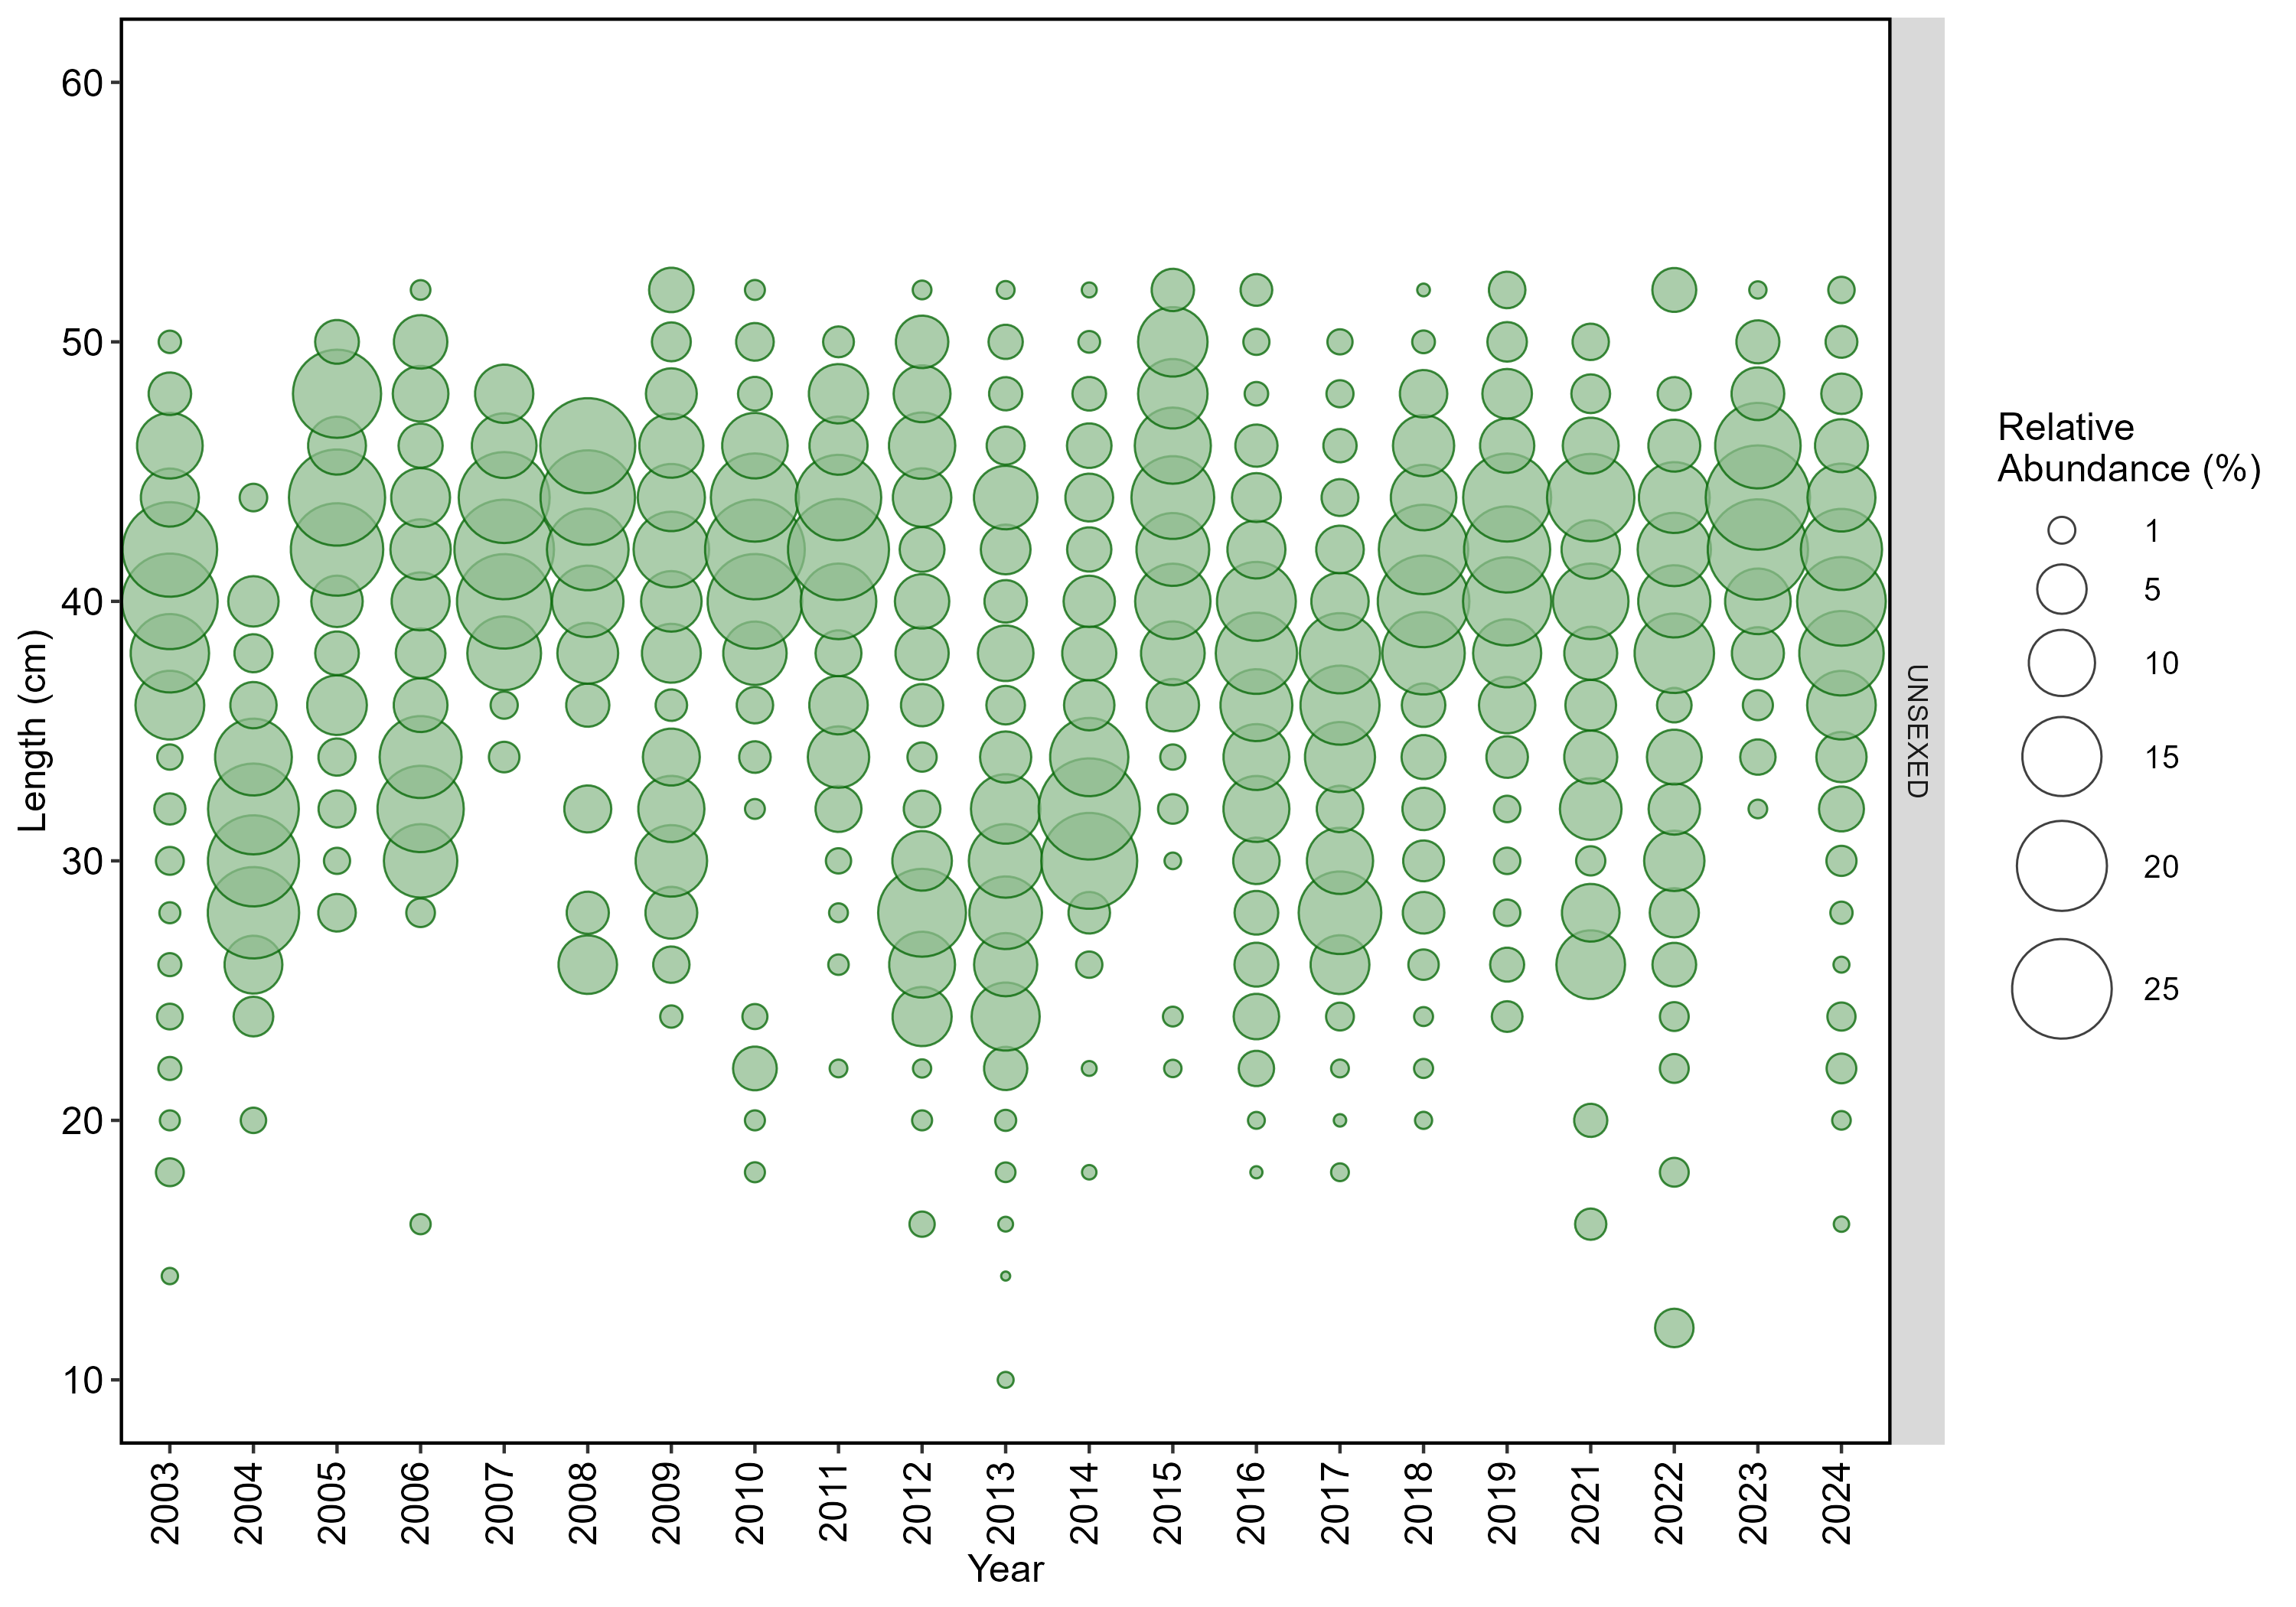
\includegraphics[width=0.95\linewidth,height=\textheight,keepaspectratio]{../plots/wcgbts_comps/plots/widow rockfish_length_frequency_sex_0.png}

}

\caption{Length (cm) compostion data from the NWFSC WCGBTS for widow
rockfish. Size of the circles within a year indicate higher (larger
circles) and lower (smaller circles) proportion observed by length bin.}

\end{figure}%

\begin{figure}[H]

{\centering 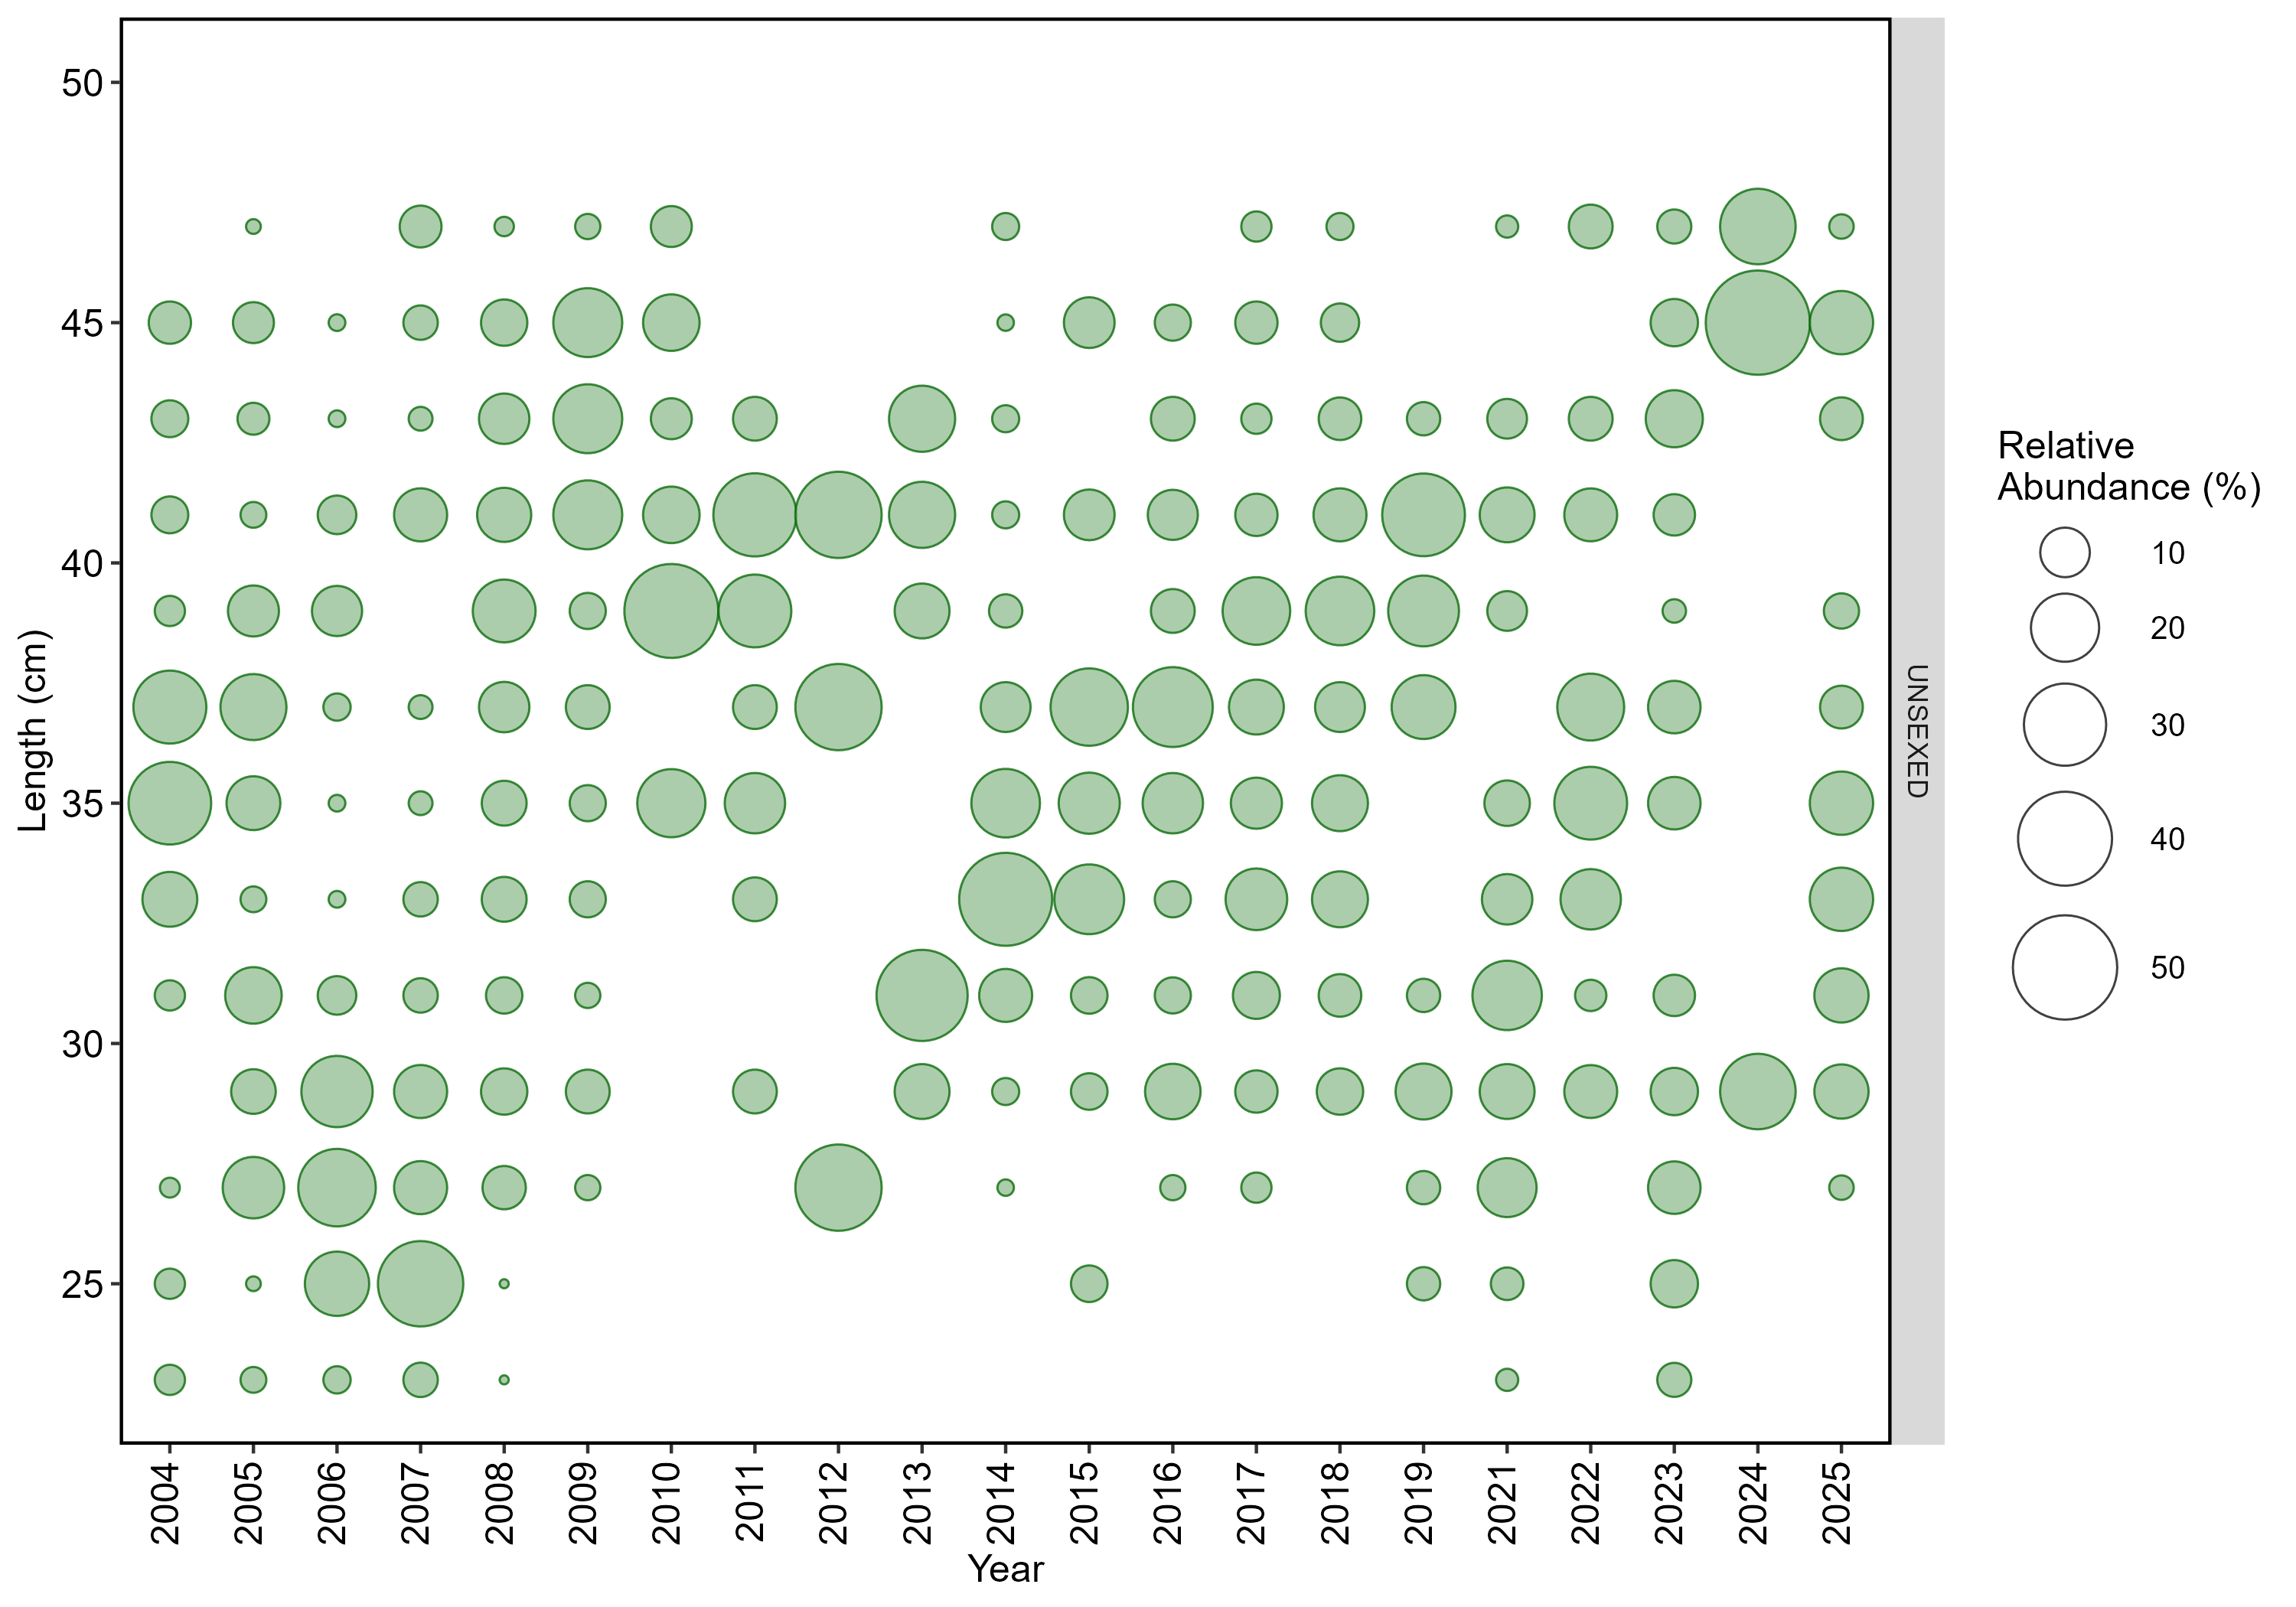
\includegraphics[width=0.95\linewidth,height=\textheight,keepaspectratio]{../plots/hkl_comps/plots/widow rockfish_nwfsc_hkl_length_frequency_sex_0.png}

}

\caption{Length (cm) compostion data from the NWFSC HKLS for widow
rockfish. Size of the circles within a year indicate higher (larger
circles) and lower (smaller circles) proportion observed by length bin.}

\end{figure}%

\newpage{}

\subsection{Yelloweye rockfish}\label{yelloweye-rockfish}

The most recent assessment of yelloweye rockfish was an update
assessment conducted in 2025. Across available data, yelloweye rockfish
have been observed and sampled by both the NWFSC HKLS and WCGBTS. The
NWFSC HKLS observed yelloweye rockfish at an average of 5 sets per year.
The NWFSC WCGBTS observed yelloweye rockfish on an average of 16 tows
per year. For this species, a total of 708 maturity samples have been
collected coastwide (regardless of stock area), with 119 read
maturities.

\begingroup\fontsize{10}{12}\selectfont
\begingroup\fontsize{10}{12}\selectfont

\begin{longtable}[t]{>{\raggedleft\arraybackslash}p{2cm}>{\raggedleft\arraybackslash}p{3.5cm}>{\raggedleft\arraybackslash}p{2cm}>{\raggedleft\arraybackslash}p{2cm}>{\raggedleft\arraybackslash}p{2cm}}
\caption{\label{tab:unnamed-chunk-721}Total number of available lengths, read ages, and unread age structures by data source and
state for yelloweye rockfish.}\\
\toprule
State & Source & Lengths & Ages & Age Structures\\
\midrule
\endfirsthead
\caption[]{Total number of available lengths, read ages, and unread age structures by data source and
state for yelloweye rockfish. (\textit{continued)}}\\
\toprule
State & Source & Lengths & Ages & Age Structures\\
\midrule
\endhead

\endfoot
\bottomrule
\endlastfoot
CA & NWFSC HKLS & 179 & 0 & 170\\
CA & NWFSC WCGBTS & 187 & 167 & 20\\
OR & NWFSC WCGBTS & 474 & 457 & 16\\
WA & NWFSC WCGBTS & 428 & 410 & 18\\*
\end{longtable}
\endgroup{}
\endgroup{}

\begin{figure}[H]

{\centering 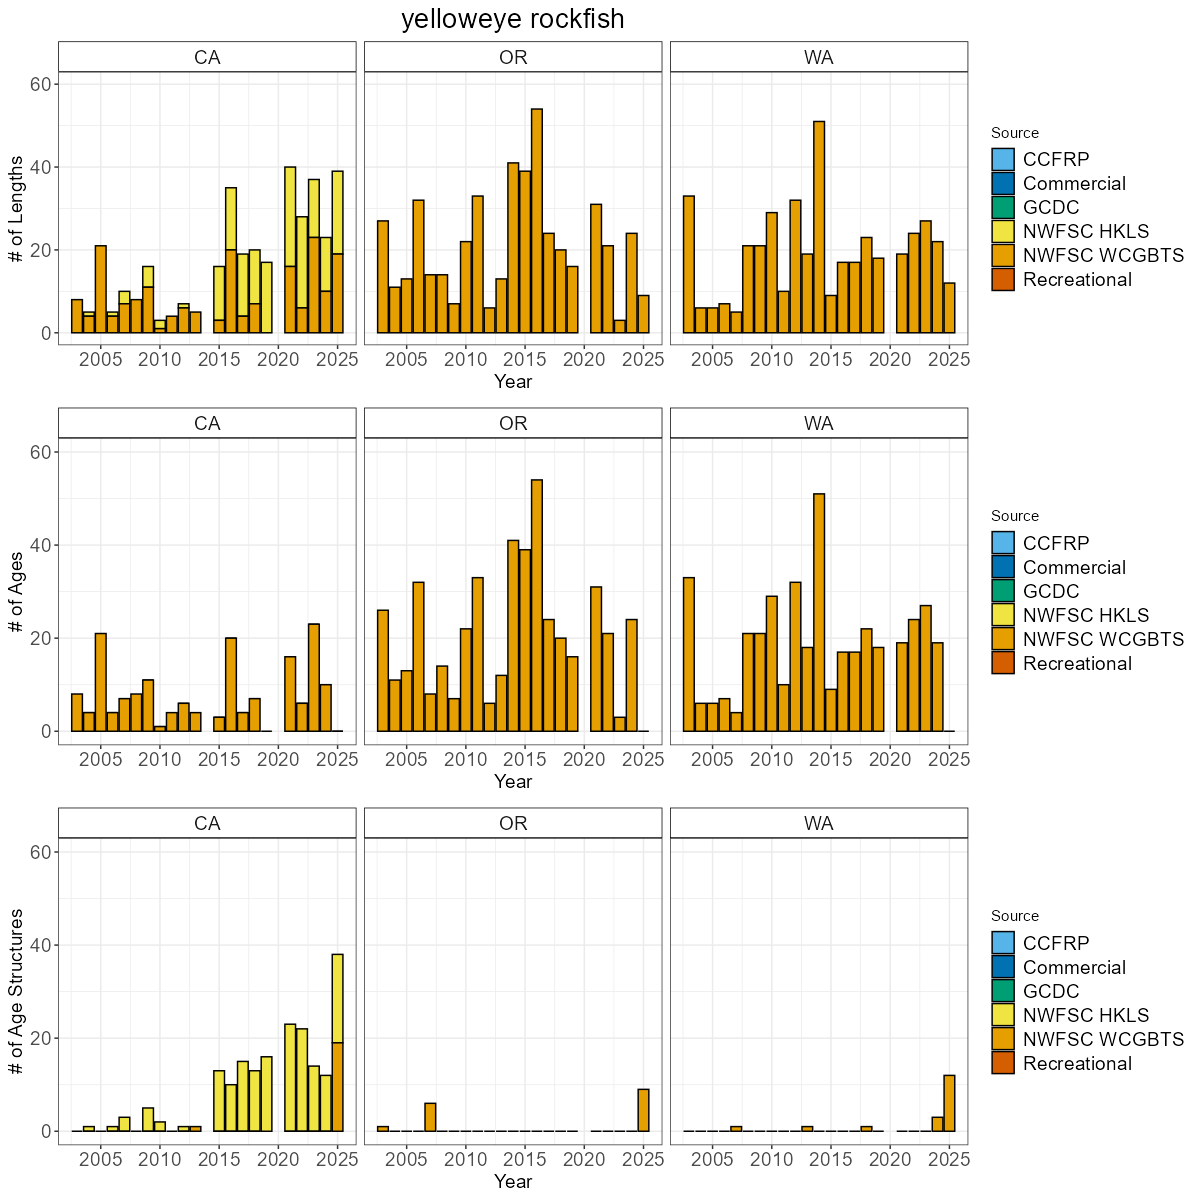
\includegraphics[width=0.95\linewidth,height=\textheight,keepaspectratio]{../plots/state_comparisons/yelloweye_rockfish_state_compositions.png}

}

\caption{Total number of available lengths, read ages, and unread age
structures by data source by year for yelloweye rockfish. Note the
y-axis maximum may differ by data type.}

\end{figure}%

\begin{figure}[H]

{\centering 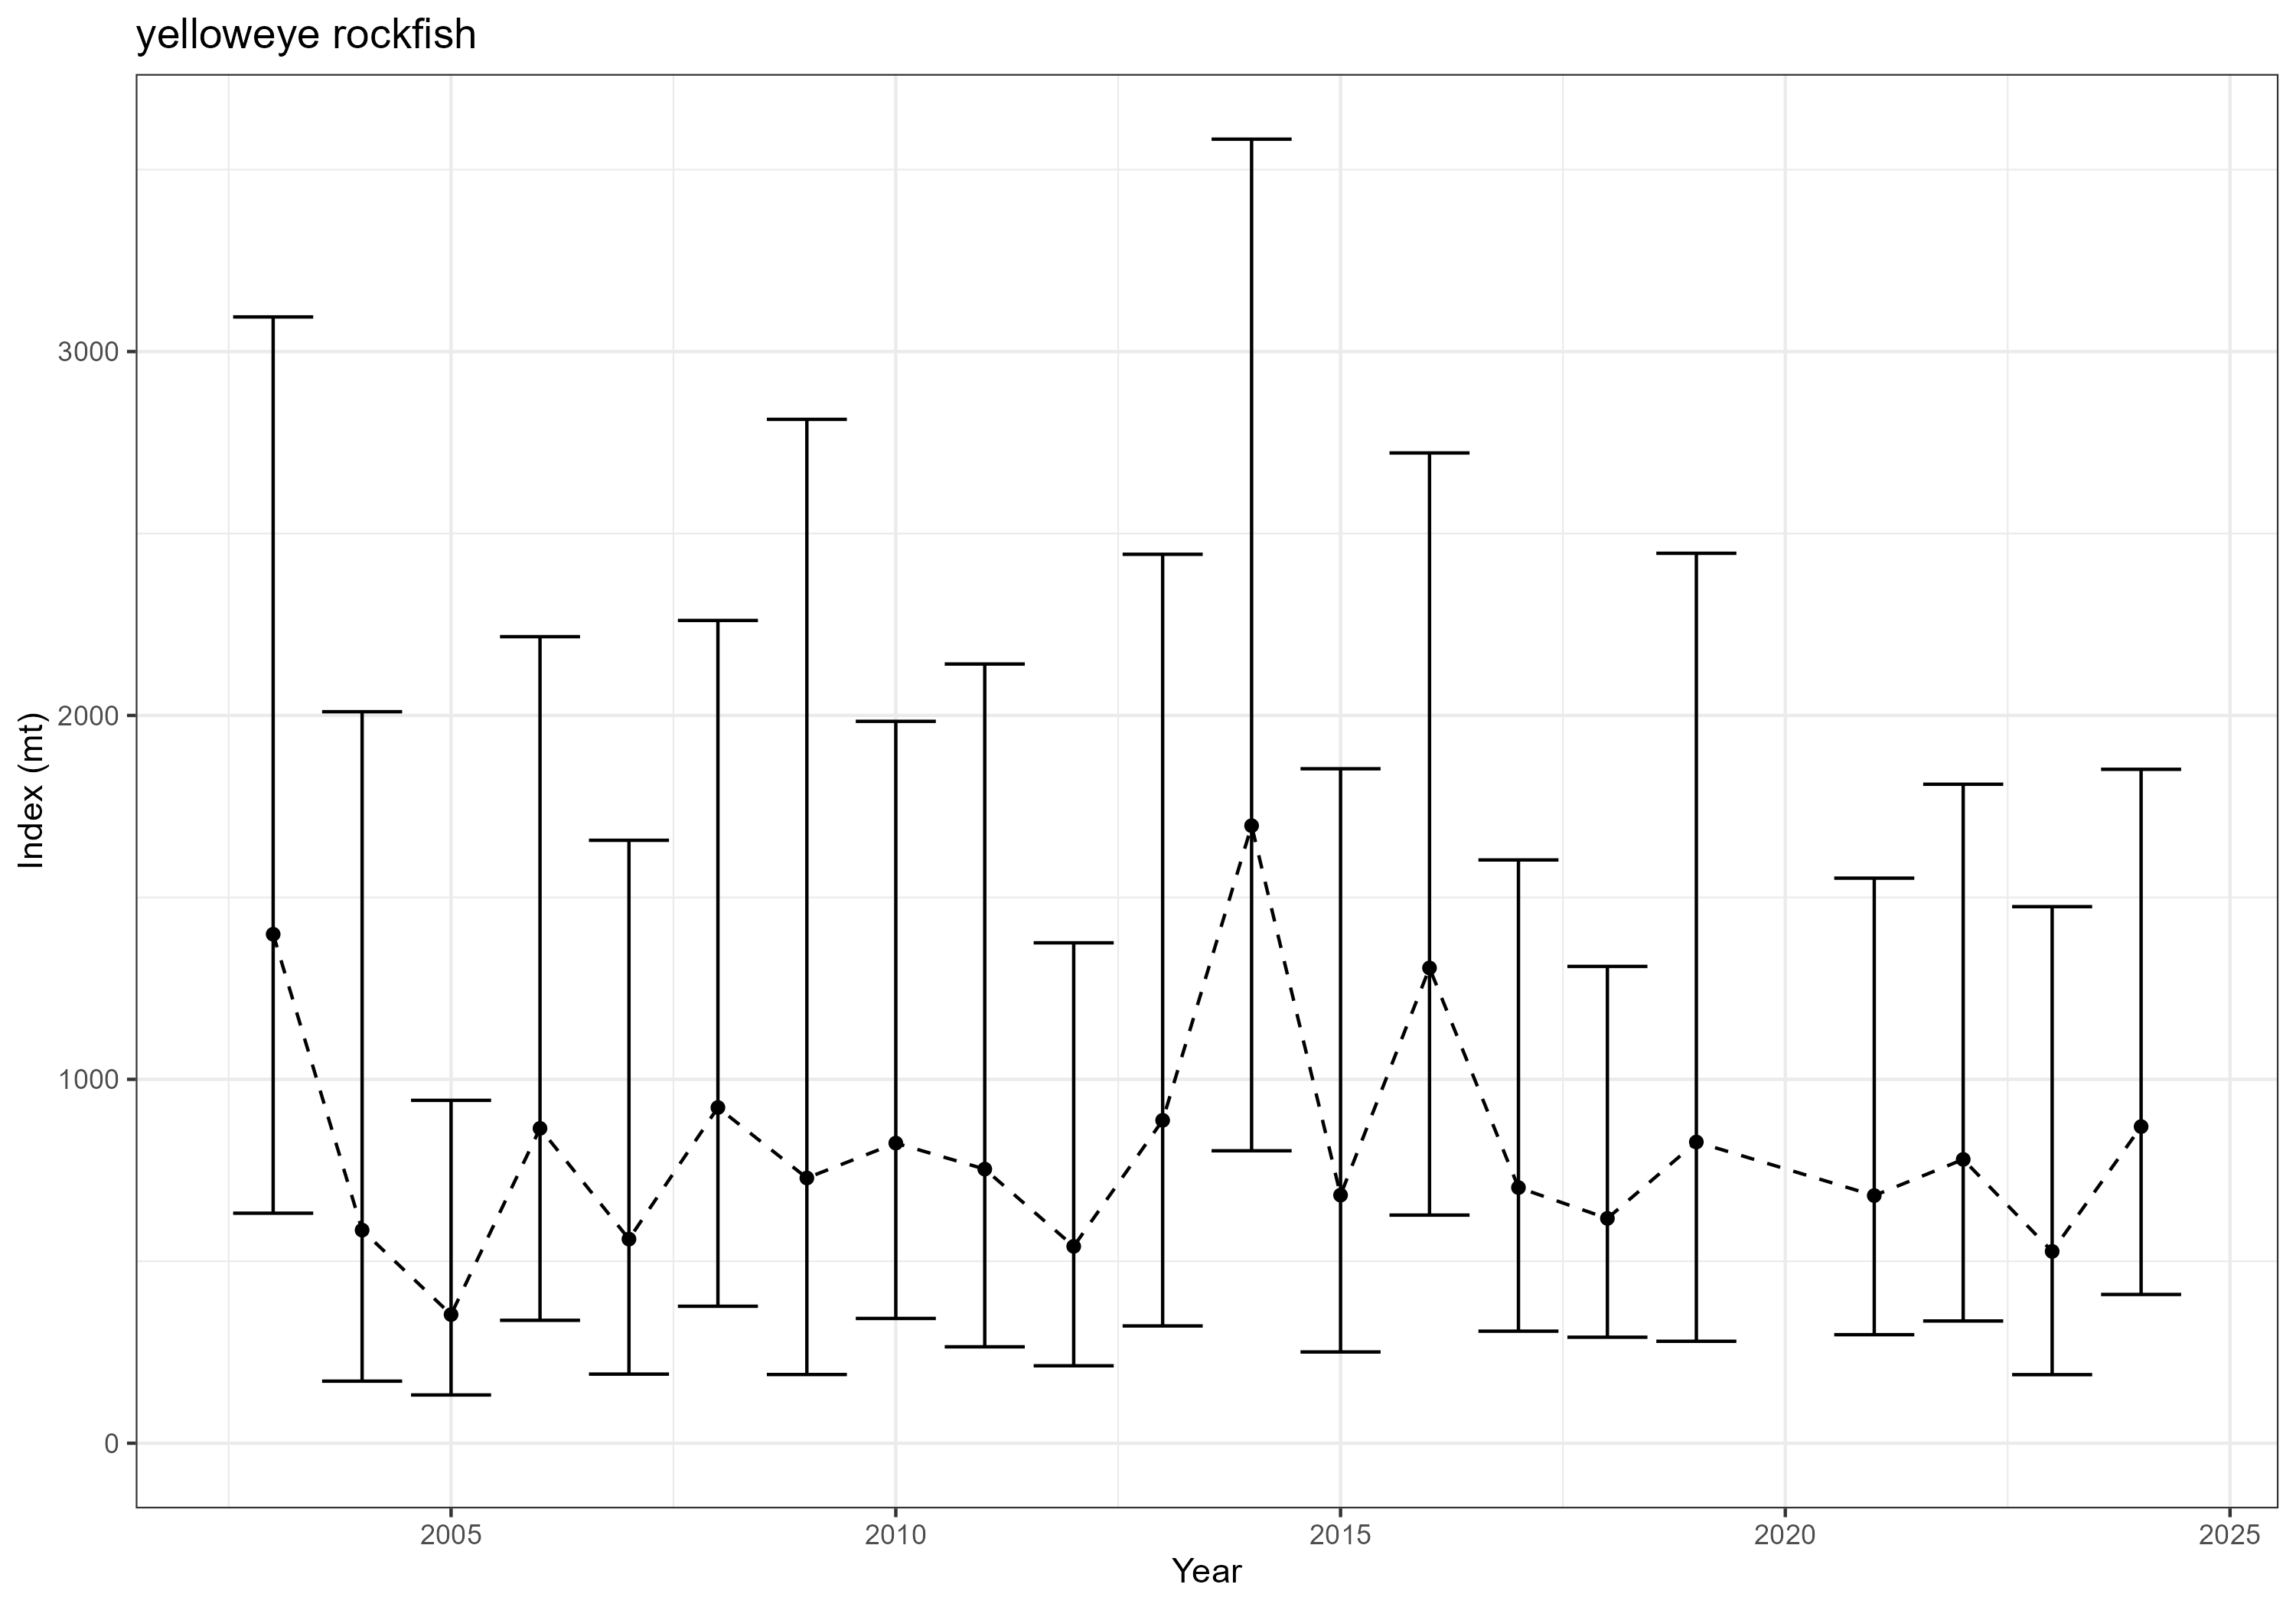
\includegraphics[width=0.95\linewidth,height=\textheight,keepaspectratio]{../plots/wcgbts_indices/yelloweye_rockfish_index.png}

}

\caption{Estimated relative index of abundance for yelloweye rockfish
from the NWFSC WCGBTS.}

\end{figure}%

\begin{figure}[H]

{\centering 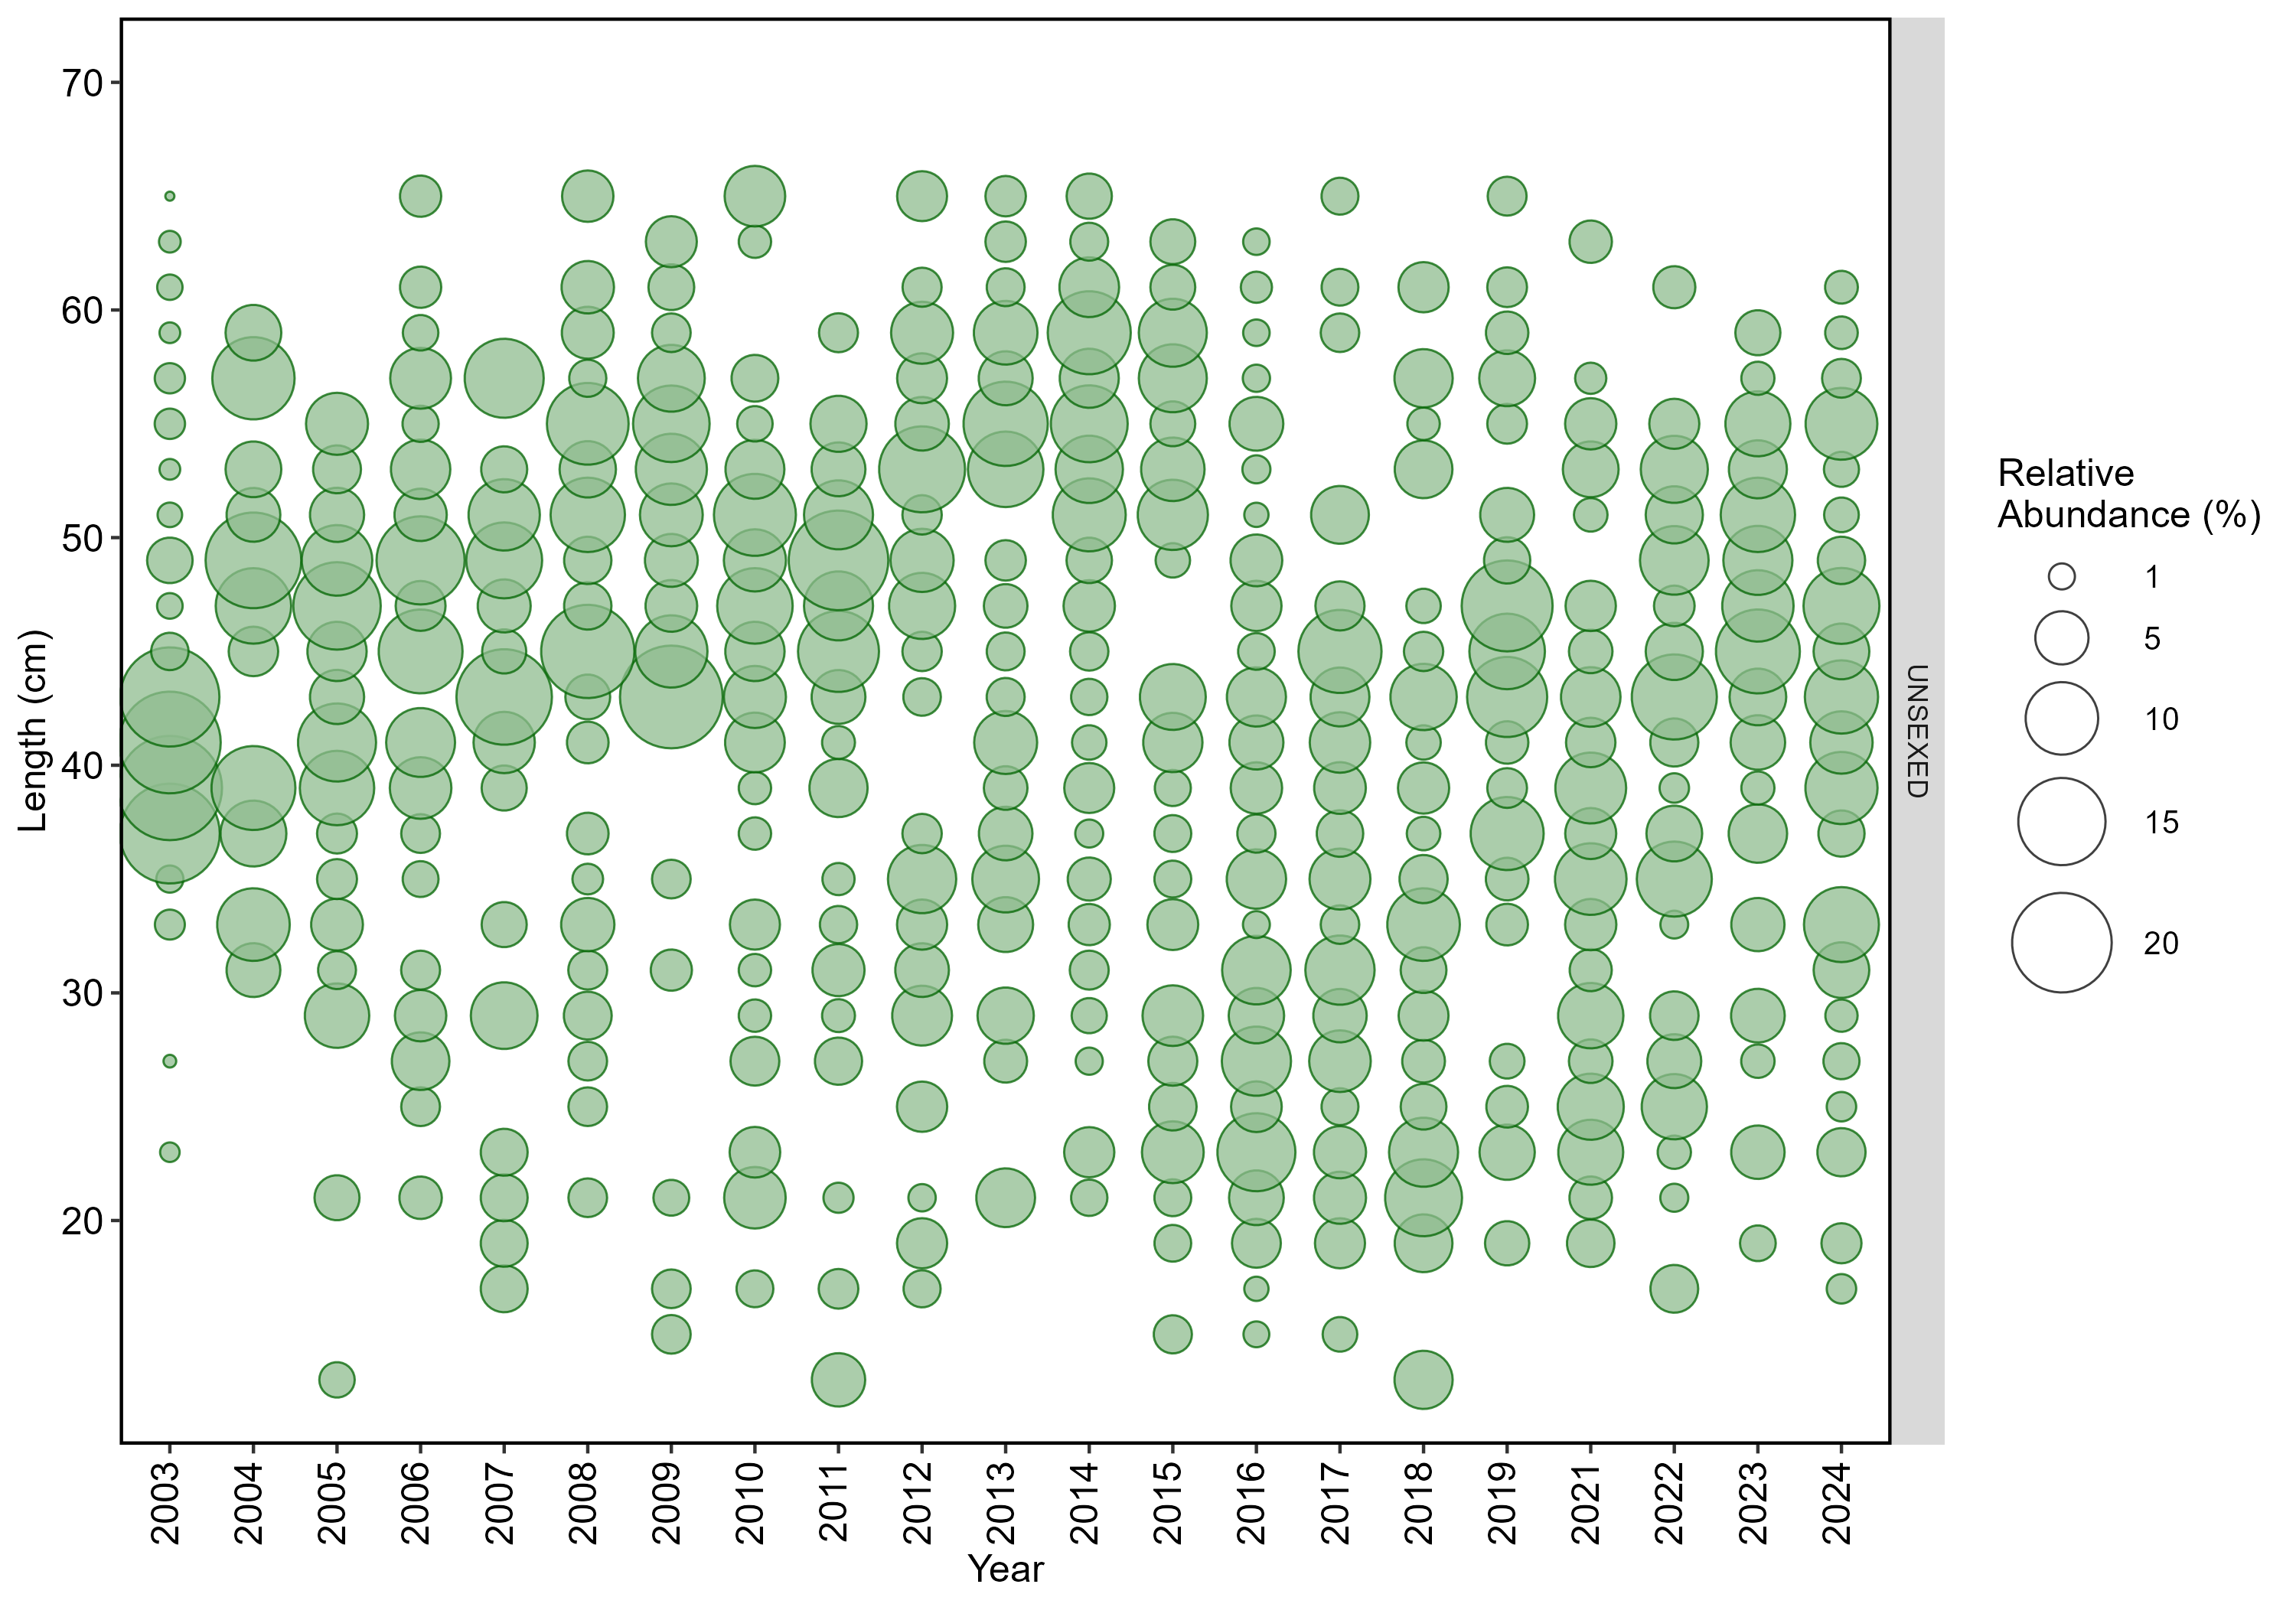
\includegraphics[width=0.95\linewidth,height=\textheight,keepaspectratio]{../plots/wcgbts_comps/plots/yelloweye rockfish_length_frequency_sex_0.png}

}

\caption{Length (cm) compostion data from the NWFSC WCGBTS for yelloweye
rockfish. Size of the circles within a year indicate higher (larger
circles) and lower (smaller circles) proportion observed by length bin.}

\end{figure}%

\newpage{}

\subsection{Yellowmouth rockfish}\label{yellowmouth-rockfish}

To date, no assessment or analysis has been conducted on yellowmouth
rockfish. Across available data, yellowmouth rockfish have been observed
and sampled by the NWFSC WCGBTS. The NWFSC WCGBTS observed yellowmouth
rockfish on an average of 2 tows per year. For this species, a total of
12 maturity samples have been collected coastwide (regardless of stock
area), with 0 read maturities.

\begingroup\fontsize{10}{12}\selectfont
\begingroup\fontsize{10}{12}\selectfont

\begin{longtable}[t]{>{\raggedleft\arraybackslash}p{2cm}>{\raggedleft\arraybackslash}p{3.5cm}>{\raggedleft\arraybackslash}p{2cm}>{\raggedleft\arraybackslash}p{2cm}>{\raggedleft\arraybackslash}p{2cm}}
\caption{\label{tab:unnamed-chunk-738}Total number of available lengths, read ages, and unread age structures by data source and
state for yellowmouth rockfish.}\\
\toprule
State & Source & Lengths & Ages & Age Structures\\
\midrule
\endfirsthead
\caption[]{Total number of available lengths, read ages, and unread age structures by data source and
state for yellowmouth rockfish. (\textit{continued)}}\\
\toprule
State & Source & Lengths & Ages & Age Structures\\
\midrule
\endhead

\endfoot
\bottomrule
\endlastfoot
CA & NWFSC WCGBTS & 1 & 0 & 1\\
OR & NWFSC WCGBTS & 578 & 0 & 309\\
WA & NWFSC WCGBTS & 95 & 0 & 77\\*
\end{longtable}
\endgroup{}
\endgroup{}

\begin{figure}[H]

{\centering 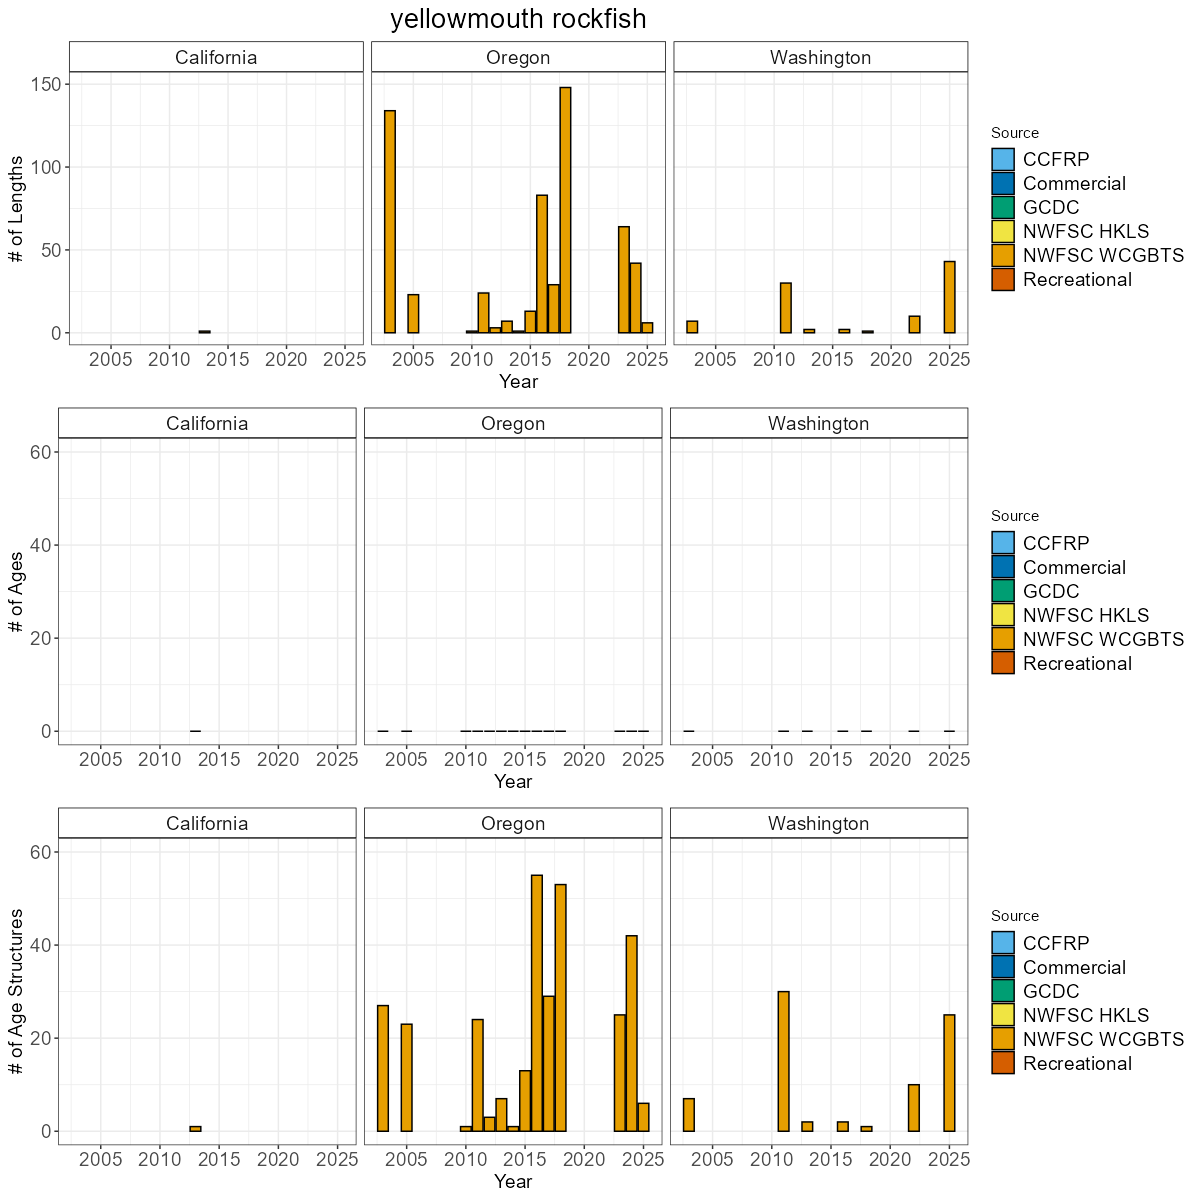
\includegraphics[width=0.95\linewidth,height=\textheight,keepaspectratio]{../plots/state_comparisons/yellowmouth_rockfish_state_compositions.png}

}

\caption{Total number of available lengths, read ages, and unread age
structures by data source by year for yellowmouth rockfish. Note the
y-axis maximum may differ by data type.}

\end{figure}%

\newpage{}

\subsection{Yellowtail rockfish north}\label{yellowtail-rockfish-north}

The most recent assessment of yellowtail rockfish north was a benchmark
assessment conducted in 2025. Across available data, yellowtail rockfish
north have been observed and sampled by the NWFSC WCGBTS. The NWFSC
WCGBTS observed yellowtail rockfish north on an average of 43 tows per
year. For this species, a total of 739 maturity samples have been
collected coastwide (regardless of stock area), with 672 read
maturities. ODFW scientists are planning a research cruise to Cobb Sea
Mount in the summer of 2026 to sample age and sex distributions of this
rockfish species and others.

\begingroup\fontsize{10}{12}\selectfont
\begingroup\fontsize{10}{12}\selectfont

\begin{longtable}[t]{>{\raggedleft\arraybackslash}p{2cm}>{\raggedleft\arraybackslash}p{3.5cm}>{\raggedleft\arraybackslash}p{2cm}>{\raggedleft\arraybackslash}p{2cm}>{\raggedleft\arraybackslash}p{2cm}}
\caption{\label{tab:unnamed-chunk-755}Total number of available lengths, read ages, and unread age structures by data source and
state for yellowtail rockfish north.}\\
\toprule
State & Source & Lengths & Ages & Age Structures\\
\midrule
\endfirsthead
\caption[]{Total number of available lengths, read ages, and unread age structures by data source and
state for yellowtail rockfish north. (\textit{continued)}}\\
\toprule
State & Source & Lengths & Ages & Age Structures\\
\midrule
\endhead

\endfoot
\bottomrule
\endlastfoot
CA & NWFSC WCGBTS & 867 & 292 & 76\\
OR & NWFSC WCGBTS & 3,979 & 1,947 & 446\\
WA & NWFSC WCGBTS & 12,964 & 5,633 & 1,089\\*
\end{longtable}
\endgroup{}
\endgroup{}

\begin{figure}[H]

{\centering 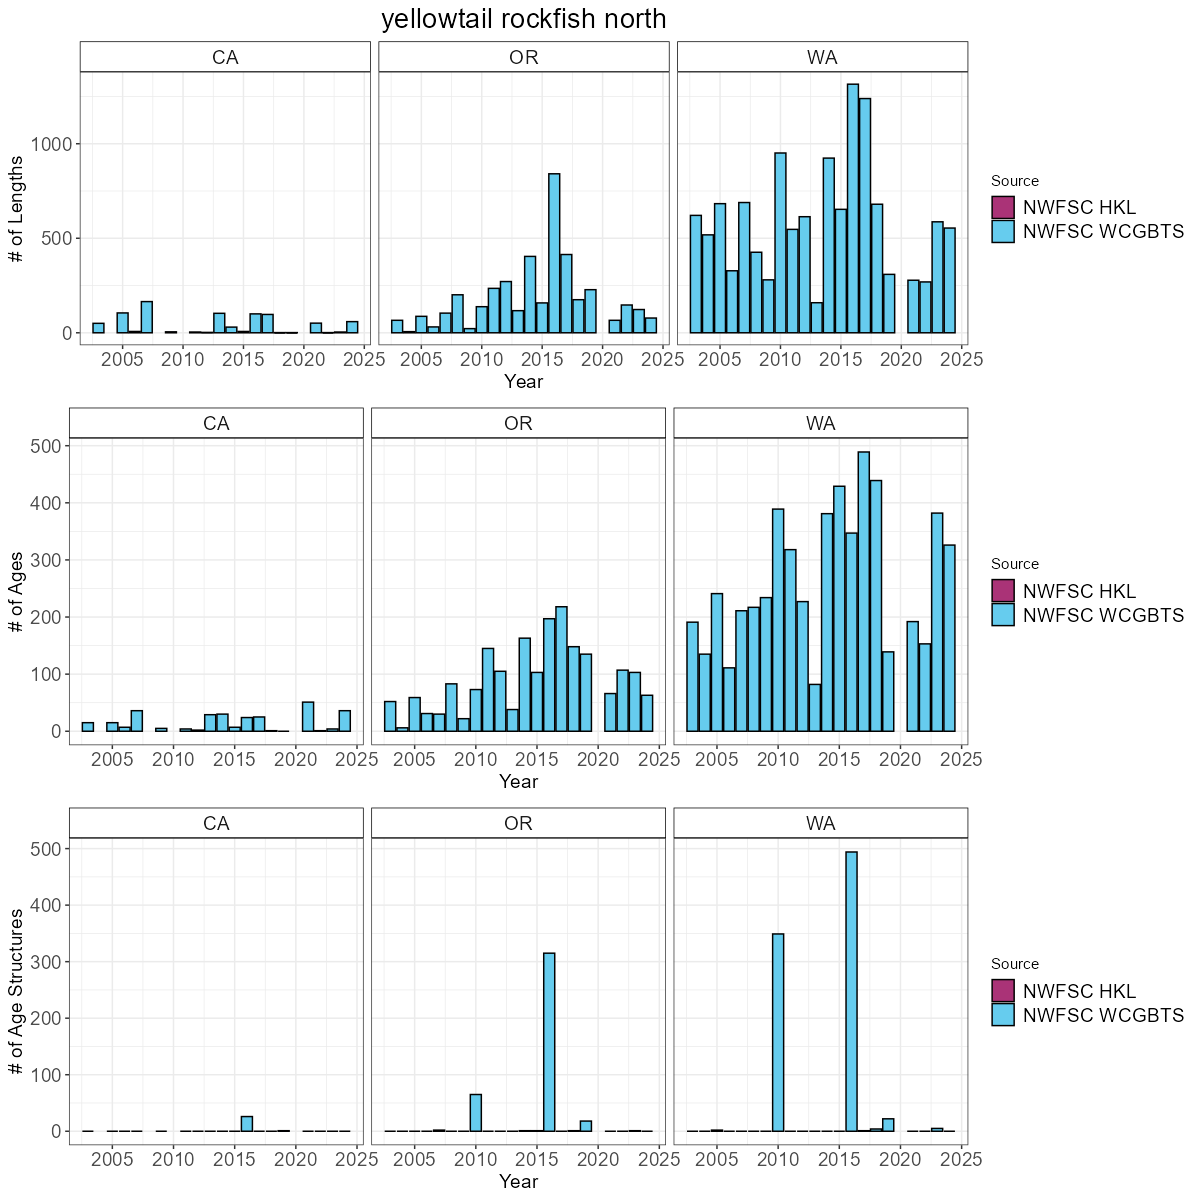
\includegraphics[width=0.95\linewidth,height=\textheight,keepaspectratio]{../plots/state_comparisons/yellowtail_rockfish_north_state_compositions.png}

}

\caption{Total number of available lengths, read ages, and unread age
structures by data source by year for yellowtail rockfish north. Note
the y-axis maximum may differ by data type.}

\end{figure}%

\begin{figure}[H]

{\centering 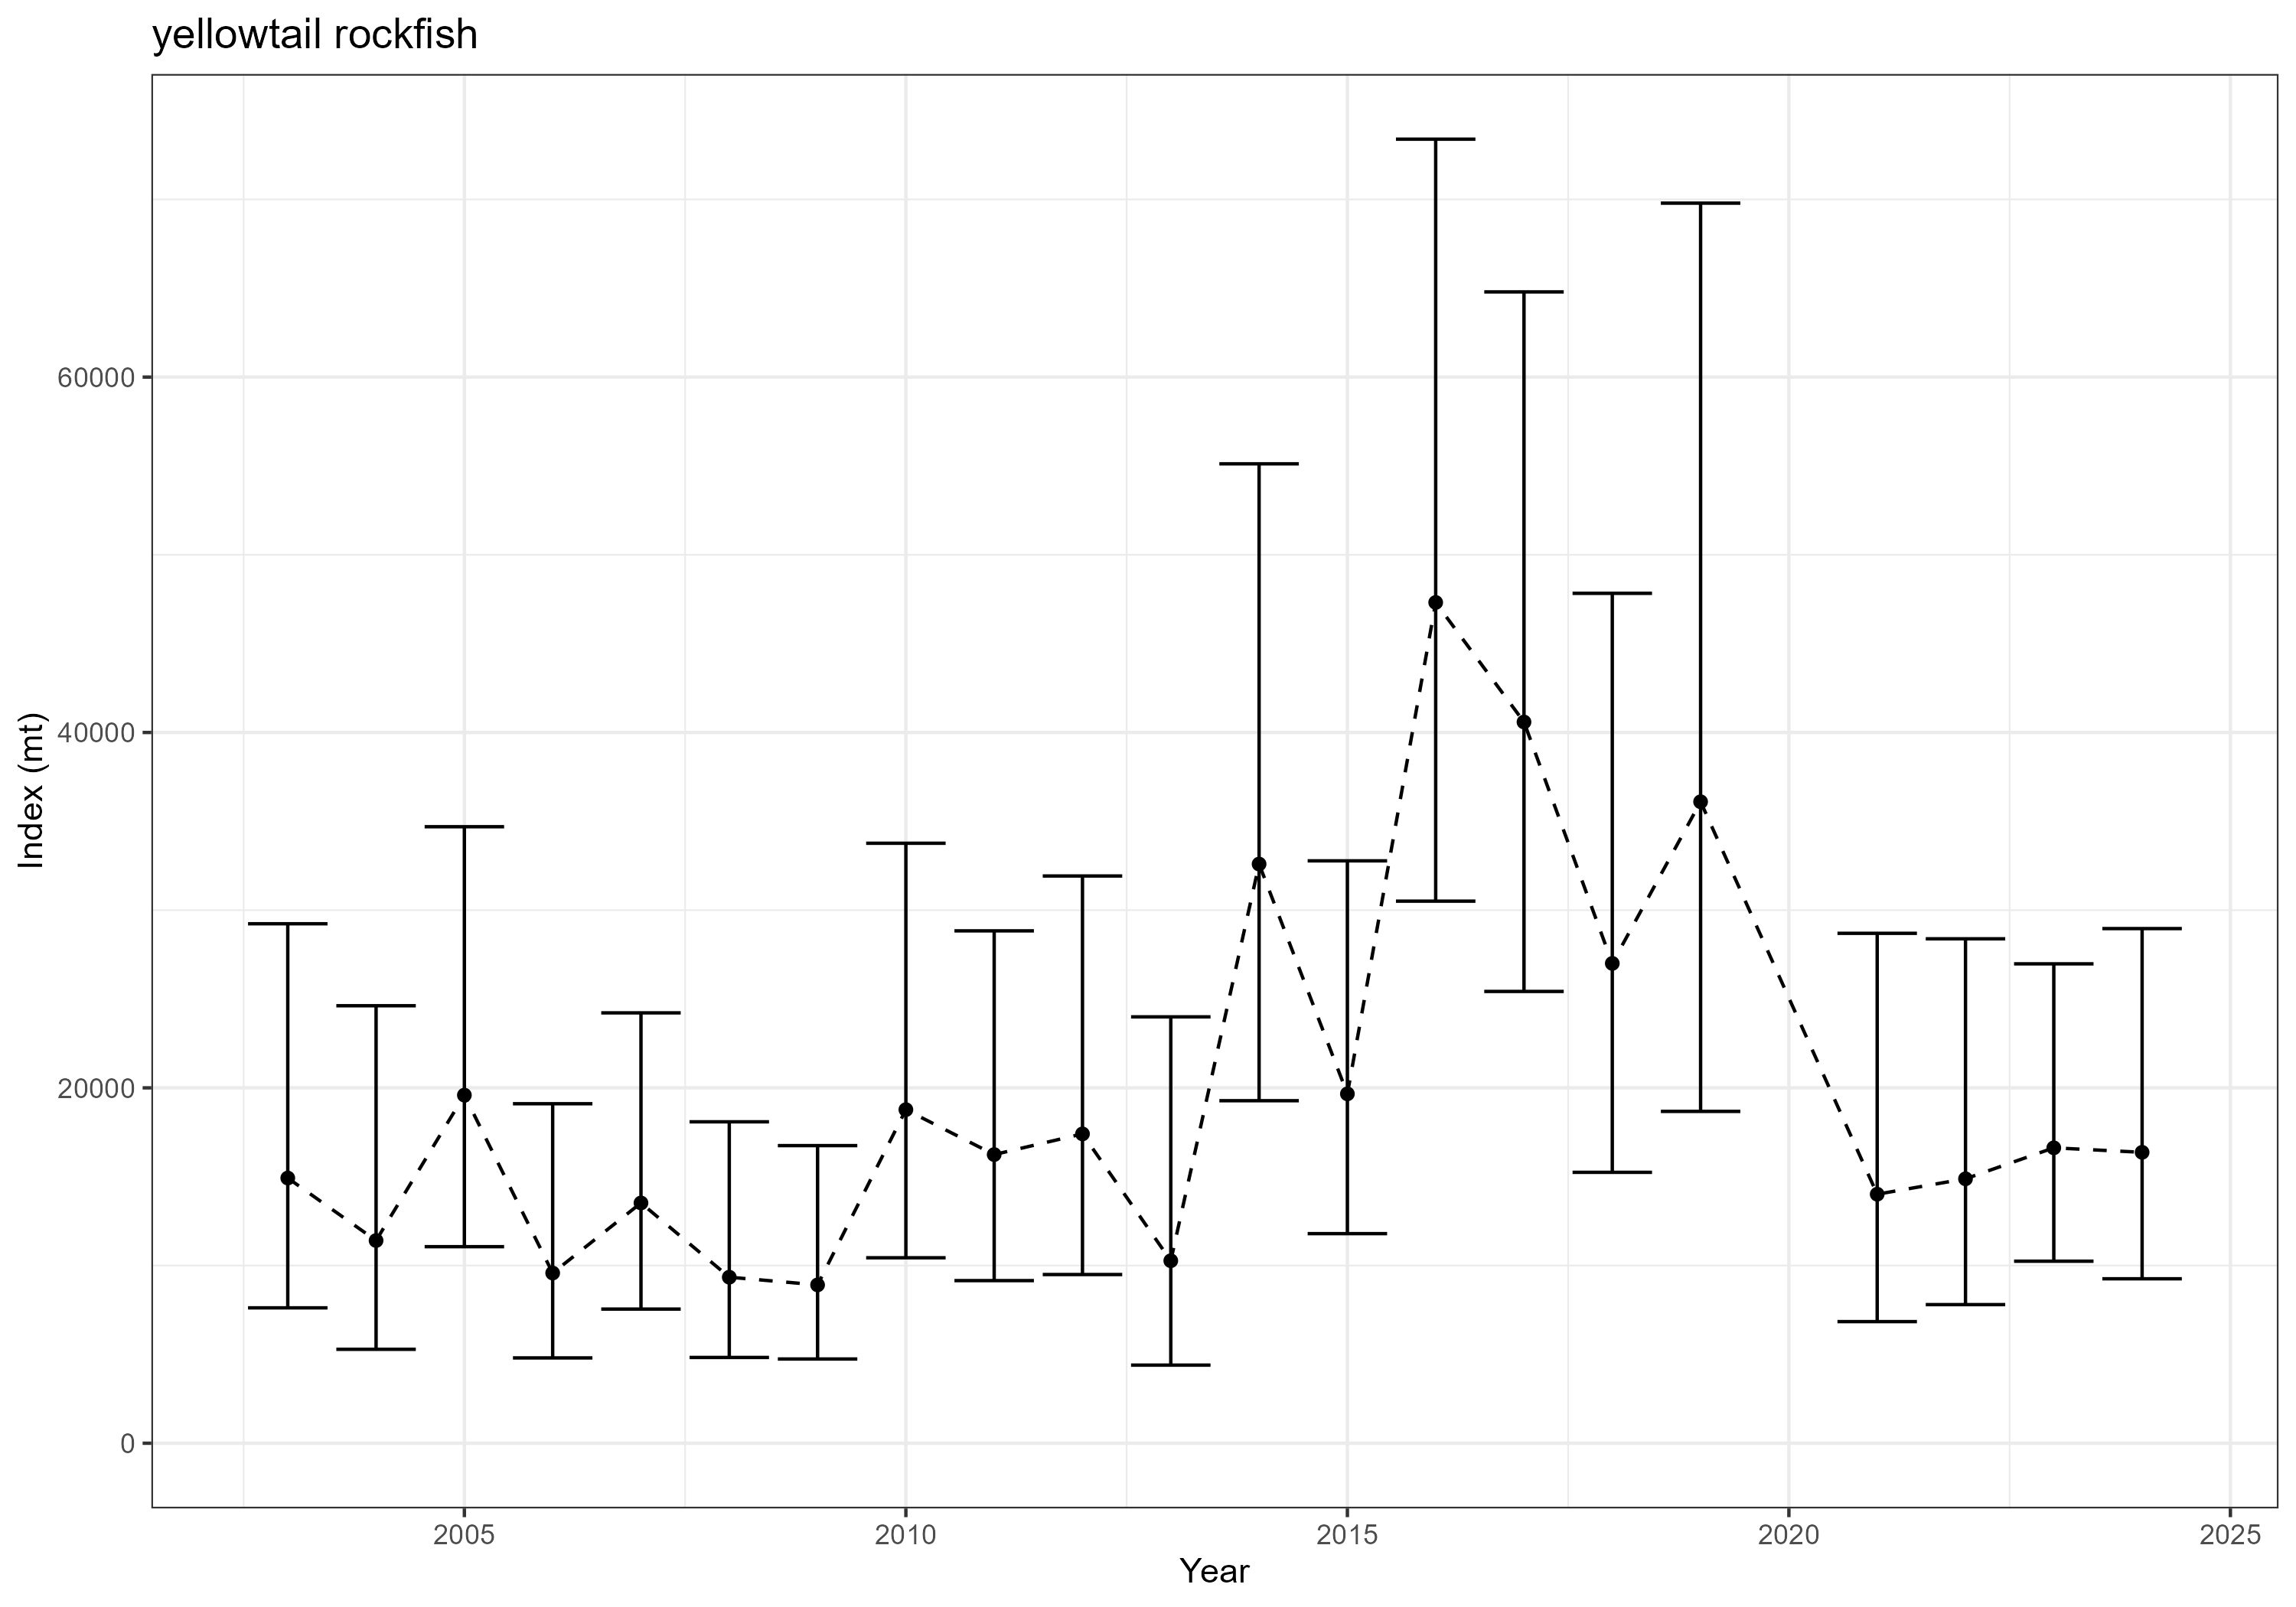
\includegraphics[width=0.95\linewidth,height=\textheight,keepaspectratio]{../plots/wcgbts_indices/yellowtail_rockfish_north_index.png}

}

\caption{Estimated relative index of abundance for yellowtail rockfish
north from the NWFSC WCGBTS.}

\end{figure}%

\begin{figure}[H]

{\centering 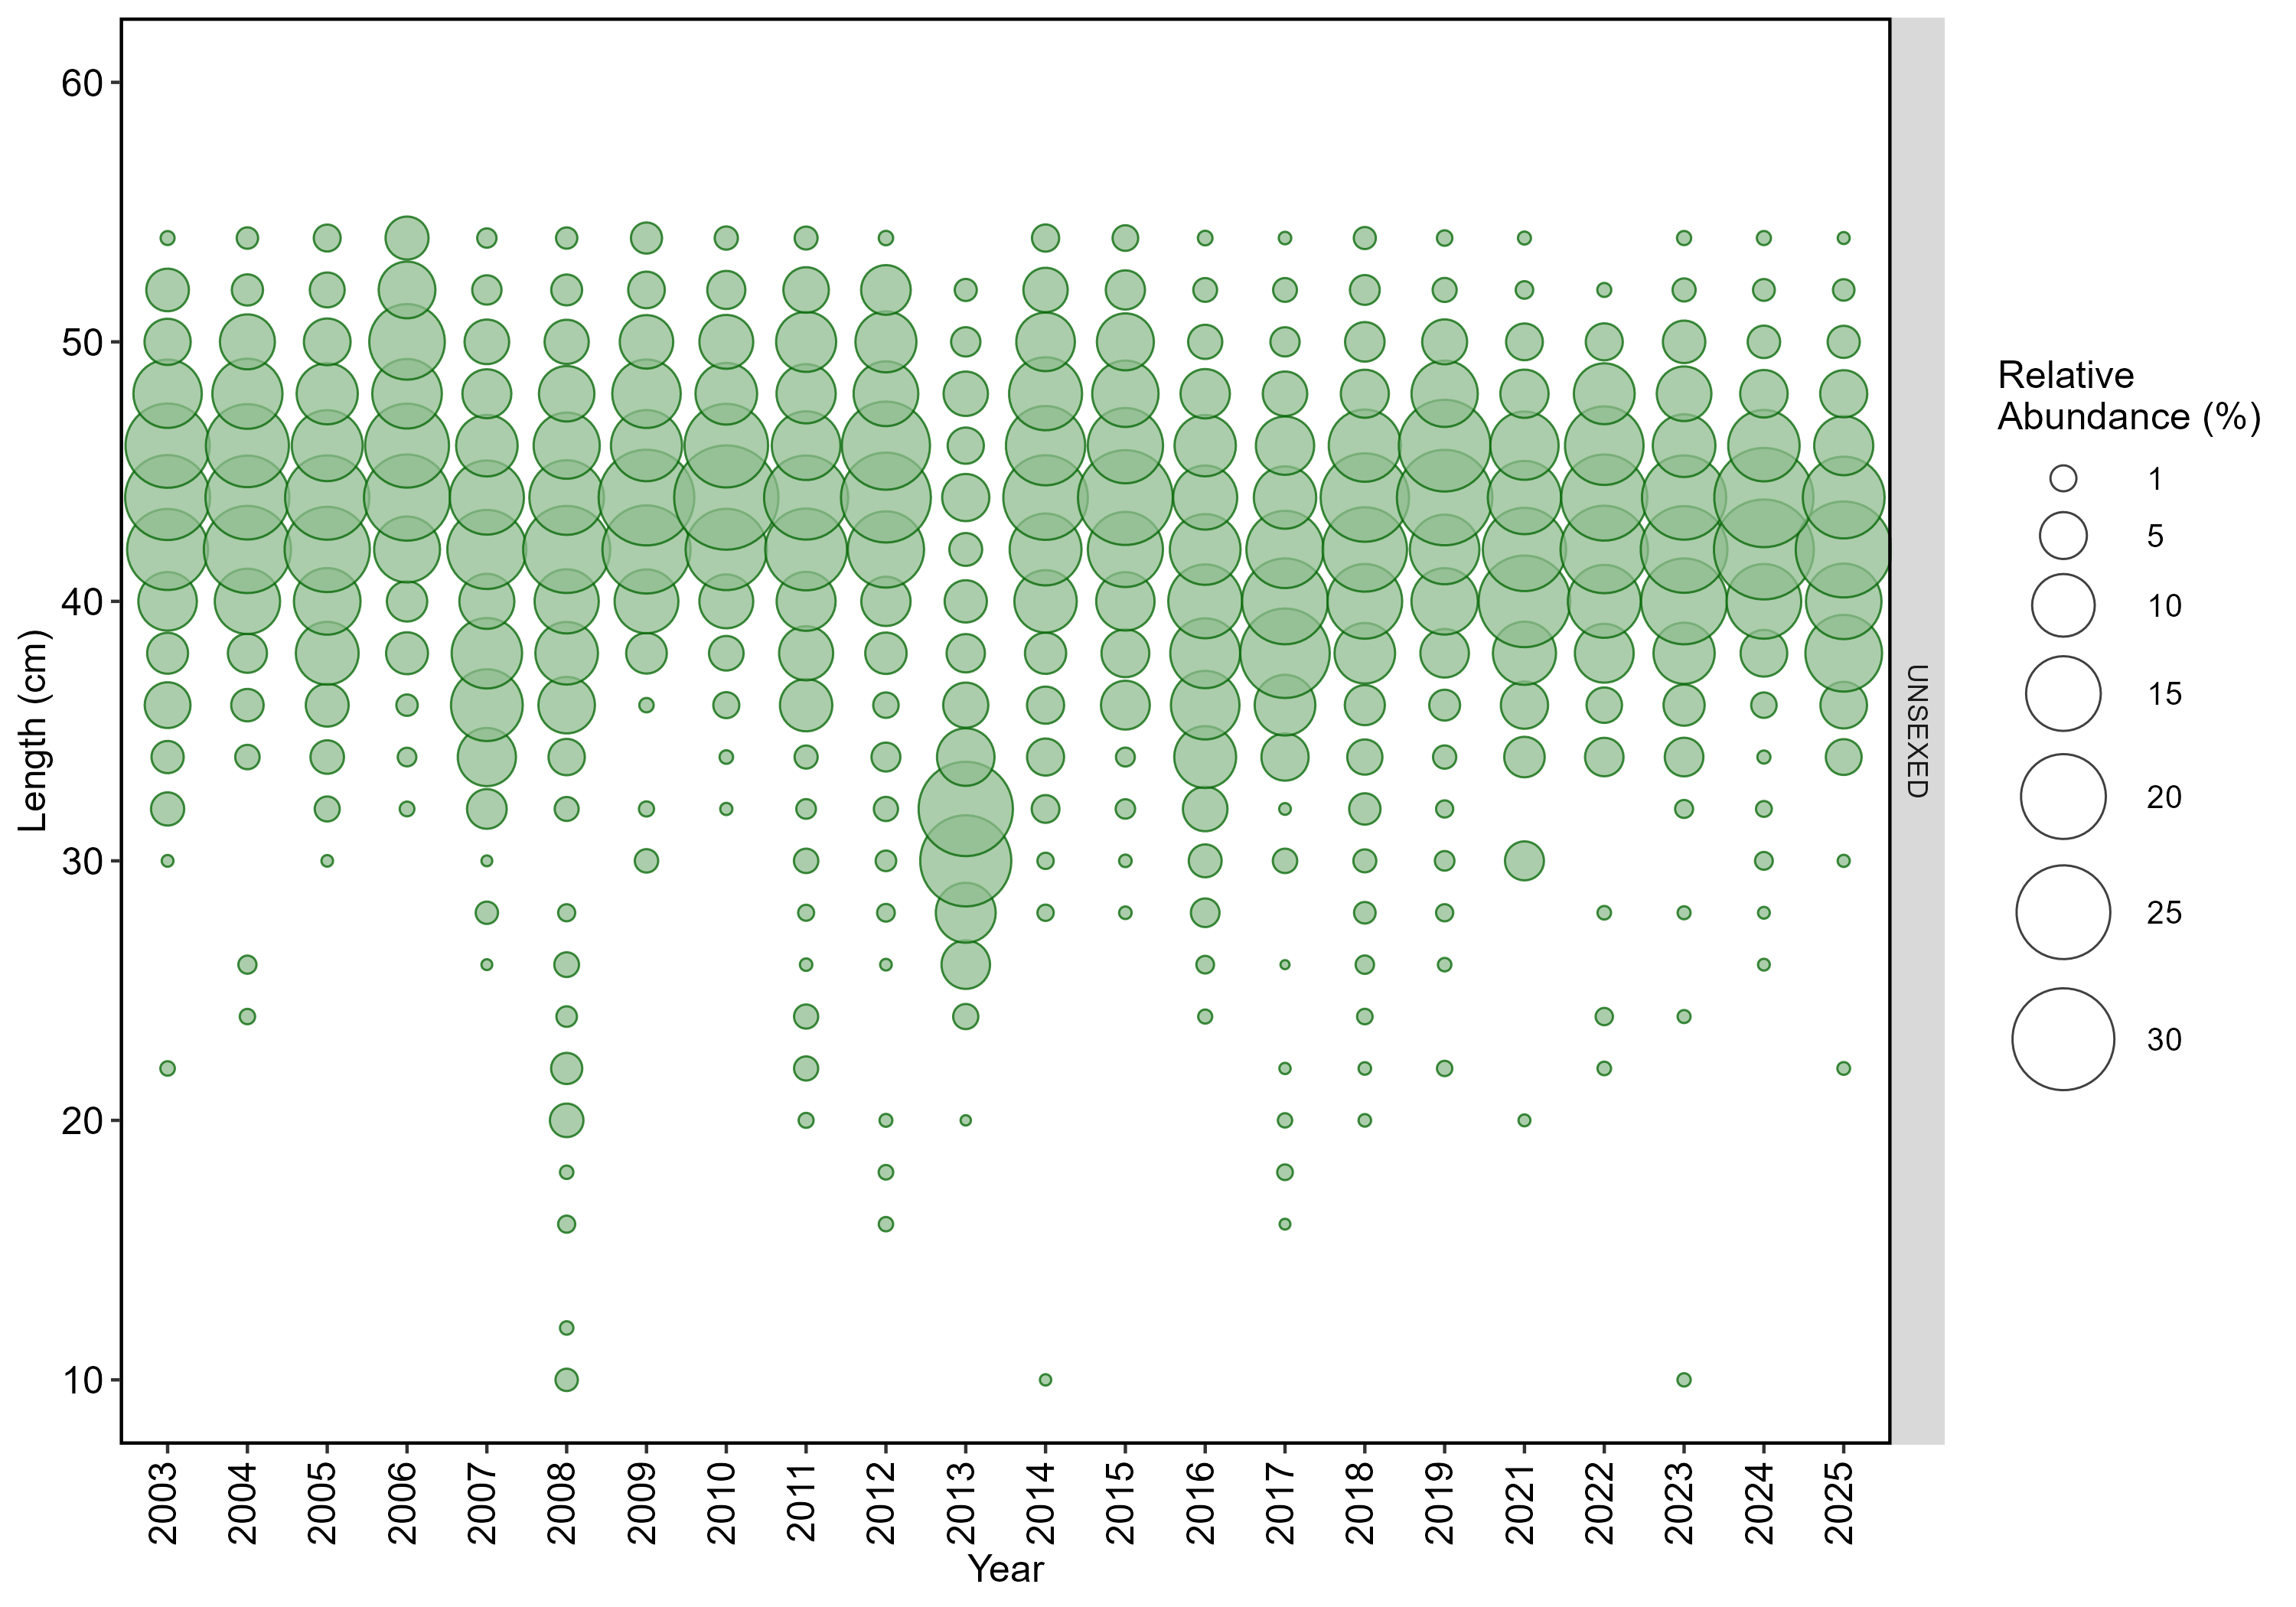
\includegraphics[width=0.95\linewidth,height=\textheight,keepaspectratio]{../plots/wcgbts_comps/plots/yellowtail rockfish north_length_frequency_sex_0.png}

}

\caption{Length (cm) compostion data from the NWFSC WCGBTS for
yellowtail rockfish north. Size of the circles within a year indicate
higher (larger circles) and lower (smaller circles) proportion observed
by length bin.}

\end{figure}%

\newpage{}

\subsection{Yellowtail rockfish south}\label{yellowtail-rockfish-south}

To date, no assessment or analysis has been conducted on yellowtail
rockfish south. Across available data, yellowtail rockfish south have
been observed and sampled by both the NWFSC HKLS and WCGBTS. The NWFSC
HKLS observed yellowtail rockfish south at an average of 13 sets per
year. The NWFSC WCGBTS observed yellowtail rockfish south on an average
of 3 tows per year. For this species, a total of 739 maturity samples
have been collected coastwide (regardless of stock area), with 672 read
maturities.

\begingroup\fontsize{10}{12}\selectfont
\begingroup\fontsize{10}{12}\selectfont

\begin{longtable}[t]{>{\raggedleft\arraybackslash}p{2cm}>{\raggedleft\arraybackslash}p{3.5cm}>{\raggedleft\arraybackslash}p{2cm}>{\raggedleft\arraybackslash}p{2cm}>{\raggedleft\arraybackslash}p{2cm}}
\caption{\label{tab:unnamed-chunk-772}Total number of available lengths, read ages, and unread age structures by data source and
state for yellowtail rockfish south.}\\
\toprule
State & Source & Lengths & Ages & Age Structures\\
\midrule
\endfirsthead
\caption[]{Total number of available lengths, read ages, and unread age structures by data source and
state for yellowtail rockfish south. (\textit{continued)}}\\
\toprule
State & Source & Lengths & Ages & Age Structures\\
\midrule
\endhead

\endfoot
\bottomrule
\endlastfoot
CA & NWFSC HKLS & 2,011 & 124 & 1,666\\
CA & NWFSC WCGBTS & 1,158 & 534 & 77\\*
\end{longtable}
\endgroup{}
\endgroup{}

\begin{figure}[H]

{\centering 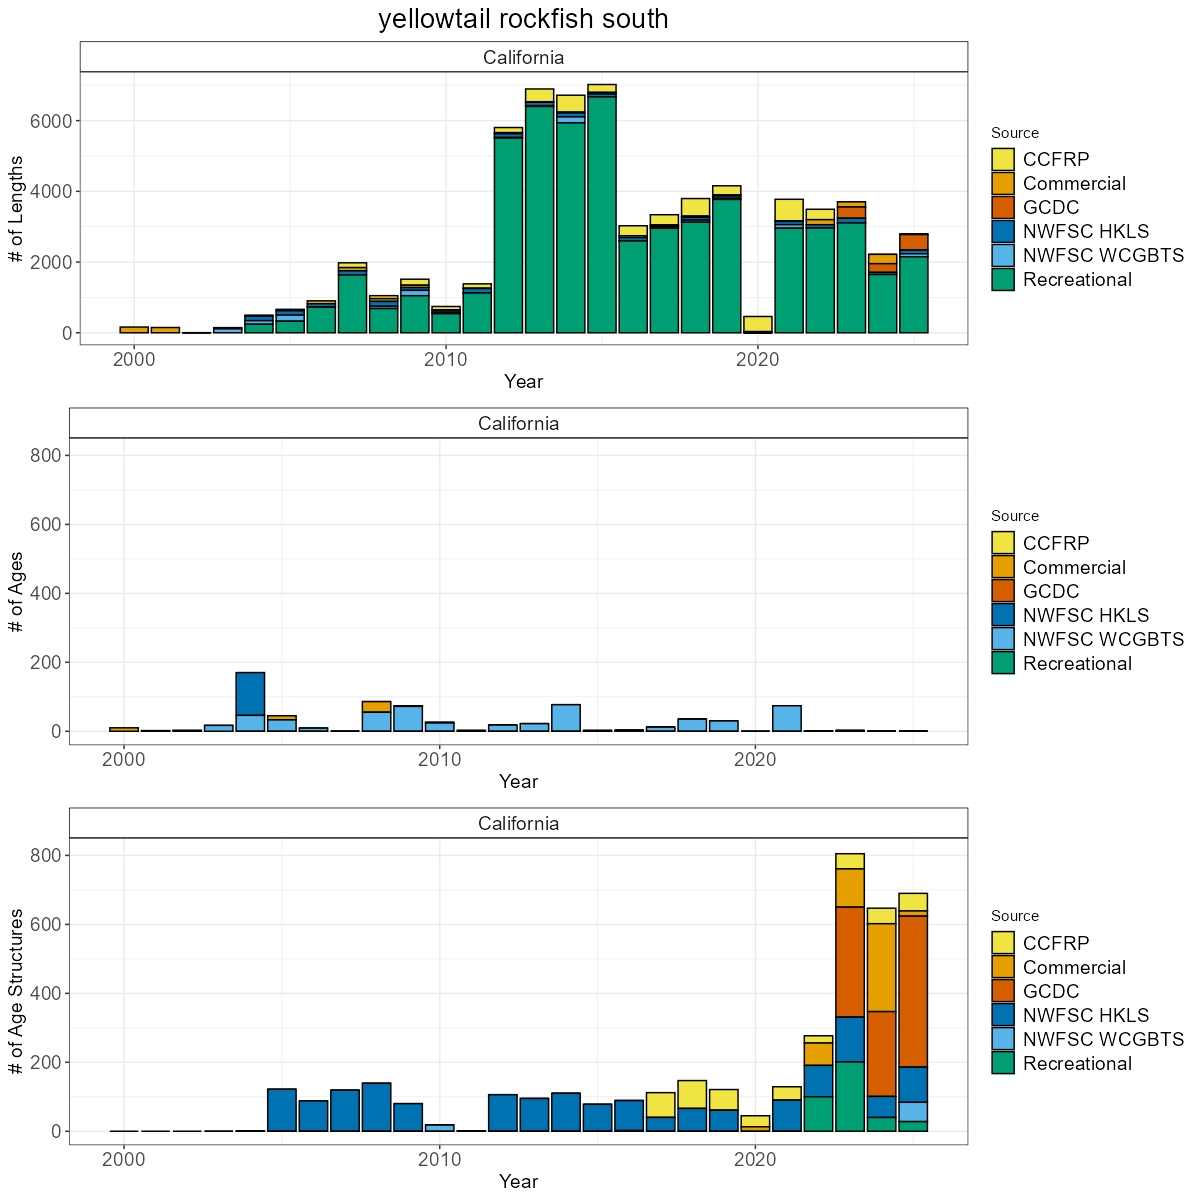
\includegraphics[width=0.95\linewidth,height=\textheight,keepaspectratio]{../plots/state_comparisons/yellowtail_rockfish_south_state_compositions.png}

}

\caption{Total number of available lengths, read ages, and unread age
structures by data source by year for yellowtail rockfish south. Note
the y-axis maximum may differ by data type.}

\end{figure}%

\begin{figure}[H]

{\centering 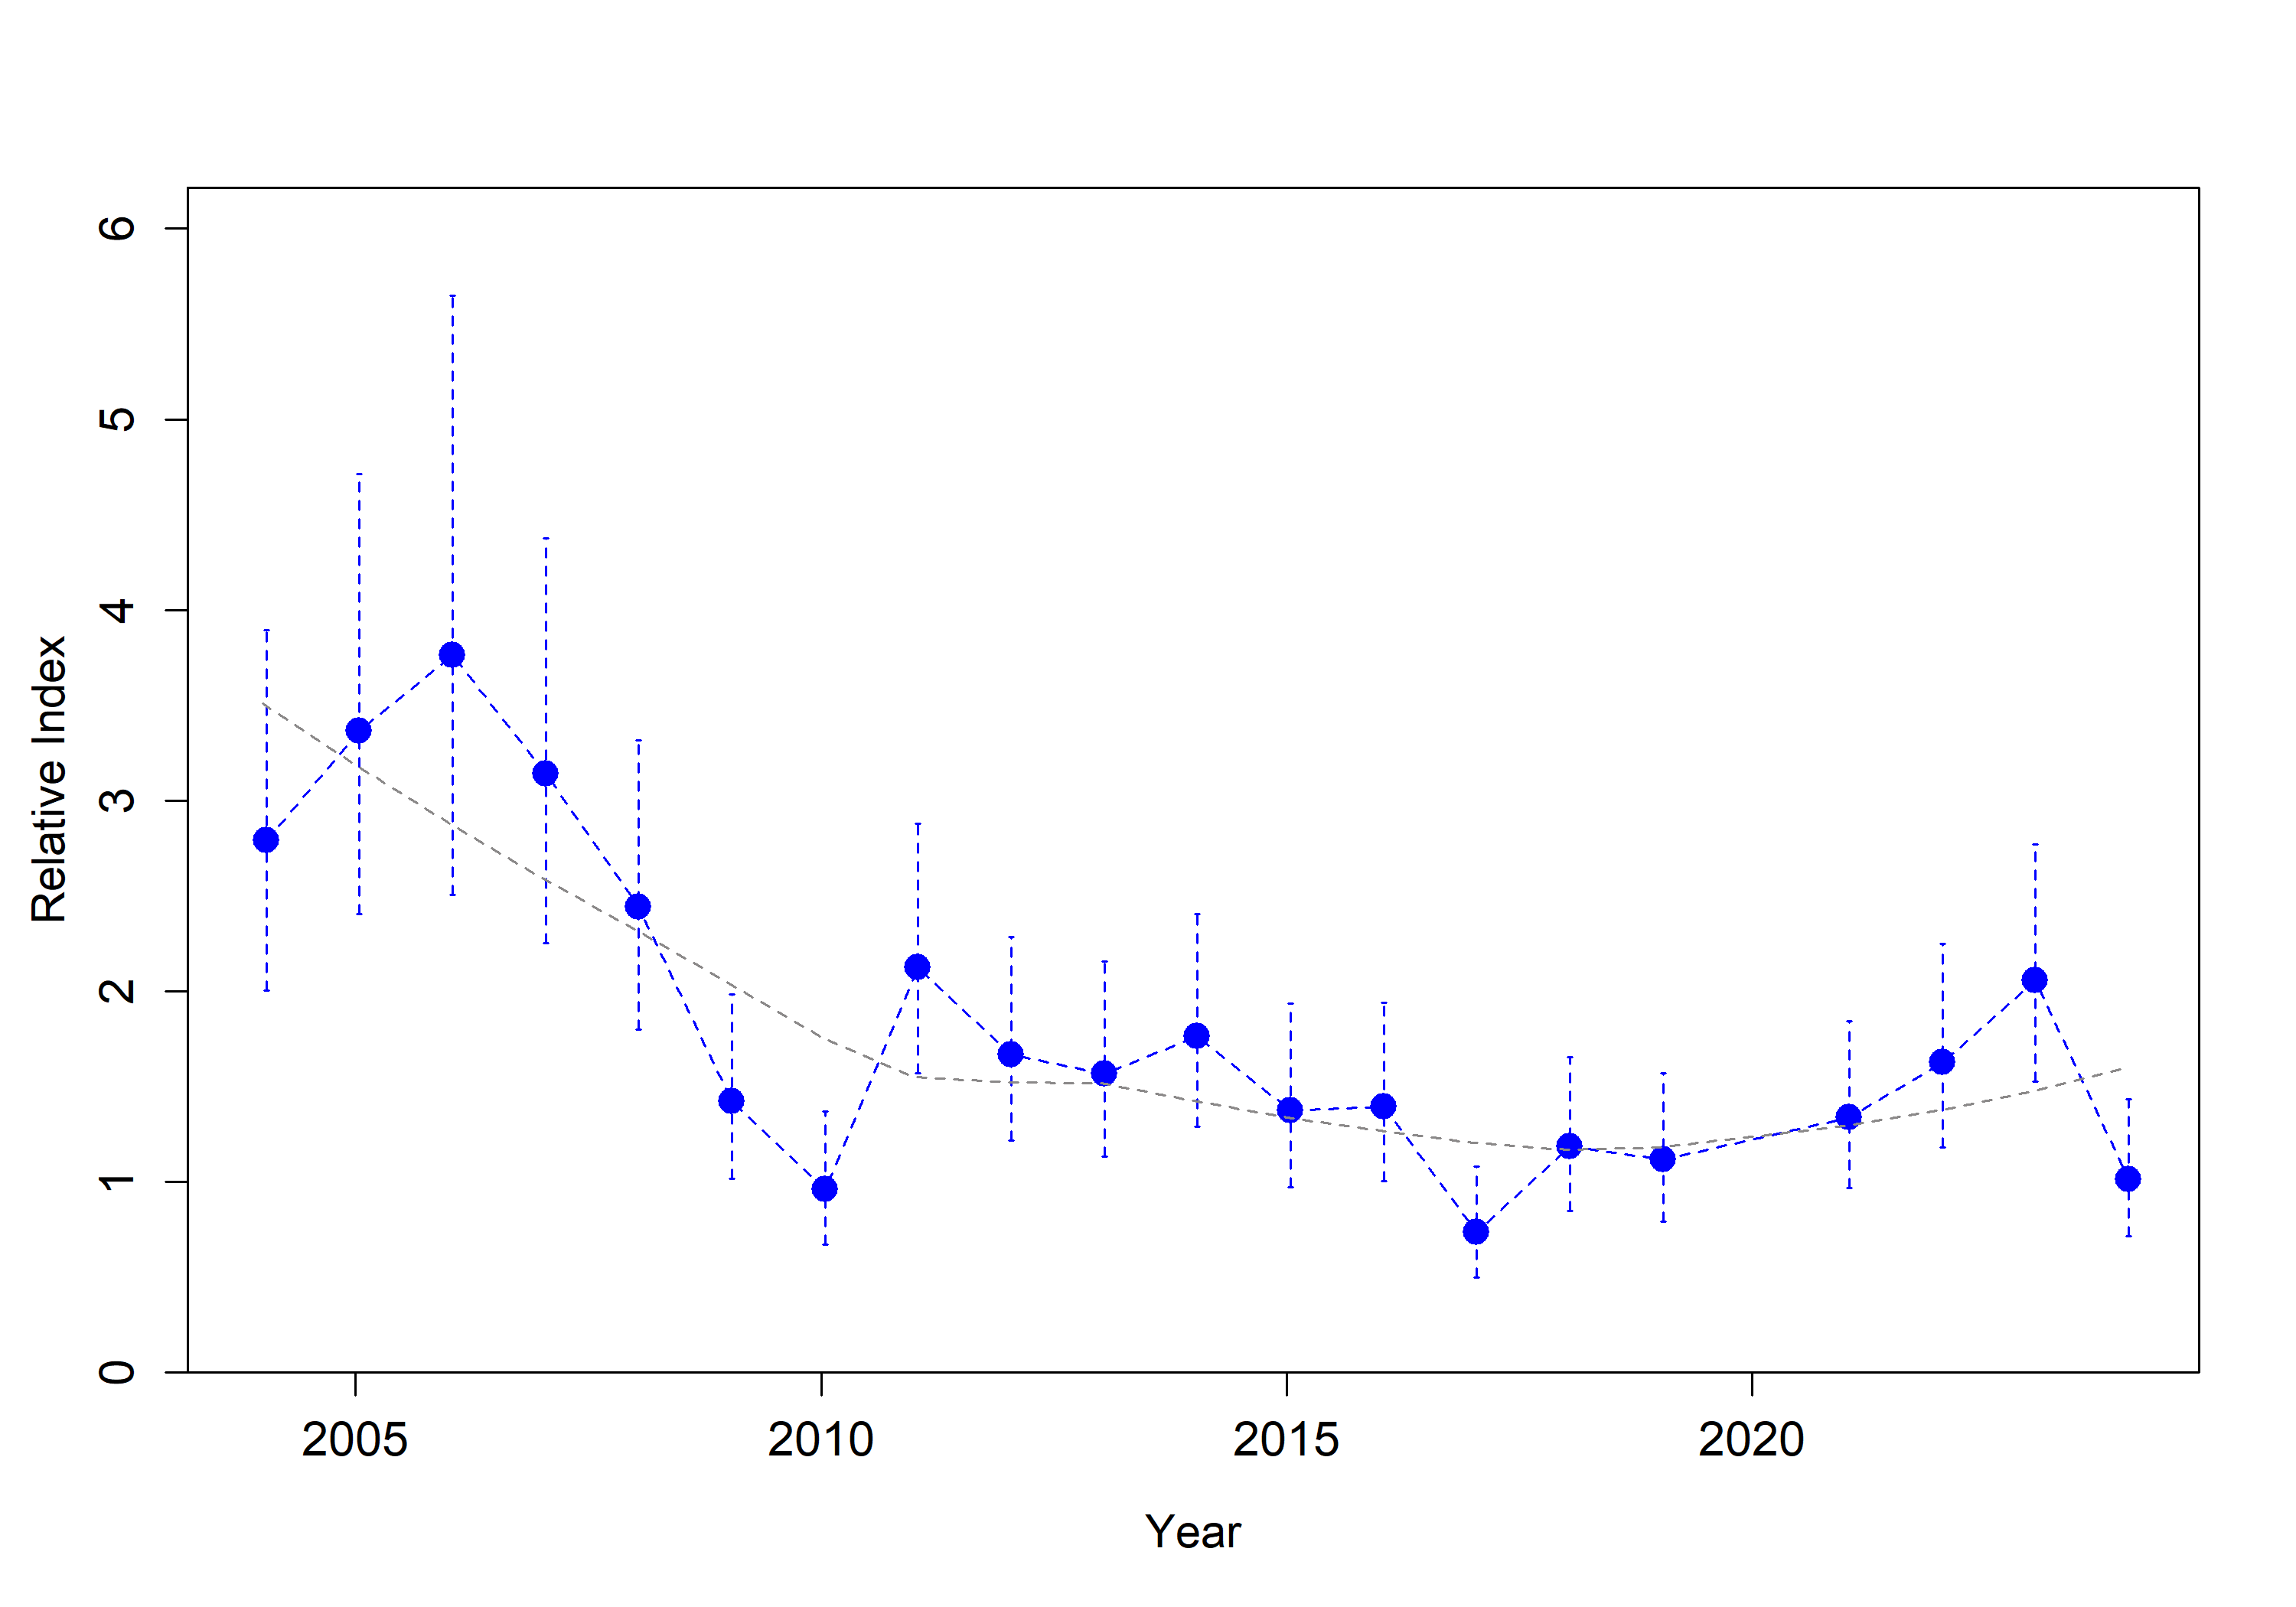
\includegraphics[width=0.95\linewidth,height=\textheight,keepaspectratio]{../plots/hkl_indices/yellowtail rockfish south_negbinom index.png}

}

\caption{Estimated relative index of abundance for yellowtail rockfish
south from the NWFSC HKLS.}

\end{figure}%

\begin{figure}[H]

{\centering 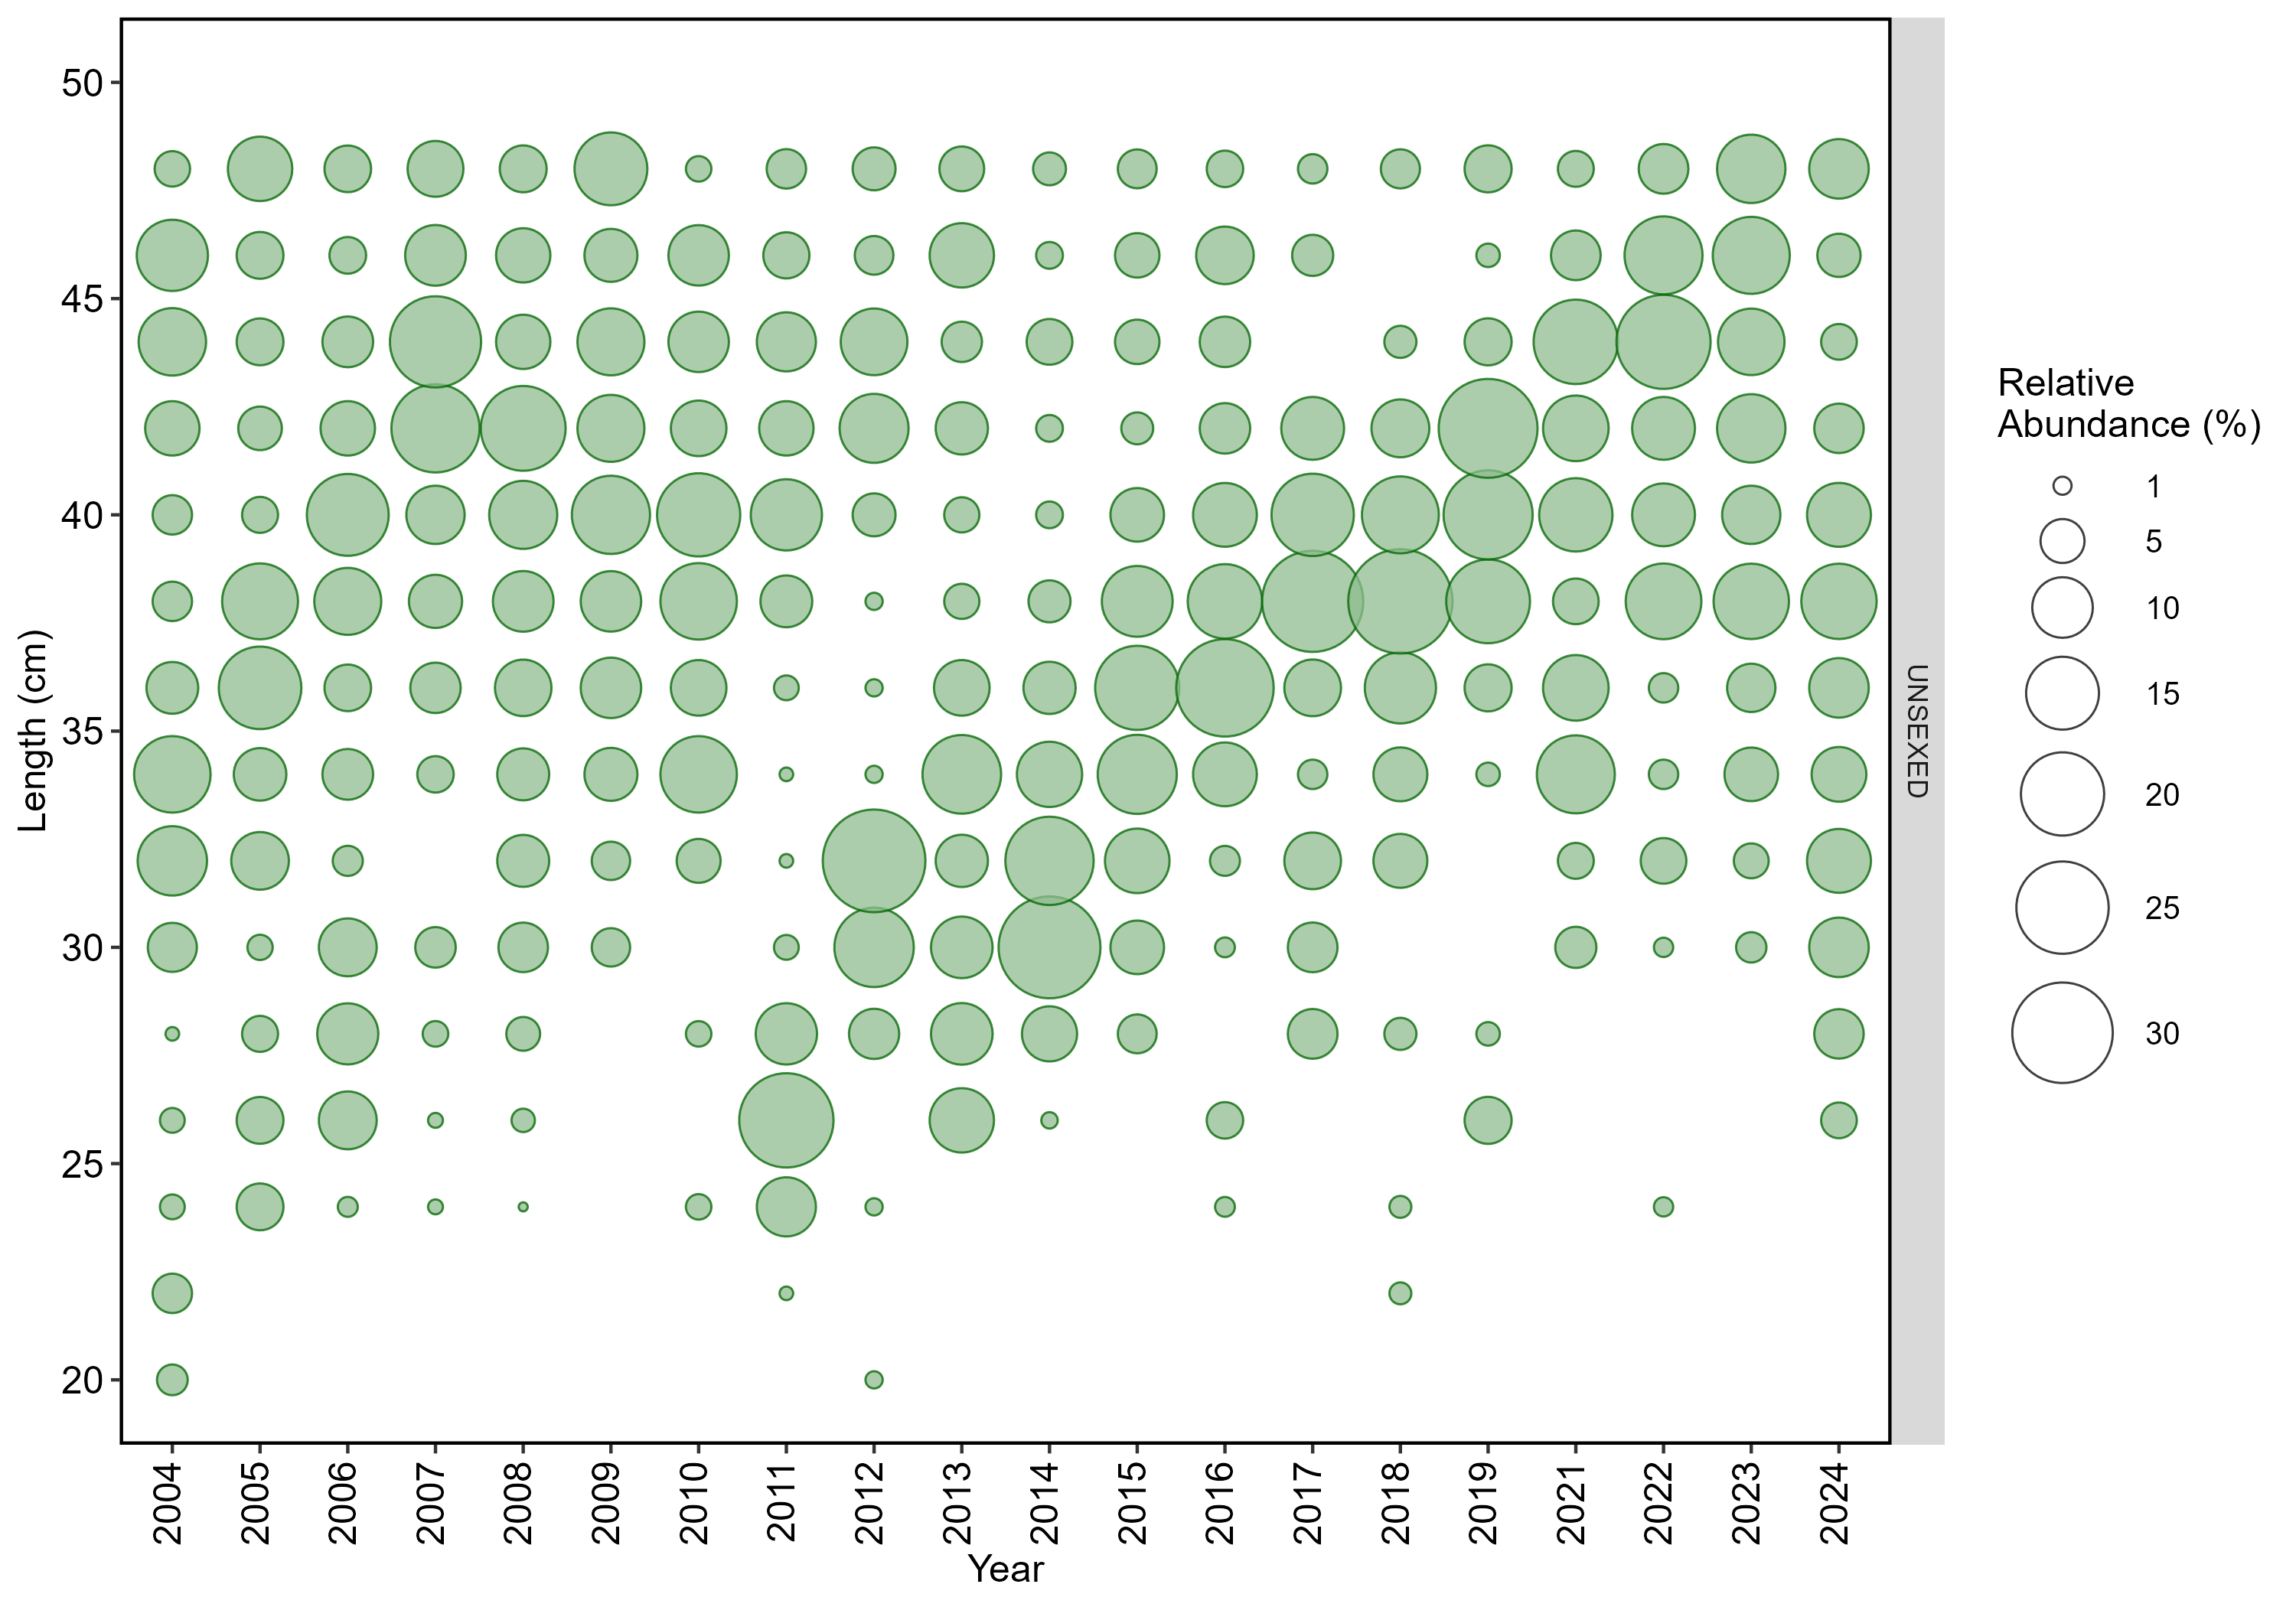
\includegraphics[width=0.95\linewidth,height=\textheight,keepaspectratio]{../plots/hkl_comps/plots/yellowtail rockfish south_nwfsc_hkl_length_frequency_sex_0.png}

}

\caption{Length (cm) compostion data from the NWFSC HKLS for yellowtail
rockfish south. Size of the circles within a year indicate higher
(larger circles) and lower (smaller circles) proportion observed by
length bin.}

\end{figure}%

\newpage{}

\section{Index Estimation for the NWFSC WCGBT
Survey}\label{wcgbt-index-settings}

\begingroup\fontsize{7}{9}\selectfont

\begin{landscape}\begingroup\fontsize{7}{9}\selectfont

\begin{longtable}[t]{>{\raggedright\arraybackslash}p{3 cm}>{\raggedright\arraybackslash}p{2 cm}>{\raggedright\arraybackslash}p{4 cm}>{\raggedright\arraybackslash}p{2 cm}>{\raggedright\arraybackslash}p{2 cm}>{\raggedright\arraybackslash}p{2 cm}>{\raggedright\arraybackslash}p{2 cm}>{\raggedright\arraybackslash}p{3 cm}>{\raggedright\arraybackslash}p{2 cm}>{\raggedright\arraybackslash}p{4 cm}>{\raggedright\arraybackslash}p{2 cm}>{\raggedright\arraybackslash}p{2 cm}>{\raggedright\arraybackslash}p{2 cm}>{\raggedright\arraybackslash}p{2 cm}>{\raggedright\arraybackslash}p{3 cm}>{\raggedright\arraybackslash}p{2 cm}>{\raggedright\arraybackslash}p{4 cm}}
\caption{\label{tab:survey-settings}Setting used for estimating indices of abundance for the NWFSC WCGBTS by species.}\\
\toprule
species & family & formula & min latitude & max latitude & spatiotemporal1 & spatiotemporal2\\
\midrule
\endfirsthead
\caption[]{Setting used for estimating indices of abundance for the NWFSC WCGBTS by species. (\textit{continued)}}\\
\toprule
species & family & formula & min latitude & max latitude & spatiotemporal1 & spatiotemporal2\\
\midrule
\endhead

\endfoot
\bottomrule
\endlastfoot
arrowtooth flounder & delta\_gamma() & catch\_weight \textasciitilde{} 0 + fyear + pass\_scaled & 34.0 & 49.0 & iid & iid\\
aurora rockfish & delta\_gamma() & catch\_weight \textasciitilde{} 0 + fyear + pass\_scaled & 31.9 & 49.0 & off & iid\\
big skate & delta\_gamma() & catch\_weight \textasciitilde{} 0 + fyear + pass\_scaled & 31.9 & 49.0 & iid & iid\\
blackgill rockfish & delta\_gamma() & catch\_weight \textasciitilde{} 0 + fyear & 35.0 & 49.0 & off & off\\
bocaccio & delta\_gamma() & catch\_weight \textasciitilde{} 0 + fyear + pass\_scaled & 31.9 & 49.0 & iid & iid\\
canary rockfish & delta\_lognormal() & catch\_weight \textasciitilde{} 0 + fyear + pass\_scaled & 31.9 & 49.0 & iid & off\\
chilipepper & delta\_lognormal() & catch\_weight \textasciitilde{} 0 + fyear + pass\_scaled + depth\_scaled + depth\_scaled\_squared & 31.9 & 46.2 & iid & off\\
curlfin sole & tweedie() & catch\_weight \textasciitilde{} 0 + fyear + pass\_scaled & 31.9 & 49.0 & iid & iid\\
darkblotched rockfish & delta\_lognormal() & catch\_weight \textasciitilde{} 0 + fyear + pass\_scaled & 33.5 & 49.0 & off & iid\\
Dover sole & delta\_gamma() & catch\_weight \textasciitilde{} 0 + fyear + pass\_scaled & 31.9 & 49.0 & iid & iid\\
English sole & delta\_gamma() & catch\_weight \textasciitilde{} 0 + fyear + pass\_scaled & 31.9 & 49.0 & iid & iid\\
flathead sole & delta\_gamma() & catch\_weight \textasciitilde{} 0 + fyear + pass\_scaled & 41.0 & 49.0 & iid & iid\\
greenspotted rockfish & delta\_lognormal() & catch\_weight \textasciitilde{} 0 + fyear & 31.9 & 49.0 & iid & iid\\
greenstriped rockfish & delta\_gamma() & catch\_weight \textasciitilde{} 0 + fyear & 31.9 & 49.0 & iid & iid\\
lingcod north & delta\_gamma() & catch\_weight \textasciitilde{} 0 + fyear + pass\_scaled & 40.2 & 49.0 & iid & iid\\
lingcod south & delta\_gamma() & catch\_weight \textasciitilde{} 0 + fyear + pass\_scaled & 31.9 & 40.2 & iid & iid\\
longnose skate & delta\_gamma() & catch\_weight \textasciitilde{} 0 + fyear + pass\_scaled & 31.9 & 49.0 & iid & iid\\
longspine thornyhead & delta\_lognormal() & catch\_weight \textasciitilde{} 0 + fyear + pass\_scaled + depth\_scaled + depth\_scaled\_squared & 31.9 & 49.0 & off & off\\
Pacific cod & delta\_gamma() & catch\_weight \textasciitilde{} 0 + fyear + pass\_scaled & 39.0 & 49.0 & iid & iid\\
Pacific ocean perch & delta\_gamma() & catch\_weight \textasciitilde{} 0 + fyear + pass\_scaled & 35.0 & 49.0 & iid & iid\\
Pacific sanddab & delta\_gamma() & catch\_weight \textasciitilde{} 0 + fyear + pass\_scaled & 31.9 & 49.0 & iid & iid\\
Pacific spiny dogfish & delta\_lognormal() & catch\_weight \textasciitilde{} 0 + fyear + pass\_scaled & 31.9 & 49.0 & iid & iid\\
petrale sole & delta\_lognormal() & catch\_weight \textasciitilde{} 0 + fyear + pass\_scaled & 31.9 & 49.0 & iid & iid\\
redbanded rockfish & delta\_gamma() & catch\_weight \textasciitilde{} 0 + fyear & 33.5 & 49.0 & off & iid\\
rex sole & delta\_gamma() & catch\_weight \textasciitilde{} 0 + fyear + pass\_scaled & 31.9 & 49.0 & iid & iid\\
rosethorn rockfish & delta\_gamma() & catch\_weight \textasciitilde{} 0 + fyear + pass\_scaled & 31.9 & 49.0 & off & off\\
rougheye and blackspotted rockfish & delta\_lognormal() & catch\_weight \textasciitilde{} 0 + fyear + pass\_scaled & 42.0 & 49.0 & off & off\\
sablefish & delta\_gamma() & catch\_weight \textasciitilde{} 0 + fyear + pass\_scaled & 31.9 & 49.0 & iid & iid\\
sharpchin rockfish & delta\_lognormal() & catch\_weight \textasciitilde{} 0 + fyear + pass\_scaled & 33.0 & 49.0 & iid & off\\
shortspine thornyhead & delta\_lognormal() & catch\_weight \textasciitilde{} 0 + fyear + pass\_scaled + depth\_scaled + depth\_scaled\_squared & 31.9 & 49.0 & iid & iid\\
splitnose rockfish & delta\_lognormal() & catch\_weight \textasciitilde{} 0 + fyear + pass\_scaled & 31.9 & 49.0 & iid & iid\\
stripetail rockfish & delta\_gamma() & catch\_weight \textasciitilde{} 0 + fyear & 31.9 & 49.0 & off & iid\\
widow rockfish & delta\_lognormal() & catch\_weight \textasciitilde{} 0 + fyear + pass\_scaled & 33.5 & 49.0 & iid & off\\
yelloweye rockfish & delta\_lognormal() & catch\_weight \textasciitilde{} 0 + fyear + pass\_scaled & 42.0 & 49.0 & off & off\\
yellowtail rockfish north & delta\_lognormal() & catch\_weight \textasciitilde{} 0 + fyear*split\_mendocino + pass\_scaled & 33.5 & 49.0 & iid & off\\*
\end{longtable}
\endgroup{}
\end{landscape}
\endgroup{}

\section{Index Estimation for the NWFSC Hook and Line
Survey}\label{hkl-index-settings}

Relative indices of abundance by species were estimated using
\texttt{sdmTMB} with a negative-binomial error structure and no spatial
or spatiotemporal effects. The included covariates accounted for year,
site, and drop
(\texttt{n\ \textasciitilde{}\ 0\ +\ year\ +\ site\_number\ +\ drop}).
Effort was defined as the product of the number of lines in the water
(e.g., fishing off the bow, stern, or mid-ship) and the number of hooks
by year, site, and drop number.

\newpage

\section{Acknowledgements}\label{acknowledgements}

We would like to thank the NWFSC Fisheries Resource Analysis and
Monitoring WCGBTS and HKLS teams, including volunteer biologists and
vessel captains and crew, and acknowledge their dedication to collecting
high quality data that are essential to the assessment of West Coast
groundfish stocks. Thank you to Eric Ward who was instrumental in
estimating indices for the large number of species in this report and
his dedication for improving workflows and automation.




\end{document}
